\documentclass[leqno,b5paper]{book}
%\usepackage{fancyhdr}   %put fancyhdr on jan-01-2015 and it worked
%\pagestyle{fancy}
%\usepackage[hidelinks]{hyperref}   %messes with equation numbers and their reference calls (RTL issues)
\usepackage{./tex/khalidUrduBooksMachines}                     %my sty file
\usepackage{pgfplots}

%============================
%\usepackage{newfile}                                                                  %collecting techniacalterms
%\newwrite\tempfileTerms
%\immediate\openout\tempfileTerms=technicalTerms.tex
%\newcommand*\wf[1]{\immediate\write\tempfileTerms{#1}}
%			%%collecting techinal terms
%\newcommand*{\اصطلاح}[1]{\wf{\unexpanded{ur, #1 ,}}}
%\newcommand*{\حاشیہب}[1]{ \wf{\unexpanded{en, #1,}}}
%================================
%=================================

%this file describes urdu commands for the commonly used english latex commands

%chapter, section etc
\newcommand*{\باب}[1]{\chapter{#1}}                                      %defining commonly used commands
\newcommand*{\حصہ}[1]{\section{#1}}
\newcommand*{\جزوحصہ}[1]{\subsection{#1}}
\newcommand*{\جزوجزوحصہ}[1]{\subsubsection{#1}}

\newcommand*{\بابء}[1]{\chapter*{#1}}                                      %defining commonly used commands
\newcommand*{\حصہء}[1]{\section*{#1}}
\newcommand*{\جزوحصہء}[1]{\subsection*{#1}}
\newcommand*{\جزوجزوحصہء}[1]{\subsubsection*{#1}}


%english text in urdu mode
\newcommand*{\تحریر}[1]{\textenglish{#1}}	% english text in urduMode
\newcommand*{\موٹا}[1]{\textbf{#1}}
\newcommand*{\ترچہ}[1]{{\textit{#1}}}
%%\newcommand*{\اصطلاح}[1]{{\textbf{#1}}}
\newcommand*{\اصطلاح}[1]{{\urduTechTermsfont{#1}}}

%end commands cannot be redefined and as such these two are not usable
\providecommand*{\ابتدا}[1]{\begin{#1}}
\providecommand*{\انتہا}[1]{\end{#1}}

%include and input directives for adding external files into the main document 
\newcommand*{\بشمول}[1]{\includeonly{#1}}
\newcommand*{\شامل}[1]{\include{#1}}
\newcommand*{\داخل}[1]{\input{#1}}

%to use extra latex packages
\newcommand*{\استعمال}[1]{\usepackage{#1}}

%footnotes and indexes
\newcommand*{\حاشیہب}[1]{{\raggedright{\footnote{\textenglish{#1}}}} }               %footnote to the left hand side
\newcommand*{\حاشیہد}[1]{{\raggedleft{\footnote{#1}}}}
\newcommand*{\حاشیہط}[1]{\marginpar{#1}}

\newcommand*{\فرہنگ}[1]{\index{#1}}

%references and labels
\newcommand*{\شناخت}[1]{\label{#1}}
\newcommand*{\حوالہ}[1]{\textenglish{\ref{#1}}}
\newcommand*{\حوالہصفحہ}[1]{\pageref{#1}}

%counters
\newcommand*{\فاصلہ}{\vspace*{10mm}}

%itemize, bullets and numbered items   
\newcommand*{\اشیاء}{itemize}                               %used in   \begin{itemize}
\newcommand*{\شے}[1]{\item {#1}}			%used in    \item

%maths commands
%\newcommand*{\عددی}[1]{\: \ensuremath{#1} \:} % in-line math & inside math mode
%\newcommand*{\عددیء}[1]{\ensuremath{#1}}
\newcommand*{\عددی}[1]{\: \(#1\) \:} % in-line math & inside math mode
\newcommand*{\عددیء}[1]{\(#1\)}
%\newcommand*{\سمتیہ}[1]{\ensuremath{\bf{#1}}}
\newcommand*{\سمتیہ}[1]{{\ensuremath{{\boldsymbol{#1}}}}}
\newcommand*{\سمتیہز}[2]{{\ensuremath{{\boldsymbol{#1}_{#2}}}}}     %with non-vector subscript
\newcommand*{\ضرب}{\time}					%multiplication symbol
\newcommand*{\نکطہد}{\cdot}
\newcommand*{\نقطے}{\ensuremath{\cdots}}

\newcommand*{\زیرنوشت}[3]{\: \ensuremath{{#1_{#2 \textrm {#3}}}} \:}   %english+urdu subscript \زیرنوشت{V}{CE}{غیرافزائندہ}
\newcommand*{\سیدھازیرنوشت}[2]{\: \ensuremath{{#1_{\textup{#2}}}} \:} %RC

\newcommand*{\قریب}[1]{\mbox{#1}}
\newcommand{\سن}[1]{؁\,\ensuremath{#1}}

\newcommand{\kQuote}[1]{“#1”}
\newcommand{\kquote}[1]{‘#1’}
\newcommand{\قولء}[1]{’#1‘}
\newcommand{\قول}[1]{”#1“}

\renewcommand{\indexname}{فرہنگ}        %apparently did nothing


%%numbering scheme
%\renewcommand*{\thefigure}{\thechapter.\arabic{figure}}
%\renewcommand*{\thetable}{\thechapter.\arabic{table}}
%\renewcommand*{\theequation}{\thechapter.\arabic{equation}}
%\renewcommand*{\thesection}{\thechapter.\arabic{section}}
%\renewcommand*{\thesubsection}{\thechapter.\arabic{section}.\arabic{subsection}}
%\renewcommand*{\thesubsubsection}{\thechapter.\arabic{section}.\arabic{subsection}.\arabic{subsubsection}}

%================
%my environments
%================

%environment for examples مثال
%\newcounter{examplecounter}[section]
%\renewcommand{\theexamplecounter}{\arabic{examplecounter}}
\newcounter{examplecounter}[chapter]
\renewcommand{\theexamplecounter}{\thechapter.\arabic{examplecounter}}

\newenvironment*{مثال}
{\par\noindent\ignorespaces    مثال \refstepcounter{examplecounter} \theexamplecounter :\quad}%
{\hfill\qedsymbol  \vspace{\baselineskip}\par}
%{\noindent\ignorespaces \vspace{\baselineskip} \hrule \vspace{\baselineskip}  مثال \refstepcounter{examplecounter} \theexamplecounter :}%
%{\par\noindent \hrule  \vspace{\baselineskip}}

%------
%practice problems environment مشق

%\newcounter{practicecounter}[section]                              %practice here means مشق
%\renewcommand{\thepracticecounter}{\arabic{practicecounter}}
\newcounter{practicecounter}[chapter]                              %practice here means مشق
\renewcommand{\thepracticecounter}{\thechapter.\arabic{practicecounter}}

\newenvironment*{مشق}
{\par\noindent\ignorespaces \vspace{\baselineskip} \hrule \vspace{\baselineskip} مشق \refstepcounter{practicecounter} \thepracticecounter :\quad}%
{\par\noindent \hrule  \vspace{\baselineskip}}
%---------

%end of chapter questions environment سوال

\newcounter{questioncounter}[section]                                           %for reseting at every section. to be used only during writing stage
\renewcommand{\thequestioncounter}{\arabic{questioncounter}}
%\newcounter{questioncounter}[chapter]						%when book is finished, use this instead of the above
%\renewcommand{\thequestioncounter}{\thechapter.\arabic{questioncounter}}

\newenvironment*{سوال}				
{\noindent\ignorespaces  سوال \refstepcounter{questioncounter} \thequestioncounter :\quad}%
{\par\noindent\ignorespaces }
%--------------------

%defining a LAW   قانون

%\newcounter{lawcounter}[section]
%\renewcommand{\thelawcounter}{\arabic{lawcounter}}
\newcounter{lawcounter}[chapter]
\renewcommand{\thelawcounter}{\thechapter.\arabic{lawcounter}}

\newenvironment*{قانون}				
{\par\medskip \refstepcounter{lawcounter} \quad\nopagebreak}%
{\par\hfill\qedsymbol  \vspace{\baselineskip}\par }
%{\par\medskip }
%--------------------
%--------------------

%defining a THEOREM   مسئلہ

%\newcounter{kthcounter}[section]
%\renewcommand{\thekthcounter}{\arabic{kthcounter}}
\newcounter{kthcounter}[chapter]
\renewcommand{\thekthcounter}{\thechapter.\arabic{kthcounter}}

\newenvironment*{مسئلہ}				
{\par\noindent\ignorespaces  مسئلہ \refstepcounter{kthcounter} \thekthcounter :\quad}%
{\par\noindent }
%--------------------
%--------------------

%defining a Proof   ثبوت

%\newcounter{kprcounter}[chapter]
%\renewcommand{\thekprcounter}{\thechapter.\arabic{kprcounter}}

\newenvironment*{ثبوت}				
{\noindent\ignorespaces  ثبوت :\quad}%
{\par\hfill\qedsymbol  \vspace{\baselineskip}\par }
%{\par\noindent\qedsymbol  \vspace{\baselineskip} }
%--------------------
%--------------------
%++++++++++++++++++++++++++++++

%--------------------

%defining a COROLLARY   ضمنی نتیجہ


\newcounter{kcocounter}[chapter]
\renewcommand{\thekcocounter}{\thechapter.\arabic{kcocounter}}

\newenvironment*{ضمنی نتیجہ}				
{\par\noindent\ignorespaces  ضمنی نتیجہ \refstepcounter{kcocounter} \thekcocounter :\quad}%
{\par\noindent }
%--------------------
%--------------------

%defining a Proof   ثبوت ضمنی نتیجہ

%\newcounter{kprcocounter}[chapter]
%\renewcommand{\thekprcocounter}{\thechapter.\arabic{kprcocounter}}

\newenvironment*{ثبوت ضمنی نتیجہ}				
{\noindent\ignorespaces  ثبوت ضمنی نتیجہ :\quad}%
{\par\hfill\qedsymbol  \vspace{\baselineskip}\par }
%{\par\noindent\qedsymbol  \vspace{\baselineskip} }
%--------------------
%--------------------
%++++++++++++++++++++++++++++++++++++++++++++

%defining a Definition تعریف

%\newcounter{kdfcounter}[chapter]
%\renewcommand{\thedfrcounter}{\thechapter.\arabic{kdfcounter}}

\newenvironment*{تعریف}				
{\par\noindent\ignorespaces  تعریف :\quad}%
{\par\hfill\qedsymbol  \vspace{\baselineskip}\par }
%{\par\noindent }
%--------------------
%----------------------------
%defining a Definition تعریفات

%\newcounter{kdfcounter}[chapter]
%\renewcommand{\thedfrcounter}{\thechapter.\arabic{kdfcounter}}

\newenvironment*{تعریفات}				
{\par\noindent\ignorespaces  تعریفات :\quad}%
{\par\hfill\qedsymbol  \vspace{\baselineskip}\par }
%{\par\noindent }
%--------------------
%--------------------

%defining a Definition مفروضہ

%\newcounter{kAscounter}[chapter]
%\renewcommand{\theAsrcounter}{\thechapter.\arabic{kAscounter}}

\newenvironment*{مفروضہ}				
{\par\noindent\ignorespaces  مفروضہ \quad}%
{\par\hfill\qedsymbol  \vspace{\baselineskip}\par }
%{\par\noindent }
%--------------------
%--------------------

%defining a RULE   قاعدہ

%\newcounter{krucounter}[section]
%\renewcommand{\thekrucounter}{\arabic{krucounter}}
\newcounter{krucounter}[chapter]
\renewcommand{\thekrucounter}{\thechapter.\arabic{krucounter}}

\newenvironment*{قاعدہ}				
{\par\noindent\ignorespaces  قاعدہ \refstepcounter{krucounter} \thekrucounter :\quad}%
{\par\noindent }
%--------------------
%--------------------

%defining a Proof   ثبوت قاعدہ

%\newcounter{kprRcounter}[chapter]
%\renewcommand{\thekprRcounter}{\thechapter.\arabic{kprRcounter}}

\newenvironment*{ثبوت قاعدہ}				
{\noindent\ignorespaces  ثبوت قاعدہ :\quad}%
{\par\hfill\qedsymbol  \vspace{\baselineskip}\par }
%{\par\noindent\qedsymbol  \vspace{\baselineskip} }
%--------------------
%--------------------

%defining a TEST   پرکھ

%\newcounter{kttcounter}[section]
%\renewcommand{\thekttcounter}{\arabic{kttcounter}}
\newcounter{kttcounter}[chapter]
\renewcommand{\thekttcounter}{\thechapter.\arabic{kttcounter}}

\newenvironment*{پرکھ}				
{\par\noindent\ignorespaces  \refstepcounter{kttcounter} \quad \nopagebreak}%
{\par\hfill\qedsymbol  \vspace{\baselineskip}\par }
%--------------------

\newenvironment*{ثبوت پرکھ}				
{\noindent\ignorespaces  ثبوت پرکھ :\quad}%
{\par\hfill\qedsymbol  \vspace{\baselineskip}\par }
%{\par\noindent\qedsymbol  \vspace{\baselineskip} }

%---------

%questions environment جواب

%\newcounter{answercounter}[section]                                           %for reseting at every section. NOT NEEDED
%\renewcommand{\theanswercounter}{\arabic{answercounter}}
%\newcounter{answercounter}[chapter]						%when book is finished, use this instead of the above
%\renewcommand{\theanswercounter}{\thechapter.\arabic{answercounter}}

%\newenvironment*{جواب}				
%{\noindent\ignorespaces\wf{\thequestioncounter)\noexpand\quad}}%
%{\par\noindent\ignorespacesafterend}
%==================

\newenvironment*{سوالات}				
{\noindent\ignorespaces\wf{
\موٹا{حصہ} 
\thesection
\quad
\موٹا{صفحہ}
\thepage}
\wf{\unexpanded{\begin{description}\setlength{\parskip}{0pt} \setlength{\itemsep}{0pt plus 1pt}}}
}%
{\wf{\unexpanded{\end{description}}}\par\noindent\ignorespacesafterend}
%==================
\newenvironment*{جواب}				
{\noindent\ignorespaces\wf{\unexpanded{\item[}}\wf{\thequestioncounter)}\wf{\unexpanded{]}}}%
{\noindent\ignorespacesafterend}
%==================
\newenvironment*{جوابء}				
{\noindent\ignorespaces\wf{\unexpanded{[}}\wf{\thequestioncounter)}\wf{\unexpanded{]}}}%
{\par\noindent\ignorespacesafterend}
%==================

                  %turning latex into urdu
%%this file describes urdu commands for the commonly used english latex commands

%chapter, section etc
%  \newcommand*{newcommand}[arguments]{actual command}
\newcommand*{\باب}[1]{\chapter{#1}}                                      %defining commonly used commands
\newcommand*{\حصہ}[1]{\section{#1}}
\newcommand*{\جزوحصہ}[1]{\subsection{#1}}
\newcommand*{\جزوجزوحصہ}[1]{\subsubsection{#1}}

\newcommand*{\بابء}[1]{\chapter*{#1}}                                      %defining commonly used commands
\newcommand*{\حصہء}[1]{\section*{#1}}
\newcommand*{\جزوحصہء}[1]{\subsection*{#1}}
\newcommand*{\جزوجزوحصہء}[1]{\subsubsection*{#1}}


%english text in urdu mode
\newcommand*{\تحریر}[1]{\textenglish{#1}}	% english text in urduMode
%\newcommand*{\موٹا}[1]{\textbf{#1}}
%\newcommand*{\ترچھا}[1]{{\textit{#1}}}
\newcommand*{\موٹا}[1]{{\urduTechTermsfont{#1}}}
\newcommand*{\ترچھا}[1]{{\small{#1}}}

%%\newcommand*{\اصطلاح}[1]{{\color{red}{#1}}}   %colours spills to next word when there is index or footnote entry with the word
%%\newcommand{\اصطلاح}[1]{{\urdufontBig{#1}}}

\newcommand{\اصطلاح}[1]{{\urduTechTermsfont{#1}}}  %%%moved to main file
\newcommand{\اصطلاحء}[1]{{\small{#1}}} %highlighted where  chance of mixup with  regular urdu meaning


%end commands cannot be redefined and as such these two are not usable
\providecommand*{\ابتدا}[1]{\begin{#1}}
\providecommand*{\انتہا}[1]{\end{#1}}

%include and input directives for adding external files into the main document 
\newcommand*{\بشمول}[1]{\includeonly{#1}}
\newcommand*{\شامل}[1]{\include{#1}}
\newcommand*{\داخل}[1]{\input{#1}}

%to use extra latex packages
\newcommand*{\استعمال}[1]{\usepackage{#1}}

%footnotes and indexes
\newcommand*{\حاشیہب}[1]{{\raggedright{\footnote{\textenglish{#1}}}} }          %  moved to main file. footnote to the left hand side
\newcommand*{\حاشیہد}[1]{{\raggedleft{\footnote{#1}}}}
\newcommand*{\حاشیہط}[1]{\marginpar{#1}}

\newcommand*{\فرہنگ}[1]{\index{#1}}

%references and labels
\newcommand*{\شناخت}[1]{\label{#1}}
\newcommand*{\حوالہ}[1]{\ref{#1}}
\newcommand*{\حوالہء}[1]{#1}			%dummy to enter the figure number directly while the figure is not ready
\newcommand*{\حوالہصفحہ}[1]{\pageref{#1}}

%counters
\newcommand*{\فاصلہ}{\vspace*{10mm}}
\newcommand*{\فاصلہء}{\quad}

%itemize, bullets and numbered items   
\newcommand*{\اشیاء}{itemize}                               %used in   \begin{itemize}
\newcommand*{\شے}[1]{\item {#1}}			%used in    \item, \description
%description
\newcommand*{\جزو}[1]{\item[#1]}                      %used in \begin{description}
%maths commands
\newcommand*{\عددی}[1]{\: \ensuremath{#1} \:} % in-line math & inside math mode
\newcommand*{\عددیء}[1]{\ensuremath{#1}}
\newcommand*{\سمتیہ}[1]{\ensuremath{{\bf{#1}}}}
\newcommand*{\سمتیازیرنوشت}[2]{\ensuremath{{\boldsymbol{#1}}_{\textup{#2}}}}

\newcommand*{\ضرب}{\time}					%multiplication symbol
\newcommand*{\نکطہد}{\cdot}
\newcommand*{\نقطے}{\ensuremath{\cdots}}

\newcommand*{\زیرنوشت}[3]{\: \ensuremath{{#1_{#2 \textrm {#3}}}} \:}   %english+urdu subscript \زیرنوشت{V}{CE}{غیرافزائندہ}
\newcommand*{\سیدھازیرنوشت}[2]{\: \ensuremath{{#1_{\textup{#2}}}} \:} %RC

\newcommand*{\قریب}[1]{\mbox{#1}}  %dissallows splitting along two lines 
\newcommand{\سن}[1]{؁\,\ensuremath{#1}}
\newcommand{\زور}[1]{\aemph{#1}} %overline urdu text to emphasize


\renewcommand{\indexname}{فرہنگ}        %does nothing here. must be placed within begin{urdufont} environment to be the last to take effect 
%===============================


%=======================================


%================
%my environments
%================

%environment for examples مثال
%\newcounter{examplecounter}[section]
%\renewcommand{\theexamplecounter}{\arabic{examplecounter}}
\newcounter{examplecounter}[chapter]
\renewcommand{\theexamplecounter}{\thechapter.\arabic{examplecounter}}

\newenvironment*{مثال}
{\par\noindent\ignorespaces    مثال \refstepcounter{examplecounter} \theexamplecounter :\quad}%
{\hfill\qedsymbol  \vspace{\baselineskip}\par}
%{\noindent\ignorespaces \vspace{\baselineskip} \hrule \vspace{\baselineskip}  مثال \refstepcounter{examplecounter} \theexamplecounter :}%
%{\par\noindent \hrule  \vspace{\baselineskip}}

%------
%practice problems environment مشق

%\newcounter{practicecounter}[section]                              %practice here means مشق
%\renewcommand{\thepracticecounter}{\arabic{practicecounter}}
\newcounter{practicecounter}[chapter]                              %practice here means مشق
\renewcommand{\thepracticecounter}{\thechapter.\arabic{practicecounter}}

\newenvironment*{مشق}
{\par\noindent\ignorespaces \vspace{\baselineskip} \hrule \vspace{\baselineskip} مشق \refstepcounter{practicecounter} \thepracticecounter :\quad}%
{\par\noindent \hrule  \vspace{\baselineskip}}
%---------

%end of chapter questions environment سوال

\newcounter{questioncounter}[chapter]                           %for reseting at every section. to be used only during writing stage
%\renewcommand{\thequestioncounter}{\arabic{questioncounter}}
%\newcounter{questioncounter}[chapter]						%when book is finished, use this instead of the above
\renewcommand{\thequestioncounter}{\thechapter.\arabic{questioncounter}}

\newenvironment*{سوال}				
{\noindent\ignorespaces  سوال \refstepcounter{questioncounter} \thequestioncounter :\quad}%
{\par\noindent\ignorespaces }
%--------------------

%defining a LAW   قانون

%\newcounter{lawcounter}[section]
%\renewcommand{\thelawcounter}{\arabic{lawcounter}}
\newcounter{lawcounter}[chapter]
\renewcommand{\thelawcounter}{\thechapter.\arabic{lawcounter}}

\newenvironment*{قانون}				
{\par\medskip \refstepcounter{lawcounter} \quad\nopagebreak}%
{\par\hfill\qedsymbol  \vspace{\baselineskip}\par }
%{\par\medskip }
%--------------------
%--------------------

%defining a THEOREM   مسئلہ

%\newcounter{kthcounter}[section]
%\renewcommand{\thekthcounter}{\arabic{kthcounter}}
\newcounter{kthcounter}[chapter]
\renewcommand{\thekthcounter}{\thechapter.\arabic{kthcounter}}

\newenvironment*{مسئلہ}				
{\par\noindent\ignorespaces  مسئلہ \refstepcounter{kthcounter} \thekthcounter :\quad}%
{\par\noindent }
%--------------------
%--------------------

%defining a Proof   ثبوت

%\newcounter{kprcounter}[chapter]
%\renewcommand{\thekprcounter}{\thechapter.\arabic{kprcounter}}

\newenvironment*{ثبوت}				
{\noindent\ignorespaces  ثبوت :\quad}%
{\par\hfill\qedsymbol  \vspace{\baselineskip}\par }
%{\par\noindent\qedsymbol  \vspace{\baselineskip} }
%--------------------
%--------------------
%++++++++++++++++++++++++++++++

%--------------------

%defining a COROLLARY   ضمنی نتیجہ


\newcounter{kcocounter}[chapter]
\renewcommand{\thekcocounter}{\thechapter.\arabic{kcocounter}}

\newenvironment*{ضمنی نتیجہ}				
{\par\noindent\ignorespaces  ضمنی نتیجہ \refstepcounter{kcocounter} \thekcocounter :\quad}%
{\par\noindent }
%--------------------
%--------------------

%defining a Proof   ثبوت ضمنی نتیجہ

%\newcounter{kprcocounter}[chapter]
%\renewcommand{\thekprcocounter}{\thechapter.\arabic{kprcocounter}}

\newenvironment*{ثبوت ضمنی نتیجہ}				
{\noindent\ignorespaces  ثبوت ضمنی نتیجہ :\quad}%
{\par\hfill\qedsymbol  \vspace{\baselineskip}\par }
%{\par\noindent\qedsymbol  \vspace{\baselineskip} }
%--------------------
%--------------------
%++++++++++++++++++++++++++++++++++++++++++++

%defining a Definition تعریف

%\newcounter{kdfcounter}[chapter]
%\renewcommand{\thedfrcounter}{\thechapter.\arabic{kdfcounter}}

\newenvironment*{تعریف}				
{\par\noindent\ignorespaces  تعریف :\quad}%
{\par\hfill\qedsymbol  \vspace{\baselineskip}\par }
%{\par\noindent }
%--------------------
%----------------------------
%defining a Definition تعریفات

%\newcounter{kdfcounter}[chapter]
%\renewcommand{\thedfrcounter}{\thechapter.\arabic{kdfcounter}}

\newenvironment*{تعریفات}				
{\par\noindent\ignorespaces  تعریفات :\quad}%
{\par\hfill\qedsymbol  \vspace{\baselineskip}\par }
%{\par\noindent }
%--------------------
%--------------------

%defining a Definition مفروضہ

%\newcounter{kAscounter}[chapter]
%\renewcommand{\theAsrcounter}{\thechapter.\arabic{kAscounter}}

\newenvironment*{مفروضہ}				
{\par\noindent\ignorespaces  مفروضہ \quad}%
{\par\hfill\qedsymbol  \vspace{\baselineskip}\par }
%{\par\noindent }
%--------------------
%--------------------

%defining a RULE   قاعدہ

%\newcounter{krucounter}[section]
%\renewcommand{\thekrucounter}{\arabic{krucounter}}
\newcounter{krucounter}[chapter]
\renewcommand{\thekrucounter}{\thechapter.\arabic{krucounter}}

\newenvironment*{قاعدہ}				
{\par\noindent\ignorespaces  قاعدہ \refstepcounter{krucounter} \thekrucounter :\quad}%
{\par\noindent }
%--------------------
%--------------------

%defining a Proof   ثبوت قاعدہ

%\newcounter{kprRcounter}[chapter]
%\renewcommand{\thekprRcounter}{\thechapter.\arabic{kprRcounter}}

\newenvironment*{ثبوت قاعدہ}				
{\noindent\ignorespaces  ثبوت قاعدہ :\quad}%
{\par\hfill\qedsymbol  \vspace{\baselineskip}\par }
%{\par\noindent\qedsymbol  \vspace{\baselineskip} }
%--------------------
%--------------------

%defining a TEST   پرکھ

%\newcounter{kttcounter}[section]
%\renewcommand{\thekttcounter}{\arabic{kttcounter}}
\newcounter{kttcounter}[chapter]
\renewcommand{\thekttcounter}{\thechapter.\arabic{kttcounter}}

\newenvironment*{پرکھ}				
{\par\noindent\ignorespaces  \refstepcounter{kttcounter} \quad \nopagebreak}%
{\par\hfill\qedsymbol  \vspace{\baselineskip}\par }
%--------------------

\newenvironment*{ثبوت پرکھ}				
{\noindent\ignorespaces  ثبوت پرکھ :\quad}%
{\par\hfill\qedsymbol  \vspace{\baselineskip}\par }
%{\par\noindent\qedsymbol  \vspace{\baselineskip} }

%---------

%questions environment جواب

%\newcounter{answercounter}[section]                                           %for reseting at every section. NOT NEEDED
%\renewcommand{\theanswercounter}{\arabic{answercounter}}
%\newcounter{answercounter}[chapter]						%when book is finished, use this instead of the above
%\renewcommand{\theanswercounter}{\thechapter.\arabic{answercounter}}

%\newenvironment*{جواب}				
%{\noindent\ignorespaces\wf{\thequestioncounter)\noexpand\quad}}%
%{\par\noindent\ignorespacesafterend}
%==================

\newenvironment*{سوالات}				
{\noindent\ignorespaces\wf{
\موٹا{حصہ} 
\thesection
\quad
\موٹا{صفحہ}
\thepage}
\wf{\unexpanded{\begin{description}\setlength{\parskip}{0pt} \setlength{\itemsep}{0pt plus 1pt}}}
}%
{\wf{\unexpanded{\end{description}}}\par\noindent\ignorespacesafterend}
%==================
\newenvironment*{جواب}  %the next is a better environment. it take less input		
{\noindent\ignorespaces\wf{\unexpanded{\item[}}\wf{\thequestioncounter)}\wf{\unexpanded{]}}}%
{\noindent\ignorespacesafterend}
%%==================
%%==================
%%this takes one input hence there is no need to write \wf{\unexpanded{...}} in every answer
%\newenvironment*{جواب}[1]			%put actual answer in {} examples {\(\sqrt{2}\)} 	
%{\noindent\ignorespaces\wf{\unexpanded{\item[}}\wf{\thequestioncounter)}\wf{\unexpanded{]}}\wf{\unexpanded{#1}}}%
%{\noindent\ignorespacesafterend}
%==================
%\newenvironment*{جوابء}				%i think is wrong and not used	
%{\noindent\ignorespaces\wf{\unexpanded{[}}\wf{\thequestioncounter)}\wf{\unexpanded{]}}}%
%{\par\noindent\ignorespacesafterend}
%==================

                  %turning latex into urdu
% Greek Letters for Urdu Latex usage

\newcommand*{\ایلفا}{\alpha}
\newcommand*{\بیٹا}{\beta}
\newcommand*{\گیما}{\gamma}
\newcommand*{\ڈیلٹا}{\delta}
\newcommand*{\ایپسلان}{\epsilon}
\newcommand*{\متغیرایپسلان}{\varepsilon}
\newcommand*{\زیٹا}{\zeta}
\newcommand*{\ایٹا}{\eta}
\newcommand*{\تھیٹا}{\theta}
\newcommand*{\متغیرتھیٹا}{\vartheta}
\newcommand*{\ایوٹا}{\iota}
\newcommand*{\کاپا}{\kappa}
\newcommand*{\لیمڈا}{\lambda}
\newcommand*{\میو}{\mu}
\newcommand*{\نیو}{\nu}
\newcommand*{\ژاے}{\xi}
\newcommand*{\پاے}{\pi}
\newcommand*{\متغیرپاے}{\varpi}
\newcommand*{\رھو}{\rho}
\newcommand*{\متغیررھو}{\varrho}
\newcommand*{\سگما}{\sigma}
\newcommand*{\متغیرسگما}{\varsigma}
\newcommand*{\ٹو}{\tau}
\newcommand*{\اپسیلان}{\upsilon}
\newcommand*{\فاے}{\phi}
\newcommand*{\متغیفاے}{\varphi}
\newcommand*{\چاے}{\chi}
\newcommand*{\ساے}{\psi}
\newcommand*{\اومیگا}{\omega}

\newcommand*{\بڑاگیما}{\Gamma}
\newcommand*{\بڑاڈیلٹا}{\Delta}
\newcommand*{\بڑاتھیٹا}{\Theta}
\newcommand*{\بڑالیمڈا}{\Lambda}
\newcommand*{\بڑاژاے}{\Xi}
\newcommand*{\بڑاپاے}{\Pi}
\newcommand*{\بڑاسگما}{\Sigma}
\newcommand*{\بڑاساے}{\Psi}
\newcommand*{\بڑااومیگا}{\Omega}



\newcommand*{\kvec}[1]{{\ensuremath{{\boldsymbol{#1}}}}}
\newcommand*{\kvecsub}[2]{{\ensuremath{{\boldsymbol{#1}}}_{\textup{#2}}}}

\newcommand*{\ax}{\ensuremath{{\boldsymbol{a}}_{\textup{x}}}}
\newcommand*{\ay}{\ensuremath{{\boldsymbol{a}}_{\textup{y}}}}
\newcommand*{\az}{\ensuremath{{\boldsymbol{a}}_{\textup{z}}}}
%
\newcommand*{\arho}{\ensuremath{{\boldsymbol{a}}_{\rho}}}
\newcommand*{\aphi}{\ensuremath{{\boldsymbol{a}}_{\phi}}}
%
\newcommand*{\ar}{\ensuremath{{\boldsymbol{a}}_{\textup{r}}}}
\newcommand*{\atheta}{\ensuremath{{\boldsymbol{a}}_{\theta}}}

\newcommand*{\aN}{\ensuremath{{\boldsymbol{a}}_N}}

\newcommand*{\au}{\ensuremath{{\boldsymbol{a}}_u}}
\newcommand*{\av}{\ensuremath{{\boldsymbol{a}}_v}}
\newcommand*{\aw}{\ensuremath{{\boldsymbol{a}}_w}}

\newcommand*{\Ex}{\ensuremath{{\boldsymbol{E}}_x}}
\newcommand*{\Ey}{\ensuremath{{\boldsymbol{E}}_y}}
\newcommand*{\Ez}{\ensuremath{{\boldsymbol{E}}_z}}
%
\newcommand*{\Erho}{\ensuremath{{\boldsymbol{E}}_{\rho}}}
\newcommand*{\Ephi}{\ensuremath{{\boldsymbol{E}}_{\phi}}}
%
\newcommand*{\Er}{\ensuremath{{\boldsymbol{E}}_r}}
\newcommand*{\Etheta}{\ensuremath{{\boldsymbol{E}}_{\theta}}}

%draws left and right arrows where needed e.g.  
% \draw[->-=0.5] (0,0)--(3,0); draws arrow at the middle
\tikzset{->-/.style={decoration={markings, mark=at position #1 with {\arrow{latex}}},postaction={decorate}}}
\tikzset{-<-/.style={decoration={markings, mark=at position #1 with {\arrow{latex reversed}}},postaction={decorate}}}
\tikzset{osquare/.style={draw,solid,fill=white, rectangle, minimum size=4pt, inner sep=0pt, outer sep=0pt}}   %node[osquare,fill=black]{}


%draws right angles \RightAngle{A}{B}{C}
\providecommand{\RightAngle}[4][5pt]{\draw[] ($#3!#1!#2$)--($ #3!2!($($#3!#1!#2$)!.5!($#3!#1!#4$)$) $) --($#3!#1!#4$) ;     }
%colours
\definecolor{lgray}{cmyk}{0,0,0,0.2}
\definecolor{dgray}{cmyk}{0,0,0,0.7}
%when a table is all math, instead of using $$ in each cell use the following.Text can be entered in a cell with \text{} 
%usage \begin{matrix}{C|L} ;not needed in array as array is $$ by default
\newcolumntype{L}{>{$}l<{$}}
\newcolumntype{C}{>{$}c<{$}}
\newcolumntype{R}{>{$}r<{$}}


\pgfmathsetmacro{\x}{2}     %smallest resistor sizes
\pgfmathsetmacro{\y}{2}
\pgfmathsetmacro{\xx}{2.5}   %somewhat larger resistor leads. gives more space
\pgfmathsetmacro{\yy}{2.5}
\pgfmathsetmacro{\xxx}{3}   %still larger resistor leads. gives even more space
\pgfmathsetmacro{\yyy}{3}
\pgfmathsetmacro{\dx}{0.2}     %moving labels beyond resistor outline
\pgfmathsetmacro{\dy}{0.2}
\pgfmathsetmacro{\pin}{0.3}

\pgfmathsetmacro{\boxW}{0.5}   %width of box circuit
\pgfmathsetmacro{\boxH}{2.5}   %height of box circuit

%=============================
%complex numbers, squared voltages
\newcommand*{\bZ}{{\ensuremath{{\boldsymbol{Z}}}}}           %complex impedance
\newcommand*{\bY}{{\ensuremath{{\boldsymbol{Y}}}}}           %complex admittance
\newcommand*{\bZCC}{{\ensuremath{{\boldsymbol{Z}}^{*}}}}                                            %complex conjugate impedance
\newcommand*{\bYCC}{{\ensuremath{{\boldsymbol{Y}}^{*}}}}                                            %complex conjugate

\newcommand*{\bVrms}{{\ensuremath{\hat{V}_{\textup{rms}}}}}           %phasor voltage
\newcommand*{\bIrms}{{\ensuremath{\hat{I}_{\textup{rms}}}}}           %phasor current
\newcommand*{\Vrms}{{\ensuremath{V_{\textup{rms}}}}}       %rms voltage
\newcommand*{\Irms}{{\ensuremath{I_{\textup{rms}}}}}           %rms current
\newcommand*{\Arms}{{\ensuremath{A_{\textup{rms}}}}}           %rms amps
\newcommand*{\VrmsS}{{\ensuremath{V^2_{\textup{rms}}}}}       %rms squared
\newcommand*{\IrmsS}{{\ensuremath{I^2_{\textup{rms}}}}}           %rms squared
\newcommand*{\bVrmsCC}{{\ensuremath{\hat{V}^{*}_{\textup{rms}}}}}                  %conjugate phasor voltage
\newcommand*{\bIrmsCC}{{\ensuremath{\hat{I}^{*}_{\textup{rms}}}}}           %conjugate phasor current


\newcommand*{\kx}[1]{{\ensuremath{{\boldsymbol{#1}}}}}                  %complex quantity
\newcommand*{\bS}{{\ensuremath{{\boldsymbol{S}}}}}                         %complex power
\newcommand*{\bH}{{\ensuremath{{\boldsymbol{H}}}}}                       %network functions
\newcommand*{\bA}{{\ensuremath{{\boldsymbol{A}}}}}                        %voltage gain

\newcommand*{\pf}{{\ensuremath{{\textup{pf}}}}}
\newcommand*{\rms}{{\ensuremath{\textup{rms}}}}           %rms
\newcommand*{\BW}{{\ensuremath{{\textup{BW}}}}}   %bandwidth

\newcommand*{\Laplace}{\mathcal{L}}   %Laplace transform
\newcommand*{\Fourier}{\mathcal{F}}   %Fourier transform

\newcommand*{\kB}[1]{{\ensuremath{{\textup{#1}}}}}  %Laplace symbol general use. 
									%following were used too often so gave them specific symbols
\newcommand*{\bF}{{\ensuremath{{\textup{F}}}}}    %Fourier transform of 
\newcommand*{\bP}{{\ensuremath{{\textup{P}}}}}   %Laplace fraction
\newcommand*{\bQ}{{\ensuremath{{\textup{Q}}}}}  %Laplace fraction
\newcommand*{\bV}{{\ensuremath{{\textup{V}}}}}  %Laplace Voltage
\newcommand*{\bI}{{\ensuremath{{\textup{I}}}}}  %Laplace Current
%Matrices and Vectors
\newcommand*{\bM}[1]{{\ensuremath{{\boldsymbol{#1}}}}} 

%%still decided to format everything at the very end
%try to make a jump table so that a single command can be built

\newcommand*{\ksubRB}{\ensuremath{R_{\textup{B}}}}   %transistor
\newcommand*{\ksubRC}{\ensuremath{R_{\textup{C}}}}
\newcommand*{\ksubRE}{\ensuremath{R_{\textup{E}}}}

\newcommand*{\ksubRG}{\ensuremath{R_{\textup{G}}}}	%mosfet
\newcommand*{\ksubRD}{\ensuremath{R_{\textup{D}}}}
\newcommand*{\ksubRS}{\ensuremath{R_{\textup{S}}}}

\newcommand*{\ksubCB}{\ensuremath{C_{\textup{B}}}}	%transistor
\newcommand*{\ksubCC}{\ensuremath{C_{\textup{C}}}}
\newcommand*{\ksubCE}{\ensuremath{C_{\textup{E}}}}

\newcommand*{\ksubCG}{\ensuremath{C_{\textup{G}}}}	%mosfet
\newcommand*{\ksubCD}{\ensuremath{C_{\textup{D}}}}
\newcommand*{\ksubCS}{\ensuremath{C_{\textup{S}}}}

\newcommand*{\ksubRCB}{\ensuremath{R_{\textup{CB}}}}    %resistor used with base capacitor    (GET RID OF SUCH USAGE)
\newcommand*{\ksubRCC}{\ensuremath{R_{\textup{CC}}}}   %resistor used with collector capacitor
\newcommand*{\ksubRCE}{\ensuremath{R_{\textup{CE}}}}   %resistor used with emitter capacitor

\newcommand*{\ksubVBE}{\ensuremath{V_{\textup{BE}}}}  %npnTransistor
\newcommand*{\ksubVBC}{\ensuremath{V_{\textup{BC}}}}
\newcommand*{\ksubVCE}{\ensuremath{V_{\textup{CE}}}}

\newcommand*{\ksubVEB}{\ensuremath{V_{\textup{EB}}}}  %pnpTransistor
\newcommand*{\ksubVCB}{\ensuremath{V_{\textup{CB}}}}
\newcommand*{\ksubVEC}{\ensuremath{V_{\textup{EC}}}}

\newcommand*{\ksubVGS}{\ensuremath{V_{\textup{GS}}}}  %nMosfet
\newcommand*{\ksubVGD}{\ensuremath{V_{\textup{GD}}}}
\newcommand*{\ksubVDS}{\ensuremath{V_{\textup{DS}}}}

\newcommand*{\ksubVSG}{\ensuremath{V_{\textup{SG}}}} 	%pMosfet
\newcommand*{\ksubVDG}{\ensuremath{V_{\textup{DG}}}}
\newcommand*{\ksubVSD}{\ensuremath{V_{\textup{SD}}}}

\newcommand*{\ksubsubVRE}{\ensuremath{V_{R_{\textup{E}}}}}
\newcommand*{\ksubsubVRC}{\ensuremath{V_{R_{\textup{C}}}}}
\newcommand*{\ksubsubVRB}{\ensuremath{V_{R_{\textup{B}}}}}

\newcommand*{\ksub}[2]{\ensuremath{#1_{\textup{#2}}}}     %R_1    or V_1   or C_1     where numbers are used

%voltage sources
\newcommand*{\ksubVCC}{\ensuremath{V_{\textup{CC}}}} %transistor
\newcommand*{\ksubVBB}{\ensuremath{V_{\textup{BB}}}}
\newcommand*{\ksubVEE}{\ensuremath{V_{\textup{EE}}}}

\newcommand*{\ksubVDD}{\ensuremath{V_{\textup{DD}}}}	%mosfet
\newcommand*{\ksubVGG}{\ensuremath{V_{\textup{GG}}}}
\newcommand*{\ksubVSS}{\ensuremath{V_{\textup{SS}}}}

\newcommand*{\ksubVS}{\ensuremath{V_{\textup{S}}}}
\newcommand*{\ksubVs}{\ensuremath{V_{\textup{s}}}}

%gain
\newcommand*{\ksubAv}{\ensuremath{A_{\textup{v}}}}		%gains
\newcommand*{\ksubAi}{\ensuremath{A_{\textup{i}}}}
\newcommand*{\ksubGm}{\ensuremath{G_{\textup{m}}}}
\newcommand*{\ksubRm}{\ensuremath{R_{\textup{m}}}}
         %these are all tested. to use at the very end when book is finished
%STATOR
\pgfmathsetmacro{\sRi}{1.25}   %stator inner radius
\pgfmathsetmacro{\sRo}{1.85}  %stator outer radius
%SLOT
\pgfmathsetmacro{\delSlotTheta}{10}   %slot width in degrees
\pgfmathsetmacro{\delR}{0.25}     %slot radial depth
\pgfmathsetmacro{\gap}{0.1}
%==============================
%ROTOR 
\pgfmathsetmacro{\rR}{\sRi-\gap}   %rotor radius  
\pgfmathsetmacro{\pTheta}{50}  %pole face in degrees 
\pgfmathsetmacro{\pX}{0.1}   %poles edge x-direction
\pgfmathsetmacro{\pY}{0.1}    %pole edge  y-direction
%
%\pgfmathsetmacro{\rReduction}{\rT/(2*tan(180/\P))}   %reduction in rotor length due to adjacent rotor
%\pgfmathsetmacro{\rWr}{\rWf-\rReduction-\pX}    %rotor's flat section's effective length
%========
%===============================
%STATOR
%\stator{#slots}{#tilt angle} draws stator with #SLOTS  slots tilted at #tilt angle.
\newcommand{\stator}[2]{
\draw(0,0) circle (\sRo);
\foreach \slot in {1,...,#1}{
\pgfmathsetmacro{\thetaS}{360*(\slot-1)/#1+#2}
\pgfmathsetmacro{\thetaE}{360*\slot/#1+#2}
\draw([shift={(\thetaS+\delSlotTheta/2:\sRi)}]0,0) arc (\thetaS+\delSlotTheta/2:\thetaE-\delSlotTheta/2:\sRi);
\draw(\thetaS-\delSlotTheta/2:\sRi)--++(\thetaS-\delSlotTheta/2:\delR) arc (\thetaS-\delSlotTheta/2:\thetaS+\delSlotTheta/2:\sRi+\delR)--(\thetaS+\delSlotTheta/2:\sRi); } }
%===============================
%===============================
%STATOR EACH SLOT
%\stator{comma separated thetaS/thetaE}  % thetaS/thetaE are two consecutive slots
\newcommand{\statorEach}[1]{
\draw(0,0) circle (\sRo);
\foreach \thetaS/\thetaE in {#1}{
%\pgfmathsetmacro{\thetaS}{360*(\slot-1)/#1+#2}
%\pgfmathsetmacro{\thetaE}{360*\slot/#1+#2}
\draw([shift={(\thetaS+\delSlotTheta/2:\sRi)}]0,0) arc (\thetaS+\delSlotTheta/2:\thetaE-\delSlotTheta/2:\sRi);
\draw(\thetaS-\delSlotTheta/2:\sRi)--++(\thetaS-\delSlotTheta/2:\delR) arc (\thetaS-\delSlotTheta/2:\thetaS+\delSlotTheta/2:\sRi+\delR)--(\thetaS+\delSlotTheta/2:\sRi); } }
%===============================
%ROTOR
%\rotor{#poles}{#tilt angle}   
\newcommand{\rotor}[2]{
\pgfmathsetmacro{\rWf}{\rR*cos(\pTheta/2)}    %rotor  full section width excluding the curved section
\pgfmathsetmacro{\rT}{2*\rR*sin(\pTheta/2)-2*\pY}    %rotor body thickness
%
\pgfmathsetmacro{\rReduction}{\rT*cos(180/#1)/(2*sin(180/#1))}   %reduction in rotor length due to adjacent rotor
\pgfmathsetmacro{\rWr}{\rWf-\rReduction-\pX}    %rotor's flat section's effective length
\foreach \pole in {1,...,#1}{
\pgfmathsetmacro{\angle}{360*(\pole-1)/#1+#2}
\begin{scope}[rotate=\angle]
\draw(\rReduction,-\rT/2)--++(\rWr,0)--++(0,-\pY)--++(\pX,0)  arc (-\pTheta/2:\pTheta/2:\rR)--++(-\pX,0)--++(0,-\pY)--++(-\rWr,0);
\end{scope}} }
%=============================
%==============================
%DOTS and CROSSes around POLES
%\dotCross{#poles}{#tilt angle} puts these around the poles present at the angles
\newcommand{\dotCross}[2]{
\foreach \pole in {1,...,#1}{
\pgfmathsetmacro{\angle}{360*(\pole-1)/#1+#2}
\begin{scope}[rotate=\angle]{
\draw (\rWf-\pX-1.3*\pX,\rT/2+1.3*\pX) circle (2.5pt);
\draw[fill] (\rWf-\pX-1.3*\pX,\rT/2+1.3*\pX) circle (1.5pt);
\draw (\rWf-\pX-1.3*\pX,-\rT/2-1.3*\pX) circle (2.5pt);
\draw (\rWf-\pX-1.3*\pX,-\rT/2-1.3*\pX)++(45:2.2pt)--++(-135:4.4pt);
\draw (\rWf-\pX-1.3*\pX,-\rT/2-1.3*\pX)++(-45:2.2pt)--++(135:4.4pt);  }
\end{scope}} }
%====================================
%DOTS and CROSSes mentioning each Pole
%\dotCrossEachPole{comma separated poles}
\newcommand{\dotCrossEachPole}[1]{
\foreach \angle in {#1}{
\begin{scope}[rotate=\angle]{
\draw (\rWf-\pX-1.3*\pX,\rT/2+1.3*\pX) circle (2.5pt);
\draw[fill] (\rWf-\pX-1.3*\pX,\rT/2+1.3*\pX) circle (1.5pt);
\draw (\rWf-\pX-1.3*\pX,-\rT/2-1.3*\pX) circle (2.5pt);
\draw (\rWf-\pX-1.3*\pX,-\rT/2-1.3*\pX)++(45:2.2pt)--++(-135:4.4pt);
\draw (\rWf-\pX-1.3*\pX,-\rT/2-1.3*\pX)++(-45:2.2pt)--++(135:4.4pt);  }
\end{scope}} }
%=====================================
%DOTS and CROSSes around POLES
%\crossDot{#poles}{#tilt angle} puts these around the poles present at the angles
\newcommand{\crossDot}[2]{
\foreach \pole in {1,...,#1}{
\pgfmathsetmacro{\angle}{360*(\pole-1)/#1+#2}
\begin{scope}[rotate=\angle]{
\draw (\rWf-\pX-1.3*\pX,-\rT/2-1.3*\pX) circle (2.5pt);
\draw[fill] (\rWf-\pX-1.3*\pX,-\rT/2-1.3*\pX) circle (1.5pt);
\draw (\rWf-\pX-1.3*\pX,\rT/2+1.3*\pX) circle (2.5pt);
\draw (\rWf-\pX-1.3*\pX,\rT/2+1.3*\pX)++(45:2.2pt)--++(-135:4.4pt);
\draw (\rWf-\pX-1.3*\pX,\rT/2+1.3*\pX)++(-45:2.2pt)--++(135:4.4pt);  }
\end{scope} } }
%===========================================
%=====================================
%DOTS and CROSSes around POLES
%\crossDotEachPole{comma separated poles}
\newcommand{\crossDotEachPole}[1]{
\foreach \angle in {#1}{
\begin{scope}[rotate=\angle]{
\draw (\rWf-\pX-1.3*\pX,-\rT/2-1.3*\pX) circle (2.5pt);
\draw[fill] (\rWf-\pX-1.3*\pX,-\rT/2-1.3*\pX) circle (1.5pt);
\draw (\rWf-\pX-1.3*\pX,\rT/2+1.3*\pX) circle (2.5pt);
\draw (\rWf-\pX-1.3*\pX,\rT/2+1.3*\pX)++(45:2.2pt)--++(-135:4.4pt);
\draw (\rWf-\pX-1.3*\pX,\rT/2+1.3*\pX)++(-45:2.2pt)--++(135:4.4pt);  }
\end{scope} } }
%===========================================
%SLOT wire as empty circle
%\slotEmptyCircle{comma separated slot angles}
\newcommand{\slotEmptyCircle}[1]{
\foreach \slotTheta in {#1}{
\draw (\slotTheta:\sRi+\delR/2) circle (2.5pt); } }
%==================
%SLOT DOT
%\slotDot{comma separated angles}
\newcommand{\slotDot}[1]{
\foreach \slotTheta in {#1}{
\draw (\slotTheta:\sRi+\delR/2) circle (2.5pt);
\draw[fill] (\slotTheta:\sRi+\delR/2) circle (1.5pt); } }
%===============================
%SLOT CROSS
%\slotCross{comma separated angles}
\newcommand{\slotCross}[1]{
\foreach \slotTheta in {#1}{
\draw (\slotTheta:\sRi+\delR/2) circle (2.5pt);
\draw (\slotTheta:\sRi+\delR/2)++(45:2.2pt)--++(-135:4.4pt);
\draw (\slotTheta:\sRi+\delR/2)++(-45:2.2pt)--++(135:4.4pt); } }
%====================================
%SLOT NAME
%\slotName{comma separated angles/name/NameAtleftORrightOfSlot}
\newcommand{\slotName}[1]{
\foreach \slotTheta/\slName/\position in {#1}{
\draw (\slotTheta:\sRi+2*\delR/3)node[\position]{$\slName$}; } }
%====================================
%====================================
%====================================
%LINEAR FIGURES
%DOT LINEAR   used with CROSS linear, SLOT segment and SlotTop. it doesnot take angles as input
%\dotLinear{comma separated x-locations}     %draws the stator as a linear stator.
\newcommand{\dotLinear}[1]{
\pgfmathsetmacro{\delSlotX}{3.5}
\foreach \x in {#1}{
\draw(\x cm-\delSlotX pt,-\delSlotX pt)--++(0,2*\delSlotX pt)--++(2*\delSlotX pt,0)--++(0,-2*\delSlotX pt);
\draw (\x,0) circle (2.5pt);
\draw[fill] (\x,0) circle (1.5pt); }}
%====================================
%CROSS LINEAR
%\crossLinear{comma separated x-locations}
\newcommand{\crossLinear}[1]{
\pgfmathsetmacro{\delSlotX}{3.5}
\foreach \x in {#1}{
\draw(\x cm-\delSlotX pt,-\delSlotX pt)--++(0,2*\delSlotX pt)--++(2*\delSlotX pt,0)--++(0,-2*\delSlotX pt);
\draw (\x,0) circle (2.5pt);
\draw (\x,0)++(45:2.2pt)--++(-135:4.4pt);
\draw (\x,0)++(-45:2.2pt)--++(135:4.4pt);  }}
%==================================
%====================================
%SLOT SEGMENT
%\slotSegment{comma separated xStart/xEnd locations}
\newcommand{\slotSegment}[1]{
\pgfmathsetmacro{\delSlotX}{3.5}
\foreach \xStart/\xEnd in {#1}{
\draw(\xStart cm+\delSlotX pt,-\delSlotX pt) --(\xEnd cm -\delSlotX pt,-\delSlotX pt);
 }}
%==================================
%this is used after \slotSegment to draw the top cover
\newcommand{\slotTop}[1]{
\foreach \xStart/\xEnd in {#1}{
\draw (\xStart cm-\delSlotX pt,-\delSlotX pt)--++(-0.5 cm,0)--++(0,0.5)--++(\xEnd cm-\xStart cm+1 cm +\delSlotX pt,0)--++(0,-0.5)--(\xEnd cm+\delSlotX pt,-\delSlotX pt);
}}
%================================
%MMF jmps
%\mmf{comma separated xstart/ystart/xend/yend}
\newcommand{\mmf}[1]{
\foreach \xstart/\ystart/\xend/\yend in {#1}{
\draw(\xstart/90,\ystart)--(\xend/90,\ystart)--(\xend/90,\yend);} }
%=================
%===============================
%COMMUTATOR
%\commutator{#slots}{#tilt angle} draws commutator with #SLOTS  slots tilted at #tilt angle.
\newcommand{\commutator}[2]{
%\draw(0,0) circle (\sRo);
\foreach \slot in {1,...,#1}{
\pgfmathsetmacro{\thetaS}{360*(\slot-1)/#1+#2}
\pgfmathsetmacro{\thetaE}{360*\slot/#1+#2}
\draw([shift={(\thetaS+\delSlotTheta/2:\rR)}]0,0) arc (\thetaS+\delSlotTheta/2:\thetaE-\delSlotTheta/2:\rR);
\draw(\thetaS-\delSlotTheta/2:\rR)--++(\thetaS-\delSlotTheta/2:-\delR) arc (\thetaS-\delSlotTheta/2:\thetaS+\delSlotTheta/2:\rR-\delR)--++(\thetaS+\delSlotTheta/2:\delR); } }
%===============================
%===============================
%\draw (0,0)coordinate(k);
%\mymotor{k}{tilt angle}{motor or generator}
\newcommand{\mymotor}[3] % #1 = coordinate name of centre , #2 = tilt
{\draw[thick,rotate=#2] (#1) circle (10pt)
 node[]{\small{#3}} 
++(-12pt,3pt)--++(0,-6pt) --++(2.5pt,0) ++(-2.8pt,6pt)-- ++(2.5pt,0pt);
\draw[thick,rotate=#2] (#1) ++(12pt,3pt)--++(0,-6pt) --++(-2.5pt,0) 
++(2.8pt,6pt)-- ++(-2.5pt,0pt);  }
	%templates used for drawing rotating machines

\graphicspath{{./fig/figFrontPage/}{./fig/figBasicFacts/}{./fig/figMagneticCircuits/}{./fig/figTransformers/}{./fig/figEnergyConversion/}{./fig/figRotatingMachPrinciples/}{./fig/figSynchronous/}{./fig/figInduction/}{./fig/figDC/}{./fig/figQuestions/}}		%paths to figures
%
%

%\includeonly{./tex/machinesPreface,./tex/machBasicFacts,./tex/machMagneticCircuits,./tex/machTransformers,./tex/machElectroMechConv,./tex/machRotatingMachPrinciples,./tex/machSynchronous,./tex/machInduction,./tex/machDCmachines}
%\includeonly{./tex/machinesPreface,./tex/test}
\includeonly{./tex/emtSymbols,./tex/machinesPreface,./tex/machDCmachines}



\author{
خالد خان یوسفزئی\\
\\
{\small {جامعہ کامسیٹ، اسلام آباد}}\\
\texttt{khalidyousafzai@comsats.edu.pk}
}

\title{برقی آلات}
%\date{}                           %if absent gives date in arabic which is a rubbish

%included the following to correct the RTL issues with equation numbering after upgradation to ubuntu 18.04
%might break bidi package as said on the internet
\makeatletter
\def\maketag@@@#1{\hbox{\m@th\normalfont\RTL{{\beginR #1\endR}}}}
\def\tagform@#1{\maketag@@@{(\ignorespaces{\beginR#1\endR}\unskip)}}
\makeatother
%%%%%%%%%%%%%%%%%%%%%%%%%%%%%%%%%%%
%%%%%%%%%%%%%%%%%%%%%%%%%%%%%%%%%%%


%\makeindex
%====================

\begin{document}
\sloppy

\renewcommand*{\contentsname}{عنوان}    %this command has to be placed right here

\frontmatter                          %just added instead of \pagenumbering{roman}
%%\pagenumbering{roman}    

\maketitle
\newpage
تاریخ درستگی: 12 مئی \سن{2020}

\tableofcontents
\pagestyle{empty}
\باب{دیباچہ}
گزشتہ چند برسوں سے حکومتِ پاکستان اعلیٰ تعلیم کی طرف توجہ دے رہی ہے جس سے ملک کی تاریخ میں پہلی مرتبہ اعلیٰ تعلیمی اداروں میں تحقیق کا رجحان پیدا ہوا ہے۔امید کی جاتی ہے کہ یہ سلسلہ جاری رہے گا۔

پاکستان میں اعلیٰ تعلیم کا نظام انگریزی زبان میں رائج ہے۔دنیا میں تحقیقی کام کا بیشتر حصہ انگریزی زبان میں ہی چھپتا ہے۔انگریزی زبان میں ہر موضوع پر لاتعداد کتابیں پائی جاتی ہیں جن سے طلبہ و طالبات استفادہ حاصل کر سکتے ہیں۔

ہمارے ملک میں طلبہ و طالبات کی ایک بہت بڑی تعداد بنیادی تعلیم اردو زبان میں حاصل کرتی ہے۔ان کے لئے انگریزی زبان میں موجود مواد سے استفادہ حاصل کرنا تو ایک طرف، انگریزی زبان ازخود ایک رکاوٹ کے طور پر ان کے سامنے آتی ہے۔یہ طلبہ و طالبات ذہین ہونے کے باوجود آگے بڑھنے اور قوم و ملک کی بھر پور خدمت کرنے کے قابل نہیں رہتے۔ایسے طلبہ و طالبات کو اردو زبان میں نصاب کی اچھی کتابیں درکار ہیں۔ہم نے قومی سطح پر ایسا کرنے کی کوئی خاطر خواہ کوشش نہیں کی۔ 

میں برسوں تک اس صورت حال کی وجہ سے پریشانی کا شکار رہا۔کچھ کرنے کی نیت رکھنے کے باوجود کچھ نہ کر سکتا تھا۔میرے لئے اردو میں ایک صفحہ بھی لکھنا ناممکن تھا۔آخر کار ایک دن میں نے اپنی اس کمزوری کو کتاب نہ لکھنے کا جواز بنانے سے انکار کر دیا اور یوں یہ کتاب وجود میں آئی۔

یہ کتاب اردو زبان میں تعلیم حاصل کرنے والے طلبہ و طالبات کے لئے نہایت آسان اردو میں لکھی گئی ہے۔کوشش کی گئی ہے کہ اسکول کی سطح پر نصاب میں استعمال تکنیکی الفاظ ہی استعمال کئے جائیں۔جہاں ایسے الفاظ موجود نہ تھے وہاں روز مرہ میں استعمال ہونے والے الفاظ چنے گئے۔تکنیکی اصطلاحات کی چنائی کے وقت اس بات کا دہان رکھا گیا کہ ان کا استعمال دیگر مضامین میں بھی ممکن ہو۔

کتاب میں بین الاقوامی نظامِ اکائی استعمال کی گئ ہے۔اہم متغیرات کی علامتیں وہی رکھی گئی ہیں جو موجودہ نظامِ تعلیم کی نصابی کتابوں میں رائج ہیں۔یوں اردو میں لکھی اس کتاب اور انگریزی میں اسی مضمون پر لکھی کتاب پڑھنے والے طلبہ و طالبات کو ساتھ کام کرنے میں دشواری نہیں ہو گی۔ 


یہ کتاب \تحریر{Ubuntu} استعمال کرتے ہوئے \تحریر{XeLatex} میں تشکیل دی گئی۔ یہ کتاب خطِ جمیل نوری نستعلیق میں لکھی گئی ہے۔

امید کی جاتی ہے کہ یہ کتاب ایک دن خالصتاً اردو زبان میں انجنیئرنگ کی نصابی کتاب کے طور پر استعمال کی جائے گی۔اردو زبان میں الیکٹریکل انجنیئرنگ کی مکمل نصاب کی طرف یہ پہلا قدم ہے۔ 

اس کتاب کے پڑھنے والوں سے گزارش کی جاتی ہے کہ اسے زیادہ سے زیادہ طلبہ و طالبات تک پہنچانے میں مدد دیں اور انہیں جہاں اس کتاب میں غلطی نظر آئے وہ اس کی نشاندہی میری برقیاتی پتہ

{
\begin{otherlanguage}{english}
khalidyousafzai@comsats.edu.pk
\end{otherlanguage}
}

 پر کریں۔میں ان کا نہایت شکر گزار ہوں گا۔

میں یہاں عائشہ فاروق اور ان کے والد فاروق اعظم کا شکریہ ادا کرنا چاہوں گا جنہوں نے  اس کتاب کو بار بار پڑھا اور مجھے مجبور کرتے رہے کہ میں اپنی اردو بہتر کروں۔میں ڈاکٹر نعمان جعفری کا نہایت مشکور ہوں جنہوں  نے کتاب کی تکنیکی اصطلاح کرنے میں مدد کی۔ حرا خان اور ان کی والدہ عزرا برلاس نے مل کے کتاب کو درست کرنے میں مدد کی۔یہاں میں اپنے شاگرد فیصل خان کا بھی شکریہ ادا کرنا چاہوں گا جنہوں نے تکنیکی اصطلاحات چننے میں میری مدد کی۔

میں یہاں کامسیٹ یونیورسٹی اور ہائر ایجوکیشن کمیشن کا شکریہ ادا کرنا چاہتا ہوں جن کی وجہ سے ایسی سرگرمیاں ممکن ہوئیں۔	
\vspace{5mm}

{\raggedleft{
خالد خان یوسفزئی

28 اکتوبر 2011}}

\include{./tex/emtSymbols}

\mainmatter                      %added this
%\renewcommand*{\chaptername}{باب}
%%\pagenumbering{arabic}   %instead of this

\pagestyle{headings}


%\documaneclass[b5paper]{standalone}
\usepackage{fontspec}
\usepackage{polyglossia}
\usepackage{amsmath}
\usepackage{bm}
\usepackage{tikz}
\usepackage{tikz-3dplot}
\usetikzlibrary{calc}
\usepackage[active,tightpage]{preview}
\PreviewEnvironment{tikzpicture}
%
\newcommand*{\kvec}[1]{{\ensuremath{{\boldsymbol{#1}}}}}
\newcommand*{\kvecsub}[2]{{\ensuremath{{\boldsymbol{#1}}}_{\textup{#2}}}}

\newcommand*{\ax}{\ensuremath{{\boldsymbol{a}}_{\textup{x}}}}
\newcommand*{\ay}{\ensuremath{{\boldsymbol{a}}_{\textup{y}}}}
\newcommand*{\az}{\ensuremath{{\boldsymbol{a}}_{\textup{z}}}}
%
\newcommand*{\arho}{\ensuremath{{\boldsymbol{a}}_{\rho}}}
\newcommand*{\aphi}{\ensuremath{{\boldsymbol{a}}_{\phi}}}
%
\newcommand*{\ar}{\ensuremath{{\boldsymbol{a}}_{\textup{r}}}}
\newcommand*{\atheta}{\ensuremath{{\boldsymbol{a}}_{\theta}}}

\newcommand*{\aN}{\ensuremath{{\boldsymbol{a}}_N}}

\newcommand*{\au}{\ensuremath{{\boldsymbol{a}}_u}}
\newcommand*{\av}{\ensuremath{{\boldsymbol{a}}_v}}
\newcommand*{\aw}{\ensuremath{{\boldsymbol{a}}_w}}

\newcommand*{\Ex}{\ensuremath{{\boldsymbol{E}}_x}}
\newcommand*{\Ey}{\ensuremath{{\boldsymbol{E}}_y}}
\newcommand*{\Ez}{\ensuremath{{\boldsymbol{E}}_z}}
%
\newcommand*{\Erho}{\ensuremath{{\boldsymbol{E}}_{\rho}}}
\newcommand*{\Ephi}{\ensuremath{{\boldsymbol{E}}_{\phi}}}
%
\newcommand*{\Er}{\ensuremath{{\boldsymbol{E}}_r}}
\newcommand*{\Etheta}{\ensuremath{{\boldsymbol{E}}_{\theta}}}


\setmainlanguage{english}
\setotherlanguages{arabic}
\newfontfamily\arabicfont[Scale=1.0,Script=Arabic]{Scheherazade}
\newfontfamily\urdufont[Scale=1.0,Script=Arabic]{XB Tabriz}

\begin{document}
\begin{urdufont}
\begin{tikzpicture}
\coordinate (O) at (4,0,0);
%\coordinate (c) at  ($(a) ! 0.25 ! (b)$);
%\coordinate (d) at  (c)--+($(c)-(O)$);
 
\draw[-latex] (O)--++(-45:2) node[pos=0.4, above right] {${\bf{L}}$};
%\draw[gray] (O)++(-45:2)--++(-45:0.3);
\draw[-latex] (O)++(-45:2)--++(70:0.75) node[right]{${\bf{F}}$};
\draw (O)++(0,0.1) node[above] {محور};
%
\coordinate (O) at (0,0,0);
%\coordinate (c) at  ($(a) ! 0.25 ! (b)$);
%\coordinate (d) at  (c)--+($(c)-(O)$);
 %
\draw(0,0)--(1,1);

%\draw[-latex] (O)--++(-45:2) node[pos=0.4, above right] {${\bf{L}}$};
%\draw[gray] (O)++(-45:2)--++(-45:0.75);
%\draw[-latex] (O)++(-45:2)--++(70:0.75) node[right]{${\bf{F}}$};
%
\end{tikzpicture}%
\end{urdufont}

\end{document}


\باب{بنیادی حقائق}
اس کتاب میں مستعمل حقائق کو اس باب میں اکٹھے کرنے کی کوشش کی گئی ہے۔ توقع کی جاتی ہے کہ یوں کتاب پڑھتے وقت اصل مضمون پر توجہ رکھنا زیادہ آسان ہو گا۔

\حصہ{بنیادی اکائیاں}
اس کتاب میں  \اصطلاح{بین الاقوامی نظامِ اکائی}\حاشیہب{International System Of Units, SI} استعمال کیا گیا ہے جس میں کمیت\حاشیہب{mass} کی اکائی \اصطلاح{کلوگرام}،  لمبائی کی اکائی \اصطلاح{میٹر} اور وقت کی اکائی \اصطلاح{سیکنڈ} ہے۔

\حصہ{غیر سمتی}
وہ متغیر جس کی مقدار (مطلق قیمت) اس کو مکمل طور پر بیان کرتی ہو  \اصطلاح{غیر سمتی}\فرہنگ{غیر سمتی}\حاشیہب{scalar}\فرہنگ{scalar}  متغیر کہلاتا ہے۔ اس کتاب میں غیر سمتی متغیر کو سادہ طرز کی لکھائی میں انگریزی یا لاطینی زبان کے چھوٹے حروف  یعنی \عددی{a,b,\alpha,\cdots}  یا بڑے حروف یعنی  \عددی{A,B,\Psi,\cdots} سے ظاہر کیا جائے گا، مثلاً برقی رو کو \عددی{i} یا \عددی{I} سے ظاہر کیا جاتا ہے۔

\حصہ{سمتیہ}
وہ متغیر جس کو مکمل طور پر بیان کرنے کے لئے اس کی مقدار (طول یا مطلق قیمت) اور سمت جاننا ضروری ہو،  \اصطلاح{سمتیہ}\فرہنگ{سمتیہ}\حاشیہب{vector}\فرہنگ{vector} کہلاتا ہے۔ سمتیہ کو انگریزی یا لاطینی زبان کے چھوٹے یا  بڑے حروف،  جن کو موٹے طرز کی لکھائی میں لکھا گیا ہو،  سے ظاہر کیا جائے گا، مثلاً قوت کو \سمتیہ{F} سے ظاہر کیا جائے گا۔یہاں شکل \حوالہ{شکل_حقائق_اکائی_سمتیہ}  سے رجوع کرنا بہتر ہو گا۔ وہ سمتیہ جس کا طول ایک کے برابر ہو، \اصطلاح{اکائی سمتیہ}\فرہنگ{اکائی سمتیہ}\حاشیہب{unit vector}\فرہنگ{unit vector} کہلائے گا۔ اس کتاب میں اکائی سمتیہ کو انگریزی زبان کے پہلے حرف کو موٹے طرز کی لکھائی میں لکھا جائے گا، مثلاً اکائی سمتیہ \عددیء{\ax,\ay,\az} خلاء کی تین عمودی سمتیات  کو ظاہر کرتے ہیں۔\عددیء{\ax} لکھتے ہوئے، زیر نوشت میں \عددیء{x}، اس بات کی نشاندہی  کرتا ہے کہ یہ اکائی سمتیہ خلاء کی \عددیء{x} سمت کو ظاہر کرتا ہے۔ اگر کسی سمتیہ  کا طول اور اس کی سمت کو علیحدہ علیحدہ لکھنا ہو تو اس کے طول کو ظاہر کرنے کے لئے سادہ طرز کی لکھائی میں وہی حرف استعمال کیا جائے گا جو اس سمتیہ کو ظاہر کرنے کے لئے، موٹے طرز کی لکھائی میں، استعمال کیا گیا ہو۔ یعنی سمتیہ \سمتیہ{F} کے طول کو \عددیء{F} سے ظاہر کیا جائے گا۔ شکل میں سمتیہ  \سمتیہ{F} کا طول \عددیء{F}، چار کے برابر ہے۔ اگر کسی سمتیہ کی سمت میں ایک اکائی سمتیہ بنایا جائے تو یہ اکائی سمتیہ اس سمتیہ کی سمت کو ظاہر کرتا ہے۔جیسے پہلے ذکر ہوا ہے  ایسے اکائی سمتیہ کو انگریزی کے پہلے حرف،  جس کو موٹے طرز کی لکھائی میں لکھا گیا ہو  سے ظاہر کیا جائے گا یعنی سمتیہ \سمتیہ{F} کی سمت کو \عددیء{\سمتیہ{a}_F} سے ظاہر کیا جائے گا۔یہاں،  زیر نوشت میں \عددیء{F} ، اس بات کی یاد دہانی کراتا ہے کہ یہ اکائی سمتیہ \سمتیہ{F} کی سمت کو ظاہر کرتا ہے۔ شکل \حوالہ{شکل_حقائق_اکائی_سمتیہ} میں قوت \سمتیہ{F} کا رخ دائیں  ہے لہٰذا  \عددیء{\سمتیہ{a}_F} اور  \عددیء{\ax} برابر ہوں گے۔
\begin{figure}
\centering
%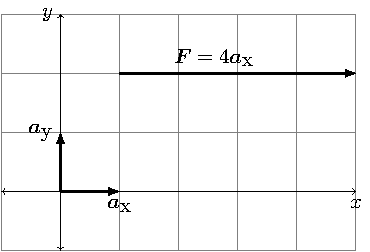
\includegraphics{figBasicFactsUnitVectors}
\begin{tikzpicture}
\draw[help lines] (-1,-1) grid (5,3);
\draw[thin, <->] (-1,0)--(5,0) node[below,black]{$x$};
\draw[thin, <->] (0,-1)--(0,3) node[left,black]{$y$};
\draw[thick,-latex] (0,0)--(1,0) node[below] {$\ax$};
\draw[thick,-latex] (0,0)--(0,1) node[left] {$\ay$};

\draw[thick,-latex](1,2)--(5,2)node[pos=0.4,above] {$\kvec{F}=4 \ax$};
\end{tikzpicture}%
\caption{کارتیسی محدد}
\label{شکل_حقائق_اکائی_سمتیہ}
\end{figure}
%
\حصہ{محدد}
ایسا طریقہ جس کے ذریعہ کسی نقطہ کا مقام متعین کیا جا سکے محدد کہلاتا ہے۔

خلاء  تین بعدی (تین طرفہ) \حاشیہب{three dimensional} ہے لہٰذا  کسی ایک نقطہ کے مقام کو تین محدد کی مدد سے ظاہر کیا جا سکتا ہے۔اسی طرح  خلاء میں سمتیہ کو تین عمودی اکائی سمتیوں کی مدد سے لکھا جا سکتا ہے۔اب ہم ایسے چند محدد کے نظام دیکھتے ہیں۔

\جزوحصہ{کارتیسی محددی نظام}
شکل \حوالہ{شکل_حقائق_اکائی_سمتیہ}   میں خلاء کی دو سمتوں کو  اکائی سمتیات \عددیء{\ax} اور \عددیء{\ay} سے ظاہر کیا گیا ہے جو آپس میں عمودی ہیں، یعنی، ان کے بیچ \عددیء{90\degree}  زاویہ ہے۔خلاء تین بعدی ہے لہٰذا اسے تین آپس میں \اصطلاح{عمودی اکائی سمتیات}\فرہنگ{سمتیہ!عمودی اکائی}\حاشیہب{orthonormal vectors}\فرہنگ{orthonormal} سے ظاہر کیا جاتا ہے۔ ان سمتوں کے رخ،  طول (لمبائیوں)  کو \عددیء{x,y,z} سے ظاہر کیا جاتا ہے۔ آپ ان سے بخوبی واقف ہیں۔ 

 دائیں ہاتھ کا انگوٹھا، شہادت کی انگلی اور  بڑی انگلی کو ایک دوسرے کے ساتھ \عددی{90^{\circ}} زاویہ پر رکھتے ہوئے اگر شہادت کی انگلی \عددی{\ax} اور بڑی انگلی \عددی{\ay} کے رخ ہوں تب انگوٹھا \عددی{\az} کے رخ ہو گا (شکل \حوالہ{شکل_حقائق_دائیں_ہاتھ})۔ اسی لئے  تین اکائی سمتیات کا یہ نظام \اصطلاح{دائیں ہاتھ کا نظام}\حاشیہب{right handed coordinate system}  کہلاتا ہے۔

\begin{figure}
\centering
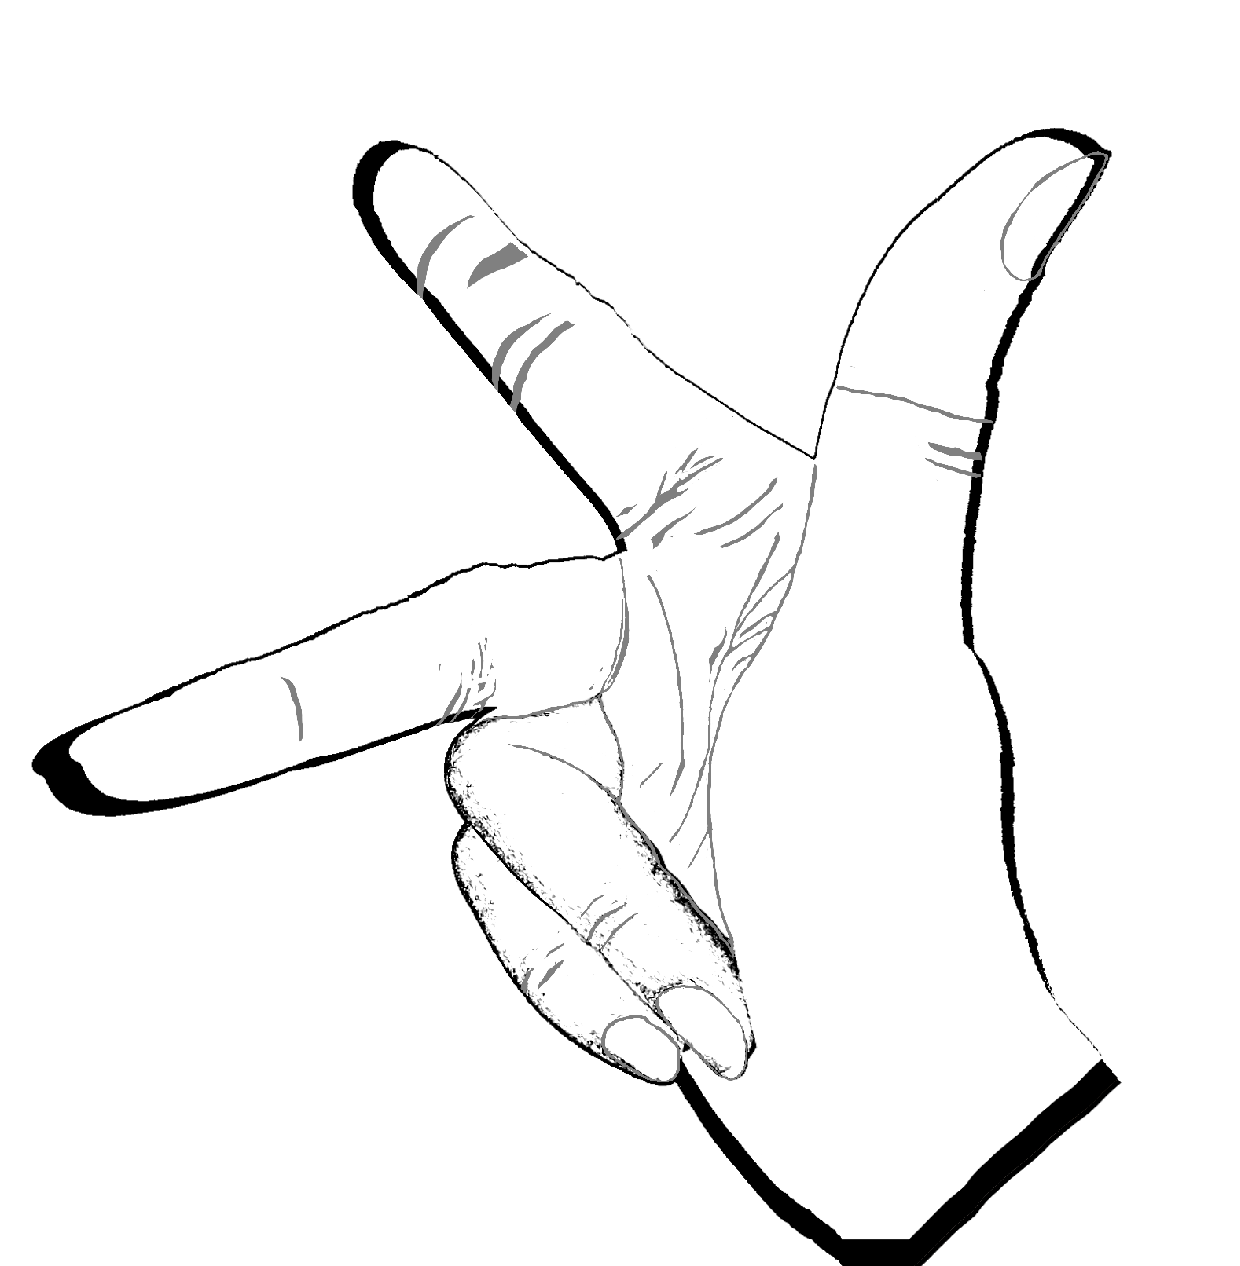
\includegraphics[height=3.5cm]{figRightHandRule}
\caption{دائیں ہاتھ کا نظام۔}
\label{شکل_حقائق_دائیں_ہاتھ}
\end{figure}
مبدا سے نقطہ \عددی{P(x,y,z)} تک سمتیہ \سمتیہ{A} کو شکل \حوالہ{شکل_حقائق_کارتیسی_نظام_ایک_سمتیہ} میں دکھایا  گیا ہے جس کو \اصطلاح{کارتیسی محدد}\فرہنگ{محدد!کارتیسی}\فرہنگ{cartesian system}\حاشیہب{cartesian coordinates} میں تین سمتیات کی مدد سے
\begin{align}
\kvec{A}=\kvec{A}_x+\kvec{A}_y+\kvec{A}_z
\end{align}
یا
\begin{align}
\kvec{A}=x\ax+y\ay+z\az
\end{align}
لکھا جا سکتا ہے۔
%
\begin{figure}
\centering
%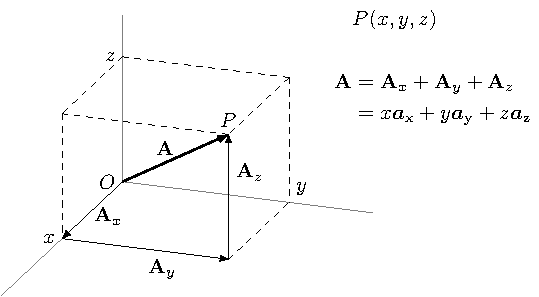
\includegraphics{figBasicFactsVectorCartesianCoordinates}
\tdplotsetmaincoords{70}{110}
\begin{tikzpicture}[scale=3,tdplot_main_coords]
\def\kkkx{1}
\def\kkky{1}
\def\kkkz{0.75}
\coordinate (O) at (0,0,0);
\coordinate (P) at (\kkkx,\kkky,\kkkz);
%axis
\draw[gray] (0,0,0) -- (2,0,0);
\draw[gray] (0,0,0) -- (0,1.5,0);
\draw[gray] (0,0,0) -- (0,0,1);
%equations
\node[anchor=east] at (0,2.5,1) {$\begin{aligned}
& P(x,y,z)\\
\\
\bf{A}&={\bf{A}}_x+{\bf{A}}_y+{\bf{A}}_z\\
&=x \ax+y \ay+z \az
     \end{aligned}$};
%text
\node[anchor=east] at (\kkkx,0,0) {$x$};
\node[anchor=south west] at (0,\kkky,0) {$y$};
\node[anchor=east] at (0,0,\kkkz) {$z$};
\node[anchor=east] at (0,0,0) {$O$};
\node[anchor=south] at (\kkkx,\kkky,\kkkz) {$P$};

%dashed
\draw[dashed] (\kkkx,\kkky,\kkkz)--(\kkkx,0,\kkkz);
\draw[dashed] (\kkkx,0,\kkkz)--(\kkkx,0,0);

\draw[dashed] (\kkkx,\kkky,0)--(0,\kkky,0);
\draw[dashed] (0,\kkky,\kkkz)--(\kkkx,\kkky,\kkkz);
\draw[dashed] (0,\kkky,\kkkz)--(0,\kkky,0);

\draw[dashed] (0,\kkky,\kkkz)--(0,0,\kkkz);
\draw[dashed] (0,0,\kkkz)--(\kkkx,0,\kkkz);
%vectors
\draw[thick,-latex] (0,0,0)--(\kkkx,\kkky,\kkkz) node[pos=0.4, above]{$\bf{A}$};
\draw[thin,-latex] (0,0,0)--(\kkkx,0,0) node[pos=0.6, right]{${\bf{A}}_x$};
\draw[thin,-latex] (\kkkx,0,0)--(\kkkx,\kkky,0)  node[pos=0.6, below]{${\bf{A}}_y$};
\draw[thin,-latex] (\kkkx,\kkky,0)--(\kkkx,\kkky,\kkkz)  node[pos=0.7, right]{${\bf{A}}_z$};
%
%\draw[gray,-latex](O)--(N1)node[pos=0.4, right]{$\bf{r_1}$} node[below,black]{$Q_1$};
%\draw[gray,-latex](O)--(N2)node[pos=0.4,right]{$\bf{r_2}$} node[above,black]{$Q_2$};
%\draw[gray,-latex](O)--(N)node[pos=0.4,above]{$\bf{r_N}$};
%
%\draw[thin, gray,-latex](N1)--(N);
%\draw[shorten <=2.3cm,shorten >=-.5cm,-latex](N1) --(N);
%\draw[thin, gray,-latex](N2)--(N);
%\draw[shorten <=3.1cm,shorten >=-.5cm,-latex](N2)--(N);

%\draw[blue](current bounding box.south west) rectangle (current bounding box.north east);
%\draw[help lines, step=10pt](0,0)grid(1,1);
%\path[use as bounding box]( -1.2,-1.5,-1)rectangle(1,2,2);
\end{tikzpicture}%

\caption{کارتیسی محدد نظام میں ایک سمتیہ۔}
\label{شکل_حقائق_کارتیسی_نظام_ایک_سمتیہ}
\end{figure}

کارتیسی محددی نظام میں متغیر \عددی{z}  صفر رکھتے ہوئے \عددیء{x,y} تبدیل کرنے سے  سطح \عددی{xy} ملتی ہے۔ یوں  شکل \حوالہ{شکل_حقائق_کارتیسی_نظام_ایک_سمتیہ}  میں \عددی{P(2,4,3)} لے کر، سطح \عددیء{xy} کو زمین تصور کرتے  ہوئے،  ڈبے کی بالائی سطح پر   \عددیء{z=3} جبکہ \عددی{x} کی قیمت صفر تا  تین اور \عددی{y} کی قیمت صفر تا چار ہو گی۔ اس طرح اس ڈبے کی بالائی سطح درج ذیل لکھی جائے گی۔
\begin{align}
 \text{\RL{ڈبے کی بالائی سطح}}= 
\begin{cases}
    0<x<2\\
    0<y<4 \\
	 z=3
  \end{cases}
\end{align}

متغیر \عددیء{z} کو صفر اور تین کے درمیان ہر ممکن قیمت پر رکھ کر \عددی{x} کو صفر اور دو جبکہ \عددی{y} کو صفر اور چار کے درمیان تبدیل کرنے سے شکل \حوالہ{شکل_حقائق_کارتیسی_نظام_ایک_سمتیہ} میں دکھائے گئے ڈبے کا حجم حاصل ہو گا، لہٰذا اس ڈبے کا حجم درج ذیل لکھا جائے گا۔
\begin{align}
 \text{\RL{ڈبے کا حجم}}=
\begin{cases}
    0<x<2\\
    0<y<4 \\
    0<z<3
  \end{cases}
\end{align}

\جزوحصہ{نلکی محددی نظام}
مبدا سے نقطہ \عددیء{P(x,y,z)} تک  سمتیہ  \سمتیہ{A} کو شکل \حوالہ{شکل_حقائق_نلکی_نظام_ایک_سمتیہ}  میں دکھایا گیا ہے جس  کو دو سمتیات کی مدد سے
\begin{align}
\kvec{A}=\kvec{\rho}+\kvec{A}_z
\end{align}
یا
\begin{align}
\kvec{A}=\rho \arho+z \az
\end{align}
لکھا جا سکتا ہے۔
%
\begin{figure}
\centering
%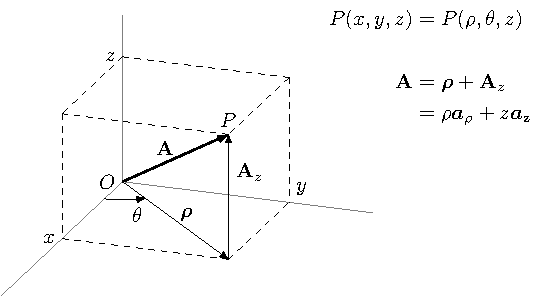
\includegraphics{figBasicFactsVectorCylindricalCoordinates}
\tdplotsetmaincoords{70}{110}
\begin{tikzpicture}[scale=3,tdplot_main_coords]
\def\kkkx{1}
\def\kkky{1}
\def\kkkz{0.75}
\coordinate (O) at (0,0,0);
\coordinate (P) at (\kkkx,\kkky,\kkkz);
%axis
\draw[gray] (0,0,0) -- (2,0,0);
\draw[gray] (0,0,0) -- (0,1.5,0);
\draw[gray] (0,0,0) -- (0,0,1);
%equations
\node[anchor=east] at (0,2.5,1) {$\begin{aligned}
P(x,y,z)&=P(\rho,\theta,z)\\
\\
\bf{A}&={\kvec{\rho}}+{\bf{A}}_z\\
&=\rho \arho+z \az
     \end{aligned}$};
%text
\node[anchor=east] at (\kkkx,0,0) {$x$};
\node[anchor=south west] at (0,\kkky,0) {$y$};
\node[anchor=east] at (0,0,\kkkz) {$z$};
\node[anchor=east] at (0,0,0) {$O$};
\node[anchor=south] at (\kkkx,\kkky,\kkkz) {$P$};

%dashed
\draw[dashed] (\kkkx,0,0)--(\kkkx,\kkky,0);
\draw[dashed] (\kkkx,\kkky,\kkkz)--(\kkkx,0,\kkkz);
\draw[dashed] (\kkkx,0,\kkkz)--(\kkkx,0,0);

\draw[dashed] (\kkkx,\kkky,0)--(0,\kkky,0);
\draw[dashed] (0,\kkky,\kkkz)--(\kkkx,\kkky,\kkkz);
\draw[dashed] (0,\kkky,\kkkz)--(0,\kkky,0);

\draw[dashed] (0,\kkky,\kkkz)--(0,0,\kkkz);
\draw[dashed] (0,0,\kkkz)--(\kkkx,0,\kkkz);
%vectors
\draw[thick,-latex] (0,0,0)--(\kkkx,\kkky,\kkkz) node[pos=0.4, above]{$\bf{A}$};
\draw[thin,-latex] (0,0,0)--(\kkkx,\kkky,0)  node[pos=0.6, above]{${\kvec{\rho}}$};
\draw[thin,-latex] (\kkkx,\kkky,0)--(\kkkx,\kkky,\kkkz)  node[pos=0.7, right]{${\bf{A}}_z$};
%arc
 \tdplotdrawarc[color=black,-latex,tdplot_main_coords]{(0,0,0)}{0.3}{0}{45}{anchor=north west}{$\theta$};
\end{tikzpicture}%
\caption{نلکی محددی نظام}
\label{شکل_حقائق_نلکی_نظام_ایک_سمتیہ}
\end{figure}
سمتیہ $\arho$ سطح \عددی{xy} میں پایا جاتا ہے۔ شکل \حوالہ{شکل_حقائق_نلکی_نظام_ایک_سمتیہ} کو دیکھتے ہوئے
\begin{align*}
x=\rho \cos \theta,\quad y=\rho \sin \theta
\end{align*}
لکھ کر نقطہ \عددی{P(x,y,z)} کو متغیرات \عددیء{x,y,z} کے بجائے متغیرات \عددیء{\rho,\theta,z} کی مدد سے \عددیء{P(\rho,\theta,z)} لکھا جا سکتا ہے۔ یوں خلاء میں کسی بھی نقطہ کو اس کے تین متغیرات \عددیء{\rho,\theta,z} سے ظاہر کیا جا سکتا ہے۔

وہ نظام جس میں متغیرات \عددیء{\rho,\theta,z}  کسی نقطہ کو متعین کرتے  ہوں  \اصطلاح{نلکی محدد}\فرہنگ{محدد!نلکی}\حاشیہب{cylindrical coordinates}\فرہنگ{cylindrical coordinates} کہلاتا ہے۔یہاں شکل \حوالہ{شکل_حقائق_نلکی_نظام_تعریف}  سے رجوع کریں۔ نلکی محددی نظام کے تین آپس میں عمودی  اکائی سمتیات $\arho,\atheta,\az$ ہیں۔ یہ نظام بھی دائیں ہاتھ کا نظام ہے لہٰذا دائیں ہاتھ کا انگوٹھا، شہادت کی انگلی اور  بڑی انگلی کو ایک دوسرے کے ساتھ \عددی{90^{\circ}} پر رکھتے ہوئے اگر  شہادت کی انگلی \عددی{\arho} اور بڑی انگلی \عددی{\atheta} کے رخ ہوں تب انگوٹھا \عددی{\az} کے رخ ہو گا۔ 

سطح \عددی{xy} میں مبدا پر، محدد \عددی{x} کے ساتھ  \عددی{\theta} زاویہ پر اکائی سمتیہ  $\arho$ ہو گا۔  سطح  \عددیء{xy} میں مبدا پر اکائی سمتیہ $\arho$ کے عمودی، بڑھتے  \عددی{\theta} رخ، اکائی   سمتیہ $\atheta$ ہو گا۔ کارتیسی محددی نظام کا اکائی سمتتیہ $\az$ ہی نلکی محدد کا اکائی سمتیہ $\az$ ہے۔ 
\begin{figure}
\centering
%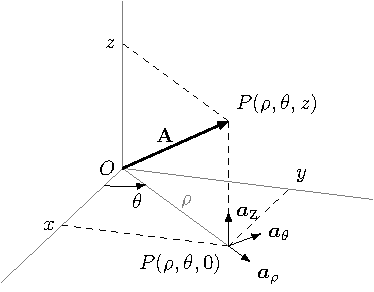
\includegraphics[height=3.5cm]{figBasicFactsCylindricalCoordinates}
\tdplotsetmaincoords{70}{110}
\begin{tikzpicture}[scale=3,tdplot_main_coords]
\def\kkkx{1}
\def\kkky{1}
\def\kkkz{0.75}
\coordinate (O) at (0,0,0);
\coordinate (P) at (\kkkx,\kkky,\kkkz);
%axis
\draw[gray] (0,0,0) -- (2,0,0);
\draw[gray] (0,0,0) -- (0,1.5,0);
\draw[gray] (0,0,0) -- (0,0,1);

%text
\node[anchor=east] at (\kkkx,0,0) {$x$};
\node[anchor=south west] at (0,\kkky,0) {$y$};
\node[anchor=east] at (0,0,\kkkz) {$z$};
\node[anchor=east] at (0,0,0) {$O$};
\node[anchor=south west] at (\kkkx,\kkky,\kkkz) {$P(\rho,\theta,z)$};
\node[anchor=north east]  at (\kkkx,\kkky,0) {$P(\rho,\theta,0)$};

%dashed
\draw[dashed] (\kkkx,0,0)--(\kkkx,\kkky,0);
\draw[dashed] (\kkkx,\kkky,\kkkz)--(\kkkx,\kkky,0);
\draw[dashed] (\kkkx,\kkky,\kkkz)--(0,0,\kkkz);
\draw[dashed] (\kkkx,\kkky,0)--(0,\kkky,0);

%\draw[dashed] (0,\kkky,\kkkz)--(\kkkx,\kkky,\kkkz);
%\draw[dashed] (0,\kkky,\kkkz)--(0,\kkky,0);

%\draw[dashed] (0,\kkky,\kkkz)--(0,0,\kkkz);
%\draw[dashed] (0,0,\kkkz)--(\kkkx,0,\kkkz);
%vectors
\draw[thin,gray] (0,0,0)--(\kkkx,\kkky,0)  node[pos=0.6, above]{${\rho}$};
\draw[thick,-latex] (0,0,0)--(\kkkx,\kkky,\kkkz) node[pos=0.4, above]{$\bf{A}$};
%\draw[thin,-latex] (0,0,0)--(\kkkx,0,0) node[pos=0.6, right]{${\bf{A}}_x$};
%\draw[thin,-latex] (\kkkx,0,0)--(\kkkx,\kkky,0)  node[pos=0.6, below]{${\bf{A}}_y$};

%unit vectors
\draw[thin,-latex] (\kkkx,\kkky,0)--(1.2*\kkkx,1.2*\kkky,0)  node[below right]{${\arho}$};
\draw[thin,-latex] (\kkkx,\kkky,0)--(0.75*\kkkx,1.1*\kkky,0)  node[right]{${\atheta}$};
\draw[thin,-latex] (\kkkx,\kkky,0)--(\kkkx,\kkky,0.2)  node[right]{${\az}$};
%\draw[thin,-latex] (\kkkx,\kkky,0)--(\kkkx,\kkky,\kkkz)  node[pos=0.7, right]{${\bf{A}}_z$};

%arc
 \tdplotdrawarc[color=black,-latex,tdplot_main_coords]{(0,0,0)}{0.3}{0}{45}{anchor=north west}{$\theta$};
\end{tikzpicture}%
\caption{نلکی نما محدد کی تعریف}
\label{شکل_حقائق_نلکی_نظام_تعریف}
\end{figure}

واضح رہے کہ  نلکی محدد کے نظام  میں $\arho$ اور  $\atheta$ کی سمتیں ہر نقطہ پر مختلف ہیں جیسا کہ شکل \حوالہ{شکل_حقائق_نلکی_نظام_میں_اکائی_سمتیات_اٹل_نہیں} میں دکھایا گیا ہے۔
\begin{figure}
\centering
%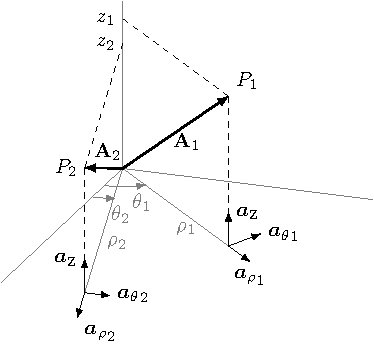
\includegraphics[height=3.5cm]{figBasicFactsCylindricalCoordinatesVaryingUnitVectors}
\tdplotsetmaincoords{70}{110}
\begin{tikzpicture}[scale=3,tdplot_main_coords]
\def\kkkx{1}
\def\kkky{1}
\def\kkkz{0.9}
\def\kkx{2}
\def\kky{0.5}
\def\kkz{0.75}
\coordinate (O) at (0,0,0);
\coordinate (P) at (\kkkx,\kkky,\kkkz);
\coordinate (PP) at (\kkx,\kky,\kkz);
%axis
\draw[gray] (0,0,0) -- (2,0,0);
\draw[gray] (0,0,0) -- (0,1.5,0);
\draw[gray] (0,0,0) -- (0,0,1);

%text

\node[anchor=south west] at (\kkkx,\kkky,\kkkz) {$P_1$};
\node[anchor= east]  at (\kkx,\kky,\kkz) {$P_2$};

%dashed
\draw[dashed] (\kkkx,\kkky,\kkkz)--(\kkkx,\kkky,0);
\draw[dashed] (\kkkx,\kkky,\kkkz)--(0,0,\kkkz) node[left] {$z_1$};

\draw[dashed] (\kkx,\kky,\kkz)--(\kkx,\kky,0);
\draw[dashed] (\kkx,\kky,\kkz)--(0,0,\kkz)node[left] {$z_2$};

%vectors
\draw[thin,gray] (0,0,0)--(\kkkx,\kkky,0)  node[pos=0.6, below]{${\rho_1}$};
\draw[thick,-latex] (0,0,0)--(\kkkx,\kkky,\kkkz) node[pos=0.6, below]{${\bf{A}}_1$};

\draw[thin,gray] (0,0,0)--(\kkx,\kky,0)  node[pos=0.6, right]{${\rho_2}$};
\draw[thick,-latex] (0,0,0)--(\kkx,\kky,\kkz) node[pos=0.4, above]{${\bf{A}}_2$};


%unit vectors
\draw[thin,-latex] (\kkkx,\kkky,0)--(1.2*\kkkx,1.2*\kkky,0)  node[ below]{${\arho}_1$};
\draw[thin,-latex] (\kkkx,\kkky,0)--(0.75*\kkkx,1.1*\kkky,0)  node[right]{${\atheta}_1$};
\draw[thin,-latex] (\kkkx,\kkky,0)--(\kkkx,\kkky,0.2)  node[right]{${\az}$};

\draw[thin,-latex] (\kkx,\kky,0)--(1.2*\kkx,1.2*\kky,0)  node[below right]{${\arho}_2$};
\draw[thin,-latex] (\kkx,\kky,0)--(\kkx,1.3*\kky,0)  node[right]{${\atheta}_2$};
\draw[thin,-latex] (\kkx,\kky,0)--(\kkx,\kky,0.2)  node[left]{${\az}$};
%\draw[thin,-latex] (\kkkx,\kkky,0)--(\kkkx,\kkky,\kkkz)  node[pos=0.7, right]{${\bf{A}}_z$};
%arc
 \tdplotdrawarc[color=gray,-latex,tdplot_main_coords]{(0,0,0)}{0.3}{0}{45}{anchor=north west}{$\theta_1$};
\tdplotdrawarc[color=gray,-latex,tdplot_main_coords]{(0,0,0)}{0.5}{0}{15}{anchor=north west}{$\theta_2$};
\end{tikzpicture}
\caption{نلکی محدد میں اکائی سمتیات \عددیء{\arho} اور \عددیء{\atheta} ہر نقطہ پر مختلف ہیں۔}
\label{شکل_حقائق_نلکی_نظام_میں_اکائی_سمتیات_اٹل_نہیں}
\end{figure}

مستوی \عددی{xy} میں (یعنی \عددی{z=0} لیتے ہوئے) مبدا پر مستقل رداس \عددی{\rho=\rho_0}   کے سمتیہ کو صفر زاویہ پر رکھ کر زاویہ  بتدریج \عددی{2\pi} تک بڑھانے سے سمتیہ کی چونچ مستوی \عددی{xy} میں ایک دائرہ پر چلتی ہے (شکل \حوالہ{شکل_حقائق_نلکی_نظام_میں_دائرہ_اور_نلکی})۔ اب اس سمتیہ کے متغیر \عددی{z} کو تبدیل کرنے سے، مثلاً ہر \عددی{\theta} پر \عددیء{z} کو صفر تا تین کرنے سے، یہ سمتیہ ایک نلکی بنائے گی۔ اسی وجہ سے اس نظام کو نلکی محدد کہتے ہیں۔ سمتیہ کے تینوں متغیرہ تبدیل کرنے سے   نلکی کا حجم ملے گا۔ اگلی تین مساوات ان حقائق کو پیش کرتی ہیں۔
\begin{align}
 \text{دائرہ}&=\begin{cases} 
    \rho=\rho_0\\
    0<\theta<2 \pi \\
    z=0 
\end{cases}\\
 \text{\RL{نلکی نما سطح}}&= \begin{cases}
    \rho=\rho_0\\
    0<\theta<2 \pi \\
  0<z<z_0
  \end{cases}\\
 \text{\RL{نلکی کا حجم}}&= \begin{cases}
    0<\rho<\rho_0\\
    0<\theta<2 \pi \\
  0<z<z_0
  \end{cases}
\end{align}
%
\begin{figure}
\centering
%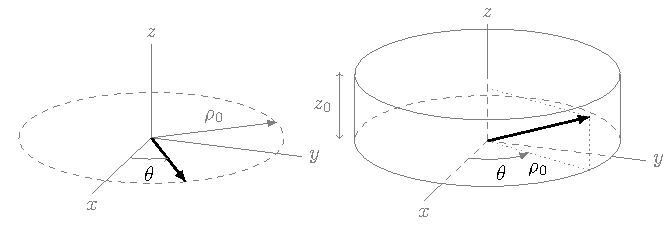
\includegraphics[height=2.5cm]{figBasicFactsCylindricalCoordinatesCircleAndCylinder}
\tdplotsetmaincoords{70}{110}
\begin{tikzpicture}[scale=3,tdplot_main_coords]
%CIRCLE
\coordinate (O) at (0,0,0);
\def\angleA{35};
\def\angleB{130};
\def\kradius{0.75};
\def\height{0.4};
%axis
\draw[gray] (0,0,0) -- (1.3*\kradius,0,0) node[below] {$x$};
\draw[gray] (0,0,0) -- (0,1.2*\kradius,0) node[right] {$y$};
\draw[gray] (0,0,0) -- (0,0,0.75*\kradius) node[above] {$z$};

%circle
\tdplotdrawarc[gray, dashed]{(O)}{\kradius}{0}{360}{}{};
%vectors
\tdplotsinandcos{\sintheta}{\costheta}{\angleA}%
\draw[thick,-latex] (0,0,0)--(\kradius * \costheta,\kradius * \sintheta,0);
\tdplotsinandcos{\sintheta}{\costheta}{\angleB}%
\draw[gray,-latex] (0,0,0)--(\kradius * \costheta,\kradius * \sintheta,0)  node[pos=0.5, above]{${\rho_0}$};
%text
\tdplotdrawarc[gray,->]{(0,0,0)}{0.35}{0}{\angleA}{anchor=north,color=black}{$\theta$};

%CYLINDER
%axis for cylinder
\def\movey{1.8};
\def\movex{-0.6};
\coordinate (Oc) at (\movex,\movey,0);
\coordinate (Occ) at (\movex,\movey,\height);

\draw[gray,dashed] (Oc) -- ++(\kradius,0,0);  %hidden axis
\draw[gray,dashed] (Oc) -- ++(0,\kradius,0);
\draw[gray,dashed] (Oc) -- ++(0,0,\height);

\draw[gray] (Oc)++(\kradius,0,0) -- ++(0.3,0,0)node[below ] {$x$};  %visible axis
\draw[gray] (Oc)++(0,\kradius,0) -- ++(0,0.2,0)node[right ] {$y$};
\draw[gray] (Oc)++(0,0,\height) -- ++(0,0,0.3)node[above] {$z$};

%top and bottom of cylinder
\tdplotdrawarc[gray, dashed]{(Oc)}{\kradius}{110}{290}{}{};   %bottom of cylinder
\tdplotdrawarc[gray]{(Oc)}{\kradius}{-70}{110}{}{};
\tdplotdrawarc[gray]{(Occ)}{\kradius}{0}{360}{}{};   %top of cylinder
%left edge of cylinder
\tdplotsinandcos{\sintheta}{\costheta}{-70}%
\coordinate (leftLower) at (\movex+\kradius * \costheta,\movey+\kradius * \sintheta, 0);
\coordinate (leftUpper) at (\movex+\kradius * \costheta,\movey+\kradius * \sintheta, \height);
\draw[gray](leftLower)--(leftUpper);
%showing height
\coordinate (leftLowerL) at (\movex+\kradius * \costheta,0.95*\movey+\kradius * \sintheta, 0);
\coordinate (leftUpperL) at (\movex+\kradius * \costheta,0.95*\movey+\kradius * \sintheta, \height);
\draw[gray,<->](leftLowerL)--(leftUpperL) node[pos=0.5,left]{$z_0$};

%right edge of cylinder
\tdplotsinandcos{\sintheta}{\costheta}{110}%
\coordinate (rightLower) at (\movex+\kradius * \costheta,\movey+\kradius * \sintheta, 0);
\coordinate (rightUpper) at (\movex+\kradius * \costheta,\movey+\kradius * \sintheta, \height);
\draw[gray](rightLower)--(rightUpper);
%vector
\tdplotsinandcos{\sintheta}{\costheta}{70}%
\draw[thick,-latex](Oc)--++(\kradius * \costheta,\kradius * \sintheta, 0.8*\height); %main vector
\draw[gray,dotted](Oc)--++(\kradius * \costheta,\kradius * \sintheta, 0)node[pos=0.5,black,below] {$\rho_0$}; %vector horizontal section lower
\draw[gray,dotted](Oc)++(0,0,0.8*\height) --++(\kradius * \costheta,\kradius * \sintheta,0); %vector horizontal section upper
\draw[gray,dotted](Oc)++(\kradius * \costheta,\kradius * \sintheta, 0)--++(0,0,0.8*\height); %vector vertical section
%showing angle
 \tdplotdrawarc[color=gray,-latex,tdplot_main_coords]{(Oc)}{0.3}{0}{70}{anchor=north,black}{$\theta$};
%\tdplotdrawarc[color=gray,-latex,tdplot_main_coords]{(0,0,0)}{0.5}{0}{15}{anchor=north west}{$\theta_2$};

\end{tikzpicture}%

\caption{‫نلکی محدد میں دائرہ اور نلکی‬}
\label{شکل_حقائق_نلکی_نظام_میں_دائرہ_اور_نلکی}
\end{figure}

\حصہ{سمتیہ رقبہ}
سطح پر کھڑا  اکائی سمتیہ سطح کا رخ دیتا ہے (شکل \حوالہ{شکل_حقائق_رقبہ_سمتیہ})۔  چونکہ کسی بھی سطح  کے دو اطراف ہوتے ہیں لہٰذا اس کے دو مخالف  رخ بیان کیے جا سکتے ہیں۔عموماً مسئلہ کو مدِ نظر رکھتے ہوئے  ان میں سے ایک رخ  کو سطح کا رخ  تصور کیا جاتا ہے۔ البتہ بند سطح، مثلاً  گیند، کے بیرونی رخ کو ہی سطح کا رخ تصور کیا جاتا ہے۔شکل \حوالہ{شکل_حقائق_رقبہ_سمتیہ} میں بالائی  سطح \سمتیہ{A_1}  کا رقبہ \عددیء{A_1} ہے اور اس کا رخ $\az$ ہے لہٰذا  \سمتیہ{A_1} سمتیہ کا طول  \عددیء{A_1}  اور رخ $\az$ ہو گا:
\begin{figure}
\centering
%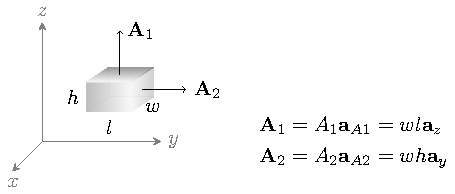
\includegraphics[height=2.5cm]{figBasicFactsVectorArea}
\begin{tikzpicture}
\pgfmathsetmacro{\xst}{0.75}            %start points, lower left corner
 \pgfmathsetmacro{\yst}{0.5}
 \pgfmathsetmacro{\xdel}{0.75}           %change from start point
 \pgfmathsetmacro{\ydel}{0.5}
%front of cube
\coordinate (n1) at (\xst,\yst);
\coordinate (n2) at (\xst+\xdel,\yst);
\coordinate (n3) at (\xst+\xdel,\yst+\ydel);
\coordinate (n4) at (\xst,\yst+\ydel);
%back of cube
\coordinate (n5) at (\xst+0.5*\xdel,\yst+0.5*\ydel);
\coordinate (n6) at (\xst+1.5*\xdel,\yst+0.5*\ydel);
\coordinate (n7) at (\xst+1.5*\xdel,\yst+1.5*\ydel);
\coordinate (n8) at (\xst+0.5*\xdel,\yst+1.5*\ydel);
%
%face's centres
\coordinate (fr) at (\xst+1.25*\xdel,\yst+0.75*\ydel); %right face
\coordinate (ft) at (\xst+0.75*\xdel,\yst+1.25*\ydel); %right face
%axis
\draw[-stealth,gray] (0,0)--(2,0) node[right]{$y$};
\draw[-stealth,gray] (0,0)--(0,2) node[above]{$z$};
\draw[-stealth,gray] (0,0)--(-0.5,-0.5) node[below]{$x$};

%point charge at centre of cube
%\draw[fill] (\xst+0.75*\xdel,\yst+0.75*\ydel) circle (0.2mm);
%flux density
%\node[right] at (1.75,1.75) {${\bf{D}}(x_0,y_0,z_0)=D_{x0}{\bf{a}}_x+D_{y0} {\bf{a}}_y+D_{z0} {\bf{a}}_z$};
%\draw[-stealth] (1.75,1.75) to [out=180,in=90] (\xst+0.75*\xdel,\yst+0.75*\ydel);
%back edges of cube
\draw[very thin,gray!10] (n5)--(n6);
\draw[very thin,gray!10] (n5)--(n1);
\draw[very thin,gray!10] (n5)--(n8);
%front,right and top of cube
\shade[opacity=0.5,right color=gray!10, left color=black!50] (n1)--(n2) --(n3)--(n4)--cycle;
\shade[opacity=0.5,right color=gray!70,left color=gray!10] (n2)--(n6)--(n7)--(n3)--cycle;
\shade[opacity=0.5,bottom color=gray!10, top color=black!80] (n4)--(n3)--(n7)--(n8)--cycle;

\path (n2)--(n6) node [black,right,pos=0.3]{$w$};
\path (n1)--(n2) node[black,below,pos=0.5]{$l$};
\path (n1)--(n4) node [black,left,pos=0.5]{$h$};

%--top and right face vectors
\draw[->] (fr)--++(1*\xdel,0) node [right] {${\bf{A}}_2$};
\draw[->] (ft)--++(0,1.5*\ydel) node [right] {${\bf{A}}_1$};
%aligned equations
\node[anchor=east] at (7,0){$
\begin{aligned}
{\bf{A}}_1&=A_1 {\bf{a}}_{A1}=w l {\bf{a}}_z\\
{\bf{A}}_2&=A_2 {\bf{a}}_{A2}=w h {\bf{a}}_y
\end{aligned}$
};
\end{tikzpicture}
\caption{سمتیہ رقبہ کا تعارف‬}
\label{شکل_حقائق_رقبہ_سمتیہ}
\end{figure}
%
\begin{align*}
A_1&=wl\\
\kvec{a_{A1}}&=\az
\end{align*}
یوں بالائی سطح کا سمتی رقبہ درج ذیل ہو گا۔
\begin{align}
\kvec{A_1}=A_1 \kvec{a_{A1}}= w l \az
\end{align}
اسی طرح دائیں  سطح \سمتیہ{A_2} سمتیہ  کا طول \عددیء{A_2}  اور اس کا رخ \سمتیہ{a_{A2}} ہے
\begin{align*}
A_2=wh\\
\kvec{a_{A2}}=\ay
\end{align*}
لہٰذا درج ذیل ہو گا۔
\begin{align}
\kvec{A_2}=A_2 \kvec{a_{A1}}=w h \ay
\end{align}
نچلی سطح کا رقبہ \عددیء{A_3=wl}  اور اس کا رخ  $\az$ کے مخالف  ہے لہٰذا درج ذیل ہو گا۔
\begin{align}
\kvec{A_3}=A_3 \kvec{a_{A3}}=wl (-\az)=-wl \az
\end{align}
دھیان  رہے کہ رقبہ کی مقدار ہر صورت  مثبت ہو گی البتہ اس کا رخ مثبت یا منفی ہو سکتا ہے۔ یہ بات کسی بھی سمتیہ کے لئے درست ہے لہٰذا کسی بھی سمتیہ کا طول ہر صورت  مثبت ہی ہو گا جبکہ  اس کا رخ  مثبت یا منفی ہو سکتا  ہے۔

\حصہ{رقبہ عمودی تراش}
سلاخ  کی لمبائی کے ساتھ زاویہ قائمہ  پر  کٹائی کو \اصطلاح{عمودی تراش}\فرہنگ{عمودی تراش}\حاشیہب{cross section}\فرہنگ{cross section} کہتے ہیں اور عمودی تراش کے رقبہ کو \اصطلاح{رقبہ عمودی تراش}\فرہنگ{عمودی تراش!رقبہ}\حاشیہب{cross sectional area} کہتے ہیں۔شکل \حوالہ{شکل_حقائق_رقبہ_عمودی}  میں  سلاخ کی لمبائی   $\ay$  رخ  ہے اور  رقبہ عمودی تراش \سمتیہ{A} کی مقدار \عددیء{A} ہے
\begin{align}
A=wh
\end{align}
لہٰذا رقبہ عمودی تراش کا رخ  $\ay$  ہو گا:
\begin{align}
\kvec{a_A}=\ay
\end{align}
شکل \حوالہ{شکل_حقائق_رقبہ_عمودی}  میں  اکائی سمتیات  $\ay$  اور  $\az$ دکھائے گئے ہیں جن کے ابتدائی نقاط پر گول دائرہ میں بند ایک نقطہ دکھایا گیا ہے۔گول دائرہ میں بند نقطہ صفحہ کے عمودی (کتاب سے باہر)  رخ  $\ax$ ظاہر کرتا ہے جس کے مخالف رخ  (صفحہ کے عمودی اندر)  کو گول دائرہ میں بند صلیب کی نشان سے ظاہر کیا جائے گا۔
%
\begin{figure}
\centering
%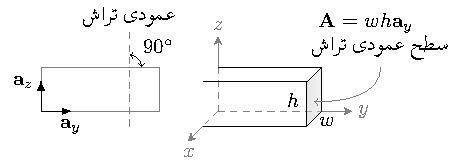
\includegraphics[height=2.5cm]{figBasicFactsCrossSectionalArea}
\begin{tikzpicture}
\pgfmathsetmacro{\xst}{0.75}            %start points, lower left corner
 \pgfmathsetmacro{\yst}{0.5}
 \pgfmathsetmacro{\xdel}{0.75}           %change from start point
 \pgfmathsetmacro{\ydel}{0.5}
\coordinate(O) at (3,0,0);
%front of cube
\coordinate (n1) at (\xst,\yst);
\coordinate (n2) at (\xst+\xdel,\yst);
\coordinate (n3) at (\xst+\xdel,\yst+\ydel);
\coordinate (n4) at (\xst,\yst+\ydel);
%side view
\draw[gray](0,0,0)--(2,0,0)--(2,0.75,0)--(0,0.75,0)--cycle;
\draw[gray,dashed](1.5,-0.25,0)--(1.5,1.4,0);
%angle of cut
\draw [<->,domain=0:90] plot ({1.5+0.2*cos(\x)}, {0.75+0.2*sin(\x)}) node [right] at (1.6,1.1){$90^\circ$};
\node at (1.5,1.6,0) {تراش عمودی};
%unit vectors
\draw[-latex](0,0,0)--(0.5,0,0) node[below]{${\bf{a}}_y$};
\draw[-latex](0,0,0)--(0,0.5,0) node[left]{${\bf{a}}_z$};
%axis
\draw[gray,dashed](O)--++(1.75,0);
\draw[gray,dashed](O)--++(-0.25,-0.25);
\draw[gray,dashed](O)--++(0,0.75);
\draw[-stealth,gray] (O)++(1.75,0)--++(0.5,0) node[right]{$y$};
\draw[-stealth,gray] (O)++(0,0.75)--++(0,0.5) node[above]{$z$};
\draw[-stealth,gray] (O)++(-0.25,-0.25)--++(-0.25,-0.25) node[below]{$x$};
%rod 3d
\draw[black](O)++(-0.25,-0.25)--++(1.75,0)--++(0,0.75)node[pos=0.6,left]{$h$}--++(-1.75,0);
\shade[opacity=0.5,right color=black!10, left color=black!80](O)++(-0.25,-0.25)++(1.75,0)--++(0.25,0.25) node[pos=0.3, right]{$w$}--++(0,0.75) --++(-0.25,-0.25)--cycle; %right face
\draw(O)++(1.75,0.75)--++(-1.75,0);
\draw(O)++(-0.25,-0.25)++(1.75,0)--++(0.25,0.25) node[pos=0.3, right]{$w$}--++(0,0.75) --++(-0.25,-0.25)--cycle; %right face
\draw(O)++(1.75,0.75)--++(-1.75,0);

\coordinate(textarea) at (5.75,0.75);
\coordinate(textvector) at (5.5,1.5);
\draw[gray,thin,<-] (O)++(1.625,0.16) to [out=0,in=270] (textarea);
%text
\node[anchor = south] at (textarea) {تراش عمودی سطح};
\node at (textvector){${\bf{A}}=w h {\bf{a}}_y$};
%\draw[black,dashed](O)++(-0.25,-0.25)--++(-0.5,0);
%point charge at centre of cube
%\draw[fill] (\xst+0.75*\xdel,\yst+0.75*\ydel) circle (0.2mm);
%flux density
%\node[right] at (1.75,1.75) {${\bf{D}}(x_0,y_0,z_0)=D_{x0}{\bf{a}}_x+D_{y0} {\bf{a}}_y+D_{z0} {\bf{a}}_z$};
%\draw[-stealth] (1.75,1.75) to [out=180,in=90] (\xst+0.75*\xdel,\yst+0.75*\ydel);
%back edges of cube

%front,right and top of cube
%\path (n2)--(n6) node [black,right,pos=0.3]{$w$};

%\node[anchor=east] at (7,0){$
%\begin{aligned}
%{\bf{A}}_1&=A_1 {\bf{a}}_{A1}=w l {\bf{a}}_z\\
%{\bf{A}}_2&=A_2 {\bf{a}}_{A2}=w h {\bf{a}}_y
%\end{aligned}$
%};
\end{tikzpicture}
\caption{رقبہ  عمودی تراش}
\label{شکل_حقائق_رقبہ_عمودی}
\end{figure}
%
\حصہ{برقی اور مقناطیسی میدان}
\جزوحصہ{برقی میدان اور برقی میدان کی شدت}
\اصطلاح{کولمب کے قانون}\فرہنگ{قانون!کولمب}\حاشیہب{Coulomb's law}\فرہنگ{Coulomb's law} کے تحت \اصطلاح{برقی بار}\فرہنگ{برقی بار}\حاشیہب{electric charge}\فرہنگ{charge} سے لدے جسموں کے درمیان قوت کشش\حاشیہب{attractive force} یا قوت دفع\حاشیہب{repulsive force} ان اجسام پر \اصطلاح{بار}\حاشیہب{charge}  کے حاصل ضرب کے راست متناسب اور باہمی فاصلہ کے مربع کے بالعکس متناسب ہوتی ہے۔ یوں بار \عددی{q_1} اور \عددی{q_2} جن کے درمیان فاصلہ \عددی{r} ہو کے بیچ قوت \عددی{F} درج ذیل ہو گا جہاں \عددی{\epsilon}\حاشیہب{electric constant, electric permittivity} برقی مستقل ہے۔ 
\begin{align}\label{مساوات_بنیادی_کولمب_کا_قانون}
F=\frac{q_1 q_2}{4 \pi \epsilon r^2}
\end{align}
ایک برقی بار کے قریب  دوسرا برقی بار لانے سے  (پہلے اور) دوسرے برقی بار پر کشش یا دفع کی قوت عمل کرے گی جس کا تعین قانون کولمب سے ہوتا ہے۔ دوسرے برقی بار کو پہلے برقی بار سے آہستہ آہستہ دور کرنے سے  قوت کشش یا دفع بتدریج کم ہوتی ہے جو ایک خاص فاصلے کے بعد تقریباً صفر ہو جاتی ہے اور دوسرا بار پہلے بار کے حلقہ اثر سے باہر ہو جاتا ہے۔ یہ حلقہ   \اصطلاح{برقی میدان}\فرہنگ{برقی میدان} کہلاتا ہے۔ برقی میدان کسی ایک بار یا متعدد  باروں کی وجہ سے ہو سکتا ہے۔ 

\ابتدا{تعریف}
 کسی بار کے برقی میدان سے مراد بار کے اِردگرد وہ حلقہ ہے جس میں اس کا برقی اثر محسوس کیا جاتا ہے-
\انتہا{تعریف}

برقی میدان میں اکائی مثبت بار پر قوت اس مقام پر  \اصطلاح{برقی میدان کی شدت}\فرہنگ{برقی میدان!شدت}\حاشیہب{electric field intensity}\فرہنگ{electric field!intensity} (\سمتیہ{E} کی مطلق قیمت) دیگا جبکہ اکائی بار پر قوت کا رخ برقی میدان کا رخ دیگا۔برقی میدان کی شدت کی اکائی \اصطلاح{وولٹ فی میٹر}\حاشیہب{\si{\volt / \meter}} ہے۔

قانون کولمب (مساوات \حوالہ{مساوات_بنیادی_کولمب_کا_قانون})   سے   \عددیء{Q} بار کے برقی میدان کی شدت کی مطلق قی ت حاصل کرتے  ہیں۔بار  \عددیء{Q} اور اکائی بار (ایک کولمب بار) کے بیچ  قوتِ کشش یا قوتِ دفع 
\begin{align}
F=\frac{Q \times 1}{4 \pi \epsilon r^2}=\frac{Q}{4\pi\epsilon r^2}
\end{align}
نیوٹن ہو گی۔یہی برقی میدان کی شدت کی مطلق قیمت ہو گی:
\begin{align}
E=\frac{Q}{4\pi\epsilon r^2}
\end{align}
دو باروں  کے مابین قوتِ کشش یا قوتِ دفع کا رخ ان کے درمیان کھینچی گئی سیدھی لکیر پر ہو گا۔

\جزوحصہ{مقناطیسی میدان اور مقناطیسی میدان کی شدت}
\اصطلاح{مقناطیسی میدان} اور \اصطلاح{مقناطیسی میدان کی شدت}\فرہنگ{مقناطیسی میدان!شدت}\حاشیہب{magnetic field intensity}\فرہنگ{magnetic field!intensity} بالترتیب بالکل برقی میدان اور برقی میدان کی شدت کی طرح ہیں۔


\ابتدا{تعریف}
کسی مقناطیس کے مقناطیسی میدان سے مراد مقناطیس کے اِردگرد وہ حلقہ ہے جس میں اس کا مقناطیسی اثر محسوس کیا جاتا ہو۔
\انتہا{تعریف}


\حصہ{سطحی اور حجمی  کثافت}
\جزوحصہ{سطحی کثافت}
اکائی رقبہ کی سطح پر کسی چیز کی کل مقدار کو اس چیز کی \اصطلاح{سطحی کثافت}\فرہنگ{سطحی کثافت}\حاشیہب{surface density}\فرہنگ{surface density} کہتے ہیں۔ یوں رقبہ \عددیء{A} پر کسی چیز کی کل مقدار  \عددیء{\phi} ہونے کی صورت میں اس  کی اوسط سطحی کثافت \سیدھازیرنوشت{B}{اوسط}   درج ذیل ہو گی۔
\begin{align}
B_{\textup{اوسط}}=\frac{\phi}{A}
\end{align}
اس مساوات سے 
\begin{align}
\phi=B_{\textup{اوسط}} A
\end{align}
لکھا جا سکتا ہے جو کسی سطح پر ایک متغیرہ کی اوسط سطحی کثافت معلوم ہونے کی صورت میں  سطح پر متغیرہ کی کل مقدار دیتی ہے۔

غیر یکساں  متغیرہ کی صورت میں سطحی کثافت جگہ جگہ مختلف ہو گی۔ ایسی صورت میں  اتنے چھوٹے رقبے پر، جس میں متغیرہ کو 
یکساں تصور کیا جا سکتا ہو، سطحی کثافت
\begin{align}
B=\frac{\Delta \phi}{\Delta A}
\end{align}
ہو گی جہاں \عددیء{\Delta A} چھوٹا رقبہ اور  \عددیء{\Delta \phi} اس رقبے  پر متغیرہ کی چھوٹی مقدار ہے۔ اس چھوٹے رقبہ کو نقطہ مانند کرنے سے  نقطی کثافت 
\begin{align}
B=\frac{\dif \phi}{\dif A}
\end{align}
 حاصل ہو گی جس کو 
\begin{align}
\dif \phi =B \dif A
\end{align}
بھی لکھا  جا سکتا ہے۔  یوں نقطی کثافت جانتے ہوئے  ایک نقطہ کے  چھوٹے  رقبہ پر  متغیرہ کی  کل (چھوٹی) مقدار معلوم کی جا سکتی ہے۔

یوں  ایک برقی تار جس کا رقبہ عمودی تراش \عددیء{A}  اور جس میں برقی رو \عددیء{I}  کی  اوسط کثافتِ برقی رو  درج ذیل ہو گی۔
\begin{align}\label{مساوات_بنیادی_برقی_رو_کثافت}
\rho_{\textup{اوسط}}=\frac{I}{A}
\end{align}

\حصہ{حجمی کثافت}
  اکائی حجم میں کسی چیز کی کل مقدار کو اس چیز کی \اصطلاح{حجمی کثافت} کہتے ہیں۔یوں اگر کسی چیز کا حجم \عددیء{H} اور اس کی کمیت \عددیء{m} ہو تب اس کی اوسط (کمیتی) حجمی کثافت درج ذیل  ہو گی۔
\begin{align}
\rho_{\textup{اوسط}}=\frac{m}{H}
\end{align}
غیر یکساں کمیت کی صورت میں  حجم میں مختلف مقامات پر  کمیت مختلف ہو گا۔ ایسی  صورت میں اتنا چھوٹا حجم لیتے ہوئے  جس میں کمیت کو  یکساں تصور کیا جا سکتا ہو،  حجمی کثافت درج ذیل ہو گی۔
\begin{align}
\rho=\frac{\Delta m}{\Delta H}
\end{align}
اس چھوٹے حجم  کو نقطہ مانند بنانے سے درج ذیل  نقطی حجمی کثافت لکھی جا سکتی ہے۔
\begin{align}
\rho=\frac{\dif m}{\dif H}
\end{align}
یوں 
\begin{align}
\dif m=\rho \dif H
\end{align}
ہو گا لہٰذا  نقطی حجمی کثافت جانتے ہوئے ایک چھوٹے حجم کی (چھوٹی) کمیت حاصل کی جا  سکتی ہے۔

\حصہ{صلیبی ضرب اور ضرب نقطہ}
دو غیر سمتی متغیرات کا حاصل ضرب غیر سمتی متغیر ہوتا ہے جبکہ دو سمتیات  کا حاصل ضرب سمتی  یا غیر سمتی ہو سکتا ہے۔ان دو اقسام کے ضرب پر یہاں غور کیا جائے گا۔

\جزوحصہ{صلیبی ضرب}
دو سمتی متغیرات  کا ایسا ضرب جو سمتی متغیر دیتا ہو  \اصطلاح{صلیبی ضرب}\فرہنگ{ضرب صلیبی}\حاشیہب{cross product}\فرہنگ{cross product} کہلاتا اور درج ذیل لکھا جاتا ہے۔
\begin{align}
\kvec{C}=\kvec{A} \times \kvec{B}
\end{align}
صلیبی ضرب میں ضرب کے نشان کو صلیب کی علامت سے ظاہر کیا جاتا ہے جس کی بنا اس کو صلیبی ضرب کہتے ہیں۔

حاصل ضرب سمتیہ \سمتیہ{C} کی مقدار
\begin{gather}
\begin{aligned}\label{مساوات_بنیادی_ضرب_صلیبی_تعریف}
C=\abs{\kvec{C}} &= \abs {\kvec{A}} \abs{\kvec{B}} \sin \theta_{AB}\\
&=A B \sin \theta_{AB}
\end{aligned}
\end{gather}
ہے جہاں \عددیء{\theta_{AB}} ان کے مابین زاویہ ہے۔اس حاصل سمتیہ کی سمت دائیں ہاتھ  کے قانون سے  حاصل کی جاتی ہے۔ یوں دائیں ہاتھ کا انگوٹھا، شہادت کی انگلی اور  بڑی انگلی کو ایک دوسرے کے ساتھ \عددی{90^{\circ}} زاویہ پر رکھتے ہوئے، شہادت کی انگلی کو سمتیہ{A} اور بڑی انگلی کو \سمتیہ{B}  کے رخ رکھنے سے  انگوٹھا \سمتیہ{C} کا رخ دیگا۔


\ابتدا{مثال}
درج ذیل ضرب صلیبی حاصل کریں۔
\begin{itemize}
\item
$\ax \times \ay \quad \ay \times \az \quad \az \times \ax \quad \ax \times \az$ 
\item
 $\az \times \ay \quad \ay \times \ay \quad \arho \times \atheta \quad \az \times \arho$
\end{itemize}

حل: اس مثال میں سب سمتیات اکائی ہیں۔اکائی سمتیہ کا طول ایک کے برابر ہوتا ہے لہٰذا درج ذیل ہوں گے۔
\begin{itemize}
\item
$\ax \times \ay=(1)(1) \sin 90 \az =\az$
\item
$\ay \times \az=(1)(1) \sin 90 \ax =\ax$
\item
$\az \times \ax=(1)(1) \sin 90 \ay =\ay$
\item
$\ax \times \az=(1)(1) \sin 90 (-\ay) =-\ay$
\item
$\az \times \ay=(1)(1) \sin 90 (-\ax) =-\ax$
\item
چونکہ دونوں سمتیات کے رخ ایک جیسے ہیں لہٰذا ان کے مابین زاویہ صفر ہو گا۔صفر زاویہ کا سائن بھی صفر ہوتا ہے، \عددیء{\sin 0 =0}۔ یوں ان دو سمتیات  کا ضرب صلیبی صفر ہو گا۔\\
$\ay \times \ay=(1)(1) \sin 0  =0$
\item
$\arho \times \atheta=(1)(1) \sin 90  \az =\az$
\item
$\az \times \arho=(1)(1) \sin 90 \atheta =\atheta $
\end{itemize}
\انتہا{مثال}
%
\ابتدا{مثال}
شکل \حوالہ{شکل_حقائق_کارتیسی_مروڑ_کا_حل} میں  چار نیوٹن کی قوت \سمتیہ{F} محور سے تین میٹر کی سمتی فاصلہ \سمتیہ{L}  پر لاگو ہے جس  کی تفصیل شکل میں دی گئی ہے۔اس قوت کی قوت مروڑ  حاصل کریں۔
حل:	قوت مروڑ \سمتیہ{T} کی تعریف درج ذیل  ہے۔
\begin{align}
\kvec{T}=\kvec{L} \times \kvec{F}
\end{align}
کارتیسی نظام میں یہ سمتی فاصلہ
\begin{align}
\kvec{L}=L \sin \theta \ax-L \cos \theta \ay
\end{align}
ہو گا لہٰذا
\begin{align*}
\kvec{T}&=\left(L \sin \theta \ax-L \cos \theta \ay \right) \times F \ay\\
&=L \sin \theta \ax \times F \ay-L \cos \theta \ay \times F \ay\\
&= L F \sin \theta \az
\end{align*} 
ہو گا جہاں پچھلی مثال کی مدد سے \عددیء{\ax \times \ay=\az} اور \عددیء{\ay \times \ay=0} لئے گئے ہیں۔یوں درج ذیل ہو گا۔
\begin{align*}
\kvec{T}= L F \sin \theta \az=12 \sin \theta \az \quad \si{\newton \meter}
\end{align*}
اس مثال میں \عددیء{\theta_{LF}=180\degree-\theta} ہے۔چونکہ کسی بھی زاویہ \عددیء{\alpha}   کے لئے \عددیء{\sin \alpha=\sin(180\degree-\alpha)} ہوتا ہے لہٰذا اس قوت مروڑ کو درج ذیل بھی لکھا جا سکتا ہے۔
\begin{align*}
\kvec{T}&=LF\sin \theta \az\\
&=L F \sin \theta_{LF}\az
\end{align*}
یہی جواب ضرب صلیبی کی تعریف یعنی مساوات \حوالہ{مساوات_بنیادی_ضرب_صلیبی_تعریف} اور دائیں ہاتھ کے قانون کی مدد سے زیادہ آسانی سے حاصل ہوتا ہے۔
\انتہا{مثال}
%
\begin{figure}
\centering
%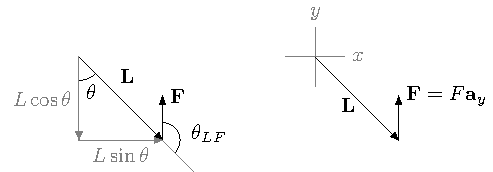
\includegraphics[height=2.5cm]{figBasicFactsVectorCrossProduct}
\begin{tikzpicture}
\coordinate (O) at (4,0,0);
%\coordinate (c) at  ($(a) ! 0.25 ! (b)$);
%\coordinate (d) at  (c)--+($(c)-(O)$);
 %
%axis
\draw[gray](3.5,0)--(4.5,0)node[right]{$x$};
\draw[gray](4,-0.5)--(4,0.5)node[above]{$y$};
%force and moment arm
\draw[-latex] (O)--++(-45:2) node[pos=0.4, below] {${\bf{L}}$};
%\draw[gray] (O)++(-45:2)--++(-45:0.3);
\draw[-latex] (O)++(-45:2)--++(90:0.75) node[right]{${\bf{F}}=F{\bf{a}}_y$};
%\draw (O)++(-45:2)++(0,-0.3) node[below left] {الف};
%\draw (O)++(0,0.1) node[above] {محور};
%
\coordinate (O) at (0,0,0);
%\coordinate (c) at  ($(a) ! 0.25 ! (b)$);
%\coordinate (d) at  (c)--+($(c)-(O)$);
 %
 \pgfmathsetmacro{\SinValue}{2*sin(45)}
\pgfmathsetmacro{\CosValue}{-2*cos(45)}
%
\draw[-latex] (O)--++(-45:2) node[pos=0.4, above right] {${\bf{L}}$};
\draw[gray] (O)++(-45:2)--++(-45:0.75);                       %extending moment arm vector
\draw[-latex] (O)++(-45:2)--++(90:0.75) node[right]{${\bf{F}}$};
%
\draw[gray,-latex] (O)--++(0,\CosValue) node[pos=0.5, left]{$L \cos \theta$};             %moment arm components
\draw[gray,-latex] (O)++(0,\CosValue)--++(\SinValue,0)node[pos=0.5, below]{$L \sin \theta$};
%
\draw[domain=-90:-45] plot ({0.4*cos(\x) },{0.4*sin(\x)});
\node at (0.2,-0.6) {$\theta$};
%
\coordinate (c1) at (-45:2);
%($(<center>) + (<init angle>:<radius>)$) arc (start angle:end angle:radius);
\draw[]  ($(c1) + (-45:0.3)$) arc (-45:90:0.3);
\node at (2.2,-1.3) {$\theta_{LF}$};
\end{tikzpicture}
\caption{کارتیسی نظام میں قوت مروڑ کا حل}
\label{شکل_حقائق_کارتیسی_مروڑ_کا_حل}
\end{figure}
%
\جزوحصہ{نقطی ضرب}
دو سمتی متغیرات  کا ایسا حاصل ضرب جو غیر سمتی متغیر ہو \اصطلاح{نقطی ضرب}\فرہنگ{ضرب!نقطہ}\حاشیہب{dot product}\فرہنگ{dot product} کہلاتا ہے جو درج ذیل لکھا جاتا ہے۔
\begin{align}
\kvec{C}=\kvec{A} \cdot \kvec{B}
\end{align}
نقطی ضرب میں ضرب کے نشان کو نقطہ کی علامت سے ظاہر کیا جاتا ہے جس کی بنا پر اس کا نام نقطی ضرب ہے۔

نقطی ضرب کی مقدار  درج ذیل ہو گی
\begin{gather}
\begin{aligned}\label{مساوات_بنیادی_ضرب_نقطہ_تعریف}
\kvec{C}&=\kvec{A} \cdot \kvec{B}\\
&=\abs{\kvec{A}} \abs{\kvec{B}} \cos \theta_{AB}\\
&=A B \cos \theta_{AB}
\end{aligned}
\end{gather}
جہاں \عددیء{\theta_{AB}} ان سمتیات کے بیچ زاویہ ہے۔

\ابتدا{مثال}
مندرجہ ذیل نقطی ضرب حاصل کریں۔
\begin{itemize}
\item
$\ax \cdot \ax \quad \ay \cdot \ay \quad \az \cdot \az$
\item
$\ax \cdot \ay \quad \ay \cdot \az \quad \arho \cdot \arho \quad \arho \cdot \atheta$
\end{itemize}

حل:اس مثال میں سب سمتیات اکائی  ہیں۔اکائی سمتیہ کا طول ایک (1) کے برابر ہوتا ہے:
\begin{itemize}
\item
$\ax \cdot \ax =(1) (1) \cos 0=1$
\item
$\ay \cdot \ay =(1) (1) \cos 0=1$
\item
$\az \cdot \az =(1) (1) \cos 0=1$
\item
$\ax \cdot \ay =(1) (1) \cos 90\degree=0$
\item
$\ay \cdot \az =(1) (1) \cos 90\degree=0$
\item
$\arho \cdot \arho =(1) (1) \cos 0=1$
\item
$\arho \cdot \atheta =(1) (1) \cos 90\degree=0$
\end{itemize}
\انتہا{مثال}
%=========================
\ابتدا{مثال}
شکل \حوالہ{شکل_حقائق_کارتیسی_کام}  میں قوت \سمتیہ{F} ایک بوجھ کو دھکیل رہی ہے۔سمتی فاصلہ  \سمتیہ{L} طے کرنے پر قوت کتنا کام کر چکی ہو گی۔

حل: کام  \عددیء{W} کی تعریف درج ذیل  ہے۔
\begin{align}
W=\kvec{F} \cdot \kvec{L}
\end{align}
کارتیسی نظام میں سمتی فاصلہ 
\begin{align}
\kvec{L}=L \cos \theta \ax +L \sin \theta \ay
\end{align}
ہو گا۔ یوں درج ذیل ہو گا
\begin{gather}
\begin{aligned}
W &= (F \ax) \cdot (L \cos \theta \ax +L \sin \theta \ay)\\
&=F L \cos \theta (\ax \cdot \ax)+ F L \sin \theta (\ax \cdot \ay)\\
&= F L \cos \theta
\end{aligned}
\end{gather}
%
\begin{figure}
\centering
%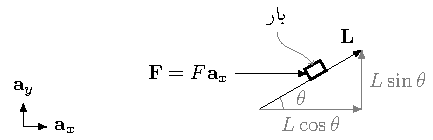
\includegraphics[height=2.5cm]{figBasicFactsWorkAsDotProduct}
\begin{tikzpicture}
%\draw[step=1,gray,thick] (0,0) grid (2,2);
%\draw[step=0.1,gray,thin] (0,0) grid (2,2);
\coordinate (O) at (0,0);
\def\radius{2};
\def\angle{30};
%\coordinate (c) at  ($(a) ! 0.25 ! (b)$);
%\coordinate (d) at  (c)--+($(c)-(O)$);
 %
\pgfmathsetmacro{\SinValue}{\radius*sin(\angle)}
\pgfmathsetmacro{\CosValue}{\radius*cos(\angle)}

\draw[-latex] (O)--(\angle:\radius) node[above left]{{\bf{L}}};
\draw[gray,-latex] (O)--(0:\CosValue) node[pos=0.5,below]{$L \cos \theta$};
\draw[gray,-latex] (O)++(0:\CosValue)--++(90:\SinValue) node[pos=0.5,right]{$L \sin \theta$};

\draw[thick] (O)++(\angle:\radius/2)--++(\angle:0.3)--++(\angle+90:0.2)--++(\angle+90+90:0.3)--cycle;
%\coordinate (p) at ${(O)++(\angle:\radius/2)}!0.5!{}
%($(<center>) + (<init angle>:<radius>)$) arc (start angle:end angle:radius);
\draw[gray]  ($(O) + (0:0.4)$) arc (0:30:0.4);
\node[gray] at (0.7,0.2) {$\theta$};
%force
\draw[latex-](0.8,0.6)--(-0.4,0.6)node[left]{${\bf{F}}=F {\bf{a}}_x$};
%load
\node[above] at (0.3,1.3) {بار};
\draw[thin,gray,->] (0.3,1.3) to [out=-90,in=120] (0.9,0.75);
%unit vectors
\coordinate(UV) at (-4,-0.3);
\draw[-latex] (UV)--++(0.4,0) node[right]{${\bf{a}}_x$};
\draw[-latex] (UV)--++(0,0.4)node[above]{${\bf{a}}_y$};
 %--------------------------------------------
 %\pgfmathsetmacro{\SinValue}{2*sin(45)}
%\pgfmathsetmacro{\CosValue}{-2*cos(45)}
%
%\draw[gray,-latex] (O)--++(0,\CosValue) node[pos=0.5, left]{$L \cos \theta$};             %moment arm components
%\draw[gray,-latex] (O)++(0,\CosValue)--++(\SinValue,0)node[pos=0.5, below]{$L \sin \theta$};
%
%\draw[domain=-90:-45] plot ({0.4*cos(\x) },{0.4*sin(\x)});
%\node at (0.2,-0.6) {$\theta$};
%
%\coordinate (c1) at (-45:2);
%($(<center>) + (<init angle>:<radius>)$) arc (start angle:end angle:radius);
%\draw[]  ($(c1) + (-45:0.3)$) arc (-45:90:0.3);
%\node at (2.2,-1.3) {$\theta_{LF}$};
\end{tikzpicture}
\caption{کارتیسی نظام میں کام}
\label{شکل_حقائق_کارتیسی_کام}
\end{figure}
جہاں پچھلی مثال کی مدد سے \عددیء{\ax \cdot \ax=1} اور \عددیء{\ax \cdot \ay=0} لیے گئے ہیں۔ یہی جواب نقطی ضرب کی تعریف، مساوات \حوالہ{مساوات_بنیادی_ضرب_نقطہ_تعریف}،  سے با آسانی حاصل ہوتا ہے۔
\انتہا{مثال}
%
\حصہ{تفرق  اور جزوی تفرق}
مساوات \حوالہ{مساوات_بنیادی_تفرق} میں ایک تفاعل  کا \اصطلاح{تفرق}\فرہنگ{تفرق}\حاشیہب{differentiation}\فرہنگ{differentiation} دیا گیا ہے، جس میں \عددیء{B_0} ایک مستقل ہے، جبکہ مساوات \حوالہ{مساوات_بنیادی_جزوی_تفرق}  میں ایک تفاعل کا \اصطلاح{جزوی تفرق}\فرہنگ{تفرق!جزوی}\حاشیہب{partial differentiation}  دیا گیا ہے۔
\begin{gather}
\begin{aligned}\label{مساوات_بنیادی_تفرق}
B (\theta )&=B_0 \cos \theta\\
\frac{\dif B}{\dif \theta}&=-B_0 \sin \theta
\end{aligned}
\end{gather} 
%
\begin{align}\label{مساوات_بنیادی_جزوی_تفرق}
\partial W(x,\lambda)=\frac{\partial W}{\partial x} \dif x+\frac{\partial W}{\partial \lambda} \dif \lambda
\end{align}


\حصہ{خطی تکمل}
مساوات \حوالہ{مساوات_بنیادی_سائن_نما_تفاعل}  میں ایک تفاعل \عددیء{B(\theta)} دیا گیا ہے جسے شکل \حوالہ{شکل_حقائق_کوسائن_موج}  میں دکھایا گیا ہے۔ اس کا \اصطلاح{طولِ موج}\فرہنگ{طول موج}\حاشیہب{wavelength}  \عددیء{2 \pi} ریڈیئن ہے۔
\begin{align}\label{مساوات_بنیادی_سائن_نما_تفاعل}
B(\theta)=B_0 \cos \theta
\end{align}
 ہم \عددیء{-\pi/2<\theta<\pi/2} پر اس تفاعل کی اوسط قیمت تلاش کرتے ہیں۔
\begin{align}
B_{\textup{اوسط}}=\frac{B_0}{\pi}\int_{-\frac{\pi}{2}}^{\frac{\pi}{2}} \cos \theta \dif \theta=\frac{2 B_0}{\pi}
\end{align}
اسی طرح ہم \عددیء{-\pi/2<\theta<\pi/2} پر  تفاعل کے مربع، \عددیء{B^2}، کی اوسط تلاش کرتے ہیں۔
\begin{gather}
\begin{aligned}\label{مساوات_بنیادی_سائن_نما_اوسط_مربع}
B^2_{\textup{اوسط}}&=\frac{B_0^2}{\pi}\int_{-\frac{\pi}{2}}^{\frac{\pi}{2}} \cos^2 \theta \dif \theta\\
&=\frac{B_0^2}{\pi}\int_{-\frac{\pi}{2}}^{\frac{\pi}{2}}\frac{1+\cos 2 \theta}{2} \dif \theta\\
&=\frac{B_0^2}{2}
\end{aligned}
\end{gather}
تفاعل کے مربع کی اوسط کا جذر نہایت اہم قیمت ہے جو تفاعل کی \اصطلاح{موثر}\فرہنگ{موثر}\حاشیہب{rms, root mean square}\فرہنگ{rms} قیمت کہلاتی ہے اور  جسے  \عددیء{B_{\textup{موثر}}} لکھا جاتا ہے۔
\begin{align}\label{مساوات_بنیادی_سائن_نما_کی_موثر_قیمت}
B_{\textup{موثر}}=\sqrt{B^2_{\textup{اوسط}}}=\frac{B_0}{\sqrt{2}}
\end{align}
یہ ایک بہت اہم نتیجہ ہے جو آپ کو زبانی یاد ہونا چاہئے۔ یہ مساوات ہر سائن نما تفاعل کے لئے درست ہے۔کسی بھی متغیرہ کے مربع کی اوسط کا جذر اس متغیرہ کی \اصطلاح{موثر}\حاشیہب{effective} قیمت کہلاتی ہے۔
%
\begin{figure}
\centering
%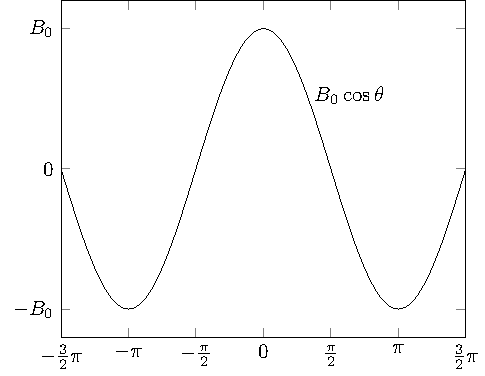
\includegraphics{figBasicFactsCosineWave}
\begin{tikzpicture}
 \begin{axis}[small,enlargelimits=true, xlabel={$\theta$},xlabel style={anchor=west},axis lines=middle, axis line style={-},
     xtick={-6.28,-4.71,-3.14,-1.57,0,1.57,3.14,4.71,6.28},
     xticklabels={$-2\pi$,$-\frac{3}{2}\pi$,$-\pi$,$-\frac{\pi}{2}$,$0$, $\frac{\pi}{2}$,$\pi$,$\frac{3}{2}\pi$,$2\pi$},
  ytick={-1,0,1},
     yticklabels={$-B_0$,$0$,$B_0$}
     ]
      \addplot[domain=-3/2*pi:3/2*pi,samples=200,black]{cos(deg(x))}node[right,pos=0.6]{$B_0 \cos \theta $};
    \end{axis}
\end{tikzpicture}
\caption{کوسائن موج}
\label{شکل_حقائق_کوسائن_موج}
\end{figure}
\حصہ{سطحی تکمل}
فرض کریں   شکل  \حوالہ{شکل_حقائق_نلکی_سطحی_تکمل} میں نلکی کے بیرونی سطح پر سطحی کثافت، \عددیء{B}،  کی قیمت مساوات \حوالہ{مساوات_بنیادی_سائن_نما_تفاعل} دیتی ہے۔  ہم آدھے بیرونی سطح، زاویہ \عددیء{-\pi/2} تا \عددیء{\pi/2}،  کے بیچ اس کی کل مقدار \عددیء{\phi} معلوم کرتے ہیں۔اس سطح میں نلکی کے سر شامل نہیں ہیں۔

ہم نلکی کے بیرونی سطح پر  خطہ \عددیء{abcd} لیتے ہیں جس کی چوڑائی \عددیء{\rho \Delta\theta}، لمبائی \عددیء{l} اور  رقبہ   \عددیء{\Delta A}  ہے۔\عددیء{\Delta \theta} کو نہایت کم کرتے ہوئے  رقبہ \عددیء{\dif A=\rho l \dif \theta} حاصل ہو گا۔اس سطح پر \عددیء{B} کی مقدار محوری لمبائی  کے ساتھ تبدیل نہیں ہوتی ہے۔سطح \عددیء{\dif A}  پر \عددیء{\dif \phi=B \dif A} اور کل \عددیء{\phi} درج ذیل ہو گا۔
\begin{figure}
\centering
%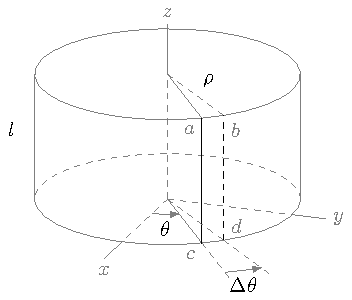
\includegraphics{figBasicFactsCylindricalSurfaceIntegral}
\tdplotsetmaincoords{70}{110}
\begin{tikzpicture}[scale=3,tdplot_main_coords]

%CIRCLE
\coordinate (O) at (0,0,0);
\def\angleA{35};
\def\angleB{45};
\def\kradius{0.75};
\def\height{0.75};

%vectors
%\tdplotsinandcos{\sintheta}{\costheta}{\angleA}%
%\draw[thick,-latex] (0,0,0)--(\kradius * \costheta,\kradius * \sintheta,0);
%\tdplotsinandcos{\sintheta}{\costheta}{\angleB}%
%\draw[gray,-latex] (0,0,0)--(\kradius * \costheta,\kradius * \sintheta,0)  node[pos=0.5, above]{${\rho_0}$};
%text
%\tdplotdrawarc[gray,->]{(0,0,0)}{0.35}{0}{\angleA}{anchor=north,color=black}{$\theta$};

%CYLINDER
%axis for cylinder
\coordinate (O) at (0,0,0);
\coordinate (Otop) at (0,0,\height);

\draw[gray,dashed] (O) -- ++(\kradius,0,0);  %hidden axis
\draw[gray,dashed] (O) -- ++(0,\kradius,0);
\draw[gray,dashed] (O) -- ++(0,0,\height);

\draw[gray] (O)++(\kradius,0,0) -- ++(0.3,0,0)node[below ] {$x$};  %visible axis
\draw[gray] (O)++(0,\kradius,0) -- ++(0,0.2,0)node[right ] {$y$};
\draw[gray] (O)++(0,0,\height) -- ++(0,0,0.3)node[above] {$z$};

%top and bottom of cylinder
\tdplotdrawarc[gray, dashed]{(O)}{\kradius}{110}{290}{}{};   %bottom of cylinder
\tdplotdrawarc[gray]{(O)}{\kradius}{-70}{110}{}{};
\tdplotdrawarc[gray]{(Otop)}{\kradius}{0}{360}{}{};   %top of cylinder
%left edge of cylinder
\tdplotsinandcos{\sintheta}{\costheta}{-70}%
\coordinate (leftLower) at (\kradius * \costheta,\kradius * \sintheta, 0);
\coordinate (leftUpper) at (\kradius * \costheta,\kradius * \sintheta, \height);
\draw[gray](leftLower)--(leftUpper);
%radial solid line
\tdplotsinandcos{\sinthetaA}{\costhetaA}{\angleA}%
\draw[gray] (O)--++(\kradius * \costhetaA,\kradius * \sinthetaA,0)node[below left]{$c$};   %lower radial section
\draw[gray] (Otop)--++(\kradius * \costhetaA,\kradius * \sinthetaA,0)node[below left]{$a$};  %upper radial section
\draw[black](\kradius * \costhetaA,\kradius * \sinthetaA,0)--(\kradius * \costhetaA,\kradius * \sinthetaA,\height);     %vertical section
\draw[gray,dashed] (O)++(\kradius * \costhetaA,\kradius * \sinthetaA,0)--++(0.8*\kradius * \costhetaA,0.8*\kradius * \sinthetaA,0);   %lower radial extension
%radial dashed line
\tdplotsinandcos{\sinthetaB}{\costhetaB}{\angleB}%
\draw[gray,dashed] (O)--++(\kradius * \costhetaB,\kradius * \sinthetaB,0)node[above right]{$d$}; ; %lower radial section
\draw[gray,dashed] (Otop)--++(\kradius * \costhetaB,\kradius * \sinthetaB,0) node[pos=0.5,above right,black]{$\rho$} node[below right,gray]{$b$}; %upper radial section
\draw[black,dashed](\kradius * \costhetaB,\kradius * \sinthetaB,0)--(\kradius * \costhetaB,\kradius * \sinthetaB,\height);    %vertical section
\draw[gray,dashed] (O)++(\kradius * \costhetaB,\kradius * \sinthetaB,0)--++(0.8*\kradius * \costhetaB,0.8*\kradius * \sinthetaB,0);   %lower radial extension
%height is l
\coordinate (leftLowerL) at (0,-1, 0);
\coordinate (leftUpperL) at (0,-1, \height);
\path (leftLowerL)--(leftUpperL) node[pos=0.4,right]{$l$};

%right edge of cylinder
\tdplotsinandcos{\sintheta}{\costheta}{110}%
\coordinate (rightLower) at (\kradius * \costheta,\kradius * \sintheta, 0);
\coordinate (rightUpper) at (\kradius * \costheta,\kradius * \sintheta, \height);
\draw[gray](rightLower)--(rightUpper);
%angles
\tdplotdrawarc[color=gray,-latex,tdplot_main_coords]{(O)}{0.25}{0}{35}{anchor=north,black}{$\theta$};
\tdplotdrawarc[color=gray,-latex,tdplot_main_coords]{(O)}{1.25}{35}{45}{anchor=north,black}{$\Delta \theta$};
\end{tikzpicture}
\caption{نلکی کی بیرونی سطح پر متغیرہ کا تکمل کل مقدار دے گی۔}
\label{شکل_حقائق_نلکی_سطحی_تکمل}
\end{figure}
%
\begin{gather}
\begin{aligned}\label{مساوات_بنیادی_بہاو_بذریع_تکمل_زاویہ_صفر}
\phi&=\int_{-\pi/2}^{\pi/2}\dif \phi=\int_{-\pi/2}^{\pi/2} (B_0 \cos\theta)( \rho l\dif\theta)\\
&=B_0 l \rho \int_{-\pi/2}^{\pi/2} \cos \theta \dif \theta =2 B_0 l \rho
\end{aligned}
\end{gather}
 مساوات \حوالہ{مساوات_بنیادی_بہاو_بذریع_تکمل_زاویہ_صفر}  میں نچلا حد \عددیء{(-\pi/2-\alpha)} اور بالائی کا حد \عددیء{(\pi/2-\alpha)} لینے سے درج ذیل حاصل ہو گا۔
\begin{align}\label{مساوات_بنیادی_بہاو_بذریع_تکمل_کوئی_زاویہ}
\phi (\alpha) = B_0 l \rho \int_{-\frac{\pi}{2}-\alpha}^{\frac{\pi}{2}-\alpha} \cos \theta \dif \theta =2 B_0 l \rho \cos \alpha
\end{align}
نلکی کے بیرونی نصف سطح  پر \عددی{\phi(\alpha)} کی عمومی قیمت  مساوات \حوالہ{مساوات_بنیادی_بہاو_بذریع_تکمل_کوئی_زاویہ} دیتی جو  \عددیء{\alpha} پر منحصر ہے۔ یہ ایک بہت اہم مساوات ہے۔ مساوات \حوالہ{مساوات_بنیادی_بہاو_بذریع_تکمل_کوئی_زاویہ} میں  \عددیء{\alpha=0} پر کرنے سے  مساوات \حوالہ{مساوات_بنیادی_بہاو_بذریع_تکمل_زاویہ_صفر}   حاصل ہوتا ہے۔

\حصہ{ مرحلی سمتیہ}
\begin{figure}
\centering
%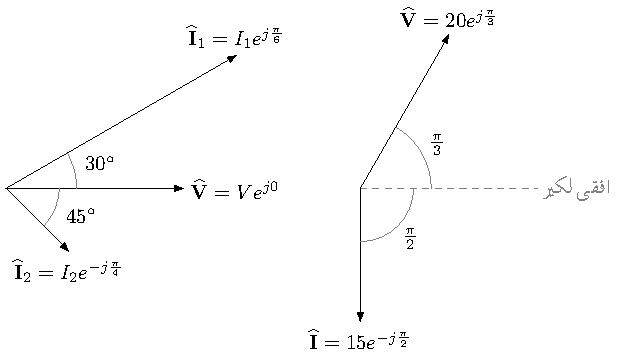
\includegraphics{figBasicFactsPhasors}
\begin{tikzpicture}[scale=3]
\coordinate (Oa) at (0,0);
%phasors
\draw[-latex] (Oa)--++(0:1) node[right]{${\bf{\hat{V}}}=V e^{j 0}$};
\draw[-latex] (Oa)--++(30:1.5) node[above]{${\bf{\hat{I}}}_1=I_1 e^{j \frac{\pi}{6}}$};
\draw[-latex] (Oa)--++(-45:0.5) node[below]{${\bf{\hat{I}}}_2=I_2 e^{-j \frac{\pi}{4}}$};
%
\draw[gray]
  % radius=0.3, initial=0, final=30
  %([shift={(0:0.3)}]c1) arc (0:90:0.3)
  ($(0,0) + (0:0.4)$) arc (0:30:0.4) node[black] at (15:0.55) {$30^\circ$};
\draw[gray]
  % radius=0.3, initial=0, final=90
  %([shift={(0:3mm)}]c1) arc (0:90:3mm)
  ($(0,0) + (0:0.3)$) arc (0:-45:0.3) node[black] at (-20:0.45){$45^\circ$};
%-------
\coordinate (Ob) at (2,0);
%phasors
\draw[gray,dashed] (Ob)--++(0:1) node [right] {لکیر افقی};
\draw[-latex] (Ob)--++(60:1) node[above]{${\bf{\hat{V}}}=20 e^{j \frac{\pi}{3}}$};
\draw[-latex] (Ob)--++(-90:0.75) node[below]{${\bf{\hat{I}}}=15 e^{-j \frac{\pi}{2}}$};
%angles
\draw[gray]
  % radius=0.3, initial=0, final=30
  %([shift={(0:0.3)}]c1) arc (0:90:0.3)
  ($(Ob) + (0:0.4)$) arc (0:60:0.4);
\draw  (Ob)++(30:0.5)node {$\frac{\pi}{3}$};
\draw[gray]
  % radius=0.3, initial=0, final=90
  %([shift={(0:3mm)}]c1) arc (0:90:3mm)
  ($(Ob) + (0:0.3)$) arc (0:-90:0.3);
\draw  (Ob)++(-45:0.4)node {$\frac{\pi}{2}$};
\end{tikzpicture}
\caption{مرحلی سمتیہ}
\label{شکل_حقائق_دوری_سمتیات}
\end{figure}
سائن نما امواج جن کی تعدد معین ہو کو مرحلی سمتیہ سے ظاہر کرنا  مفید ثابت ہوتا ہے۔ مساوات \اصطلاح{یولر}\فرہنگ{یولر مساوات}\حاشیہب{Euler's equation}\فرہنگ{Euler}
\begin{align}
A_0 e^{\mp j (\omega t + \phi)}=A_0 \cos (\omega t +\phi) \mp j \sin (\omega t+\phi)
\end{align}
کی مدد سے کوسائن موج درج ذیل  لکھی جا سکتی ہے۔
\begin{align}
A_0 \cos (\omega t +\phi)=\frac{A_0}{2} \left(e^{j(\omega t +\phi)} -e^{-j(\omega t +\phi)}\right)
\end{align}
اس سے ثابت ہوتا ہے کہ کوسائن موج دراصل دو مخلوط اعداد کا مجموعہ ہے۔ مساوات یولر ایک مخلوط عدد کو ظاہر کرتا ہے جس کے دو جزو ہیں۔ اس کا ایک جزو حقیقی عدد ہے اور اس کا دوسرا جزو فرضی عدد ہے۔اس کا حقیقی جزو کوسائن موج کو ظاہر کرتا ہے۔ لہٰذا ایک کوسائن موج  \عددیء{A_0 e^{j(\omega t +\phi)}} یا \عددیء{A_0 e^{-j(\omega t +\phi)}} کا حقیقی جزو ہوتا ہے۔ رسمی طور پر سائن نما امواج کو \عددیء{A_0 e^{j(\omega t +\phi)}} سے ظاہر کیا جاتا ہے جس کو مختصراً \عددیء{A_0 e^{j\phi}} یا  \عددیء{A_0 \phase{\phi}} لکھا جاتا ہے جو  \اصطلاح{مرحلی سمتیہ}\فرہنگ{مرحلی سمتیہ}\حاشیہب{phasor}\فرہنگ{phasor} کہلاتا ہے۔ مرحلی سمتیہ کا طول \عددیء{A_0} اور افقی لکیر کے ساتھ زاویہ \عددیء{\phi} ہے۔

مرحلی سمتیہ استعمال کرتے وقت آپ کو یہ ذہن میں رکھنا ہو گا کہ یہ درحقیقت ایک کوسائن موج ہے جس کا حیطہ  \عددیء{A_0} ، دوری زاویہ \عددیء{\phi} اور زاویائی تعدد \عددیء{\omega} ہے۔

اس کتاب میں مرحلی سمتیات کو سادہ طرز لکھائی میں انگریزی کے بڑے حروف جن پر ٹوپی کا نشان ہو سے ظاہر کیا جائے گا، یعنی \عددیء{\hat{I},\hat{V}}  وغیرہ اور ان کے طول کو بغیر ٹوپی کے نشان کے اسی حرف سے ظاہر کیا جائے گا۔یوں برقی دباو \عددیء{v= 20 \cos (\omega t +\frac{\pi}{3})} کے لئے درج ذیل درست ہو گا۔
\begin{gather}
\begin{aligned}
v&=20 \cos \big(\omega t +\frac{\pi}{3}\big)\\
\hat{V}&=20 e^{j \frac{\pi}{3}}\\
\hat{V}&=20 \phase{\frac{\pi}{3}}\\
V&=20
\end{aligned}
\end{gather}
اس مساوات میں پہلا جزو ایک عام کوسائن موج ہے جس کو دوسرے جزو میں مرحلی سمتیہ کی صورت میں لکھا گیا ہے۔ تیسرا اس مرحلی سمتیہ کا طول اور چوتھا اس کا زاویہ بتلا رہا ہے۔

مرحلی سمتیات کو عام سمتیات کی طرح ہی تصور کیا جاتا ہے۔ اس مساوات میں \عددیء{\hat{V}} کا طول \عددیء{20} اور افقی لکیر سے زاویہ  \عددیء{\tfrac{\pi}{3}} ریڈیئن ہے۔زاویہ  کو افقی لکیر سے گھڑی کے مخالف رخ ناپا جاتا ہے۔افقی لکیر سے گھڑی کے رخ  منفی زاویہ ہو گا۔ شکل \حوالہ{شکل_حقائق_دوری_سمتیات} میں اس \عددیء{\hat{V}} کے علاوہ چند دوسرے  مرحلی سمتیات بھی  دکھائے گئے ہیں۔

%%%%%%%%%%%%%%%%%%%%%%%%%%%%

برقی ادوار میں عموماً برقی دباو \عددیء{\hat{V}} کی نسبت سے  برقی رو  \عددیء{\hat{I}} کا زاویہ بیان کیا جاتا ہے۔شکل \حوالہ{شکل_حقائق_دوری_سمتیات}   میں \عددیء{\hat{I_1}} تیس درجہ زاویہ برقی دباو سے آگے ہے جبکہ  \عددیء{\hat{I_2}}  پینتالیس درجہ زاویہ برقی دباو کے  پیچھے  ہے۔اس حقیقت کو یوں بیان کیا جاتا ہے کہ \عددیء{\hat{I_1}} تیس درجہ  \اصطلاح{پیش زاویہ}\فرہنگ{پیش زاویہ}\حاشیہب{leading angle}\فرہنگ{leading} پر  ہے جبکہ  \عددیء{\hat{I_2}} پینتالیس درجہ  \اصطلاح{تاخیری زاویہ}\فرہنگ{تاخیری زاویہ}\حاشیہب{lagging angle}\فرہنگ{lagging} پر ہے۔اسے طرح \عددیء{\hat{I_1}} کو \اصطلاح{پیش} برقی رو جبکہ \عددیء{\hat{I_2}} کو \اصطلاح{تاخیری} برقی رو کہا جاتا ہے۔دو مرحلی سمتیات کے آپس میں زاویے کو \اصطلاح{مرحلی فرق}\فرہنگ{مرحلی فرق}\حاشیہب{phase difference}\فرہنگ{phase difference} کہتے ہیں لہٰذا \عددیء{\hat{I_1}} اور \عددیء{\hat{I_2}} میں \عددیء{75 \degree} کا مرحلی فرق پایا جاتا ہے۔یہاں یہ دھیان رہے کہ شکل میں  \عددیء{45\degree} مثبت لکھا گیا ہے۔چونکہ یہ افقی لکیر سے زاویہ ناپنے کی الٹ سمت میں ہے لہٰذا یہ ایک منفی زاویہ ہے۔

اگر \عددیء{v=V_0 \cos \omega t} اور \عددیء{i=I_0 \cos (\omega t +\theta)} ہوں تب برقی طاقت \عددیء{p=V_0 I_0 \cos \theta} کے برابر ہو گا جہاں \عددیء{\cos \theta} کو \اصطلاح{جزو طاقت}\فرہنگ{جزو طاقت}\حاشیہب{power factor}\فرہنگ{power factor}  اور \عددیء{\theta} کو \اصطلاح{زاویہ جزو طاقت}\فرہنگ{زاویہ جزو طاقت}\حاشیہب{power factor angle}\فرہنگ{power factor angle} کہتے ہیں۔ اسی طرح \اصطلاح{تاخیری} زاویہ کی صورت میں \عددیء{\cos \theta} کو \اصطلاح{تاخیری جزو طاقت}\فرہنگ{جزو طاقت!تاخیری}\حاشیہب{lagging power factor}\فرہنگ{power factor!lagging} اور \اصطلاح{پیش} زاویہ کی صورت میں \عددیء{\cos \theta} کو \اصطلاح{پیش جزو طاقت}\فرہنگ{جزو طاقت!پیش}\حاشیہب{leading power factor}\فرہنگ{power factor!leading} کہتے ہیں۔

یہاں مرحلی سمتیوں کو استعمال کر کے ایک سادہ برقی دور حل کرتے ہیں۔ یوں ان سے وابستگی پیدا ہو جائے گی اور ان کا استعمال بھی سیکھ لیں گے۔
\begin{figure}
\centering
%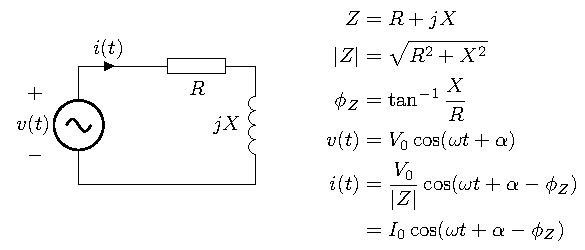
\includegraphics{figBasicFactsRLcircuit}
\begin{tikzpicture}%[circuit ee IEC]
%grid 
%\draw[gray,thick] (0,0) grid (12,3);
%
\draw(0,0)to [short]++(3,0)  to [inductor,l={$jX$}]++(0,2) to [resistor,l_={$R$}]++(-2,0) to [short,i_<=$i(t)$]++ (-1,0) to [sinusoidal voltage source] (0,0); 
\draw node at (-0.8,1){$\begin{aligned} &+ \\  v&(t)\\ &- \end{aligned}$};
%text
\draw node[right] at (4,1){$
\begin{aligned}
Z&=R+j X\\
\left |Z \right|&=\sqrt{R^2+X^2}\\
\phi_Z&=\tan^{-1} \frac{X}{R}\\
v(t)&=V_0 \cos (\omega t +\alpha)\\
i(t)&=\frac{V_0}{\left| Z \right |} \cos (\omega t +\alpha-\phi_Z)\\
&=I_0 \cos (\omega t +\alpha-\phi_Z)
\end{aligned}
$};
\end{tikzpicture}
\caption{مرحلی سمتیہ کی مدد سے \عددیء{RL} دور کا حل۔}
\label{شکل_حقائق_دوری_سمتیہ_سے_دور_حل}
\end{figure}

شکل \حوالہ{شکل_حقائق_دوری_سمتیہ_سے_دور_حل}   ایک سادہ \عددیء{R-L} \اصطلاح{یک مرحلہ}\فرہنگ{یک مرحلہ}\حاشیہب{single phase}\فرہنگ{single phase} برقی دور ہے جس پر لاگو برقی دباو
\begin{gather}
\begin{aligned}
v(t)&=V_0 \cos (\omega t +\alpha)\\
\hat{V}&=V_0 \phase{\alpha}
\end{aligned}
\end{gather}
ہے۔مرحلی سمتیہ کے استعمال سے ہم اس میں برقی رو \عددیء{i(t)} معلوم کرنا چاہتے ہیں۔
\begin{gather}
\begin{aligned}
\hat{I}&=\frac{\hat{V}}{R+j X}=\frac{V_0 \phase{\alpha}}{\abs{Z} \phase {\phi_Z}}\\
&=\frac{V_0}{\abs{Z}} \phase{\alpha-\phi_Z}=I_0 \phase{\alpha-\phi_Z}
\end{aligned}
\end{gather}
جہاں \عددیء{\phi_Z} رکاوٹ کا زاویہ  ہے۔لہٰذا
\begin{align}\label{مساوات_بنیادی_حقائق_دوری_سمتیہ_سے_مزاحمت_امالہ_دور_حل}
i(t)=I_0 \cos (\omega t +\alpha-\phi_Z)
\end{align}
حاصل ہوتا ہے۔یوں \اصطلاح{تاخیری} زاویہ \عددیء{\phi_Z} کے برابر ہے۔

\باب{مقناطیسی ادوار}
%proof read urdu
\حصہ{مزاحمت  اور ہچکچاہٹ}
شکل \حوالہ{شکل_مقناطیسی_دور_مزاحمت_ہچکچاہٹ}  میں ایک سلاخ دکھائی گئی ہے جس کی لمبائی کے رخ   \اصطلاح{مزاحمت}\فرہنگ{مزاحمت}\حاشیہب{resistance}\فرہنگ{resistance}  
\begin{align}\label{مساوات_مقناطیسی_دور_مزاحمت_کی_تعریف}
R=\frac{l }{\sigma A}
\end{align}
ہو گی جہاں  \عددیء{\sigma} \اصطلاح{موصلیت}\فرہنگ{موصلیت}\حاشیہب{conductivity}\فرہنگ{conductivity}  اور \عددیء{A=wh} رقبہ عمودی تراش   ہے۔
\begin{figure}
\centering
\begin{tikzpicture}
\pgfmathsetmacro{\height}{0.75}  
\pgfmathsetmacro{\widthX}{0.25}  
\pgfmathsetmacro{\widthY}{0.25}  
\pgfmathsetmacro{\length}{1.75}  
\coordinate(O) at (0,0,0);
%rod 3d
\draw[black] (O)--(\length,0)node[pos=0.5,below]{$l$}--++(0,\height)--++(-\length,0)--cycle;
\draw[black] (O)++(\length,0)--++(\widthX,\widthY)node[pos=0.4,right]{$w$}--++(0,\height)node[pos=0.5,right]{$h$}--++(-\length,0)--++(-\widthX,-\widthY);
\draw[black] (O)++(\length,0)++(0,\height)--++(\widthX,\widthY);
\draw[gray,-latex] (O)++(0.3*\length,0.5*\height)--++(0.4*\length,0);
\coordinate(textarea) at (\length,2*\height);
\coordinate(flowMid) at (0.5*\length,0.5*\height);
\coordinate(mathEq) at (3*\length,0.7*\height);
\draw[gray,thin,dashed,<-] (flowMid) to [out=90,in=270] (textarea);
%text
\node[anchor = south] at (textarea) {\text{\RL{برقی رو یا مقناطیسی بہاو کا رخ}}};
\node[anchor = east] at (mathEq) {$
\begin{aligned}
R&=\frac{l}{\sigma A}\\
\Re &=\frac{l}{\mu A}
\end{aligned}
$};
\end{tikzpicture}%
\caption{مزاحمت اور ہچکچاہٹ}
\label{شکل_مقناطیسی_دور_مزاحمت_ہچکچاہٹ}
\end{figure}
اس سلاخ کی \اصطلاح{ہچکچاہٹ}\فرہنگ{ہچکچاہٹ}\فرہنگ{reluctance}\حاشیہب{reluctance} \عددیء{\Re}  درج ذیل ہے جہاں \عددیء{\mu}  \اصطلاح{مقناطیسی مستقل}\فرہنگ{مقناطیسی مستقل}\حاشیہب{permeability, magnetic constant}\فرہنگ{permeability}\فرہنگ{magnetic constant} کہلاتا ہے۔ 
\begin{align}\label{مساوات_مقناطیسی_دور_ہچکچاہٹ_کی_تعریف}
\Re = \frac{l}{\mu A}
\end{align}
مقناطیسی مستقل \عددیء{\mu} کو عموماً خلاء کی مقناطیسی مستقل \عددیء{\mu_0=4\pi\, 10^{-7}\,\si{\henry\per\meter}} کی نسبت سے لکھا جاتا ہے یعنی
\begin{align}
\mu=\mu_r \mu_0
\end{align}
جہاں \عددیء{\mu_r} \اصطلاح{جزو مقناطیسی مستقل}\فرہنگ{مقناطیسی مستقل!جزو}\فرہنگ{relative permeability}\فرہنگ{permeability!relative}  کہلاتا ہے۔ہچکچاہٹ کی اکائی \اصطلاح{ایمپیئر-چکر فی ویبر}  ہے جس کی وضاحت جلد کی جائے گی۔
%
\ابتدا{مثال}
شکل \حوالہ{شکل_مقناطیسی_دور_مزاحمت_ہچکچاہٹ}  میں دی گئی سلاخ کی ہچکچاہٹ معلوم کریں جہاں 
\عددیء{\mu_r=2000 }، \عددیء{l=\SI{10}{\centi \meter}}، \عددیء{h=\SI{3}{\centi \meter}} اور \عددیء{w=\SI{2.5}{\centi \meter}} ہیں۔

حل:
\begin{align*}
\Re& = \frac{l}{\mu_r \mu_0 A}\\
&=\frac{10\times 10^{-2}}{2000 \times 4 \pi \times 10^{-7} \times 2.5 \times 10^{-2} \times 3 \times 10^{-2}}\\
&=\SI{53052}{\ampere \cdot turns \per \weber}
\end{align*}
\انتہا{مثال}

\حصہ{کثافتِ برقی رو  اور برقی میدان کی شدت}\شناخت{حصہ_برقی_دور_کثافت_برقی_رو_اور_میدان}
شکل  \حوالہ{شکل_مقناطیسی_دور_کثافت_رو_اور_برقی_شدت} میں ایک موصل سلاخ کے سروں پر برقی دباو \عددی{v}   لاگو کیا گیا ہے۔سلاخ میں  برقی رو \عددیء{i}  \اصطلاح{اوہم} کے قانون\فرہنگ{قانون!اوہم}\حاشیہب{Ohm's law}\فرہنگ{Ohm's law}  سے حاصل ہو گا۔
\begin{align}
i=\frac{v}{R}
\end{align}
درج بالا مساوات کو مساوات \حوالہ{مساوات_مقناطیسی_دور_مزاحمت_کی_تعریف}  کی مدد سے
\begin{align}
i=v \left(\frac{\sigma A}{l}\right)
\end{align}
یعنی
\begin{align}
\frac{i}{A}=\sigma \left(\frac{v}{l} \right)
\end{align}
یا
\begin{align}\label{مساوات_مقناطیسی_دور_اوہم_قانون_کی_تفرق_شکل}
J =\sigma E
\end{align}
لکھا جا سکتا ہے جہاں  \عددی{J} اور \عددی{E} کی تعریفات درج ذیل ہیں۔
\begin{align}
J&=\frac{i}{A} \label{مساوات_مقناطیسی_دور_کثافت_رو}\\
E&=\frac{v}{l} \label{مساوات_مقناطیسی_دور_برقی_شدت}
\end{align}

شکل  \حوالہ{شکل_مقناطیسی_دور_کثافت_رو_اور_برقی_شدت} میں سمتیہ \سمتیہ{J} کی مطلق قیمت \عددیء{J}  اور سمتیہ \سمتیہ{E} کی مطلق قیمت \عددی{E} لیتے ہوئے  مساوات \حوالہ{مساوات_مقناطیسی_دور_اوہم_قانون_کی_تفرق_شکل} کو درج ذیل لکھا جا سکتا ہے
\begin{align}
\kvec{J}=\sigma \kvec{E}
\end{align}
جو قانون اوہم کی دوسری روپ ہے۔ \سمتیہ{J} اور \سمتیہ{E} دونوں کا رخ  \عددیء{\ay}  ہے۔

%
\begin{figure}
\centering
\begin{tikzpicture}
 \pgfmathsetmacro{\height}{0.75}  
\pgfmathsetmacro{\widthX}{0.25}  
\pgfmathsetmacro{\widthY}{0.25}  
\pgfmathsetmacro{\length}{1.75}  
%\draw[gray,thick] (0,0) grid (2,2);
%\draw[help lines,xstep=0.1,ystep=0.1] (0,0) grid (2,2);
\coordinate(O) at (0,0,0);

%rod 3d
\draw[black] (O)--(\length,0)node[pos=0.3,below]{$l$}--++(0,\height)--++(-\length,0)--cycle;
\draw[black] (O)++(\length,0)--++(\widthX,\widthY)--++(0,\height)--++(-\length,0)--++(-\widthX,-\widthY);
\draw[black] (O)++(\length,0)++(0,\height)--++(\widthX,\widthY);
%cross section
\draw[gray,dashed](O)++(0.4*\length,0)--++(0,\height)--++(\widthX,\widthY)--++(0,-\height)--cycle;
%current arrow
\draw[gray,-latex] (O)++(0.4*\length,0.5*\height)++(0.5*\widthX,0.5*\widthY)--++(0.3*\length,0) node [below] {$i$};
%circuit
\draw (O)++(0,0.5*\height+0.12)--++(-0.2,0)--++(0,1.75)--++(0.5*\length+0.2,0);  %left section
\draw[thick] (O)++(0,0.5*\height+0.12)++(-0.2,0)++(0,1.75)++(0.5*\length+0.2,0)++(0,0.2)--++(0,-0.4)node[below]{$v$}; 
\draw (O)++(\length,0.5*\height)++(0.5*\widthX,0.5*\widthY)--++(0.2,0)--++(0,1.75)--++(-0.5*\length-0.2,0)++(0,0.1)--++(0,-0.2); %right section

\draw[gray] (0.85,0.155) to [out=-45,in=180] (1.5,-0.5) node[right] {$A$};
%unit vector
\draw[-latex] (O)++(-1.8,0)--++(-1.4142*\widthX,-1.4142*\widthY)node[below]{${\bf{a}}_x$};
\draw[-latex] (O)++(-1.8,0)--++(2*\widthX,0)node[right]{${\bf{a}}_y$};
\draw[-latex] (O)++(-1.8,0)--++(0,2*\widthY)node[above]{${\bf{a}}_z$};
%equations
\draw (O)++(2*\length,-0.6) node [above right]{$
\begin{aligned}
R&=\frac{l}{\sigma A}\\
i&=\frac{v}{R}=v \left( \frac{\sigma A}{l} \right)\\
\frac{i}{A}&=\sigma \frac{v}{l}\\
J&=\sigma E
\end{aligned}
$};
\end{tikzpicture}%
\caption{کثافتِ برقی رو اور برقی دباو کی شدت}
\label{شکل_مقناطیسی_دور_کثافت_رو_اور_برقی_شدت}
\end{figure}
شکل \حوالہ{شکل_مقناطیسی_دور_کثافت_رو_اور_برقی_شدت} سے ظاہر ہے کہ برقی رو \عددیء{i} سلاخ کے رقبہ عمودی تراش \عددیء{A} سے گزرتا ہے لہٰذا مساوات \حوالہ{مساوات_مقناطیسی_دور_کثافت_رو} کے تحت \عددیء{J}، \اصطلاح{کثافتِ برقی رو}\فرہنگ{کثافت!برقی رو}\حاشیہب{current density} ہو گا۔ اسی طرح مساوات \حوالہ{مساوات_مقناطیسی_دور_برقی_شدت}   سے  واضح ہے کہ \عددیء{E} برقی دباو فی اکائی لمبائی کو ظاہر کرتی ہے لہٰذا  \عددیء{E} کو \اصطلاح{برقی میدان کی شدت}\فرہنگ{برقی میدان!شدت}\حاشیہب{electric field intensity} یا (جہاں متن سے مقناطیسی میدان واضح ہو) مختصراً \اصطلاح{میدانی شدت}  کہتے ہیں۔

بالکل اسی طرح کی مساواتیں مقناطیسی متغیرات کے لئے حصہ \حوالہ{حصہ_برقی_دور_کثافت_مقناطیسی_بہاو_اور_میدان}  میں لکھی جائیں گی۔  

\حصہ{برقی ادوار}
برقی دور میں \اصطلاح{برقی دباو}\فرہنگ{برقی دباو}\حاشیہب{electric voltage}  \عددیء{v}\حاشیہد{برقی دباو کی اکائی وولٹ ہے جو اٹلی کے الِسانڈرو وولٹا کے نام ہے جنہوں نے برقی بیٹری ایجاد کی۔}  کی وجہ سے \اصطلاح{برقی رو}\فرہنگ{برقی رو}\حاشیہب{electric current} \عددیء{i} \حاشیہد{برقی رو کی اکائی ایمپیئر ہے جو فرانس کے انڈرِ میرِ ایمپیئر کے نام ہے جن کا برقی و مقناطیسی میدان میں اہم کردار ہے۔} پیدا ہوتا ہے۔ تانبا\فرہنگ{تانبا}\حاشیہب{copper}   کی موصلیت \عددیء{\sigma=\SI{5.9e7}{\siemens \per \meter}} ہے جو بہت بڑی مقدار ہے۔ موصلیت کی اکائی \عددیء{\si{\siemens \per \meter}}  ہے۔ تانبا کی موصلیت کی مقدار بہت بڑی ہونے کی بنا اس سے بنی تار کی مزاحمت\حاشیہد{مزاحمت کی اکائی اوہم ہے جو جرمنی کے جارج سائمن اوہم کے نام ہے جنہوں نے قانونِ اوہم دریافت کیا۔}  \عددیء{R_{\textup{تار}}}  عموماً قابلِ نظرانداز ہو گی۔  تار میں برقی رو \عددیء{i} گزرنے سے تار کے سروں کے بیچ برقی دباو  \عددیء{\Delta v=i R_{\textup{تار}}} پیدا ہو گا جس کو  \عددیء{R_{\textup{تار}}\to 0} کی بنا  نظر انداز کیا جا سکتا ہے۔یوں تانبے کی تار میں برقی دباو کے گھٹاو کو رد کیا جا سکتا ہے یعنی ہم \عددیء{\Delta v \to 0} لے سکتے ہیں۔ 

شکل \حوالہ{شکل_مقناطیسی_دور_سلسہ_وار_مزاحمتی_ادوار}-الف میں ایک ایسا ہی برقی دور دکھایا گیا ہے جس  میں تانبے کی تار کی مزاحمت کو اکٹھے کر کے ایک ہی جگہ  \عددیء{R_{\textup{تار}}} دکھایا گیا ہے۔اس دور کے لئے درج ذیل لکھا جا سکتا ہے۔
\begin{align}
v&=\Delta v+v_L
\end{align}
تار میں برقی گھٹاو \عددیء{\Delta v} نظرانداز کرتے ہوئے
\begin{align}
v&=v_L
\end{align}
حاصل ہوتا ہے۔اس کا مطلب ہوا کہ  تار میں برقی دباو کا گھٹاو قابل نظرانداز ہونے کی صورت میں لاگو برقی دباو جوں کا توں مزاحمت \عددیء{R_L} تک پہنچتا ہے۔برقی ادوار حل کرتے ہوئے یہی حقیقت بروئے کار لاتے ہوئے تار میں برقی دباو کے گھٹاو کو نظرانداز کیا جاتا ہے۔شکل \حوالہ{شکل_مقناطیسی_دور_سلسہ_وار_مزاحمتی_ادوار}-الف میں ایسا کرنے سے  شکل \حوالہ{شکل_مقناطیسی_دور_سلسہ_وار_مزاحمتی_ادوار}-ب حاصل ہوتا ہے۔یہاں یہ سمجھ لینا ضروری ہے کہ برقی تار کو اس غرض سے استعمال کیا جاتا ہے کہ لاگو برقی دباو کو مقام استعمال تک بغیر گھٹائے پہنچایا جائے۔
\begin{figure}
\centering
\begin{subfigure}[b]{0.45\textwidth}
\centering
\begin{tikzpicture}[american voltages]
\draw (0,0)--(1.5*\xx,0) to [european resistor,l={$R_L$},a={$\begin{aligned}&+\\  &v_L\\  &- \end{aligned}$}] ++(0,\xx) to
 [resistor,a={$+\,\Delta v\,-$},l={$R_{\textup{تار}}$}]++(-\xx,0) to [short,i<=$i$]++(-0.5*\xx,0) to [battery,l_={$v$}] (0,0);
\end{tikzpicture}%
\caption{}
\end{subfigure}\hfill
\begin{subfigure}[b]{0.45\textwidth}
\centering
\begin{tikzpicture}[american voltages]
\draw (0,0)--(\xx,0) to [european resistor,l_={$R_L$}] ++(0,\xx) to [short,i<=$i$] ++(-\xx,0) to [battery,l_={$v$}] (0,0); 
%equations
\draw[above,right] (1.5*\xx,\yy/2) node[right]{$
\begin{aligned}
\Delta v&=i R_{\textup{تار}}\\
R_{\textup{تار}}& \to 0\\
\Delta v& \to 0
\end{aligned}
$};
\end{tikzpicture}%
\caption{}
\end{subfigure}%
\caption{برقی ادوار میں برقی تار کی مزاحمت کو نظر انداز کیا جا سکتا ہے۔}
\label{شکل_مقناطیسی_دور_سلسہ_وار_مزاحمتی_ادوار}
\end{figure}%
%---------------------
\begin{figure}
\centering
\begin{subfigure}[b]{0.40\textwidth}
\centering
\begin{tikzpicture}[american voltages]
\draw (0,0)--(1.5*\xx,0) to [european resistor,l_={$R_2$},i<_=$i_2$]++(0,\yy) to [short,i<=$i_t$]++(-1.5*\xx,0) to [battery,l_={$v$}] (0,0); 
\draw (\xx,\yy) to [european resistor,l_={$R_1$},i_=$i_1$ ,*-*]++(0,-\yy);
\end{tikzpicture}%
\caption{}
\end{subfigure}\hfill
\begin{subfigure}[b]{0.50\textwidth}
\centering
\begin{tikzpicture}[american voltages]
\draw (0,0)--(\xx,0) to [european resistor,l_={$R_t$}] ++(0,\yy) to  [short,i<=$i_t$]++(-\xx,0) to [battery,l_={$v$}] (0,0); 
%equations
\draw (1.5*\xx,\yy/2) node[above,right]{$
\begin{aligned}
\frac{1}{R_t}&=\frac{1}{R_1}+\frac{1}{R_2}\\
i_1&=\frac{v}{R_1}\\
i_2&=\frac{v}{R_2}
\end{aligned}
$};
\end{tikzpicture}%
\caption{}
\end{subfigure}%
\caption{کم مزاحمتی راہ میں برقی رو کی مقدار زیادہ ہو گی۔}
\label{شکل_مقناطیسی_دور_متوازی_مزاحمتی_دور}
\end{figure}%
%

شکل \حوالہ{شکل_مقناطیسی_دور_متوازی_مزاحمتی_دور}  میں دوسری مثال دی گئی ہے۔ یہاں ہم دیکھتے ہیں کہ برقی رو اس راہ زیادہ ہو گا جس کی مزاحمت کم ہو۔ یوں  \عددیء{R_1 < R_2} کی صورت میں \عددیء{i_1>i_2} ہو گا۔


\حصہ{مقناطیسی دور حصہ اول}
مقناطیسی ادوار بالکل برقی ادوار کی طرح ہوتے ہیں۔ بس ان میں برقی دباو \عددیء{v} کی جگہ \اصطلاح{مقناطیسی دباو}\فرہنگ{مقناطیسی دباو}\حاشیہب{magnetomotive force, mmf}\فرہنگ{mmf} \عددیء{\tau} ، برقی رو \عددیء{i}  کی جگہ \اصطلاح{مقناطیسی بہاو}\فرہنگ{مقناطیسی بہاو}\حاشیہب{flux}\فرہنگ{flux} \عددیء{\phi}  اور مزاحمت \عددیء{R} کی جگہ  \اصطلاح{ہچکچاہٹ}\فرہنگ{ہچکچاہٹ}\حاشیہب{reluctance}  \عددیء{\Re} پائے جاتے ہیں۔ یوں  بالکل برقی ادوار کی طرح مقناطیسی ادوار بنائے جا سکتے ہیں۔  ایسا ایک مقناطیسی دور شکل \حوالہ{شکل_مقناطیسی__مقناطیسی_سلسلہ_وار_دور}-الف میں دکھایا گیا ہے۔
\begin{figure}
\centering
\begin{subfigure}[b]{0.40\textwidth}
\centering
\begin{tikzpicture}[american voltages]
\draw (0,0)--(1.5*\xx,0) to [european resistor,l_={$\Re_a$}]++(0,\yy) to [european resistor,l={$\Re_c$},a={$+\, \Delta \tau\, -$}]++ (-\xx,0) to [short,i<=$\phi$]++(-0.5*\xx,0) to [battery,l_={$\tau$}] (0,0); 
\end{tikzpicture}%
\caption{}
\end{subfigure}\hfill
\begin{subfigure}[b]{0.50\textwidth}
\centering
\begin{tikzpicture}[american voltages]
\draw (0,0)--(\xx,0) to [european resistor,l_={$\Re_a$}]++(0,\yy) to [short,i<=$\phi$]++(-\xx,0) to [battery,l_={$\tau$}] (0,0); 
%equations
\draw[] (1.5*\xx,\yy/2) node[right]{$
\begin{aligned}
\Delta \tau&=\phi \Re_c\\
\Re_c& \to 0\\
\Delta \tau& \to 0
\end{aligned}
$};
\end{tikzpicture}
\caption{}
\end{subfigure}
\caption{مقناطیسی دور}
\label{شکل_مقناطیسی__مقناطیسی_سلسلہ_وار_دور}
\end{figure}
%
یہاں بھی کوشش یہی ہے کہ  مقناطیسی دباو \عددیء{\tau}  بغیر گھٹائے ہچکچاہٹ \عددیء{\Re_a} تک پہنچایا جائے۔ خلائی درز کی ہچکچاہٹ  \عددیء{\Re_a}   اور مقناطیسی راہ کی ہچکچاہٹ \عددیء{\Re_c}  ہے۔ یوں \عددیء{\Re_c} قابل نظرانداز ہونے کی صورت میں  شکل \حوالہ{شکل_مقناطیسی__مقناطیسی_سلسلہ_وار_دور}-ب حاصل ہو گا جس میں مقناطیسی بہاو \عددیء{\phi}، بالکل اوہم کے قانون کی طرح، درج ذیل مساوات سے حاصل ہو گا۔
\begin{align}\label{مساوات_مقناطیسی_دور_قانون_اوہم}
\tau=\phi \Re_a
\end{align}
جہاں  \عددیء{\Re_c} قابل  نظرانداز ہو وہاں، سلسلہ وار مزاحمتوں کی طرح،  دو سلسلہ وار ہچکچاہٹوں کا مجموعی ہچکچاہٹ  \عددیء{\Re_s}  استعمال کر کے برقی بہاو حاصل ہو گا۔
\begin{align}
\Re_s&=\Re_a+\Re_c\\
\tau&=\phi \Re_s \label{مساوات_مقناطیسی_دور_مقناطیسی_اوہم_قانون}
\end{align}

برقی دور کی طرح، مقناطیسی دباو کو کم ہچکچاہٹ کی راہ استعمال کرتے ہوئے مقام ضرورت تک پہنچایا جاتا ہے۔ مساوات \حوالہ{مساوات_مقناطیسی_دور_ہچکچاہٹ_کی_تعریف}   کے تحت  ہچکچاہٹ کی قیمت  مقناطیسی مستقل \عددیء{\mu} پر منحصر ہے ۔مقناطیسی مستقل کی اکائی   ہینری فی میٹر \عددیء{\si{\henry \per \meter}} ہے۔\عددیء{\mu} کو عموماً \عددیء{\mu=\mu_r \mu_0} لکھا جاتا ہے جہاں  \عددیء{\mu_0=4 \pi \times 10^{-7}} ہینری فی میٹر کے برابر ہے اور \عددیء{\mu_r} کو \اصطلاح{جزو مقناطیسی مستقل}\فرہنگ{مقناطیسی مستقل!جزو}\حاشیہب{relative permeability, relative magnetic constant} کہتے ہیں۔ لوہا،  کچھ دھاتیں اور چند جدید مصنوعی مواد  ایسی ہیں جن کی \عددیء{\mu_r} کی قیمت \عددیء{\num{2000}} اور \عددیء{\num{80000}} کے  بیچ پائی جاتی ہیں۔ مقناطیسی دباو کو  ایک مقام سے دوسری مقام منتقل کرنے کے لئے ان ہی مقناطیسی مواد کو  استعمال کیا جاتا ہے۔

 بد قسمتی سے  مقناطیسی مواد کے  \عددیء{\mu} کی قیمت اتنی زیادہ  نہیں ہوتی ہے کہ ان سے بنی سلاخ کی ہچکچاہٹ ہر موقع پر قابل نظرانداز ہو۔ مساوات \حوالہ{مساوات_مقناطیسی_دور_ہچکچاہٹ_کی_تعریف}  کے تحت  ہچکچاہٹ کم سے کم کرنے کی خاطر رقبہ عمودی تراش کو زیادہ سے زیادہ اور لمبائی کو کم سے کم  کرنا ہو گا۔ یوں مقناطیسی دباو منتقل کرنے کے لئے  باریک تار نہیں بلکہ خاصا زیادہ رقبہ عمودی تراش کا مقناطیسی راستہ  درکار ہوتا ہے۔

مقناطیسی مشین، مثلاً موٹر اور ٹرانسفارمر، کا بیشتر حصہ مقناطیسی دباو منتقل کرنے والے ان مقناطیسی مواد  پر مشتمل ہوتا ہے۔ایسے مشینوں کے قلب میں عموماً یہی مقناطیسی مادہ پایا جاتا ہے لہٰذا ایسا مواد  \اصطلاح{مقناطیسی قالب}\فرہنگ{مقناطیسی قالب}\حاشیہب{magnetic core}\فرہنگ{magnetic core} کہلاتا ہے (شکل \حوالہ{شکل_مقناطیسی__کثافت_مقناطیسی_بہاو_اور_شدت})۔

برقی مشینوں میں مستعمل  مقناطیسی قالب لوہے کی باریک چادر یا پتری\فرہنگ{پتری}\حاشیہب{laminations}\فرہنگ{laminations}  تہہ  در تہہ رکھ کر بنایا جاتا ہے۔ مقناطیسی قالب کے بارے میں مزید معلومات حصہ \حوالہ{حصہ_مقناطیسی_دور_مقناطیسی_مادہ_کے_خصوصیات}  میں  فراہم کی جائے گی۔

\حصہ{کثافتِ مقناطیسی بہاو  اور مقناطیسی میدان کی شدت}\شناخت{حصہ_برقی_دور_کثافت_مقناطیسی_بہاو_اور_میدان}
حصہ \حوالہ{حصہ_برقی_دور_کثافت_برقی_رو_اور_میدان}  میں  برقی دور کی مثال دی گئی۔یہاں شکل \حوالہ{شکل_مقناطیسی__کثافت_مقناطیسی_بہاو_اور_شدت} میں دکھائے گئے مقناطیسی دور پر غور کرتے ہیں۔  مقناطیسی قالب کا \عددیء{\mu_r = \infty} تصور کرتے ہوئے آگے بڑھتے ہیں۔ یوں  قالب کی ہچکچاہٹ \عددیء{\Re_c} صفر ہو گی۔ حصہ \حوالہ{حصہ_برقی_دور_کثافت_برقی_رو_اور_میدان}   میں تانبا کی تار کی طرح یہاں  مقناطیسی قالب کو مقناطیسی دباو \عددیء{\tau} ایک مقام سے دوسری مقام تک منتقل کرنے کے لئے استعمال کیا گیا ہے۔ شکل \حوالہ{شکل_مقناطیسی__کثافت_مقناطیسی_بہاو_اور_شدت} میں مقناطیسی دباو کو خلائی درز کی ہچکچاہٹ \عددیء{\Re_a} تک پہنچایا گیا ہے۔ یہاں \عددیء{\Re_c} کو نظرانداز کرتے ہوئے  کل ہچکچاہٹ کو خلائی درز کی ہچکچاہٹ کے برابر تصور کیا جا سکتا ہے:
\begin{figure}
\centering
\begin{tikzpicture}
\def\height{2};
\def\width{1.5};
\def\thick{0.4};
\def\depthX{0.2};
\def\depthY{0.2};
\def\gap{0.05};
\pgfmathsetmacro{\widthX}{0.25}  
\pgfmathsetmacro{\widthY}{0.25}  
\coordinate(O) at (-0.5,0);
%grid
%\draw[gray,thick](0,0) grid (12,3);
%\draw[gray,thin,xstep=0.1,ystep=0.1](0,0) grid (12,3);
%going clockwise from origin
\draw(0,0)--++(0,\height)--++(\width,0)node[pos=0.5,pin=45:قالب{}]{}--++(0,-0.5*\height+\gap)--++(-\thick,0)--++(0,0.5*\height-\gap-\thick)--++(-\width+2*\thick,0)--++(0,-\height+2*\thick)--++(\width-2*\thick,0)--++(0,0.5*\height-\thick-\gap)--++(\thick,0)--++(0,-0.5*\height+\gap)--cycle;
%
\draw(\thick,\thick)--++(\depthX,\depthY) --++(0,\height-2*\thick-\depthY);
\draw(0.4,0.4)--++(\width-2*\thick-\depthX,0);
\draw(0,\height)--++(\depthX,\depthY)--++(\width,0)--++(-\depthX,-\depthY);
\draw(\width,\height)++(\depthX,\depthY)--++(0,-0.5*\height+\gap)--++(-\depthX,-\depthY);
\draw(\width,0)--++(\depthX,\depthY)--++(0,0.5*\height-\gap)--++(-\depthX,-\depthY);
\draw(\thick+\depthX,\thick+\depthY)--++(\width-2*\thick-\depthX,0);
%gap
\draw(1.7,1.155)--++(-0.1,0);
\draw(1.1,0.95)--++(0.1,0.1);
%winding
\draw (0.6,1.4) to [out=45,in=0] (0.2,1.5) to [short,i_<=$i$] (-1,1.5) node[left]{$+$};
\foreach \l in {1.4,1.2,1}{
\draw (0,\l) to [out=-135,in=45] (0.6,\l-0.2);
}
\draw (0,0.8) to (-1,0.8)node[left]{$-$};
%turns
\node at (0,1.15)[left]{$\tau=N i$};
%gap
\draw[gray](1.8,1.15)--++(0.3,0);
\draw[gray](1.8,1.25)--++(0.3,0);
\draw[->](2.2,1.7)node[right]{$l_a$}--++(-0.2,-0.2)--++(0,-0.25);
\draw[->](2,1)--++(0,0.15);
%flux
\draw[-latex,gray](1.1,1.8)node[left,black]{$\phi$}--++(0.2,0)--++(0,-\height+\thick)--++(-\width+\thick,0)--++(0,\height-\thick)--++(0.5,0);
%urdu coil
\draw[thin,<-](0.3,0.9) to [out=-90,in=60] (-0.7,-0.3)node[below]{\RL{چکر کا لچھا}$\,N$};
%equations
\node at (4,1)[right]{$
\begin{aligned}
H_a&=\frac{\tau}{l_a}\quad \quad B_a&=\frac{\phi_a}{A_a}\\
l_a& \ll w \\
l_a&\ll b 
\end{aligned}
$};
%dimensions
\draw[stealth-stealth] (1.1,-0.1)--++(0.4,0)node[below,pos=0.5]{$b$};
\draw[stealth-stealth](1.5+0.1,-0.1)--++(0.2,0.2)node [pos=0.4,right]{$w$};
%unit vector
\draw[-latex] (O)++(-1.8,0)--++(-1.4142*\widthX,-1.4142*\widthY)node[below]{${\bf{a}}_x$};
\draw[-latex] (O)++(-1.8,0)--++(2*\widthX,0)node[right]{${\bf{a}}_y$};
\draw[-latex] (O)++(-1.8,0)--++(0,2*\widthY)node[above]{${\bf{a}}_z$};
\end{tikzpicture}%
\caption{کثافتِ مقناطیسی بہاو اور مقناطیسی میدان کی شدت۔}
\label{شکل_مقناطیسی__کثافت_مقناطیسی_بہاو_اور_شدت}
\end{figure}
%
\begin{align}
\Re_a=\frac{l_a}{\mu_0 A_a}
\end{align}
خلائی درز کی لمبائی \عددیء{l_a} قالب کے رقبہ عمودی تراش کے اضلاع \عددیء{b} اور \عددیء{w} سے بہت کم ہونے کی صورت ، یعنی  \عددیء{l_a \ll b} اور \عددیء{l_a \ll w}، میں خلائی درز کے رقبہ عمودی تراش \عددیء{A_a} کو قالب کے رقبہ عمودی تراش \عددیء{A_c} کے برابر تصور کیا  جا سکتا ہے:
\begin{align}
A_a=A_c=w b
\end{align}
اس کتاب میں جہاں بتلایا نہ گیا ہو وہاں \عددیء{l_a \ll b} اور \عددیء{l_a \ll w} تصور کرتے ہوئے \عددیء{A_a=A_c} لیا جائے گا۔
 
مقناطیسی دباو \عددی{\tau} کی تعریف درج ذیل مساوات  پیش کرتی ہے۔
\begin{align}
\tau=N i
\end{align}
یوں برقی تار کے چکر ضرب تار میں برقی رو کو مقناطیسی دباو کہتے ہیں۔ مقناطیسی دباو کی اکائی \اصطلاح{ایمپیئر-چکر}\فرہنگ{ایمپیئر-چکر}\حاشیہب{ampere-turn}\فرہنگ{ampere-turn}  ہے۔ حصہ \حوالہ{حصہ_برقی_دور_کثافت_برقی_رو_اور_میدان}   کی طرح ہم مساوات \حوالہ{مساوات_مقناطیسی_دور_مقناطیسی_اوہم_قانون} کو یوں لکھ سکتے ہیں۔
\begin{align}\label{مساوات_مقناطیسی_ڈور_بہاو_مساوی_دباو_بٹا_ہچکچاہٹ}
\phi_a=\frac{\tau}{\Re_a}
\end{align}
مقناطیسی بہاو کی اکائی\فرہنگ{ویبر}\حاشیہب{Weber}\فرہنگ{Weber} \اصطلاح{ویبر}\حاشیہد{یہ اکائی جرمنی کے ولیم اڈورڈ ویبر کے نام ہے جن کا برقی و مقناطیسی میدان میں اہم کردار رہا ہے}  اور ہچکچاہٹ کی اکائی \اصطلاح{ایمپیئر-چکر فی ویبر}\حاشیہب{ampere-turn per weber} ہے۔ اس سلسلہ وار دور کے خلائی درز میں مقناطیسی بہاو \عددیء{\phi_a} اور قالب میں مقناطیسی بہاو \عددیء{\phi_c} ایک دوسرے کے برابر ہوں گے۔درج بالا مساوات کو مساوات \حوالہ{مساوات_مقناطیسی_دور_ہچکچاہٹ_کی_تعریف}   کی مدد سے
\begin{align}
\phi_a &=\tau \left(\frac{\mu_0 A_a}{l_a} \right) \nonumber \\
\intertext{یا}
\frac{\phi_a}{A_a}&=\mu_0 \left( \frac{\tau}{l_a} \right) \label{مساوات_مقناطیسی_دور_کثافت_بہاو_اوہم_قانون_سے}
\end{align}
 لکھ سکتے ہیں جہاں درز کی نشاندہی زیر نوشت میں \عددی{a} لکھ کر کی گئی ہے۔ اس مساوات میں بائیں ہاتھ مقناطیسی بہاو فی اکائی رقبہ کو \اصطلاح{کثافتِ مقناطیسی بہاو}\فرہنگ{مقناطیسی بہاو!کثافت}\حاشیہب{magnetic flux density}\فرہنگ{magnetic flux!density} \عددیء{B_a} اور دائیں ہاتھ مقناطیسی دباو فی اکائی لمبائی کو \اصطلاح{مقناطیسی میدان کی شدت}\فرہنگ{مقناطیسی میدان!شدت}\حاشیہب{magnetic field intensity}\فرہنگ{magnetic field!intensity}  \عددیء{H_a} لکھا جا سکتا ہے:
\begin{align}
B_a&=\frac{\phi_a}{A_a}\\
H_a&=\frac{\tau}{l_a}
\end{align}
کثافتِ مقناطیسی بہاو کی اکائی \اصطلاح{ویبر فی مربع میٹر} ہے جس کو \اصطلاح{ٹسلا}\فرہنگ{ٹسلا}\فرہنگ{Tesla}\حاشیہد{Tesla:  یہ اکائی سربیا کے نِکولا ٹسلا کے نام ہے جنہوں نے بدلتا رو برقی طاقت عام کرنے میں اہم کردار ادا کیا۔}  کا نام دیا گیا ہے۔مقناطیسی میدان کی شدت کی اکائی \اصطلاح{ایمپیئر فی میٹر}\حاشیہب{ampere per meter}  ہے۔ یوں مساوات \حوالہ{مساوات_مقناطیسی_دور_کثافت_بہاو_اوہم_قانون_سے} کو درج ذیل لکھا جا سکتا ہے۔
\begin{align}
B_a=\mu_0 H_a
\end{align}
جہاں متن سے واضح ہو کہ مقناطیسی میدان کی بات ہو رہی ہے وہاں مقناطیسی میدان کی شدت کو مختصراً \اصطلاح{میدانی شدت}\حاشیہب{field intensity} کہا جاتا ہے۔

شکل \حوالہ{شکل_مقناطیسی__کثافت_مقناطیسی_بہاو_اور_شدت} میں خلائی درز میں مقناطیسی بہاو کا رخ  اکائی سمتیہ \عددیء{\az}  کا مخالف ہے لہٰذا کثافتِ مقناطیسی بہاو \عددیء{\kvec{B_a}=-B_a \az} لکھا جا سکتا ہے۔ اسی طرح خلائی درز میں مقناطیسی دباو  اکائی سمتیہ \عددیء{\az} کی مخالف رخ دباو ڈال رہا ہے لہٰذا مقناطیسی دباو کی شدت  \عددیء{\kvec{H_a}=-H_a \az} لکھی جائے گی۔ اس طرح درج بالا مساوات کو درج ذیل سمتی روپ میں  لکھا جا سکتا ہے۔
\begin{align}
\kvec{B_a}=\mu_0 \kvec{H_a}
\end{align}
خلاء کی جگہ کوئی دوسرا مادہ ہونے کی صورت میں یہ مساوات  درج ذیل روپ اختیار کرتی ہے۔
\begin{align}
\kvec{B}=\mu \kvec{H}
\end{align}
%
\ابتدا{مثال}
شکل \حوالہ{شکل_مقناطیسی__کثافت_مقناطیسی_بہاو_اور_شدت} میں خلائی درز میں کثافتِ مقناطیسی بہاو \عددیء{0.1} ٹسلا درکار ہے۔قالب کی \عددیء{\mu_r=\infty}  ہے، خلائی درز کی لمبائی \عددیء{1} ملی میٹر اور  قالب کے گرد برقی تار کے چکر  \عددیء{100} ہیں۔ درکار برقی رو \عددی{i} تلاش کریں۔

حل:\quad
مساوات \حوالہ{مساوات_مقناطیسی_دور_قانون_اوہم} سے 
\begin{align*}
\tau&=\phi \Re\\
N i &= \phi \left(\frac{l}{\mu_0 A} \right)\\
\frac{\phi}{A}&=B=\frac{ N i \mu_0}{l}
\end{align*}
لکھ کر درج ذیل حاصل ہو گا۔
\begin{align*}
0.1&=\frac{100 \times i \times 4 \pi  10^{-7}}{0.001}\\
i&=\frac{0.1 \times 0.001}{100 \times 4 \pi  10^{-7}}=\SI{0.79577}{\ampere}
\end{align*}
\عددیء{i=\SI{0.79577}{\ampere}} برقی رو  خلائی درز میں \عددیء{B=\SI{0.1}{\tesla}} کثافتِ مقناطیسی بہاو پیدا کرے گا۔
\انتہا{مثال}
%
\حصہ{مقناطیسی دور حصہ دوم}
شکل \حوالہ{شکل_مقناطیسی__سادہ_مقناطیسی_دور_بغیر_درز} میں ایک سادہ مقناطیسی نظام دکھایا گیا ہے جس میں قالب کے مقناطیسی مستقل کو محدود تصور کرتے ہیں۔مقناطیسی دباو  \عددیء{\tau=N i} مقناطیسی قالب میں مقناطیسی بہاو \عددیء{\phi_c} پیدا کرتا ہے۔ قالب کا رقبہ عمودی تراش \عددیء{A_c}  ہر مقام پر  یکساں ہے اور قالب  کی اوسط لمبائی \عددیء{l_c} ہے۔ قالب میں مقناطیسی بہاو  کا رخ
  \اصطلاح{فلیمنگ کے دائیں ہاتھ قانون}\حاشیہد{فلیمنگ!دایاں ہاتھ قانون}  سے\حاشیہب{Fleming's right hand rule} معلوم کیا جا سکتا ہے۔اس قانون کو دو طریقوں سے بیان کیا جا سکتا ہے۔
\begin{itemize}
\item
اگر ایک لچھے کو دائیں ہاتھ سے یوں پکڑا  جائے کہ ہاتھ کی چار انگلیاں لچھے میں برقی رو کے رخ لپٹی  ہوں تب انگوٹھا اُس مقناطیسی بہاو کے رخ ہو گا جو اس برقی رو کی وجہ سے وجود میں آیا ہو۔
\item
اگر ایک تار جس میں برقی رو کا گزر ہو کو دائیں ہاتھ سے یوں پکڑا جائے کہ انگوٹھا  برقی رو  کے رخ ہو تب باقی چار انگلیاں اُس مقناطیسی  بہاو کے رخ لپٹی ہوں گی  جو اس برقی رو کی وجہ سے  پیدا ہو گا۔
\end{itemize}

ان دو بیانات میں پہلا بیان  لچھے میں مقناطیسی بہاو کا رخ معلوم کرنے کے لئے زیادہ آسان ثابت ہوتا ہے جبکہ  سیدھی تار کے گرد مقناطیسی بہاو کا رخ دوسرے بیان سے زیادہ آسانی سے معلوم کیا جا سکتا ہے۔
\begin{figure}
\centering
\begin{tikzpicture}
\def\height{2};
\def\width{1.5};
\def\thick{0.4};
\def\depthX{0.2};
\def\depthY{0.2};
\def\gap{0.05};
%grid
%\draw[gray,thick](0,0) grid (5,3);
%\draw[gray,thin,xstep=0.1,ystep=0.1](0,0) grid (5,3);
%going clockwise from origin
\draw(0,0)--++(0,\height)--++(\width,0)--++(0,-\height)--cycle;
\draw(0,0)++(\thick,\thick)--++(0,\height-2*\thick)--++(\width-2*\thick,0)--++(0,-\height+2*\thick)--cycle;
%
\draw(\thick,\thick)--++(\depthX,\depthY) --++(0,\height-2*\thick-\depthY);
\draw(\thick,\thick)--++(\depthX,\depthY) --++(\width-2*\thick-\depthX,0);
\draw(0,\height)--++(\depthX,\depthY)--++(\width,0)--++(-\depthX,-\depthY);
\draw(\width,0)--++(\depthX,\depthY)--++(0,\height)--++(-\depthX,-\depthY);
%flux
\draw[gray,-latex](1.1,1.8)node[left,black]{$\phi_c$}--++(0.2,0)--++(0,-\height+\thick)--++(-\width+\thick,0)--++(0,\height-\thick)--++(0.3,0);
%winding
\draw (0.6,1.4) to [out=45,in=0] (0.2,1.5) to [short,i_<=$i$] (-1,1.5) node[left]{$+$};
\foreach \l in {1.4,1.2,1}{
\draw (0,\l) to [out=-135,in=45] (0.6,\l-0.2);
}
\draw (0,0.8) to (-1,0.8)node[left]{$-$};
%turns
\node at (0,1.15)[left]{$\tau=N i$};
%urdu coil
\draw[thin,<-](0.3,0.9) to [out=-90,in=60] (-0.7,-0.3)node[below]{\RL{چکر کا لچھا}$\,N$};
%dimensions
\draw[stealth-stealth] (1.1,-0.1)--++(0.4,0)node[below,pos=0.5]{$b$};
\draw[stealth-stealth](1.5+0.1,-0.1)--++(0.2,0.2)node [pos=0.4,right]{$w$};
%cross sectional area
\draw[gray](1.1,1)--++(\thick,0)--++(\depthX,\depthY)--++(-\thick,0)--cycle;
\draw[gray,<-] (1.6,1.2) to [out=90,in=-90](2.4,1.7)node[above right,black]{$A_c=b w$};
\draw[gray,<-](1.3,0.6) to [out=0,in=-180] (2.7,1)node [right,black]{\RL{اس لکیر پر اوسط لمبائی $\,l_c\,$ ہے۔}};
\end{tikzpicture}%
\caption{سادہ مقناطیسی دور۔}
\label{شکل_مقناطیسی__سادہ_مقناطیسی_دور_بغیر_درز}
\end{figure}

قالب میں مقناطیسی بہاو  گھڑی وار ہے۔ مقناطیسی بہاو \عددی{\phi} کو  شکل \حوالہ{شکل_مقناطیسی__سادہ_مقناطیسی_دور_بغیر_درز} میں  ہلکی سیاہی کے تیر دار لکیر  سے ظاہر کیا گیا ہے۔ قالب کی ہچکچاہٹ 
\begin{align*}
\Re_c&=\frac{l_c}{\mu_c A_c}
\end{align*}
لکھتے ہوئے مقناطیسی بہاو 
\begin{align*}
\phi_c&=\frac{\tau}{\Re_c}=N i \left(\frac{\mu_c A_c}{l_c} \right)
\end{align*}
ہو گا۔یوں  تمام نا معلوم متغیرات حاصل ہو چکے۔
%
\ابتدا{مثال}
شکل \حوالہ{شکل_مقناطیسی__درز_اور_ہچکچاہٹ}  میں ایک مقناطیسی قالب دکھایا گیا ہے جس کی معلومات درج ذیل ہیں۔
\begin{align}
\text{قالب}= \left\{ 
  \begin{array}{l l}
  h=\SI{20}{\centi\meter} & m=\SI{10}{\centi \meter}\\
 n=\SI{8}{\centi\meter} & w=\SI{2}{\centi \meter}\\
 l_a=\SI{1}{\milli\meter} & \mu_r =\num{40000} \\
 \end{array} \right.
\end{align}
قالب اور خلائی درز کی ہچکچاہٹیں تلاش کریں۔
\begin{figure}
\centering
\begin{tikzpicture}
\def\height{2};
\def\width{1.5};
\def\thick{0.4};
\def\depthX{0.2};
\def\depthY{0.2};
\def\gap{0.05};
%grid
%\draw[gray,thick](0,0) grid (12,3);
%\draw[gray,thin,xstep=0.1,ystep=0.1](0,0) grid (12,3);
%going clockwise from origin
\draw(0,0)--++(0,\height)--++(\width,0)--++(0,-0.5*\height+\gap)--++(-\thick,0)--++(0,0.5*\height-\gap-\thick)--++(-\width+2*\thick,0)--++(0,-\height+2*\thick)--++(\width-2*\thick,0)--++(0,0.5*\height-\thick-\gap)--++(\thick,0)--++(0,-0.5*\height+\gap)--cycle;
%
\draw(\thick,\thick)--++(\depthX,\depthY) --++(0,\height-2*\thick-\depthY);
\draw(0.4,0.4)--++(\width-2*\thick-\depthX,0);
\draw(0,\height)--++(\depthX,\depthY)--++(\width,0)--++(-\depthX,-\depthY);
\draw(\width,\height)++(\depthX,\depthY)--++(0,-0.5*\height+\gap)--++(-\depthX,-\depthY);
\draw(\width,0)--++(\depthX,\depthY)--++(0,0.5*\height-\gap)--++(-\depthX,-\depthY);
\draw(\thick+\depthX,\thick+\depthY)--++(\width-2*\thick-\depthX,0);
%gap
\draw(1.7,1.155)--++(-0.1,0);
\draw(1.1,0.95)--++(0.1,0.1);

%gap
\draw[gray](1.8,1.15)--++(0.3,0);
\draw[gray](1.8,1.25)--++(0.3,0);
\draw[->](2.2,1.7)node[right]{$l_a$}--++(-0.2,-0.2)--++(0,-0.25);
\draw[->](2,1)--++(0,0.15);
%flux
\draw[gray](1.1,1.8)--++(0.2,0)--++(0,-\height+\thick)--++(-\width+\thick,0)--++(0,\height-\thick)--++(0.5,0)--cycle;
%dimensions
\draw[stealth-stealth] (1.1,-0.1)--++(0.4,0)node[below,pos=0.5]{$b$};
\draw[stealth-stealth](1.5+0.1,-0.1)--++(0.2,0.2)node [pos=0.4,right]{$w$};
\draw[stealth-stealth] (-0.1,0)--++(0,\height) node [left,pos=0.5]{$h$};
\draw[stealth-stealth] (-0.3,0)--++(0,0.4) node [left,pos=0.5]{$b$};
\draw (-0.05,0)--++(-0.4,0);
\draw (-0.2,0.4)--++(-0.2,0);
\draw[stealth-stealth](\thick,-0.1)--++(\width-2*\thick,0)node[pos=0.5,below]{$n$};
\draw[stealth-stealth](0,-0.7)--++(\width,0)node[pos=0.5,below]{$m$};
\draw[gray,stealth-](0.8,1.8) to [out=90,in=180] (2,2.7) node[right,black]{$\,l_c\,$ \RL{مرکز کی لمبائی}};
%equations
\draw (4,0) node[above right]{$
\begin{aligned}
A_a&=A_c=bw\\
b&=\frac{m-n}{2}\\
l_c&=2(h-b)+2(m-b)-l_a
\end{aligned}
$};
\end{tikzpicture}%
\caption{خلائی درز اور قالب کے ہچکچاہٹ۔}
\label{شکل_مقناطیسی__درز_اور_ہچکچاہٹ}
\end{figure}

حل:\quad
\begin{align*}
b&=\frac{m-n}{2}=\frac{0.1-0.08}{2}=\SI{0.01}{\meter}\\
A_a&=A_c=bw=0.01 \times 0.02=\SI{0.0002}{\square \meter}\\
l_c&=2(h-b)+2(m-b)-l_a\\
&=2(0.2-0.01)+2(0.1-0.01)-0.001=\SI{0.559}{\meter}
\end{align*}
%
\begin{align*}
\Re_c&=\frac{l_c}{\mu_r \mu_0 A_c}=\frac{0.559}{40000 \times 4 \pi 10^{-7} \times 0.0002}=\SI{55605}{\ampere \cdot t \per \weber}\\
\Re_a&=\frac{l_a}{\mu_0 A_a}=\frac{0.001}{4 \pi 10^{-7} \times 0.0002}=\SI{3978874}{\ampere \cdot t \per \weber}
\end{align*}
قالب کی لمبائی خلائی درز کی لمبائی سے \عددیء{359} گنا زیادہ ہونے کے باوجود خلائی درز کی ہچکچاہٹ قالب کی ہچکچاہٹ سے \عددیء{72} گنا زیادہ ہے۔یوں  \عددیء{\Re_a  \gg \Re_c} ہو گا۔
\انتہا{مثال}
%
\ابتدا{مثال}
شکل  \حوالہ{شکل_مقناطیسی_دور_سادہ_گھومتا_مشین} سے رجوع کریں۔خلائی درز \عددیء{5} ملی میٹر لمبا ہے اور گھومتے حصہ پر \عددیء{1000} چکر ہیں۔خلائی درز میں \عددیء{\SI{0.95}{\tesla}} کثافتِ مقناطیسی بہاو حاصل کرنے کی خاطر درکار برقی رو معلوم کریں۔
\begin{figure}
\centering
%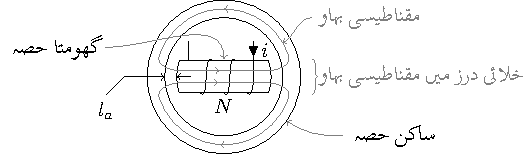
\includegraphics{figMagneticCircuitsSimpleRotatingMachineOutline}
\begin{tikzpicture}
\pgfmathsetmacro{\radI}{1} 
\pgfmathsetmacro{\radO}{1.3} 
\pgfmathsetmacro{\radAv}{(\radI+\radO)/2}
\pgfmathsetmacro{\rad}{0.8} 
\pgfmathsetmacro{\delTheta}{20} 
\pgfmathsetmacro{\yUP}{\rad*cos(\delTheta) } 
%machine stator dimensions
\draw (0,0) circle (\radI);
\draw (0,0) circle (\radO);

%==================================================
%the scope has been added to rotate everything by 35 degrees
%\begin{scope}[rotate=35]
%rotor at zero degrees
\draw (0,0)++(-\delTheta:\rad) arc (-\delTheta:\delTheta:\rad)--(180-\delTheta:\rad) arc (180-\delTheta:180+\delTheta:\rad)--cycle;
%winding on rotor
\foreach \x in {0.2,-0.2}
{
\draw (\x,0.28) to [out=135,in=-45]  (\x-0.2,-0.28);
}
%winding end connections
\draw(0.4,-0.28) to [out=-45,in=-90] (0.5,0) to (0.5,0.3) to [short,i_<=$i$](0.5,0.6);
\draw(-0.6,0.28) --(-0.6,0.6);
\draw(0,-0.5)node{$N$};
%flux upper half
\draw[gray](0.9*\delTheta:\radAv) to [out=-70,in=0] (0.4*\delTheta:0.9*\rad);
\draw[gray,-<-=0.6] (0.4*\delTheta:0.9*\rad)--(180-0.4*\delTheta:0.9*\rad);
\draw[gray](180-0.4*\delTheta:0.9*\rad) to [out=180,in=-110] (180-0.9*\delTheta:\radAv);
\draw[gray,->-=0.5](0.9*\delTheta:\radAv) arc (0.9*\delTheta:180-0.9*\delTheta:\radAv);
%flux lower half
\begin{scope}[rotate=180]
%
\draw[gray](0.9*\delTheta:\radAv) to [out=-70,in=0] (0.4*\delTheta:0.9*\rad);
\draw[gray,->-=0.43] (0.4*\delTheta:0.9*\rad)--(180-0.4*\delTheta:0.9*\rad);
\draw[gray](180-0.4*\delTheta:0.9*\rad) to [out=180,in=-110] (180-0.9*\delTheta:\radAv);
\draw[gray,-<-=0.5](0.9*\delTheta:\radAv) arc (0.9*\delTheta:180-0.9*\delTheta:\radAv);
\end{scope}
%urdu
\draw[gray,<-](-35:\radO) to [out=-35,in=180] (2,-1)node[black][right]{\RL{ساکن حصہ }};
\draw[gray,<-](0,0.3) to [out=90,in=0] (-2,0.5) node[left,black]{\RL{گھومتا حصہ}};
%
\draw[gray,decorate,decoration={brace,mirror}]  (1.5,-0.3) -- node[right,black] {\RL{خلائی درز میں مقناطیسی بہاو}} (1.5,0.3);
\draw[gray,<-] (30:\radAv) to [out=30,in=180] (1.5,1)node[right,black]{\RL{مقناطیسی بہاو}};
\draw[->] (180:0.7*\rad)--(180:\rad);
\draw[<-](180:\radI)--(180:1.3*\radO)--++(-0.3,-0.3)node[below]{$l_a$};
%\end{scope}
%===========================================
\end{tikzpicture}%
\caption{سادہ گھومنے والا مشین}
\label{شکل_مقناطیسی_دور_سادہ_گھومتا_مشین}
\end{figure}

حل:\quad
اس شکل میں گھومتے مشین، مثلاً موٹر، کی ایک سادہ صورت دکھائی گئی ہے۔ ایسی مشینوں کا بیرونی حصہ ساکن رہتا ہے لہٰذا اس حصے  کو مشین کا \اصطلاح{ساکن حصہ}\فرہنگ{ساکن حصہ}\حاشیہب{stator}\فرہنگ{stator} کہتے ہیں۔ساکن حصے کے اندر مشین کا  گھومتا حصہ پایا جاتا ہے لہٰذا اس حصے کو مشین کا \اصطلاح{گھومتا حصہ}\فرہنگ{گھومتا حصہ}\حاشیہب{rotor}\فرہنگ{rotor} کہتے ہیں۔ اس مثال میں ان دونوں  حصوں (قالب) کا  \عددیء{\mu_r=\infty}  تصور کیا گیا ہے لہٰذا ان کی ہچکچاہٹ صفر ہو گی۔ مقناطیسی بہاو  کو ہلکی سیاہی کی لکیر سے ظاہر کیا گیا ہے۔ مقناطیسی بہاو کی ایک مکمل چکر کے دوران مقناطیسی بہاو دو خلائی درزوں  سے گزرتا ہے۔ یہ دو خلائی درز ہر لحاظ سے ایک دوسرے  جیسے ہیں لہٰذا ان دونوں خلائی درز کی ہچکچاہٹ بھی ایک دوسرے کے برابر ہو گی۔مزید دونوں خلائی درزوں کی ہچکچاہٹ سلسلہ وار ہیں۔شکل \حوالہ{شکل_مقناطیسی_دور_سادہ_گھومتا_مشین} میں مقناطیسی بہاو کو گھومتے حصہ، ساکن حصہ اور دو خلائی درزوں  سے گزرتا ہوا دکھایا گیا ہے۔خلائی درز کی لمبائی \عددیء{l_a}، قالب کے رقبہ \عددی{A_c} کی اضلاع سے بہت کم ہے لہٰذا خلائی درز کا عمودی رقبہ تراش \عددیء{A_a}  گھومتے حصہ کے رقبہ تراش  کے برابر تصور کیا جائے گا۔

یوں \عددی{A_a=A_c} لیتے ہوئے ایک خلائی درز کی ہچکچاہٹ
\begin{align*}
\Re_a=\frac{l_a}{\mu_0 A_a}=\frac{l_a}{\mu_0 \A_c}
\end{align*}
اور دو سلسلہ وار خلائی درزوں کی کل ہچکچاہٹ درج ذیل ہو گی۔
\begin{align*}
\Re_s=\Re_a+\Re_a=\frac{2 l_a}{\mu_0 A_c}
\end{align*}
خلائی درز میں مقناطیسی بہاو \عددیء{\phi_a} اور کثافتِ مقناطیسی بہاو \عددیء{B_a} درج ذیل ہوں گے۔
\begin{align*}
\phi_a&=\frac{\tau}{\Re_s}=\left(N i \right) \left (\frac{\mu_0 A_c}{2 l_a} \right)\\
B_a&=\frac{\phi_a}{A_a}=\frac{\mu_0 N i}{2 l_a}
\end{align*}
دی گئی معلومات پر کرتے ہوئے درج ذیل حاصل ہو گا۔
\begin{align*}
0.95&=\frac{4 \pi 10^{-7} \times 1000 \times i}{2 \times 0.005}\\
i&=\frac{0.95 \times 2 \times 0.005}{ 4 \pi 10^{-7} \times 1000}=\SI{7.56}{\ampere}
\end{align*}
روایتی موٹروں اور جنریٹروں کی خلاء میں تقریباً ایک ٹسلا کثافتِ مقناطیسی بہاو ہوتا ہے۔
\انتہا{مثال}

\حصہ{خود امالہ  ، مشترکہ امالہ  اور توانائی}
وقت کے ساتھ بدلتا مقناطیسی میدان برقی دباو پیدا کرتا ہے جس کو \اصطلاح{قانون فیراڈے}\فرہنگ{فیراڈے!قانون}\حاشیہب{Faraday's law}\فرہنگ{Faraday's law}
\begin{align*}
\oint_C\kvec{E}\cdot\dif \kvec{l}=-\frac{\dif}{\dif t}\int_S\kvec{B}\cdot\dif \kvec{S}
\end{align*}
 سے حاصل کیا جا سکتا ہے\حاشیہد{مائکل فیراڈے انگلستانی سائنسدان تھے جنہوں نے محرک برقی دباو دریافت کی۔}۔یہ مساوات کہتی ہے کہ کسی بند راہ کی ہمراہ مقناطیسی سمتی میدان \عددی{\kvec{E}} کا ارتفاعی تکمل اس راہ کے ارتباط بہاو کے  (وقت کے ساتھ) تفرق کے برابر ہو گا۔ برقی ادوار، مثلاً شکل \حوالہ{شکل_مقناطیسی_بہاو_تبدیلی_اور_دباو}-ا،  میں مستعمل برقی تاروں  کی ہمراہ \عددی{\kvec{E}} قابل نظر انداز ہوتا ہے لہٰذا اس مساوات کا بایاں ہاتھ تاروں کے سروں پر  \اصطلاح{امالی برقی دباو}\فرہنگ{امالی برقی دباو}\حاشیہب{induced voltage}\فرہنگ{induced voltage} \عددی{e} کے منفی کے برابر ہو گا۔ساتھ ہی مساوات کے دائیں ہاتھ تکمل میں بہاو کا بیشتر حصہ قالب کے اندر بہاو \عددی{\phi} پر مشتمل ہو گا۔ چونکہ لچھا (اور بند راہ)  اس قالب کے گرد \عددی{N} چکر کاٹتا ہے لہٰذا  یہ مساوات درج ذیل صورت اختیار کرتی ہے۔ 
\begin{align}\label{مساوات_مقناطیسی_دور_فیراڈے_قانون}
e=N \frac{\partial \phi}{\partial t} =\frac{\partial \lambda}{\partial t}
\end{align}

اس طرح  شکل \حوالہ{شکل_مقناطیسی_بہاو_تبدیلی_اور_دباو}-ا  کے قالب میں مقناطیسی بہاو \عددی{\phi} کی تبدیل کی بنا لچھے میں برقی دباو \عددی{e} پیدا ہو گا جو لچھے کے سروں پر نمودار ہو گا۔
%
\begin{figure}
\centering
\begin{subfigure}{0.45\textwidth}
\centering
\begin{circuitikz}
\def\height{2};
\def\width{1.5};
\def\thick{0.4};
\def\depthX{0.2};
\def\depthY{0.2};
\def\gap{0.05};
%flux
\draw[gray,latex-](\width-\thick/2,1.8-0.25) to [out=120,in=0](\width/2,1.8)node[fill=white,black]{$\phi$} to [out=180,in=70](\thick/2,1.8-0.25);
%going clockwise from origin
\draw(0,0)--++(0,\height)--++(\width,0)--++(0,-\height)--cycle;
\draw(0,0)++(\thick,\thick)--++(0,\height-2*\thick)--++(\width-2*\thick,0)--++(0,-\height+2*\thick)--cycle;
%
\draw(\thick,\thick)--++(\depthX,\depthY) --++(0,\height-2*\thick-\depthY);
\draw(\thick,\thick)--++(\depthX,\depthY) --++(\width-2*\thick-\depthX,0);
\draw(0,\height)--++(\depthX,\depthY)--++(\width,0)--++(-\depthX,-\depthY);
\draw(\width,0)--++(\depthX,\depthY)--++(0,\height)--++(-\depthX,-\depthY);
%\draw[gray,-latex](\width/2,1.8)node[black]{$\phi$}++(-0.3,0) to [out=180,in=70]++(-0.25,-0.25);
%winding
\draw (0.6,1.4) to [out=45,in=0] (0.2,1.5) to [short] (-1,1.5) node[left]{$+$};
\foreach \l in {1.4,1.2,1}{
\draw (0,\l) to [out=-135,in=45] (0.6,\l-0.2);
}
\draw (0,0.8) to (-1,0.8)node[left]{$-$};
\node at (-1,1.15)[left]{$e$};
\draw($(0,1.5)!0.5!(0,0.8)$)node[left]{$N$};
\end{circuitikz}%
\caption{}
\end{subfigure}\hfill
\begin{subfigure}{0.45\textwidth}
\centering
\begin{circuitikz}
\def\height{2};
\def\width{1.5};
\def\thick{0.4};
\def\depthX{0.2};
\def\depthY{0.2};
\def\gap{0.05};
%flux
\draw[gray,-latex](\width-\thick/2,1.8-0.25) to [out=120,in=0](\width/2,1.8)node[fill=white,black]{$\phi'$} to [out=180,in=70](\thick/2,1.8-0.25);
%going clockwise from origin
\draw(0,0)--++(0,\height)--++(\width,0)--++(0,-\height)--cycle;
\draw(0,0)++(\thick,\thick)--++(0,\height-2*\thick)--++(\width-2*\thick,0)--++(0,-\height+2*\thick)--cycle;
%
\draw(\thick,\thick)--++(\depthX,\depthY) --++(0,\height-2*\thick-\depthY);
\draw(\thick,\thick)--++(\depthX,\depthY) --++(\width-2*\thick-\depthX,0);
\draw(0,\height)--++(\depthX,\depthY)--++(\width,0)--++(-\depthX,-\depthY);
\draw(\width,0)--++(\depthX,\depthY)--++(0,\height)--++(-\depthX,-\depthY);
%\draw[gray,-latex](\width/2,1.8)node[black]{$\phi$}++(-0.3,0) to [out=180,in=70]++(-0.25,-0.25);
%winding
\draw (0.6,1.4) to [out=45,in=0] (0.2,1.5) to [short] (-1,1.5)coordinate(kT) node[left]{$+$};
\foreach \l in {1.4,1.2,1}{
\draw (0,\l) to [out=-135,in=45] (0.6,\l-0.2);
}
\draw (0,0.8) to (-1,0.8)coordinate(kB)node[left]{$-$};
\draw(kT)to [short]++(0,0.5)--++(-1,0) to [resistor,i>_={$i$}]++(0,-2)-|(kB);
\node at (-1,1.15)[left]{$e$};
\draw($(0,1.5)!0.5!(0,0.8)$)node[left]{$N$};
\end{circuitikz}%
\caption{}
\end{subfigure}%
\caption{قالب میں مقناطیسی بہاو کی تبدیلی لچھے میں برقی دباو پیدا کرتی ہے۔}
\label{شکل_مقناطیسی_بہاو_تبدیلی_اور_دباو}
\end{figure}

امالی برقی دباو کو منبع برقی دباو تصور کریں۔

امالی برقی دباو  کا رخ تعین کرنے کی خاطر  لچھے کے سروں کو \اصطلاح{قصر دور}\فرہنگ{ْسر دور}\حاشیہب{short circuit}   کریں۔لچھے میں پیدا برقی رو اُس رخ  ہو گا جو مقناطیسی بہاو کی تبدیلی کو روکے۔

 فرض کریں شکل \حوالہ{شکل_مقناطیسی_بہاو_تبدیلی_اور_دباو}-ا میں بہاو \عددی{\phi}  گھڑی وار ہے  اور  بہاو کی مقدار بڑھ رہی ہے۔بہاو میں تبدیلی کو روکنے کی خاطر  بہاو \عددی{\phi'} پیدا کرنا ہو گا جو لچھے کا بالائی سر مثبت  ہونے سے  ہو گا۔شکل \حوالہ{شکل_مقناطیسی_بہاو_تبدیلی_اور_دباو}-ب میں لچھے کے سروں کے بیچ مزاحمت نسب کیا گیا ہے۔ لچھے کو منبع دباو تصور کرتے ہوئے  آپ دیکھ سکتے ہیں کہ مزاحمت میں رو کا رخ قالب میں گھڑی کے مخالف رخ بہاو \عددی{\phi'} پیدا کرے گا۔

قالب میں مقناطیسی بہاو \عددیء{\phi}، قالب پر لپیٹے گئے لچھے کے تمام چکروں، \عددیء{N}، کے اندر سے گزرتا ہے۔\عددیء{N \phi} کو لچھے کا \اصطلاح{ارتباط بہاو}\فرہنگ{ارتباط بہاو}\حاشیہب{flux linkage} \عددیء{\lambda}  کہتے ہیں جس کی اکائی \اصطلاح{ویبر-چکر}\فرہنگ{ویبر-چکر}\حاشیہب{weber-turn}  ہے۔
\begin{align}
\lambda=N\phi
\end{align}
جن مقناطیسی ادوار میں مقناطیسی مستقل \عددیء{\mu}  کو اٹل مقدار تصور کیا جا سکے یا جن میں خلائی درز کی ہچکچاہٹ قالب کی ہچکچاہٹ سے بہت زیادہ ہو، \عددیء{\Re_a \gg \Re_c}،  ان میں لچھے کی  \اصطلاح{امالہ}\فرہنگ{امالہ}\حاشیہب{inductance}\فرہنگ{inductance} \عددیء{L}  کی تعریف درج ذیل مساوات دیتی ہے۔
\begin{align}\label{مساوات_مقناطیسی_دور_خود_امالہ_تعریف}
L=\frac{\lambda}{i}
\end{align}

امالہ کی اکائی ویبر-چکر فی ایمپیئر ہے جس کو \اصطلاح{ہینری}\فرہنگ{Henry}\حاشیہب{Henry}\فرہنگ{Henry} \عددیء{H} کا نام\حاشیہد{امریکی سائنسدان جوزف ہینری جنہوں نے مائکل فیراڈے سے علیحدہ  طور پر محرک برقی دباو دریافت کی} دیا گیا ہے۔ مساوات \حوالہ{مساوات_مقناطیسی_دور_خود_امالہ_تعریف} میں \عددی{\lambda=N\phi}،  \عددی{\phi=B_cA_c}  اور \عددی{\phi=\tfrac{Ni}{\Re}} پر کرتے ہوئے درج ذیل حاصل ہو گا
\begin{align}
L=\frac{N \phi}{i}=\frac{N B_c A_c}{i}=\frac{N^2 \mu_0 A_a}{l_a}
\end{align}
جہاں قالب کا رقبہ عمودی تراش \عددی{A_c} اور درز کا رقبہ عمودی تراش \عددی{A_a} ایک دوسرے کے برابر لیے گئے ہیں۔
%
\ابتدا{مثال}\شناخت{مثال_مقناطیسی_امالہ_الف}
شکل \حوالہ{شکل_مثال_مقناطیسی_امالہ_الف} میں \عددیء{b=\SI{5}{\centi \meter},w=\SI{4}{\centi\meter},l_a=\SI{3}{\milli \meter}} جبکہ لچھے کے \عددیء{1000} چکر اور قالب کی اوسط لمبائی \عددیء{l_c=\SI{30}{\centi\meter}} ہے۔درج ذیل دو صورتوں میں لچھے کی امالہ تلاش کریں۔
\begin{itemize}
\item
قالب کا \عددیء{\mu_r = \infty} ہے۔
\item
قالب کا \عددیء{\mu_r = 500} ہے۔
\end{itemize}
\begin{figure}
\centering
\begin{tikzpicture}
\def\height{2};
\def\width{1.5};
\def\thick{0.4};
\def\depthX{0.2};
\def\depthY{0.2};
\def\gap{0.05};
\pgfmathsetmacro{\widthX}{0.25}  
\pgfmathsetmacro{\widthY}{0.25}  
\coordinate(O) at (-0.5,0);
%grid
%\draw[gray,thick](0,0) grid (12,3);
%\draw[gray,thin,xstep=0.1,ystep=0.1](0,0) grid (12,3);
%going clockwise from origin
\draw(0,0)--++(0,\height)--++(\width,0)--++(0,-0.5*\height+\gap)--++(-\thick,0)--++(0,0.5*\height-\gap-\thick)--++(-\width+2*\thick,0)--++(0,-\height+2*\thick)--++(\width-2*\thick,0)--++(0,0.5*\height-\thick-\gap)--++(\thick,0)--++(0,-0.5*\height+\gap)--cycle;
%
\draw(\thick,\thick)--++(\depthX,\depthY) --++(0,\height-2*\thick-\depthY);
\draw(0.4,0.4)--++(\width-2*\thick-\depthX,0);
\draw(0,\height)--++(\depthX,\depthY)--++(\width,0)--++(-\depthX,-\depthY);
\draw(\width,\height)++(\depthX,\depthY)--++(0,-0.5*\height+\gap)--++(-\depthX,-\depthY);
\draw(\width,0)--++(\depthX,\depthY)--++(0,0.5*\height-\gap)--++(-\depthX,-\depthY);
\draw(\thick+\depthX,\thick+\depthY)--++(\width-2*\thick-\depthX,0);
%gap
\draw(1.7,1.155)--++(-0.1,0);
\draw(1.1,0.95)--++(0.1,0.1);
%winding
\draw (0.6,1.4) to [out=45,in=0] (0.2,1.5) to [short,i_<=$i$] (-1,1.5) node[left]{$+$};
\foreach \l in {1.4,1.2,1}{
\draw (0,\l) to [out=-135,in=45] (0.6,\l-0.2);
}
\draw (0,0.8) to (-1,0.8)node[left]{$-$};
%turns
\node at (0,1.15)[left]{$\tau=N i$};
%gap
\draw[gray](1.8,1.15)--++(0.3,0);
\draw[gray](1.8,1.25)--++(0.3,0);
\draw[-stealth](2.2,1.7)node[right]{$l_a$}--++(-0.2,-0.2)--++(0,-0.25);
\draw[-stealth](2,1)--++(0,0.15);
%flux
\draw[-latex,gray](1.1,1.8)node[left,black]{$\phi$}--++(0.2,0)--++(0,-\height+\thick)--++(-\width+\thick,0)--++(0,\height-\thick)--++(0.5,0);
%dimensions
\draw[stealth-stealth] (1.1,-0.1)--++(0.4,0)node[below,pos=0.5]{$b$};
\draw[stealth-stealth](1.5+0.1,-0.1)--++(0.2,0.2)node [pos=0.4,right]{$w$};
\end{tikzpicture}%
\caption{امالہ (مثال \حوالہ{مثال_مقناطیسی_امالہ_الف})}
\label{شکل_مثال_مقناطیسی_امالہ_الف}
\end{figure}

حل:\quad
(ا) \quad 
 قالب کے \عددیء{\mu_r=\infty}  کی بنا قالب کی ہچکچاہٹ قابل نظرانداز ہو گی لہٰذا  امالہ درج ذیل ہو گا۔
\begin{align*}
L&=\frac{N^2 \mu_0 w b}{l_a}\\
&=\frac{1000^2 \times 4 \pi 10^{-7} \times 0.04 \times 0.05}{0.003}\\
&=\SI{0.838}{\henry}
\end{align*}
(ب) \quad
 \عددیء{\mu_r=500} کی صورت میں قالب کی ہچکچاہٹ قابل نظر انداز نہیں ہو گی۔خلاء اور قالب کی ہچکچاہٹ  دریافت کرتے ہیں۔
\begin{align*}
\Re_a&=\frac{l_a}{\mu_0 w b}=\frac{0.003}{4\pi 10^{-7} \times 0.04 \times 0.05}=\SI{1193662}{\ampere \cdot t \per \weber}\\
\Re_c&=\frac{l_c}{\mu_r \mu_0 w b}=\frac{0.3}{500 \times 4\pi 10^{-7} \times 0.04 \times 0.05}=\SI{238701}{\ampere \cdot t \per \weber}
\end{align*}
یوں بہاو، ارتباط اور امالہ درج ذیل ہوں گے۔
\begin{align*}
\phi&=\frac{N i}{\Re_a+\Re_c}\\
\lambda &= N \phi = \frac{N^2 i}{\Re_a+\Re_c}\\
L&=\frac{\lambda}{i}=\frac{N^2}{\Re_a+\Re_c}=\frac{1000^2}{\num{1193662}+\num{238701}}=\SI{0.698}{\henry}
\end{align*}
\انتہا{مثال}
%
\ابتدا{مثال}
شکل \حوالہ{شکل_مقناطیسی_ادوار_پیچدار_لچھا} میں ایک پیچدار لچھا\فرہنگ{لچھا!پیچدار}\حاشیہب{spiral coil} دکھایا گیا ہے جس کی جسامت درج ذیل ہے۔
\begin{align*}
\عددیء{N=11, r=\SI{0.49}{\meter},l=\SI{0.94}{\meter}}
\end{align*}
پیچدار لچھے  کے اندر مقناطیسی بہاو \عددی{\phi} کا بیشتر حصہ محوری رخ ہوتا ہے۔ لچھے کے باہر یہی بہاو پوری کائنات سے گزرتے ہوئے واپس لچھے میں داخل ہوتا ہے۔چونکہ پوری کائنات کا رقبہ عمودی تراش \عددی{A} لامتناہی ہے لہٰذا لچھے کے باہر کثافت مقناطیسی بہاو \عددی{B=\tfrac{\phi}{A}} کی مقدار قابل نظرانداز ہو گی۔لچھے کے اندر محوری رخ مقناطیسی شدت درج ذیل ہو گی۔
\begin{align*}
H=\frac{N i}{l}
\end{align*}
اس لچھے کی خود امالہ حاصل کریں۔
\begin{figure}[h!]
\centering
\begin{tikzpicture}
\pgfmathsetmacro{\radX}{1.8}
 \pgfmathsetmacro{\radY}{0.4}
\pgfmathsetmacro{\thetaStart}{0} 
\pgfmathsetmacro{\thetaEnd}{180}
%grid
%\draw[gray,thick] (-4*\radX,-4*\radX) grid (4*\radX,4*\radX);
%\draw[gray,thin,xstep=0.1,ystep=0.1] (-4*\radX,-4*\radX) grid (4*\radX,4*\radX);
%coil backside
\foreach \y in {0,0.2,0.4,0.6,0.8,1,1.2,1.4,1.6,1.8,2}{
\draw[thick,domain={0:180},variable=\t,smooth,samples=100] plot({\radX*cos(\t)},{\y+0.1/180*\t+\radY*sin(\t)});
}
%coil front
\foreach \y in {0,0.2,0.4,0.6,0.8,1,1.2,1.4,1.6,1.8,2}{
\draw[thick,domain={180:360},variable=\t,smooth,samples=100] plot({\radX*cos(\t)},{\y+0.1/180*\t+\radY*sin(\t)});
}
%end connections
\draw[thick](\radX,0)--(1.4*\radX,0);
\draw[thick](\radX,2+0.1/180*360)--(1.4*\radX,2+0.1/180*360);
%text
\draw[gray,stealth-stealth](1.4*\radX,0+0.05)--(1.4*\radX,2+0.1/180*360-0.05)node[pos=0.5,right]{$l$};
\draw[gray,dashed](0,2+0.1/180*360-0.4)--(0,2+0.1/180*360+0.4);
\draw[gray,-stealth] (0,2+0.1/180*360+0.4)--++(\radX,0)node [above,pos=0.5]{$r$};
\draw(-2,1)node[left]{\RL{$N$ چکر}};
\end{tikzpicture}
\caption{پیچدار لچھا}
\label{شکل_مقناطیسی_ادوار_پیچدار_لچھا}
\end{figure}

حل:
\begin{align*}
B&=\mu_0 H=\frac{\mu_0 N i}{l}\\
\phi&=B  \pi r^2=\frac{\mu_0 N i \pi r^2}{l}\\ 
\lambda&=N \phi =\frac{\mu_0 N^2 i \pi r^2}{l}\\ 
L&=\frac{\lambda}{i}=\frac{\mu_0 N^2 \pi r^2}{l}
\end{align*} 
\عددی{N}، \عددی{r} اور \عددی{l} کی قیمتیں پر کرتے ہوئے درج ذیل امالہ حاصل ہو گا\حاشیہد{یہ پیچدار لچھا میں نے  \عددی{3000} کلو گرام لوہا پگھلانے والی بھٹی میں استعمال کیا ہے۔}۔
\begin{align*}
L=\frac{4 \pi 10^{-7} \times 11^2 \times \pi  \times 0.49^2}{0.94}=\SI{122}{\micro \henry}
\end{align*}
\انتہا{مثال}
%
شکل \حوالہ{شکل_مقناطیسی_ادوار_دو_لچھے_ایک_درز} میں دو لچھوں کا ایک مقناطیسی دور دکھایا گیا ہے۔ ایک لچھے کے چکر  \عددیء{N_1}  اور اس میں برقی رو \عددیء{i_1} ہے،  دوسرا لچھا \عددیء{N_2} چکر کا ہے اور اس میں برقی  رو \عددیء{i_2} ہے۔ دونوں لچھوں میں مثبت برقی رو قالب میں ایک جیسے  رخ  مقناطیسی دباو  پیدا کرتے ہیں۔ اگر قالب کا \عددی{\Re_c} قابل نظرانداز ہو تب مقناطیسی بہاو \عددیء{\phi}درج ذیل ہو گا۔
\begin{align}
\phi=\left (N_1 i_1 +N_2 i_2 \right ) \frac{\mu_0 A_a}{l_a}
\end{align} 
%
\begin{figure}[h!]
\centering
\begin{tikzpicture}
%grid
%\draw[gray,thick] (0,0) grid (12,2);
%\draw[gray,thin,xstep=0.1,ystep=0.1] (0,0) grid (12,2);
\def\h{2}
\def\w{2.4}
\def\t{0.4}
\def\g{0.2}
%core
\draw (0,0)--++(0,\h)--++(\w/2-\g/2,0)--++(0,-\t)--++(-\w/2+\g/2+\t,0)--++(0,-\h+\t+\t)--++(\w-\t-\t,0)--++(0,\h-\t-\t)--++(-\w/2+\t+\g/2,0)--++(0,\t)--++(\w/2-\g/2,0)--++(0,-\h)--cycle;
%flux
\draw[gray,->-=0.86](\t/2,\t/2)--++(0,\h-\t)--++(\w-\t,0)--++(0,-\h+\t)--cycle;
%left hand coils
\foreach \y in {0.7,0.9,1.1,1.3}{
\draw (0,\y) to [out=-135,in=45](0.4,\y-0.1);
}
%end connection
\draw (0.4,1.4) to [out=45,in=0] (0.2,1.45);
\draw(0.2,1.45) to ++(-0.3,0) to [short,i_<=$i_1$] ++(-0.3,0);
\draw (0,0.5)--++(-0.4,0);
%right hand coils
\foreach \y in {0.7,0.9,1.1,1.3}{
\draw (\w,\y) to [out=-45,in=135](\w-\t,\y-0.1);
}
%end connection
\draw (\w-\t,1.4) to [out=135,in=0] (\w-\t/2,1.45);
\draw(\w-\t/2,1.45) to ++(0.3,0) to [short,i<=$i_2$] ++(0.3,0);
\draw (\w,0.5)--++(0.4,0);
%text
\draw(\t,\h/2) node[right]{$N_1$};
\draw(\w-\t,\h/2) node[left]{$N_2$};
\draw(0,\h/2) node[left]{$\lambda_1$};
\draw(\w,\h/2) node[right]{$\lambda_2$};
%gap
\draw (\w/2-\g/2,\h+0.1)--++(0,0.2);
\draw (\w/2+\g/2,\h+0.1)--++(0,0.2);
\draw[->](\w/2-\g/2-0.2,\h+0.2)--++(0.2,0);
\draw[<-](\w/2+\g/2,\h+0.2)--++(0.2,0)--++(0.1,0.1)node[above right]{$l_a$};
\draw[->](\t+0.2,\h-\t-0.2)--++(0,0.2);
\draw[<-](\t+0.2,\h)--++(0,0.2)--++(-0.1,0.1)node[above left]{$b$};
%equations
\draw (6.5,\h/2) node[right]{$
\begin{aligned}
A_a&=A_c=b w\\
\lambda_1&=N_1 \phi\\
\lambda_2&=N_2 \phi\\
\phi&=\frac{N_1 i_1 + N_2 i_2}{\Re_a+\Re_c}
\end{aligned}
$};
%urdu
\draw (4,\h/2) node[above right]{موٹائی $=b$};
\draw(4,\h/2) node[below right]{گہرائی $=w$};
\end{tikzpicture}%
\caption{دو لچھے والا مقناطیسی دور۔}
\label{شکل_مقناطیسی_ادوار_دو_لچھے_ایک_درز}
\end{figure}
دونوں لچھوں کا مجموعی مقناطیسی دباو، \عددیء{N_1 i_1+N_2 i_2}،  مقناطیسی بہاو \عددیء{\phi} پیدا کرتا ہے۔ اس مقناطیسی بہاو  کا پہلے  لچھے  کے ساتھ  ارتباط
\begin{align}
\lambda_1=N_1 \phi=N_1^2  \frac{\mu_0 A_a}{l_a} i_1 +N_1 N_2  \frac{\mu_0 A_a}{l_a} i_2
\end{align}
یعنی
\begin{align}\label{مساوات_مقناطیسی_دور_ارتباط_دو_لچھے}
\lambda_1 = L_{11} i_1+L_{12} i_2
\end{align}
ہے جہاں \عددی{L_{11}} اور \عددی{L_{12}} سے مراد درج ذیل ہے۔
\begin{align}
L_{11}&=N_1^2  \frac{\mu_0 A_a}{l_a}\\
L_{12}&=N_1 N_2  \frac{\mu_0 A_a}{l_a}
\end{align}
\عددیء{L_{11}} پہلے لچھے کا  \اصطلاح{خود امالہ}\فرہنگ{خود امالہ}\حاشیہب{self inductance}\فرہنگ{self inductance}  ہے اور  \عددیء{L_{11} i_1} اس لچھے کے اپنے برقی رو \عددیء{i_1} سے پیدا مقناطیسی بہاو  کے ساتھ  ارتباط بہاو ہے جسے \اصطلاح{خود ارتباط بہاو}\فرہنگ{خود ارتباط بہاو}\حاشیہب{self flux linkage}\فرہنگ{self flux linkage} کہتے ہیں۔\عددیء{L_{12}}  اِن دونوں لچھوں  کا  \اصطلاح{مشترکہ امالہ}\فرہنگ{مشترکہ امالہ}\حاشیہب{mutual inductance}\فرہنگ{mutual inductance} ہے اور  \عددیء{L_{12} i_2}  لچھا-1  کے ساتھ  \عددیء{i_2} سے پیدا بہاو کے ساتھ  ارتباط بہاو  ہے جسے \اصطلاح{مشترکہ ارتباط بہاو}\فرہنگ{مشترکہ ارتباط امالہ}\حاشیہب{mutual flux linkage}\فرہنگ{mutual flux linkage}  کہتے ہیں ۔ بالکل اسی طرح ہم دوسرے لچھے کے لئے درج ذیل لکھ سکتے ہیں
\begin{align}
\lambda_2&=N_2 \phi=N_2 N_1 \frac{\mu_0 A_a}{l_a} i_1+N_2^2 \frac{\mu_0 A_a}{l_a} i_2  \nonumber \\
&=L_{21} i_1+L_{22} i_2 \label{مساوات_مقناطیسی_دور_دوسرے_لچھے_کی_ارتباط}
\end{align}
جہاں \عددی{L_{22}} اور \عددی{L_{21}} سے مراد درج ذیل ہے۔
\begin{align}
L_{22}&=N_2^2 \frac{\mu_0 A_a}{l_a}\\
L_{21}&=L_{12}=N_2 N_1 \frac{\mu_0 A_a}{l_a} \label{مساوات_مقناطیسی_دور_مشترکہ_امالہ_یکساں}
\end{align}
\عددیء{L_{22}} لچھا-2  کا خود امالہ اور  \عددیء{L_{21}=L_{12}} دونوں لچھوں کا مشترکہ امالہ ہے۔امالہ کا تصور اس وقت کارآمد ہوتا ہے جب مقناطیسی مستقل \عددیء{\mu}  کو اٹل تصور کرنا ممکن ہو۔

مساوات \حوالہ{مساوات_مقناطیسی_دور_خود_امالہ_تعریف}  کو مساوات \حوالہ{مساوات_مقناطیسی_دور_فیراڈے_قانون}  میں پر کرتے ہیں۔
\begin{align}
e=\frac{\partial \lambda}{\partial t}=\frac{\partial \left( L i\right) }{\partial t}
\end{align}
اگر امالہ کی قیمت اٹل ہو، جیسا کہ ساکن مشینوں  میں ہوتا ہے، تب ہمیں  امالہ کی جانی پہچانی مساوات
\begin{align}
e=L \frac{\partial i}{\partial t}
\end{align}
ملتی ہے۔ اگر امالہ بھی تبدیل ہو، جیسا کہ موٹروں اور جنریٹروں میں ہوتا ہے، تب درج ذیل ہو گا۔
\begin{align}
e= L \frac{\partial i}{\partial t} + i \frac{\partial L}{\partial t}
\end{align}

\اصطلاح{توانائی}\فرہنگ{توانائی}\حاشیہب{energy}\فرہنگ{energy}  کی اکائی \اصطلاح{جاول}\فرہنگ{جاول}\حاشیہب{Joule}\فرہنگ{Joule} \عددیء{J}\حاشیہد{جیمس پریسقوٹ جاول انگلستانی سائنسدان جنہوں نے حرارت اور میکانی کام کا رشتہ دریافت کیا} ہے اور \اصطلاح{طاقت}\فرہنگ{طاقت}\حاشیہب{power}\فرہنگ{power}  کی اکائی\حاشیہد{سکاٹلینڈ کے جیمز واٹ جنہوں نے بخارات پر چلنے والے انجن پر کام کیا} جاول فی سیکنڈ ہے جس کو \اصطلاح{واٹ}\فرہنگ{واٹ}\حاشیہب{Watt}\فرہنگ{Watt} \عددیء{W} کا نام دیا گیا  ہے۔

اس کتاب میں توانائی یا کام کو \عددیء{W} سے ظاہر کیا جائے گا اگرچہ طاقت کی اکائی واٹ \عددیء{W} کے لئے بھی یہی علامت استعمال ہوتی ہے۔امید کی جاتی ہے کہ متن سے  اصل مطلب جاننا ممکن ہو گا۔

وقت \عددیء{t} کے ساتھ توانائی \عددیء{W} کی تبدیلی کی شرح کو \اصطلاح{طاقت} \عددیء{p} کہتے ہیں۔یوں درج ذیل لکھا جا سکتا ہے۔
\begin{align}
p=\frac{\dif W}{\dif t} = ie = i \frac{\dif \lambda}{\dif t}
\end{align} 
مقناطیسی دور میں  لمحہ \عددیء{t_1} تا \عددیء{t_2}  مقناطیسی توانائی کی تبدیلی کو تکمل کے ذریعہ حاصل کیا جا سکتا ہے:
\begin{align}
\Delta W = \int_{t1}^{t2} p \dif t =\int_{\lambda1}^{\lambda2} i \dif \lambda
\end{align}
ایک لچھے کا مقناطیسی دور، جس میں  امالہ کی قیمت اٹل ہو، کے لئے درج ذیل لکھا جا سکتا ہے۔
\begin{align}
\Delta W = \int_{\lambda1}^{\lambda2} i \dif \lambda=\int_{\lambda1}^{\lambda2} \frac{\lambda}{L} \dif \lambda=\frac{1}{2 L} \left(\lambda_2^2-\lambda_1^2 \right)
\end{align}

یوں \عددیء{t_1} پر \عددیء{\lambda_1=0} تصور کرتے ہوئے  کسی بھی \عددیء{\lambda} پر مقناطیسی توانائی درج ذیل ہو گی۔
\begin{align}
 W=\frac{\lambda^2}{2L}=\frac{L i^2}{2}
\end{align}

\حصہ{مقناطیسی مادہ کے خواص}\شناخت{حصہ_مقناطیسی_دور_مقناطیسی_مادہ_کے_خصوصیات}
قالب کے استعمال سے دو فوائد حاصل ہوتے ہیں۔ قالب کے استعمال سے کم مقناطیسی دباو، زیادہ مقناطیسی بہاو پیدا کرتا ہے اور مقناطیسی بہاو کو پسند کی راہ پر رہنے کا پابند بنایا جا سکتا ہے۔ یک دوری ٹرانسفارمروں میں قالب کے استعمال سے مقناطیسی بہاو کو اس طرح پابند کیا جاتا ہے کہ تمام لچھوں میں یکساں بہاو پایا جاتا ہو۔ موٹروں میں قالب کے استعمال سے مقناطیسی بہاو کو یوں پابند کیا جاتا ہے کہ زیادہ سے زیادہ قوت پیدا ہو جبکہ جنریٹروں میں زیادہ سے زیادہ برقی دباو حاصل کرنے کی نیت سے بہاو کو پابند کیا جاتا ہے۔
%==========
\begin{figure}
\centering
%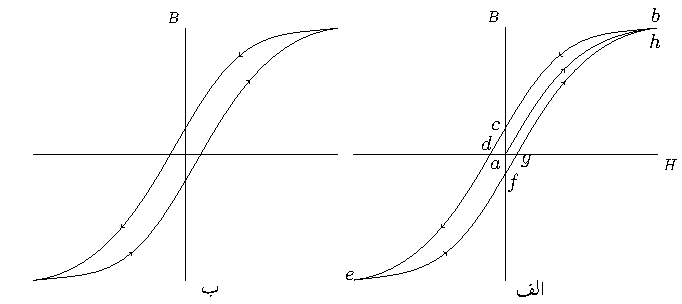
\includegraphics{figMagneticCircuitsBrillouinFunctionHysterisisLoop}
\pgfmathsetmacro{\J}{0.5}
\pgfmathsetmacro{\k}{(2*\J+1)/(2*\J)}
\def\kcoth(#1){(e^(#1)+e^(-#1))/(e^(#1)-e^(-#1))}    %this gives correct answers
\def\Brillouin(#1){and(#1>-0.001, #1< 0.001)*(0)+or(#1<-0.001, #1>0.001)*(\k*(e^(\k*#1)+e^(-\k*#1))/(e^(\k*#1)-e^(-\k*#1))-1/(2*\J)*(e^(#1/(2*\J))+e^(-#1/(2*\J)))/(e^(#1/(2*\J))-e^(-#1/(2*\J))))}    %this is correct 
%================
\begin{subfigure}{0.45\textwidth}
\centering
\begin{tikzpicture}
	\begin{axis}[small,  axis lines=middle, axis line style={-},ticks=none,ylabel=$B$, xlabel=$H$,enlargelimits=true,
xlabel style={at={(current axis.right of origin)},anchor=north},
 ylabel style={at={(current axis.above origin)},anchor=east},]
\pgfmathsetmacro{\ka}{0.5}
\pgfmathsetmacro{\kaa}{0.51}
\pgfmathsetmacro{\kpi}{2}
\addplot[ domain=0:\kpi]{\Brillouin(x)}node[pos=0,shift={(-1ex,-1ex)}]{$a$}node[pos=1,above]{$b$};
\addplot[ domain=\kpi:-\kpi]{0.2*cos(x*90/\kpi)^2+\Brillouin(x)}node[pos=0.5,above left,xshift=0.5ex]{$c$}node[pos=0.55,above,xshift=-0.5ex]{$d$}node[pos=1,left]{$e$};
\addplot[domain=-\kpi:0]{-0.15*cos(x*90/\kpi)^2+\Brillouin(x)}node[pos=1,below right,xshift=-0.5ex]{$f$};
\addplot[domain=0:\kpi]{-0.15*cos(x*90/\kpi)^2+\Brillouin(x)-0.02*(-1+e^(x/2))}node[pos=0.1,below right,xshift=-0.5ex]{$g$}node[pos=1,below]{$h$};
%arrows
\node[](a) at (axis cs:\ka,{\Brillouin(\ka)}){};
\node[](b) at (axis cs:\kaa,{\Brillouin(\kaa)}){};
\draw[-stealth](a)--(b);
%
\node[](bb) at (axis cs:\ka,{0.2*cos(\ka*90/\kpi)^2+\Brillouin(\ka)}){};
\node[](cc) at (axis cs:\kaa,{0.2*cos(\kaa*90/\kpi)^2+\Brillouin(\kaa)}){};
\draw[-stealth](cc)--(bb);
%
\node[](c) at (axis cs:-\ka,{0.2*cos(-\ka*90/\kpi)^2+\Brillouin(-\ka)}){};
\node[](d) at (axis cs:-\kaa,{0.2*cos(-\kaa*90/\kpi)^2+\Brillouin(-\kaa)}){};
\draw[-stealth](c)--(d);
%
\node[](ee) at (axis cs:-\ka,{-0.15*cos(-\ka*90/\kpi)^2+\Brillouin(-\ka)}){};
\node[](dd) at (axis cs:-\kaa,{-0.15*cos(-\kaa*90/\kpi)^2+\Brillouin(-\kaa)}){};
\draw[-stealth](dd)--(ee);
%
\node[](f) at (axis cs:\ka,{-0.15*cos(\ka*90/\kpi)^2+\Brillouin(\ka)}){};
\node[](h) at (axis cs:\kaa,{-0.15*cos(\kaa*90/\kpi)^2+\Brillouin(\kaa)}){};
\draw[-stealth](f)--(h);
%\draw(axis cs:0,0)node[below left]{$a$};
\end{axis}
\end{tikzpicture}%
\caption{}
\end{subfigure}%
\begin{subfigure}{0.45\textwidth}
\centering
\begin{tikzpicture}
\begin{axis}[small,  axis lines=middle, axis line style={-},ticks=none,ylabel=$B$, xlabel=$H$,enlargelimits=true,
xlabel style={at={(current axis.right of origin)},anchor=north}, ylabel style={at={(current axis.above origin)},anchor=east},]
\pgfmathsetmacro{\ka}{1}
\pgfmathsetmacro{\kaa}{1.1}
\pgfmathsetmacro{\kb}{-1}
\pgfmathsetmacro{\kbb}{-1.1}
\pgfmathsetmacro{\kpi}{2}
\addplot[ domain=\kpi:-\kpi]{0.2*cos(x*90/\kpi)^2+\Brillouin(x)};
\addplot[domain=-\kpi:\kpi]{-0.2*cos(x*90/\kpi)^2+\Brillouin(x)};
%arrows
\node[](a) at (axis cs:\ka,{0.2*cos(\ka*90/\kpi)^2+\Brillouin(\ka)}){};
\node[](b) at (axis cs:\kaa,{0.2*cos(\kaa*90/\kpi)^2+\Brillouin(\kaa)}){};
\node[](d) at (axis cs:\kb,{-0.2*cos(\kb*90/\kpi)^2+\Brillouin(\kb)}){};
\node[](c) at (axis cs:\kbb,{-0.2*cos(\kbb*90/\kpi)^2+\Brillouin(\kbb)}){};
\draw[-stealth](b)--(a);
\draw[-stealth](c)--(d);
\end{axis}
\end{tikzpicture}
\caption{}
\end{subfigure}
\caption{$B-H$   خطوط یا مقناطیسی چال کے دائرے۔}
\label{شکل_مقناطیسی_چال}
\end{figure}


مقناطیسی مادہ کی \عددیء{B} اور \عددیء{H} کا تعلق  ترسیم کی صورت میں پیش کیا جاتا ہے۔ لوہا نما مقناطیسی مادے کی \عددیء{B-H}  ترسیم شکل \حوالہ{شکل_مقناطیسی_چال}-الف میں دکھائی گئی ہے۔ایک لوہا نما مقناطیسی مادہ جس میں  مقناطیسی اثر نہیں پایا جاتا ہو کو نقطہ \عددیء{a} سے ظاہر کیا گیا ہے۔اس نقطہ پر درج ذیل ہوں گے۔
\begin{gather}
\begin{aligned}
H_a&=0\\
B_a&=0
\end{aligned}
\end{gather}

مقناطیسی مادہ کو لچھے میں رکھ کر اس پر مقناطیسی دباو لاگو کیا جا سکتا ہے۔ مقناطیسی میدان کی شدت \عددیء{H}  لاگو کرنے سے لوہا نما مقناطیسی مادے میں کثافت مقناطیسی بہاو  \عددیء{B} پیدا ہو گا۔میدانی شدت بڑھانے سے کثافت مقناطیسی بہاو بھی بڑھے گا۔ \عددیء{a} سے شروع ہوتا ہوا   تیردار قوس اس عمل کو ظاہر کرتا ہے۔میدانی شدت کو نقطہ \عددیء{b}  تک بڑھایا گیا ہے جہاں  \عددیء{H_b} اور \عددیء{B_b} ہوں گے۔


نقطہ \عددیء{b} تک پہنچنے کے بعد میدانی شدت کم کرتے ہوئے دیکھا گیا ہے کہ واپسی  قوس ایک مختلف راستہ اختیار کرتا ہے۔یوں نقطہ  \عددیء{b} سے میدانی شدت کم کرتے ہوئے صفر کرنے سے  لوہا نما مادہ کی کثافتِ مقناطیسی بہاو کم ہو کر نقطہ \عددیء{c} پر آن پہنچتا ہے۔نقطہ \عددیء{b} سے نقطہ \عددیء{c} تک تیردار قوس اس عمل کو ظاہر کرتا ہے۔نقطہ \عددیء{c} پر بیرونی میدانی شدت صفر ہے لیکن لوہا نما مادے کی کثافتِ مقناطیسی بہاو صفر نہیں ہے۔یہ مادہ ایک مقناطیس بن گیا ہے جس کی کثافتِ مقناطیسی بہاو  \عددیء{B_c} ہے۔اس مقدار کو \اصطلاح{بقایا کثافتِ مقناطیسی بہاو}\فرہنگ{کثافت مقناطیسی بہاو!بقایا}\فرہنگ{magnetic flux!residual}\حاشیہب{residual magnetic flux}  کہتے ہیں۔مصنوعی مقناطیس اسی طرح بنایا جاتا ہے۔

نقطہ \عددی{c} سے میدانی شدت منفی رخ  بڑھانے سے  \عددیء{B} کم ہوتے ہوتے آخر کار ایک مرتبہ دوبارہ صفر ہو جائے گا۔اس نقطہ کو \عددیء{d} سے ظاہر کیا گیا ہے۔مقناطیسیت ختم کرنے کے لئے درکار میدانی شدت کی مقدار  \عددیء{\abs{H_d}} کو مقناطیسیت ختم کرنے والی شدت یا مختصراً \اصطلاح{خاتم شدت}\فرہنگ{مقناطیس!خاتم شدت}\حاشیہب{coercivity}\فرہنگ{coercivity} کہتے ہیں۔

منفی رخ  میدانی شدت مزید بڑھانے سے  نقطہ \عددیء{e} حاصل ہو گا۔ اس کے بعد منفی رخ  کی میدانی شدت کی مطلق قیمت کم کرنے سے  نقطہ \عددیء{f} حاصل ہو گا جہاں میدانی شدت صفر ہونے کے باوجود کثافتِ مقناطیسی بہاو صفر نہیں ہے۔اس نقطہ پر لوہا نما مادہ اُلٹ رخ مقناطیس بن چکا ہے اور \عددیء{B_f} بقایا کثافتِ مقناطیسی بہاو ہے۔اسی طرح اس رخ مقناطیسیت ختم کرنے کی شدت \عددیء{\abs{H_g}} ہے۔میدانی شدت بڑھاتے ہوئے نقطہ \عددی{b} کی بجائے   نقطہ \عددیء{h} حاصل ہو گا۔

برقی شدت کو متواتر اسی طرح پہلے ایک رخ اور پھر مخالف (دوسری) رخ  ایک خاص حد تک پہنچانے سے  آخر کار \عددیء{B-H}  منحنی کا ایک بند دائرہ حاصل ہو گا جسے شکل \حوالہ{شکل_مقناطیسی_چال}-ب میں دکھایا گیا ہے۔اس دائرہ پر خلاف گھڑی سفر ہو گا۔شکل \حوالہ{شکل_مقناطیسی_چال}-ب کو  \اصطلاح{مقناطیسی چال} کا دائرہ\فرہنگ{مقناطیس!چال کا دائرہ}\حاشیہب{hysteresis loop}\فرہنگ{hysteresis loop}  کہتے ہیں۔

\begin{figure}
\centering
%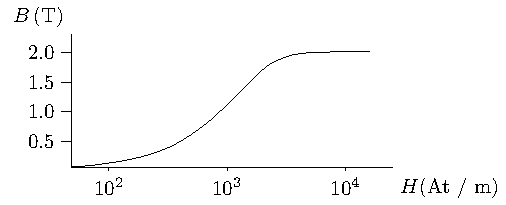
\includegraphics{figMagneticCircuitsM5curve}
\begin{tikzpicture}
\begin{semilogxaxis}[small,axis lines*=middle,xlabel={$H(\si{\ampere t\per\meter})$},ylabel={$B(\si{\tesla})$},xlabel style={at={(current axis.right of origin)},anchor=west},ylabel style={rotate={-90},at={(current axis.above origin)},anchor=south west}]
\addplot [mark=none]coordinates {
(2,0.04)
(3,0.095)
(4,0.16)
(5,0.24)
(6,0.33)
(7,0.44)
(8,0.56)
(9,0.7)
(10,0.835)
(11.22,1)
(12.59,1.1)
(14.96,1.2)
(17.78,1.3)
(20,1.34)
(23.77,1.4)
(30,1.48)
(40,1.54)
(50,1.58)
(60,1.601)
(70,1.626)
(80,1.64)
(90,1.655)
(100,1.662)
(200,1.72)
(300,1.752)
(400,1.78)
(500,1.8)
(600,1.81)
(700,1.824)
(800,1.835)
(900,1.846)
(1000,1.852)
(2000,1.9)
(10000,2)
(40000,2.06)
(70000,2.08)
};
\end{semilogxaxis}
\end{tikzpicture}%
\caption{فولاد $M5$ کی $0.3048$ ملی میٹر موٹی پتری کی ترسیم۔ میدانی شدت کا پیمانہ لاگ ہے۔}
\label{شکل_مقناطیسی_ادوار_ایم_پانچ_پتری_کا_خط}
\end{figure}

مختلف \عددیء{H} کے لئے  شکل \حوالہ{شکل_مقناطیسی_چال}-ب حاصل کر کے ایک ہی کاغذ پر کھینچنے کے بعد ان تمام کے  \عددیء{b} نقطے جوڑنے سے شکل \حوالہ{شکل_مقناطیسی_ادوار_ایم_پانچ_پتری_کا_خط} میں دکھائی گئی \عددیء{B-H} ترسیم حاصل ہو گی۔ ٹرانسفارمروں میں استعمال ہونے والی  \عددیء{0.3048}  ملی میٹر موٹی \عددیء{M5} قالبی  پتری کی \عددیء{B-H} ترسیم شکل \حوالہ{شکل_مقناطیسی_ادوار_ایم_پانچ_پتری_کا_خط} میں  دکھائی گئی ہے۔ اس ترسیم میں موجود مواد جدول \حوالہ{جدول_مقناطیسی_ادوار_کثافت_بہاو_بالمقابل_شدت}  میں بھی دیا گیا ہے۔عموماً مقناطیسی مسائل حل کرتے ہوئے شکل \حوالہ{شکل_مقناطیسی_چال} کی جگہ شکل \حوالہ{شکل_مقناطیسی_ادوار_ایم_پانچ_پتری_کا_خط} طرز  کی ترسیم استعمال کی جاتی ہے۔دھیان رہے کہ اس ترسیم میں \عددیء{H}  کا پیمانہ \اصطلاح{لاگ}\حاشیہب{log}  ہے۔

لوہا نما مقناطیسی مادے  پر لاگو مقناطیسی شدت بڑھانے سے کثافتِ مقناطیسی بہاو بڑھنے کی شرح بتدریج کم ہوتی جاتی ہے حتیٰ کہ آخر کار یہ شرح  خلاء کی شرح  \عددیء{\mu_0} کے برابر ہو جاتی ہے \عددی{(\tfrac{\Delta B}{\Delta H}= \mu_0)}۔
اس اثر کو \اصطلاح{سیرابیت}\فرہنگ{سیرابیت}\حاشیہب{saturation}\فرہنگ{saturation} کہتے ہیں جو  شکل \حوالہ{شکل_مقناطیسی_ادوار_ایم_پانچ_پتری_کا_خط}  میں واضح ہے۔

شکل \حوالہ{شکل_مقناطیسی_چال} سے واضح ہے کہ \عددیء{H} کی کسی بھی قیمت پر \عددیء{B} کی  دو ممکنہ قیمتیں ہوں گی۔ بڑھتے مقناطیسی بہاو کی صورت میں ترسیم میں نیچے سے اُوپر جانے والی منحنی \عددیء{B} اور \عددیء{H} کا تعلق پیش کرے گی جبکہ گھٹتے ہوئے مقناطیسی بہاو کی صورت میں  اوپر سے نیچے جانے والی منحنی اس تعلق کو پیش کرے  گی۔  چونکہ \عددیء{\mu=B/H} ہے  لہٰذا \عددیء{B} کی  مقدار تبدیل ہونے سے \عددیء{\mu} کی قیمت  بھی تبدیل ہو گی۔ باوجود اس کے ہم مقناطیسی ادوار میں  \عددیء{\mu} کو ایک مستقل تصور کرتے ہیں۔ ایسا کرنے سے نتائج پر عموماً زیادہ اثر انداز نہیں ہوتا ہے۔
%
\ابتدا{مثال}
شکل \حوالہ{شکل_مقناطیسی_ادوار_ایم_پانچ_پتری_کا_خط}  یا اس کے مساوی جدول \حوالہ{جدول_مقناطیسی_ادوار_کثافت_بہاو_بالمقابل_شدت} میں دی گئی مواد  استعمال کرتے ہوئے شکل \حوالہ{شکل_مقناطیسی__کثافت_مقناطیسی_بہاو_اور_شدت}  کی خلاء میں ایک ٹسلا اور دو ٹسلا کثافت  مقناطیسی بہاو حاصل کرنے کے لئے درکار برقی رو معلوم کریں۔درج ذیل معلومات استعمال کریں۔ قالب اور خلاء کا رقبہ عمودی تراش ایک دوسرے جتنا لیں۔
\begin{align*}
b=\SI{5}{\centi\meter},w=\SI{4}{\centi\meter},l_a=\SI{3}{\milli\meter},l_c=\SI{30}{\centi\meter},N=1000
\end{align*}


حل:\quad
 ایک ٹسلا کے لئے۔\\
 جدول \حوالہ{جدول_مقناطیسی_ادوار_کثافت_بہاو_بالمقابل_شدت} کے تحت قالب میں \عددیء{1} ٹسلا  کے لئے  قالب کو \عددیء{11.22}  ایمپیئر-چکر فی  میٹر قیمت کی شدت \عددیء{H}  درکار ہو گی۔یوں \عددیء{30} سم لمبے قالب کو \عددیء{0.3\times 11.22=3.366}  ایمپیئر چکر درکار ہوں گے۔

خلاء کو درج ذیل ایمپیئر-چکر فی میٹر شدت درکار ہے۔
\begin{align*}
H=\frac{B}{\mu_0}=\frac{1}{4\pi 10^{-7}}=\num{795671}
\end{align*}
یوں \عددیء{ 3 } ملی میٹر  خلاء کو \عددیء{0.003 \times 795671=2387} ایمپیئر چکر درکار ہوں گے۔ کُل ایمپیئر-چکر ان دونوں کا مجموعہ \عددیء{3.366+2387=2390.366} ہو گا جس سے  درج ذیل حاصل ہوتا ہے۔
\begin{align*}
i=\frac{2390.366}{1000}=\SI{2.39}{\ampere}
\end{align*}	

حل: دو ٹسلا کے لئے۔\\
جدول \حوالہ{جدول_مقناطیسی_ادوار_کثافت_بہاو_بالمقابل_شدت} کے تحت قالب میں \عددیء{2} ٹسلا  کثافت کے لئے  قالب کو \عددیء{10000} ایمپیئر-چکر فی میٹر \عددیء{H} درکار ہو گی۔یوں \عددیء{30} سم  قالب کو \عددیء{0.3 \times 10000=3000} ایمپیئر چکر درکار ہوں گے۔خلاء کو
\begin{align*}
H=\frac{B}{\mu_0}=\frac{2}{4\pi 10^{-7}}=\num{1591342}
\end{align*}
ایمپیئر-چکر فی میٹر درکار ہیں لہٰذا \عددیء{3} ملی میٹر لمبی خلاء کو  \عددیء{0.003 \times 1591342=4774}  ایمپیئر چکر درکار ہوں گے۔یوں کُل ایمپیئر-چکر \عددیء{3000+4774=7774} ہیں جن سے  درج ذیل حاصل کیا جا سکتا ہے۔
\begin{align*}
i=\frac{7774}{1000}=\SI{7.774}{\ampere}
\end{align*}

اس مثال میں مقناطیسی سیرابیت  واضح ہے۔ 
\انتہا{مثال}
%
\begin{table}
\begin{tabular}{l l l l   l l l l   l l l l}
$H$&$B$&$H$&$B$&$H$&$B$&$H$&$B$&$H$&$B$&$H$&$B$\\
\midrule
9000&1.998&1000&1.852&           200&1.720 &30&1.480               &9&0.700&  0&0.000    \\
10000&2.000&2000&1.900&         300&1.752 &40&1.540           &10&0.835&  2&0.040    \\
20000&2.020&3000&1.936&         400&1.780 &50&1.580          &11.22&1.000&  3&0.095    \\
30000&2.040& 4000&1.952&        500&1.800 &60&1.601         &12.59&1.100 &  4&0.160    \\
40000&2.048&5000&1.968&         600&1.810 &70&1.626          &14.96&1.200&   5&0.240    \\
50000&2.060&6000&1.975&         700&1.824 &80&1.640         &17.78&1.300&  6&0.330    \\
60000&2.070&7000&1.980&         800&1.835  &90&1.655         &20&1.340&  7&0.440    \\
 70000&2.080&8000&1.985&        900&1.846 &100&1.662          &23.77&1.400& 8&0.560    \\
\bottomrule
\end{tabular}
\caption{مقناطیسی بہاو بالمقابل شدت}
\label{جدول_مقناطیسی_ادوار_کثافت_بہاو_بالمقابل_شدت}
\end{table}
%

\حصہ{ہیجان شدہ لچھا}
بدلتا رو بجلی میں برقی دباو اور مقناطیسی بہاو عموماً سائن نما ہوتے ہیں جن کا وقت کے ساتھ تعلق \عددیء{\sin \omega t} یا \عددیء{\cos \omega t} ہو گا۔ اس حصہ میں بدلتا رو سے لچھا ہیجان کرنا اور اس سے نمودار ہونے والی برقی توانائی  کے ضیاع  پر تذکرہ  کیا جائے گا۔  قالب میں کثافت مقناطیسی بہاو
\begin{align}
B=B_0 \sin \omega t
\end{align}
کی صورت میں قالب میں درج ذیل بدلتا مقناطیسی بہاو \عددیء{\varphi} پیدا ہو گا۔
\begin{align}
\varphi=A_c B=A_c B_0 \sin \omega t=\phi_0 \sin \omega t
\end{align}
اس مساوات میں مقناطیسی بہاو کا حیطہ  \عددیء{\phi_0}، کثافت مقناطیسی بہاو کا حیطہ \عددیء{B_0}، قالب کا رقبہ عمودی تراش  \عددیء{A_c} (جو ہر مقام پر یکساں ہے)، زاویائی تعدد  \عددیء{\omega = 2 \pi f} اور تعدد \عددیء{f}  ہے۔

فیراڈے کے قانون  (مساوات \حوالہ{مساوات_مقناطیسی_دور_فیراڈے_قانون})  کے تحت یہ مقناطیسی بہاو  لچھے میں \عددیء{e(t)} \اصطلاح{امالی برقی دباو}\فرہنگ{امالی!برقی دباو}\حاشیہب{induced voltage}\فرہنگ{induced voltage}  پیدا کرے گا
\begin{gather}
\begin{aligned}
e(t)&=\frac{\partial \lambda}{\partial t}\\
&=\omega N \phi_0 \cos \omega t \\
&=\omega N A_c B_0 \cos \omega t\\
&=E_0 \cos \omega t
\end{aligned}
\end{gather}
جہاں حیطہ \عددی{E_0} درج ذیل ہے۔
\begin{align}
E_0=\omega N \phi_0=2 \pi f N A_c B_0
\end{align}

ہم بدلتے رو مقداروں کے مربع کی اوسط کے جذر  میں دلچسپی رکھتے ہیں جو ان مقداروں کی \اصطلاح{موثر}\فرہنگ{موثر}\حاشیہب{root mean square, rms}\فرہنگ{rms} قیمت ہوتی ہے۔ جیسا صفحہ \حوالہصفحہ{مساوات_بنیادی_سائن_نما_کی_موثر_قیمت} پر مساوات \حوالہ{مساوات_بنیادی_سائن_نما_کی_موثر_قیمت}  میں دیکھا گیا،  سائن نما  موج کی موثر قیمت موج کے حیطہ کی  \عددیء{1/\sqrt{2}} گنّا ہو گی  لہٰذا امالی برقی دباو کی موثر قیمت \عددی{E_{rms}} درج ذیل ہو گی۔
\begin{align}\label{مساوات_مقناطیسی_دور_پیدا_دباو_موثر_قیمت}
E_{rms}=\frac{E_0}{\sqrt{2}}=\frac{2 \pi f N A_c B_0}{\sqrt{2}}=4.44 f N A_c B_0
\end{align}
یہ مساوات بہت اہم ہے  جس کو ہم بار بار استعمال کریں گے۔بدلتے برقی دباو یا بدلتے برقی رو کی قیمت سے مراد ان کی موثر  قیمت ہو گی۔پاکستان میں گھریلو برقی دباو کی موثر قیمت \عددیء{220} وولٹ ہے۔اس سائن نما برقی دباو کی چوٹی \عددی{\sqrt{2} \times 220=311} وولٹ ہو گی۔
%
\ابتدا{مثال}\شناخت{مثال_مقناطیسی_دور_محرک_برقی_رو_کا_گراف}
شکل \حوالہ{شکل_مقناطیسی__سادہ_مقناطیسی_دور_بغیر_درز_دوبارہ} میں لچھے کے \عددیء{27} چکر ہیں۔ قالب کی لمبائی \عددیء{30 } سم جبکہ اس کا رقبہ عمودی تراش \عددیء{229.253} مربع سم ہے۔لچھے  کو گھریلو \عددیء{220} وولٹ موثر برقی دباو سے ہیجان  کیا جاتا ہے۔جدول \حوالہ{جدول_مقناطیسی_ادوار_کثافت_بہاو_بالمقابل_شدت} کی مدد سے مختلف برقی دباو پر محرک برقی رو معلوم کریں اور اس کا خط کھینچیں۔

\begin{figure}
\centering
\begin{tikzpicture}
\def\height{2};
\def\width{1.5};
\def\thick{0.4};
\def\depthX{0.2};
\def\depthY{0.2};
\def\gap{0.05};
%grid
%\draw[gray,thick](0,0) grid (5,3);
%\draw[gray,thin,xstep=0.1,ystep=0.1](0,0) grid (5,3);
%going clockwise from origin
\draw(0,0)--++(0,\height)--++(\width,0)--++(0,-\height)--cycle;
\draw(0,0)++(\thick,\thick)--++(0,\height-2*\thick)--++(\width-2*\thick,0)--++(0,-\height+2*\thick)--cycle;
%
\draw(\thick,\thick)--++(\depthX,\depthY) --++(0,\height-2*\thick-\depthY);
\draw(\thick,\thick)--++(\depthX,\depthY) --++(\width-2*\thick-\depthX,0);
\draw(0,\height)--++(\depthX,\depthY)--++(\width,0)--++(-\depthX,-\depthY);
\draw(\width,0)--++(\depthX,\depthY)--++(0,\height)--++(-\depthX,-\depthY);
%
\draw (0.6,1.4) to [out=45,in=0] (0.2,1.5) to [short,i_<=$i$] (-1,1.5) node[left]{$+$};
\foreach \l in {1.4,1.2,1}{
\draw (0,\l) to [out=-135,in=45] (0.6,\l-0.2);
}
\draw (0,0.8) to (-1,0.8)node[left]{$-$};
%turns
\node at (0,1.15)[left]{$\tau=N i$};
\end{tikzpicture}%
\caption{سادہ مقناطیسی دور (مثال \حوالہ{مثال_مقناطیسی_دور_محرک_برقی_رو_کا_گراف})۔}
\label{شکل_مقناطیسی__سادہ_مقناطیسی_دور_بغیر_درز_دوبارہ}
\end{figure}
حل:\quad
گھریلو برقی دباو \عددیء{50} ہرٹز کی سائن نما موج ہو گی۔
\begin{align}
v=\sqrt{2} \times 220 \cos (2 \pi  50 t)
\end{align}
مساوات \حوالہ{مساوات_مقناطیسی_دور_پیدا_دباو_موثر_قیمت}  کی مدد سے ہم کثافتِ مقناطیسی بہاو کی چوٹی حاصل کرتے ہیں۔
\begin{align}
B_0=\frac{220}{4.44 \times 50 \times 27 \times 0.0229253}=\SI{1.601}{\tesla}
\end{align}
یوں قالب میں کثافتِ مقناطیسی بہاو کا حیطہ  \عددیء{1.601}  ہو گا اور   قالب میں کثافتِ مقناطیسی بہاو کی مساوات درج ذیل ہو گی۔
\begin{align}\label{مساوات_مقناطیسی_دور_سائن_نما_کثافت_بہاو}
B=1.601 \sin \omega t
\end{align}
ہم جدول کی مدد سے   \عددی{0} اور \عددیء{1.601} ٹسلا کے بیچ  مختلف قیمتوں پر درکار محرک برقی رو \عددیء{i_{\phi}} معلوم کرنا چاہتے ہیں۔ہم مختلف \عددیء{B} پر جدول \حوالہ{جدول_مقناطیسی_ادوار_کثافت_بہاو_بالمقابل_شدت} سے قالب کی \عددیء{H} حاصل کریں گے جو  ایک میٹر لمبی قالب کے لئے درکار ایمپیئر-چکر ہوں گے۔اس سے \عددیء{30} سم لمبی قالب کے لئے درکار ایمپیئر-چکر  دریافت کر کے برقی رو حاصل کریں گے۔

%
\begin{table}
\begin{tabular}{l l l l l | l l l l l}
$i_{\varphi}=\frac{0.3 H}{27}$&$0.3H$&$H$&$B$&$\omega t$&$i_{\varphi}=\frac{0.3 H}{27}$&$0.3H$&$H$&$B$&$\omega t$\\
\midrule
0.000&0.000&0&0.000&0.000&0.125&3.366&11.22&1.000&0.675\\
0.022&0.600&2&0.040&0.025&0.140&3.777&12.59&1.100&0.757\\
0.033&0.900&3&0.095&0.059&0.166&4.488&14.96&1.200&0.847\\
0.044&1.200&4&0.160&0.100&0.198&5.334&17.78&1.300&0.948\\
0.056&1.500&5&0.240&0.150&0.222&6.000&20&1.340&0.992\\
0.067&1.800&6&0.330&0.208&0.264&7.131&23.77&1.400&1.064\\
0.078&2.100&7&0.440&0.278&0.333&9.000&30&1.480&1.180\\
0.089&2.400&8&0.560&0.357&0.444&12.000&40&1.540&1.294\\
0.100&2.700&9&0.700&0.453&0.556&15.000&50&1.580&1.409\\
0.111&3.000&10&0.835&0.549&0.667&18.000&60&1.601&1.571\\
\bottomrule
\end{tabular}
\caption{محرک برقی رو}
\label{جدول_مقناطیسی_ادوار_محرک_برقی_رو_بالمقابل_کثافت_بہاو}
\end{table}
%
\begin{figure}
\centering
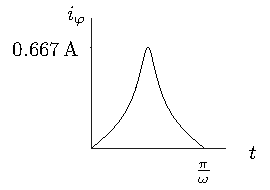
\includegraphics{figExcitationCurrentFromBHbrillouinCurveNeglectingHysterisisA}
\caption{$M5$ پتری کے قالب میں $1.6$ ٹسلا تک ہیجان پیدا کرنے کے لئے درکار ہیجان انگیز برقی رو۔}
\label{شکل_مقناطیسی_ادوار_ہیجان_رو_چال_نظرانداز}
\end{figure}

جدول \حوالہ{جدول_مقناطیسی_ادوار_محرک_برقی_رو_بالمقابل_کثافت_بہاو}  مختلف کثافتِ مقناطیسی بہاو کے لئے درکار محرک برقی رو دیتی ہے۔جدول میں  ہر \عددیء{B} کی قیمت پر  \عددیء{t} کو مساوات \حوالہ{مساوات_مقناطیسی_دور_سائن_نما_کثافت_بہاو}   سے حاصل کیا گیا ہے۔محرک برقی رو بالمقابل \عددیء{t} کا خط شکل \حوالہ{شکل_مقناطیسی_ادوار_ہیجان_رو_چال_نظرانداز} میں دیا گیا ہے۔
\انتہا{مثال}
%
برقی لچھے میں برقی دباو سے ہیجان پیدا کیا جاتا ہے۔ہیجان شدہ لچھا میں گزرتے برقی رو \عددیء{i_{\varphi}} کی بنا  قالب میں مقناطیسی بہاو پیدا ہو گا۔ اس برقی رو \عددیء{i_{\varphi}} کو \اصطلاح{ہیجان انگیز برقی رو}\فرہنگ{برقی رو!ہیجان انگیز}\حاشیہب{excitation current}\فرہنگ{excitation current}  کہتے ہیں۔

مثال \حوالہ{مثال_مقناطیسی_دور_محرک_برقی_رو_کا_گراف} میں ہیجان انگیز برقی رو معلوم کی گئی جسے شکل \حوالہ{شکل_مقناطیسی_ادوار_ہیجان_رو_چال_نظرانداز} میں دکھایا گیا۔اسے حاصل کرتے وقت \اصطلاح{مقناطیسی چال}\فرہنگ{مقناطیسی چال}\حاشیہب{hysteresis} کو نظر انداز کیا گیا۔شکل \حوالہ{شکل_مقناطیسی_ادوار_ہیجان_رو_بشمول_اثر_چال} میں ہیجان انگیز برقی رو \عددیء{i_\varphi} دکھائی گئی ہے جو مقناطیسی چال کو مدِ نظر رکھ کر حاصل کی گئی ہے۔ اس کو سمجھنا ضروری ہے۔
\begin{figure}
\centering
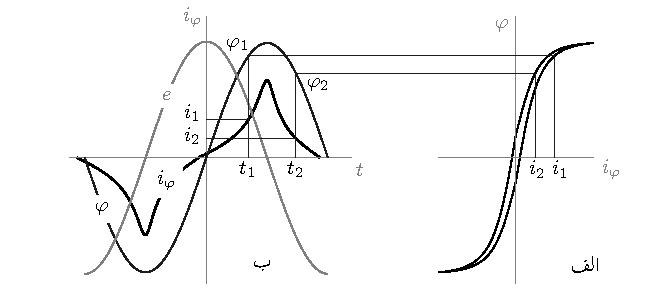
\includegraphics{figExcitationCurrentFromBHbrillouinCurveA}
\caption{ہیجان انگیز برقی رو۔}
\label{شکل_مقناطیسی_ادوار_ہیجان_رو_بشمول_اثر_چال}
\end{figure}
%
\begin{figure}
%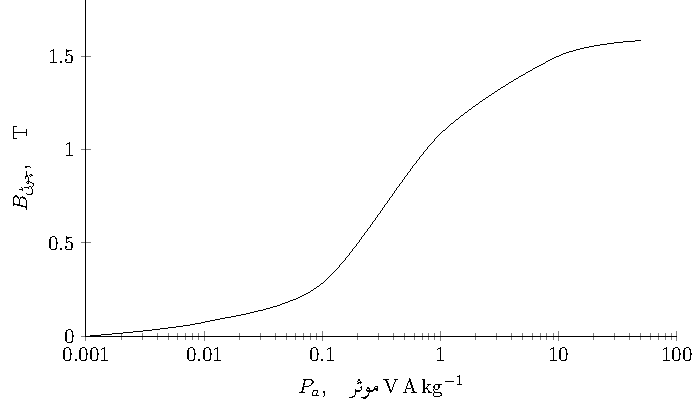
\includegraphics{figMagneticCircuitsVoltAmperePerKgVersusFluxDensity}
\pgfmathsetmacro{\radX}{1.8}
 \pgfmathsetmacro{\radY}{0.4}
\pgfmathsetmacro{\thetaStart}{0} 
\pgfmathsetmacro{\thetaEnd}{180}
\begin{tikzpicture}[yscale=0.75]
%grid
%\draw[gray,thick] (-4*\radX,-4*\radX) grid (4*\radX,4*\radX);
%\draw[gray,thin,xstep=0.1,ystep=0.1] (-4*\radX,-4*\radX) grid (4*\radX,4*\radX);
%axis
\begin{semilogxaxis}[x=2cm,
    log basis x=10,
    log ticks with fixed point,
ymax=1.8,
xmax=100,
axis x line=bottom,
axis y line=left,
axis line style=-,
xlabel={$P_{a,  \textup{موثر}}\,  (\si{\volt\ampere\per\kilogram})$},
ylabel={$B_{\textup{چوٹی}}\, (\si{\tesla})$},
    ]
%{(-3,0) (-2,0.09) (-1,0.34) (0,1.3) (1,1.8) (1.7,1.9)}
  \addplot [smooth]coordinates  {(0.001,0) (0.01,0.075) (0.1,0.283) (1,1.083) (10,1.5) (50,1.583)};
  \end{semilogxaxis}
%
% {(0.001,0) (0.01,0.09) (0.1,0.34) (1,1.3) (10,1.8) (50,1.9)} the flux is multiplied by 50/60 to get data for 50 Hz
\end{tikzpicture}%
\caption{پچاس ہرٹز پر \عددیء{0.3} ملی میٹر موٹی پتری کے لئے درکار موثر وولٹ-امپیئر فی کلوگرام قالب}
\label{شکل_مقناطیسی_دور_درکار_ہیجان_وولٹ_ایمپیئر}
\end{figure}

شکل \حوالہ{شکل_مقناطیسی_ادوار_ہیجان_رو_بشمول_اثر_چال}-الف میں  مقناطیسی چال کا دائرہ دکھایا گیا  ہے۔درج ذیل تعلقات کی بنا مقناطیسی چال کے  خط کو \عددیء{\varphi-i_{\varphi}} کا خط لکھا جا سکتا ہے۔
\begin{gather}
\begin{aligned}
H l& =N i\\
\varphi&=B A_c
\end{aligned}
\end{gather}
قالب میں سائن نما مقناطیسی بہاو \عددیء{\varphi}  کو شکل \حوالہ{شکل_مقناطیسی_ادوار_ہیجان_رو_بشمول_اثر_چال}-ب  میں دکھایا گیا ہے۔سائن نما مقناطیسی بہاو وقت کے ساتھ تبدیل ہوتا ہے۔لمحہ \عددیء{t_1} پر اس کی قیمت  \عددیء{\varphi_1} ہو گی۔مقناطیسی بہاو \عددیء{\varphi_1} حاصل کرنے کے لئے درکار ہیجان انگیز برقی رو \عددیء{i_1} شکل-الف سے حاصل کی جا سکتی ہے۔اسی  ہیجان انگیز برقی رو کو شکل-ب میں  لمحہ \عددیء{t_1} پر دکھایا گیا ہے۔

دھیان رہے کہ لمحہ \عددیء{t_1} پر مقناطیسی بہاو بڑھ رہا ہے لہٰذا مقناطیسی چال کے خط کا درست حصہ استعمال کرنا ضروری ہے۔شکل \حوالہ{شکل_مقناطیسی_ادوار_ہیجان_رو_بشمول_اثر_چال}-الف میں  \عددیء{\varphi-i_{\varphi}}  کے خط میں گھڑی کی سوئیوں کے مخالف رخ گھومتے ہوئے یوں نیچے سے اوپر جاتا ہوا حصہ استعمال کیا گیا ہے۔شکل \حوالہ{شکل_مقناطیسی_چال}-ب میں  تیر کے نشان  مقناطیسی بہاو بڑھنے (نیچے سے اوپر) اور گھٹنے (اوپر سے نیچے) والے حصوں کی نشاندہی کرتے ہیں۔


 لمحہ \عددیء{t_2} پر مقناطیسی بہاو گھٹ رہا ہے۔اس لمحہ پر مقناطیسی بہاو \عددیء{\varphi_2} ہے اور اسے حاصل کرنے کے لئے درکار ہیجان انگیز برقی رو \عددیء{i_2} ہے۔

اسی طرح مختلف لمحات پر درکار ہیجان انگیز برقی رو حاصل کرنے سے شکل \حوالہ{شکل_مقناطیسی_ادوار_ہیجان_رو_بشمول_اثر_چال}-ب کا    \عددیء{i_{\varphi}}  خط ملتا ہے جو  غیر سائن نما ہے۔

آپ جانتے ہیں کہ  \عددیء{\varphi=\phi_0 \sin \omega t} کی صورت میں برقی دباو \عددیء{e=N \tfrac{\dif \varphi}{\dif t}=N \phi_0 \omega \cos \omega t} ہو گا۔شکل \حوالہ{شکل_مقناطیسی_ادوار_ہیجان_رو_بشمول_اثر_چال}-ب میں اس برقی دباو کو بھی دکھایا گیا ہے۔آپ دیکھ سکتے ہیں کہ برقی دباو سے  مقناطیسی بہاو \عددیء{90 \degree} تاخیر سے ہے۔

قالب میں  \عددیء{B=B_0 \sin \omega t} کی صورت میں  \عددیء{H} اور \عددیء{i_{\varphi}}  غیر سائن نما ہوں گے جن  کی موثر قیمتوں \عددیء{H_{c,rms}} اور  \عددیء{i_{\varphi,rms}} کا تعلق درج ذیل ہو گا۔
\begin{align}\label{مساوات_مقناطیسی_دور_دباو_برابر_شدت_ضرب_لمبائی}
N i_{\varphi,rms}=l_c H_{c,rms}
\end{align}
مساوات \حوالہ{مساوات_مقناطیسی_دور_پیدا_دباو_موثر_قیمت}   اور مساوات \حوالہ{مساوات_مقناطیسی_دور_دباو_برابر_شدت_ضرب_لمبائی}  سے درج ذیل حاصل ہو گا
\begin{align}\label{مساوات_مقناطیسی_دور_درکار_دباو_ضرب_رو}
E_{rms} i_{\varphi,rms}=\sqrt{2} \pi f B_0 H_{c,rms} A_c l_c
\end{align}
جہاں  \عددیء{A_c l_c} قالب کا حجم ہے۔ یوں   \عددیء{A_c l_c} حجم کے قالب  میں  \عددیء{B_0} کثافتِ مقناطیسی بہاو پیدا کرنے کے لئے درکار \عددیء{E_{rms} i_{\varphi,rms}} مساوات \حوالہ{مساوات_مقناطیسی_دور_درکار_دباو_ضرب_رو}  دے گی۔ ایک مقناطیسی قالب جس کا حجم  \عددیء{A_c l_c} اور  میکانی کثافت  \عددیء{\rho_c} ہو، کی کمیت \عددیء{m_c=\rho_c A_c l_c} ہو گی لہٰذا  ایک کلوگرام  قالب کے لئے مساوات \حوالہ{مساوات_مقناطیسی_دور_درکار_دباو_ضرب_رو} کو  درج ذیل روپ میں لکھا جا سکتا ہے۔
\begin{align}
P_a=\frac{E_{rms} i_{\varphi,rms}}{m_c}=\frac{\sqrt{2} \pi f}{\rho_c} B_0 H_{c,rms}
\end{align}
دیکھا جائے تو کسی ایک تعدد  \عددیء{f} پر \عددیء{P_a} کی قیمت صرف قالب پر اور قالب میں \عددیء{B_0} یعنی \عددیء{B_{\textup{چوٹی}}} پر منحصر ہے، چونکہ \عددیء{H_{c,rms}} خود \عددیء{B_0} پر منحصر ہے۔ یہی وجہ ہے کہ  قالب بنانے والے اکائی کمیت کے قالب میں مختلف \عددیء{B_{\textup{چوٹی}}} پیدا کرنے کے لئے درکار \عددیء{E_{rms} i_{\varphi,rms}} کی \عددیء{B_0} بالمقابل \عددیء{P_a} ترسیم مہیا کرتے ہیں۔قالب کی \عددیء{0.3} ملی میٹر موٹی پتری کے لئے ایسی ترسیم  شکل \حوالہ{شکل_مقناطیسی_دور_درکار_ہیجان_وولٹ_ایمپیئر} میں دکھائی گئی ہے۔

\باب{ٹرانسفارمر}
ٹرانسفارمر وہ آلہ ہے جو بدلتی برقی دباو تبدیل کرتا ہے۔ یہ دو یا دو سے زیادہ لچھوں پر مشتمل ہوتا ہے جو مقناطیسی قالب\فرہنگ{مقناطیسی قالب}\حاشیہب{magnetic core}\فرہنگ{core} پر لپٹے ہوتے ہیں۔یہ لچھے عموماً آپس میں جُڑے ہوئے نہیں ہوتے۔شکل \حوالہ{شکل_ٹرانسفارمر_علامت}-الف میں ٹرانسفارمر کی علامت دکھائی گئی ہے۔دو لچھوں کے درمیان متوازی لکیریں مقناطیسی قالب کو ظاہر کرتی ہیں۔

دستیاب برقی دباو\حاشیہد{بدلتی برقی دباو کی علامت میں مثبت اور منفی نشان وقت صفر پر برقی دباو کی مثبت اور منفی سرے ظاہر کرتے ہیں۔} پر ٹرانسفارمر کے ایک لچھے کو برقی طاقت فراہم کی جاتی ہے اور باقی لچھوں سے  مختلف برقی دباو پر یہی برقی طاقت حاصل کی جاتی ہے۔جس لچھے پر برقی دباو لاگو کیا جائے اسے \اصطلاح{ابتدائی لچھا}\فرہنگ{لچھا!ابتدائی}\فرہنگ{ابتدائی!لچھا}\حاشیہب{primary coil}\فرہنگ{coil!primary}  کہتے ہیں اور ٹرانسفارمر کی اس جانب کو \اصطلاح{ابتدائی جانب}\فرہنگ{ابتدائی!جانب}\حاشیہب{primary side}\فرہنگ{primary!side} کہتے ہیں۔اسی طرح جس لچھے (لچھوں) سے برقی طاقت حاصل کی جاتی ہے اسے (انہیں) \اصطلاح{ثانوی لچھا}\فرہنگ{لچھا!ثانوی}\حاشیہب{secondary coil}\فرہنگ{coil!secondary}  (لچھے) کہتے ہیں اور اس جانب کو \اصطلاح{ثانوی جانب}\فرہنگ{ثانوی جانب}\فرہنگ{side!secondary}\حاشیہب{secondary side}  کہتے ہیں۔یہ شکل کے حصہ با میں دکھایا گیا ہے۔ٹرانسفارمر کی ابتدائی جانب کو بائیں ہاتھ کی جانب اور ثانوی جانب کو دائیں ہاتھ کی جانب بنایا جاتا ہے۔
\begin{figure}
\centering
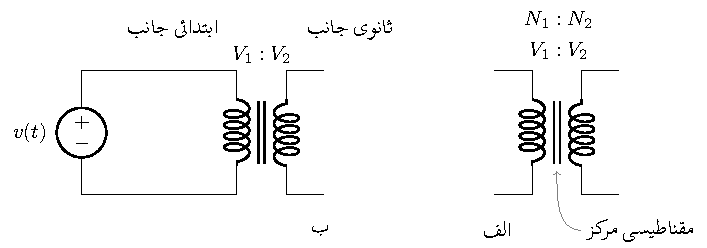
\includegraphics{figTransformersSymbol}
\caption{ٹرانسفارمر کی علامت۔}
\label{شکل_ٹرانسفارمر_علامت}
\end{figure}

بڑے ٹرانسفارمر عموماً دو ہی لچھوں پر مشتمل ہوتے ہیں۔اس کتاب میں ہم دو ہی لچھوں کے مقناطیسی قالب پر لپٹے قوی ٹرانسفارمر پر تبصرہ کریں گے۔

	ٹرانسفارمر کے کم برقی دباو کے لچھے کو \اصطلاح{کم برقی دباو کا لچھا}\فرہنگ{لچھا!کم برقی دباو}\حاشیہب{low voltage coil}\فرہنگ{coil!low voltage}  کہتے ہیں اور ٹرانسفارمر کی اس جانب کو \اصطلاح{کم برقی دباو والی جانب}  کہتے ہیں جبکہ اس کے زیادہ برقی دباو کے لچھے کو \اصطلاح{زیادہ برقی دباو کا لچھا}\فرہنگ{لچھا!زیادہ برقی دباو}\حاشیہب{high voltage coil}\فرہنگ{coil!high voltage}  کہتے ہیں اور ٹرانسفارمر کی اس جانب کو \اصطلاح{زیادہ برقی دباو والی جانب}  کہتے ہیں۔

یوں اگر ٹرانسفارمر کے کم برقی دباو کی جانب برقی دباو لاگو کیا جائے اور زیادہ برقی دباو کی جانب سے برقی دباو حاصل کیا جائے تو ٹرانسفارمر کی کم برقی دباو والی جانب کو ابتدائی جانب کہیں گے اور اس کی زیادہ برقی دباو والی جانب کو ثانوی جانب کہیں گے۔

\حصہ{ٹرانسفارمر کی اہمیت}
بدلتی رو کی برقی طاقت اتنی مقبول اس لئے ہوئی ہے کہ یہ ایک جگہ سے دوسری جگہ با آسانی اور نہایت کم برقی طاقت کی ضیاع کے ساتھ منتقل کی جا سکتی ہے۔ٹرانسفارمر کی تبادلہ برقی دباو\فرہنگ{برقی دباو!تبادلہ}\حاشیہب{voltage transformation property} کی خصوصیت ایسا کرنے میں کلیدی کردہر ادا کرتی ہے۔ یہ ایک مثال سے بہتر سمجھا جا سکتا ہے۔
%
\ابتدا{مثال}
شکل \حوالہ{شکل_ٹرانسفارمر_برقی_طاقت_منتقلی}  سے رجوع کریں۔برقی دباو اور برقی رو کی حاصلِ ضرب برقی طاقت ہوتی ہے یعنی
\begin{figure}
\centering
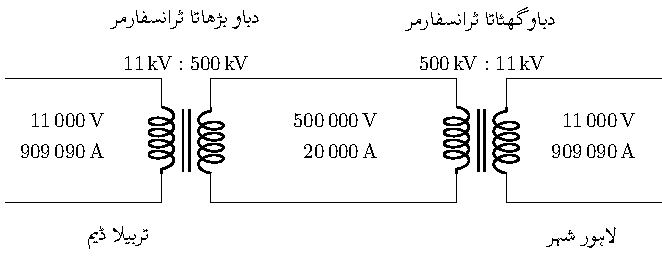
\includegraphics{figTransformersVoltageStepUpBenefits}
\caption{برقی طاقت کی منتقلی۔}
\label{شکل_ٹرانسفارمر_برقی_طاقت_منتقلی}
\end{figure}

%
\begin{align*}
p=v_1 i_1 = v_2 i_2
\end{align*}
اب تصور کریں کہ تربیلا ڈیم \عددیء{10,000,000,000} واٹ یعنی دس گیگا واٹ\حاشیہب{Giga Watt}  برقی طاقت پیدا کر رہا ہے اور اس طاقت کو لاہور\حاشیہد{ضلع صوابی میں بھی لاہور ایک تحصیل ہے لیکن اس شہر کو اتنی طاقت نہیں درکار } شہر منتقل کرنا ہے جہاں گھریلو صارفین کو یہ \عددیء{220} وولٹ پر مہیا کرنی ہے۔اگر ہم اس طاقت کو \عددیء{220}  وولٹ پر ہی منتقل کرنا چاہیں تو برقی رو
\begin{align*}
i=\frac{p}{v}=\frac{\num{10000000000}}{220}=\SI{45454545}{\ampere}
\end{align*}
ہو گی۔برقی تار میں کثافتِ برقی رو \عددیء{J_{au}} تقریباً \عددیء{5} ایمپیئر فی مربع ملی میٹر \عددیء{J_{au}=\SI{5}{\ampere \per \milli\meter \squared}}  ممکن ہوتی ہے۔یہ ایک محفوظ کثافتِ برقی رو ہے۔اگر برقی تار میں اس سے زیادہ برقی رو گزاری جائے تو اس کی مزاحمت میں برقی طاقت کے ضیاع سے یہ گرم ہو کر پگھل سکتی ہے۔ اس طرح صفحہ \حوالہصفحہ{مساوات_بنیادی_برقی_رو_کثافت} پر  مساوات \حوالہ{مساوات_بنیادی_برقی_رو_کثافت} سے برقی تار کا رقبہ عمودی تراش
\begin{align*}
A=\frac{i}{J_{au}}=\frac{45454545}{5}=\SI{9090909}{\milli\meter\squared}
\end{align*}
ہو گا۔ گول تار تصور کریں تو اس کا رداس
\begin{align*}
r=\sqrt{\frac{A}{\pi}}=\sqrt{\frac{9090909}{\pi}}=\SI{1701}{\milli\meter}=\SI{1.7}{\meter}
\end{align*}
حاصل ہوتی ہے۔آپ نے دیکھا کہ درکار برقی تار کا رداس \عددیء{1.7} میٹر ہے۔اتنی موٹی برقی تار کہیں نہیں پائی جاتی ہے\حاشیہد{آپ مانیں یا نہ مانیں، آپ نے بھی اتنی موٹی برقی تار کبھی نہیں دیکھی}۔اگر یہ تار المونیم کی بنی ہو جس کی  کثافت  \عددیء{\rho_v=\SI{2700}{\kilo\gram\per\meter\squared}} ہے تو ایک میٹر لمبی تار کی کمیت
\begin{align*}
m=2700 \times \pi \times 1.7^2 \times 1=\SI{24513}{\kilo\gram}
\end{align*}
یعنی \عددیء{24} ٹن ہو گی۔المونیم اتنی مہنگی ہے کہ اس صورت میں اتنی برقی طاقت کو لاہور پہنچانا ممکن نہیں\حاشیہد{آج کل لاہور میں لوڈ شیدنگ اس وجہ سے نہیں}۔

ڈیم پر ایک ٹرانسفارمر نسب کیا جائے جو برقی دباو کو بڑھا کر  \عددیء{\num{500000}} وولٹ یعنی \عددیء{500} کلو وولٹ  کر دے تب صرف 
\begin{align*}
i=\frac{p}{v}=\frac{\num{10000000000}}{\num{500000}}=\SI{20000}{\ampere}
\end{align*}
ایمپیئر درکار ہوں گے جس کے لئے درکار برقی تار
\begin{align*}
A&=\frac{i}{J_{au}}=\frac{\num{20000}}{5}=\SI{4000}{\milli\meter\squared}\\
r&=\sqrt{\frac{A}{\pi}}=\sqrt{\frac{4000}{\pi}}=\SI{35.7}{\milli\meter}
\end{align*}
صرف \عددیء{35} ملی میٹر رداس کی ہو گی۔
\انتہا{مثال}
%

اس مثال میں اگر تربیلا ڈیم میں نسب جنریٹر \عددیء{11000} وولٹ برقی دباو پیدا کر رہا ہو تو تربیلا ڈیم  پر نسب  ٹرانسفارمر برقی دباو کو \عددیء{11000} وولٹ سے بڑھا کر \عددیء{500} کلو وولٹ کرے گا جبکہ لاہور شہر میں نسب  ٹرانسفارمر اس برقی دباو کو \عددیء{500} کلو وولٹ سے واپس \عددیء{11000} وولٹ کر دے گا۔

اسی مثال کو مزید آگے لے جاتے ہیں۔شہر میں \عددیء{220} وولٹ کی بجائے \عددیء{11000} وولٹ صارف تک پہنچائے جائیں گے اور۔وہیں نزدیک ایک اور ٹرانسفارمر  \عددیء{11000}  وولٹ کو مزید گھٹا کر صارف کو  \عددیء{220} وولٹ فراہم کرے گی۔ 

شکل \حوالہ{شکل_ٹرانسفارمر_برقی_طاقت_منتقلی} میں ڈیم سے شہر تک کا نظام دکھایا گیا ہے جہاں ڈیم پر نسب ٹرانسفارمر کو \اصطلاح{برقی دباو بڑھاتا ٹرانسفارمر}\فرہنگ{ٹرانسفارمر!دباو بڑھاتا}\حاشیہب{step up transformer}\فرہنگ{step up transformer}  اور لاہور میں نسب ٹرانسفارمر کو \اصطلاح{برقی دباو گھٹاتا ٹرانسفارمر}\فرہنگ{ٹرانسفارمر!دباو گھٹاتا}\حاشیہب{step down transformer}\فرہنگ{step down transformer}  کہا گیا ہے۔

برقی طاقت عموماً \عددیء{11} کلو وولٹ اور  \عددیء{25} کلو وولٹ کے مابین پیدا کی جاتی ہے۔اس کی منتقلی  \عددیء{110 } کلو وولٹ اور \عددیء{1000}  کلو وولٹ کے مابین کی جاتی ہے جبکہ اس کا استعمال  \عددیء{1000} وولٹ سے کم پر کیا جاتا ہے۔

\حصہ{ٹرانسفارمر کے اقسام}
گھروں اور کارخانوں کو برقی طاقت فراہم کرنے والے ٹرانسفارمر مقناطیسی قالب پر لپٹے جاتے ہیں۔یہ عموماً  \اصطلاح{تین مرحلہ}\فرہنگ{تین مرحلہ}\حاشیہب{three phase}\فرہنگ{three phase} ہوتے ہیں۔ اور انہیں \اصطلاح{لوہے کے قالب والے تین  مرحلہ قوی ٹرانسفارمر}\حاشیہب{iron core, three phase power transformer} کہتے ہیں۔

نہایت چھوٹے ٹرانسفارمر عموماً لوہے کے قالب اور \اصطلاح{ایک مرحلہ}\فرہنگ{ایک مرحلہ}\حاشیہب{single phase}\فرہنگ{single phase} ہوتے ہیں۔یہ گھریلو استعمال کے برقی مشین، مثلاً موبائل چارجر، میں لگے ہوتے ہیں اور \عددیء{220} وولٹ سے برقی دباو مزید گھٹاتے ہیں۔

کچھ ٹرانسفارمر اس طرح بنائے جاتے ہیں کہ ان کی ثانوی جانب برقی دباو ان کی ابتدائی جانب برقی دباو کی خاص نسبت سے ہو۔یہ نسبت حاصل کرنے پر خاص توجہ دی جاتی ہے۔ انہیں  \اصطلاح{دباو کے ٹرانسفارمر}\فرہنگ{ٹرانسفارمر!برقی دباو، میٹر}\حاشیہب{potential transformer}  کہتے ہیں۔اسی طرح کچھ ٹرانسفارمر اس طرح بنائے جاتے ہیں کہ ان کی ثانوی جانب برقی رو، ابتدائی جانب برقی رو کی خاص نسبت سے ہو۔ یہ نسبت حاصل کرنے پر خاص توجہ دی جاتی ہے۔ان کو \اصطلاح{رو کے ٹرانسفارمر}\فرہنگ{ٹرانسفارمر!رو، میٹر}\حاشیہب{current transformer}  کہتے ہیں۔یہ دو قسم کے ٹرانسفارمر برقی دباو اور برقی رو ناپنے کے لئے استعمال ہوتے ہیں۔ ویسے تو ہر ٹرانسفارمر کسی نسبت سے ہی برقی دباو یا برقی رو کم یا زیادہ کرتا ہے لیکن جیسا پہلے ذکر ہوا ان دو قسم کے ٹرانسفارمروں میں کم اور زیادہ کرنے کی نسبت پر خاص توجہ رکھی جاتی ہے۔ان دو اقسام کے ٹرانسفارمروں کی برقی سکت\فرہنگ{برقی سکت}\حاشیہب{electrical rating}\فرہنگ{electrical rating} نہایت کم\حاشیہد{یہ عموماً تقریباً پچیس وولٹ-ایمپیئر سکت رکھتے ہیں۔} ہوتی ہے۔

ٹرانسفارمر کے لچھوں کے مابین مشترکہ مقناطیسی بہاو خلاء کے ذریعہ بھی ممکن ہے۔انہیں \اصطلاح{خلائی قالب ٹرانسفارمر}\فرہنگ{ٹرانسفارمر!خلائی قالب}\حاشیہب{air core transformer}\فرہنگ{transformer!air core}  کہتے ہیں۔ ایسے ٹرانسفارمر ذرائع ابلاغ\فرہنگ{ٹرانسفارمر!ذرائع ابلاغ}\حاشیہب{communication transformer}\فرہنگ{transformer!communication} کے ادوار، یعنی ریڈیو، ٹی وی وغیرہ میں پائے جاتے ہیں۔ان ٹرانسفارمروں کی علامت  شکل  الف کی طرح ہوتی ہے مگر اس میں مقناطیسی قالب ظاہر کرنے والی متوازی لکیریں نہیں ہوتیں۔

\حصہ{امالی برقی دباو}\شناخت{حصہ_ٹرانسفارمر_امالی_برقی_دباو}
اس حصے کا بنیادی مقصد بیرونی برقی دباو \عددیء{v}  اور اندرونی امالی برقی دباو  \عددیء{e} میں فرق واضح کرنا اور اس سے تعلق رکھنے والی تکنیکی اصطلاح کا تعارف کرانا ہے۔

شکل  \حوالہ{شکل_ٹرانسفارمر_بیرونی_اور_اندرونی_برقی_دباو} میں بے بوجھ\فرہنگ{بے بوجھ}\حاشیہب{unloaded} ٹرانسفارمر دکھایا گیا ہے یعنی اس کے ثانوی لچھے کو کھلے دور رکھا گیا ہے۔ابتدائی لچھے پر \عددیء{v_1} برقی دباو لاگو کرنے سے ابتدائی لچھے میں ہیجان انگیز\فرہنگ{ہیجان انگیز برقی رو}\حاشیہب{excitation current}\فرہنگ{excitation current} برقی رو \عددیء{i_{\varphi}} گزرے گی۔اس ہیجان انگیز برقی رو سے پیدا مقناطیسی دباو \عددیء{N_1 i_{\varphi}}  قالب میں مقناطیسی بہاو  \عددیء{\varphi} کو جنم دے گی۔ یہ بدلتی مقناطیسی بہاو ابتدائی لچھے میں امالی برقی  دباو \عددیء{e_1}  پیدا کرتی ہے جہاں
\begin{align}
e_1=-\frac{\dif \lambda}{\dif t}=-N_1 \frac{\dif \varphi}{\dif t}
\end{align}

 اس مساوات میں
\begin{itemize}
\item
\عددیء{\lambda} ابتدائی لچھے کی مقناطیسی بہاو کے ساتھ ارتباط بہاو ہے
\item
\عددیء{\varphi} مقناطیسی قالب میں مقناطیسی بہاو جو دونوں لچھوں میں سے گزرتی ہے
\item
\عددیء{N_1} ابتدائی لچھے کے چکر
\end{itemize}
%
\begin{figure}
\centering
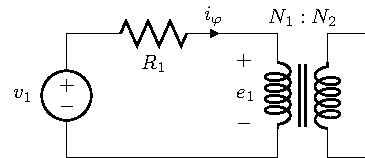
\includegraphics{figTransformersAppliedAndInducedVoltages}
\caption{بیرونی برقی دباو اور اندرونی امالی برقی دباو میں فرق۔}
\label{شکل_ٹرانسفارمر_بیرونی_اور_اندرونی_برقی_دباو}
\end{figure}

اگر اس ابتدائی لچھے کی برقی تار کی مزاحمت \عددیء{R_1} ہو تب کرخوف کے قانون برائے برقی دباو سے
\begin{align}\label{مساوات_ٹرانسفارمر_بیرونی_اندرونی_دباو_فرق}
v_1 = i_{\varphi} R_1+e_1
\end{align}

شکل میں اس مزاحمت کو ٹرانسفارمر کے باہر دکھایا گیا ہے۔اس لچھے کی رِستا متعاملہ بھی ہوتی ہے لیکن اسے یہاں نظرانداز کیا گیا ہے۔عام تر طاقت کے ٹرانسفارمر اور موٹروں  میں \عددیء{i_{\varphi} R_1} کی قیمت \عددیء{e_1} اور \عددیء{v_1} سے بہت کم ہوتی ہے لہٰذا اسے نظرانداز کیا جا سکتا ہے۔ ایسا کرنے سے ہم لکھ سکتے ہیں 
\begin{align}\label{مساوات_ٹرانسفارمر_بیرونی_اندرونی_دباو_تقریبا_برابر}
v_1 = e_1=-N_1 \frac{\dif \varphi}{\dif t}
\end{align}

مساوات \حوالہ{مساوات_ٹرانسفارمر_بیرونی_اندرونی_دباو_فرق} سے یہ ثابت ہوتا ہے کہ بیرونی لاگو برقی دباو \عددیء{v_1} اور اندرونی امالی برقی دباو \عددیء{e_1} دو علیحدہ برقی دباو ہیں۔یہ بات سمجھ لینا بہت ضروری ہے۔مساوات \حوالہ{مساوات_ٹرانسفارمر_بیرونی_اندرونی_دباو_تقریبا_برابر} کے تحت ان دو برقی دباو کی غیر سمتیں عموماً برابر ہوتی ہیں۔\حاشیہد{جس سے طلباء کو یہ غلط فہمی لاحق ہو جاتی ہے کہ یہ ایک ہی برقی دباو کے دو نام ہیں۔}اس کتاب میں عموماً مساوات \حوالہ{مساوات_ٹرانسفارمر_بیرونی_اندرونی_دباو_تقریبا_برابر}  کی طرح مساواتوں میں دائیں جانب منفی کی علامت نہیں لکھی گئی ۔عموماً برقی دباو کی قیمت درکار ہوتی ہے نا کہ اس کی علامت۔

لچھا \اصطلاح{ہیجان}\فرہنگ{ہیجان}\حاشیہب{excitation}\فرہنگ{excitation} کرنے سے مراد اس پر بیرونی برقی دباو لاگو کرنا  جبکہ لچھے پر لاگو بیرونی برقی دباو کو \اصطلاح{ہیجان انگیز برقی دباو}\فرہنگ{ہیجان انگیز!برقی دباو}\حاشیہب{excitation voltage}\فرہنگ{excitation voltage}  کہتے ہیں۔لچھے  کو \اصطلاح{ہیجان شدہ} لچھا\فرہنگ{ہیجان!لچھا}\حاشیہب{excited coil}\فرہنگ{excited coil} جبکہ اس میں رواں برقی رو کو \اصطلاح{ہیجان انگیز برقی رو}\فرہنگ{ہیجان انگیز!برقی رو}\فرہنگ{excitation current}\حاشیہب{excitation current} کہتے ہیں۔

برقی دباو عموماً لچھے سے گزرتی مقناطیسی بہاو کی تبدیلی سے حاصل کی جاتی ہے۔اگر ایسا کرتے لچھا ساکن رہے، جیسا کہ ٹرانسفارمر میں ہوتا ہے، تب حاصل برقی دباو کو \اصطلاح{امالی برقی دباو}\فرہنگ{امالی برقی دباو}\حاشیہب{induced voltage}\فرہنگ{induced voltage}  کہتے ہیں۔اگر برقی دباو کا حصول مقناطیسی میدان میں لچھے کی حرکت سے ممکن بنایا جائے تب اسے  \اصطلاح{محرک برقی دباو}\فرہنگ{محرک برقی دباو}\حاشیہب{electromotive force, emf}\فرہنگ{electromotive force}  کہتے ہیں۔یاد رہے ان برقی دباو میں کسی قسم کا فرق نہیں ہوتا۔انہیں مختلف نام صرف پہچان کی خاطر دئے جاتے ہیں۔

\حصہ{ہیجان انگیز  برقی رو اور قالبی ضیاع}
جہاں مقناطیسی قالب میں بدلتی مقناطیسی بہاو ثانوی لچھوں میں فائدہ مند برقی دباو پیدا کرتی ہے وہاں یہ مقناطیسی قالب میں نقصان دہ برقی دباو کو بھی جنم دیتی ہے جس سے مقناطیسی قالب میں \اصطلاح{بھنور نما برقی رو}\فرہنگ{بھنور نما!برقی رو}\حاشیہب{eddy currents}\فرہنگ{eddy currents} پیدا ہوتی ہے۔ اس بھنور نما برقی رو کی وجہ سے مقناطیسی قالب میں برقی طاقت کا ضیاع ہوتا ہے جسے \اصطلاح{بھنور نما برقی رو کا ضیاع}\فرہنگ{بھنور نما!ضیاع}\حاشیہب{eddy current loss}\فرہنگ{eddy current loss}  یا \اصطلاح{قالبی ضیاع}\فرہنگ{قالبی ضیاع}\حاشیہب{core loss}\فرہنگ{core loss} کہتے ہیں۔ اس برقی طاقت  کے ضیاع کو کم سے کم کرنے کیلئے مقناطیسی قالب کو  باریک لوہے کی \اصطلاح{پتریاں}\فرہنگ{پتریاں}\حاشیہب{laminations}\فرہنگ{laminations} تہہ در تہہ رکھ کر بنایا جاتا ہے۔ان پتریوں پر غیر موصل روغن\فرہنگ{روغن}\حاشیہب{enamel}\فرہنگ{enamel} کی تہہ لگائی جاتی ہے تا کہ بھنور نما برقی رو کو روکا جا سکے۔آپ دیکھیں گے کہ برقی مشین کا قالب عموماً اسی طرح بنایا جاتا ہے۔شکل \حوالہ{شکل_مقناطیسی_ادوار_ایم_پانچ_پتری_کا_خط} اور جدول \حوالہ{جدول_مقناطیسی_ادوار_کثافت_بہاو_بالمقابل_شدت}  میں \عددیء{0.3048} ملی میٹر موٹی \تحریر{M5} قالبی پتری کی \عددیء{B-H} مواد دی گئی ہے۔

قالبی پتریاں عموماً دو اشکال کی ہوتی ہیں۔یہ شکل \حوالہ{شکل_ٹرانسفارم_تہہ_در_تہہ_مرکز}-الف میں دکھایا گیا ہے۔ان کی شکل کی وجہ سے یہ \اصطلاح{ایک} شکل اور \اصطلاح{تین}\فرہنگ{ایک، تین پتریاں}\حاشیہب{E,I}\فرہنگ{E,I} شکل کی پتریاں کہلاتے ہیں۔ شکل \حوالہ{شکل_ٹرانسفارم_تہہ_در_تہہ_مرکز}-ب میں ایک اور تین  کو دو طرح آپس میں رکھا گیا ہے۔ان دو طریقوں سے انہیں تہہ در تہہ رکھا جاتا ہے۔لہٰذا اگر پہلی تہہ میں ایک دائیں جانب اور تین بائیں جانب رکھا جائے تو اس کے اوپر دوسری تہہ میں ایک کو بائیں جانب اور تین کو دائیں جانب رکھا جائے گا۔تیسری تہہ میں پھر ایک کو دائیں اور تین کو بائیں جانب رکھا جائے گا۔اسی طرح انہیں جوڑ کر شکل کے حصہ د میں دکھایا گیا قالب حاصل کیا جاتا ہے۔

\begin{figure}
\centering
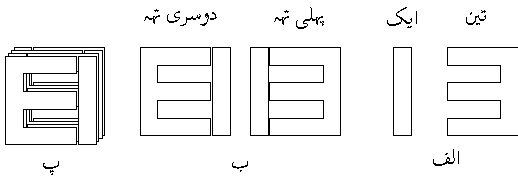
\includegraphics{figTransformersCorePlacement}
\caption{قالبی پتری کے اشکال اور ان کو تہہ در تہہ رکھنے کا طریقہ۔}
\label{شکل_ٹرانسفارم_تہہ_در_تہہ_مرکز}
\end{figure}

ہیجان انگیز برقی رو بے بوجھ اور بوجھ بردار ٹرانسفارمر میں یکساں ہوتا ہے ۔جیسا کہ پہلے بھی ذکر کیا گیا ہے، قوی ٹرانسفارمر اور موٹروں میں برقی دباو اور مقناطیسی بہاو سائن نما ہوتے ہیں جبکہ ہیجان انگیز برقی رو ان میں غیر سائن نما ہوتی ہے لہٰذا اگر
\begin{gather}
\begin{aligned}
\varphi&=\phi_0 \sin \omega t=\phi_0 \cos \left(\omega t -90\degree \right)\\
\hat{\varphi}&=\phi_0 \phase{90\degree}
\end{aligned}
\end{gather}
ہو تو
\begin{gather}
\begin{aligned}\label{مساوات_ٹڑانسفارمر_دباو_سمتیہ}
e_1&=N_1 \frac{\dif \varphi}{\dif t}=\omega N_1 \phi_0 \cos \omega t\\
\hat{E_1}&=\omega N_1 \phi_0 \phase{0}
\end{aligned}
\end{gather}
ہو\حاشیہد{اس مساوات میں اور اس کے بعد پوری کتاب میں امالی برقی دباو کے ساتھ منفی کی علامت نہیں لگائی جائے گی} گی۔یہاں \عددیء{\phi_0} مقناطیسی بہاو کے حیطہ کو ظاہر کرتی ہے،اور \عددیء{\omega} زاویائی تعداد ارتعاش کو یعنی \عددیء{2 \pi f} جہاں \عددیء{f} تعداد ارتعاش ہے جسے ہرٹز \عددیء{\si{\hertz}} میں ناپا جاتا ہے۔\عددیء{\hat{E_1}} اور \عددیء{\hat{\varphi}} کے مابین \عددیء{90^{\circ}} کا زاویہ ہے۔یہ شکل \حوالہ{شکل_ٹرانسفارمر_مرکزی_ضیاع_اور_مقناطیسی_رو} میں دکھایا گیا ہے۔\عددیء{e_1} برقی دباو  کی موثر قیمت \عددیء{E_{rms}}  
\begin{align}
E_{rms}=\frac{\omega N_1 \phi_0}{\sqrt{2}}=4.44 f N_1 \phi_0
\end{align}
ہے۔اس کو ہم یوں بھی لکھ سکتے ہیں
\begin{align}\label{مساوات_ٹرانسفارمر_درکار_ہیجان_بہاو}
\phi_0=\frac{E_{rms}}{4.44 f N_1 \phi_0}
\end{align}

یہاں رکھ کر دوبارہ نظر ثانی کرتے ہیں۔ اگر ایک  لچھے پر \عددیء{E_{rms}} موثر برقی دباو لاگو کی جائے تو یہ لچھا اتنی ہیجان انگیز برقی رو \عددیء{i_{\varphi}} گزرنے دیتی ہے جس سے نمودار ہونے والا مقناطیسی بہاو مساوات \حوالہ{مساوات_ٹرانسفارمر_درکار_ہیجان_بہاو}  میں دیئے گئے مقناطیسی بہاو \عددیء{\phi_0} کے برابر ہو۔ یہ بات نہ صرف ٹرانسفارمر بلکہ کسی بھی مقناطیسی دور کے لئے درست اور لازم ہے۔
\begin{figure}
\centering
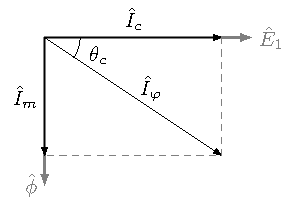
\includegraphics{figTransformersCoreLossAndMagnetizingCurrents}
\caption{مختلف مرحلی سمتیوں کے زاویے۔}
\label{شکل_ٹرانسفارمر_مرکزی_ضیاع_اور_مقناطیسی_رو}
\end{figure}

غیر سائن نما ہیجان انگیز برقی رو \عددیء{\i_{\varphi}} کو \اصطلاح{فوریئر} تسلسل\فرہنگ{فوریئر تسلسل}\حاشیہب{Fourier series}\فرہنگ{Fourier series} سے یوں لکھ سکتے ہیں۔
\begin{align} 
i_{\varphi}=\sum_n {\left( a_n \cos n \omega t + b_n \sin \omega t \right)}
\end{align}
اس میں \عددیء{(a_1 \cos \omega t+b_1 \sin \omega t)} کو \اصطلاح{بنیادی جزو}\فرہنگ{بنیادی جزو}\حاشیہب{fundamental component}\فرہنگ{fundamental component} کہتے ہیں اور باقی حصہ کو  \اصطلاح{موسیقائی جزو}\فرہنگ{موسیقائی جزو}\حاشیہب{harmonic components}\فرہنگ{harmonic components}  کہتے ہیں۔ بنیادی جزو میں \عددیء{a_1 \cos \omega t}، مقناطیسی بہاو سے وجود میں آنے والے امالی برقی دباو \عددیء{e_1} ،  جو کہ مساوات \حوالہ{مساوات_ٹڑانسفارمر_دباو_سمتیہ} میں دی گئی ہے کے ہم قدم ہے۔ یعنی  یہ دونوں وقت کے ساتھ یکساں بڑھتے اور گھٹتے ہیں جبکہ اس میں \عددیء{b_1 \sin \omega t} نوے درجہ زاویہ \عددیء{e_1}  کے پیچھے رہتا ہے۔ قالب میں مختلف وجوہات سے برقی طاقت کی ضائع  کو \عددیء{a_1 \cos \omega t} ظاہر  کرتی ہے۔اسی لئے اس جزو کو \اصطلاح{جزو قالبی ضیاع}\فرہنگ{قالبی ضیاع!جزو}\حاشیہب{core loss component}\فرہنگ{core loss component}  کہتے ہیں۔ہیجان انگیز برقی رو \عددیء{i_{\varphi}} سے اگر \عددیء{a_1 \cos \omega t} منفی کی جائے تو بقایا کو مقناطیس بنانے والا برقی رو\فرہنگ{مقناطیسی برقی رو} یا \اصطلاح{مقناطیسی برقی رو}\حاشیہب{magnetizing current}\فرہنگ{magnetizing current} کہتے ہیں۔ اس  کی تیسری موسیقائی جزو سب سے زیادہ اہم  ہے۔ قوی  ٹرانسفارمروں میں یہ تیسری موسیقائی جزو عموماً  کُل ہیجان انگیز برقی رو  کے \عددیء{40} فی صد ہوتی ہے۔  

سوائے وہاں، جہاں  ہیجان انگیز برقی رو کے اثرات پر غور کیا جا رہا ہو، ہم ہیجان انگیز برقی رو کے غیر سائن نما ہونے کو نظرانداز کرتے ہیں۔ قوی ٹرانسفارمر کی  ہیجان انگیز برقی رو اس کی کُل برقی رو\حاشیہد{کُل برقی رو سے مراد وہ برقی رو ہے جو کُل برقی بوجھ لادنے سے حاصل ہو} کے صرف \عددیء{5}  فی صد کے قریب ہوتی ہے۔ لہٰذا  اس کا اثر بہت کم ہوتا ہے۔ لہٰذا ہم  ہیجان انگیز برقی رو کو سائن نما تصور کر کے اس کے اثرات پر غور کرتے ہیں۔ایسا کرنے سے مسئلہ پر غور کرنا آسان ہو جاتا ہے۔ اس فرضی سائن نما  ہیجان انگیز برقی رو\حاشیہد{یعنی  بدلتی برقی رو \عددیء{i_{\varphi}} کو اب مرحلی سمتیہ کی مدد سے \عددیء{\hat{I_{\varphi}}} لکھتے ہیں} \عددیء{\hat{I_{\varphi}}}  کی موثر قیمت \عددیء{I_{\varphi,rms}} ، اصل  ہیجان انگیز برقی رو کی موثر قیمت کے برابر رکھی جاتی ہے جبکہ اس کا زاویہ \عددیء{\theta_c} یوں رکھا جاتا ہے کہ اس سے حاصل برقی ضیاع اصل برقی ضیاع کے برابر ہو۔ شکل \حوالہ{شکل_ٹرانسفارمر_مرکزی_ضیاع_اور_مقناطیسی_رو}  کی مدد سے یہ بات سمجھنی زیادہ آسان ہے۔ شکل میں اگر دیکھا جائے تو
\begin{align}
p_c=E_{rms} I_{\varphi,rms} \cos \theta_c
\end{align}
جہاں \عددیء{p_c} \اصطلاح{قالبی ضیاع}  ہے۔ لہٰذا  اگر \عددیء{\hat{I_{\varphi}}} اور \عددیء{\hat{E_1}} کے مابین \عددیء{\theta_c} کا زاویہ ہو تو اس سے قالبی ضیاع صحیح حاصل ہوتا ہے۔\عددیء{\hat{I_{\varphi}}} اسی زاویہ  سے  \عددیء{\hat{E_1}}  کے پیچھے رہتا ہے۔

\حصہ{تبادلہ برقی دباو اور تبادلہ برقی رو کے خصوصیات}
ہم شکل \حوالہ{شکل_ٹرانسفارمر_کامل_بار_بردار_ٹرانسفارمر}  کی مدد سے ٹرانسفارمر کا مطالعہ کرتے ہیں۔  ہم فرض کرتے ہیں کہ ابتدائی جانب لچھے کے \عددیء{N_1} اور ثانوی جانب لچھے کے \عددیء{N_2} چکر ہیں اور یہ کہ ان  دونوں لچھوں کی مزاحمت صفر ہے۔ ہم مزید یہ کہتے ہیں کہ پوری مقناطیسی بہاو  قالب ہی میں رہتا ہے اور دونوں لچھوں سے گزرتا ہے۔ قالب میں برقی توانائی ضائع نہیں ہوتی اور اس کی مقناطیسی مستقل اتنی زیادہ ہے کہ ہیجان انگیز برقی رو قابلِ نظر انداز ہے۔ برقی رو \عددیء{i_1}  اور \عددیء{i_2} کی سمتیں یوں رکھی گئی ہیں کہ ان سے وجود میں آنے والے مقناطیسی بہاو ایک دوسرے کی اُلٹ سمتوں میں  ہیں۔ اصل ٹرانسفارمر ان باتوں پر تقریباً پورے اترتے ہیں۔ ایسے ٹرانسفارمر کو کامل ٹرانسفارمر\فرہنگ{ٹرانسفارمر!کامل}\حاشیہب{ideal transformer}\فرہنگ{transformer!ideal}  کہتے ہیں۔
\begin{figure}
\centering
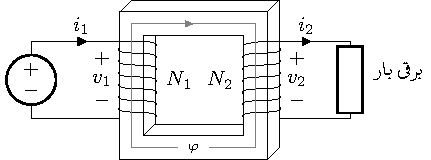
\includegraphics{figTransformersLoadedIdealTransformer}
\caption{کامل بوجھ بردار ٹرانسفارمر۔}
\label{شکل_ٹرانسفارمر_کامل_بار_بردار_ٹرانسفارمر}
\end{figure}

جب اس کامل ٹرانسفارمر کے ابتدائی لچھے پر بدلتی برقی دباو \عددیء{v_1} لاگو کیا جائے تو اس کے قالب میں بدلتا مقناطیسی بہاو  \عددیء{\varphi_m} وجود میں  آئے گا جو ابتدائی لچھے میں   لاگو برقی دباو \عددیء{v_1} کے برابر امالی برقی دباو \عددیء{e_1} کو جنم دے گا۔لہٰذا
\begin{align}
v_1=e_1=N_1 \frac{\dif \varphi_m}{\dif t}
\end{align}
یہ مقناطیسی بہاو دوسرے لچھے سے بھی گزرے گا اور اس میں \عددیء{e_2} امالی برقی دباو کو جنم دے گا جو ثانوی جانب کے سروں پر برقی دباو \عددیء{v_2}  کی صورت میں حاصل ہو گا۔ یعنی
\begin{align}
v_2=e_2=N_2 \frac{\dif \varphi_m}{\dif t}
\end{align}
ان دونوں کی نسبت سے
\begin{align}\label{مساوات_ٹرانسفارمر_تبادلہ_دباو}
\frac{v_1}{v_2}=\frac{N_1 \frac{\dif \varphi_m}{\dif t}}{N_2 \frac{\dif \varphi_m}{\dif t}}=\frac{N_1}{N_2}
\end{align}
لہٰذا ایک کامل ٹرانسفارمر دونوں لچھوں کے چکروں کی نسبت سے \اصطلاح{تبادلہ برقی دباو}\فرہنگ{برقی دباو!تبادلہ}\حاشیہب{voltage transformation}\فرہنگ{voltage!transformation} کرتا ہے۔

چونکہ یہ ایک کامل ٹرانسفارمر ہے لہٰذا اسے جتنی برقی طاقت ابتدائی جانب  دی جائے اتنی ہی برقی طاقت اس سے ثانوی جانب حاصل ہو گی،یعنی
\begin{align}
p=v_1 i_1 = v_2 i_2
\end{align}
یا
\begin{align}
\frac{v_1}{v_2}=\frac{i_2}{i_1}
\end{align}
مساوات  \حوالہ{مساوات_ٹرانسفارمر_تبادلہ_دباو} کی مدد سے
\begin{align}
\frac{v_1}{v_2}=\frac{i_2}{i_1}=\frac{N_1}{N_2}
\end{align}
یہ ایک انتہائی اہم نتیجہ ہے جو ٹرانسفارمر کی تبادلہ برقی دباو اور \اصطلاح{تبادلہ برقی رو}\فرہنگ{برقی رو!تبادلہ}\حاشیہب{current transformation}\فرہنگ{current!transformation}  کی خصوصیات بیان کرتا ہے۔اسے عموماً دو حصوں میں یوں لکھا جاتا ہے۔
\begin{gather}
\begin{aligned}\label{مساوات_ٹرانسفارمر_تبادلہ_دباو_رو}
\frac{v_1}{v_2}&=\frac{N_1}{N_2}\\
\frac{i_1}{i_2}&=\frac{N_2}{N_1}
\end{aligned}
\end{gather}
اس مساوات کی پہلی جزو کہتی ہے کہ ٹرانسفارمر کی دونوں جانب برقی دباو  ان کے چکروں کی راست متناسب  ہو گا جبکہ مساوات کی دوسری جزو کہتی ہے کہ ٹرانسفارمر کے دونوں جانب برقی رو ان کے چکروں کے بالعکس متناسب ہو گا۔

\ابتدا{مثال}
	شکل  \حوالہ{شکل_ٹرانسفارمر_کامل_بار_بردار_ٹرانسفارمر}  میں اگر
\begin{align*}
\hat{V_1}&=220 \phase{0}\\
N_1:N_2&=220:22\\
Z&=R=\SI{10}{\ohm}
\end{align*}
ہوں تو ٹرانسفارمر کی دونوں جانب برقی دباو اور برقی رو معلوم کریں۔

حل:
ابتدائی جانب برقی دباو دیا گیا ہے یعنی \عددیء{220} وولٹ جبکہ ثانوی جانب برقی دباو مساوات \حوالہ{مساوات_ٹرانسفارمر_تبادلہ_دباو_رو} کی پہلی جزو کی مدد سے حاصل کیا جاتا ہے یعنی
\begin{align*}
\hat{V_2}=\frac{N_2}{N_1} \hat{V_1}=\frac{22}{220} \times 220\phase {0}=22\phase{0}
\end{align*}
ثانوی جانب \عددیء{22} وولٹ ہیں جو ابتدائی جانب برقی دباو کے ہم قدم ہے۔ثانوی جانب یہ برقی دباو \عددیء{10} اوہم کی مزاحمت میں برقی رو پیدا کرے گا جسے اوہم کے قانون سے حاصل کیا جاتا ہے یعنی
\begin{align*}
\hat{I_2}=\frac{22 \phase {0}}{10}=2.2\phase {0}
\end{align*}
ثانوی جانب \عددیء{2.2} ایمپیئر برقی رو ہے۔ ابتدائی جانب کی برقی رو مساوات \حوالہ{مساوات_ٹرانسفارمر_تبادلہ_دباو_رو} کی دوسری جزو کی مدد سے حاصل کی جاتی ہے یعنی
\begin{align*}
\hat{I_1}=\frac{N_2}{N_1} \hat{I_2}=\frac{22}{220} \times 2.2\phase{0}=0.22\phase{0}
\end{align*}
\انتہا{مثال}

اس مثال کے نتائج ایک جگہ لکھ کر ان پر غور کرتے ہیں۔
\begin{align*}
\hat{V_1}=220\phase{0}, \quad \hat{V_2}=22\phase{0}, \quad \hat{I_1}=0.22\phase{0}, \quad \hat{I_2}=2.2\phase{0}
\end{align*}
ہم دیکھتے ہیں ابتدائی جانب برقی دباو ثانوی جانب کی برقی دباو کے دس گنا ہے جبکہ برقی رو میں قصہ اُلٹ ہے۔ثانوی جانب کی برقی رو ابتدائی جانب کی برقی رو کے دس گنا ہے۔طاقت دونوں جانب برابر ہے۔یہ نہایت اہم ہے کہ آپ اس بات کو اچھی طرح سمجھ لیں کہ جس جانب برقی دباو زیادہ ہوتا ہے اس جانب برقی رو کم ہوتی ہے۔ لہٰذا زیادہ برقی دباو کی جانب لچھے کے چکر زیادہ ہوں گے اور اس لچھے میں نسبتاً باریک برقی تار استعمال ہو گی جبکہ کم برقی دباو کا لچھا کم چکر کا ہو گا اور اس میں نسبتاً موٹی برقی تار استعمال ہو گی۔ 

\ابتدا{مثال}
	صفحہ \حوالہصفحہ{شکل_ٹرانسفارمر_رکاوٹ_کا_تبادلہ} پر دکھائے گئے شکل \حوالہ{شکل_ٹرانسفارمر_رکاوٹ_کا_تبادلہ}-الف سے رجوع کریں۔ اس شکل میں رکاوٹ \عددیء{Z_2} کو  بدلتی برقی دباو \عددیء{\hat{V_1}} کے ساتھ ایک ٹرانسفارمر کے ذریعہ جوڑا گیا ہے۔اگر
\begin{align*}
\hat{V_1}=110\phase{0},\quad Z_2=R+j X=3+j 2,\quad N_1:N_2=220:22 
\end{align*}
ہوں تو رکاوٹ میں برقی رو اور طاقت کا ضیاع معلوم کریں۔

حل:
	ٹرانسفارمر کی تبادلہ برقی دباو کی خصوصیت سے اس کے ابتدائی جانب \عددیء{110} وولٹ برقی دباو ٹرانسفارمر کی ثانوی جانب تبدیل ہو کر  \عددیء{\hat{V_s}} ہو جائیں گے جہاں
\begin{align*}
\hat{V_s}=\frac{N_2}{N_1} \hat{V_1}=\frac{22}{220} \times 110\phase{0}=11\phase{0}
\end{align*}
ہے لہٰذا
\begin{align*}
\hat{I_2}=\frac{\hat{V_s}}{Z}=\frac{11\phase{0}}{3+j 2}= 3.05\phase{-33.69\degree}
\end{align*}
اور برقی طاقت کا ضیاع \عددیء{p_z}
\begin{align*}
p_z=I_2^2 R=3.05^2 \times 3=\SI{27.9}{\watt}
\end{align*}
\انتہا{مثال}

\حصہ{ثانوی جانب بوجھ کا ابتدائی جانب اثر}\شناخت{حصہ_ٹرانسفارمر_ثانوی_بار_کا_ابتدائی_جانب_اثر}
یہاں صفحہ \حوالہصفحہ{شکل_ٹرانسفارمر_کامل_بار_بردار_ٹرانسفارمر} پر دکھائے گئے  شکل \حوالہ{شکل_ٹرانسفارمر_کامل_بار_بردار_ٹرانسفارمر}  سے رجوع کریں۔ہم حصہ \حوالہ{حصہ_ٹرانسفارمر_امالی_برقی_دباو}  میں دیکھ چکے ہیں کہ اگر ایک بے بوجھ ٹرانسفارمر کی ابتدائی لچھے پر بدلتی برقی دباو \عددیء{v_1} لاگو کی جائے تو اس لچھے میں ہیجان انگیز برقی رو \عددیء{i_{\varphi}} گزرے گی۔اس برقی رو کی مقناطیسی دباو \عددیء{N_1 i_{\varphi}} قالب میں مقناطیسی بہاو \عددیء{\varphi_m}\حاشیہد{\عددیء{\varphi} کو یہاں \عددیء{\varphi_m} کہا گیا ہے۔} کو جنم دے گی ۔اگر لچھے کی مزاحمت صفر ہو تو \عددیء{\varphi_m} ابتدائی لچھے میں \عددیء{e_1} امالی برقی دباو پیدا کرے گی جہاں
\begin{align}\label{مساوات_ٹرانسفارمر_دباو_برابر_بہاو_تفرق}
v_1=e_1=N_1 \frac{\dif \varphi_m}{\dif t}
\end{align}
ہو گی۔

اب ہم ثانوی جانب  برقی بوجھ لادتے ہیں۔ ایسا کرنے سے بوجھ بردار ٹرانسفارمر\فرہنگ{ٹرانسفارمر!بوجھ بردار}\حاشیہب{loaded transformer}  کے  ثانوی جانب  برقی رو \عددیء{i_2} رواں ہو گی جس کی وجہ سے \عددیء{N_2 i_2} مقناطیسی دباو وجود میں آئے گی۔ اس مقناطیسی دباو کی وجہ سے قالب میں مقناطیسی بہاو \عددیء{\varphi_{\textup{بوجھ}}}  پیدا ہو گا۔ اگر اس مقناطیسی بہاو کا کچھ  نہ کیا جائے تو قالب میں پہلے سے موجود مقناطیسی بہاو تبدیل ہو کر \عددیء{\varphi_{\textup{نئی}}=\varphi_{m}-\varphi_{\textup{بوجھ}}} ہو جائے گا اور یوں ابتدائی لچھے میں امالی دباو تبدیل ہو کر \عددیء{e_{\textup{نئی}}} ہو جائے گا۔  لہٰذا ابتدائی جانب پر اب امالی دباو اور اس پر لاگو برقی دباو برابر نہیں ہونگے جو کہ مساوات \حوالہ{مساوات_ٹرانسفارمر_دباو_برابر_بہاو_تفرق}  کی موجودگی میں ناممکن ہے۔ لہٰذا اس مقناطیسی بہاو \عددیء{\varphi_{\textup{بوجھ}}}  کے اثر کو ختم کرنے کیلئے ابتدائی لچھے میں برقی رو \عددیء{i_{1}} نمودار ہو گی جو اس مقناطیسی دباو یعنی \عددیء{N_2 i_2} کے اثر کو ختم کر دے گی یعنی
\begin{align}
N_1 i_1=N_2 i_2
\end{align}
یہ وہ ذریعہ ہے جس سے ابتدائی جانب معلوم ہوتا ہے کہ ثانوی جانب پر بوجھ لدا ہے۔ شکل میں دونوں لچھوں میں برقی رو کی سمتیں یوں ہیں کہ ان کے مقناطیسی بہاو آپس میں اُلٹ سمت میں ہیں لہٰذا  قالب میں اب پھر مقناطیسی بہاو \عددیء{\varphi_m}  کے برابر  ہے جیسا کہ ہونا چاہئے تھا۔ اس مساوات کو یوں لکھ سکتے ہیں
\begin{align}\label{مساوات_ٹرانسفارمر_برقی_رو_اور_چکر_شرح}
\frac{i_1}{i_2}=\frac{N_2}{N_1}
\end{align}
یہ وہی مساوات ہے جو کامل ٹرانسفارمر کے لئے ثابت کی گئی تھی۔
%
\حصہ{ٹرانسفارمر کی علامت پر نقطوں کا مطلب}
	شکل \حوالہ{شکل_ٹرانسفارمر_کامل_بار_بردار_ٹرانسفارمر}  میں ٹرانسفارمر کے لچھوں پر نکتے لگائے گئے ہیں۔ یہ نکتے اس بات کو ظاہر کرتے ہیں کہ اگر ایک طرف کے لچھے پر برقی دباو \عددیء{v_1} یوں ہو کہ نکتے والا سرا مثبت اور بغیر نکتے والا سرا منفی ہو تو دوسرے لچھے  پر برقی دباو \عددیء{v_2} اس طرح ہو گا کہ اس لچھے کا بھی  نکتے والا سرا مثبت اور بغیر نکتے والا سرا منفی ہو گا۔

مزید یہ کہ ابتدائی جانب برقی رو ٹرانسفارمر کے نکتے والے سرے سے ٹرانسفارمر کی اندر جانب ہو گا جبکہ ثانوی جانب برقی رو نقطہ والے سرے سے ٹرانسفارمر سے باہر نکلے گا۔

 یوں  \عددیء{v_1} اور \عددیء{v_2} وقت کے ساتھ یکساں تبدیل ہوتے ہیں اور ان کے مابین صفر زاویہ ہے۔ لہٰذا یہ دو برقی دباو \اصطلاح{ہم قدم}\فرہنگ{ہم قدم}\حاشیہب{in-phase}\فرہنگ{in-phase} ہیں۔

\حصہ{رکاوٹ کا تبادلہ}
اس حصہ میں کامل ٹرانسفارمر میں رکاوٹ کے تبادلہ پر غور کیا جائے گا۔شکل \حوالہ{شکل_ٹرانسفارمر_رکاوٹ_کا_تبادلہ}-الف میں ایک ٹرانسفارمر دکھایا گیا ہے جس کی ابتدائی جانب سائن نما برقی دباو  \عددیء{\hat{V_1}=V_1\phase{\theta}}  لاگو کیا گیا ہے۔یہاں مرحلی سمتیہ استعمال کئے جائیں گے۔

جیسے اُوپر ذِکر ہوا، برقی دباو \عددیء{\hat{V_1}} اور \عددیء{\hat{V_2}} آپس میں ہم قدم ہیں اور  اسی طرح برقی رو \عددیء{\hat{I_1}} اور \عددیء{\hat{I_2}} آپس میں  ہم قدم ہیں۔مساوات \حوالہ{مساوات_ٹرانسفارمر_تبادلہ_دباو} اور  مساوات \حوالہ{مساوات_ٹرانسفارمر_برقی_رو_اور_چکر_شرح}   کو مرحلی سمتیہ کی مدد سے یوں لکھ سکتے ہیں
\begin{gather}
\begin{aligned}
\hat{V_1}&=\left(\frac{N_1}{N_2} \right) \hat{V_2}\\
\hat{I_1}&=\left(\frac{N_2}{N_1} \right) \hat{I_2}
\end{aligned}
\end{gather}
چونکہ رکاوٹ
\begin{align}
Z_2=\frac{\hat{V_2}}{\hat{I_2}}=\abs{Z_2}\phase{\theta_z}
\end{align}
کے برابر ہے لہٰذا
\begin{align}\label{مساوات_ٹرانسفارمر_تبادلہ_رکاوٹ_الف}
\frac{\hat{V_1}}{\hat{I_1}}=\left(\frac{N_1}{N_2} \right)^2 \frac{\hat{V_2}}{\hat{I_2}}=\left(\frac{N_1}{N_2} \right)^2  Z_2
\end{align}
اب اگر ہم ٹرانسفارمر بمع اس پر لدے رکاوٹ  کی جگہ برقی دباو \عددیء{\hat{V_1}} کو رکاوٹ \عددیء{Z_1} پر لاگو کریں جہاں اس رکاوٹ کی قیمت
\begin{align}\label{مساوات_ٹرانسفارمر_متبادل_رکاوٹ_تعریف}
Z_1=\left(\frac{N_1}{N_2} \right)^2  Z_2
\end{align}
ہو تو \عددیء{\hat{V_1}} سے حاصل برقی رو یا اس سے حاصل برقی طاقت تبدیل نہیں ہو گی۔یہ شکل \حوالہ{شکل_ٹرانسفارمر_رکاوٹ_کا_تبادلہ}-ب میں دکھایا گیا ہے جہاں سے واضح ہے کہ
\begin{align}\label{مساوات_ٹرانسفارمر_تبادلہ_رکاوٹ_ب}
\frac{\hat{V_1}}{\hat{I_1}}=Z_1=\left(\frac{N_1}{N_2} \right)^2  Z_2
\end{align}
لہٰذا شکل کے الف اور ب دونوں حصوں سے  برقی دباو \عددیء{\hat{V_1}} کی برقی رو مساوات \حوالہ{مساوات_ٹرانسفارمر_تبادلہ_رکاوٹ_الف}  اور مساوات \حوالہ{مساوات_ٹرانسفارمر_تبادلہ_رکاوٹ_ب}  سے یکساں حاصل ہوتی ہے یعنی
\begin{align}
\hat{I_1}=\frac{\hat{V_1}}{\left(\frac{N_1}{N_2} \right)^2  Z_2}
\end{align}
اور یوں الف اور با  دونوں حصوں میں  برقی دباو \عددیء{\hat{V_1}} سے حاصل برقی طاقت برابر ہے یعنی
\begin{align}
p=\hat{V_1} \cdot \hat{I_1}=\frac{V_1^2 \cos \theta_z}{\left(\frac{N_1}{N_2} \right)^2  \abs{Z_2}}
\end{align}
%
\begin{figure}
\centering
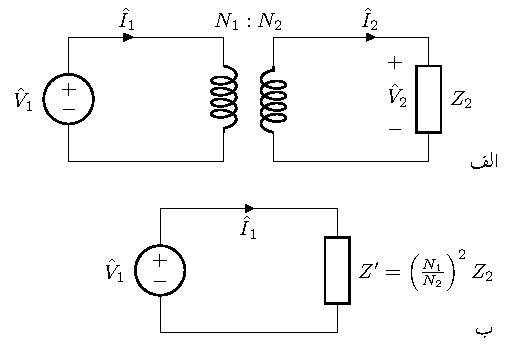
\includegraphics{figTransformersImpedanceTransformation}
\caption{ٹرانسفارمر کی تبادلہ رکاوٹ کی خصوصیت۔}
\label{شکل_ٹرانسفارمر_رکاوٹ_کا_تبادلہ}
\end{figure}
	یوں اگر ٹرانسفارمر کے ثانوی جانب  رکاوٹ \عددیء{Z_2} کا بوجھ ہو تو حساب کرتے وقت ہم یہ اخذ کر سکتے ہیں کہ  ٹرانسفارمر بمع رکاوٹ \عددیء{Z_2} کی  جگہ  صرف  \عددیء{Z_1} رکاوٹ لگی ہے، جہاں \عددیء{Z_1} مساوات \حوالہ{مساوات_ٹرانسفارمر_متبادل_رکاوٹ_تعریف}  سے حاصل ہوتی ہے۔ رکاوٹ کا یوں ٹرانسفارمر کی ایک جانب سے دوسری جانب تبادلہ کیا جاسکتا ہے۔ٹرانسفارمر کی اس خاصیت کو  \اصطلاح{تبادلہ رکاوٹ}\فرہنگ{تبادلہ!رکاوٹ}\حاشیہب{impedance transformation}\فرہنگ{impedance transformation} کی خصوصیت  کہتے ہیں۔
%
\ابتدا{مثال}
شکل \حوالہ{شکل_ٹرانسفارمر_برقی_طاقت_کی_منتقلی}-الف میں رکاوٹ \عددیء{Z_B} کا برقی بوجھ ایک جنریٹر پر لدا ہے۔بوجھ تک برقی طاقت دو برقی تاروں کے ذریعہ منتقل کیا گیا ہے۔ان تاروں کی مجموعہ رکاوٹ \عددیء{Z_t} ہے۔
\begin{figure}
\centering
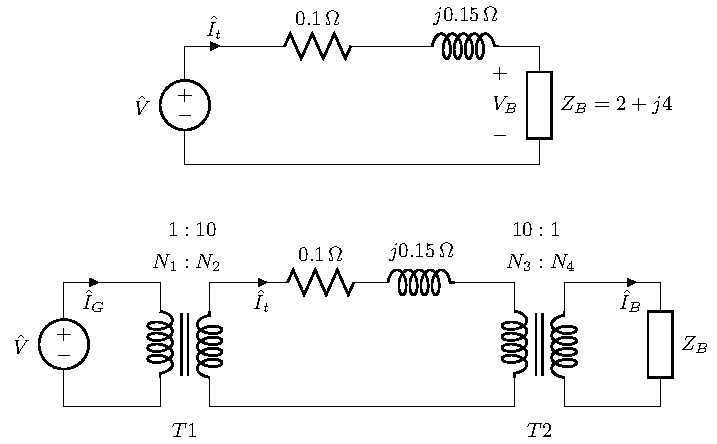
\includegraphics{figTransformersPowerTransmission}
\caption{برقی طاقت کی منتقلی۔}
\label{شکل_ٹرانسفارمر_برقی_طاقت_کی_منتقلی}
\end{figure}
%
\begin{figure}
\centering
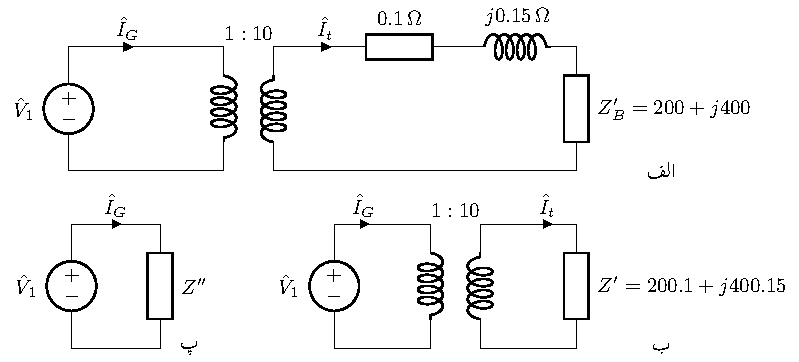
\includegraphics{figTransformersStepByStepSolution}
\caption{ٹرانسفارمر قدم با قدم حل کرنے کا طریقہ۔}
\label{شکل_ٹرانسفارمر_قدم_با_قدم_حل}
\end{figure}

شکل-ب میں جنریٹر کے قریب نسب برقی دباو بڑھانے والا ٹرانسفارمر برقی دباو کو دس گنا بڑھاتا ہے اور برقی بوجھ کے قریب نسب برقی دباو گھٹانے والا ٹرانسفارمر برقی دباو کو دس گنا گھٹاتا ہے۔اس حصہ میں وہی برقی تار استعمال کئے گئے ہیں لہٰذا ان کی بھی مجموعہ رکاوٹ \عددیء{Z_t} ہی ہے۔
اگر 
\begin{align*}
Z_B=2+j 4, \quad Z_t=0.1 +j 0.15, \quad \hat{V}=415\phase{0}
\end{align*}
ہوں تو دونوں صورتوں میں
\begin{itemize}
\item
برقی بوجھ پر برقی دباو معلوم کریں،
\item
برقی تاروں میں برقی طاقت کی ضیاع معلوم کرین۔
\end{itemize}

حل الف:
\begin{align*}
\hat{I_G}=\hat{I_t}=\hat{I_B}&=\frac{\hat{V}}{Z_t+Z_B}=\frac{415\phase{0}}{0.1+j 0.15+2+j 4}\\
&=\frac{415\phase{0}}{2.1+j 4.15}=89.23\phase{-63.159\degree}\\
&=40.3-j79.6
\end{align*}
یوں رکاوٹ پر برقی دباو
\begin{align*}
\hat{V_B}=\hat{I_B} Z_B&=\left(40.3-j79.6 \right) \left( 2+j 4\right)\\
&=399+j2=399\phase{0.287\degree}
\end{align*}
اور برقی تاروں میں برقی طاقت کا ضیاع ہے
\begin{align*}
p_t=I_t^2 R_t=89.23^2 \times 0.1=\SI{796}{\watt}
\end{align*}

حل ب:
شکل \حوالہ{شکل_ٹرانسفارمر_برقی_طاقت_کی_منتقلی} اور شکل \حوالہ{شکل_ٹرانسفارمر_قدم_با_قدم_حل}  سے رجوع کریں۔شکل  \حوالہ{شکل_ٹرانسفارمر_برقی_طاقت_کی_منتقلی} میں ٹرانسفارمر \عددیء{T_2} کے ثانوی جانب رکاوٹ کا مساوات \حوالہ{مساوات_ٹرانسفارمر_متبادل_رکاوٹ_تعریف}  کی مدد سے اس کی ابتدائی جانب تبادلہ سے ملتا ہے
\begin{align*}
Z_B'=Z_1=\left(\frac{N_3}{N_4} \right)^2 Z_B=\left(\frac{10}{1} \right)^2 \left(2+j 4 \right)=200+j 400
\end{align*}
یوں شکل \حوالہ{شکل_ٹرانسفارمر_قدم_با_قدم_حل}-الف حاصل ہوتا ہے۔اس شکل میں اب برقی تار کی رکاوٹ اور  تبادلہ شدہ رکاوٹ سلسلہ وار جُڑے ہیں۔ان کے مجموعہ  کو \عددیء{Z'} کہتے ہوئے
\begin{align*}
Z'=Z_t+Z_B'=0.1+j 0.15+200+j 400=200.1+j400.15
\end{align*}
یہ شکل \حوالہ{شکل_ٹرانسفارمر_قدم_با_قدم_حل}-ب میں دکھایا گیا ہے۔ایک مرتبہ دوبارہ مساوات \حوالہ{مساوات_ٹرانسفارمر_متبادل_رکاوٹ_تعریف}  استعمال کرتے ہوئے
\begin{align*}
Z''=\left(\frac{N_1}{N_2} \right)^2 Z'=\left(\frac{1}{10} \right)^2 \left(200.1+j400.15 \right)=2.001+j4.0015
\end{align*}
شکل \حوالہ{شکل_ٹرانسفارمر_قدم_با_قدم_حل}-پ میں دکھایا گیا ہے۔اب
\begin{align*}
\hat{I_G}=\frac{\hat{V}}{Z''}=\frac{415\phase{0}}{2.001+j4.0015}=92.76\phase{-63.432\degree}
\end{align*}
یہاں سے شکل \حوالہ{شکل_ٹرانسفارمر_قدم_با_قدم_حل}-ب  کی مدد سے اگر جنریٹر کی برقی رو معلوم ہو تو تبادلہ برقی رو سے
\begin{align*}
\hat{I_t}=\left(\frac{N_1}{N_2} \right) \hat{I_G}=\left(\frac{1}{10}\right) 92.76\phase{-63.432\degree}=9.276\phase{-63.432\degree}
\end{align*}
اس سے برقی تار میں طاقت کا ضیاع
\begin{align*}
p_t=I_t^2 R_t=9.276^2  \times 0.1=\SI{8.6}{\watt}
\end{align*}
اسی طرح شکل \حوالہ{شکل_ٹرانسفارمر_برقی_طاقت_کی_منتقلی}  میں اگر \عددیء{\hat{I_t}} معلوم ہو تو تبادلہ برقی رو سے
\begin{align*}
\hat{I_B}&=\left(\frac{N_3}{N_4}\right) \hat{I_t}=\left(\frac{10}{1}\right) 9.276\phase{-63.432\degree}\\
&=92.76\phase{-63.432\degree}=41.5-j 82.9
\end{align*}
اور رکاوٹ پر برقی دباو
\begin{align*}
\hat{V_B}=\hat{I_B} Z_B=\left(41.5-j 82.9 \right) \left(2+j 4 \right)=414+j 0.2
\end{align*}
ہو گی۔

ٹرانسفارمر کے بغیر برقی طاقت کی منتقلی میں برقی تاروں میں طاقت کی ضیاع \عددیء{796} واٹ ہے جبکہ ٹرانسفارمر کے استعمال سے یہ صرف \عددیء{8.6} واٹ ہے یعنی \عددیء{92} گنا کم۔یہی ٹرانسفارمر کی نہایت مقبولیت کی وجہ ہے۔ 
\انتہا{مثال}
%
\حصہ{ٹرانسفارمر کے وولٹ-ایمپیئر}
ٹرانسفارمر کی دونوں جانب برقی دباو ان لچھوں کے چکر پر منحصر ہوتا ہے۔ٹرانسفارمر ایک خاص برقی دباو اور برقی رو کے لئے بنائے جاتے ہیں۔ٹرانسفارمر جس برقی دباو \عددیء{V_1:V_2} کے لئے بنائے جائیں یہ اس سے کم برقی دباو پر بھی استعمال کئے جا سکتے ہیں اگرچہ یہ عموماً بنائے گئے برقی دباو پر ہی چلائے جاتے ہیں۔اسی طرح ٹرانسفارمر جتنی برقی رو \عددیء{I_1:I_2} کے لئے بنائے جائیں انہیں اس سے کم برقی رو پر استعمال کیا جا سکتا ہے۔حقیقت میں عموماً ٹرانسفارمر سے حاصل برقی رو اس حد سے کم ہی رکھی جاتی ہے۔

ٹرانسفارمر کی ایک جانب کی برقی دباو اور برقی رو کا حاصل ضرب اس کی دوسری جانب کی برقی دباو اور برقی رو کے حاصل ضرب کے برابر ہوتا ہے یعنی
\begin{align}
V_1 I_1=V_2 I_2
\end{align}
برقی دباو اور برقی رو کے حاصلِ ضرب  یعنی \عددیء{V_1 I_1} یا \عددیء{V_2 I_2} کو ٹرانسفارمر کی وولٹ ضربِ ایمپیئر کہتے ہیں جسے عموماً چھوٹا کر کے صرف \اصطلاح{وولٹ-ایمپیئر}\فرہنگ{وولٹ-ایمپیئر}
\حاشیہب{volt-ampere, VA}\فرہنگ{volt-ampere}\فرہنگ{VA}  کہا جاتا ہے\حاشیہد{وولٹ-ایمپیئر کو عموماً کلو وولٹ-ایمپیئر یعنی \عددیء{\si{\kilo \volt \ampere}} میں بیان کیا جاتا ہے}۔یہ ٹرانسفارمر کی برقی سکت کی ناپ ہے جو اس پر لگی تختی پر لکھا جاتا ہے۔اس تختی پر ٹرانسفارمر کے برقی دباو اور برقی تعداد ارتعاش بھی لکھے جاتے ہیں۔یوں ٹرانسفارمر کے وولٹ-ایمپیئر
\begin{align}\label{مساوات_ٹرانسفارمر_وولٹ_ایمپئیر}
\textup{وولٹ-ایمپیئر}= V_1 I_1 = V_2 I_2
\end{align}
ہوں گے۔

اگرچہ یہاں ذکر ٹرانسفارمر کا ہو رہا ہے دراصل برقی مشین یعنی موٹر اور جنریٹر کی تختیوں پر بھی ان کے چالو حالت کے برقی دباو، ان کے وولٹ-ایمپیئر اور برقی تعداد ارتعاش لکھے جاتے ہیں۔اس کی وجہ یہ ہے کہ ان سب مشین کی کارکردگی کے بنیادی اصول ایک ہی طرح کے ہیں۔

\ابتدا{مثال}
ایک \عددیء{25000 } وولٹ-ایمپیئر اور \عددیء{11000:220} وولٹ برقی سکت  کے ٹرانسفارمر کے زیادہ برقی دباو کی جانب \عددیء{11000} وولٹ لاگو ہیں۔
\begin{itemize}
\item
اس کی ثانوی جانب زیادہ سے زیادہ کتنی برقی بوجھ ڈالی جا سکتی ہے۔
\item
اس زیادہ سے زیادہ برقی بوجھ پر اس کے ابتدائی لچھے میں برقی رو حاصل کریں۔
\end{itemize}

حل:	اس ٹرانسفارمر کی معلومات یہ ہیں
\begin{align*}
\SI{25}{\kilo \volt \ampere}, \quad 11000:220\,\textup{V}
\end{align*}
اس کی ثانوی جانب برقی دباو تبادلہ برقی دباو کی مساوات سے  \عددیء{220 } وولٹ حاصل ہوتا ہے۔یوں اس کی ثانوی جانب یعنی کم برقی دباو کی جانب زیادہ سے زیادہ برقی رو مساوات \حوالہ{مساوات_ٹرانسفارمر_وولٹ_ایمپئیر}  سے حاصل کیا جاتا ہے۔
\begin{align*}
I_2=\frac{25000}{220}=\SI{113.636}{\ampere}
\end{align*}
اسی طرح اس کی ابتدائی جانب زیادہ سے زیادہ برقی رو اسی مساوات سے یوں حاصل ہوتی ہے
\begin{align*}
I_1=\frac{25000}{11000}=\SI{2.27}{\ampere}
\end{align*}
\انتہا{مثال}
%
ٹرانسفارمر کی دونوں جانب لچھوں میں استعمال برقی تار کی موٹائی یوں رکھی جاتی ہے کہ ان میں کثافتِ برقی رو \عددیء{J}\حاشیہد{\عددیء{\SI{1000}{\kilo \volt \ampere}}  ٹرانسفارمر کی لچھوں میں کثافتِ برقی رو تقریباً  \عددیء{\SI{3}{\ampere / \milli \meter \squared}} رکھی جاتی ہے} یکساں ہو۔لچھوں کی مزاحمت میں برقی رو گزرنے سے برقی طاقت کا ضیاع ہوتا ہے جس سے یہ گرم ہوتے ہیں۔ٹرانسفارمر کی برقی رو کی حد لچھوں کی گرمائش پر منحصر ہوتی ہے۔ان کی زیادہ سے زیادہ حرارت کو محفوظ حد کے اندر رکھا جاتا ہے۔

بڑے ٹرانسفارمر کے قالب اور لچھے ایک غیر موصل تیل سے بھری ٹینکی میں ڈبوئے رکھے جاتے ہیں۔یہ تیل ایک تو برقی لچھوں کی حرارت کم کرنے میں مدد دیتا ہے اور دوسری جانب غیر موصل ہونے کی وجہ سے یہ زیادہ برقی دباو کے حصوں کو برقی طور پر جدا رکھنے میں مدد دیتا ہے۔یہ تیل تقریباً  \عددیء{\SI{80}{\celsius}} پر خراب ہونا شروع ہو جاتا ہے اور ہر \عددیء{\SI{8}{\celsius}} اضافی درجہ حرارت پر اس کی زندگی آدھی ہوتی رہتی ہے۔یعنی اگر \عددیء{\SI{80}{\celsius}} پر تیل کی کارآمد زندگی \عددیء{x} سال ہے تو \عددیء{\SI{88}{\celsius}} پر \عددیء{x/2} سال اور  \عددیء{\SI{96}{\celsius}} پر یہ صرف  \عددیء{x/4} سال ہو گی۔

	ٹرانسفارمر جس برقی دباو کے لئے بنایا جائے  یہ اس پر لگی تختی پر لکھا جاتا ہے۔اس سے حاصل برقی رو کی حد کو ایک مختلف طریقے سے لکھا جاتا ہے۔

\حصہ{ٹرانسفارمر کے امالہ اور اس کے مساوی دور}
\جزوحصہ{لچھے کی مزاحمت اور اس کی متعاملہ علیحدہ کرنا}
ٹرانسفارمر کی ابتدائی لچھے کی مزاحمت \عددیء{R_1} کو ہم نے حصہ \حوالہ{حصہ_ٹرانسفارمر_امالی_برقی_دباو} مساوات \حوالہ{مساوات_ٹرانسفارمر_بیرونی_اندرونی_دباو_فرق} میں دیکھا۔لچھے کی مزاحمت کو لچھے سے باہر لچھے کے ساتھ سلسلہ وار جڑا دکھایا گیا تھا۔دیکھتے ہیں یہ کیسے ممکن ہوتا ہے۔

شکل \حوالہ{شکل_ٹرانسفارمر_لچھے_کی_مزاحمت_اور_متعاملہ}-الف میں ایک لچھے پر بدلتی برقی دباو لاگو کا گیا ہے۔اگر لچھے کی برقی تار کو نہایت چھوٹے ٹکڑوں میں تقسیم کیا جائے تو اس کے ہر ٹکڑے کی نہایت کم مزاحمت  اور متعاملہ ہو گی۔ایسا ایک ٹکڑا شکل-ب میں دکھایا گیا ہے۔چونکہ لچھا ان سب ٹکڑوں کے سلسلہ وار جڑنے سے بنا ہے  لہٰذا شکل-الف کو ہم شکل-پ کی طرح بنا سکتے ہیں جہاں لچھے کے \عددیء{n} ٹکڑے  کیے گیے ہیں۔
\begin{figure}
\centering
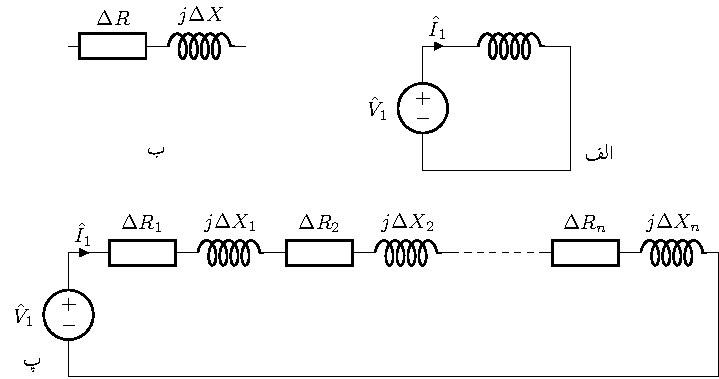
\includegraphics{figTransformersCoilResistanceAndReactance}
\caption{لچھے کی مزاحمت اور متعاملہ۔}
\label{شکل_ٹرانسفارمر_لچھے_کی_مزاحمت_اور_متعاملہ}
\end{figure}

اس دور کی مساوات لکھ کر حل کرتے ہیں۔
\begin{align*}
\hat{V}_1&=\hat{I}_1 \left(\Delta R_1 + j \Delta X_1 +\Delta R_2 + j \Delta X_2 + \cdots \Delta R_n + j \Delta X_n   \right)\\
&=\hat{I}_1 \left(\Delta R_1 +\Delta R_2 +\cdots \Delta R_n   \right)+\hat{I}_1 \left(j \Delta X_1 + j \Delta X_2+\cdots   j \Delta X_n   \right)\\
&=\hat{I}_1 \left( R +j X \right)
\end{align*}
جہاں
\begin{align*}
R&=\Delta R_1 +\Delta R_2 +\cdots \Delta R_n\\
X&=\Delta X_1 + \Delta X_2 +\cdots   \Delta X_n
\end{align*}
اس سے  شکل \حوالہ{شکل_ٹرانسفارمر_لچھے_کی_مزاحمت_اور_متعاملہ_کی_علیحدگی}  حاصل ہوتا ہے  جس سے  ثابت ہوتا ہے کہ حساب کتاب کی غرض سے لچھے کی مزاحمت اور متعاملہ علیحدہ کیے جا سکتے ہیں۔
\begin{figure}
\centering
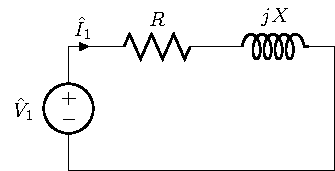
\includegraphics{figTransformersCoilResistanceAndReactanceSeparation}
\caption{لچھے کی مزاحمت اور متعاملہ کی علیحدگی۔}
\label{شکل_ٹرانسفارمر_لچھے_کی_مزاحمت_اور_متعاملہ_کی_علیحدگی}
\end{figure}
%
\جزوحصہ{رِستا امالہ}
اوپر ایک کامل ٹرانسفارمر زیرِ بحث رہا۔ اب ہم ٹرانسفارمر میں ان عناصر کا ذکر کرتے ہیں جن کی وجہ سے ٹرانسفارمر غیر کامل ہو جاتا ہے۔ بہت سی جگہوں پر ٹرانسفارمر استعمال کرتے وقت ان عناصر کو مدِ نظر رکھ کر ہی اس کا صحیح استعمال ممکن ہوتا ہے۔ ان عناصر کے اثر کو شامل کرنے کے لئے ہم  ٹرانسفارمر کا مساوی دور بناتے ہیں۔

ابتدائی لچھے کے مقناطیسی بہاو کو دو حصوں میں تقسیم کیا جا سکتا ہے۔ پہلا حصہ وہ جو قالب سے گزر کر ابتدائی اور ثانوی لچھے دونوں سے گزرتا ہے۔ یہ ان کا مشترکہ مقناطیسی بہاو ہے اور دوسرا حصہ وہ جو صرف ابتدائی لچھے سے گزرتا ہے اور زیادہ تر قالب کے باہر خلاء میں ہی رہتا ہے۔  اس کو \اصطلاح{رستا  مقناطیسی بہاو}\فرہنگ{مقناطیسی بہاو!رستا}\حاشیہب{leakage magnetic flux}\فرہنگ{magnetic flux!leakage}   کہتے ہیں۔ یہ شکل میں دکھایا گیا ہے۔ چونکہ ہوا میں مقناطیسی مستقل \عددیء{\mu_0} مقررہ ہے لہٰذا یہاں ہچکچاہٹ بھی مقررہ ہے۔  یوں رستا مقناطیسی بہاو ابتدائی لچھے کی برقی رو کے  براہ راست متناسب ہوتی ہے۔

 اس کے اثر کو بالکل لچھے کی مزاحمت کی طرح لچھے سے باہر \اصطلاح{رستا امالہ}\فرہنگ{رستا!امالہ}\حاشیہب{leakage inductance}\فرہنگ{leakage inductance} \عددیء{L_1} یا \اصطلاح{رستا متعاملہ}\فرہنگ{رستا!متعاملہ}\حاشیہب{leakage reactance}\فرہنگ{leakage reactance}  \عددیء{X_1=2\pi f L_1} سے ظاہر کیا جاتا ہے۔

ٹرانسفارمر کے ابتدائی لچھے میں برقی رو \عددیء{\hat{I_1}}  گزرنے سے رستا متعاملہ میں \عددیء{\hat{V}_{X1}=j \hat{I}_1 X_1} برقی دباو اور لچھے کے تار کی مزاحمت \عددیء{R_1} میں
 \عددیء{\hat{V}_{R1}=\hat{I}_1 R_1} برقی دباو گھٹتا ہے۔

یوں ابتدائی لچھے  پر لاگو برقی دباو \عددیء{\hat{V}_1} میں سے کچھ برقی دباو \عددیء{R_1} میں کم ہو گا،  کچھ  متعاملہ \عددیء{X_1} میں کم ہو گا اور بقایا  \عددیء{\hat{E}_1} کے برابر ہو گا۔  یہ شکل \حوالہ{شکل_ٹرانسفارمر_ماڈل_حصہ_اول}  میں دکھایا گیا ہے۔
\begin{figure}
\centering
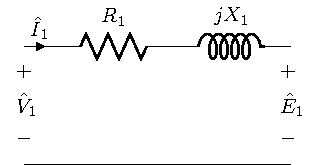
\includegraphics{figTransformersModelFirstPart}
\caption{ٹرانسفارمر مساوی دور، حصہ اول۔}
\label{شکل_ٹرانسفارمر_ماڈل_حصہ_اول}
\end{figure}
%

\جزوحصہ{ثانوی برقی رو اور قالب کے اثرات}
قالب میں دونوں لچھوں کا مشترکہ مقناطیسی بہاو ان کے مجموعی مقناطیسی دباو کی وجہ سے وجود میں آتا ہے۔ البتہ اگر ہم کچھ یوں سوچیں تو یہ زیادہ بہتر ہو گا۔ ہم کہتے ہیں کہ ابتدائی برقی رو کو دو شرائط پوری کرنی ہونگی۔ پہلی یہ کہ اسے قالب میں ہیجانی مقناطیسی بہاو وجود میں لانا ہو گا اور دوسری یہ کہ اسے ثانوی لچھے کے پیدا کردہ مقناطیسی بہاو کو ختم کرنا ہو گا۔ لہٰذا ابتدائی برقی رو کو ہم دو حصوں میں تقسیم کر سکتے ہیں۔ ایک حصہ \عددیء{i_{\varphi}} جو ہیجانی مقناطیسی بہاو پیدا کرے اور دوسرا \عددیء{\hat{I}_2'} جو ثانوی لچھے کے مقناطیسی دباو کے اثر کو ختم کرے۔ لہٰذا
\begin{align}
\hat{I}_2'=\frac{N_2}{N_1} \hat{I}_2
\end{align}
	اس باب کے حصہ \حوالہ{حصہ_ٹرانسفارمر_ثانوی_بار_کا_ابتدائی_جانب_اثر}  میں اس پر تفصیل سے غور کیا گیا ہے۔ برقی رو \عددیء{i_{\varphi}} غیر سائن نما ہوتی ہے لیکن پھر بھی  ہم اسے سائن نما\حاشیہد{سائن نما برقی رو کو مرحلی سمتیہ سے ظاہر کیا جاتا ہے} \عددیء{\hat{I}_\varphi}  ہی تصور کرتے ہیں۔ اس کو ہم دو حصوں میں تقسیم کر سکتے ہیں یعنی
\begin{align}\label{مساوات_ٹرانسفارمر_رو_ہیجان_ضیاع_اجزاع}
\hat{I}_\varphi=\hat{I}_c+\hat{I}_m
\end{align}
جہاں \عددیء{\hat{I}_c} اس کا وہ حصہ ہے جو ابتدائی لچھے کی امالی برقی دباو \عددیء{\hat{E}_1} کے ہم قدم ہے اور یہ قالب میں برقی توانائی کے ضیاع کو ظاہر کرتا ہے جبکہ \عددیء{\hat{I}_m} اس کا وہ حصہ ہے جو \عددیء{\hat{E}_1} سے نوے درجہ زاویہ \اصطلاح{پیچھے}\فرہنگ{پیچھے}\حاشیہب{lagging}  ہے اور  لچھے میں مقناطیسی بہاو کو جنم دیتا ہے۔ برقی رو کے ان حصوں کو ہم  ایک مزاحمت \عددیء{R_c}  اور ایک \عددیء{j X_m} سے پیش کرتے ہیں۔ یہ شکل میں دکھایا گیا ہے۔\عددیء{R_c} کی مقدار اتنی رکھی جاتی ہے کہ اس میں برقی طاقت کا ضیاع اصل قالبی ضیاع کے برابر ہو یعنی \عددیء{p_c=E_{1,rms}^2/R_c} ، اسی طرح \عددیء{j X_m} کی مقدار اتنی رکھی جاتی ہے کہ \عددیء{\hat{I}_m=\hat{E}_1/jX_{m}} ہو۔ان دونوں،  یعنی \عددیء{R_c} اور \عددیء{j X_m} ، کی مقدار اصل برقی دباو اور تعدد پر حاصل کئے جاتے ہیں۔ یہ شکل \حوالہ{شکل_ٹرانسفارمر_ماڈل_حصہ_دوم}  میں دکھایا گیا ہے۔

\begin{figure}
\centering
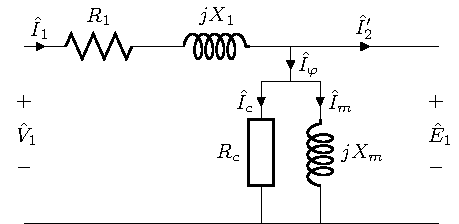
\includegraphics{figTransformersModelSecondPart}
\caption{ٹرانسفارمر مساوی دور، حصہ دوم۔}
\label{شکل_ٹرانسفارمر_ماڈل_حصہ_دوم}
\end{figure}

\جزوحصہ{ثانوی لچھے کی امالی برقی دباو}
قالب میں مشترکہ مقناطیسی بہاو ثانوی لچھے میں امالی برقی دباو \عددیء{\hat{E}_2} پیدا کرے گی اور چونکہ یہی مقناطیسی بہاو ابتدائی لچھے میں \عددیء{\hat{E}_1}  امالی پیدا کرتی ہے لہٰذا
\begin{align}\label{مساوات_ٹرانسفارمر_دباو_رو_شرح}
\frac{\hat{E}_1}{\hat{E}_2}=\frac{N_1}{N_2}
\end{align}
مساوات \حوالہ{مساوات_ٹرانسفارمر_رو_ہیجان_ضیاع_اجزاع} اور مساوات \حوالہ{مساوات_ٹرانسفارمر_دباو_رو_شرح}  کو ایک کامل ٹرانسفارمر سے ظاہر کیا جا سکتا ہے۔ یہ شکل \حوالہ{شکل_ٹرانسفارمر_ماڈل_حصہ_ثوم}  میں دکھایا گیا ہے۔
\begin{figure}
\centering
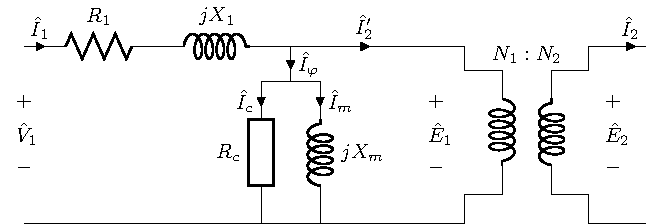
\includegraphics{figTransformersModelThirdPart}
\caption{ٹرانسفارمر مساوی دور، حصہ ثوم۔}
\label{شکل_ٹرانسفارمر_ماڈل_حصہ_ثوم}
\end{figure}

\جزوحصہ{ثانوی لچھے کی مزاحمت اور متعاملہ کے اثرات}
ثانوی لچھے کے سروں پر البتہ  \عددیء{\hat{E}_2} برقی دباو نہیں ہو گا چونکہ ثانوی لچھے کے، بالکل ابتدائی لچھے کی طرح، مزاحمت \عددیء{R_2}  اور متعاملہ  \عددیء{j X_2} ہوں گے جن میں ثانوی برقی رو \عددیء{\hat{I}_2}  کی وجہ سے برقی دباو گھٹے گا۔  لہٰذا ثانوی لچھے کے سروں پر برقی دباو \عددی{\hat{V}_2} قدرِ کم ہو گا۔ یعنی
\begin{align}
\hat{V}_2=\hat{E}_2-\hat{I}_2 R_2-j \hat{I}_2 X_2
\end{align}
	یوں حاصل ٹرانسفارمر کا مکمل مساوی دور یا \اصطلاح{ریاضی نمونہ}\فرہنگ{ریاضی نمونہ}\حاشیہب{mathematical model}\فرہنگ{model} شکل  \حوالہ{شکل_ٹرانسفارمر_مکمل_ماڈل} میں دکھایا گیا ہے۔
\begin{figure}
\centering
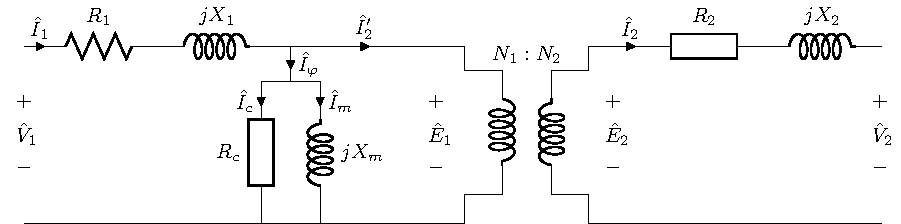
\includegraphics[width=0.9\linewidth]{figTransformersModelComplete}
\caption{ٹرانسفارمر کا مکمل مساوی دور یا ریاضی نمونہ۔}
\label{شکل_ٹرانسفارمر_مکمل_ماڈل}
\end{figure}

\جزوحصہ{رکاوٹ کا ابتدائی یا ثانوی جانب تبادلہ}
شکل \حوالہ{شکل_ٹرانسفارمر_مکمل_ماڈل}  میں دکھائے دور کے سب جزو کا تبادلہ ایک جانب سے دوسری جانب کیا جا سکتا ہے۔ یہ کرنے سے کامل ٹرانسفارمر کو مساوی دور کی بائیں یا دائیں جانب لے جایا جا سکتا ہے۔شکل \حوالہ{شکل_ٹرانسفارمر_مکمل_ماڈل_ابتدائی_جانب}   میں ثانوی جانب کی رکاوٹ کا ابتدائی جانب تبادلہ کیا گیا ہے جبکہ شکل  \حوالہ{شکل_ٹرانسفارمر_مکمل_ماڈل_ثانوی_جانب}  میں ابتدائی جانب کی رکاوٹ کا ثانوی جانب تبادلہ کیا گیا ہے۔اس طرح حاصل مساوی دور میں عموماً کامل ٹرانسفارمر بنایا ہی نہیں جاتا۔یہی شکل \حوالہ{شکل_ٹرانسفارمر_مکمل_ماڈل_ثانوی_جانب}   میں کیا گیا ہے۔

تبادلہ شدہ رکاوٹ  \عددیء{Z} کو \عددیء{Z'}  سے ظاہر کیا جاتا ہے۔یوں \عددیء{R_2} کے ٹرانسفارمر کی دوسری جانب تبادلہ کے بعد اسے \عددیء{R_2'} سے ظاہر کیا گیا ہے۔

ایسا دور استعمال کرتے وقت یہ ذہن میں رکھنا ہوتا ہے کہ ٹرانسفارمر کے کس جانب دور حل کیا جا رہا ہے۔
\begin{figure}
\centering
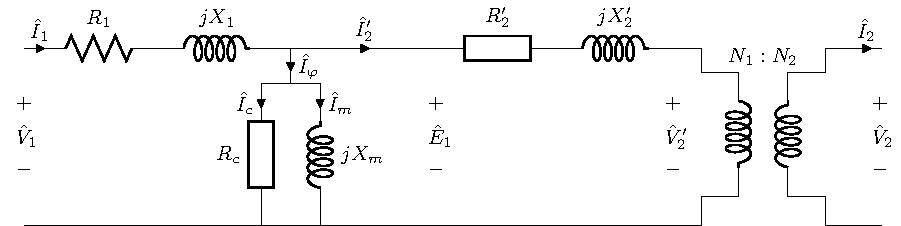
\includegraphics[width=0.9\linewidth]{figTransformersModelShiftedToPrimarySide}
\caption{ثانوی جانب رکاوٹ کا ابتدائی جانب تبادلہ کیا گیا ہے۔}
\label{شکل_ٹرانسفارمر_مکمل_ماڈل_ابتدائی_جانب}
\end{figure}
%
\begin{figure}
\centering
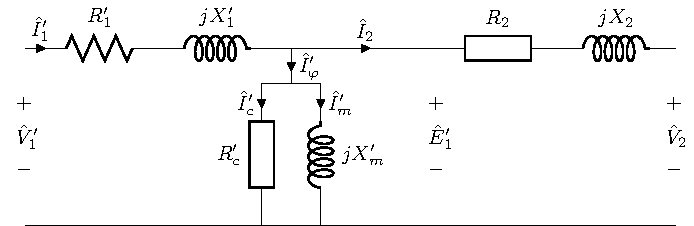
\includegraphics[width=0.9\linewidth]{figTransformersModelShiftedToSecondarySide}
\caption{ابتدائی جانب رکاوٹ کا ثانوی جانب تبادلہ کیا گیا ہے۔}
\label{شکل_ٹرانسفارمر_مکمل_ماڈل_ثانوی_جانب}
\end{figure}


%
\ابتدا{مثال}
ایک \عددیء{50} کلو وولٹ-ایمپیئر اور  \عددیء{2200:220} وولٹ برقی سکت کے ٹرانسفارمر کی زیادہ برقی دباو کی جانب کی رستا رکاوٹ \عددیء{Z_1=0.9+j 1.2}  اوہم اور کم برقی دباو کی جانب کی رِستا رکاوٹ \عددیء{Z_2=0.0089+j 0.011} اوہم ہے۔اگر اس کی \عددیء{R_c=\SI{6.4}{\kilo\ohm}} اور \عددیء{X_m=\SI{47}{\kilo\ohm}}  ہو تو اس کی شکل \حوالہ{شکل_ٹرانسفارمر_مکمل_ماڈل_ابتدائی_جانب}  اور شکل \حوالہ{شکل_ٹرانسفارمر_مکمل_ماڈل_ثانوی_جانب}  میں استعمال ہونے والے جزو معلوم کریں۔

	حل حصہ اول:
معلومات:
\begin{align*}
\SI{50}{\kilo \volt \ampere}, \quad \SI{50}{\hertz}, \quad 2200:220\,\textup{V}
\end{align*}
ٹرانسفارمر کے دونوں جانب کی برقی دباو لچھوں کے چکروں کی نسبت سے ہوتے ہیں لہٰذا
\begin{align*}
\frac{N_1}{N_2}=\frac{2200}{220}=\frac{10}{1}
\end{align*}
یوں اگر ٹرانسفارمر کی رکاوٹ کا زیادہ برقی دباو کی جانب تبادلہ کیا جائے تو
\begin{align*}
R_2'+j X_2' &=\left(\frac{N_1}{N_2} \right)^2 \left(R_2+j X_2 \right)\\
&=\left(\frac{10}{1} \right)^2 \left(0.0089+j 0.011 \right)\\
&=0.89+j 1.1
\end{align*}
جبکہ اس کی بقایا رکاوٹ وہی رہیں گے۔یوں شکل \حوالہ{شکل_ٹرانسفارمر_مکمل_ماڈل_ابتدائی_جانب}  کے جزو حاصل ہوئے۔

	حل حصہ دوم:
اگر مساوی دور کی رکاوٹ کا کم برقی دباو کی جانب تبادلہ کیا جائے تب
\begin{align*}
R_1'+j X_1' &=\left(\frac{N_2}{N_1} \right)^2 \left(R_1+j X_1 \right)\\
&=\left(\frac{1}{10} \right)^2 \left(0.9+j1.2 \right)\\
&=0.009+j0.012
\end{align*}
اسی طرح
\begin{align*}
R_c'&=\left(\frac{N_2}{N_1} \right)^2 R_c=64\\
X_m'&=\left(\frac{N_2}{N_1} \right)^2 X_m=470
\end{align*}
جبکہ \عددیء{Z_2} وہی رہے گا۔
\انتہا{مثال}
%
\جزوحصہ{ٹرانسفارمر کے سادہ ترین مساوی دور}
ایک انجنیئر کو جب ایک ٹرانسفارمر استعمال کرنا ہو تو وہ حساب کرتے وقت شکل \حوالہ{شکل_ٹرانسفارمر_مکمل_ماڈل_ابتدائی_جانب}  میں دیئے گئے دور کو استعمال کر سکتا ہے۔ یہ دور حقیقی ٹرانسفارمر کی بہت اچھی عکاسی کرتا ہے۔ البتہ جہاں ہمیں نہایت صحیح جواب مطلوب نہ ہوں وہاں اس دور کی سادہ اشکال بھی استعمال کی جا سکتیں ہیں۔ اس باب میں ہم ایسے ہی سادہ مساوی دوروں کا ذکر کریں گے۔
\begin{figure}
\centering
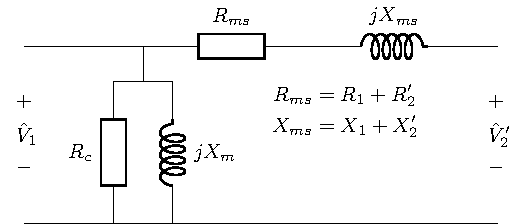
\includegraphics[width=0.9\linewidth]{figTransformersModelLeftHand}
\caption{\عددیء{R_c} اور \عددیء{jX_m} کو بائیں جانب منتقل کیا گیا ہے۔}
\label{شکل_ٹرانسفارمر_بائیں_جانب}
\end{figure}
%
\begin{figure}
\centering
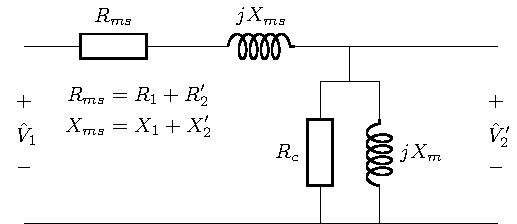
\includegraphics[width=0.9\linewidth]{figTransformersModelRightHand}
\caption{\عددیء{R_c} اور \عددیء{jX_m} کو دائیں جانب منتقل کیا گیا ہے۔}
\label{شکل_ٹرانسفارمر_دائیں_جانب}
\end{figure}

شکل  \حوالہ{شکل_ٹرانسفارمر_مکمل_ماڈل_ابتدائی_جانب} میں \عددیء{R_c} اور \عددیء{X_m} کو بائیں یا دائیں طرف لے جانے سے  شکل  \حوالہ{شکل_ٹرانسفارمر_بائیں_جانب}  اور  شکل \حوالہ{شکل_ٹرانسفارمر_دائیں_جانب}  حاصل ہوتے ہیں۔چونکہ \عددیء{\hat{I}_\varphi} کی مقدار نہایت کم\حاشیہد{\عددیء{\hat{I}_\varphi} ٹرانسفارمر کے کُل برقی بوجھ کے صرف دو سے چھ فی صد ہوتی ہے}  ہوتی ہے اس لئے ایسا  کرنے سے حاصل جواب پر کوئی خاص فرق نہیں پڑتا۔ چونکہ اس شکل میں \عددیء{R_1} ،\عددیء{R_2'}، \عددیء{X_1}  اور \عددیء{X_2'} سلسلہ وار ہیں اس لئے ان کو جمع کیا جا سکتا ہے شکل میں ان کو مساوی مزاحمت \عددیء{R_{ms}}  اور مساوی متعاملہ \عددیء{X_{ms}} کہا گیا ہے۔اسی قسم کے ادوار  شکل  \حوالہ{شکل_ٹرانسفارمر_مکمل_ماڈل_ثانوی_جانب} سے بھی حاصل ہوتے  ہیں۔

ہم ایک قدم اور آگے جا سکتے ہیں اور \عددیء{\hat{I}_\varphi} کو مکمل طور پر نظر انداز کر سکتے ہیں یعنی اس کو ہم صفر تصور کر لیتے ہیں۔اس کا مطلب ہے کہ مساوی دور میں \عددیء{R_c} اور \عددیء{j X_m} دونوں کو کھلے دور کیا جاتا ہے  یعنی انہیں مساوی دور سے ہٹا دیا جاتا ہے۔ شکل \حوالہ{شکل_ٹرانسفارمر_سادہ_ماڈل}-الف  میں ایسا کیا گیا ہے۔اس دور میں قالب کے اثرات کو مکمل طور پر نظرانداز کیا گیا ہے۔

بیشتر وقت ہمیں اس سے بھی کم صحیح جواب مطلوب ہوتا ہے۔چونکہ \عددیء{X_m\gg R_c}  لہٰذا ہم  \عددیء{R_{ms}} کو بھی نظرانداز کر سکتے ہیں۔یوں شکل \حوالہ{شکل_ٹرانسفارمر_سادہ_ماڈل}-ب حاصل ہوتا ہے۔
\begin{figure}
\centering
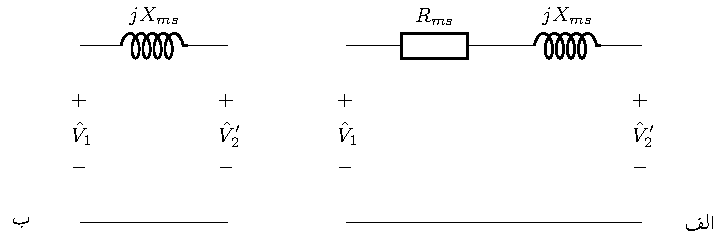
\includegraphics[width=0.9\linewidth]{figTransformersModelCoreLossNeglected}
\caption{ٹرانسفارمر کے سادہ مساوی ادوار۔}
\label{شکل_ٹرانسفارمر_سادہ_ماڈل}
\end{figure}
\حصہ{کھلے دور معائنہ اور کسرِ دور معائنہ}
پچھلے حصے میں بیان کئے گئے ٹرانسفارمر کے مساوی دور کے جزو ٹرانسفارمر کے دو معائنوں سے حاصل کئے جا سکتے ہیں۔ ان معائنوں کو کھلے دور معائنہ اور کسرِ دور معائنہ کہتے ہیں۔اس حصے میں انہیں پر غور کیا جائے گا۔

\جزوحصہ{کھلے دور معائنہ}
کھلے  دور معائنہ\فرہنگ{معائنہ!کھلے دور}\حاشیہب{open circuit test}\فرہنگ{open circuit test} جیسا کہ نام سے واضح  ہے،  ٹرانسفارمر کی ایک جانب لچھے کے سروں کو آزاد رکھ کر کیا جاتا ہے۔ یہ معائنہ اتنی برقی دباو اور تعدد یا ان کے قریب ترین مقداروں پر کیا جاتا ہے جتنے پر ٹرانسفارمر کی بناوٹ\فرہنگ{بناوٹ}\حاشیہب{design} ہو۔ اگرچہ یہ معائنہ ٹرانسفارمر کے کسی بھی جانب کے لچھے پر کیا جا سکتا ہے، حقیقت میں اسے کم برقی دباو والی جانب کے لچھے پر کرنا آسان ہوتا ہے۔یہ بات ایک مثال سے زیادہ آسانی سے سمجھ آتی ہے۔

	مثلاً  ہم  \عددیء{\SI{25}{\kilo \volt \ampere}} اور \عددیء{11000:220\,\textup{V}}  کا \عددیء{\SI{50}{\hertz}} پر چلنے والے ایک دور کے ٹرانسفارمر کا معائنہ کرنا چاہتے ہیں۔ اگر یہ معائنہ اس کے گیارہ ہزار کے لچھے پر  کیا جائے تو گیارہ ہزار برقی دباو کے لگ بھگ برقی دباو استعمال کیا جائے گا اور اگر دو سو بیس برقی دباو والے لچھے پر کیا جائے تو دو سو بیس برقی دباو کے لگ بھگ برقی دباو  استعمال کیا جائے گا۔ دونوں صورتوں میں تعدد \عددیء{\SI{50}{\hertz}} کے لگ بھگ رکھا جائے گی۔\عددیء{\SI{11}{\kilo \volt}} کی برقی دباو پر کام کرنا نہایت خطرناک ثابت ہو سکتا ہے۔یہی وجہ ہے کہ اس معائنہ کو کم برقی دباو والے لچھے پر ہی کیا جاتا ہے۔

 جس برقی دباو پر ٹرانسفارمر عام حالات میں استعمال ہوتا ہے اس معائنہ میں کم برقی دباو والی جانب کے لچھے پر اتنے ہی یا اس کی قریب مقدار کی برقی دباو \عددیء{V_t} لاگو کر کے کھلے دور برقی طاقت \عددیء{p_t} اور  کھلے دور برقی رو \عددیء{I_t}  ناپے جاتے ہیں۔معائنہ حقیقت میں استعمال کے دوران برقی دباو کے جتنے قریب برقی دباو پر کیا جائے اتنا بہتر جواب حاصل ہوتا ہے۔ ٹرانسفارمر کی دوسری جانب لچھے کے سرے چونکہ آزاد رکھے جاتے ہیں اس لئے اس میں  برقی رو صفر ہو گا۔  لہٰذا ناپا گیا برقی رو صرف ہیجان انگیز برقی رو \عددیء{\hat{I}_\varphi} ہو گا۔ ٹرانسفارمر جتنی برقی رو کے لئے بنایا گیا ہو یہ برقی رو اس  کے تقریباً دو سے چھ  فی صد ہوتا ہے۔شکل \حوالہ{شکل_ٹرانسفارمر_مکمل_ماڈل_ابتدائی_جانب}   کو مدِ نظر رکھتے ہوئے اگر ہم بائیں جانب کو کم برقی دباو والی جانب تصور کریں تو شکل میں \عددیء{V_t} کو  \عددیء{V_1} کی جگہ لاگو کرنا ہو گا۔یوں ہم جو برقی رو ناپیں گے وہ  غیر سمتی\حاشیہب{scalar} \عددیء{I_1}  ہو گا۔ چونکہ  \عددیء{I_2'} صفر کے برابر ہے لہٰذا \عددیء{I_1}  درحقیقت \عددیء{\hat{I}_\varphi} کے مقدار \عددیء{I_\varphi} کے برابر ہو گا۔ یعنی  اس  طرح
\begin{align*}
I_t=I_1=I_\varphi
\end{align*}
اتنی کم برقی رو سے لچھے کی رکاوٹ میں نہایت کم برقی دباو گھٹتا ہے،لہٰذا اسے نظر انداز کیا جاتا ہے یعنی
\begin{align*}
V_{R1}&=I_t R_1=I_\varphi R_1 \approx 0\\
V_{X1}&=I_1 X_1=I_\varphi X_1 \approx 0
\end{align*}
یوں  \عددیء{R_c}  اور \عددیء{X_m} پر  تقریباً \عددیء{V_t} برقی دباو پایا جائے گا۔ یہ شکل \حوالہ{شکل_ٹرانسفارمر_مکمل_ماڈل_ابتدائی_جانب}  سے ظاہر ہے۔ان حقائق کو مد نظر رکھتے ہوئے شکل \حوالہ{شکل_ٹرانسفارمر_کھلے_سرے_معائنہ} حاصل ہوتا ہے۔
\begin{figure}
\centering
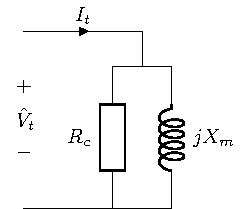
\includegraphics{figTransformersOpenCircuitTest}
\caption{کھلے سرے معائنہ۔}
\label{شکل_ٹرانسفارمر_کھلے_سرے_معائنہ}
\end{figure}

چونکہ برقی طاقت کا ضیاع صرف مزاحمت میں ہی ممکن ہے لہٰذا \عددیء{p_t} صرف  \عددیء{R_c}  میں ہی ضائع ہو گی۔ یوں
\begin{align*}
p_t=\frac{V_t^2}{R_c}
\end{align*}
لکھا جائے گا۔یوں
\begin{align}\label{مساوات_ٹرانسفارمر_کھلے_دور_مزاحمت_حاصل}
R_c&=\frac{V_t^2}{p_t}
\end{align}
حاصل ہوتا ہے۔

اسی طرح چونکہ برقی دباو اور برقی رو کی مقداروں کے تناسب کو برقی رکاوٹ کی مقدار کہتے ہیں لہٰذا
\begin{align*}
\abs{Z_t}=\frac{V_t}{I_t}
\end{align*}
مگر شکل \حوالہ{شکل_ٹرانسفارمر_کھلے_سرے_معائنہ}  سے واضح ہے کہ
\begin{align*}
\frac{1}{Z_t}=\frac{1}{R_c}+\frac{1}{j X_m}
\end{align*}
لہٰذا
\begin{align*}
Z_t&=\frac{j R_c X_m}{R_c+j X_m}\\
\abs{Z_t}&=\frac{R_c X_m}{\sqrt{R_c^2+X_m^2}}
\end{align*}
جس سے حاصل ہوتا ہے
\begin{align}\label{مساوات_ٹرانسفارمر_کھلے_دور_امالہ_حاصل}
X_m=\frac{R_c \abs{Z_t}}{\sqrt{R_c^2-\abs{Z_t}^2}}
\end{align}
مساوات \حوالہ{مساوات_ٹرانسفارمر_کھلے_دور_مزاحمت_حاصل}  سے \عددیء{R_c} اور  مساوات \حوالہ{مساوات_ٹرانسفارمر_کھلے_دور_امالہ_حاصل}  سے  \عددیء{X_m}  کا حساب لگایا جاتا ہے۔

یاد رہے کہ حاصل کردہ \عددیء{R_c} اور \عددیء{X_m} ٹرانسفارمر کے اسی جانب کے لئے درست ہیں جس جانب انہیں حاصل کیا گیا ہو۔اگر ان کی قیمتیں دوسری جانب درکار ہوں تب تبادلہ رکاوٹ کا استعمال کرتے ہوئے اس جانب کی قیمتیں حاصل کی جا سکتی ہیں۔ 

\جزوحصہ{ کسرِ دور معائنہ}
یہ معائنہ بھی پچھلے معائنہ کی طرح ٹرانسفارمر کے کسی بھی طرف کیا جا سکتا ہے مگر حقیقت میں اسے زیادہ برقی دباو کے لچھے پر ہی کرنا زیادہ آسان ہوتا ہے۔ یہ معائنہ جتنے برقی رو کے لئے ٹرانسفارمر بنایا گیا ہو اتنی برقی رو یا اس کے قریب مقدار پر کیا جاتا ہے۔یعنی اس معائنہ میں کوشش ہوتی ہے کہ ٹرانسفارمر کے لچھے میں اتنی برقی رو گزرے جتنی کے لئے یہ بنایا گیا ہو۔ لہٰذا اگر ہم پچھلے معائنہ میں استعمال ہونے والے ٹرانسفارمر کی بات آگے بڑھائیں تو اس کا زیادہ برقی دباو کا لچھا \عددیء{\SI{2.2727}{\ampere}} اور کم برقی دباو کا لچھا \عددیء{\SI{113.63}{\ampere}} کے لئے بنایا گیا ہے۔ لہٰذا اگر یہ معائنہ کم برقی دباو لچھے پر کیا جائے تو اسے \عددیء{\SI{113.63}{\ampere}}  پر  کرنا ہو گا اور اگر زیادہ برقی دباو لچھے پر کیا جائے تو صرف \عددیء{\SI{2.2727}{\ampere}} پر کرنا ہو گا جو کہ زیادہ آسان ہے۔
\begin{figure}
\centering
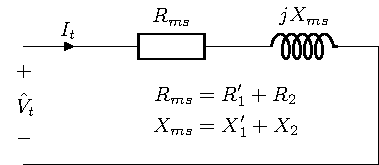
\includegraphics{figTransformersShortCircuitTest}
\caption{کسر دور معائنہ۔}
\label{شکل_ٹرانسفارمر_کسر_دور_معائنہ}
\end{figure}

اس معائنہ میں کم برقی دباو لچھے کے دونوں سروں کو آپس میں جوڑا جاتا ہے یعنی انہیں کسرِ دور کر لیا جاتا ہے اور زیادہ برقی دباو لچھے پر اس جانب کی ڈیزائن کردہ برقی دباو کے دو سے بارہ  فی صد کا برقی دباو \عددیء{V_t} لاگو کر کے کسرِ دور برقی رو \عددیء{I_t} اور کسرِ دور برقی طاقت \عددیء{p_t} ناپے جاتے ہیں۔ جس لچھے کے سرے آپس میں کسرِ دور ہوتے ہیں اس میں سے برقی رو گزرتی ہے اور اس کا عکس دوسری جانب بھی موجود ہوتا ہے۔ یہ برقی رو ٹرانسفارمر کے ڈیزائن کردہ برقی رو کے لگ بھگ ہوتا ہے۔ اس معائنہ کا دور شکل \حوالہ{شکل_ٹرانسفارمر_کسر_دور_معائنہ} میں دکھایا گیا ہے۔کھلے سرے معائنے کی طرح اگر کسر دور معائنے میں بھی  شکل \حوالہ{شکل_ٹرانسفارمر_مکمل_ماڈل_ابتدائی_جانب} کے بائیں جانب کو کم برقی دباو والی جانب تصور کریں تو  \عددیء{V_t} کو  \عددیء{V_2} کی جگہ لاگو کرنا ہو گا۔

 چونکہ یہ معائنہ بہت کم برقی دباو پر کیا جاتا ہے لہٰذا اس معائنہ میں ہیجان انگیز برقی رو کو مکمل طور پر نظرانداز کیا جا سکتا ہے۔ شکل سے ہم دیکھتے ہیں کہ چونکہ برقی طاقت صرف مزاحمت میں ہی ضائع ہو سکتی ہے لہٰذا
\begin{align*}
p_t=I_t^2 \left(R_{ms}\right)
\end{align*}
ہو گا جس سے
\begin{align}\label{مساوات_ٹرانسفارمر_کسر_دور_مزاحمت_حاصل}
R_{ms}=\frac{p_t}{I_t^2}
\end{align}
حاصل ہوتا ہے۔

کسرِ دور برقی رو اور برقی دباو سے ہمیں ملتی ہے
\begin{align*}
\abs{Z_t}=\frac{V_t}{I_t}
\end{align*}
مگر شکل سے واضح ہے کہ
\begin{align*}
Z_t&=R_{ms}+j X_{ms}\\
\abs{Z_t}&=\sqrt{R_{ms}^2+X_{ms}^2}
\end{align*}
لہٰذا
\begin{align}\label{مساوات_ٹرانسفارمر_کسر_دور_امالہ_حاصل}
X_{ms}=\sqrt{\abs{Z_t}^2-R_{ms}^2}
\end{align}
مساوات \حوالہ{مساوات_ٹرانسفارمر_کسر_دور_مزاحمت_حاصل} کُل مزاحمت دیتا ہے البتہ اس سے \عددی{R_1} یا \عددیء{R_2} حاصل نہیں کیا جا سکتا۔اسی طرح مساوات \حوالہ{مساوات_ٹرانسفارمر_کسر_دور_امالہ_حاصل} سے \عددیء{X_1} اور \عددیء{X_2} علیحدہ نہیں کئے جا سکتے۔کسر دور معائنہ سے اتنی ہی معلومات حاصل کرنا ممکن ہے۔حقیقت میں اتنی معلومات کافی ہوتی ہے۔ اگر ان اجزاء ک علیحدہ علیحدہ قیمتیں درکار ہوں تو ایسی صورت میں تصور کیا جاتا ہے کہ
\begin{align*}
R_1'&=R_2\\
X_1'&=X_2
\end{align*}
ہیں۔

 چونکہ یہ معائنہ عموماً جہاں ٹرانسفارمر موجود ہو وہیں کرنا پڑتا ہے لہٰذا یہ ممکن نہیں ہوتا کہ ٹرانسفارمر کو بالکل اتنا برقی دباو دیا جائے جتنا درکار ہو بلکہ جو برقی دباو موجود ہو اسی سے کام چلانا پڑتا ہے۔ لیکن اس بات کا خیال بہت ضروری ہے کہ جو برقی دباو ٹرانسفارمر کو دیا جا رہا ہو وہ ڈیزائن کردہ برقی دباو کے دو سے بارہ  فی صد ہو۔ مثلاً اگر اسی \عددیء{11000:220\,\textup{V}} ٹرانسفارمر کی بات کی جائے تو اس کے زیادہ برقی دباو لچھے پر \عددیء{\SI{220}{\volt}} اور \عددیء{\SI{1320}{\volt}}  کے درمیان کوئی بھی برقی دباو دیا جا سکتا ہے۔ چونکہ ہمارے ہاں \عددیء{\SI{220}{\volt}}  اور \عددیء{\SI{440}{\volt}}  عام پائے جاتے ہیں لہٰذا ہم \عددیء{\SI{220}{\volt}}  یا \عددیء{\SI{440}{\volt}}  ہی استعمال کریں گے۔

یہاں یہ ایک مرتبہ دوبارہ یاد دھیانی کراتا جاول کہ ٹرانسفارمر کی ایک جانب لچھے کے سرے آپس میں جوڑ کر، یعنی انہیں کسرِ دور کر کے، دوسری جانب لچھے پر کسی بھی صورت میں اس جانب کی پوری برقی دباو لاگو نہیں کرنا۔ ایسا کرنا  شدید  خطرناک اور جان لیوا ثابت ہو سکتا ہے۔

یاد رہے کہ حاصل کردہ \عددیء{R_c} اور \عددیء{X_m} ٹرانسفارمر کے اسی جانب کے لئے درست ہیں جس جانب انہیں حاصل کیا گیا ہو۔اگر ان کی قیمتیں دوسری جانب درکار ہوں تب تبادلہ رکاوٹ کا استعمال کرتے ہوئے اس جانب کی قیمتیں حاصل کی جا سکتی ہیں۔ 
%
\ابتدا{مثال}
ایک \عددیء{25}  کلو وولٹ-ایمپیئر، \عددیء{11000:220} وولٹ اور \عددیء{50} ہرٹز پر چلنے والے ٹرانسفارمر کے کھلے دور اور کسرِ دور معائنہ کئے جاتے ہیں جن کے نتائج یہ ہیں۔
\begin{itemize}
\item
کھلے دور معائنہ کرتے وقت کم برقی دباو کی جانب  \عددیء{\SI{220}{\volt}} لاگو کئے جاتے ہیں۔اسی جانب برقی رو \عددیء{\SI{39.64}{\ampere}} اور طاقت کا ضیاع \عددیء{\SI{600}{\watt}} ناپے جاتے ہیں۔
\item
کسرِ دور معائنہ کرتے وقت زیادہ برقی دباو کی جانب  \عددیء{\SI{440}{\volt}} لاگو کئے جاتے ہیں۔اسی جانب برقی رو \عددیء{\SI{2.27}{\ampere}} اور طاقت کا ضیاع \عددیء{\SI{560}{\watt}} ناپے جاتے ہیں۔
\end{itemize}

کھلے دور حل:
\begin{align*}
\abs{Z_t}&=\frac{220}{39.64}=\SI{5.55}{\ohm}\\
R_c&=\frac{220^2}{600}=\SI{80.67}{\ohm}\\
X_m&=\frac{80.67 \times 5.55}{\sqrt{80.67^2-5.55^2}}=\SI{5.56}{\ohm}
\end{align*}
کسر دور حل:
\begin{align*}
Z_t&=\frac{440}{2.27}=\SI{193.83}{\ohm}\\
R_{ms}&=\frac{560}{2 \times 2.27^2}=\SI{108.68}{\ohm}\\
X_{ms}&=\sqrt{193.83^2-108.68^2}=\SI{160}{\ohm}
\end{align*}

ان نتائج کو کم برقی دباو جانب منتقل کرتے ہوئے 
\begin{align*}
\left(\frac{220}{11000} \right)^2 \times 108.68=\SI{43.47}{\milli \ohm}\\
\left(\frac{220}{11000} \right)^2 \times 160=\SI{64}{\milli \ohm}
\end{align*}
یعنی
\begin{align*}
R_1&=R_2'=\frac{\SI{43.47}{\milli \ohm}}{2}=\SI{21.7}{\milli \ohm}\\
X_1&=X_2'=\frac{\SI{64}{\milli \ohm}}{2}=\SI{32}{\milli \ohm}
\end{align*}
حاصل ہوتا ہے۔ان نتائج سے حاصل کم برقی دباو جانب مساوی دور شکل \حوالہ{شکل_ٹرانسفارمر_کھلے_سرے_کسر_دور_مثال} میں دکھایا گیا ہے۔
\begin{figure}
\centering
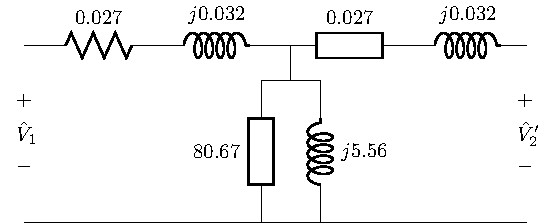
\includegraphics{figTransformersOpenAndShortTestExample}
\caption{کھلے دور اور کسرِ دور معائنہ سے کم برقی دباو جانب  مساوی دور۔}
\label{شکل_ٹرانسفارمر_کھلے_سرے_کسر_دور_مثال}
\end{figure}
\انتہا{مثال}
%
\حصہ{تین مرحلہ ٹرانسفارمر}
اب تک ہم  \اصطلاح{ایک مرحلہ}\حاشیہب{single phase} ٹرانسفارمر پر غور کرتے رہے ہیں۔حقیقت میں برقی طاقت کی منتقلی میں عموماً \اصطلاح{تین مرحلہ}\فرہنگ{تین مرحلہ}\حاشیہب{three phase}\فرہنگ{three phase} ٹرانسفارمر استعمال ہوتے ہیں۔تین مرحلہ ٹرانسفارمر یکساں تین عدد  ایک مرحلہ  ٹرانسفارمر اکٹھے رکھ کر بنایا جا سکتا ہے۔یوں اگر ایک ٹرانسفارمر خراب ہو جائے تو اس کو ٹھیک ہونے کے لئے ہٹا کر بقایا دو ٹرانسفارمر دوبارہ چالو کئے جا سکتے ہیں۔تین مرحلہ ٹرانسفارمر بنانے کا اس سے بہتر طریقہ شکل \حوالہ{شکل_ٹرانسفارمر_ایک_مرکز_تین-ٹرانسفارمر} میں دکھایا گیا ہے جہاں ایک ہی مقناطیسی قالب پر تینوں ٹرانسفارمر کے لچھے لپٹے گئے ہیں۔اس شکل میں \عددیء{\hat{V}_{i1}} پہلے ٹرانسفارمر کا ابتدائی لچھا جبکہ \عددیء{\hat{V}_{s1}} اس کا ثانوی لچھا ہے۔اس طرح کے تین مرحلہ ٹرانسفارمر سستے، ہلکے اور چھوٹے ہونے کی وجہ سے عام ہو گئے ہیں اور آپ کو روز مرہ زندگی میں یہی نظر آئیں گے۔ان میں برقی ضیاع بھی قدرِ کم ہوتی ہے۔
\begin{figure}
\centering
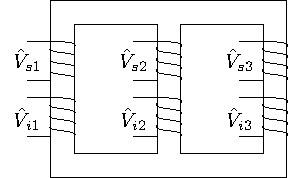
\includegraphics{figTransformersThreePhaseSingleCore}
\caption{ایک ہی قالب پر تین ٹرانسفارمر۔}
\label{شکل_ٹرانسفارمر_ایک_مرکز_تین-ٹرانسفارمر}
\end{figure}

شکل \حوالہ{شکل_ٹرانسفارمر_ستارہ_تکونی_جوڑ}-الف میں تین ٹرانسفارمر دکھائے گئے ہیں۔ان تین ٹرانسفارمر کے ابتدائی لچھے آپس میں دو طریقوں سے جوڑے جا سکتے ہیں۔ایک کو \اصطلاح{ستارہ نما} جوڑ\فرہنگ{ستارہ نما جوڑ}\فرہنگ{جوڑ!ستارہ نما}\حاشیہب{star connected}\فرہنگ{star connected} \عددیء{Y}  اور دوسرے کو \اصطلاح{تکونی} جوڑ\فرہنگ{تکونی جوڑ}\فرہنگ{جوڑ!تکونی}\حاشیہب{delta connected}\فرہنگ{delta connected}  \عددیء{\Delta}   کہتے ہیں۔اسی طرح ان تینوں ٹرانسفارمروں کے ثانوی  لچھے انہیں دو طریقوں سے جوڑے جا سکتے ہیں۔یوں انہیں جوڑنے کے چار ممکنہ طریقے ہیں یعنی
\begin{itemize}
\item
ستارہ:تکونی  \quad \عددیء{Y:\Delta}
\item
ستارہ:ستارہ \quad  \عددیء{Y:Y}
\item
تکونی:تکونی \quad  \عددیء{\Delta:\Delta}
\item
تکونی:ستارہ  \quad  \عددیء{\Delta:Y}
\end{itemize}

شکل \حوالہ{شکل_ٹرانسفارمر_ستارہ_تکونی_جوڑ}-الف میں ان تین ٹرانسفارمروں کے ابتدائی لچھوں کو ستارہ نما جوڑا گیا ہے جبکہ ان کی ثانوی لچھوں کو تکونی جوڑا گیا ہے۔شکل-ب میں تینوں ٹرانسفارمر کی ابتدائی لچھوں کو  ستارہ نما  دکھایا گیا ہے۔اسی طرح ثانوی لچھوں کو تکونی  دکھایا گیا ہے۔انہی شکلوں کی وجہ سے ان کو ستارہ نما جوڑ اور تکونی جوڑ کہتے ہیں۔

ایسی شکل بناتے وقت تینوں ٹرانسفارمروں کے ابتدائی لچھے کو جس زاویہ پر بنایا جاتا ہے اس کے ثانوی لچھے کو بھی اُسی زاویہ پر بنایا جاتا ہے۔یوں شکل کے حصہ الف میں سب سے اوپر ٹرانسفارمر جس کے ابتدائی جانب کے  سرے \عددیء{an} اور ثانوی جانب  کے سرے \عددیء{a'n'} ہیں کو حصہ با میں صفر زاویہ پر بنایا گیا ہے۔تین  مرحلہ ٹرانسفارمروں کو اس طرح کی علامتوں سے ظاہر کیا جاتا ہے اور ان میں قالب نہیں دکھایا جاتا۔

ٹرانسفارمر کے جوڑ بیان کرتے وقت بائیں جانب کے جوڑ کو پہلے اور دائیں جانب کی جوڑ کو بعد میں پکارتے ہیں۔یوں شکل میں ٹرانسفارمر کو ستارہ-تکونی جُڑا ٹرانسفارمر کہیں گے۔اسی طرح ابتدائی جانب کو بائیں اور ثانوی جانب کو دائیں ہاتھ بنایا جاتا ہے۔یوں اس شکل میں ابتدائی جانب ستارہ نما ہے جبکہ ثانوی جانب تکونی ہے۔
\begin{figure}
\centering
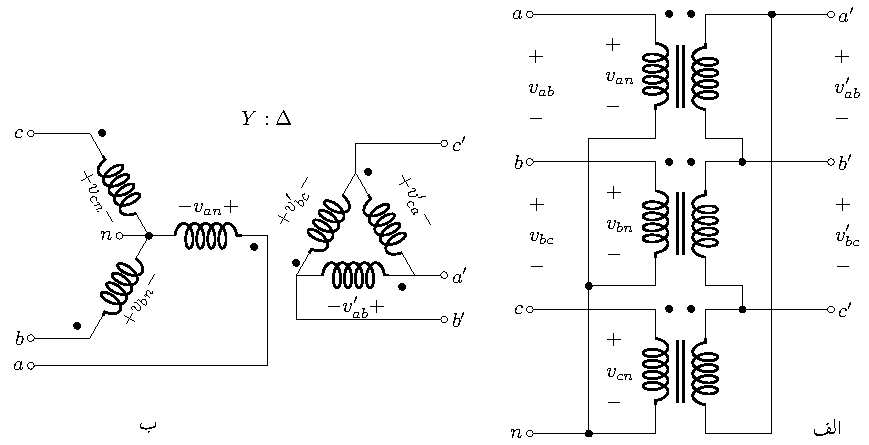
\includegraphics[width=\linewidth]{figTransformersStarDeltaConnections}
\caption{تین مرحلہ ستارہ-تکونی ٹرانسفارمر}
\label{شکل_ٹرانسفارمر_ستارہ_تکونی_جوڑ}
\end{figure}


	ستارہ نما جڑی جانب سے چار برقی تاریں نکلتی ہیں۔اس جانب لچھوں کے مشترکہ سرا \عددیء{n} کو عموماً ٹرانسفارمر کے نزدیک زمین میں گہرائی تک دھنسا دیا جاتا ہے۔اس تار کو \اصطلاح{زمینی تار}\فرہنگ{زمینی تار}\حاشیہب{ground}\فرہنگ{ground wire}  یا صرف \اصطلاح{زمین}\فرہنگ{زمین}\حاشیہب{ground, earth,neutral}\فرہنگ{earth}  کہتے ہیں۔عام فہم میں اسے \اصطلاح{ٹھنڈی تار}\فرہنگ{ٹھنڈی تار}\حاشیہب{neutral} کہتے ہیں۔باقی تین یعنی \عددیء{a,b,c}  \اصطلاح{گرم تار}\فرہنگ{گرم تار}\حاشیہب{live wires} کہلاتے ہیں۔

ٹرانسفارمر کی لچھے پر برقی دباو کو \اصطلاح{یک مرحلہ برقی دباو}\فرہنگ{یک مرحلہ برقی دباو} \عددیء{\hat{V}_{\textup{یکمرحلہ}}}\حاشیہب{phase voltage}\فرہنگ{phase voltage} کہتے ہیں اور لچھے میں برقی رو کو \اصطلاح{یک مرحلہ برقی رو}\فرہنگ{یک مرحلہ برقی رو} \عددیء{\hat{I}_{\textup{یکمرحلہ}}}\حاشیہب{phase current}\فرہنگ{phase current}  کہتے ہیں۔ جبکہ ٹرانسفارمر سے باہر نکلتی کسی دو گرم تاروں کے مابین برقی دباو کو \اصطلاح{تار کی برقی دباو}\فرہنگ{تار کی برقی دباو} \عددیء{\hat{V}_{\textup{تار}}}\حاشیہب{line to line voltage}\فرہنگ{line voltage} کہتے ہیں اور کسی بھی گرم تار میں برقی رو کو \اصطلاح{تار کی برقی رو}\فرہنگ{تار کی برقی رو} \عددیء{\hat{I}_{\textup{تار}}}\حاشیہب{line current}\فرہنگ{line current}  کہتے ہیں۔ زمینی تار میں برقی رو کو \اصطلاح{زمینی برقی رو}\فرہنگ{زمینی برقی رو}  \عددیء{\hat{I}_{\textup{زمینی}}}\حاشیہب{ground current}\فرہنگ{ground current} کہتے ہیں۔

ستارہ نما \عددیء{Y} جانب \اصطلاح{یک مرحلہ} مقداروں اور \اصطلاح{تار} کی مقداروں  کا آپس میں یوں رشتہ ہے
\begin{gather}
\begin{aligned}\label{مساوات_ستارہ_ٹرانسفارمر_تار_اور_دور_رشتے}
V_{\textup{تار}}&=\sqrt{3} V_{\textup{یکمرحلہ}}\\
I_{\textup{تار}}&=I_{\textup{یکمرحلہ}}
\end{aligned}
\end{gather}
جبکہ تکونی \عددیء{\Delta} جانب یک مرحلہ اور تار کی مقداروں کا آپس میں یوں رشتہ ہے
\begin{gather}
\begin{aligned}\label{مساوات_تکونی_ٹرانسفارمر_تار_اور_دور_رشتے}
V_{\textup{تار}}&= V_{\textup{یکمرحلہ}}\\
I_{\textup{تار}}&=\sqrt{3} I_{\textup{یکمرحلہ}}
\end{aligned}
\end{gather}
یہ مرحلی سمتیہ کے رشتے نہیں بلکہ ان کی غیر سمتی قیمتوں کے رشتے ہیں۔ان دو مساواتوں سے حاصل ہوتا ہے
\begin{align}
V_{\textup{تار}} I_{\textup{تار}}=\sqrt{3} V_{\textup{یکمرحلہ}} I_{\textup{یکمرحلہ}}
\end{align}
چونکہ ایک مرحلہ ٹرانسفارمر کی وولٹ-ایمپیئر \عددیء{V_{\textup{یکمرحلہ}} I_{\textup{یکمرحلہ}}} ہیں اور ایسے تین ٹرانسفارمر مل کر ایک تین مرحلہ ٹرانسفارمر بناتے ہیں لہٰذا تین  مرحلہ ٹرانسفارمر کی وولٹ-ایمپیئر اس کے تین گنا ہوں گے یعنی
\begin{align}
\textup{وولٹ-ایمپیئر}= 
3 V_{\textup{یکمرحلہ}} I_{\textup{یکمرحلہ}}= 
3 \times \frac{V_{\textup{تار}} I_{\textup{تار}}}{\sqrt{3}}=
\sqrt{3} V_{\textup{تار}} I_{\textup{تار}}
\end{align}
یہ مساوات \اصطلاح{تین مرحلہ} ادوار  میں عام استعمال ہوتی ہے۔

	ٹرانسفارمر کسی طرح بھی جوڑے جائیں وہ اپنی بنیادی کارکردگی تبدیل نہیں کرتے لہٰذا انہیں ستارہ نما یا تکونی جوڑنے کے بعد بھی ان میں ہر ایک ٹرانسفارمر انفرادی طور پر صفحہ \حوالہصفحہ{مساوات_ٹرانسفارمر_تبادلہ_دباو_رو} پر دئے مساوات \حوالہ{مساوات_ٹرانسفارمر_تبادلہ_دباو_رو}  اور صفحہ \حوالہصفحہ{مساوات_ٹرانسفارمر_متبادل_رکاوٹ_تعریف} پر دئے مساوات \حوالہ{مساوات_ٹرانسفارمر_متبادل_رکاوٹ_تعریف}  پر پورے اترے گا۔انہیں استعمال کر کے شکل \حوالہ{شکل_ٹرانسفارمر_تین_دور_ٹرانسفارمر_کے_مختلف_جوڑ}  میں دیئے گئے ٹرانسفارمروں کے ابتدائی اور ثانوی جانب کی یک مرحلہ اور تار کی مقداروں کے رشتے حاصل کئے جا سکتے ہیں۔اس شکل میں \عددیء{a=N_1/N_2} ہے جہاں  \عددیء{N_1:N_2} ان میں ایک مرحلہ ٹرانسفارمر کے چکر کی نسبت ہے۔تین مرحلہ ٹرانسفارمر پر لگی تختی پر دونوں جانب تار کی برقی دباو کی نسبت لکھی جاتی ہے۔
\begin{figure}
\centering
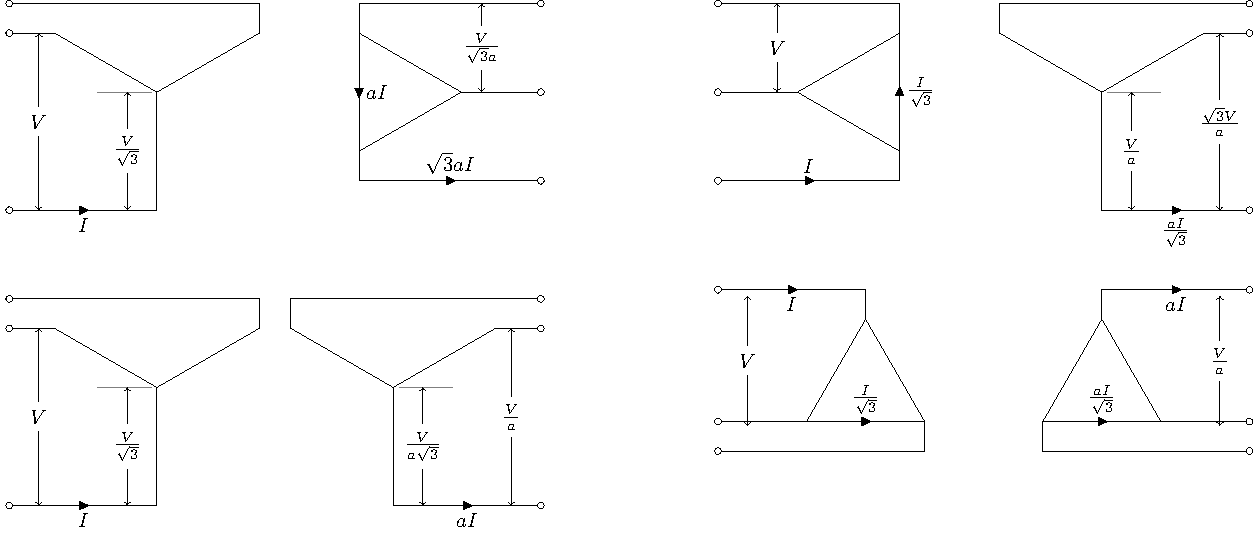
\includegraphics[width=\linewidth]{figTransformersAllPossibleConnections}
\caption{ابتدائی اور ثانوی جانب تار اور یک مرحلہ مقداروں کے رشتے۔}
\label{شکل_ٹرانسفارمر_تین_دور_ٹرانسفارمر_کے_مختلف_جوڑ}
\end{figure}


جیسے شکل \حوالہ{شکل_ٹرانسفارمر_تین_دور_ٹرانسفارمر_کے_مختلف_جوڑ} میں دکھایا گیا ہے ستارہ-تکونی ٹرانسفارمر کی تار پر برقی دباو کی نسبت
\begin{align}
\frac{V_\textup{{ابتدائی}}}{V_\textup{{ثانوی}}}=\sqrt{3} a =\sqrt{3} \left(\frac{N_1}{N_2} \right)
\end{align}
جبکہ ستارہ-ستارہ کا
\begin{align}
\frac{V_\textup{{ابتدائی}}}{V_\textup{{ثانوی}}}=a =\left(\frac{N_1}{N_2} \right)
\end{align}
تکونی-ستارہ کا
\begin{align}
\frac{V_\textup{{ابتدائی}}}{V_\textup{{ثانوی}}}=\frac{a}{\sqrt{3}}=\frac{1}{\sqrt{3}} \left(\frac{N_1}{N_2} \right)
\end{align}
اور تکونی-تکونی کا
\begin{align}
\frac{V_\textup{{ابتدائی}}}{V_\textup{{ثانوی}}}=a =\left(\frac{N_1}{N_2} \right)
\end{align}
ہے۔
%
\ابتدا{مثال}
یک مرحلہ  تین یکساں ٹرانسفارمروں کو ستارہ-تکونی \عددیء{Y:\Delta}  جوڑ کر تین مرحلہ ٹرانسفارمر بنایا گیا ہے۔ایک مرحلہ ٹرانسفارمر کی برقی \اصطلاح{سکت}\فرہنگ{سکت}\حاشیہب{rating}\فرہنگ{rating} درج ذیل ہے:
\begin{align*}
\SI{50}{\kilo \volt \ampere} , \quad 6350:440\,\textup{V}, \quad \SI{50}{\hertz}
\end{align*}
ستارہ-تکونی ٹرانسفارمر کی ابتدائی جانب \عددیء{11000}  وولٹ کی تین مرحلہ تار کی برقی دباو لاگو کیا گیا۔اس تین مرحلہ ٹرانسفارمر کی ثانوی جانب تار کا برقی دباو معلوم کریں۔

حل: حل کرتے وقت ہم ایک  عدد  یک مرحلہ ٹرانسفارمر پر نظر رکھیں گے۔ ابتدائی جانب اگر یک مرحلہ ٹرانسفارمر پر غور کیا جائے تو
\begin{align*}
\frac{N_1}{N_2}=\frac{V_1}{V_2}=\frac{6350}{440}
\end{align*}
اور اس پر لاگو برقی دباو مساوات \حوالہ{مساوات_ستارہ_ٹرانسفارمر_تار_اور_دور_رشتے}  کی مدد سے
\begin{align*}
V_{\textup{ابتدائی، یکمرحلہ}}=\frac{V_{\textup{تار}}}{\sqrt{3}}=\frac{11000}{\sqrt{3}}=\SI{6350.85}{\volt}
\end{align*}
ہے لہٰذا اس یک مرحلہ ٹرانسفارمر کی ثانوی جانب مساوات \حوالہ{مساوات_ٹرانسفارمر_تبادلہ_دباو_رو} کی مدد سے
\begin{align*}
V_{\textup{ثانوی}}=\frac{N_2}{N_1} V_{\textup{ابتدائی}}=\frac{440}{6350} \times 6350.85 \approx \SI{440}{\volt}
\end{align*}
ہیں۔چونکہ ثانوی جانب ان تین یک مرحلہ ٹرانسفارمروں کو تکونی جوڑا گیا ہے لہٰذا مساوات \حوالہ{مساوات_تکونی_ٹرانسفارمر_تار_اور_دور_رشتے}  کی مدد سے اس جانب تار کی برقی دباو یہی ہو گی۔اس تین مرحلہ ٹرانسفارمر کی تار پر برقی دباو کی نسبت
\begin{align*}
\frac{V_{\textup{ابتدائی، تار}}}{V_{\textup{ثانوی، تار}}}=\frac{11000}{440}
\end{align*}
ہے۔چونکہ یک مرحلہ ٹرانسفارمر \عددیء{50}  کلو وولٹ-ایمپیئر کا ہے لہٰذا یہ تین مرحلہ ٹرانسفارمر  \عددیء{150} کلو وولٹ-ایمپیئر کا ہو گا۔یوں اس تین مرحلہ ٹرانسفارمر کی سکت\فرہنگ{سکت}\حاشیہب{rating}\فرہنگ{rating}
\begin{align*}
\SI{150}{\kilo \volt \ampere}, \quad 11000:440\,\textup{V},\quad \SI{50}{\hertz}
\end{align*}
ہو گی۔

	ٹرانسفارمر پر لگی تختی\فرہنگ{تختی}\حاشیہب{name plate}\فرہنگ{name plate} پر اس کی سکت بیان ہوتی ہے جس میں ٹرانسفارمر کے دونوں جانب تار کے برقی دباو لکھے جاتے ہیں نہ کہ لچھوں کے چکر۔
\انتہا{مثال}
%
ستارہ-ستارہ جڑے ٹرانسفارمر عام طور استعمال نہیں ہوتے۔اس کی وجہ یہ ہے کہ اگرچہ ان کی تین مرحلہ برقی دباو  کے بنیادی جزو آپس میں \عددیء{120\degree}  زاویائی فاصلے پر ہوتے ہیں لیکن ان کی تیسری موسیقائی جزو آپس میں ہم قدم ہوتی ہیں۔قالب کی غیر بتدریج خصوصیات کی وجہ سے ٹرانسفارمر میں ہر صورت تیسری موسیقائی جزو پائے جاتے ہیں۔تیسری موسیقائی جزو ہم قدم ہونے کی وجہ سے جمع ہو کر ایک نہایت بڑی برقی دباو کی موج پیدا کرتے ہیں جو کبھی کبھی برقی دباو کی بنیادی جزو سے بھی زیادہ بڑھ جاتی ہے۔

بقایا تین قسم کے جڑے ٹرانسفارمروں میں برقی دباو کی تیسری موسیقائی جزو مسئلہ نہیں کرتیں چونکہ ان میں تکونی جُڑے لچھوں میں برقی رو گھومنے شروع ہو جاتی ہے جو ان کے اثر کو ختم کر دیتی ہے۔

تین مرحلہ ٹرانسفارمر کے متوازن دور حل کرتے وقت ہم تصور کرتے ہیں کہ ٹرانسفارمر ستارہ نما جڑا  ہے۔یوں اس کے ایک مرحلے میں برقی رو، تار  کی برقی رو ہی ہو گی اور اس کے ایک مرحلے پر لاگو برقی دباو، یک مرحلہ برقی دباو  ہو گا۔اسی طرح ہم تصور کرتے ہیں کہ اس پر لدا برقی بوجھ بھی ستارہ نما جُڑا ہے۔یوں تین مرحلہ کی جگہ ہم یک مرحلہ دور کا نسبتاً آسان مسئلہ حل کرتے ہیں۔ ایسا کرنے سے مسئلہ پر غور کرنا آسان ہو جاتا ہے۔یہ ایک مثال سے زیادہ بہتر سمجھ آئے گا۔
%
\ابتدا{مثال}
ایک تین مرحلہ \عددیء{\Delta :Y}   \عددیء{2000} کلو وولٹ-ایمپیئر،  \عددیء{11000:600 }  وولٹ اور \عددیء{50} ہرٹز پر چلنے والا کامل ٹرانسفارمر تین مرحلہ کے متوازن برقی بوجھ کو طاقت مہیا کر رہا ہے۔یہ بوجھ تکونی جڑا ہے جہاں بوجھ کا ہر حصہ \عددیء{(0.504+j0.1917)} کے برابر ہے۔شکل \حوالہ{شکل_ٹرانسفارمر_تکونی_بار_کی_مثال}  میں یہ دکھایا گیا ہے۔
\begin{itemize}
\item
اس شکل میں ہر جگہ برقی رو معلوم کریں۔
\item
برقی بوجھ\فرہنگ{بوجھ}\حاشیہب{electrical load}\فرہنگ{load} کو درکار طاقت معلوم کریں
\end{itemize}

\begin{figure}
\centering
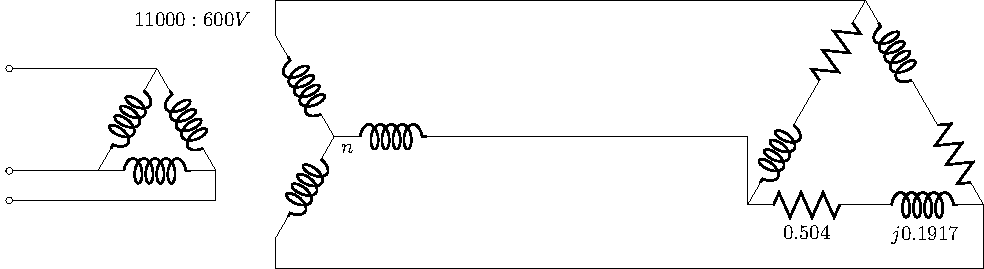
\includegraphics[width=\linewidth]{figTransformersDeltaLoadedExample}
\caption{ٹرانسفارمر تکونی متوازن بوجھ کو طاقت فراہم کر رہا ہے۔}
\label{شکل_ٹرانسفارمر_تکونی_بار_کی_مثال}
\end{figure}
حل:

پہلے تکونی بوجھ کو ستارہ نما بوجھ میں تبدیل کرتے ہیں
\begin{align*}
Z_Y= \frac{Z_\Delta}{3}=\frac{0.504+j0.1917}{3}=0.168+j0.0639
\end{align*}
اس بوجھ کو ستارہ نما جڑا شکل \حوالہ{شکل_ٹرانسفارمر_تکونی_بار_کو_ستارہ_تبادلہ} میں دکھایا گیا ہے۔اس شکل میں ایک برقی تار جسے نقطہ دار لکیر سے ظاہر کیا گیا ہے کو ٹرانسفارمر کی زمینی نقطہ سے بوجھ کے مشترکہ سرے کے درمیان جڑا دکھایا گیا ہے۔متوازن دور میں اس تار میں برقی رو صفر ہو گی۔حل کرنے کی نیت سے ہم اس متوازن دور سے ایک مرحلہ لے کر حل کرتے ہیں۔
\begin{figure}
\centering
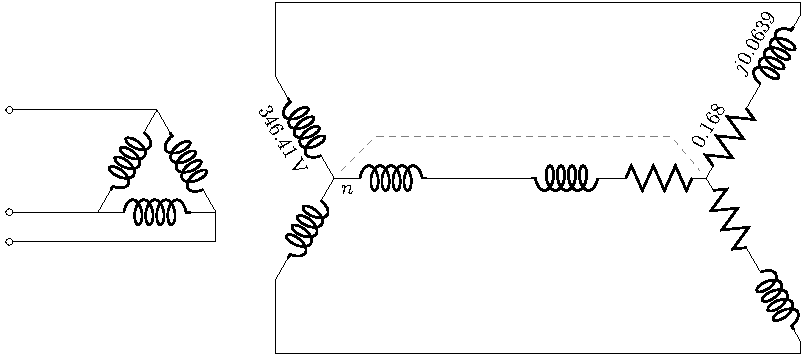
\includegraphics[width=\linewidth]{figTransformersDeltaLoadedExampleTurnedStar}
\caption{تکونی بوجھ کو مساوی ستارہ بوجھ میں تبدیل کیا گیا ہے۔}
\label{شکل_ٹرانسفارمر_تکونی_بار_کو_ستارہ_تبادلہ}
\end{figure}

یوں مساوی برقی بوجھ میں برقی رو
\begin{align*}
I=\frac{346.41}{0.168+j0.0639}=1927.262\phase{-20.825\degree}
\end{align*}
ہو گی اور اس ایک مرحلہ میں طاقت
\begin{align*}
p=346.41 \times 1927.262 \times \cos (-20.825\degree)=\SI{624007}{\watt}
\end{align*}
ہو گی۔ یوں برقی بوجھ کو پوری درکار برقی طاقت اس کے تین گنا ہو گی یعنی \عددیء{\SI{1872}{\kilo \watt}}  اس بوجھ کا جزو طاقت\حاشیہب{power factor} 
\begin{align*}
\cos (-20.825\degree)=0.93467
\end{align*}
ہے۔

	تکونی بوجھ   میں برقی رو \عددیء{\tfrac{1927.262}{\sqrt{3}}=1112.7} ایمپیئر ہو گی۔ ٹرانسفارمر کی ابتدائی جانب برقی تاروں میں برقی رو
\begin{align*}
\left(\frac{600}{11000} \right) \times 1927.262=105.12
\end{align*}
  ایمپیئر ہو گی۔
\انتہا{مثال}
%
اس مثال میں جزو طاقت \عددیء{0.93467} ہے۔اس کتاب کے لکھتے وقت پاکستان میں اگر صنعتی کارخانوں کی برقی بوجھ کی جزو طاقت \عددیء{0.9} سے کم ہو جائے تو برقی طاقت فراہم کرنے والا ادارہ (واپڈا) جرمانہ نافذ کرتا ہے۔ 

\حصہ{ٹرانسفارمر چالو کرتے لمحہ زیادہ محرکی برقی رو کا گزر}
ہم دیکھ چکے ہیں کہ اگر ٹرانسفارمر کے قالب میں کثافتِ مقناطیسی بہاو سائن نما ہو یعنی \عددیء{B=B_0 \sin \omega t}  تو اس کے لئے ہم لکھ سکتے ہیں
\begin{align*}
v=e=N \frac{\partial \varphi}{\partial t}&=N A_c \frac{\partial B}{\partial t}\\
&=\omega N A_c B_0 \cos \omega t\\
&=V_0 \cos \omega t
\end{align*}
یعنی
\begin{align}\label{مساوات_ٹرانسفارمر_درکار_کثافت_بہاو}
B_0=\frac{V_0}{\omega N A_c}
\end{align}
یہ مساوات برقرار چالو\فرہنگ{برقرار چالو}\حاشیہب{steady state} ٹرانسفارمر کے لئے درست ہے۔

تصور کریں کہ ایک ٹرانسفارمر کو چالو کیا جا رہا ہے۔ چالو ہونے سے پہلے قالب میں مقناطیسی بہاو صفر ہے اور جس لمحہ اسے چالو کیا جائے اس لمحہ بھی یہ صفر ہی رہتا ہے۔	

جس لمحہ ٹرانسفارمر کو چالو کیا جائے اس لمحہ لاگو برقی دباو
\begin{align*}
v=V_0 \cos (\omega t+\theta)
\end{align*}
ہے۔اگر \عددیء{\theta=\pi/2} یہ لمحہ ہو تو آدھے \اصطلاح{دوری عرصہ}\فرہنگ{دوری عرصہ}\حاشیہب{time period}\فرہنگ{time period}  کے بعد قالب میں کثافتِ مقناطیسی بہاو
\begin{align*}
B&=\frac{1}{N A_c} \int_{0}^{\pi/\omega} V_0 \cos (\omega t+\pi/2) \dif t\\
&=\frac{V_0}{\omega N A_c} \sin (\omega t+\pi/2)_0^{\pi/\omega}\\
&=-\left(\frac{2 V_0}{\omega N A_c} \right)
\end{align*}
یعنی کثافتِ مقناطیسی بہاو کا طول معمول سے دگنا ہو گا۔اگر یہی حساب \عددیء{\theta=0} لمحہ کے لئے کیا جائے تو زیادہ سے زیادہ کثافتِ مقناطیسی بہاو بالکل مساوات \حوالہ{مساوات_ٹرانسفارمر_درکار_کثافت_بہاو}  کے عین مطابق ہو گا۔ ان دو زاویوں کے مابین زیادہ سے زیادہ کثافتِ مقناطیسی بہاو ان دو حدوں کے درمیان رہتا ہے۔ 

قالب کی  \عددیء{B-H} خط غیر بتدریج بڑھتا ہے۔لہٰذا \عددیء{B}  دگنا کرنے کی خاطر \عددیء{H} کو کئی گنا بڑھانا ہو گا جو لچھے میں محرک برقی رو بڑھانے سے ہوتا ہے\حاشیہد{\عددیء{2000}  کلو وولٹ-ایمپیئر ٹرانسفارمر سے چالو کرتے وقت تھرتھراہٹ کی آواز آتی ہے}۔یہاں صفحہ \حوالہصفحہ{شکل_مقناطیسی_ادوار_ہیجان_رو_چال_نظرانداز} پر دکھائے  شکل \حوالہ{شکل_مقناطیسی_ادوار_ہیجان_رو_چال_نظرانداز}  سے رجوع کریں۔قوی ٹرانسفارمروں میں ہیجانی کثافتِ مقناطیسی بہاو کی چوٹی \عددیء{1\le B_0\le 1.3} ہوتی ہے۔ٹرانسفارمر چالو کرتے لمحہ یوں کثافتِ مقناطیسی بہاو  \عددیء{2} سے  \عددیء{2.6} ٹسلا تک ہو سکتی ہے جس کے لئے درکار ہیجان انگیز برقی رو نہایت زیادہ ہو گی۔


\باب{برقی اور میکانی توانائی کا باہمی تبادلہ}
برقی رو یا مقناطیسی بہاو کی مدد سے برقی توانائی کو میکانی توانائی یا میکانی توانائی کو برقی توانائی میں تبدیل کیا جاتا ہے۔ مختلف مشین میں یہ عمل ہوتا ہے۔ ناپنے کے مشین نہایت کم طاقت کا تبادلہ کرتے ہیں۔ ان میں لاؤڈ سپیکر، مائکروفون وغیرہ شامل ہیں۔ ان کے برعکس ایک اور قسم کے مشین قوت پیدا کرتے ہیں۔ ان میں برقی مقناطیس، رِیلے\فرہنگ{رِیلے}\حاشیہب{relay}\فرہنگ{relay}  وغیرہ شامل ہیں۔ ایک تیسری قسم، جن میں برقی موٹر اور جنریٹر شامل ہیں، لگاتار توانائی کو ایک شکل سے دوسری شکل میں تبدیل کرتے ہیں۔

اس باب میں مقناطیسی بہاو کی مدد سے توانائی کے تبادلہ پر غور کیا جائے گا۔برقی رو کی مدد سے توانائی کے تبادلہ کو انہیں طرح کے طریقوں سے حل کیا جاتا ہے اگرچہ ان کا تذکرہ اس کتاب میں نہیں کیا جائے گا۔

 اس باب میں جو تراکیب ہم سیکھیں گے وہ بہت اہمیت رکھتے ہیں اور انجنیئرنگ میں بہت سے مسائل حل کرنے میں مدد گار ثابت ہوتے ہیں۔

\حصہ{مقناطیسی نظام میں قوت  اور  قوت گردشہ}
اگر ایک برقی میدان میں برقی بار \عددیء{q} رکھا جائے تو اس پر قوت
\begin{align}
\kvec{F}=q \kvec{E}
\end{align}
پائی جاتی ہے۔اگر برقی بار مثبت ہو تو یہ قوت برقی شدت \سمتیہ{E} کی سمت میں ہوتی ہے اور اگر برقی بار منفی ہو تو یہ قوت \سمتیہ{E} کی الٹ سمت میں ہوتی ہے۔ اسی طرح اگر ایک برقی بار مقناطیسی میدان میں حرکت کر رہا ہو اور اس کی \اصطلاح{سمتی رفتار}\فرہنگ{سمتی رفتار}\حاشیہب{velocity} \سمتیہ{v} ہو تو اس پر قوت
\begin{align}\label{مساوات_برقی_میکانی_تبادلہ_مقناطیسی}
\kvec{F}=q \left(\kvec{v} \times \kvec{B} \right)
\end{align}
پائی جاتی ہے۔ اس مرتبہ مثبت برقی بار پر قوت کی سمت \اصطلاح{دائیں ہاتھ کے قانون}\حاشیہب{right hand rule} سے معلوم کی جاتی ہے۔ اگر دائیں ہاتھ کی چار انگلیاں \سمتیہ{v} کی سمت میں رکھ کر انہیں \سمتیہ{B} کی سمت میں موڑا جائے تو انگوٹھا \سمتیہ{F} کی سمت میں ہو گا۔ منفی برقی بار پر قوت اس کے مخالف سمت میں ہو گی۔یہاں سمتی رفتار \عددیء{q} اور \سمتیہ{B} کے مابین ہے۔ اگر ایک برقی بار بیک وقت مقناطیسی اور برقی میدان میں حرکت کر رہا ہو تب اس پر قوت ہمیں گزشتہ دو قوانین ملا کر یعنی مساوات \اصطلاح{لورینز}\فرہنگ{مساوات لورینز}\حاشیہب{Lorenz equation}\فرہنگ{Lorenz equation}  سے ملتی ہے۔
\begin{align}
\kvec{F}=q \left(\kvec{E}+\kvec{v} \times \kvec{B}  \right)
\end{align}
مساوات  \حوالہ{مساوات_برقی_میکانی_تبادلہ_مقناطیسی} میں اگر \عددیء{\kvec{v}=\dif \kvec{L} / \dif t} لی جائے تو اسے یوں لکھا جا سکتا ہے۔
\begin{gather}
\begin{aligned}
\kvec{F}&=q \left(\frac{\dif \kvec{L}}{\dif t} \times \kvec{B} \right)\\
&=\frac{q}{\dif t} \left(\dif \kvec{L} \times \kvec{B} \right)\\
&=i \left(\dif \kvec{L} \times \kvec{B}  \right)
\end{aligned}
\end{gather}
%
\ابتدا{مثال}
شکل \حوالہ{شکل_تبادلہ_طاقت_لچھے_پر_قوت_اور_مروڑ} میں ایک لچھا مقناطیسی میدان میں دکھایا گیا ہے۔لچھے کی رداس \عددیء{15} سم، محوری لمبائی \عددیء{50} سم اور اس میں برقی رو  \عددیء{5} ایمپیئر ہے۔کثافتِ مقناطیسی بہاو کو نقطہ دار نوک والی لکیروں سے شمالی قطب سے جنوبی قطب کی جانب دکھایا گیا ہے۔اگر کثافتِ مقناطیسی بہاو \عددیء{0.55} ٹیسلہ ہو تو 
\begin{itemize}
\item
لچھے کے اطراف پر قوت معلوم کریں اور
\item
لچھے پر قوت گردشہ \سمتیہ{\tau} معلوم کریں
\end{itemize}
%
\begin{figure}
\centering
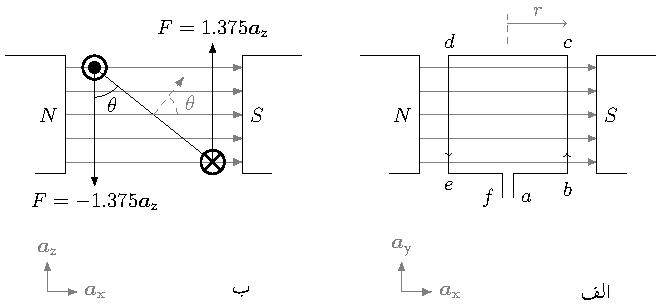
\includegraphics{figEnergyConversionTorqueOnOneTurn}
\caption{ایک چکر کے لچھے پر قوت اور قوت گردشہ}
\label{شکل_تبادلہ_طاقت_لچھے_پر_قوت_اور_مروڑ}
\end{figure}
%
حل:
	شکل-الف اور ب میں کارتیسی اکائی سمتیہ دیئے گئے ہیں۔اگر برقی تار کے سروں کو نظر انداز کیا جائے اور اسے ایک بند دائرہ سمجھا جائے تو  شکل-الف میں  برقی رو کی سمت میں تار کے اطراف کی لمبائیاں 
\begin{align*}
\kvec{L}_{bc}&=l \ay\\
\kvec{L}_{cd}&=-2 r \ax\\
\kvec{L}_{de}&=-l \ay\\
\kvec{L}_{eb}&=2 r \ax
\end{align*}
ہیں جبکہ \عددیء{\kvec{B}=B_0 \ax} ہے۔یوں مساوات \حوالہ{مساوات_برقی_میکانی_تبادلہ_مقناطیسی}  سے ان اطراف پر قوت
\begin{align*}
\kvec{F}_{bc}&= i \left(\kvec{L}_{bc} \times B_0 \ax \right)\\
&=5 \left(0.5 \ay \times 0.55 \ax \right)\\
&=-1.375 \az\\
\kvec{F}_{cd}&= 5\left(-0.3\ax \times 0.55 \ax \right)\\
&=0\\
\kvec{F}_{de}&= 5 \left(-0.5\ay \times 0.55 \ax \right)\\
&=1.375 \az\\
\kvec{F}_{ea}&= 0
\end{align*}
نیوٹن ہو گی۔ہم دیکھتے ہیں کہ قوت محوری لمبائی کی جانب اطراف پر ہی لاگو  ہے۔یہ دو قوت حصہ با میں دکھائے گئے ہیں جہاں سے یہ واضح ہے کہ یہ قوت گردشہ پیدا کریں گی۔ اس قوت گردشہ کی سمت دائیں ہاتھ کے قانون سے بھی با آسانی معلوم کی جا سکتی ہے۔قوت گردشہ
\begin{align*}
\kvec{\tau}&=-1.375 \times 2 \times 0.15 \times \sin \theta \ay\\
&=-0.4125 \sin \theta \ay
\end{align*}
نیوٹن-میٹر ہے۔
\انتہا{مثال}
%
	 ان مساوات کا استعمال صرف سادہ ترین جگہوں ممکن ہوتا ہے۔ استعمال میں آنے والی مشین میں ان مساوات سے قوت کا تعین کرنا نہایت مشکل ثابت ہوتا ہے۔ اب ہم وہ طریقہ سیکھتے ہیں جس کی مدد سے ہم مختلف مشین میں قوت کا تعین کر سکیں گے۔ اس طریقہ کو توانائی کا طریقہ کہتے ہیں اور یہ توانائی کے اٹل ہونے پر مبنی ہے۔

گھومتی برقی مشین میں عموماً دو لچھے ہوتے ہیں۔ ان میں ایک لچھا  مشین کے ساکن حصہ پہ لپٹا ہوتا ہے اور اسی لئے ساکن رہتا ہے۔ لہٰذا  اس کو \اصطلاح{ساکن لچھا}\فرہنگ{ساکن لچھا}\فرہنگ{لچھا! ساکن}\حاشیہب{stator coil}\فرہنگ{stator coil}   کہتے ہیں ۔  دوسرا لچھا  مشین کے گھومنے والے حصہ پہ لپٹا ہوتا ہے اور مشین گھومنے سے یہ بھی گھومتا ہے۔ لہٰذا اس کو \اصطلاح{گھومتا لچھا}\فرہنگ{گھومتا لچھا}\فرہنگ{لچھا!گھومتا}\حاشیہب{rotor coil}\فرہنگ{rotor coli}  کہتے ہیں۔  ایسے مشین  کو اس طرح سمجھنا نہایت آسان ہے کہ ہم ان دو لچھوں کو دو مقناطیس سمجھیں۔ جس طرح دو مقناطیس اگر قریب لائے جائیں تو یہ کوشش کرتے ہیں کہ ایک کا شمال \عددیء{N} دوسرے کے جنوب \عددیء{S} کی سمت  ہو۔

 موٹر میں دونوں  لچھے مقناطیس پیدا کرتے ہیں۔ ساکن لچھے کا مقناطیسی بہاو،  گھومتے لچھے کے مقناطیسی بہاو سے کچھ آگے رہتا ہے اور  اسے کھینچتا رہتا ہے۔ ایسا کرنے سے یہ کام کرتا ہے۔ جنریٹر میں اس کے برعکس  گھومتا لچھا، ساکن لچھے پر کام کرتے ہوئے اس میں برقی دباؤ پیدا کرتا ہے۔

توانائی کے طریقے کو شکل \حوالہ{شکل_تبادلہ_توانائی_نظام_بطور_ڈبہ}  کی مدد سے سمجھا جا سکتا ہے۔یہاں مقناطیسی نظام کو ایک ڈبہ کی شکل میں دکھایا گیا ہے۔ اس کو برقی توانائی مہیا کی جاتی ہے جس سے یہ میکانی توانائی پیدا کرتا ہے۔ یہاں برقی توانائی کے دو متغیرہ  \عددیء{e} اور \عددیء{i} ہیں اور میکانی توانائی کے متغیرہ فاصلہ \عددیء{x} اور میدانی قوت\حاشیہد{میدانی قوت \عددیء{F_m} میں چھوٹی لکھائیی میں \عددیء{m} لفظ میدانی کو ظاہر کر رہا ہے۔} \عددیء{F_m} ہیں۔ اس شکل میں بائیں جانب یعنی ابتدائی یا اولین جانب \عددیء{i} کا رُخ باہر سے اندر کی طرف ہے اور دائیں جانب یعنی ثانوی جانب \عددیء{F_m} کا رُخ اندر سے  باہر کی جانب ہے۔یہ  ٹرانسفارمر دور کے شکل \حوالہ{شکل_ٹرانسفارمر_کامل_بار_بردار_ٹرانسفارمر}  کی مانند ہے۔

اگر نظام میں توانائی کی ضیاع کو توانائی کے ذخیرہ ہونے سے علیحدہ کرنا ممکن ہو تو ایسی صورت میں توانائی کے ضیاع  کو بیرونی رکن سے پیش کیا جاتا ہے۔ شکل \حوالہ{شکل_تبادلہ_توانائی_قوت_پیدا_کرتا_آلا}   میں ایک ایسا ہی نظام دکھایا گیا ہے جس میں  لچھا برقی نظام کو پیش کرتا ہے اور حرکت کرنے والا حصہ میکانی نظام کو پیش کرتا ہے۔ یہاں لچھے میں توانائی کے ضیاع کو، بیرونی  مزاحمت \عددیء{R} سے ظاہر کیا گیا ہے۔
\begin{figure}
\centering
\includegraphics{figEnergyConversionBasicBlockDiagram}
\caption{ برقی توانائی سے میکانی توانائی کے تبادلہ کا نظام۔}
\label{شکل_تبادلہ_توانائی_نظام_بطور_ڈبہ}
\end{figure}
%
\begin{figure}
\centering
\includegraphics{figEnergyConversionForceGeneratingDevice}
\caption{ قوت پیدا کرنے والا آلا۔}
\label{شکل_تبادلہ_توانائی_قوت_پیدا_کرتا_آلا}
\end{figure}

توانائی کا بنیادی اصول کہتا ہے کہ توانائی نا تو پیدا کی جا سکتی ہے اور نا ہی اسے تباہ کیا جا سکتا ہے۔ اس کو صرف ایک قسم  سے دوسرے قسم کی توانائی میں تبدیل کیا جا سکتا ہے۔ لہٰذا اسے جو برقی توانائی \عددیء{\partial W_{\textup{برقی}}} دی جائے  اس میں سے کچھ میکانی توانائی \عددیء{\partial W_{\textup{میکانی}}}  میں تبدیل ہو گی، کچھ  مقناطیسی میدان میں  ذخیرہ ہو گی یعنی \عددیء{\partial W_{\textup{مقناطیسی}}} اور بقایا مختلف طریقوں سے  ضائع \عددیء{\partial W_{\textup{ضائع}}} ہو گی  جو ہمارے کسی کام نہ آ سکے گی۔ یعنی
\begin{align}
\partial W_{\textup{برقی}}=\partial W_{\textup{میکانی}}+\partial W_{\textup{مقناطیسی}}+\partial W_{\textup{ضائع}}
\end{align}
اگر برقی توانائی کے ضیاع کو نظرانداز کیا جائے تو
\begin{align}
\partial W_{\textup{برقی}}=\partial W_{\textup{میکانی}}+\partial W_{\textup{مقناطیسی}}
\end{align}
اس مساوات کو \عددیء{\partial t} سے تقسیم کرنے سے حاصل ہوتا ہے

\begin{align}
\frac{\partial W_{\textup{برقی}}}{\partial t}=\frac{\partial W_{\textup{میکانی}}}{\partial t}+\frac{\partial W_{\textup{مقناطیسی}}}{\partial t}
\end{align}
یہ مساوات توانائی کی بجائے طاقت کی بات کرتا ہے۔ اگر ہم بائیں ہاتھ کی جانب یعنی برقی طاقت کو \عددیء{e i} لکھیں اور  دائیں ہاتھ کی جانب   میکانی حصہ میں \عددیء{\partial W_{\textup{میکانی}}=F_m \partial x} لکھیں تو
\begin{align}
e i = F_m \frac{\partial x}{\partial t} +\frac{\partial W_m}{\partial t}
\end{align}
حاصل ہوتا ہے جہاں \عددیء{W_{\textup{مقناطیسی}}}  کو \عددیء{W_m} لکھا گیا ہے۔مساوات \حوالہ{مساوات_مقناطیسی_دور_فیراڈے_قانون}   کے استعمال سے اسے یوں لکھا جا سکتا ہے۔
\begin{align}
i \frac{\partial \lambda}{\partial t}=F_m \frac{\partial x}{\partial t}+\frac{\partial W_m}{\partial t}
\end{align}
یا
\begin{align}\label{مساوات_برقی_مقناطیسی_تبادلہ_توانائی_کا_طریقہ}
\partial W_m=i \partial \lambda-F_m \partial x
\end{align}
مساوات \حوالہ{مساوات_برقی_مقناطیسی_تبادلہ_توانائی_کا_طریقہ} توانائی کے طریقہ کی بنیاد ہے۔ یہ مساوات استعمال کرتے وقت یاد رہے کہ قوت بنیادی طور پر لورینز کے قانون\حاشیہب{Lorenz equation} سے ہی پیدا ہوتی ہے۔مساوات \حوالہ{مساوات_برقی_مقناطیسی_تبادلہ_توانائی_کا_طریقہ}  میں برقی متغیرہ \عددیء{i} اور \عددیء{e} کی بجائے \عددیء{i} اور \عددیء{\lambda} ہیں۔ لہٰذا شکل \حوالہ{شکل_تبادلہ_توانائی_نظام_بطور_ڈبہ}    کو شکل \حوالہ{شکل_تبادلہ_توانائی_قوت_پیدا_کرتا_آلا_زیادہ_معلومات}   کی طرح بھی بنایا جا سکتا ہے۔
\begin{figure}
\centering
\includegraphics{figEnergyConversionBasicBlockDiagramDetailed}
\caption{توانائی کی شکل تبدیل کرنے والا ایک نظام۔}
\label{شکل_تبادلہ_توانائی_قوت_پیدا_کرتا_آلا_زیادہ_معلومات}
\end{figure}

	کسی بھی تفاعل\حاشیہب{function} \عددیء{z(x,y)} کے لئے ہم لکھ سکتے ہیں
\begin{align}\label{مساوات_تبادلہ_جزوی_تفرق_عمومی_الف}
\partial z(x,y)=\frac{\partial z}{\partial x} \dif x+\frac{\partial z}{\partial y} \dif y
\end{align}
اسی طرح ہم \عددیء{W_m(x,\lambda)} کے لئے لکھ سکتے ہیں۔
\begin{align}\label{مساوات_تبادلہ_جزوی_تفرق_عمومی_ب}
\partial W_m(x,\lambda)=\frac{\partial W_m}{\partial x}\dif x+\frac{\partial W_m}{\partial \lambda}\dif \lambda
\end{align}
اس مساوات اور مساوات \حوالہ{مساوات_برقی_مقناطیسی_تبادلہ_توانائی_کا_طریقہ} سے ہم اخذ کر سکتے ہیں کہ
\begin{align}
F_m(x,\lambda)&=-\left. \frac{\partial W_m(x,\lambda)}{\partial t}\right|_{\lambda_0}\label{مساوات_تبادلہ_توانائی_قوت_برقی_رو}\\
i(x,\lambda)&=\left. \frac{\partial W_m(x,\lambda)}{\partial \lambda}\right|_{x_0}\label{مساوات_تبادلہ_توانائی_سے_رو}
\end{align}
اگر ہم مقناطیسی میدان میں مقناطیسی توانائی \عددیء{W_m(x,\lambda)} معلوم کر سکیں تو مساوات \حوالہ{مساوات_تبادلہ_توانائی_قوت_برقی_رو}  کو استعمال کر کے ہم قوت کا حساب لگا سکتے ہیں۔ ہم اگلے حصہ میں یہی کرتے ہیں۔

\حصہ{تبادلہ توانائی والا ایک لچھے کا نظام}
شکل \حوالہ{شکل_تبادلہ_توانائی_قوت_پیدا_کرتا_آلا}  میں  ایک لچھے کا سادہ نظام دکھایا گیا ہے۔ لچھے میں برقی ضیاع کو بیرونی مزاحمت سے پیش کیا گیا ہے۔ میکانی نظام میں حرکت کرنے والے حصہ کے کمیت کو نظرانداز کیا گیا ہے۔ اگر اس کمیت  کے اثر کا بھی حساب لگانا ہو تو اس کمیت کو ایک بیرونی کمیت تصور کیا جا سکتا ہے۔ اس طرح تبادلہ توانائی کے نظام پر غور کرنا آسان ہو جاتا ہے۔ 

قوت پیدا کرنے والے مشین میں حرکت ناگزیر ہے۔عموماً حرکت تب ممکن ہوتی ہے جب مقناطیسی قالب میں خلاء ہو جو کم اور زیادہ ہو سکے۔  عموماً \عددیء{\Re_a \gg \Re_c} ہوتا ہے۔لہٰذا جب بھی خلائی درز رکنے والی  مقناطیسی دور حل کرنی ہو،  ہم \عددیء{\Re_c} کو نظرانداز کر سکتے ہیں۔ایسا کرنے سے، جیسا مساوات \حوالہ{مساوات_مقناطیسی_ڈور_بہاو_مساوی_دباؤ_بٹا_ہچکچاہٹ}  میں دیا گیا ہے، ہم  مقناطیسی دباؤ \عددیء{\tau} اور مقناطیسی بہاو \عددیء{\phi} کو براہ راست متناسب لکھ سکتے ہیں۔ اسی طرح مساوات \حوالہ{مساوات_مقناطیسی_دور_خود_امالہ_تعریف}   کو اب  ہم  یوں لکھ سکتے ہیں
\begin{align}\label{مساوات_تبادلہ_ارتباط_بہاو_اور_امالہ}
\lambda=L(x) i
\end{align}
اس مساوات میں امالہ  کو \عددیء{L(x)} لکھ کر اس بات کی نشاندہی کی گئی ہے کہ یہ صرف اور صرف  شکل \حوالہ{شکل_تبادلہ_توانائی_قوت_پیدا_کرتا_آلا}   میں خلاء کی لمبائی \عددیء{x} پر منحصر ہے۔

شکل \حوالہ{شکل_تبادلہ_توانائی_قوت_پیدا_کرتا_آلا}  میں قوت \عددیء{F_m}  کی سمت میں طے ہونے والا فاصلہ \عددیء{x} ہے۔ یوں  میکانی کام \عددیء{\partial W_{\textup{میکانی}}=F_m \dif x} کے برابر ہو گا جبکہ  \عددیء{\partial W_{\textup{برقی}}=i \dif \lambda}۔ یوں شکل \حوالہ{شکل_تبادلہ_توانائی_قوت_پیدا_کرتا_آلا}   کو مساوات \حوالہ{مساوات_برقی_مقناطیسی_تبادلہ_توانائی_کا_طریقہ}  ظاہر کرتی ہے۔ اگر ہمیں مقناطیسی میدان میں ذخیرہ توانائی \عددیء{W_m} معلوم کرنی ہو تو ہمیں مساوات \حوالہ{مساوات_برقی_مقناطیسی_تبادلہ_توانائی_کا_طریقہ}  کا تکمل\حاشیہب{integral}  لینا ہو گا۔ یعنی
\begin{align}\label{مساوات_تبادلہ_توانائی_تکمل}
\int \partial W_m = \int i(x,\lambda) \dif \lambda-\int F_m(x,\lambda) \dif x
\end{align}
اس تکمل کا حصول شکل \حوالہ{شکل_تبادلہ_توانائی_مقناطیسی_میدان_میں_توانائی}   سے واضح ہو گا۔ابتدائی نقطے پر مقناطیسی نظام کو کوئی برقی توانائی نہیں دی گئی۔ اس لئے اس میں  برقی رو صفر ہے۔ برقی رو صفر ہونے کی وجہ سے  مقناطیسی بہاو اور  ارتباط بہاو بھی صفر ہے۔اسی وجہ سے مقناطیسی میدان میں مقناطیسی توانائی بھی صفر ہے۔یوں  قوت اور حرکت بھی صفر ہے۔ یعنی ابتدائی نقطہ پر
\begin{align*}
i=\phi=\lambda=W_m=F_m=x=0
\end{align*}
ہے۔ابتدائی نقطہ شکل \حوالہ{شکل_تبادلہ_توانائی_مقناطیسی_میدان_میں_توانائی}  میں دکھایا گیا ہے۔ ہم اب لچھے کو برقی توانائی فراہم کرتے ہیں۔ لچھے میں برقی رو رواں ہوتی ہے جس سے قوت اور حرکت پیدا ہوتی ہے۔ ہم آخر کار  اختتامی نقطے پہ پہنچ جاتے ہیں۔اختتامی نقطہ بھی شکل میں دکھایا گیا ہے۔ اس نقطہ پہ \عددیء{\lambda=\lambda_0} اور \عددیء{x=x_0} ہے اور یہاں مقناطیسی میدان میں توانائی \عددیء{W_m(x_0,\lambda_0)} ہے۔ہم ابتدائی نقطہ  سے اختتامی نقطہ  تک پہنچنے کے لئے  برقی توانائی کو یوں بڑھاتے ہیں کہ \عددیء{\lambda} اور \عددیء{x}  شکل \حوالہ{شکل_تبادلہ_توانائی_مقناطیسی_میدان_میں_توانائی}  میں موٹی لکیر سے دکھائے اصل راستے پر رہیں۔لہٰذا ہمیں آخری نقطہ پہ مقناطیسی میدان میں مقناطیسی توانائی \عددیء{W_m(x_0,\lambda_0)} معلوم کرنے کے لئے مساوات \حوالہ{مساوات_تبادلہ_توانائی_تکمل}  کا اصل راستے پہ تکمل کرنا ہو گا۔ ایسا کرنا خاصا مشکل کام ہے۔ بجائے یہ ہم ایک بہتر راستہ اختیار کرتے ہیں۔
\begin{figure}
\centering
\includegraphics{figEnergyConversionEnergyInMagneticField}
\caption{مقناطیسی میدان میں توانائی۔}
\label{شکل_تبادلہ_توانائی_مقناطیسی_میدان_میں_توانائی}
\end{figure}


ہم اس حقیقت سے فائدہ اٹھاتے ہیں کہ مقناطیسی میدان ایک \اصطلاح{قدامت پسند میدان}\فرہنگ{قدامت پسند میدان}\حاشیہب{conservative field}\فرہنگ{conservative field}   ہے جس کا مطلب ہے کہ مقناطیسی میدان میں مقناطیسی توانائی صرف اور صرف اختتامی نقطہ کے \عددیء{x_0} اور \عددیء{\lambda_0} کی مقدار پر منحصر ہے\حاشیہد{تجاذبی میدان بھی قدامت پسند میدان ہے اسی لئے اگر کمیت \عددیء{m} کو کسی بھی راستے \عددیء{h} کی بلندی تک لے جایا جائے تو اس کی توانائی \عددیء{mgh} ہو گی۔}۔ اس کا مطلب یہ ہے کہ ہم جس راستے سے بھی آخری نقطہ تک پہنچیں ہمیں مقناطیسی میدان میں مقناطیسی توانائی یکساں ملے گی۔ لہٰذا ہم تکمل کرتے وقت شکل  \حوالہ{شکل_تبادلہ_توانائی_مقناطیسی_میدان_میں_توانائی} میں ابتدائی نقطہ سے  پہلے راستے چلتے ہیں اور جب ہم  فاصلہ  \عددیء{x_0} طے کر لیں تو یہاں سے دوسرا راستہ اختیار کر کے اختتامی نقطہ \عددیء{(x_0,\lambda_0)} پہ پہنچتے ہیں۔ لہٰذا ہم مساوات \حوالہ{مساوات_تبادلہ_توانائی_تکمل}   کو اب دو ٹکڑوں میں لکھیں گے، نقطہ \عددیء{(0,0)} سے نقطہ  \عددیء{(x_0,0)} تک اور پھر یہاں سے نقطہ \عددیء{(x_0,\lambda_0)}  تک
\begin{align}\label{مساوات_تبادلہ_توانائی_تکمل_راستہ_دو_ٹکڑے}
\int\limits_{\textup{اصل راستہ}} \partial W_m =\int\limits_{\textup{پہلا راستہ}} \partial W_m +\int\limits_{\textup{دوسرا راستہ}} \partial W_m 
\end{align}
اس مساوات کی دائیں جانب جزو کو باری باری دیکھتے ہیں۔پہلے راستے تکمل کو یوں لکھا جا سکتا ہے۔
\begin{align}\label{مساوات_تبادلہ_توانائی_تکمل_پہلا_راستہ}
\int\limits_{\textup{پہلا راستہ}} \partial W_m =\int_0^0 i(x,0) \dif \lambda-\int_0^{x_0} F_m(x,0) \dif x
\end{align}
	اس  راستے جیسے شکل \حوالہ{شکل_تبادلہ_توانائی_مقناطیسی_میدان_میں_توانائی}  سے ظاہر ہے اگر ہم \عددیء{x=0} سے  \عددیء{x=x_0} تک چلیں تو اس پورے راستے پر \عددیء{\lambda} صفر کے برابر ہی رہتا ہے۔ مساوات \حوالہ{مساوات_تبادلہ_توانائی_تکمل_پہلا_راستہ}  میں اس بات کو برقی رو \عددیء{i(x,0)}  اور قوت \عددیء{F_m(x,0)}  لکھ کر واضح کیا گیا ہے۔ چونکہ \عددیء{\lambda} کے شروع اور آخری مقدار  برابر ہیں لہٰذا اس مساوات میں \عددیء{\int_0^0 i(x,0)\dif \lambda =0} ہے۔

 اگر \عددیء{\lambda=0} ہو تو مقناطیسی بہاو بھی صفر ہو گا۔ مقناطیسی بہاو کے صفر ہونے کا مطلب ہے کہ کوئی مقناطیسی اثر موجود نہیں لہٰذا قوت \عددیء{F_m} بھی صفر ہو گا۔ اور ہم جانتے ہیں کہ صفر کا تکمل صفر ہی ہوتا ہے۔ لہٰذا اس مساوات میں \عددیء{\int_0^{x_0} F_m(x,0)\dif x=0} ہو گا۔ یوں پہلے راستے پر تکمل یعنی مساوات \حوالہ{مساوات_تبادلہ_توانائی_تکمل_پہلا_راستہ}  صفر کے برابر ہے یعنی
\begin{align}
\int\limits_{\textup{پہلا راستہ}} \partial W_m =\int_0^0 i(x,0) \dif \lambda-\int_0^{x_0} F_m(x,0) \dif x=0
\end{align}
اسی طرح مساوات \حوالہ{مساوات_تبادلہ_توانائی_تکمل_راستہ_دو_ٹکڑے} کی دوسرے راستے کے تکمل کے جزو کو یوں لکھا جا سکتا ہے۔
\begin{align}
\int\limits_{\textup{دوسرا راستہ}} \partial W_m =\int_0^{\lambda_0} i(x_0,\lambda) \dif \lambda-\int_{x_0}^{x_0} F_m(x_0,\lambda) \dif x
\end{align}
اس میں ہم دیکھتے ہیں کہ پورے راستے \عددیء{x=x_0} رہتا ہے۔ قوت کا تکمل صفر ہے چونکہ  \عددیء{x} کے  ابتدائی اور اختتامی قیمتیں برابر ہیں۔  یعنی
\begin{align}
\int_{x_0}^{x_0} F_m(x_0,\lambda) \dif x=0
\end{align}
آخر میں رہ گیا برقی رو کا تکمل۔ مساوات \حوالہ{مساوات_تبادلہ_ارتباط_بہاو_اور_امالہ}  کو استعمال کرتے ہوئے
\begin{align}
\int_0^{\lambda_0} i(x_0,\lambda) \dif \lambda=\frac{1}{L(x_0)} \int_0^{\lambda_0} \lambda \dif \lambda=\frac{\lambda_0^2}{2 L(x_0)}
\end{align}
اس طرح ہمیں آخر کار مقناطیسی میدان میں توانائی کی مساوات حاصل ہو گئی۔
\begin{align}
W=\frac{\lambda_0^2}{2 L(x_0)}
\end{align}

اس مساوات کی مدد سے مساوات \حوالہ{مساوات_تبادلہ_توانائی_قوت_برقی_رو}  کے ذریعہ قوت  \عددیء{F_m(x,\lambda)} اور مساوات \حوالہ{مساوات_تبادلہ_توانائی_سے_رو}  کے ذریعہ برقی رو \عددیء{i(x,\lambda)}  کا حساب اب ممکن ہے۔
%
\ابتدا{مثال}\شناخت{مثال_تبادلہ_توانائی_درز_میں_مقناطیسی_توانائی}
شکل \حوالہ{شکل_تبادلہ_توانائی_حرکت_اور_توانائی}  میں حرکت کرنے والا ایک مقناطیسی نظام دکھایا گیا ہے۔ حرکت کرنے والے حصے اور ساکن حصے  کے مابین خلائی درز \عددیء{g} ہے۔ اگر \عددیء{N=500} ،\عددیء{g=\SI{1}{\milli \meter}} ،\عددیء{b=\SI{0.2}{\meter}}، \عددیء{w=\SI{0.4}{\meter}} اور \عددیء{i=\SI{30}{\ampere}} ہوں تو اس خلائی درز میں توانائی \عددیء{W_m} معلوم کریں۔
\begin{figure}
\centering
\includegraphics{figEnergyConversionForceOnPlunger}
\caption{حرکت اور توانائی۔}
\label{شکل_تبادلہ_توانائی_حرکت_اور_توانائی}
\end{figure}

حل:
چونکہ \عددیء{h \gg g} ہے لہٰذا مقناطیسی بہاو کا بیشتر حصہ حرکت کرتے حصے سے گزرے گا۔ساکن حصے میں مقناطیسی بہاو خلائی درز کے قریب مڑ کر حرکت کرتے حصے میں سے گزرے گا۔ہمیں معلوم ہے کہ \عددیء{W_m=\tfrac{\lambda^2}{2L}}  اور \عددیء{L=\lambda i} ہیں لہٰذا \عددیء{W_m=\tfrac{1}{2} L i^2} لکھا جا سکتا ہے جہاں \عددیء{L=\tfrac{N^2 \mu_0 A_g}{2 g}} اور \عددیء{A_g=w(b-x)} کے برابر ہیں۔یوں
\begin{align*}
W_m&=\frac{1}{2} \frac{N^2 \mu_0 A_g}{2 g } i^2\\
&=\frac{1}{2} \times \frac{500^2 \times 4 \pi 10^{-7} \times 0.4 (0.2-x)}{2 \times 0.001} \times 30^2\\
&=28278 (0.2-x)
\end{align*}
جاول کے برابر ہے۔
\انتہا{مثال}
%
\ابتدا{مثال}\شناخت{مثال_تبادلہ_توانائی_قوت_کا_حصول_بذریعہ_توانائی_طریقہ}
 شکل \حوالہ{شکل_تبادلہ_توانائی_حرکت_اور_توانائی} میں توانائی کے طریقہ سے قوت \عددیء{F_m} معلوم کریں۔

حل:
	 مساوات \حوالہ{مساوات_تبادلہ_توانائی_قوت_برقی_رو}  کہتا ہے کہ \عددیء{F_m=-\left. \tfrac{\partial W_m(x,\lambda)}{\partial x} \right|_{\lambda_0}} ہے۔اس کا مطلب ہے کہ توانائی کے متغیرہ \عددیء{x} اور \عددیء{\lambda} ہونے چاہئے۔

مثال \حوالہ{مثال_تبادلہ_توانائی_درز_میں_مقناطیسی_توانائی} میں ہم نے توانائی معلوم کی۔البتہ یہ معلوم کرنے  کے لئے ہم نے \عددیء{\lambda} کی  بجائے \عددیء{\lambda=L i} استعمال کیا۔ یوں  توانائی کے متغیرہ  \عددیء{x} اور \عددیء{i} بن گئے ۔  ہم \عددیء{W_m(x,i)=28278 (0.2-x)} کو استعمال نہیں کر سکتے۔ ہمیں \عددیء{W_m(x,\lambda)} چاہئے۔ درست طریقہ یہ ہے
\begin{align*}
W_m(x,\lambda)=\frac{\lambda^2}{2 L}=\frac{\lambda^2}{2 \left(\frac{N^2 \mu_0 A_g}{2 g} \right)}=\frac{ g \lambda^2}{N^2 \mu_0 w (b-x)}
\end{align*}
اب اسے مساوات \حوالہ{مساوات_تبادلہ_توانائی_قوت_برقی_رو} میں استعمال کرتے ہوئے
\begin{align*}
F_m&=-\frac{\partial W_m(x,\lambda)}{\partial x}\\
&=-\frac{g \lambda^2}{N^2 \mu_0 w (b-x)^2}
\end{align*}
تفرق لینے کے بعد \عددیء{\lambda} کی جگہ \عددیء{L i} پُر کیا جا سکتا ہے۔یوں قوت
\begin{align*}
F_m&=-\frac{g L^2 i^2}{N^2 \mu_0 w (b-x)^2}\\
&=-\frac{N^2 \mu_0 w i^2}{4 g}\\
&=\num{-28278}
\end{align*}
نیوٹن حاصل ہوتا ہے۔منفی قوت کا مطلب ہے کہ قوت \عددیء{x} کی اُلٹ جانب ہے یعنی حرکت کرنے والا حصہ اس جانب حرکت کرے گا جس جانب فاصلہ کم ہوتا ہو۔
\انتہا{مثال}
%
\حصہ{توانائی اور کو-توانائی}
	شکل \حوالہ{شکل_تبادلہ_توانائی_کو_توانائی_کی_تعریف}  میں \عددیء{\lambda} اور \عددیء{i} کے مابین گراف دکھایا گیا ہے۔ جیسا آپ دیکھ سکتے ہیں کہ لکیر کے نیچے رقبہ دراصل توانائی ہی ہے۔ اگر ہم اس گراف پر کوئی ایک نقطہ \عددیء{(\lambda,i)} لیں اور اس نکتے سے ایک لکیر نیچے کی طرف اور دوسری لکیر بائیں جانب کھینچے تو ہمیں ایک مستطیل ملتا ہے جس کا رقبہ \عددیء{\lambda i} کے برابر ہو گا۔ اگر اس میں سے ہم توانائی  \عددیء{W_m} منفی کر لیں تو جو مقدار ملتی ہے اس کو کو-توانائی \عددیء{W_m'} کہتے ہیں یعنی
\begin{figure}
\centering
\includegraphics{figEnergyConversionDefiningCoenergy}
\caption{کو-توانائی کی تعریف۔}
\label{شکل_تبادلہ_توانائی_کو_توانائی_کی_تعریف}
\end{figure}

\begin{align}
W_m'=\lambda i -W_m
\end{align}
اس مساوات کے تدریجی تفرق\فرہنگ{تدریجی تفرق}\حاشیہب{partial differential}
\begin{align*}
\partial W_m'&=\partial (\lambda i) -\partial W_m\\
&=\lambda \partial i + i \partial \lambda -\partial W_m
\end{align*}
میں مساوات \حوالہ{مساوات_برقی_مقناطیسی_تبادلہ_توانائی_کا_طریقہ}  کے استعمال سے
\begin{align*}
\partial W_m'&=\lambda \partial i + i \partial \lambda -(i \partial \lambda-F_m \partial x)
\end{align*}
یعنی
\begin{align}\label{مساوات_تبادلہ_کو_توانائی_تعریفی_مساوات}
\partial W_m'&=\lambda \partial i + F_m \partial x
\end{align}
حاصل ہوتا ہے۔

مساوات \حوالہ{مساوات_تبادلہ_جزوی_تفرق_عمومی_الف}  ،\حوالہ{مساوات_تبادلہ_جزوی_تفرق_عمومی_ب} ،\حوالہ{مساوات_تبادلہ_توانائی_قوت_برقی_رو}  اور \حوالہ{مساوات_تبادلہ_توانائی_سے_رو}  کی طرح یہاں بھی کسی بھی تفاعل \عددیء{z(x,y)} کا تدریجی فرق
\begin{align*}
\partial z(x,y)=\frac{\partial z}{\partial x} \dif x+\frac{\partial z}{\partial y} \dif y
\end{align*}
ہے۔یوں ہم  کو-توانائی \عددیء{W_m'(x,i)} کے لئے لکھ سکتے ہیں
\begin{align}
\partial W_m'(x,i)=\frac{\partial W_m'}{\partial x} \dif x+\frac{\partial W_m'}{\partial i} \dif i
\end{align}
اس مساوات کو مساوات \حوالہ{مساوات_تبادلہ_کو_توانائی_تعریفی_مساوات}  کے سات دیکھیں تو  
\begin{align}
\lambda&=\left. \frac{\partial W_m'}{\partial i} \right|_{x_0}\\
\intertext{اور}
F_m&=\left. \frac{\partial W_m'}{\partial x} \right|_{i_0}\label{مساوات_تبادلہ_کوتوانائی_سے_قوت}
\end{align}
حاصل ہوتے ہیں۔قوت معلوم کرنے  کی یہ دوسری مساوات ہے۔ اس مساوات میں کو-توانائی استعمال ہوتی ہے جبکہ مساوات \حوالہ{مساوات_تبادلہ_توانائی_قوت_برقی_رو} میں  توانائی کے ذریعہ قوت  حاصل کی گئی۔

بالکل توانائی کے طریقہ سے ان مساوات کے تکمل سے حاصل ہوتا ہے
\begin{align}
W_m'(i_0,x_0)=\int_{0}^{i_0} \lambda(i,x_0) \dif i
\end{align}
جن نظام میں \عددیء{\lambda} اور \عددیء{i} تغیر راست ہوں اور جنہیں مساوات \حوالہ{مساوات_مقناطیسی_دور_خود_امالہ_تعریف} کے تعلق سے پیش کیا جا سکے ان کے لئے اس مساوات کو مزید یوں حل کیا جا سکتا ہے۔
\begin{align}\label{مساوات_تبادلہ_کوتوانائی_مساوی_امالہ_مربع_رو}
W_m'(i,x)=\int_{0}^{i} L(x) i  \dif i=\frac{L(x) i^2}{2}
\end{align}
کچھ مسائل میں توانائی اور  کچھ میں کو-توانائی کا استعمال زیادہ آسان ہوتا ہے۔
%
\ابتدا{مثال}
شکل \حوالہ{شکل_تبادلہ_توانائی_پیچدار_لچھا}  میں ایک پیچدار لچھا\حاشیہب{spiral coil} دکھایا گیا ہے جس کی محوری لمبائی \عددیء{l}،   رداس \عددیء{r}  اور چکر \عددیء{N}  ہیں۔ایسے پیچدار لچھے کی مقناطیسی بہاو محوری سمت میں لچھے کے اندر ہی رہتی ہے۔ لچھے کے باہر مقناطیسی بہاو کی مقدار قابلِ نظر انداز ہوتی ہے۔یوں لچھے کے اندر محوری لمبائی کی سمت میں میدانی شدت \عددیء{H \approx NI/l} ہوتی ہے۔
\begin{figure}
\centering
\includegraphics{figEnergyConversionCoil}
\caption{پیچدار لچھا۔}
\label{شکل_تبادلہ_توانائی_پیچدار_لچھا}
\end{figure}

ایسے پیچدار لچھے موصل دھاتوں کو امالی برقی توانائی کے ذریعہ پگھلانے کے لئے استعمال کئے جاتے ہیں۔میں اس طرح کی \عددیء{100}  کلوواٹ سے \عددیء{1500}  کلو واٹ برقی طاقت کی  \عددیء{100} کلوگرام سے  \عددیء{3000} کلوگرام  لوہا پگھلانے کی \اصطلاح{امالی برقی بھٹیاں}\فرہنگ{بھٹی}\حاشیہب{high frequency, induction furnaces} بناتا رہا ہوں جو \عددیء{500} ہرٹز سے  \عددیء{1200} ہرٹز کے درمیاں کام کرتی ہیں۔اس طرح کے پیچدار لچھے میں غیر موصل پیالے میں موصل دھات کے ٹکڑے ڈالے جاتے ہیں اور اس لچھے میں بدلتی رو گزاری جاتی ہے۔دھات میں بھنور نما امالی برقی رو اسے گرم کر کے پگھلا دیتی ہے۔لوہے کو یوں  \عددیء{1650} ڈگری \اصطلاح{ثلسئس}\حاشیہب{Celsius, Centigrade} تک گرم کیا جاتا ہے۔
\begin{itemize}
\item
اس پیچدار لچھے پر معین برقی رو \عددیء{I_0} گزرنے کی صورت میں رداسی سمت میں میکانی دباؤ یعنی قوت فی مربع رقبہ معلوم کریں۔
\item
میری \عددیء{3000} کلوگرام لوہا پگھلانے کی بھٹی کے پیچدار لچھے کی تفصیل کچھ یوں ہے۔
\begin{align*}
N=11, \quad I_0=\SI{10000}{\ampere}, \quad l=\SI{0.94}{\meter}, \quad r=\SI{0.49}{\meter}
\end{align*}
اس پر رداسی سمت میں میکانی دباؤ، نیوٹن فی مربع میٹر، میں حاصل کریں۔
\end{itemize}

حل الف:

ہم کو-توانائی کا طریقہ استعمال کرتے ہیں۔
\begin{align*}
L&=\frac{\mu_0 N^2 \pi r^2}{l}\\
W_m'(r,i)&=\frac{L i^2}{2}=\frac{\mu_0 N^2 \pi r^2 I_0^2}{2 l}\\
F&=\frac{\partial W_m'}{\partial r}=\frac{\mu_0 N^2 \pi r I_0^2}{l}
\end{align*}
یہ مثبت قوت رداسی سمت میں باہر کی جانب ہے۔لچھے کی گول سطح  \عددیء{A=2\pi rl} ہے۔یوں میکانی دباؤ
\begin{align*}
\frac{F}{A}=\frac{\mu_0 N^2 \pi r I_0^2}{2\pi r l^2}=\frac{\mu_0 N^2  I_0^2}{2 l^2}
\end{align*}
ہے۔

حل ب:
\begin{align*}
\frac{F}{A}=\frac{4\pi 10^{-7} \times 11^2 \times 10000^2 }{2 \times 0.94^2}=\SI{8605}{\newton \per \meter \squared}
\end{align*}
\انتہا{مثال}
%
\ابتدا{مثال}
 \عددیء{2000} کلوواٹ سے \عددیء{3000}  کلوواٹ کی لوہا پگھلانے کی بھٹیاں \عددیء{30} ٹن\حاشیہد{ہزار کلوگرام ایک ٹن کے برابر ہوتے ہیں۔} سے \عددیء{70} ٹن لوہا روزانہ پگھلاتی ہیں۔\حاشیہد{یہ میں اپنے تجربے کی بنیاد پر کہہ رہا ہوں۔}اتنا وزن ایک جگہ سے دوسری جگہ منتقل کرنے کی خاطر عموماً برقی مقناطیس استعمال ہوتا ہے۔شکل \حوالہ{شکل_تبادلہ_توانائی_برقی_مقناطیس}-الف میں ایک ایسا ہی برقی مقناطیس دکھایا گیا ہے جس کی تفصیل کچھ یوں ہے۔
\begin{align*}
N=300, \quad A=\SI{0.8}{\meter \squared}, \quad I=\SI{30}{\ampere}
\end{align*}
اگر برقی مقناطیسی اور لوہے کے درمیان اوسط فاصلہ \عددیء{2.5} سنٹی میٹر لیا جائے تو یہ برقی مقناطیسی کتنی کمیت لوہا اٹھا سکتی ہے۔
\begin{figure}
\centering
\includegraphics{figEnergyConversionElectroMagnet}
\caption{برقی مقناطیس۔}
\label{شکل_تبادلہ_توانائی_برقی_مقناطیس}
\end{figure}

حل:
\begin{align*}
L&=\frac{\mu_0 N^2 A}{2 l}\\
W_m'(l,i)&=\frac{L i^2}{2}=\frac{\mu_0 N^2 A i^2}{4 l}\\
F&=\frac{\partial W_m}{\partial l}=-\frac{\mu_0 N^2 A i^2}{4 l^2}=-\frac{4\pi 10^{-7} \times 300^2 \times 0.8  \times 30^2}{4 \times 0.0254^2}=\SI{31558}{\newton}
\end{align*}
یوں یہ مقناطیس \عددیء{\tfrac{31558}{9.8}=\SI{3220}{\kilo\gram}} کمیت اٹھا سکتا ہے۔
\انتہا{مثال}
%
\ابتدا{مثال}
مثال \حوالہ{مثال_تبادلہ_توانائی_قوت_کا_حصول_بذریعہ_توانائی_طریقہ} کو کو-توانائی کے طریقہ سے حل کریں۔

حل:
مساوات \حوالہ{مساوات_تبادلہ_کوتوانائی_مساوی_امالہ_مربع_رو}   سے
\begin{align*}
W_m'&=\frac{L(x) i^2}{2}=\frac{N^2 \mu_0 w(b-x) i^2}{4 g}
\end{align*}
اور مساوات \حوالہ{مساوات_تبادلہ_کوتوانائی_سے_قوت}  سے
\begin{align*}
F_m=\frac{\partial W_m}{\partial x}=-\frac{N^2 \mu_0 w i^2}{4 g}=\SI{-28278}{\newton}
\end{align*}
یہ اتنی ہی قوت ہے۔ہونا بھی ایسا ہی چاہئے۔
\انتہا{مثال}
%
\حصہ{زیادہ لچھوں کا مقناطیسی نظام}
ابھی تک صرف ایک لچھے کے نظام کا مطالعہ کیا گیا ہے۔ اس حصہ میں  ایک سے زیادہ لچھوں کے نظام کا مطالعہ کیا جائے گا۔ زیادہ لچھوں کا نظام بھی بالکل ایک لچھے کے نظام کی طرح حل ہوتے ہیں۔
\begin{figure}
\centering
\includegraphics{figEnergyConversionBasicBlockDiagramDetailedTwoCoils}
\caption{ دو لچھوں کا نظام۔}
\label{شکل_تبادلہ_توانائی_دو_لچھوں_کا_نظام}
\end{figure}
%
شکل \حوالہ{شکل_تبادلہ_توانائی_دو_لچھوں_کا_نظام}  میں بائیں جانب ایک لچھے کا برقی رو \عددیء{i_1} اور دوسرے لچھے کا برقی رو \عددیء{i_2} ہے۔ لہٰذا
\begin{align}
\partial W_{\textup{برقی}}&=i_1 \dif \lambda_1+i_2 \dif \lambda_2\\
\partial W_{\textup{برقی}}&=\partial W_{\textup{میکانی}}+\partial W_m\\
i_1 \dif \lambda_1+i_2 \dif \lambda_2&=F_m \dif x+\partial W_m
\end{align}
لکھا جا سکتا ہے جہاں پہلی مساوات کو دوسری میں پُر کرتے ہوئے تیسری مساوات حاصل کی گئی جسے مزید یوں لکھ سکتے ہیں۔
\begin{align}\label{مساوات_تبادلہ_دو_لچھے_الف}
\partial W_m(\lambda_1,\lambda_2,x)=i_1 \dif \lambda_1+i_2 \dif \lambda_2-F_m \dif x
\end{align}
اب بالکل مساوات \حوالہ{مساوات_تبادلہ_جزوی_تفرق_عمومی_الف}   کی طرح
\begin{align}\label{مساوات_تبادلہ_دو_متغیر_تفرق}
\partial W_m(\lambda_1,\lambda_2,x)=\frac{\partial W_m}{\partial \lambda_1} \dif \lambda_1+\frac{\partial W_m}{\partial \lambda_2} \dif \lambda_2+\frac{\partial W_m}{\partial x} \dif x
\end{align}
اس مساوات میں ہم نے دائیں طرف کی جگہ لکھا ہے۔ مساوات \حوالہ{مساوات_تبادلہ_دو_لچھے_الف} اور \حوالہ{مساوات_تبادلہ_دو_متغیر_تفرق} سے حاصل ہوتا ہے
\begin{align}
i_1&=\left. \frac{\partial W_m(\lambda_1,\lambda_2,x)}{\partial \lambda_1} \right|_{\lambda_2,x}\\
i_2&=\left. \frac{\partial W_m(\lambda_1,\lambda_2,x)}{\partial \lambda_2} \right|_{\lambda_1,x}\\
F_m&=\left. \frac{\partial W_m(\lambda_1,\lambda_2,x)}{\partial x} \right|_{\lambda_1,\lambda_2}
\end{align}
یہ مساوات تب استعمال ہو سکتے ہیں جب ہمیں توانائی \عددیء{W_m} معلوم ہو لہٰذا ہم پہلے اسی کو معلوم کرتے ہیں۔

\begin{figure}
\centering
\includegraphics{figEnergyConversionTwoCoilSystemEnergyIntegral}
\caption{دو لچھوں کے نظام میں مقناطیسی میدان میں  توانائی۔}
\label{شکل_تبادلہ_توانائی_دو_لچھوں_کے_توانائی_کا_تکمل}
\end{figure}

شکل \حوالہ{شکل_تبادلہ_توانائی_دو_لچھوں_کا_نظام}  میں دونوں لچھوں کو اس طرح طاقت دی جاتی ہے کہ \عددیء{\lambda_1} اور \عددیء{\lambda_2} آہستہ آہستہ صفر سے بڑھتے ہوئے  \عددیء{\lambda_{1_0}}  اور \عددیء{\lambda_{2_0}} تک پہنچ جاتے ہیں اور سات ہی سات  \عددیء{x} صفر سے تبدیل ہو کر \عددیء{x_0} ہو جاتا ہے۔ اس اصل راستے کو شکل \حوالہ{شکل_تبادلہ_توانائی_دو_لچھوں_کے_توانائی_کا_تکمل}  میں موٹی لکیر  سے ظاہر کیا گیا ہے۔ بالکل مساوات \حوالہ{مساوات_تبادلہ_توانائی_تکمل_راستہ_دو_ٹکڑے}  کی طرح ہم لکھ سکتے ہیں۔
\begin{align}\label{مساوات_تبادلہ_اصل_راستے_پر_تکمل}
\int\limits_{\textup{اصل راستہ}} \partial W_m=\int\limits_{\textup{پہلا راستہ}} \partial W_m+\int\limits_{\textup{دوسرا راستہ}} \partial W_m+\int\limits_{\textup{تیسرا راستہ}} \partial W_m
\end{align}
ہم دائیں جانب کے تکمل کو باری باری حل کرتے ہیں۔
\begin{align}
\int\limits_{\textup{پہلا راستہ}} \partial W_m=\int_{0}^{0} i_1 \dif \lambda_1+\int_{0}^{0} i_2 \dif \lambda_2-\int_0^{x_0} F_m \dif x
\end{align}
اگر تکمل کے ابتدائی  اور اختتامی  نقطے ایک ہی ہوں  تو  تکمل صفر کے برابر ہوتا ہے لہٰذا
\begin{align}
\int_{0}^{0} i_1 \dif \lambda_1=\int_{0}^{0} i_2 \dif \lambda_2=0
\end{align}
ہوں گے۔پہلے راستے \عددیء{\lambda_1} اور \عددیء{\lambda_2} دونوں صفر ہیں۔ اس کا مطلب ہے کہ دونوں لچھوں میں برقی رو صفر ہے، لہٰذا مقناطیسی بہاو کی غیر موجودگی میں قوت \عددیء{F_m=0} ہو گا  
اور صفر کا تکمل صفر ہی ہوتا ہے یعنی
\begin{align}
\int_0^{x_0} F_m \dif x=\int_0^{x_0} 0 \dif x=0
\end{align}
اس طرح
\begin{align}\label{مساوات_تبادلہ_پہلا_راستہ_جزو}
\int\limits_{\textup{پہلا راستہ}} \partial W_m=0
\end{align}
حاصل ہوتا ہے۔دوسرے راستے پر
\begin{align}
\int\limits_{\textup{دوسرا راستہ}} \partial W_m=\int_{0}^{\lambda_{1_0}} i_1 \dif \lambda_1+\int_{0}^{0} i_2 \dif \lambda_2-\int_{x_0}^{x_0} F_m \dif x
\end{align}
جیسا پہلے ذکر کیا گیا کہ اگر تکمل کے ابتدائی اور اختتامی  نقطے ایک ہی ہوں  تو  تکمل صفر کے برابر ہوتا ہے لہٰذا
\begin{align}
\int_{0}^{0} i_2 \dif \lambda_2=\int_{x_0}^{x_0} F_m \dif x=0
\end{align}
ہوں گے جس سے
\begin{align}\label{مساوات_تبادلہ_دوسرا_راستہ_توانائی}
\int\limits_{\textup{دوسرا راستہ}} \partial W_m=\int_{0}^{\lambda_{1_0}} i_1 \dif \lambda_1
\end{align}
رہ جاتا ہے۔یہاں ہمیں مساوات \حوالہ{مساوات_مقناطیسی_دور_ارتباط_دو_لچھے} ، \حوالہ{مساوات_مقناطیسی_دور_دوسرے_لچھے_کی_ارتباط}  اور \حوالہ{مساوات_مقناطیسی_دور_مشترکہ_امالہ_یکساں}   کی ضرورت پڑتی ہے۔ یہ تین مساوات مندرجہ ذیل ہیں
\begin{align}
\lambda_1&=L_{11} i_1+L_{12} i_2\\
\lambda_2&=L_{21} i_1+L_{22} i_2\\
L_{12}&=L_{21}  
\end{align}
ان مساواتوں کو ہم \عددیء{i_1}  اور \عددیء{i_2} کے لئے حل کریں تو حاصل ہوتا ہے۔
\begin{align}
i_1&=\frac{L_{22} \lambda_1-L_{12} \lambda_2}{D} \label{مساوات_تبادلہ_رو_نمبر_ایک}\\
i_2&=\frac{L_{11} \lambda_2-L_{21} \lambda_1}{D}
\end{align}
جہاں
\begin{align}
D=L_{11}L_{22}-L_{12}L_{21}
\end{align}
کے برابر ہے۔اب ہم مساوات  \حوالہ{مساوات_تبادلہ_دوسرا_راستہ_توانائی} میں مساوات \حوالہ{مساوات_تبادلہ_رو_نمبر_ایک}  پُر کرتے ہیں۔ چونکہ دوسرے راستے پہ  \عددیء{\lambda_2} صفر ہے لہٰذا
\begin{align}
\int_0^{\lambda_{1_0}} \left( \frac{L_{22} \lambda_1-L_{12} \lambda_2}{D}\right) \dif \lambda_1=\frac{L_{22}}{D}\int_0^{\lambda_{1_0}} \lambda_1 \dif \lambda_1=\frac{L_{22}\lambda_{1_0}^2}{2D}
\end{align}
کے برابر ہے۔یوں
\begin{align}\label{مساوات_تبادلہ_دوسرہ_راستہ_جزو}
\int\limits_{\textup{دوسرا راستہ}} \partial W_m=\frac{L_{22}\lambda_{1_0}^2}{2D}
\end{align}
حاصل ہوتا ہے۔

اسی طرح تیسرے راستے پر 
\begin{align}
\int\limits_{\textup{تیسرا راستہ}} \partial W_m=\int_{\lambda_{1_0}}^{\lambda_{1_0}} i_1 \dif \lambda_1+\int_{0}^{\lambda_{2_0}} i_2 \dif \lambda_2-\int_{x_0}^{x_0} F_m \dif x
\end{align}
جیسا پہلے ذکر کیا گیا کہ اگر تکمل کے ابتدائی اور اختتامی  نقطے ایک ہی ہوں  تو  تکمل صفر کے برابر ہوتا ہے لہٰذا
\begin{align}
\int_{\lambda_{1_0}}^{\lambda_{1_0}} i_1 \dif \lambda_1=\int_{x_0}^{x_0} F_m \dif x=0
\end{align}
ہوں گے اور بقایا حصے میں \عددیء{i_2} پُر کرتے ہوئے
\begin{gather}
\begin{aligned}
\int_{0}^{\lambda_{2_0}} i_2 \dif \lambda_2&=\int_{0}^{\lambda_{2_0}} \left(\frac{L_{11} \lambda_2-L_{21} \lambda_1}{D} \right) \dif \lambda_2\\
&=\frac{L_{11} \lambda_{2_0}}{2D}-\frac{L_{21}\lambda_{10} \lambda_{20}}{D}
\end{aligned}
\end{gather}
حاصل ہوتا ہے جس سے
\begin{align}\label{مساوات_تبادلہ_تیسرہ_راستہ_جزو}
\int\limits_{\textup{تیسرا راستہ}} \partial W_m=\frac{L_{11} \lambda_{2_0}^2}{2D}-\frac{L_{21}\lambda_{1_0} \lambda_{2_0}}{D}
\end{align}
ملتا ہے۔

مساوات \حوالہ{مساوات_تبادلہ_پہلا_راستہ_جزو} ،\حوالہ{مساوات_تبادلہ_دوسرہ_راستہ_جزو}  اور \حوالہ{مساوات_تبادلہ_تیسرہ_راستہ_جزو}   کو جمع کر کے مساوات \حوالہ{مساوات_تبادلہ_اصل_راستے_پر_تکمل}   کا حل ملتا ہے۔
\begin{align}\label{مساوات_تبادلہ_اصل_راستے_تکمل_کا_جواب}
\int \partial W_m=\frac{L_{22} \lambda_{1_0}^2}{2D}+\frac{L_{11} \lambda_{2_0}^2}{2D}-\frac{L_{21}\lambda_{1_0} \lambda_{2_0}}{D}
\end{align}

اسی طرح اگر ہم کو-توانائی سے حل کرتے تو
\begin{align}
\partial W_m'(x,i_1,i_2)=\lambda_1 \dif i_1+\lambda_2 \dif i_2+F_m \dif x
\end{align}
جہاں
\begin{align}
\lambda_1&=\left. \frac{\partial W_m'(x,i_1,i_2)}{\partial i_1} \right|_{x,i_2}\\
\lambda_2&=\left. \frac{\partial W_m'(x,i_1,i_2)}{\partial i_2} \right|_{x,i_1}\\
F_m&=\left. \frac{\partial W_m'(x,i_1,i_2)}{\partial x} \right|_{i_1,i_2}
\end{align}
اسی طرح مساوات \حوالہ{مساوات_تبادلہ_اصل_راستے_تکمل_کا_جواب}  کی جگہ کو-توانائی کے لئے حاصل ہوتا ہے
\begin{align}
W_m'(x,i_1,i_2)=\frac{1}{2}L_{11}(x) i_1^2+\frac{1}{2} L_{22}(x) i_2^2+L_{12}(x)i_1 i_2
\end{align}
جس سے قوت کی مساوات
\begin{align}
F_m=\frac{i_1^2}{2} \frac{\dif L_{11}(x)}{\dif x}+\frac{i_2^2}{2}\frac{\dif L_{22}(x)}{\dif x}+i_1 i_2 \frac{\dif L_{12}(x)}{\dif x}
\end{align}
حاصل ہوتی ہے۔
%
\ابتدا{مثال}
شکل \حوالہ{شکل_تبادلہ_توانائی_دو_لچھوں_کا_نظام}  میں میکانی کام کو \عددیء{\partial W_{\textup{میکانی}}=T_m \dif \theta}  لکھ کر توانائی کے طریقہ سے حل کریں۔

حل:
\begin{align*}
\partial W_{\textup{برقی}}&=i_1 \dif \lambda_1+i_2 \dif \lambda_2
\end{align*}
اور \عددیء{\partial W_{\textup{میکانی}}=T_m \dif \theta} کو
\begin{align*}
\partial W_{\textup{برقی}}&=\partial W_{\textup{میکانی}}+\partial W_m
\end{align*}
میں پُر کرنے سے
\begin{align}\label{مساوات_تبادلہ_مروڑ_الف}
\partial W_m=i_1 \dif \lambda_1+i_2 \dif \lambda_2-T_m\dif \theta
\end{align}
حاصل ہوتا ہے۔\عددیء{W_m} کے جزوی تفرق
\begin{align*}
\partial W_m(\lambda_1,\lambda_2,\theta)=\frac{\partial W_m}{\partial \lambda_1}\dif \lambda_1+\frac{\partial W_m}{\partial \lambda_2}\dif \lambda_2+\frac{\partial W_m}{\partial \theta}\dif \theta
\end{align*}
کا مساوات \حوالہ{مساوات_تبادلہ_مروڑ_الف} کے ساتھ موازنہ کرنے سے
\begin{align}
i_1&=\left. \frac{\partial W_m(\lambda_1,\lambda_2,\theta)}{\partial \lambda_1} \right|_{\lambda_2,\theta}\\
i_2&=\left. \frac{\partial W_m(\lambda_1,\lambda_2,\theta)}{\partial \lambda_2} \right|_{\lambda_1,\theta}\\
T_m&=-\left. \frac{\partial W_m(\lambda_1,\lambda_2,\theta)}{\partial \theta} \right|_{\lambda_1,\lambda_2}
\end{align}
حاصل ہوتے ہیں۔ان مساوات کا آخری جزو بالکل مساوات \حوالہ{مساوات_تبادلہ_دو_لچھے_الف}  کی طرح ہے۔اس کو حل کرنے کا ایک ایک قدم بالکل مساوات \حوالہ{مساوات_تبادلہ_دو_لچھے_الف} کو حل کرنے کی طرح ہو گا بس فاصلہ \عددیء{x} کی جگہ زاویہ \عددیء{\theta} آئے گا۔یوں جواب میں میدانی توانائی کے متغیرات  \عددیء{\lambda_1,\lambda_2,\theta} ہوں گے یعنی۔
\begin{align}\label{مساوات_گھومتے_مشین_توانائی_بذریعہ_تکمل}
W_m(\lambda_{1_0},\lambda_{2_0},\theta_0)=\int W_m=\frac{L_{22} \lambda_{1_0}^2}{2D}+\frac{L_{11} \lambda_{2_0}^2}{2D}-\frac{L_{21} \lambda_{1_0} \lambda_{2_0}}{D}
\end{align}
اسی طرح کو-توانائی کے لئے جواب یہ ہے
\begin{align}
\partial W_m'(i_1,i_2,\theta)=\lambda_1 \dif i_1+\lambda_2 \dif i_2+T_m \dif \theta
\end{align}
%
\begin{gather}
\begin{aligned}\label{مساوات_تبادلہ_کوتوانائی_سے_مروڑ}
\lambda_1&=\left.\frac{\partial W_m'(i_1,i_2,\theta)}{\partial i_1} \right|_{i_2,\theta}\\
\lambda_2&=\left.\frac{\partial W_m'(i_1,i_2,\theta)}{\partial i_2} \right|_{i_1,\theta}\\
T_m&=\left.\frac{\partial W_m'(i_1,i_2,\theta)}{\partial \theta} \right|_{i_1,i_2}
\end{aligned}
\end{gather}
جہاں
\begin{align}\label{مساوات_تبادلہ_کوتوانائی_از_خود}
W_m'(i_1,i_2,\theta)=\frac{1}{2} L_{11} i_1^2+\frac{1}{2} L_{22} i_2^2+L_{12} i_1 i_2
\end{align}
ہے۔
\انتہا{مثال}
%
\ابتدا{مثال}
شکل \حوالہ{شکل_تبادلہ_توانائی_دو_لچھوں_میں_مروڑ}  میں دو لچھوں کا نظام دکھایا گیا ہے۔اس نظام کا ایک حصہ ساکن رہتا ہے اور دوسرا گھوم سکتا ہے۔افقی لکیر سے گھڑی کی اُلٹی جانب زاویہ \عددیء{\theta}  ناپا جاتا ہے۔لچھوں کی خود امالہ اور مشترکہ امالہ مندرجہ ذیل ہیں۔
\begin{align*}
L_{11}&=20+30\cos 2 \theta\\
L_{22}&=\left(20+30\cos 2\theta \right) \times 10^{-3}\\
L_{12}&=0.15 \cos \theta
\end{align*}
 برقی رو  \عددیء{i_1=\SI{0.02}{\ampere},i_2=\SI{5}{\ampere}} پر قوت گردشہ \عددیء{T_m} معلوم کریں۔
\begin{figure}
\centering
\includegraphics{figEnergyConversionShowingRotor}
\caption{دو لچھوں کے نظام میں قوت گردشہ۔}
\label{شکل_تبادلہ_توانائی_دو_لچھوں_میں_مروڑ}
\end{figure}

حل:مساوات \حوالہ{مساوات_تبادلہ_کوتوانائی_از_خود} سے کو-توانائی حاصل ہوتی ہے اور مساوات \حوالہ{مساوات_تبادلہ_کوتوانائی_سے_مروڑ}  کے آخری جزو سے قوت گردشہ یعنی
\begin{align*}
T_m=\frac{\partial W_m'}{\partial \theta}&=-30 i_1^2 \sin 2 \theta-30\times 10^{-3} i_2^2 \sin 2 \theta -0.15 i_1 i_2 \sin \theta\\
&=-0.012 \sin 2 \theta-0.75 \sin 2 \theta-0.015 \sin \theta\\
&=-0.762 \sin 2 \theta-0.015 \sin \theta
\end{align*}
قوت گردشہ منفی ہونے کا مطلب ہے کہ یہ زاویہ کی اُلٹ سمت میں ہے۔یوں اگر آپ زاویہ بڑھائیں گے تو یہ نظام اسے کم کرنے کی جانب قوت گردشہ پیدا کرے گا اور اگر آپ زاویہ کم کرنے کی کوشش کریں تو یہ زاویہ بڑھانے کی جانب قوت گردشہ پیدا کرے گا۔سادہ زبان میں گھومتا حصہ اُفقی لکیر پر رہنے کی کوشش کرے گا۔
\انتہا{مثال}

\باب{گھومتے مشین کے بنیادی اصول}
%proof read entire chapter
اس باب میں مختلف گھومتے مشینوں کے بنیادی اصولوں پر غور کیا جائے گا۔ظاہری طور پر مختلف مشین ایک ہی قسم کے اصولوں پر کام کرتے ہیں جنہیں اس باب میں اکٹھا کیا گیا ہے۔

\حصہ{قانون فیراڈے}
\اصطلاح{قانون فیراڈے}\فرہنگ{فیراڈے!قانون}\حاشیہب{Faraday's law}\فرہنگ{Faraday's law} کے تحت جب بھی کسی لچھے کا ارتباط بہاو  \عددیء{\lambda} وقت کے ساتھ تبدیل ہو، اس لچھے میں برقی دباو پیدا ہو گا:
\begin{align}
e=\frac{\partial \lambda}{\partial t}=N \frac{\partial \phi}{\partial t}
\end{align}

گھومتے مشین میں ارتباط بہاو کی تبدیلی مختلف طریقوں سے پیدا کی جا سکتی ہے۔مثلاً  لچھے کو ساکن مقناطیسی بہاو میں گھما کر یا  ساکن لچھے میں مقناطیس گھما کر، وغیرہ وغیرہ۔

ان برقی مشینوں میں لچھے مقناطیسی قالب\فرہنگ{قالب}\حاشیہب{magnetic core}\فرہنگ{core}  پر لپیٹے جاتے ہیں۔ اس طرح کم سے کم مقناطیسی دباو سے زیادہ سے زیادہ مقناطیسی بہاو حاصل کیا جاتا ہے اور لچھوں کے مابین مشترکہ مقناطیسی بہاو بڑھایا جاتا ہے۔ مزید قالب کی شکل تبدیل کر کہ مقناطیسی بہاو کو ضرورت کے مقام پر پہنچایا جاتا ہے۔

ان مشینوں کے قالب میں مقناطیسی بہاو وقت کے ساتھ تبدیل ہوتا ہے لہٰذا قالب میں بھنور نما برقی رو\فرہنگ{بھنور نما برقی رو}\فرہنگ{برقی رو!بھنور نما}\حاشیہب{eddy currents}\فرہنگ{eddy currents} پیدا ہوتا ہے۔ان بھنور نما برقی رو کو کم سے کم کرنے کی خاطر  باریک لوہے کی پتری\فرہنگ{پتری}\حاشیہب{laminations}\فرہنگ{laminations} تہہ در تہہ رکھ قالب بنایا جاتا ہے ۔  آپ کو یاد ہو گا، ٹرانسفارمر کا قالب بھی اسی طرح بنایا جاتا ہے۔

\حصہ{معاصر مشین}
شکل \حوالہ{شکل_گھومتے_مشین_دو_قطب_ایک_دور_معاصر_بنیادی_شکل}  میں \اصطلاح{معاصر} برقی جنریٹر کا ایک بنیادی شکل دکھایا گیا ہے جس کے قالب میں ایک مقناطیس ہے جو کہ گھوم سکتا ہے۔   میکانی زاویہ \عددیء{\theta_m} مقناطیس کا مقام دیتا ہے۔ افقی لکیر سے خلاف گھڑی  زاویہ \عددیء{\theta_m} ناپا جاتا ہے۔

یہاں کچھ باتیں وضاحت طلب ہیں۔ اگر مقناطیس ایک مقررہ رفتار سے، فی سیکنڈ \عددیء{n}  مکمل چکر کاٹتا ہو تب ہم کہتے ہیں کہ اس مقناطیس کے گھومنے کا تعدد \عددیء{n}  ہرٹز\حاشیہب{Hertz} ہے۔اسی بات کو یوں بھی بیان کیا جاتا ہے کہ مقناطیس \عددیء{60n} چکر فی منٹ\فرہنگ{چکر فی منٹ}\حاشیہب{rounds per minute, rpm} کی رفتار سے گھوم رہا ہے۔ آپ جانتے ہیں کہ ایک چکر \عددیء{360\degree} زاویہ یا \عددیء{2 \pi} ریڈیئن\حاشیہب{radians}  پر مشتمل ہوتا ہے لہٰذا  گھومنے کی اس رفتار کو \عددیء{2\pi n} ریڈیئن فی سیکنڈ بھی کہہ سکتے ہیں۔ یوں اگر مقناطیس \عددیء{f} ہرٹز کی رفتار سے گھوم رہا ہو تب یہ \عددی{2\pi f} ریڈیئن فی سیکنڈ کی رفتار سے گھومے گا جس کو \عددی{\omega} سے ظاہر کیا جاتا ہے۔
\begin{align}
\omega =2\pi f
\end{align}
اس کتاب میں گھومنے کی رفتار کو عموماً ریڈیئن فی سیکنڈ میں بیان کیا جائے گا۔
\begin{figure}
\centering
%\includegraphics{figRotatingMachPrinciplesTwoPoleSinglePhaseSynchronousMachineBasic}
\begin{tikzpicture}
\stator{2}{90}
\rotor{2}{30}
%FLUX
\begin{scope}[rotate=30]
\pgfmathsetmacro{\delAngle}{30}   %smooth flux entry into stator
\draw[gray] (0,\rT/5)--++(0:0.8*\rR) to [out=0,in=-90+\delAngle] (\delAngle:\sRo-0.2) arc (\delAngle:180-\delAngle:\sRo-0.2)coordinate (leftUpperFlux);
\draw[gray,<-](0,\rT/5)--++(180:0.8*\rR) to [out=180,in=-90-\delAngle] (leftUpperFlux);
\draw[gray,->] (90-1:\sRo-0.2) to [out=180,in=0](90+1:\sRo-0.2);
\draw[gray] (0,-\rT/5)--++(0:0.8*\rR) to [out=0,in=90-\delAngle] (-\delAngle:\sRo-0.2) arc (-\delAngle:-180+\delAngle:\sRo-0.2)coordinate (leftLowerFlux);
\draw[gray,<-](0,-\rT/5)--++(180:0.8*\rR) to [out=180,in=90+\delAngle] (leftLowerFlux);
\draw[gray,->] (-90+1:\sRo-0.2) to [out=180,in=0](-90-1:\sRo-0.2);
\draw node at (0:0.6*\rR){$N$};
\draw node at (180:0.6*\rR){$S$};
\end{scope}
\slotEmptyCircle{90,-90}
\slotName{90/a/right,270/a'/left}
\draw [gray,dashed](0:\sRo+0.1)--++(0:0.5);
\draw [gray,dashed](30:\sRo+0.1)--++(30:0.5);
\draw[->] ([shift={(0:\sRo+0.3)}]0,0) arc (0:30:\sRo+0.3);
\draw node at (30/2:\sRo+0.6){$\theta_m$};
\draw node[left,->] at (160:1.4*\sRo){\RL{ساکن حصہ}};;
\draw[->] (160:1.4*\sRo) to [out=-45,in=180] (180:\sRo);
\draw node[left,->] at (145:1.4*\sRo){\RL{گھومتا مقناطیس}};;
\draw[->] (145:1.4*\sRo) to [out=-45,in=100] (185:\rR);
\end{tikzpicture}
\caption{دو قطب، یک دوری معاصر جنریٹر۔}
\label{شکل_گھومتے_مشین_دو_قطب_ایک_دور_معاصر_بنیادی_شکل}
\end{figure}

شکل \حوالہ{شکل_گھومتے_مشین_دو_قطب_ایک_دور_معاصر_بنیادی_شکل} میں  مشین کے دو مقناطیسی  قطب ہیں، اس لئے اس کو دو قطبی مشین کہتے ہیں۔ ساکن قالب میں، اندر کی جانب دو  شگاف ہیں، جن میں  \عددیء{N} چکر کا لچھا موجود ہے۔ لچھے کو \عددیء{a} اور \عددیء{a'} سے ظاہر کیا گیا ہے۔اس لچھے کی بنا اس مشین کو ایک لچھے کا مشین بھی کہتے ہیں۔ چونکہ یہ لچھا جنریٹر کے ساکن حصہ پر پایا جاتا ہے لہٰذا  یہ لچھا  بھی ساکن  ہو گا جس کی بنا اسے  \اصطلاح{ساکن لچھا}\فرہنگ{ساکن لچھا}\حاشیہب{stator coil}\فرہنگ{stator coil} کہتے ہیں۔

مقناطیس کا مقناطیسی بہاو شمالی قطب\حاشیہب{north pole}  \عددیء{N} سے خارج ہو کر خلائی درز میں سے ہوتا ہوا، باہر گول قالب میں سے گزر کر، دوسرے خلائی درز میں سے ہوتا ہوا، مقناطیس کے جنوبی قطب\حاشیہب{south pole}   \عددیء{S} میں داخل ہو گا۔ اس مقناطیسی بہاو کو  ہلکی سیاہی کے لکیروں سے دکھایا گیا ہے۔  یہ  مقناطیسی بہاو، سارا کا سارا، ساکن لچھے میں سے بھی گزرتا ہے۔شکل \حوالہ{شکل_گھومتے_مشین_دو_قطب_ایک_دور_معاصر_بنیادی_شکل}  میں مقناطیس سیدھی سلاخ کی مانند دکھایا گیا ہے۔

 شکل \حوالہ{شکل_گھومتے_مشین_رداس_اور_مقناطیسی_بہاو}  میں مقناطیس تقریباً گول ہے اور اس کے محور کا زاویہ \عددیء{\theta_m} صفر کے برابر ہے۔مقناطیس اور ساکن قالب کے بیچ صفر زاویہ،  \عددیء{\theta=0\degree} ، پر خلائی درز کی لمبائی کم سے کم اور نوے  زاویہ، \عددیء{\abs{\theta}=90\degree} ، پر زیادہ سے زیادہ ہے۔کم خلائی درز پر ہچکچاہٹ کم ہو گی جبکہ زیادہ خلائی درز  پر ہچکچاہٹ زیادہ ہو گی لہٰذا \عددی{\theta=0\degree} پر خلائی درز سے زیادہ مقناطیسی بہاو گزرے گا جبکہ \عددی{\theta=90\degree} پر کم بہاو گزرے گا۔خلائی درز کی لمبائی یوں تبدیل کی جاتی  ہے کہ  خلائی درز میں سائن نما مقناطیسی بہاو پیدا ہو۔ مقناطیسی بہاو مقناطیس سے قالب میں عمودی زاویہ پر داخل ہوتا ہے۔  اگر خلائی درز میں \عددیء{B} سائن نما ہو
\begin{align}
B=B_0 \cos \theta_p
\end{align}
تب کثافت مقناطیسی بہاو \عددی{B} صفر زاویہ \عددیء{\theta_p=0\degree}، پر زیادہ سے زیادہ اور نوے زاویہ، \عددیء{\abs{\theta_p}=90\degree} ، پر صفر ہو گی اور خلائی درز میں مقناطیسی بہاو  \عددیء{\theta_p} کے ساتھ تبدیل ہو گا۔\عددیء{\theta_p} کو مقناطیس کے شمالی قطب  سے گھڑی کے مخالف رخ ناپا جاتا ہے۔  شکل \حوالہ{شکل_گھومتے_مشین_رداس_اور_مقناطیسی_بہاو}  میں  ساکن حصے کے باہر نوکیلی لکیروں کی لمبائی  سے  کثافت مقناطیسی بہاو کی مطلق قیمت اور لکیروں کے رخ سے بہاو کا رخ دکھایا گیا ہے۔اس شکل میں ہلکی سیاہی سے \عددیء{-40\degree}، \عددیء{60\degree} اور \عددیء{160\degree} زاویوں پر رداسی رخ  دکھایا گیا ہے۔زاویات \عددیء{-40\degree} اور  \عددیء{60\degree}  پر مقناطیسی بہاو رداسی رخ  جبکہ  \عددیء{160\degree} پر مقناطیسی بہاو رداسی رخ کے مخالف ہے۔یوں شکل \حوالہ{شکل_گھومتے_مشین_رداس_اور_مقناطیسی_بہاو} میں  آدھے خلائی درز میں کثافت مقناطیسی بہاو  رداسی رخ جبکہ باقی آدھے میں مخالف رداسی رخ ہو گا۔ خلائی درز میں کثافت مقناطیسی بہاو \عددیء{B} اور  \عددیء{\theta_p} کا ترسیم  سائن نما ہو گا۔ شکل \حوالہ{شکل_گھومتے_مشین_رداس_اور_مقناطیسی_بہاو_مقناطیس_گھوما_ہے}  میں مقناطیس دوسرے زاویہ پر دکھایا گیا ہے۔یاد رہے کثافت مقناطیسی بہاو کی مطلق قیمت  مقناطیس کے شمالی قطب پر زیادہ سے زیادہ ہو گی اور شمالی قطب پر کثافت مقناطیسی بہاو رداسی رخ ہو گی۔ شکل \حوالہ{شکل_گھومتے_مشین_رداس_اور_مقناطیسی_بہاو_مقناطیس_گھوما_ہے} میں خلائی درز میں کثافتِ مقناطیسی بہاو \عددیء{B}، زاویے \عددیء{\theta_p} اور \عددیء{\theta_m} دکھائے گئے ہیں جہاں سے درج ذیل لکھا جا سکتا ہے۔
\begin{gather}
\begin{aligned}\label{مساوات_گھومتے_مشین_کثافت_بالمقابل_میکانی_زاویہ}
B&=B_0 \cos \theta_p\\
\theta_p&=\theta-\theta_m
\end{aligned}
\end{gather}
یوں درج ذیل ہو گا۔
\begin{align}
B=B_0 \cos (\theta-\theta_m)
\end{align}
%
\begin{figure}
\centering
%\includegraphics{figRotatingMachPrinciplesFluxVersusAngle}
\begin{tikzpicture}
%grid
%\draw[gray] (-\sRo,-\sRo) grid (\sRo,\sRo);
\stator{2}{90}
%elliptic rotor
\draw (-90:\rR-2*\gap) to [out=0,in=-90] (0:\rR) to [out=90,in=0] (90:\rR-2*\gap) to [out=180,in=90] (180:\rR) to [out=-90,in=180] (-90:\rR-2*\gap);
\draw node at (0:0.6*\rR){$N$};
\draw node at (180:0.6*\rR){$S$};
%flux
\foreach \angle in {-80,-60,...,80}{
\draw[-latex] (\angle:\sRo+\gap)--++(\angle:cos \angle) node[shift={(\angle:0.3)}] {$\angle\degree$};}
\foreach \angle in {100,120,...,260}{
\draw[latex-] (\angle:\sRo+\gap)--++(\angle:-cos \angle);}
%
\draw[gray,-latex] (0,0)--(-40:\sRo);
\draw[gray,-latex] (0,0)--(60:\sRo);
\draw[gray,-latex] (0,0)--(160:\sRo);
%
\draw[gray,dashed] (0:\sRo+2)--++(0:1);
\draw[gray,->] (0:\sRo+2.5) arc (0:30:\sRo+2.5);
\draw node[gray,fill=white] at (15:\sRo+2.5){$\theta_p$};
\end{tikzpicture}
\caption{کثافتِ مقناطیسی بہاو اور زاویہ کا تبدیلی۔}
\label{شکل_گھومتے_مشین_رداس_اور_مقناطیسی_بہاو}
\end{figure}

شکل  \حوالہ{شکل_گھومتے_مشین_رداس_اور_مقناطیسی_بہاو_مقناطیس_گھوما_ہے} میں مقناطیس اور اس کا سائن نما مقناطیسی دباو پیش کیا گیا ہے۔ جیسا شکل \حوالہ{شکل_گھومتے_مشین_مقناطیسی_دباو_سمتیہ}  میں دکھایا گیا ہے، ایسے مقناطیسی دباو کو عموماً ایک سمتیہ سے ظاہر کیا جاتا ہے جہاں سمتیہ کا طول مقناطیسی دباو کا حیطہ اور سمتیہ کا رخ مقناطیس کے شمال کو ظاہر کرتا ہے۔
\begin{figure}
\centering
%\includegraphics{figRotatingMachPrinciplesFluxVersusAngleTiltedRotor}
\begin{tikzpicture}
%grid
%\draw[gray] (-\sRo,-\sRo) grid (\sRo,\sRo);
\stator{2}{90}
%elliptic rotor
\begin{scope}[rotate=20]
\draw (-90:\rR-2*\gap) to [out=0,in=-90] (0:\rR) to [out=90,in=0] (90:\rR-2*\gap) to [out=180,in=90] (180:\rR) to [out=-90,in=180] (-90:\rR-2*\gap);
\draw node at (0:0.6*\rR){$N$};
\draw node at (180:0.6*\rR){$S$};
%flux
\foreach \angle in {-80,-60,...,80}{
\draw[-latex] (\angle:\sRo+\gap)--++(\angle:cos \angle) ;}
\foreach \angle in {100,120,...,260}{
\draw[latex-] (\angle:\sRo+\gap)--++(\angle:-cos \angle);}
%
\draw[gray,dashed] (0:\sRo+2)--++(0:1);
\draw[gray,->] (0:\sRo+2.5) arc (0:16:\sRo+2.5);
\draw node[gray,fill=white] at (8:\sRo+2.5){$\theta_p$};
\end{scope}
%
\draw[gray,dashed] (0:\sRo+2)--++(0:1);
\draw[gray,->] (0:\sRo+2.3) arc (0:20:\sRo+2.3);
\draw node[gray,fill=white] at (10:\sRo+2.3){$\theta_m$};
%
\draw[gray,dashed] (0:\sRo+2)--++(0:1);
\draw[gray,->] (0:\sRo+3) arc (0:36:\sRo+3);
\draw node[gray,fill=white] at (10:\sRo+3){$\theta$};
%text
\draw node[left,align=right] at (150:1.6*\sRo){\RL{ $\theta_p$ مقناطیس کے محور سے ناپا جاتا ہے}\\ \RL{اور $\theta_m$ مقناطیسی محور کا زاویہ ہے۔}};
\draw node[left] at (200:1.8*\sRo){$\begin{aligned}  B&=B_0 \cos \theta_p\\&=B_0 \cos (\theta-\theta_m)  \end{aligned}$};
\end{tikzpicture}
\caption{کثافت مقناطیسی بہاو اور مقناطیس کا زاویہ۔}
\label{شکل_گھومتے_مشین_رداس_اور_مقناطیسی_بہاو_مقناطیس_گھوما_ہے}
\end{figure}%
\begin{figure}
\centering
%\includegraphics{figRotatingMachPrinciplesFluxVector}
\begin{tikzpicture}
%grid
%\draw[gray] (-\sRo,-\sRo) grid (\sRo,\sRo);
\begin{scope}[draw=gray]
\stator{2}{90}
\end{scope}
%elliptic rotor
\pgfmathsetmacro{\angle}{30}
\begin{scope}[rotate=\angle]
\draw[gray] (-90:\rR-2*\gap) to [out=0,in=-90] (0:\rR) to [out=90,in=0] (90:\rR-2*\gap) to [out=180,in=90] (180:\rR) to [out=-90,in=180] (-90:\rR-2*\gap);
%flux
\draw[-latex] (0,0) --(0:0.75)node [below,pos=0.7]{$\kvec{\tau}_0$};
\draw[gray,dashed] (0:\rR)--++(0:1.6);
\end{scope}
%
\draw[gray,dashed] (0:\sRo+0.1)--++(0:0.8);
\draw[gray,->] (0:\sRo+0.5) arc (0:\angle:\sRo+0.5);
\draw node[gray,fill=white] at (\angle/2:\sRo+0.5){$\theta_m$};
%text
\draw node[left,align=right] at (170:\sRo+0.5){\RL{سائن نما مقناطیسی دباو} \\  \RL{کو سمتیہ سے ظاہر کیا جاتا ہے} \\   \RL{جس کا  طول $\kvec{\tau}_0$ اور اس کا} \\  \RL{رخ چوٹی کا زاویہ دیتا ہے۔}}; 
\end{tikzpicture}
\caption{مقناطیسی دباو کو سمتیہ سے ظاہر کیا جاتا ہے۔}
\label{شکل_گھومتے_مشین_مقناطیسی_دباو_سمتیہ}
\end{figure}

 شکل \حوالہ{شکل_گھومتے_مشین_رداس_اور_مقناطیسی_بہاو_مقناطیس_گھوما_ہے}  میں مقناطیس کو لمحہ \عددیء{t_1}،  زاویہ \عددیء{\theta_m(t_1)} پر دکھایا گیا ہے جہاں ساکن لچھے کا ارتباط بہاو \عددیء{\lambda_\theta} ہے۔ اگر مقناطیس گھڑی کے مخالف رخ ایک مقررہ رفتار \عددیء{\omega_0} سے  گھوم رہا ہو تب ساکن لچھے میں اس لمحہ پر برقی دباو \عددیء{e(t)} پیدا ہو گا:
\begin{align}
e(t)=\frac{\dif \lambda_\theta}{\dif t}
\end{align}
آدھے چکر، \عددیء{\pi} ریڈیئن  گھومنے کے،  بعد  مقناطیسی  قطبین آپس میں جگہیں تبدیل کرتے ہیں، لچھے میں مقناطیسی بہاو کا رخ الٹ ہو گا،لچھے میں ارتباط بہاو \عددیء{-\lambda_\theta}  اور اس میں امالی برقی دباو \عددیء{-e(t)} ہو گا۔ایک مکمل چکر بعد مقناطیس  دوبارہ اسی مقام پر ہو گا جو شکل \حوالہ{شکل_گھومتے_مشین_رداس_اور_مقناطیسی_بہاو_مقناطیس_گھوما_ہے} میں دکھایا گیا ہے، ساکن لچھے کا ارتباط بہاو دوبارہ \عددیء{\lambda_\theta} اور اس میں امالی برقی دباو \عددیء{e(t)} ہو گا۔ یوں جب بھی مقناطیس  \عددیء{\theta_m=2\pi}  میکانی زاویہ طے کرے،  امالی برقی دباو کے  برقی زاویہ میں \عددیء{\theta_e=2\pi}  تبدیلی رونما ہو گی  لہٰذا دو قطب، ایک لچھے  کی مشین میں میکانی زاویہ \عددیء{\theta_m} اور برقی زاویہ \عددیء{\theta_e}  ایک دوسرے کے برابر ہوں گے:
\begin{align*}
\theta_e=\theta_m
\end{align*}
اس مشین میں اگر مقناطیس \عددیء{f_m} چکر فی سیکنڈ کی رفتار سے گھومتا ہو تب لچھے میں امالی برقی دباو \عددیء{e(t)} بھی ایک سیکنڈ میں \عددیء{f_m} مکمل چکر کاٹے گا لہٰذا  \عددیء{e(t)} کے \اصطلاح{تعدد}\فرہنگ{تعدد} \حاشیہب{frequency}\فرہنگ{frequency}\عددیء{f_e}   کی قیمت  \عددیء{f_m} ہرٹز\حاشیہب{Hertz} ہو گی۔
\begin{align*}
f_e=f_m
\end{align*}
%
\begin{figure}
\centering
%\includegraphics{figRotatingMachPrinciplesFourPoleFourSlotSynchronousMachine}
\begin{tikzpicture}
%grid
%\draw[gray] (-\sRo,-\sRo) grid (\sRo,\sRo);
\pgfmathsetmacro{\shiftX}{5cm}
\stator{4}{0}
\rotor{4}{30}

\slotEmptyCircle{0,90,180,270}
\slotName{0/a_1'/above,90/a_1/right,180/a_2'/above,270/a_2/left}
\dotCrossEachPole{30,210}
\crossDotEachPole{120,300}
\draw node at (30:0.6*\rR){$N$};
\draw node at (210:0.6*\rR){$N$};
\draw node at (120:0.6*\rR){$S$};
\draw node at (300:0.6*\rR){$S$};
%
\begin{scope}[xshift=\shiftX]
\pgfmathsetmacro{\rReduction}{0}   %reduction in rotor length due to adjacent rotor
\pgfmathsetmacro{\rWr}{1}    %rotor's flat section's effective length
\begin{scope}[rotate=30]
\draw(\rReduction,-\rT/2)--++(\rWr,0)--++(0,-\pY)--++(\pX,0)  arc (-\pTheta/2:\pTheta/2:\rR)--++(-\pX,0)--++(0,-\pY)--++(-\rWr,0);
\node[gray] at (0:0.8*\rR){$N$};
%flux
\draw[gray,-latex] (0,\rT/3)--++(0:0.5*\rR);
\draw[gray,-latex] (0,\rT/3)++(0:0.5*\rR)--++(0:0.3*\rR) to [out=0,in=210] (1.2*\rR,\rT/2);
\draw[gray,-latex] (0,0)--++(0:0.5*\rR);
\draw[gray,-latex] (0,0)++(0:0.5*\rR)--++(0:0.8*\rR);
\draw[gray,-latex] (0,-\rT/3)--++(0:0.5*\rR);
\draw[gray,-latex] (0,-\rT/3)++(0:0.5*\rR)--++(0:0.3*\rR) to [out=0,in=150] (1.2*\rR,-\rT/2);
\begin{scope}[rotate=-90]
%COIL
%left leg coil.  drawn from top to bottom
%======
\pgfmathsetmacro{\nL}{3}
\pgfmathsetmacro{\stepHL}{(\rWr-\pX-\gap)/(\nL)}
%
\def\leftEdge{-\rT/2};
\def\coilTop{\rWr-\pX-\gap};
\def\rightEdge{\rT/2};
%
\draw[thick](\leftEdge+\rT/4,\coilTop) to [out=0,in=45] (\rightEdge,{\coilTop-\stepHL/2}); %top half turn
%coil itself
\pgfmathsetmacro{\nLend}{\nL-2}
\foreach \y in { 0, ..., \nLend }{
\draw[thick] (\leftEdge,{\coilTop-\stepHL/2-\y*\stepHL}) to [out=-135,in=45] (\rightEdge,{\coilTop-\stepHL/2-\y*\stepHL-\stepHL});
} 
%left hand terminals
\draw[thick,<-] (\leftEdge+\rT/4,\coilTop)--++(-1.25*\rT,0) node(TA){};
\draw[thick] (\leftEdge,\coilTop-\nL*\stepHL+0.5*\stepHL)--++(-1*\rT,0)node(TB){};
%\node at ($(TA)!0.5!(TB)$){$\begin{aligned}&+\\ e&,\lambda\\&-   \end{aligned}$};
%=================================
\end{scope}
\end{scope}
\end{scope}
\end{tikzpicture}
\caption{چار قطب یک دوری معاصر جنریٹر۔}
\label{شکل_گھومتے_مشین_چار_قطب_معاصر_مژین}
\end{figure}


اس مشین میں  میکانی زاویہ \عددیء{\theta_m} اور برقی زاویہ \عددیء{\theta_e}  وقت کے ساتھ تبدیل ہونے کے باوجود آپس میں ایک تناسب رکھتے ہیں لہٰذا ایسے مشین کو \اصطلاح{معاصر} مشین\فرہنگ{معاصر}\حاشیہب{synchronous machine}\فرہنگ{synchronous}  کہتے ہیں۔ یہاں یہ تناسب ایک کے برابر ہے۔ 

شکل \حوالہ{شکل_گھومتے_مشین_چار_قطب_معاصر_مژین}  میں چار قطب، یک دوری معاصر جنریٹر دکھایا گیا ہے۔ چھوٹے مشینوں میں عموماً مقناطیس جبکہ بڑے مشینوں میں \اصطلاح{برقی مقناطیس}\فرہنگ{مقناطیس!برقی}\حاشیہب{electromagnet}\فرہنگ{electromagnet} استعمال ہوتے ہیں۔ اس شکل میں  برقی مقناطیس استعمال کیے گئے ہیں۔ دو سے زائد قطبین والے مشینوں میں کسی ایک شمالی قطب کو حوالہ قطب تصور کیا جاتا ہے۔ شکل میں اس حوالہ قطب کو \عددیء{\theta_m} پر دکھایا گیا ہے اور یوں دوسرا شمالی قطب \عددیء{(\theta_m+\pi)}  زاویہ پر ہے۔

 جیسا کہ نام سے واضح ہے، اس مشین میں  مقناطیس کے چار قطبین  ہیں۔ ہر ایک شمالی قطب کے بعد ایک جنوبی قطب آتا ہے۔ یک دوری آلات میں مقناطیسی  قطبین کے جوڑوں کی تعداد اور ساکن لچھوں کی تعداد ایک دوسرے کے برابر ہوتی ہے۔ شکل \حوالہ{شکل_گھومتے_مشین_چار_قطب_معاصر_مژین}  میں  مشین کے چار قطب یعنی دو جوڑی قطبین ہیں،  لہٰذا اس مشین کے ساکن حصہ پر دو ساکن لچھے ہوں ہیں۔ ایک لچھے کو \عددیء{a_1} سے واضح کیا گیا ہے اور دوسرے کو \عددیء{a_2} سے۔لچھے \عددیء{a_1} کو  قالب میں موجود دو شگاف \عددیء{a_1} اور \عددیء{a_1'} میں لپیٹا گیا ہے۔ اسی طرح \عددیء{a_2} لچھے کو دو شگاف \عددیء{a_2} اور \عددیء{a_2'} میں رکھا گیا ہے۔ ان دونوں لچھوں میں یکساں برقی دباو پیدا ہوتا ہے۔  دونوں لچھوں کو سلسلہ وار\حاشیہب{series connected} جوڑا جاتا ہے۔ اس طرح جنریٹر سے حاصل برقی دباو ایک لچھے میں پیدا  برقی دباو کا دگنا ہو گا۔یک دوری آلات میں  قالب کو مقناطیس کے  قطبین کی تعداد کے برابر  حصوں میں تقسیم کرنے سے  مشین کا ہر ساکن لچھا ایک حصہ گھیرتا ہے۔ شکل \حوالہ{شکل_گھومتے_مشین_چار_قطب_معاصر_مژین} میں چار  قطبین  ہیں  لہٰذا اس کا ایک لچھا  نوے میکانی زاویہ کے احاطے کو گھیرتا ہے۔

ساکن اور حرکی لچھوں کی کارکردگی ایک دوسرے سے مختلف ہوتی ہے۔اس کی  وضاحت کرتے ہیں۔

جیسا پہلے بھی ذکر کیا گیا چھوٹی گھومتی مشینوں میں مقناطیسی میدان ایک مقناطیس  فراہم کرتا ہے جبکہ بڑی مشینوں میں برقی مقناطیس  میدان فراہم کرتا ہے۔اگرچہ اب تک کی اشکال میں مقناطیس کو گھومتا حصہ دکھایا گیا ہے، حقیقت میں مقناطیس  کسی مشین میں گھومتا اور کسی میں  ساکن ہو گا۔ میدان فراہم کرنے والا لچھا مشین کے کل برقی طاقت کے چند فی صد برابر برقی طاقت استعمال کرتا ہے۔میدان فراہم کرنے والے اس لچھے کو \اصطلاح{میدانی لچھا}\فرہنگ{لچھا!میدانی}\حاشیہب{field coil}\فرہنگ{field coil}  کہتے ہیں۔اس کے برعکس مشین میں موجود دوسری نوعیت کے لچھے کو \اصطلاح{قوی لچھا}\فرہنگ{لچھا!قوی}\حاشیہب{armature coil}\فرہنگ{armature coil}  کہتے ہیں۔برقی جنریٹر کے قوی لچھے سے  برقی طاقت  حاصل کی جاتی ہے ۔برقی موٹروں میں میدانی لچھے میں چند فی صد برقی طاقت کے ضیاع کے علاوہ  تمام برقی طاقت  قوی لچھے کو فراہم کی جاتی ہے۔
\begin{figure}
\centering
\begin{minipage}{0.45\textwidth}
\centering
%\includegraphics{figRotatingMachPrinciplesFourPoleTwoCoilFlux}
\begin{tikzpicture}
\pgfmathsetmacro{\shiftX}{5cm}
\stator{4}{45}
\rotor{4}{0}

\slotEmptyCircle{45,135,-45,-135}
\dotCrossEachPole{0,180}
\crossDotEachPole{90,270}
\draw node at (0:0.6*\rR){$N$};
\draw node at (180:0.6*\rR){$N$};
\draw node at (90:0.6*\rR){$S$};
\draw node at (270:0.6*\rR){$S$};
%
%\slotName{45/a_1/,-45/a_1'/below,135/a_2'/,-135/a_2/below}
\draw (45+15:\sRi+1.25*\delR)node[]{$a_1$};
\draw (135-15:\sRi+1.25*\delR)node[]{$a_2'$};
\draw (-45+15:\sRi+1.25*\delR)node[]{$a_1'$};
\draw (-135-15:\sRi+1.25*\delR)node[]{$a_2$};
%text
\draw[stealth-] (45:\sRi cm+1/2*\delR cm+2.5pt) to [out=45,in=180] ++(1cm,0.5cm)node[right]{\RL{قوی لچھا}};
\draw[stealth-] (\rWf -\pX -1.3*\pX ,\rT/2 +1.3*\pX  )++(45:2.5pt) to [out=45,in=180] ++(1cm,0.5cm)node[right]{\RL{میدانی لچھا}};
%===========================
%FLUX 0degree to 90 degree
\pgfmathsetmacro{\delAngle}{30}   %smooth flux entry into stator
\draw[gray,-stealth] (\rT/2,\rT/5)coordinate(aa)--++(0:0.6*\rR);
\draw[gray](\rT/2,\rT/5)++(0:0.6*\rR)--++(0:0.2*\rR) to [out=0,in=-90+\delAngle] (\delAngle:\sRo-0.2) arc (\delAngle:90-\delAngle:\sRo-0.2)coordinate (leftUpperFlux);
\draw[gray] (\rT/5,\rT/2)coordinate(bb)--++(90:0.5*\rR);
\draw[gray,stealth-](\rT/5,\rT/2)++(90:0.5*\rR)--++(90:0.2*\rR) to [out=90,in=180-\delAngle] (leftUpperFlux);
\draw[gray] (bb) to [out=-90,in=180] (aa);
%====
%FLUX 0 degree to -90 degree
\draw[gray,-stealth] (\rT/2,-\rT/5)coordinate(aa)--++(0:0.6*\rR);
\draw[gray](\rT/2,-\rT/5)++(0:0.6*\rR)--++(0:0.2*\rR) to [out=0,in=90-\delAngle] (-\delAngle:\sRo-0.2) arc (-\delAngle:-90+\delAngle:\sRo-0.2)coordinate (leftUpperFlux);
\draw[gray] (\rT/5,-\rT/2)coordinate(bb)--++(-90:0.5*\rR);
\draw[gray,stealth-](\rT/5,-\rT/2)++(-90:0.5*\rR)--++(-90:0.2*\rR) to [out=-90,in=180+\delAngle] (leftUpperFlux);
\draw[gray] (bb) to [out=90,in=180] (aa);
%====
%FLUX 90 degree to 180 degree
\draw[gray,-stealth] (-\rT/2,\rT/5)coordinate(aa)--++(180:0.6*\rR);
\draw[gray](-\rT/2,\rT/5)++(180:0.6*\rR)--++(180:0.2*\rR) to [out=180,in=-90-\delAngle] (180-\delAngle:\sRo-0.2) arc (180-\delAngle:90+\delAngle:\sRo-0.2)coordinate (leftUpperFlux);
\draw[gray] (-\rT/5,\rT/2)coordinate(bb)--++(90:0.5*\rR);
\draw[gray,stealth-](-\rT/5,\rT/2)++(90:0.5*\rR)--++(90:0.2*\rR) to [out=90,in=\delAngle] (leftUpperFlux);
\draw[gray] (bb) to [out=-90,in=0] (aa);
%====
%FLUX -90 degree to 180 degree
\draw[gray,-stealth] (-\rT/2,-\rT/5)coordinate(aa)--++(180:0.6*\rR);
\draw[gray](-\rT/2,-\rT/5)++(180:0.6*\rR)--++(180:0.2*\rR) to [out=180,in=90+\delAngle] (180+\delAngle:\sRo-0.2) arc (180+\delAngle:270-\delAngle:\sRo-0.2)coordinate (leftUpperFlux);
\draw[gray] (-\rT/5,-\rT/2)coordinate(bb)--++(-90:0.5*\rR);
\draw[gray,stealth-](-\rT/5,-\rT/2)++(-90:0.5*\rR)--++(-90:0.2*\rR) to [out=-90,in=-\delAngle] (leftUpperFlux);
\draw[gray] (bb) to [out=90,in=0] (aa);
\end{tikzpicture}
\caption{چار قطب، دو لچھے مشین میں مقناطیسی بہاو۔}
\label{شکل_گھومتے_مشین_چار_قطب_کا_بہاو}
\end{minipage}%
\begin{minipage}{0.45\textwidth}
\centering
%\includegraphics{figRotatingMachPrinciplesCosineFlux}
\begin{tikzpicture}[declare function={f(\x)=cos(\x);}]
\begin{axis}[small,axis lines=middle,xlabel={$\theta_e$},xtick={-90,180},xticklabels={$-\tfrac{\pi}{2}$,$\pi$},ytick={1},yticklabels={$B_0$},enlargelimits=true,xlabel style={at={(current axis.right of origin)},anchor=north}]
\addplot[domain=-90:270,smooth]{f(x)};
%grid
%\draw[gray] (-\sRo,-\sRo) grid (\sRo,\sRo);
%\draw[gray](-2,0) --(4,0)node[right]{$\theta_e$}; %axis
%\draw[gray] (0,-1.5)--(0,1.5);
%\draw[above left] node at (0,1){$B_0$};
%\draw (0,1) cos (-1,0) node[below]{$-\tfrac{\pi}{2}$};
%\draw (0,1) cos (1,0);
%\draw (2,-1) cos (1,0);
%\draw (2,-1) cos (3,0);
%\foreach \x in {-1,1,2,3}{
%\draw[gray](\x,0)--++(0,-0.1);}
%\draw[gray](2,0)--++(0,-0.1)node[below,text=black]{$\pi$};
\end{axis}
\end{tikzpicture}
\caption{سائن نما کثافتِ مقناطیسی بہاو۔}
\label{شکل_گھومتے_مشین_سائن_نما_بہاو}
\end{minipage}%
\end{figure}



شکل \حوالہ{شکل_گھومتے_مشین_چار_قطب_کا_بہاو} میں گھومتے اور ساکن حصہ کے بیچ خلائی درز میں  شمالی قطب سے مقناطیسی بہاو باہر نکل کر  قالب میں داخل ہوتا ہے جبکہ جنوبی قطب پر مقناطیسی بہاو قالب سے نکل کر جنوبی قطب میں  داخل ہوتا ہے۔ شکل \حوالہ{شکل_گھومتے_مشین_چار_قطب_کا_بہاو}  میں اس مقناطیسی بہاو کی کثافت کو دکھایا گیا ہے۔ یوں اگر ہم اس خلائی درز میں ایک گول چکر کاٹیں تو مقناطیسی بہاو کا رخ  دو مرتبہ باہر کی جانب اور دو مرتبہ اندر کی جانب ہو گا۔ ان مشینوں  میں کوشش کی جاتی ہے کہ خلائی درز میں \عددیء{B} سائن نما ہو۔ یہ کیسے کیا جاتا ہے، اس پر آگے غور کیا جائے گا۔ اگر تصور کر لیا جائے کہ \عددیء{B} سائن نما ہے تب  خلائی درز میں \عددیء{B} کی مطلق قیمت شکل \حوالہ{شکل_گھومتے_مشین_سائن_نما_بہاو}  کی طرح ہو گی جہاں \عددیء{\theta_e} برقی زاویہ ہے۔ 

\عددیء{P} قطبی مقناطیس کے معاصر مشین  کے لئے لکھ درج ذیل ہو گا۔
\begin{align}
\theta_e&=\frac{P}{2} \theta_m\label{مساوات_گھومتے_مشین_برقی_میکانی_زاویہ_تعلق}\\
f_e&=\frac{P}{2} f_m  \label{مساوات_گھومتے_مشین_برقی_میکانی_تعدد_تعلق}
\end{align}
یہاں برقی اور میکانی  تعدد کا تناسب \عددی{2} ہے۔ 
%
\ابتدا{مثال}
پاکستان میں گھریلو اور صنعتی صارفین کو \عددیء{\SI{50}{\hertz}} کی برقی طاقت فراہم کی جاتی ہے۔یوں ہمارے ہاں \عددیء{f_e=50} ہو گا۔
\begin{itemize}
\item
اگر برقی طاقت دو قطبی جنریٹر سے حاصل کی جائے تب جنریٹر  کی رفتار کتنی ہو گی؟۔
\item
اگر جنریٹر کے بیس قطب ہوں تب  جنریٹر کی رفتار کتنی ہو گی؟
\end{itemize}

حل:\quad
\begin{itemize}
\item
مساوات \حوالہ{مساوات_گھومتے_مشین_برقی_میکانی_تعدد_تعلق}  کے تحت دو قطبی،\عددیء{P=2}،  جنریٹر کا میکانی رفتار  
\عددیء{f_m=\tfrac{2}{2}(50)=50} چکر فی سیکنڈ یعنی \عددیء{3000} چکر فی منٹ\حاشیہب{rpm, rounds per minute} ہو گا۔
\item
بیس قطبی، \عددیء{P=20}،  جنریٹر  کا میکانی رفتار \عددیء{f_m=\tfrac{2}{20}(50)=5} چکر فی سیکنڈ یعنی \عددیء{300} چکر فی منٹ ہو گا۔
\end{itemize}
\انتہا{مثال}
%

 اب یہ فیصلہ کس طرح کیا جائے کہ جنریٹر کے قطب کتنے رکھے جائیں۔ درحقیقت پانی سے چلنے والے جنریٹر سست رفتار جبکہ ٹربائن سے چلنے والے جنریٹر تیز رفتار ہوتے ہیں، لہٰذا پانی سے چلنے والے جنریٹر زیادہ قطب رکھتے ہیں جبکہ ٹربائن سے چلنے والے جنریٹر عموماً دو قطب کے ہوتے ہیں۔
\begin{figure}
\centering
%\includegraphics{figRotatingMachPrinciplesTwoPoleThreePhase}
\begin{subfigure}{0.60\textwidth}
\centering
\begin{tikzpicture}
\stator{6}{30}
\slotDot{90,-30,210}
\slotCross{-90,30,150}
\rotor{2}{30}
\dotCrossEachPole{30}
\crossDotEachPole{210}
\draw node at (30:0.6*\rR){$N$};
\draw node at (210:0.6*\rR){$S$};
%
%\slotName{45/a_1/,-45/a_1'/below,135/a_2'/,-135/a_2/below}
\draw (90-15:\sRi+1.25*\delR)node[]{$a$};
\draw (270-15:\sRi+1.25*\delR)node[]{$a'$};
\draw (210-15:\sRi+1.25*\delR)node[]{$b$};
\draw (30-15:\sRi+1.25*\delR)node[]{$b'$};
\draw (-30-15:\sRi+1.25*\delR)node[]{$c$};
\draw (150-15:\sRi+1.25*\delR)node[]{$c'$};
%
\draw[thick,gray,-latex](0,0)--(0:1.2*\sRo)node[right]{\RL{$a$ لچھا}};
\draw[thick,gray,-latex](0,0)--(120:1.2*\sRo)node[above]{\RL{$b$ لچھا}};
\draw[thick,gray,-latex](0,0)--(-120:1.2*\sRo)node[below]{\RL{$c$ لچھا}};
%text
\draw[thin,gray,dashed] (0:2*\sRo)--++(0.25,0)coordinate(zeroAngle)--++(0.25,0);
\draw[gray,-stealth] (zeroAngle) arc (0:20:2*\sRo+0.25);
\node[fill=white,text=gray] at (10:2*\sRo+0.25){$\theta$};
\end{tikzpicture}
\end{subfigure}\hfill
\begin{subfigure}{0.35\textwidth}
\centering
\begin{tikzpicture}
\draw[-latex](0,0)--(0:1*\sRo)node[shift={(0:1*\sRo+0.2cm)}]{$a$};
\draw[-latex](0,0)--(120:1*\sRo)node[shift={(120:1*\sRo+0.2cm)}]{$b$};
\draw[-latex](0,0)--(-120:1*\sRo)node[shift={(-120:1*\sRo+0.2cm)}]{$c$};
%
\draw[stealth-stealth]([shift={(0:0.8)}]0,0)  arc (0:120:0.8);
\draw node at (60:0.8)[fill=white]{$120\degree$};
\draw[stealth-stealth]([shift={(0:0.8)}]0,0)  arc (0:-120:0.8);
\draw node at (-60:0.8)[fill=white]{$120\degree$};
\draw[stealth-stealth]([shift={(120:0.8)}]0,0)  arc (120:240:0.8);
\draw node at (180:0.8)[fill=white]{$120\degree$};
\end{tikzpicture}
\end{subfigure}
\caption{دو قطب، تین دوری معاصر مشین۔}
\label{شکل_گھومتے_مشین_دو_قطب_تین_دور_معاصر}
\end{figure}

شکل \حوالہ{شکل_گھومتے_مشین_دو_قطب_تین_دور_معاصر}  میں دو قطب  تین دوری معاصر مشین دکھایا گیا ہے۔اس میں تین ساکن لچھے ہیں۔ان میں ایک لچھا \عددیء{a} ہے جو قالب میں  شگاف  \عددیء{a} اور \عددیء{a'} میں رکھا گیا ہے۔ اگر اس شکل میں باقی دو لچھے نہ ہوتے تب یہ بالکل شکل \حوالہ{شکل_گھومتے_مشین_دو_قطب_ایک_دور_معاصر_بنیادی_شکل}  میں دیا گیا مشین ہی تھا۔البتہ دیے گئے شکل میں ایک کی بجائے تین ساکن لچھے ہیں۔

لچھے کا رخ\فرہنگ{لچھا!رخ} درج ذیل طریقہ سے تعین کیا جاتا ہے۔

\begin{itemize}
\item
دائیں ہاتھ کی چار انگلیوں کو دونوں شگافوں میں برقی رو کے رخ لپیٹیں۔ دائیں ہاتھ کا انگوٹھا لچھے کا رخ دے گا۔
\end{itemize}

 شکل \حوالہ{شکل_گھومتے_مشین_دو_قطب_تین_دور_معاصر} میں  لچھا \عددیء{a}   کا برقی رو  شگاف \عددیء{a} میں،  کتاب کے صفحہ کو عمودی،  باہر رخ جبکہ  \عددیء{a'}  میں اس کے مخالف اندر رخ تصور کرتے ہوئے  لچھا \عددیء{a} کا رخ تیر دار لکیر سے دکھایا گیا ہے۔ اس رخ کو ہم صفر زاویہ تصور کرتے ہیں۔ یوں لچھا \عددیء{a}  صفر زاویہ پر لپیٹا گیا ہے، یعنی \عددیء{\theta_a=0\degree} ہے۔ باقی لچھوں کے زاویات   لچھا \عددیء{a} کے رخ سے، گھڑی کے مخالف رُخ ناپے جاتے ہیں۔

شکل \حوالہ{شکل_گھومتے_مشین_دو_قطب_تین_دور_معاصر}  میں لچھا \عددیء{b} کو شگاف \عددیء{b} اور \عددیء{b'} میں رکھا گیا ہے اور لچھا \عددیء{c} کو شگاف \عددیء{c} اور \عددیء{c'} میں رکھا گیا ہے۔ مزید  لچھا \عددیء{b} کو \عددیء{120\degree}  زاویہ اور لچھا \عددیء{c} کو \عددیء{240\degree} زاویہ پر رکھا گیا ہے۔ یوں \عددیء{\theta_b=120\degree} اور \عددیء{\theta_c=240\degree} ہوں گے۔
\begin{figure}
\centering
%\includegraphics{figRotatingMachPrinciplesTwoPoleThreePhaseTwoMoments}
\begin{subfigure}{0.40\textwidth}
\centering
\begin{tikzpicture}
\stator{6}{30}
\slotDot{90,-30,210}
\slotCross{-90,30,150}
\rotor{2}{0}
\dotCrossEachPole{00}
\crossDotEachPole{180}
\draw node at (0:0.6*\rR){$N$};
\draw node at (180:0.6*\rR){$S$};
%
%\slotName{45/a_1/,-45/a_1'/below,135/a_2'/,-135/a_2/below}
\draw (90-15:\sRi+1.25*\delR)node[]{$a$};
\draw (270-15:\sRi+1.25*\delR)node[]{$a'$};
\draw (210-15:\sRi+1.25*\delR)node[]{$b$};
\draw (30-15:\sRi+1.25*\delR)node[]{$b'$};
\draw (-30-15:\sRi+1.25*\delR)node[]{$c$};
\draw (150-15:\sRi+1.25*\delR)node[]{$c'$};
%text
\node at (-90:\sRo+0.4){\RL{لمحہ $t_1$}};
\end{tikzpicture}
\end{subfigure}\hfill
\begin{subfigure}{0.20\textwidth}
\centering
\begin{tikzpicture}
\draw[-latex](0,0)--(0:0.5*\sRo)node[shift={(0:0.5*\sRo+0.2cm)}]{$a$};
\draw[-latex](0,0)--(120:0.5*\sRo)node[shift={(120:0.5*\sRo+0.2cm)}]{$b$};
\draw[-latex](0,0)--(-120:0.5*\sRo)node[shift={(-120:0.5*\sRo+0.2cm)}]{$c$};
\end{tikzpicture}
\end{subfigure}\hfill
\begin{subfigure}{0.40\textwidth}
\centering
\begin{tikzpicture}
\stator{6}{30}
\slotDot{90,-30,210}
\slotCross{-90,30,150}
\rotor{2}{120}
\dotCrossEachPole{120}
\crossDotEachPole{300}
\draw node at (120:0.6*\rR){$N$};
\draw node at (300:0.6*\rR){$S$};
%
%\slotName{45/a_1/,-45/a_1'/below,135/a_2'/,-135/a_2/below}
\draw (90-15:\sRi+1.25*\delR)node[]{$a$};
\draw (270-15:\sRi+1.25*\delR)node[]{$a'$};
\draw (210-15:\sRi+1.25*\delR)node[]{$b$};
\draw (30-15:\sRi+1.25*\delR)node[]{$b'$};
\draw (-30-15:\sRi+1.25*\delR)node[]{$c$};
\draw (150-15:\sRi+1.25*\delR)node[]{$c'$};
%text
\node at (-90:\sRo+0.4){\RL{لمحہ $t_2$}};
\end{tikzpicture}
\end{subfigure}
\caption{دو قطب تین دوری مشین۔}
\label{شکل_گھومتے_مشین_دو_قطب_تین_دور_مختلف_لمحات}
\end{figure}

 شکل \حوالہ{شکل_گھومتے_مشین_دو_قطب_تین_دور_مختلف_لمحات}  میں اگر لمحہ \عددیء{t_1} پر  لچھا \عددیء{a} کا  ارتباط بہاو \عددیء{\lambda_a(t_1)} ہو تب لمحہ \عددیء{t_2} پر، جب مقناطیس \عددیء{120\degree} زاویہ طے کر لے،   لچھا \عددیء{b} کا ارتباط بہاو \عددیء{\lambda_b(t_2)} ہو گا۔  لمحہ \عددیء{t_2} پر مقناطیس اور لچھا \عددیء{b} ایک دوسرے کے لحاظ سے بالکل اسی طرح نظر آتے  ہیں جیسے \عددیء{t_1} پر مقناطیس اور لچھا \عددیء{a} ایک دوسرے کے لحاظ سے نظر آتے تھے۔ یوں لمحہ \عددیء{t_2} پر لچھا \عددیء{b} کا ارتباط بہاو  اتنا ہی ہو گا جتنا لمحہ \عددیء{t_1} پر  \عددیء{a} لچھا کا ارتباط بہاو تھا:
\begin{align}
\lambda_b(t_2)=\lambda_a(t_1)
\end{align}
اسی طرح  لمحہ \عددیء{t_3} پر، جب مقناطیس مزید  \عددیء{120\degree} زاویہ طے کر لے، لچھا \عددیء{c} کا ارتباط بہاو  \عددیء{\lambda_c(t_3)} ہو گا جو \عددیء{\lambda_a(t_1)} کے برابر ہو گا۔یوں درج ذیل لکھا جا سکتا ہے۔
\begin{align}\label{مساوات_گھومتے_مشین_مختلف_اوقات_پر_تین_لچھے_یکساں}
\lambda_c(t_3)=\lambda_b(t_2)=\lambda_a(t_1)
\end{align}
ان لمحات پر  لچھوں کے امالی برقی دباو
\begin{align}
e_a(t_1)&=\frac{\dif \lambda_a(t_1)}{\dif t}\\
e_b(t_2)&=\frac{\dif \lambda_b(t_2)}{\dif t}\\
e_c(t_3)&=\frac{\dif \lambda_c(t_3)}{\dif t}
\end{align}
ہوں گے۔ مساوات \حوالہ{مساوات_گھومتے_مشین_مختلف_اوقات_پر_تین_لچھے_یکساں}    کی روشنی میں درج ذیل ہو گا۔
\begin{align}\label{مساوات_گھومتے_مشین_تین_لمحات_دباو_یکساں}
e_a(t_1)=e_b(t_2)=e_c(t_3)
\end{align} 

اگر شکل \حوالہ{شکل_گھومتے_مشین_دو_قطب_تین_دور_مختلف_لمحات} میں صرف لچھا \عددیء{a} پایا جاتا تب یہ بالکل شکل \حوالہ{شکل_گھومتے_مشین_دو_قطب_ایک_دور_معاصر_بنیادی_شکل}   کی طرح ہوتا اور اگر ایسی صورت  میں مقناطیس  گھڑی کے مخالف رخ ایک مقررہ رفتار \عددیء{\omega_0} سے گھمایا جاتا تب، جیسے پہلے تذکرہ کیا گیا ہے، لچھا \عددیء{a} میں سائن نما برقی دباو پیدا ہوتا۔شکل \حوالہ{شکل_گھومتے_مشین_دو_قطب_تین_دور_مختلف_لمحات}  میں کسی ایک لچھے کو کسی دوسرے لچھے پر کوئی برتری حاصل نہیں ہے۔ یوں اگر شکل \حوالہ{شکل_گھومتے_مشین_دو_قطب_تین_دور_مختلف_لمحات}  میں  مقناطیس اسی طرح گھمایا جائے تب  تینوں ساکن لچھوں میں سائن نما برقی دباو پیدا ہو گا البتہ مساوات \حوالہ{مساوات_گھومتے_مشین_تین_لمحات_دباو_یکساں}    کے تحت یہ برقی دباو آپس میں  \عددیء{120\degree}  زاویہ پر ہوں گے۔ ان امالی برقی دباو کو شکل \حوالہ{شکل_گھومتے_مشین_اصول_تین_دوری_امالی_دباو} میں دکھایا گیا ہے۔ اگر لمحہ \عددی{t_1} پر   \عددی{e_1} کی مثبت چوٹی ہو تب لمحہ \عددی{t_2} پر  \عددی{e_2} اور لمحہ \عددی{t_3} پر \عددی{e_3} کی چوٹی پائی جائے گی۔یوں درج ذیل ہوں گے۔
\begin{align*}
e_a(t)&=E_0\cos \omega_0 t\\
e_b(t)&=E_0\cos\big(\omega_0 t-\frac{2}{3}\pi\big)\\
e_c(t)&=E_0\cos\big(\omega_0 t-\frac{4}{3}\pi\big)=E_0\cos\big(\omega_0 t+\frac{2}{3}\pi\big)
\end{align*}
%
\begin{figure}
\centering
\begin{tikzpicture}
\begin{axis}[small,axis lines=middle,xlabel={$\omega_0 t$},ylabel={\empty},xtick={120,240},ytick={\empty},enlargelimits=true,xlabel style={at={(current axis.right of origin)},anchor=west}]
\addplot[domain=0:400,smooth]{cos(x)}node[pos=0.01,right]{$e_a$};
\addplot[domain=0:400,smooth]{cos(x-120)}node[pos=0.32,right]{$e_b$};
\addplot[domain=0:400,smooth]{cos(x+120)}node[pos=0.62,right]{$e_c$};
\end{axis}
\end{tikzpicture}
\caption{تین دوری امالی برقی دباو میں زاویائی فرق پایا جاتا ہے۔}
\label{شکل_گھومتے_مشین_اصول_تین_دوری_امالی_دباو}
\end{figure}


\begin{figure}
\centering
%\includegraphics{figRotatingMachPrinciplesThreePhaseFourPole}
\begin{subfigure}{0.40\textwidth}
\centering
\begin{tikzpicture}
\pgfmathsetmacro{\shiftX}{5cm}
\pgfmathsetmacro{\sRo}{2.1}  %stator outer radius needs to be increased to accomodate the slot names
\pgfmathsetmacro{\sTilt}{45}  %stator tilt
\stator{12}{\sTilt}
%
\slotDot{\sTilt,\sTilt+60,\sTilt+120}       %a1,b1,c1
\slotCross{\sTilt+90,\sTilt+60+90,\sTilt+30}   %a1',b1',c1'
%\slotNameAtRadial{comma separated angles/name}
\slotNameAtRadial{\sTilt/a1,\sTilt+60/b1,\sTilt+120/c1}       %a1,b1,c1
\slotNameAtRadial{\sTilt+90/a1',\sTilt+60+90/b1',\sTilt+30/c1'}    %a1',b1',c1'
%
\pgfmathsetmacro{\sTilt}{45+180}  %stator tilt
\slotDot{\sTilt,\sTilt+60,\sTilt+120}       %a2,b2,c2
\slotCross{\sTilt+90,\sTilt+60+90,\sTilt+30}   %a2',b2',c2'
%\slotNameAtRadial{comma separated angles/name}
\slotNameAtRadial{\sTilt/a2,\sTilt+60/b2,\sTilt+120/c2}       %a2,b2,c2
\slotNameAtRadial{\sTilt+90/a2',\sTilt+60+90/b2',\sTilt+30/c2'}    %a2',b2',c2'

\rotor{4}{15}
%\dotCrossEachPole{comma separated poles}
\dotCrossEachPole{15,15+180}
\crossDotEachPole{15+90,15+90+180}
\draw node at (15:0.7*\rR){$N$};
\draw node at (15+180:0.7*\rR){$N$};
\draw node at (15+90:0.7*\rR){$S$};
\draw node at (15+90+180:0.7*\rR){$S$};
\end{tikzpicture}%
\end{subfigure}\hfill
\begin{subfigure}{0.50\textwidth}
\centering
\begin{tikzpicture}
\draw (0,0) to [short,*-*] ++(0:0.75) to [short] ++(0,0.25)node[shift={(0+90:0.3)}]{a1'} to [inductor] ++(0:2)node[shift={(0+90:0.3)}]{a1} to [short,-*] ++(0,-0.25) to [short,-o] ++(0:0.5) node[right] {$a$};
\draw (0:0.75) to [short] ++(0,-0.25)node[shift={(0-90:0.3)}]{a2'} to [inductor] ++(0:2)node[shift={(0-90:0.3)}]{a2} to [short] ++(0,0.25);
%
\draw (0,0) to [short,-*] ++(120:0.75) to [short] ++(120+90:0.25)node[shift={(120+90:0.3)}]{b1'} to [inductor] ++(120:2)node[shift={(120+90:0.3)}]{b1} to [short,-*] ++(120-90:0.25) to [short,-o] ++(120:0.5) node [above]{$b$};
\draw (120:0.75) to [short] ++(120-90:0.25)node[shift={(120-90:0.3)}]{b2'} to [inductor] ++(120:2)node[shift={(120-90:0.3)}]{b2} to [short] ++(120+90:0.25);
%
\draw (0,0) to [short,-*] ++(240:0.75) to [short] ++(240+90:0.25)node[shift={(240+90:0.3)}]{c1'} to [inductor] ++(240:2)node[shift={(240+90:0.3)}]{c1} to [short,-*] ++(240-90:0.25) to [short,-o] ++(240:0.5)node[below]{$c$};
\draw (240:0.75) to [short] ++(240-90:0.25)node[shift={(240-90:0.3)}]{c2'} to [inductor] ++(240:2)node[shift={(240-90:0.3)}]{c2} to [short] ++(240+90:0.25);
\end{tikzpicture}
\end{subfigure}
\caption{چار قطب، تین دوری معاصر مشین۔}
\label{شکل_گھومتے_مشین_چار_قطب_تین_دور_معاصر}
\end{figure}
شکل \حوالہ{شکل_گھومتے_مشین_چار_قطب_تین_دور_معاصر} میں چار قطب، تین دوری معاصر مشین دکھایا گیا ہے۔گھومتے حصے پر شمالی اور جنوبی قطبین باری باری پائے جاتے ہیں اور \عددیء{180\degree} میکانی زاویہ میں شمال اور قریبی جنوب قطب کی ایک  جوڑی  پائی جاتی ہے۔یہی میکانی زاویہ  \عددیء{360\degree} برقی زاویہ کے برابر ہو گا۔ شکل \حوالہ{شکل_گھومتے_مشین_دو_قطب_تین_دور_معاصر} میں ساکن حصہ کے \عددیء{360\degree} برقی زاویہ کے احاطہ میں تین دوری لچھے نسب  ہیں  جن کی اطراف کی ترتیب، گھڑی کے مخالف رخ چلتے ہوئے،   \عددیء{a}، \عددیء{c'}، \عددیء{b}، \عددیء{a'}، \عددیء{c} اور \عددیء{b'} ہے۔شکل \حوالہ{شکل_گھومتے_مشین_چار_قطب_تین_دور_معاصر} میں  دو قطبین کے احاطہ، \عددیء{180\degree} میکانی زاویہ (یا \عددی{360\degree} برقی زاویہ)، میں بالکل اسی طرح تین دوری لچھوں کے اطراف کی ترتیب   \عددیء{a1}، \عددیء{c1'}، \عددیء{b1}، \عددیء{a1'}، \عددیء{c1} اور \عددیء{b1'} ہے۔باقی دو قطبین کے احاطے میں بھی بالکل اسی طرح آپ کو \عددیء{a2}، \عددیء{c2'}، \عددیء{b2}،\عددیء{a2'}، \عددیء{c2} اور \عددیء{b2'} نظر آئیں گے۔کسی بھی لمحہ \عددیء{a1} اور \عددیء{a2} لچھوں میں بالکل یکساں برقی دباو پیدا ہو گا۔تین  دوری دو یکساں لچھوں کو سلسلہ وار یا متوازی جوڑ کر تین دوری برقی دباو حاصل کا جاتا ہے۔شکل \حوالہ{شکل_گھومتے_مشین_چار_قطب_تین_دور_معاصر} میں انہیں متوازی جوڑ کر دکھایا گیا ہے جہاں \عددیء{a} لچھے کو صفر زاویہ پر تصور کیا گیا ہے۔    

\حصہ{محرک برقی دباو}\شناخت{حصہ_گھومتے_مشین_محرک_برقی_دباو}
قانون لورینز\فرہنگ{قانون!لورینز}\حاشیہب{Lorentz law}\فرہنگ{Lorentz law} کے تحت مقناطیسی میدان \سمتیہ{B} میں سمتی رفتار \سمتیہ{v} سے حرکت کرتا ہوا   \اصطلاح{برقی بار}\فرہنگ{برقی بار}\فرہنگ{بار}\حاشیہب{charge}\فرہنگ{charge}  \عددیء{q}   درج ذیل قوت  \سمتیہ{F} محسوس کرے گا۔
\begin{align}\label{مساوات_گھومتے_مشین_قوت_لورینز}
\kvec{F}=q (\kvec{v} \times \kvec{B})
\end{align}
یہاں سمتی رفتار سے مراد برقی میدان کے لحاظ سے برقی بار کی سمتی رفتار ہے لہٰذا \عددی{\kvec{F}} کو ساکن مقناطیسی میدان میں برقی بار کی سمتی رفتار تصور کیا جا سکتا ہے۔مثبت برقی بار پر  قوت کا رخ  \اصطلاح{دائیں ہاتھ کا قانون}\حاشیہب{right hand rule} دیگا (صفحہ \حوالہصفحہ{شکل_تبادلہ_توانائی_دائیں_ہاتھ_قانون} پر شکل \حوالہ{شکل_تبادلہ_توانائی_دائیں_ہاتھ_قانون})۔دائیں ہاتھ کے انگوٹھے  کو باقی انگلیوں کے ساتھ برقرار قائمہ رکھ کر اس ہاتھ کی چار انگلیوں کو \عددی{\kvec{v}} کے رخ سے شروع کر کے، چھوٹے زاویہ پر گھما کر،  \عددی{\kvec{B}} کے رخ  موڑنے سے انگوٹھا \عددی{\kvec{F}} کا رخ دیگا۔

مقناطیسی میدان میں ابتدائی نقطہ سے اختتامی نقطہ تک، جن کے بیچ  ہٹاو \سمتیہ{l} ہے، برقی بار \عددی{q}  منتقل کرنے کے لئے درکار  کام \عددی{W} ہو گا:
\begin{align}
W=\kvec{F} \cdot \kvec{l}=q (\kvec{v} \times \kvec{B}) \cdot \kvec{l}
\end{align}
اکائی مثبت برقی بار کو ایک نقطہ سے دوسرے نقطہ منتقل کرنے کے لئے درکار کام کو ان دو نقطوں کے بیچ  \اصطلاح{برقی دباو}\فرہنگ{برقی دباو}\حاشیہب{potential difference, voltage}\فرہنگ{voltage} کہتے ہیں جس کی اکائی \اصطلاح{وولٹ}\فرہنگ{وولٹ}\حاشیہب{volt}\فرہنگ{volt}  \عددیء{\si{\volt}} ہے۔یوں اس مساوات سے ان دو نقطوں کے بیچ درج ذیل برقی دباو ہو گا۔
\begin{align}\label{مساوات_گھومتے_مشین_برقی_دباو_تعریف}
e=\frac{W}{q}= (\kvec{v} \times \kvec{B}) \cdot \kvec{l}\quad \text{وولٹ}
\end{align}

\begin{figure}
\centering
%\includegraphics{figRotatingMachPrinciplesSingleTurnProducingEMF}
\begin{subfigure}{0.45\textwidth}
\centering
\begin{tikzpicture}
%grid
%\draw[gray] (-\sRo,-\sRo) grid (\sRo,\sRo);
%ROTOR
\pgfmathsetmacro{\shiftX}{5cm}
\pgfmathsetmacro{\pTheta}{150}
\pgfmathsetmacro{\pY}{0.2}
\rotor{2}{90}
%DOT on rotor
\draw (180:\rR-\pX) circle (3.5pt);
%\draw[fill] (180:\rR-\pX) circle (1.5pt);
%CROSS on rotor
\draw (0:\rR-\pX) circle (3.5pt);
%\draw (0:\rR-\pX)++(45:3.2pt)--++(-135:6.4pt);
%\draw (0:\rR-\pX)++(-45:3.2pt)--++(135:6.4pt);
%STATOR
\draw ([shift={(-85:\sRi+\gap)}]0,0) arc (-85:85:\sRi+\gap);
\draw(85:\sRi+\gap)--++(0:1.2*\sRo);
\draw(-85:\sRi+\gap)--++(0:1.2*\sRo);
\node[very thick] at (0:1.1*\sRo){$S$};
\draw ([shift={(95:\sRi+\gap)}]0,0) arc (95:270-5:\sRi+\gap);
\draw(95:\sRi+\gap)--++(180:1.2*\sRo);
\draw(-95:\sRi+\gap)--++(180:1.2*\sRo);
\node[very thick] at (180:1.1*\sRo){$N$};
%flux at south pole
\foreach \angle in {-60,-40,40,60}{
\draw[-latex] (0,0)++(\angle:\rR-2*\gap)--++(\angle:6*\gap);  }
%
\draw[] (0,0)++(-40:\rR+4*\gap) to [out=45,in=180] ++(0.5,0.3)node[right]{$B_S$};
%flux at north pole
\foreach \angle in {120,140,160,200,220,240}{
\draw[latex-] (0,0)++(\angle:\rR-2*\gap)--++(\angle:6*\gap);  }
%
\draw[] (0,0)++(220:\rR+4*\gap)++(-0.1,0) to [out=135,in=0] ++(-0.5,0.3)node[left]{$B_N$};
%velocity
\draw[thick,-latex](0:\rR-\pX)--++(0,-0.7)--++(0,1.4)coordinate (velocityTip);
\draw[] (velocityTip) to [out=45,in=180] ++(0.5,0.3) node[right,text=black] {$v_S$};
%text
\draw[-stealth](0,0)--++(0:\rR-\pX) node[fill=white,pos=0.5]{$r$};
\draw[-latex]([shift={(30:0.7*\rR)}]0,0) arc (30:110:0.7*\rR);
\draw node[fill=white] at (70:0.7*\rR){$\omega$};
%
%\draw node[align=right] at (-3.5,0.75){\RL{محوری لمبائی} \\ \RL{$l$ ہے۔}};
\end{tikzpicture}
\caption{}
\end{subfigure}%
\begin{subfigure}{0.45\textwidth}
\centering
\begin{tikzpicture}
%grid
%\draw[gray] (-\sRo,-\sRo) grid (\sRo,\sRo);
%ROTOR
\pgfmathsetmacro{\shiftX}{5cm}
\pgfmathsetmacro{\pTheta}{150}
\pgfmathsetmacro{\pY}{0.2}
\rotor{2}{90}
%DOT on rotor
\draw (180:\rR-\pX) circle (3.5pt);
\draw[fill] (180:\rR-\pX) circle (1.5pt);
%CROSS on rotor
\draw (0:\rR-\pX) circle (3.5pt);
\draw (0:\rR-\pX)++(45:3.2pt)--++(-135:6.4pt);
\draw (0:\rR-\pX)++(-45:3.2pt)--++(135:6.4pt);
%STATOR
\draw ([shift={(-85:\sRi+\gap)}]0,0) arc (-85:85:\sRi+\gap);
\draw(85:\sRi+\gap)--++(0:1.2*\sRo);
\draw(-85:\sRi+\gap)--++(0:1.2*\sRo);
\node[very thick] at (0:1.1*\sRo){$S$};
\draw ([shift={(95:\sRi+\gap)}]0,0) arc (95:270-5:\sRi+\gap);
\draw(95:\sRi+\gap)--++(180:1.2*\sRo);
\draw(-95:\sRi+\gap)--++(180:1.2*\sRo);
\node[very thick] at (180:1.1*\sRo){$N$};
%flux at south pole
\foreach \angle in {-60,-40,40,60}{
\draw[-latex] (0,0)++(\angle:\rR-2*\gap)--++(\angle:6*\gap);  }
%
%\draw[] (0,0)++(-40:\rR+4*\gap) to [out=45,in=180] ++(1,0.3)node[right]{$B_S$};
%flux at north pole
\foreach \angle in {120,140,160,200,220,240}{
\draw[latex-] (0,0)++(\angle:\rR-2*\gap)--++(\angle:6*\gap);  }
%
%\draw[] (0,0)++(220:\rR+4*\gap)++(-0.1,0) to [out=135,in=0] ++(-1,0.3)node[left]{$B_N$};
%velocity
%\draw[thick,-latex](0:\rR-\pX)--++(0,-0.7)--++(0,1.4)coordinate (velocityTip);
%\draw[] (velocityTip) to [out=45,in=180] ++(0.5,0.3) node[right,text=black] {$v_S$};
%text
%\draw[-stealth](0,0)--++(0:\rR-\pX) node[fill=white,pos=0.5]{$r$};
\draw[-latex]([shift={(30:0.7*\rR)}]0,0) arc (30:110:0.7*\rR);
\draw node[fill=white] at (70:0.7*\rR){$\omega$};
%
%\draw node[align=right] at (-3.5,0.75){\RL{محوری لمبائی} \\ \RL{$l$ ہے۔}};
\end{tikzpicture}
\caption{}
\end{subfigure}
\caption{ایک چکر کا لچھا مقناطیسی میدان میں گھوم رہا ہے۔محوری لمبائی \عددی{l} ہے۔}
\label{شکل_گھومتے_مشین_ایک_چکر_کی_پیدا_دباو}
\end{figure}

 حرکت کی مدد سے یوں حاصل برقی دباو کو \اصطلاح{محرک برقی دباو}\فرہنگ{برقی دباو!محرک}\حاشیہب{electromotive force, emf}\فرہنگ{electromotive force}\فرہنگ{emf}  کہتے ہیں۔ روایتی طور پر کسی بھی طریقہ سے پیدا برقی دباو کو محرک برقی دباو کہتے ہیں۔ یوں کیمیائی برقی سیل وغیرہ کا برقی دباو بھی محرک برقی دباو کہلائے  گا۔

شکل \حوالہ{شکل_گھومتے_مشین_ایک_چکر_کی_پیدا_دباو}-ا میں خلاف گھڑی گھومتے حصہ پر ایک چکر کا لچھا نسب ہے جس کی محوری لمبائی \عددی{l} ہے۔بائیں خلاء میں لچھا کی  تار کے قطع پر غور کریں۔ مساوات \حوالہ{مساوات_گھومتے_مشین_قوت_لورینز}  کے تحت بایاں قطع میں موجود مثبت برقی بار پر صفحہ کے عمودی باہر رخ قوت پیدا ہو گی جبکہ اس قطع میں موجود منفی برقی بار پر اس کے مخالف رخ قوت پیدا ہو گی۔مساوات \حوالہ{مساوات_گھومتے_مشین_برقی_دباو_تعریف}  کے تحت اس قطع کا بالائی  سرا مثبت   اور نچلا سرا منفی برقی دباو پر ہو گا۔

ہم گھومتے حصہ کی محور پر نلکی محدد قائم کرتے ہیں۔ یوں جنوبی قطب کے سامنے خلاء میں \سمتیہ{B} رداسی رخ جبکہ شمالی  قطب کے سامنے  خلاء میں  \سمتیہ{B} رداس کے مخالف رخ ہو گا۔جنوبی قطب کے سامنے شگاف میں برقی تار \سمتیہز{l}{S}  کے لئے ہم درج ذیل لکھ سکتے ہیں جہاں تار کی لمبائی \عددی{l} اور اس کا رخ \عددی{\az} لیا گیا ہے (شکل \حوالہ{شکل_گھومتے_مشین_ایک_چکر_کی_پیدا_دباو}-ا)۔
\begin{gather}
\begin{aligned}
\kvec{v}_S&=v \atheta =\omega r \atheta\\
\kvec{B}_S&=B \ar\\
\kvec{l}_S&=l \az
\end{aligned}
\end{gather}
یوں  جنوبی قطب کے سامنے تار کے قطع  میں درج ذیل محرک برقی دباو پیدا ہو گا۔
\begin{gather}
\begin{aligned}
e&=(\kvec{v} \times \kvec{B}) \cdot \kvec{l}\\
&=\omega r B l  (\atheta \times \ar) \cdot \az\\
&=\omega r B l  (-\az) \cdot \az\\
&=-\omega r B l 
\end{aligned}
\end{gather}

اس مساوات میں برقی دباو منفی ہونے کا مطلب ہے کہ برقی تار کا مثبت سرا تار پر \عددیء{-\az} رخ ہے یعنی تار کا نچلا سرا مثبت اور بالائی سرا منفی ہے۔ اگر اس  تار میں  رو گزر سکے تو اس رو کا رخ  \عددیء{-\az} یعنی صفحہ کو عمودی اندر رخ ہو گا جسے  شکل \حوالہ{شکل_گھومتے_مشین_ایک_چکر_کی_پیدا_دباو}-ب میں  شگاف میں دائرہ کے اندر صلیبی نشان سے ظاہر کیا گیا ہے۔ 

اسی طرح شمالی مقناطیسی قطب کے سامنے شگاف میں موجود برقی تار کے لئے درج ذیل لکھا جا سکتا ہے (شکل \حوالہ{شکل_گھومتے_مشین_ایک_چکر_کی_پیدا_دباو}-ا) جہاں تار کا رخ \عددی{\az} لیا گیا ہے۔
\begin{gather}
\begin{aligned}
\kvec{v}_N&=v \atheta=\omega r\atheta\\
\kvec{B}_N&=-B \ar\\
\kvec{l}_N&=l \az
\end{aligned}
\end{gather}
یوں اس قطع میں درج ذیل دباو ہو گا۔
\begin{gather}
\begin{aligned}
e_N&=(\kvec{v}_N \times \kvec{B}_N)\cdot \kvec{l}_N\\
&=-\omega rB l (\atheta \times \ar) \cdot \az\\
&=-\omega r B l (-\az) \cdot \az\\
&=\omega r B l 
\end{aligned}
\end{gather}

اس مساوات میں برقی دباو  مثبت ہونے کا مطلب ہے کہ برقی تار کا مثبت سرا تار پر  $\az$ رخ ہو گا یعنی تار کا بالائی سرا مثبت اور نچلا  سرا منفی ہو گا۔اگر اس تار میں  رو گزر سکے تو اس کا رخ $\az$ یعنی صفحہ کو عمودی  باہر رخ ہو گا جسے شکل \حوالہ{شکل_گھومتے_مشین_ایک_چکر_کی_پیدا_دباو}-ب میں  شگاف میں دائرہ کے اندر نقطہ کے نشان سے دکھایا گیا ہے۔ 

یہ دونوں  تار مل کر ایک چکر کا لچھا بناتے ہیں۔ ان تاروں  کے نچلے سر ایک دوسرے کے ساتھ سلسلہ وار جڑے ہیں جس کو شکل \حوالہ{شکل_گھومتے_مشین_ایک_چکر_کی_پیدا_دباو} میں نہیں دکھایا گیا۔یوں اس لچھے کے بالائی،  نظر آنے والے،  سروں پر کل برقی دباو \عددیء{e} ان دو برقی تاروں میں پیدا برقی دباو  کا مجموعہ ہو گا:
\begin{gather}
\begin{aligned}
e&=2r l B \omega\\
&=A B \omega
\end{aligned}
\end{gather}
یہاں لچھے کا رقبہ  \عددیء{A=2 r l } ہے۔اگر ایک چکر سے اتنا برقی دباو حاصل ہو تب \عددیء{N} چکر کے لچھے  سے درج ذیل دباو حاصل ہو گا جہاں \عددی{\phi=AB} مقناطیسی بہاو ہے۔
\begin{gather}
\begin{aligned}\label{مساوات_گھومتے_مشین_پیدا_دباو}
e&=\omega N A B\\
&=2 \pi f N A B\\
&=2 \pi f N \phi
\end{aligned}
\end{gather}

گھومتی مشینوں کی خلائی درز میں  \سمتیہ{B} اور \سمتیہ{v}  ہر لمحہ ایک دوسرے کے عمودی ہوتے ہیں۔مساوات \حوالہ{مساوات_گھومتے_مشین_برقی_دباو_تعریف}  کے تحت مستقل زاویائی  رفتار اور محوری لمبائی کی صورت میں پیدا کردہ برقی دباو  ہر لمحہ  \عددیء{B} کا براہ راست متناسب ہو گا۔ خلائی درز میں زاویہ کے ساتھ  تبدیل ہوتے ہوئے \عددیء{B} کی صورت میں گھومتے لچھے میں پیدا برقی دباو بھی زاویہ کے ساتھ تبدیل ہو گا۔یوں جس شکل کا برقی دباو درکار ہو اسی شکل کی کثافت مقناطیسی دباو خلائی درز میں پیدا کرنی ہو گی۔سائن نما برقی دباو پیدا کرنے کے لئے   خلائی درز میں  سائن نما کثافتِ مقناطیسی بہاو درکار ہو گی۔

اگلے حصے میں خلائی درز میں ضرورت کے تحت \عددیء{B}  پیدا کرنے کی ترکیب بتلائی جائے گی۔

\حصہ{پھیلے لچھے  اور سائن نما مقناطیسی دباو}
ہم نے اب تک جتنے مشین دیکھے ان سب میں گچھ\حاشیہب{non-distributed coils} لچھے دکھائے گئے۔ مزید  ان مشینوں میں گھومتے حصے پر موجود مقناطیس کے \اصطلاح{ابھرے قطب}\فرہنگ{قطب!ابھرے}\حاشیہب{salient poles}\فرہنگ{pole!salient} تھے۔ عموماً حقیقی مشینوں کے  \اصطلاح{ہموار قطب}\فرہنگ{قطب!ہموار}\حاشیہب{non-salient poles}\فرہنگ{pole!non-salient} اور \اصطلاح{پھیلے لچھے}\فرہنگ{لچھا!پھیلے}\حاشیہب{distributed winding}\فرہنگ{winding!distributed} ہوتے ہیں جن کی بنا ساکن اور گھومتے حصوں کے بیچ  خلائی درز میں سائن نما مقناطیسی دباو اور سائن نما  کثافت مقناطیسی بہاو پیدا کرنا ممکن ہوتا ہے۔ 
\begin{figure}
\centering
%\includegraphics{figRotatingMachPrinciplesStatorCoilNotDistributed}
\begin{tikzpicture}
\stator{2}{90}
\slotDot{90}
\slotCross{270}
\draw (0,0) circle (\rR);
%FLUX
\foreach \angle in {-80,-60,-40,-20,0,20,40,60,80}{
\draw[-latex] (\angle:0.8*\rR) --++(\angle:0.7); }
\foreach \angle in {100,120,140,160,180,200,220,240,260,280}{
\draw[latex-] (\angle:0.8*\rR) --++(\angle:0.7); }
%text
\draw[-latex] (0:1.1*\sRo)--++(0:1)node[right] {\RL{لچھے کا رخ}};
\draw[-stealth]([shift={(0:1.1*\sRo+0.5)}]0,0) arc (0:30:1.1*\sRo+0.5);
\draw node[fill=white] at (15:1.1*\sRo+0.5){$\theta$};
\draw[dashed] (-90:\sRo+0.1)--++(0,-0.6);
%radial direction and flux
\draw[-latex] (0,0) --(40:0.7*\rR)coordinate[pos=0.5](kradial);
\draw[-latex] (0,0) --(160:0.7*\rR)coordinate[pos=0.5](kradialO);
\draw[-latex] (40:0.8*\rR) --++(40:0.7)coordinate[pos=0.6](kflux); 
\draw[latex-] (160:0.8*\rR) --++(160:0.7)coordinate[pos=0.8](kfluxO); 
%text
\draw[-stealth] (-90:\sRo+0.4)++(0.2,0) --++(2,0)node[xshift=0.4cm,right,align=right](kNOTopposing){\RL{اس جانب خلائی درز میں} \\ \RL{مقناطیسی بہاو رداسی} \\ \RL{رخ ہے۔}};
\draw[-stealth] (-90:\sRo+0.4)++(-0.2,0) --++(-2,0)node[xshift=-0.5cm,left,align=right](kOpposing){\RL{اس جانب خلائی درز میں} \\ \RL{مقناطیسی بہاو رداسی} \\ \RL{رخ کے مخالف ہے۔}};
\draw[<-](kradial) to [out=-45,in=130] (kNOTopposing);
\draw[<-](kflux) to [out=-45,in=130] (kNOTopposing);
\draw[<-](kradialO) to [out=220,in=30] (kOpposing);
\draw[<-](kfluxO) to [out=220,in=30] (kOpposing);
\draw node[left] at (160:2*\sRo)(kmu){$\mu_r \to \infty$};
\draw[<-] (160:\sRo) to [out=160,in=0] (kmu);
\draw[<-] (150:\rR) to [out=150,in=0] (kmu);
%brace
\draw[decorate,decoration={brace,amplitude=5pt}] (-90:\sRo+0.4)++(-0.5,0) ++(-2,0)++(0,0.8) -- ++(0,-1.6) node [black,midway,xshift=9pt] {};
\draw[decorate,decoration={brace,amplitude=5pt}] (-90:\sRo+0.4)++(0.5,0) ++(2,0)++(0,-0.8) -- ++(0,1.6) node [black,midway,xshift=9pt] {};
\end{tikzpicture}
\caption{ساکن لچھا گچھ ہے۔}
\label{شکل_گھومتے_مشین_گچھ_لچھا}
\end{figure}%

شکل \حوالہ{شکل_گھومتے_مشین_گچھ_لچھا}  میں ایک  گچھ لچھا  دکھایا گیا ہے جہاں مشین کے گھومتے حصے کا عمودی تراش گول شکل کا  ہو گا۔ متحرک اور ساکن  قالب  کا \عددیء{\mu_r \to \infty} ہے لہٰذا ان کی ہچکچاہٹ صفر ہو گی۔لچھے کا مقناطیسی دباو \عددیء{\tau=N i}،  مقناطیسی بہاو \عددیء{\phi} پیدا کرتا  ہے جس کو تیر دار  لکیروں سے ظاہر کیا گیا ہے۔ مقناطیسی بہاو خلائی درز میں سے دو مرتبہ گزرتا ہوا لچھے کے گرد ایک چکر کاٹتا ہے۔یوں  ایک چکر، یعنی دو درزوں،  کے لئے درج ذیل ہو گا۔
\begin{align}
\tau=N i=2 H l_a
\end{align}
اس مساوات کی دونوں اطراف کو \عددی{2} سے تقسیم کرتے ہوئے  ایک درز کی مساوات لکھی جا سکتی ہے جہاں ایک درز پر لاگو مقناطیسی دباو کو  \عددی{\tau_a} سے ظاہر کیا گیا ہے:
\begin{align*}
\tau_a=\frac{\tau}{2}=H l_a
\end{align*}
%
\begin{figure}
\centering
%\includegraphics{figRotatingMachPrinciplesMMFjumpsAtDotAndCross}
\begin{tikzpicture}
\begin{scope}[yshift=-2cm]
\dotLinear{1,5}
\crossLinear{-1,3}
\slotSegment{-1/1,1/3,3/5}
\slotTop{-1/5}
\draw[stealth-] (5.5,0) to [out=0,in=180] (6,0.5)node[right]{\RL{ساکن حصہ}};
\end{scope}
%
\draw[](-1.5,0)--(5.5,0)node[right]{$\theta$};
\draw[](0,0)--(0,1.5)node[above]{$\tau$};
\foreach \x/\labelText in {0/0,2/\pi,4/2\pi}{
\draw[](\x,0)--++(0,-0.2) node[below]{$\labelText$};}
\draw(-1.5,-1)--(-1,-1)--(-1,1)--(1,1)--(1,-1)--(3,-1)--(3,1)--(5,1)--(5,-1)--(5.5,-1);
%text
\draw node[left] at (-1.5,1){$+\tfrac{Ni}{2}$};
\draw node[left] at (-1.5,-1){$-\tfrac{Ni}{2}$};
\end{tikzpicture}
\caption{گچھ لچھے کی خلائی درز میں مقناطیسی دباو۔}
\label{شکل_گھومتے_مشین_گچھ_لچھے_کا_دباو}
\end{figure}%

یوں ساکن لچھے کے مقناطیسی دباو  کا  ایک آدھا حصہ  ایک خلائی درز اور دوسرا آدھا حصہ  دوسری خلائی درز میں مقناطیسی بہاو پیدا کرتا ہے۔ مزید  زاویہ \عددی{-90^{\circ}} تا \عددی{90^{\circ}}  خلائی درز میں مقناطیسی دباو ( اور  مقناطیسی بہاو )  رداسی رخ  جبکہ زاویہ \عددی{90^{\circ}} تا \عددی{270^{\circ}}  خلائی درز میں  رداس کے مخالف رخ ہے۔ ہم رداسی رخ  کو مثبت تصور کرتے ہیں۔ چونکہ مقناطیسی بہاو ( اور مقناطیسی دباو ) \عددیء{-\tfrac{\pi}{2} < \theta< \tfrac{\pi}{2}} کے درمیان رداسی رخ ہے لہٰذا اسے مثبت تصور کیا جائے گا جبکہ باقی حصہ پر مقناطیسی دباو ( اور مقناطیسی بہاو ) رداس کے مخالف رخ ہے لہٰذا  اسے منفی تصور کیا جائے گا۔  شکل \حوالہ{شکل_گھومتے_مشین_گچھ_لچھے_کا_دباو} میں خلائی درز میں مقناطیسی دباو کو زاویہ کے ساتھ ترسیم کیا گیا ہے۔ وقفہ \عددیء{-\tfrac{\pi}{2} < \theta <\tfrac{\pi}{2}} کی خلائی درز میں مقناطیسی دباو \عددیء{\tau_a} لچھے کے مقناطیسی دباو \عددیء{\tau} کا آدھا ہے اور اس کا رخ مثبت ہے جبکہ وقفہ \عددیء{\tfrac{\pi}{2} < \theta <\tfrac{3 \pi}{2}} کی خلائی درز میں مقناطیسی دباو لچھے کے مقناطیسی دباو کا آدھا  اور منفی رخ  ہے۔ یاد رہے مقناطیسی دباو کا رخ\فرہنگ{مقناطیسی دباو!رخ}  رداسی رخ کے حوالہ  سے تعین کیا جاتا ہے۔

\جزوحصہ{بدلتا رو مشین}
بدلتا رو (اے سی) مشین بناتے وقت  کوشش کی جاتی ہے کہ خلائی درز میں مقناطیسی دباو سائن نما ہو۔سائن نما مقناطیسی دباو کے حصول  کی خاطر لچھوں کو ایک سے زیادہ شگافوں میں تقسیم کیا جاتا ہے۔ ایسا کرنے سے سائن نما مقناطیسی دباو کیسے حاصل ہوتا ہے، اس بات کی  یہاں وضاحت کی جائے گی۔

\اصطلاح{فوریئر} تسلسل\فرہنگ{فوریئر تسلسل}\حاشیہب{Fourier series}\فرہنگ{Fourier series} کے تحت ہم کسی بھی تفاعل\حاشیہب{function} \عددیء{f(\theta_p)}  کو درج ذیل  لکھ سکتے ہیں۔
\begin{align}
f(\theta_p)=\sum_{n=0}^{\infty} (a_n \cos n \theta_p +b_n \sin n \theta_p)
\end{align}
تفاعل کا دوری عرصہ\فرہنگ{دوری عرصہ}\حاشیہب{time period}\فرہنگ{time period} \عددیء{T} ہونے کی صورت میں فوریئر تسلسل کے عددی سر درج ذیل ہوں گے۔
\begin{gather}
\begin{aligned}\label{مساوات_گھومتے_مشین_فورئر_تسلسل_جزو}
a_0&=\frac{1}{T} \int_{-T/2}^{T/2} f(\theta_p) \dif \theta_p\\
a_n&=\frac{2}{T} \int_{-T/2}^{T/2} f(\theta_p) \cos n \theta_p \dif \theta_p\\
b_n&=\frac{2}{T} \int_{-T/2}^{T/2} f(\theta_p) \sin n \theta_p \dif \theta_p
\end{aligned}
\end{gather}
%
\ابتدا{مثال}\شناخت{مثال_تبادلہ_توانائی_فوریئر_تسلسل}
شکل \حوالہ{شکل_گھومتے_مشین_گچھ_لچھے_کا_دباو}  میں دیے گئے مقناطیسی دباو کا
\begin{itemize}
\item
فوریئر تسلسل حاصل کریں،
\item
تیسری موسیقائی جزو\فرہنگ{موسیقائی جزو}\حاشیہب{third harmonic component}\فرہنگ{harmonic} اور بنیادی جزو\فرہنگ{بنیادی جزو}\حاشیہب{fundamental component}\فرہنگ{fundamental} کا تناسب معلوم کریں۔
\end{itemize}

حل:
\begin{itemize}
\item
مساوات \حوالہ{مساوات_گھومتے_مشین_فورئر_تسلسل_جزو}  کی مدد سے

\begin{align*}
a_0&=\frac{1}{2\pi} \left[\int_{-\pi}^{-\pi/2} \left(-\frac{Ni}{2} \right) \dif \theta_p+\int_{-\pi/2}^{\pi/2} \left (\frac{Ni}{2}\right) \dif \theta_p +\int_{\pi/2}^{\pi} \left(-\frac{Ni}{2}\right) \dif \theta_p  \right]\\
&=\frac{1}{2\pi} \left[\left(-\frac{Ni}{2} \right)\left(-\frac{\pi}{2}+\pi \right) +\left(\frac{Ni}{2} \right)\left(\frac{\pi}{2}+\frac{\pi}{2} \right)+\left(-\frac{Ni}{2} \right)\left(\pi-\frac{\pi}{2} \right)\right]\\
&=0
\end{align*}
اور درج ذیل حاصل ہوں گے۔
\begin{align*}
a_n&=\frac{2}{2\pi} \frac{Ni}{2} \left[\int_{-\pi}^{-\pi/2} -\cos n \theta_p \dif \theta_p +\int_{-\pi/2}^{\pi/2} \cos n \theta_p \dif \theta_p+\int_{\pi/2}^{\pi} -\cos n \theta_p \dif \theta_p\right]\\
&=\frac{Ni}{2\pi} \left[-\left. \frac{\sin n \theta_p}{n}\right|_{-\pi}^{-\pi/2} +\left. \frac{\sin n \theta_p}{n}\right|_{-\pi/2}^{\pi/2} -\left. \frac{\sin n \theta_p}{n}\right|_{\pi/2}^{\pi} \right]\\
&=\frac{Ni}{2n\pi} \left[\sin \frac{n\pi}{2}+2\sin \frac{n\pi}{2}+\sin \frac{n\pi}{2} \right]\\
&=\left(\frac{4}{n\pi}\right) \left( \frac{Ni}{2}\right) \sin \frac{n\pi}{2}
\end{align*}
اس مساوات میں \عددیء{n} کی قیمت ایک، دو، تین لیتے ہوئے درج ذیل حاصل ہوتا ہے۔
\begin{align*}
a_1&=\left(\frac{4}{\pi}\right) \left( \frac{Ni}{2}\right), \quad a_3=-\left(\frac{4}{3\pi}\right) \left( \frac{Ni}{2}\right), \quad a_5=\left(\frac{4}{5\pi}\right) \left( \frac{Ni}{2}\right)\\
a_2&=a_4=a_6=0
\end{align*}
اسی طرح درج ذیل ہو گا۔
\begin{align*}
b_n&=\frac{2}{2\pi} \frac{Ni}{2} \left[\int_{-\pi}^{-\pi/2} -\sin n \theta_p \dif \theta_p +\int_{-\pi/2}^{\pi/2} \sin n \theta_p \dif \theta_p+\int_{\pi/2}^{\pi} -\sin n \theta_p \dif \theta_p\right]\\
&=\frac{Ni}{2\pi} \left[\left. \frac{\cos n \theta_p}{n}\right|_{-\pi}^{-\pi/2} -\left. \frac{\cos n \theta_p}{n}\right|_{-\pi/2}^{\pi/2} +\left. \frac{\cos n \theta_p}{n}\right|_{\pi/2}^{\pi} \right]\\
&=0
\end{align*}
\item
ان نتائج کا یکجا کرتے ہیں:
\begin{align*}
\abs{\frac{a_3}{a_1}} =\frac{\left(\frac{4}{3\pi}\right) \left( \frac{Ni}{2}\right)}{\left(\frac{4}{\pi}\right) \left( \frac{Ni}{2}\right)}=\frac{1}{3}
\end{align*}
\end{itemize}
یوں تیسرا موسیقائی جزو بنیادی جزو کا تیسرا حصہ یعنی \عددیء{33.33} فی صد ہو گا۔
\انتہا{مثال}
%
مثال \حوالہ{مثال_تبادلہ_توانائی_فوریئر_تسلسل} میں حاصل کردہ  \عددیء{a_1,a_2,\cdots} استعمال کرتے ہوئے  ہم خلائی درز میں مقناطیسی دباو \عددیء{\tau} کا فوریئر تسلسل لکھتے ہیں۔
\begin{align}\label{مساوات_تبادلہ_توانائی_فوریئر_متقناطیسی_دباو_تسلسل}
\tau_a=\frac{4}{\pi}\frac{Ni}{2} \cos \theta_p-\frac{4}{3\pi}\frac{Ni}{2} \cos 3\theta_p+\frac{4}{5\pi}\frac{Ni}{2} \cos 5\theta_p-+\cdots
\end{align}
مثال \حوالہ{مثال_تبادلہ_توانائی_فوریئر_تسلسل} کے مقناطیسی دباو کے موسیقائی اجزاء  کی قیمتیں اتنی کم نہیں کہ انہیں رد کیا جا سکے۔جیسا آپ اس باب میں آگے دیکھیں گے حقیقی  مقناطیسی دباو کے موسیقائی اجزاء قابل نظر انداز ہوں گے اور ہمیں صرف بنیادی جزو  سے غرض ہو گا۔اسی حقیقت کو مد نظر رکھتے ہوئے ہم  تسلسل کے موسیقائی اجزاء کو نظر انداز کرتے ہوئے  مساوات \حوالہ{مساوات_تبادلہ_توانائی_فوریئر_متقناطیسی_دباو_تسلسل} سے
\begin{align}\label{مساوات_گھومتے_مشین_پھیلا_سائن_نما}
\tau_{a}=\frac{4}{\pi}\frac{Ni}{2} \cos \theta_p=\tau_0 \cos \theta_p
\end{align}
لکھتے ہیں جہاں \عددی{\tau_0} درج ذیل ہے۔
\begin{align}\label{مساوات_گھومتے_مشین_دباو_چوٹی}
\tau_0=\frac{4}{\pi}\frac{Ni}{2} 
\end{align}

خلائی درج میں \عددی{\tau}، \عددی{H} اور \عددی{B} ایک دوسرے کے برائے راست متناسب ہوتے ہیں۔ یوں 
مساوات \حوالہ{مساوات_گھومتے_مشین_پھیلا_سائن_نما} کے تحت  شکل \حوالہ{شکل_گھومتے_مشین_گچھ_لچھا}  کا لچھے اور  شکل \حوالہ{شکل_گھومتے_مشین_رداس_اور_مقناطیسی_بہاو}  میں  صفر زاویہ پر سلاخ نما مقناطیس یکساں \عددی{\tau} (اور \عددی{B}) دیں گے۔ اسی طرح اگر شکل \حوالہ{شکل_گھومتے_مشین_گچھ_لچھا}  کا لچھا  زاویہ \عددیء{\theta_m}  پر  ہوتا تب ہمیں  شکل \حوالہ{شکل_گھومتے_مشین_رداس_اور_مقناطیسی_بہاو_مقناطیس_گھوما_ہے}  میں موجود مقناطیس کے نتائج حاصل ہوتے۔

 شکل \حوالہ{شکل_گھومتے_مشین_تین_دور_لچھے}  میں تین لچھے آپس میں \عددی{120\degree} زاویہ پر دکھائے گئے ہیں۔ ہم مساوات \حوالہ{مساوات_گھومتے_مشین_کثافت_بالمقابل_زاویہ}   کی طرح اس شکل میں لچھا  \عددیء{a} کے لئے درج ذیل لکھ سکتے ہیں۔
\begin{figure}
\centering
%\includegraphics{figRotatingMachPrinciplesThreePhaseSynchronousMachine}
\begin{tikzpicture}
\stator{6}{30}
\slotDot{90,210,330}
\slotCross{30,150,270}
%\slotName{comma separated angles/name/NameAtleftORrightOfSlot}
\slotName{90/a/above right,210/b/above left,330/c/above right}
\slotName{30/b'/below right,150/c'/below left,270/a'/right}
%
\draw (0,0) circle (\rR);
\draw[-latex] (0,0)--++(0:0.7*\rR)node [above]{$a$};
\draw[-latex] (0,0)--++(120:0.7*\rR)node [below left]{$b$};
\draw[-latex] (0,0)--++(-120:0.7*\rR)node [right]{$c$};
%
\draw[](0:\sRo+0.2)--++(0:0.5 )coordinate[pos=0.5] (angleZero);
\draw[-stealth](angleZero) arc (0:40:\sRo+0.2+0.25);
\draw node[fill=white] at (20:\sRo+0.2+0.25){$\theta$};
\end{tikzpicture}
\caption{تین دور لچھے۔}
\label{شکل_گھومتے_مشین_تین_دور_لچھے}
\end{figure}
%
\begin{gather}
\begin{aligned}\label{مساوات_گھومتے_مشین_الف_موج}
\tau_a&=\tau_0 \cos \theta_{p_a}\\
\theta_{p_a}&=\theta-\theta_{m_a}=\theta-0\degree\\
\tau_a&=\tau_0 \cos (\theta-\theta_m)=\tau_0 \cos \theta
\end{aligned}
\end{gather}
اسی طرح لچھا \عددیء{b} اور \عددیء{c} جو بالترتیب \عددیء{\theta_{m_b}=120\degree} اور \عددیء{\theta_{m_c}=240\degree}  زاویہ پر ہیں کے لئے درج ذیل ہو گا۔
\begin{gather}
\begin{aligned}\label{مساوات_گھومتے_مشین_ب_موج}
\tau_b&=\tau_0 \cos \theta_{p_b}\\
\theta_{p_b}&=\theta-\theta_{m_b}=\theta-120\degree\\
\tau_b&=\tau_0 \cos (\theta-\theta_{m_b})=\tau_0 \cos (\theta-120\degree)
\end{aligned}
\end{gather}
%
\begin{gather}
\begin{aligned}\label{مساوات_گھومتے_مشین_پ_موج}
\tau_c&=\tau_0 \cos \theta_{p_c}\\
\theta_{p_c}&=\theta-\theta_{m_c}=\theta-240\degree\\
\tau_c&=\tau_0 \cos (\theta-\theta_{m_c})=\tau_0 \cos (\theta-240\degree)=\tau_0 \cos (\theta+120\degree)
\end{aligned}
\end{gather}

اگرچہ ظاہری طور پر خلائی درز میں مقناطیسی دباو سائن نما ہرگز نہیں لگتا لیکن مساوات \حوالہ{مساوات_تبادلہ_توانائی_فوریئر_متقناطیسی_دباو_تسلسل}  ہمیں بتلاتی ہے کہ یہ محض نظر کا دھوکا ہے۔ اس مقناطیسی دباو کا بیشتر حصہ سائن نما ہی ہے۔  اگر ہم کسی طرح مساوات \حوالہ{مساوات_تبادلہ_توانائی_فوریئر_متقناطیسی_دباو_تسلسل}   میں پہلے رکن کے علاوہ باقی تمام ارکان کو صفر کر سکیں تب ہمیں   سائن نما مقناطیسی دباو حاصل ہو گا۔

\begin{figure}
\centering
%\includegraphics{figRotatingMachPrinciplesDistributedStatorWinding}
\begin{tikzpicture}
%grid
%\draw[gray] (-\sRo,-\sRo) grid (\sRo,\sRo);
%
\statorEach{45/90,90/135,135/225,225/270,270/315,315/405}
\draw (0,0) circle (\rR);
\slotDot{45,90,135}
\slotCross{-45,-90,-135}
\draw node at (45:\sRo+0.3) {$a_{45}$};
\draw node at (90:\sRo+0.3) {$a_{90}$};
\draw node at (135:\sRo+0.3) {$a_{135}$};
\draw node at (225:\sRo+0.3) {$a_{45}'$};
\draw node at (270:\sRo+0.3) {$a_{90}'$};
\draw node at (315:\sRo+0.3) {$a_{135}'$};
%text
\draw[] (0:\sRo+0.6)--++(0:0.7*\rR);
\draw[](45:\sRo+0.6)--++(45:0.7*\rR);
\draw[-stealth] (0:\sRo+0.6+0.4*\rR) arc (0:45:\sRo+0.6+0.4*\rR);
\draw node[fill=white] at (22.5:\sRo+0.6+0.4*\rR){$45\degree$};
\end{tikzpicture}%
\caption{پھیلا لچھا۔}
\label{شکل_گھومتے_مشین_پھیلا_لچھا}
\end{figure}

شکل \حوالہ{شکل_گھومتے_مشین_گچھ_لچھا} کے \عددیء{N} چکر  لچھے کو تین چھوٹے یکساں لچھوں میں تقسیم  کرتے ہوئے شکل \حوالہ{شکل_گھومتے_مشین_پھیلا_لچھا}  حاصل کیا گیا ہے جہاں ہر چھوٹا لچھا \عددیء{\tfrac{N}{3}} چکر کا ہے۔  ایسے چھوٹے لچھوں کو سلسلہ وار جوڑا\فرہنگ{سلسلہ وار}\حاشیہب{series connected} جاتا ہے لہٰذا ان میں ایک جیسا  برقی رو \عددیء{i} گزرے گا۔ ان تین لچھوں کو تین مختلف شگافوں میں رکھا گیا ہے۔پہلے لچھے کو شگاف \عددیء{a_{45}} اور \عددیء{a_{45}'} میں رکھا گیا ہے۔ دوسرے لچھے کو شگاف \عددیء{a_{90}} اور \عددیء{a_{90}'} میں اور تیسرے لچھے کو شگاف \عددیء{a_{135}} اور \عددیء{a_{135}'} میں رکھا گیا ہے۔
\begin{figure}
\centering
%\includegraphics{figRotatingMachPrinciplesMMFjumpsThreePhase}
\begin{tikzpicture}
%
\pgfmathsetmacro{\j}{0.25}
\pgfmathsetmacro{\shiftY}{0.35}
%
%dashed vertical lines
\draw[dashed](-135/90,0)--(-135/90,-12*\shiftY-5*\j)node[left]{\textup{ا}};
\draw[dashed](-90/90,-3.5*\shiftY)--(-90/90,-12*\shiftY-5*\j)node[left]{\textup{ب}};
\draw[dashed](-45/90,-7*\shiftY)--(-45/90,-12*\shiftY-5*\j)node[left]{\textup{ج}};
\draw[dashed](45/90,0)--(45/90,-12*\shiftY-5*\j)node[xshift=-0.5 cm]{\textup{د}};
\draw[dashed](90/90,-3.5*\shiftY)--(90/90,-12*\shiftY-5*\j)node[left]{\textup{ذ}};
%axis
\draw[](-2,0)--(5.5,0)node[right]{$\theta$};
\draw[](0,0)--(0,2*\j)node[above]{$\tau_{a45}$};
%\draw (-45/90,0)--++(0,-0.2)node[below,gray]{$-45\degree$};
%
\mmf{-180/-\j/-135/\j,-135/\j/45/-\j,45/-\j/225/\j,225/\j/405/-\j}
\draw(405/90,-\j)--(470/90,-\j);
%text
\draw[dashed]  (-140/90,\j)--++(-0.6,0)node[left,solid]{$\tfrac{N i}{6}$};
%
\begin{scope}[yshift=-3.5*\shiftY cm]
%axis
\draw[](-2,0)--(5.5,0)node[right]{$\theta$};
\draw[](0,0)--(0,2*\j)node[above]{$\tau_{a90}$};;
%
\mmf{-180/-\j/-90/\j,-90/\j/90/-\j,90/-\j/270/\j,270/\j/450/-\j}
\draw(450/90,-\j)--(470/90,-\j);
\end{scope}
%
\begin{scope}[yshift=-7*\shiftY cm]
%axis
\draw[](-2,0)--(5.5,0)node[right]{$\theta$};
\draw[](0,0)--(0,2*\j)node[above]{$\tau_{a135}$};
%\draw(45/90,0)--++(0,-0.2)node[below,gray]{$45\degree$};
%
\mmf{-180/-\j/-45/\j,-45/\j/135/-\j,135/-\j/315/\j}
\draw(315/90,\j)--(470/90,\j);
\end{scope}
%
\begin{scope}[yshift=-12*\shiftY cm,xscale=1/90]   %,xscale=1/3 cm
%axis
\draw[](-2*90,0)--(5.5*90,0)node[right]{$\theta$};
\draw[](0,0)--(0,4*\j)node[above]{$\tau$};
\draw[] (0,0)--++(0,-0.1)node[below]{$0\degree$};
\draw[] (180,0)--++(0,-0.1)node[below]{$180\degree$};
\draw[] (360,0)--++(0,-0.1)node[below]{$360\degree$};
%
\draw[thick](-180,-3*\j)--(-135,-3*\j)--(-135,-\j)--(-90,-\j)--(-90,\j)--(-45,\j)--(-45,3*\j)--(45,3*\j)--(45,\j)--(90,\j)--(90,-\j)--(135,-\j)--(135,-3*\j)--(225,-3*\j)--(225,-\j)--(270,-\j)--(270,\j)--(315,\j)--(316,3*\j)--(405,3*\j)--(405,\j)--(455,\j)--(455,-\j)--(470,-\j);
%text
\draw[dashed]  (-90,\j)--(-140-0.6*90,\j)node[left,solid]{$\tfrac{N i}{6}$};
\draw[dashed]  (-45,3*\j)--++(-0.9*90,0)--++(-0.3*90,\j)--(-140-0.6*90,4*\j)node[left,solid]{$\tfrac{N i}{2}$};
\end{scope}
\end{tikzpicture}
\caption{پھیلے لچھے کا کل مقناطیسی دباو۔}
\label{شکل_گھومتے_مشین_پھیلے_لچھے_کی_دباو}
\end{figure}


شگافوں کے ایک جوڑا کو ایک ہی طرح کے نام دیے گئے ہیں، البتہ ایک شگاف کو \عددیء{a} اور دوسرے کو \عددیء{a'} نام دیا گیا ہے۔یوں شگافوں کا پہلے جوڑا  \عددیء{a_{45}} اور \عددیء{a_{45}'}  ہے۔ شگاف   کا نام شگاف کے زاویہ کے لحاظ سے رکھا گیا ہے۔یوں  شگاف  \عددیء{a_{45}} درحقیقت \عددیء{45\degree} زاویہ پر ہے، شگاف \عددیء{a_{90}} نوے درجہ زاویہ پر اور شگاف \عددیء{a_{135}}  ایک سو پینتیس درجہ زاویہ پر ہے۔اسی طرح  \عددی{a'_{45}} شگاف \عددی{a_{45}} کا جوڑا ہے۔

تمام لچھے \عددیء{\tfrac{N}{3}} چکر کے ہیں اور تمام لچھوں میں  برقی رو \عددیء{i} ایک دوسرے جیسا ہے۔  شکل \حوالہ{شکل_گھومتے_مشین_پھیلا_لچھا}   کے  پھیلے لچھے کا مقناطیسی دباو بالمقابل زاویہ کا ترسیم شکل \حوالہ{شکل_گھومتے_مشین_پھیلے_لچھے_کی_دباو}  میں موٹی لکیر سے دکھایا گیا ہے۔سب سے اوپر لچھا  \عددیء{a_{45}}  کے مقناطیسی دباو کی ترسیم ہے جو  شکل \حوالہ{شکل_گھومتے_مشین_گچھ_لچھے_کا_دباو}  کی ترسیم کی طرح لیکن صفر زاویہ سے \عددیء{-45\degree} ہٹ کر ہے۔دوسری ترسیم لچھا \عددیء{a_{90}} کی ہے جو ہو بہو شکل \حوالہ{شکل_گھومتے_مشین_گچھ_لچھے_کا_دباو}   کی طرح ہے جبکہ تیسری ترسیم  لچھا \عددیء{a_{135}} کی ہے جو صفر زاویہ سے \عددیء{+45\degree} ہٹ کر ہے۔ان تینوں ترسیمات کا انفرادی طول \عددیء{\tfrac{Ni}{6}} ہے۔


ترسیمات \عددی{\tau_{a45}}، \عددی{\tau_{a90}} اور \عددی{\tau_{a135}} سے کل مقناطیسی دباو کی ترسیم \عددی{\tau}  حاصل کرنا سیکھتے ہیں۔شکل \حوالہ{شکل_گھومتے_مشین_پھیلے_لچھے_کی_دباو} میں عمودی نقطہ دار لکیریں لگائی گئی ہیں۔ سب سے بائیں  پہلی لکیر کی بائیں طرف خطہ کو "ا" کہا گیا ہے۔اس خطہ میں ترسیمات \عددی{\tau_{a45}}، \عددی{\tau_{a90}} اور \عددی{\tau_{a135}} کی انفرادی قیمتیں \عددیء{-\tfrac{Ni}{6}} ہیں لہٰذا ان کا مجموعہ \عددیء{-\tfrac{Ni}{2}} ہو گا۔یوں خطہ "ا" میں  کل مقناطیسی دباو \عددی{\tau}  کی ترسیم کی قیمت \عددیء{-\tfrac{Ni}{2}}  ہو گی۔ اسی طرح خطہ "ب" میں \عددی{\tau_{a45}} کی قیمت \عددیء{+\tfrac{Ni}{6}} ، \عددی{\tau_{a90}} کی \عددیء{-\tfrac{Ni}{6}} اور \عددی{\tau_{a135}} کی بھی \عددیء{-\tfrac{Ni}{6}} ہے۔ ان کا مجموعہ \عددیء{-\tfrac{Ni}{6}}  ہے جو کل مقناطیسی دباو \عددی{\tau} ہو گا۔خطہ "ج" میں  بالائی تینوں ترسیمات کی قیمتیں بالترتیب  \عددیء{+\tfrac{Ni}{6}}، \عددیء{+\tfrac{Ni}{6}} اور \عددیء{-\tfrac{Ni}{6}}  ہیں جن کا مجموعہ \عددیء{+\tfrac{Ni}{6}}  کل مقناطیسی دباو ہو گا۔ اسی طرح آپ پوری ترسیم کھینچ سکتے ہیں۔

\begin{figure}
\centering
%\includegraphics{figRotatingMachPrinciplesDistributedWindingDotAndCross}
\begin{tikzpicture}
\pgfmathsetmacro{\j}{0.25}
\pgfmathsetmacro{\shiftY}{-1.5 cm}
\begin{scope}[xscale=1/90]   %,xscale=1/3 cm
%axis
\draw[](-2*90,0)--(6*90,0)node[right]{$\theta$};
\draw[](0,0)--(0,3.5*\j)node[above]{$\tau$};
%
\draw[](-180,-3*\j)--(-135,-3*\j)--(-135,-\j)--(-90,-\j)--(-90,\j)--(-45,\j)--(-45,3*\j)--(0,3*\j);
\draw[thick] (0,3*\j)--(45,3*\j)--(45,\j)--(90,\j)--(90,-\j)--(135,-\j)--(135,-3*\j)--(225,-3*\j)--(225,-\j)--(270,-\j)--(270,\j)--(315,\j)--(315,3*\j)--(360,3*\j);
\draw[] (360,3*\j)--(405,3*\j)--(405,\j)--(450,\j)--(450,-\j)--(495,-\j)--(495,-3*\j)--(515,-3*\j);
\draw(315/90,1)--(470/90,1);
%text
\draw[] (0,0)--(0,-0.1)node[,below]{$0\degree$};
\draw[] (360,0)--(360,-0.1)node[below]{$360\degree$};
\draw[dashed]  (-90,\j)--(-140-0.6*90,\j)node[left,solid]{$\tfrac{N i}{6}$};
\draw[dashed]  (-45,3*\j)--++(-0.9*90,0)--++(-0.3*90,\j)--(-140-0.6*90,4*\j)node[left,solid]{$\tfrac{N i}{2}$};
%
\draw[,stealth-] (67.5,\j)--++(0,0.3)--++(30,0.3)node[right]{$\tfrac{N i}{3}$};
\draw[stealth-](67.5,-\j)--++(0,-0.3);
\draw[](67.5,-\j)++(-15,0)--++(30,0);
\end{scope}
\begin{scope}[yshift=\shiftY]
\dotLinear{0.5,1,1.5,4.5,5,5.5}
\crossLinear{-1.5,-1,-0.5,2.5,3,3.5}
\slotSegment{-1.5/-1,-1/-0.5,-0.5/0.5,0.5/1,1/1.5,1.5/2.5,2.5/3,3/3.5,3.5/4.5,4.5/5,5/5.5}
\slotTop{-1.5/5.5}
%text
\draw node[] at (0.5,-0.5) {$a_{45}$};
\draw node[] at (1.5,-0.5) {$a_{135}$};
\draw node[] at (2.5,-0.5) {$a_{45}'$};
\draw node[] at (3.5,-0.5) {$a_{135}'$};
\end{scope}
\end{tikzpicture}
\caption{پھیلے لچھے کا مقناطیسی دباو۔}
\label{شکل_گھومتے_مشین_پھیلے_لچھے_نقطہ_صلیب_پر_جمپ}
\end{figure}


شکل \حوالہ{شکل_گھومتے_مشین_پھیلے_لچھے_کی_دباو}  کی \عددی{\tau}  کو شکل \حوالہ{شکل_گھومتے_مشین_پھیلے_لچھے_نقطہ_صلیب_پر_جمپ}  میں دوبارہ پیش گیا ہے۔شکل \حوالہ{شکل_گھومتے_مشین_پھیلے_لچھے_نقطہ_صلیب_پر_جمپ} پھیلے لچھے  اور  شکل \حوالہ{شکل_گھومتے_مشین_گچھ_لچھے_کا_دباو}  گچھ لچھے کے دباو  کی ترسیمات  ہیں۔شکل \حوالہ{شکل_گھومتے_مشین_گچھ_لچھے_کا_دباو} کے لحاظ سے شکل \حوالہ{شکل_گھومتے_مشین_پھیلے_لچھے_نقطہ_صلیب_پر_جمپ} کی صورت  سائن نما  کے زیادہ قریب ہے۔ فوریئر تسلسل حل کرنے سے بھی یہی نتیجہ حاصل ہوتا ہے۔شگافوں کے مقامات اور ان میں لچھوں کے چکر  یوں رکھے جا سکتے ہیں کہ ان کے پیدا کردہ  مقناطیسی دباو کی ترسیم کی صورت سائن نما کی زیادہ سے زیادہ قریب ہو۔

پھیلے لچھے کے مختلف حصے ایک ہی زاویہ پر مقناطیسی دباو نہیں بناتے لہٰذا ان سے حاصل کل مقناطیسی دباو کا حیطہ  (اتنے ہی چکر کے) ایک گچھ لچھے   کے حیطہ سے  کم ہوتا ہے۔مساوات \حوالہ{مساوات_گھومتے_مشین_دباو_چوٹی} میں اس اثر کو شامل کرنے کے لئے جزو \عددیء{k_w}  متعارف کیا جاتا ہے
\begin{gather}
\begin{aligned}
\tau_0&=k_w \frac{4}{\pi}\frac{N i}{2}\\
\tau_{a}&=k_w \frac{4}{\pi}\frac{N i}{2} \cos \theta=\tau_0 \cos \theta \label{مساوات_گھومتے_مشین_دباو_سائن_نما}
\end{aligned}
\end{gather}
جہاں  \عددیء{k_w} \اصطلاح{جزو  پھیلاو}\فرہنگ{جزو!پھیلاو}\حاشیہب{winding factor}\فرہنگ{winding factor}  کہلاتا ہے۔جزو پھیلاو کی قیمت  اکائی سے کم ہوتی ہے۔
\begin{align}
0<k_w<1
\end{align}
%
\ابتدا{مثال}
شکل \حوالہ{شکل_گھومتے_مشین_پھیلا_لچھا}  کے  پھیلے لچھے کا \عددیء{k_w}  تلاش کریں۔

حل:\quad
ہمیں شکل \حوالہ{شکل_گھومتے_مشین_پھیلے_لچھے_نقطہ_صلیب_پر_جمپ} کی موج کا بنیادی جزو درکار ہے لہٰذا ہم اس موج کے فوریئر تسلسل کا عددی سر \عددی{a_1} تلاش کرتے ہیں۔ عددی سر کے حصول میں پورے موج کی بجائے ہم  آدھی موج پر \عددی{-90^{\circ}} تا \عددی{90^{\circ}} تکمل لیتے ہیں۔یوں \عددی{a_1} کا کلیہ درج ذیل صورت اختیار کرتا ہے۔ (آپ چاہیں تو پوری موج پر تکمل لے سکتے ہیں۔)
\begin{align*}
a_1=\frac{2}{T}\int_{-T/2}^{T/2}f(\theta)\cos\theta\dif \theta=\frac{4}{T}\int_{-T/4}^{T/4}f(\theta)\cos\theta\dif\theta
\end{align*}
اس طرح درج ذیل ہو گا۔
\begin{align*}
a_1&=\frac{2}{\pi}\int_{-\pi/2}^{\pi/2}f(\theta)\cos \theta\dif \theta\\
&=\frac{2}{\pi}\big[\int_{-\pi/2}^{-\pi/4} \frac{Ni}{6}\cos\theta\dif \theta+\int_{-\pi/4}^{\pi/4}\frac{Ni}{2}\cos\theta\dif\theta+\int_{\pi/4}^{\pi/2}\frac{Ni}{6}\cos\theta\dif\theta\big]\\
&=0.8047 \frac{4}{\pi}\frac{Ni}{2}
\end{align*}
یوں \عددی{k_w=0.8047} ہو گا۔
\انتہا{مثال}
%====================

مقناطیسی دباو کو سمتیہ تصور کرتے ہوئے درج بالا مثال کو دوبارہ حل کرتے ہیں۔ آپ دیکھیں گے کہ یہ ترکیب نسبتاً آسان ہے۔ 

\ابتدا{مثال}
شکل \حوالہ{شکل_گھومتے_مشین_پھیلا_لچھا}  کے  پھیلے لچھے کا \عددیء{k_w}  تلاش کریں۔
\begin{figure}
\centering
%\includegraphics{figRotatingMachPrinciplesDistributedWindingFactor}
\begin{subfigure}{0.45\textwidth}
\centering
\begin{tikzpicture}
\draw[-latex](0,0)--(0:\sRo)node[right]{${\bm{\tau}}_{a90}$};
\draw[-latex](0,0)--(45:\sRo)node[right]{${\bm{\tau}}_{a135}$}node[pos=0.7,above left]{$\tau_n$};
\draw[-latex](0,0)--(-45:\sRo)node[right]{${\bm{\tau}}_{a45}$};
\draw[gray,<->] (0:0.4*\sRo) arc (0:45:0.4*\sRo);
\draw node at (22.5:0.6*\sRo){$45\degree$};
\draw[gray,<->] (0:0.4*\sRo) arc (0:-45:0.4*\sRo);
\draw node at (-22.5:0.6*\sRo){$45\degree$};
\end{tikzpicture}
\end{subfigure}\hfill
\begin{subfigure}{0.45\textwidth}
\centering
\begin{tikzpicture}
\draw[-latex](0,0)--(-45:\sRo)node[below left,pos=0.5]{${\bm{\tau}}_{45}$};
\draw[-latex](-45:\sRo)--++(0:\sRo)node[below,pos=0.5]{${\bm{\tau}}_{90}$};
\draw[-latex] (-45:\sRo)++(0:\sRo)--++(45:\sRo)node[below right,pos=0.5]{${\bm{\tau}}_{135}$} coordinate(netFlux);
\draw[thick,-latex](0,0)--(netFlux)node[above,pos=0.5]{${\bm{\tau}}$};
\draw(0:0.4*\sRo) arc (0:-45:0.4*\sRo);
\draw node at (-20:0.6*\sRo){$45\degree$};
\draw(netFlux)--++(180:0.4*\sRo) arc (180:225:0.4*\sRo);
\draw (netFlux)++(200:0.6*\sRo)node{$45\degree$};
\end{tikzpicture}
\end{subfigure}
\caption{پھیلے لچھے کا جزو پھیلاو۔}
\label{شکل_گھومتے_مشین_جزو_پھیلاو}
\end{figure}

حل: \quad
شکل  \حوالہ{شکل_گھومتے_مشین_جزو_پھیلاو} سے رجوع کریں۔ شکل \حوالہ{شکل_گھومتے_مشین_پھیلا_لچھا} کے تین چھوٹے لچھے ایک جیسا  مقناطیسی دباو \عددیء{\tau_n=\tfrac{4}{\pi}\tfrac{ni}{2}} پیدا کرتے ہیں البتہ ان کے رخ مختلف ہیں۔یہاں ایک لچھا  \عددیء{\tfrac{N}{3}} چکر کا ہے لہٰذا \عددیء{n=\tfrac{N}{3}} ہو گا۔ ہم تینوں مقناطیسی دباو کے دوری سمتیات کا مجموعہ لے کر  مقناطیسی دباو \عددیء{\tau} معلوم کرتے ہیں۔
\begin{align*}
\tau_a&=\tau_n \cos 45\degree+\tau_n+\tau_n \cos 45\degree\\
&=2.4142 \tau_n
\end{align*}
یوں درج ذیل ہو گا
\begin{align*}
\tau_a=2.4142 \frac{4}{\pi}\frac{ni}{2}=\frac{2.4142}{3} \frac{4}{\pi}\frac{N i}{2}=0.8047 \frac{4}{\pi}\frac{N i}{2}
\end{align*}
لہٰذا \عددیء{k_w=0.8047} کے برابر ہے۔
\انتہا{مثال}
%
\ابتدا{مثال}
تین دوری، \عددیء{50} ہرٹز، ستارہ جڑے جنریٹر کو  \عددیء{3000} چکر فی منٹ کی رفتار سے چلایا جاتا ہے۔تیس چکر کے میدانی لچھے  کا جزو پھیلاو \عددیء{k_{w,m}=0.9} جبکہ پندرہ چکر قوی لچھے کا جزو پھیلاو \عددیء{k_{w,q}=0.833} ہے۔مشین کا رداس \عددیء{0.7495} میٹر اور لمبائی \عددیء{l=2.828} میٹر ہے۔خلائی درز کی لمبائی \عددیء{l_k=0.04} میٹر ہے۔میدانی لچھے میں \عددیء{1000}  ایمپیئر برقی رو کی صورت میں درج ذیل تلاش کریں۔خلاء میں مقناطیسی بہاو سائن نما ہو گا۔ 
\begin{itemize}
\item
میدانی مقناطیسی دباو کی زیادہ سے زیادہ قیمت۔
\item
خلائی درز میں کثافت مقناطیسی بہاو کی زیادہ سے زیادہ قیمت۔
\item
ایک قطب پر مقناطیسی بہاو۔
\item
متحرک تار پر برقی دباو۔
\end{itemize}

حل:
\begin{itemize}
\item
\(
\tau_0=k_{w,m} \frac{4}{\pi}\frac{N_m i_m}{2}=0.9 \times \frac{4}{\pi} \times \frac{30 \times 1000}{2}=\SI{17186}{\ampere \cdot turns \per \meter}
\)
\item
\(
B_0=\mu_0 H_0=\mu_0 \frac{\tau_0}{l_k}=4 \pi 10^{-7} \times \frac{17186}{0.04}=\SI{0.54}{\tesla}
\)
\item
\(
\phi_0=\int_{-\pi/2}^{\pi/2}rl B_0\cos \theta \dif \theta=2 B_0 l r =2 \times 0.54 \times 2.828 \times 0.7495=\SI{2.28915}{\weber}
\)
\item
\begin{align*}
E_{rms}&=4.44 f k_{w,q} N_q \phi_0\\
&=4.44 \times 50 \times 0.833 \times 15 \times 2.28915\\
&=\SI{6349.85}{\volt} 
\end{align*}
\end{itemize}
یوں ستارہ جڑی جنریٹر کی تار کا برقی دباو درج ذیل ہو گا۔
\begin{align*}
\sqrt{3} \times 6349.85 \approx \SI{11000}{\volt}
\end{align*}
\انتہا{مثال}
%
ہم  سائن نما مقناطیسی دباو حاصل کرنا چاہتے ہیں۔ چھوٹے لچھوں کے چکر اور شگافوں کے مقامات یوں چنے جاتے ہیں کہ یہ مقصد پورا ہو۔ شکل \حوالہ{شکل_گھومتے_مشین_پھیلے_لچھے_نقطہ_صلیب_پر_جمپ}  میں  صفر زاویہ کے دونوں اطراف مقناطیسی دباو کی ترسیم ایک جیسے گھٹتی یا بڑھتی ہے۔ مثلاً جمع اور منفی  پینتالیس زاویہ پر مقناطیسی دباو  \عددیء{\tfrac{Ni}{3}}  گھٹتا ہے۔ اسی طرح جمع اور منفی نوے زاویہ پر دباو مزید \عددیء{\tfrac{Ni}{3}}  گھٹتا ہے، وغیرہ وغیرہ۔ یہ ایک بنیادی اصول ہے جس کا خیال رکھنا ضروری ہے۔

چھوٹے لچھوں کے چکر اور شگافوں کے مقامات کا فیصلہ فوریئر تسلسل کی مدد سے کیا جاتا ہے۔فوریئر تسلسل میں موسیقائی جزو  کم سے کم اور بنیادی جزو  زیادہ سے زیادہ رکھا جاتا ہے۔

ساکن لچھوں کی طرح متحرک لچھوں کو بھی ایک سے زیادہ چھوٹے لچھوں میں تقسیم کیا جاتا ہے تا کہ سائن نما مقناطیسی دباو حاصل ہو۔

\حصہ{مقناطیسی دباو کی گھومتی امواج}
گھومتے مشین کے لچھوں کو برقی دباو فراہم کیا جاتا ہے جس سے اس کا گھومنے والا حصہ حرکت میں آتا ہے۔ یہاں ہم اس بات کا مطالعہ کرتے ہیں کہ گھومنے کی حرکت کیسے پیدا ہوتی ہے۔

\جزوحصہ{ایک دور کی لپٹی مشین}
مساوات \حوالہ{مساوات_گھومتے_مشین_دباو_سائن_نما}  میں ایک لچھے کا مقناطیسی دباو
\begin{align}
\tau_a=k_w \frac{4}{\pi}\frac{Ni}{2} \cos \theta
\end{align}
دیا گیا ہے جو  سائن نما برقی رو
\begin{align}
i_a&=I_0 \cos \omega t
\end{align}
کی صورت میں
\begin{align}\label{مساوات_گھومتے_مشین_دباو_زاویہ_اور_وقت_پر_منحصر}
\tau_a=k_w \frac{4}{\pi} \frac{N I_0}{2} \cos \theta \cos \omega t=\tau_0 \cos \theta \cos \omega t
\end{align}
مقناطیسی دباو دے گا جہاں \عددی{\tau_0} درج ذیل ہے اور لچھا کے برقی رو کو \عددی{i_a} کہا گیا ہے۔
\begin{align}
\tau_0=k_w \frac{4}{\pi} \frac{N I_0}{2}
\end{align}
مساوات \حوالہ{مساوات_گھومتے_مشین_دباو_زاویہ_اور_وقت_پر_منحصر}  کہتی ہے کہ  مقناطیسی دباو زاویہ \عددیء{\theta} اور لمحہ \عددیء{t} کے ساتھ تبدیل ہوتا ہے۔ مساوات \حوالہ{مساوات_گھومتے_مشین_دباو_زاویہ_اور_وقت_پر_منحصر} کو کلیہ 
\begin{align}\label{مساوات_گھومتے_مشین_کو_سائن_ٹکڑے}
\cos \alpha \cos \beta =\frac{\cos (\alpha +\beta) +\cos (\alpha -\beta)}{2}
\end{align}
کی مدد سے دو ٹکڑوں 
\begin{align}\label{مساوات_گھومتے_مشین_دو_مخالف_گھومتے_اجزاء}
\tau_a=\tau_0 \left [\frac{\cos (\theta +\omega t) +\cos (\theta -\omega t)}{2}\right]=\tau_a^{-}+\tau_a^{+}
\end{align}
میں تقسیم کیا جا سکتا ہے جہاں \عددی{\tau_a^{-}} اور \عددی{\tau_a^{+}} درج ذیل ہوں گے۔
\begin{align}
\tau_a^{-}&=\frac{\tau_0}{2} \cos (\theta +\omega t)\\
\tau_a^{+}&=\frac{\tau_0}{2} \cos (\theta -\omega t)
\end{align}
مساوات \حوالہ{مساوات_گھومتے_مشین_دو_مخالف_گھومتے_اجزاء}  کہتی ہے کہ  مقناطیسی دباو دو آپس میں مخالف رخ گھومتے  مقناطیسی دباو کی موجوں کا مجموعہ ہے۔ اس کا پہلا جزو \عددیء{\tau_a^-} زاویہ \عددیء{\theta} گھٹنے کے رخ،  یعنی گھڑی وار ، گھومتا ہے جبکہ اس کا دوسرا جزو \عددیء{\tau_a^+} خلاف گھڑی، زاویہ بڑھنے کے رخ،  گھومتا ہے۔

ایک دور کی لپٹی مشینوں میں گھومتے مقناطیسی دباو کی امواج میں سے کسی ایک کو بالکل ختم یا کم سے کم کرنے کی کوشش کی جاتی ہے۔ اس طرح ایک ہی رخ  مقناطیسی دباو گھومتا ملے گا جو بالکل  ایک گھومتے ہوئے  مقناطیس کی مانند ہو گا۔ تین دوری  مشینوں میں ایسا کرنا نہایت آسان ہوتا ہے لہٰذا انہیں پہلے سمجھ لینا زیادہ بہتر ہو گا۔

\جزوحصہ{تین دور کی لپٹی مشین کا تحلیلی تجزیہ}
شکل \حوالہ{شکل_گھومتے_مشین_تین_دور_کے_لئے_لپٹی}  میں تین دور کی لپٹی مشین دکھائی گئی ہے۔مساوات \حوالہ{مساوات_گھومتے_مشین_الف_موج} ، \حوالہ{مساوات_گھومتے_مشین_ب_موج}  اور \حوالہ{مساوات_گھومتے_مشین_پ_موج}  میں ایسے تین لچھوں کے فوریئر تسلسل کے بنیادی اجزاء دیے گئے ہیں جن میں جزو پھیلاو \عددی{k_x} شامل کر کے دوبارہ پیش کرتے ہیں۔
\begin{gather}
\begin{aligned}\label{مساوات_گھومتے_مشین_تین_دباو_الف}
\tau_a&=k_w \frac{4}{\pi}\frac{N_a i_a}{2}\cos \theta\\
\tau_b&=k_w \frac{4}{\pi}\frac{N_b i_b}{2}\cos (\theta-120\degree)\\
\tau_c&=k_w \frac{4}{\pi}\frac{N_c i_c}{2}\cos (\theta+120\degree)
\end{aligned}
\end{gather}
%
\begin{figure}
\centering
%\includegraphics{figRotatingMachPrinciplesThreePhaseSynchronousMachine}
\begin{tikzpicture}
\pgfmathsetmacro{\shiftX}{5cm}
\stator{6}{30}
\slotDot{90,210,330}
\slotCross{30,150,270}
%\slotName{comma separated angles/name/NameAtleftORrightOfSlot}
\slotName{90/a/above right,210/b/above left,330/c/above right}
\slotName{30/b'/below right,150/c'/below left,270/a'/right}
%
\draw (0,0) circle (\rR);
\draw[-latex] (0,0)--++(0:0.7*\rR)node [above]{$a$};
\draw[-latex] (0,0)--++(120:0.7*\rR)node [below left]{$b$};
\draw[-latex] (0,0)--++(-120:0.7*\rR)node [right]{$c$};
%
\draw[](0:\sRo+0.2)--++(0:0.5 )coordinate[pos=0.5] (angleZero);
\draw[-stealth](angleZero) arc (0:40:\sRo+0.2+0.25);
\draw node[fill=white] at (20:\sRo+0.2+0.25){$\theta$};
%
\draw node[right] at (3,0){$\begin{aligned}
\tau_a&=\tau_0 \cos (\omega t+\theta_0) \cos (\theta)\\
\tau_b&=\tau_0 \cos (\omega t+\theta_0-120\degree) \cos (\theta-120\degree)\\
\tau_c&=\tau_0 \cos (\omega t+\theta_0+120\degree) \cos (\theta+120\degree)
\end{aligned}
$};
\end{tikzpicture}
\caption{تین دور کی لپٹی مشین۔}
\label{شکل_گھومتے_مشین_تین_دور_کے_لئے_لپٹی}
\end{figure}
ان لچھوں میں بالترتیب تین دوری برقی رو 
\begin{gather}
\begin{aligned}\label{مساوات_گھومتے_مشین_تین_برقی_رو}
i_a&=I_0 \cos (\omega t+\alpha)\\
i_b&=I_0 \cos (\omega t +\alpha -120\degree)\\
i_c&=I_0 \cos (\omega t +\alpha +120\degree)
\end{aligned}
\end{gather}
لینے سے  مساوات \حوالہ{مساوات_گھومتے_مشین_تین_دباو_الف} درج ذیل صورت اختیار کرتی ہیں۔
\begin{gather}
\begin{aligned}
\tau_a&=k_w \frac{4}{\pi}\frac{N_a I_0}{2} \cos \theta \cos (\omega t +\alpha)\\
\tau_b&=k_w \frac{4}{\pi}\frac{N_b I_0}{2} \cos (\theta -120\degree)\cos (\omega t +\alpha -120\degree)\\
\tau_c&=k_w \frac{4}{\pi}\frac{N_c I_0}{2} \cos (\theta +120\degree)\cos (\omega t +\alpha +120\degree)
\end{aligned}
\end{gather}
تینوں لچھوں کے چکر ایک دوسرے کے برابر
\begin{align*}
N_a=N_b=N_c=N
\end{align*}
لیتے ہوئے مساوات \حوالہ{مساوات_گھومتے_مشین_کو_سائن_ٹکڑے} کی استعمال سے
\begin{gather}
\begin{aligned}\label{مساوات_تبادلہ_تین_گھومتے_دباو}
\tau_a&=\frac{\tau_0}{2} \left[\cos (\theta +\omega t +\alpha) +\cos (\theta -\omega t -\alpha) \right]\\
\tau_b&=\frac{\tau_0}{2} \left[\cos (\theta +\omega t +\alpha-240\degree) +\cos (\theta -\omega t -\alpha) \right]\\
\tau_c&=\frac{\tau_0}{2} \left[\cos (\theta +\omega t +\alpha+240\degree) +\cos (\theta -\omega t -\alpha) \right]
\end{aligned}
\end{gather}
لکھے جا سکتے ہیں جہاں \عددی{\tau_0} درج ذیل ہے۔
\begin{align}
\tau_0=k_w \frac{4}{\pi}\frac{N I_0}{2}
\end{align}
کل مقناطیسی دباو \عددیء{\tau} ان سب کا مجموعہ ہو گا۔ انہیں جمع کرنے سے پہلے ہم  درج ذیل ثابت کرتے ہیں۔
\begin{align*}
\cos \gamma +\cos (\gamma -240\degree)+\cos (\gamma+240\degree)=0
\end{align*}
ہم  کلیات 
\begin{align*}
\cos  (\alpha +\beta)&=\cos \alpha \cos \beta-\sin \alpha \sin \beta\\
\cos  (\alpha -\beta)&=\cos \alpha \cos \beta+\sin \alpha \sin \beta
\end{align*}
 میں  \عددیء{\alpha = \gamma} اور \عددیء{\beta=240\degree} لے کر
\begin{align*}
\cos (\gamma+240\degree)&=\cos \gamma \cos 240\degree-\sin \gamma \sin 240\degree\\
\cos (\gamma-240\degree)&=\cos \gamma \cos 240\degree+\sin \gamma \sin 240\degree
\end{align*}
حاصل کرتے ہیں جن میں  \عددیء{\cos 240\degree=-\tfrac{1}{2}} اور \عددیء{\sin 240\degree=-\tfrac{\sqrt{3}}{2}} پر کر کے درج ذیل حاصل ہو گا۔
\begin{align*}
\cos (\gamma+240\degree)&=-\frac{1}{2}\cos \gamma +\frac{\sqrt{3}}{2}\sin \gamma\\
\cos (\gamma-240\degree)&=-\frac{1}{2}\cos \gamma -\frac{\sqrt{3}}{2}\sin \gamma
\end{align*}
ان مساوات کو   \عددیء{\cos \gamma} کے ساتھ جمع کرنے سے  صفر حاصل ہو گا۔
\begin{align*}
\cos \gamma +\cos (\gamma+240\degree)+\cos (\gamma-240\degree)=0
\end{align*}
\عددیء{\gamma=\theta+\omega t +\alpha} کے لئے اس مساوات کو درج ذیل لکھا جا سکتا ہے۔
\begin{align}\label{مساوات_تبادلہ_تین_سمتیات_جمع_صفر}
\cos (\theta +\omega t +\alpha) +\cos (\theta +\omega t +\alpha+240\degree)+\cos (\theta+\omega t +\alpha-240\degree)=0
\end{align}
اب مساوات \حوالہ{مساوات_تبادلہ_تین_گھومتے_دباو}  میں دئے  \عددیء{\tau_a} ، \عددیء{\tau_b} اور \عددیء{\tau_c}  کو جمع کر کے مساوات \حوالہ{مساوات_تبادلہ_تین_سمتیات_جمع_صفر}  کا استعمال کرتے ہوئے درج ذیل حاصل ہو گا۔
\begin{align}\label{مساوات_تبادلہ_گھومتا_موج}
\tau^+=\tau_a+\tau_b+\tau_c=\frac{3 \tau_0}{2} \cos (\theta -\omega t -\alpha)
\end{align}
مساوات \حوالہ{مساوات_تبادلہ_گھومتا_موج} کہتی ہے کہ کل مقناطیسی دباو کا حیطہ کسی ایک لچھے کے مقناطیسی دباو کے حیطہ کا \عددیء{\tfrac{3}{2}} گنا ہو گا۔مزید مقناطیسی دباو کی موج گھڑی کے مخالف رخ گھومے گی۔ یوں  تین لچھوں کو \عددیء{120\degree}  زاویہ پر رکھنے اور انہیں تین دوری برقی رو، جو آپس میں \عددیء{120\degree} پر ہوں،  سے  ہیجان کرنے سے  مقناطیسی دباو کی واحد ایک موج وجود میں آتی ہے۔ یہاں اس بات کا ذکر کرنا ضروری ہے کہ  کسی دو برقی رو کو آپس میں تبدیل کرنے سے مقناطیسی موج کا رخ تبدیل ہوتا ہے۔  

مساوات \حوالہ{مساوات_تبادلہ_گھومتا_موج} ایک گھومتے موج کو ظاہر کرتی ہے جس میں ہم برقی رو کا تعدد  \عددیء{\SI{50}{\hertz}} اور اپنی آسانی کے لئے \عددیء{\alpha}  کو صفر لیتے ہیں۔  یوں اس موج کی چوٹی کا تعین تفاعل \عددیء{\cos (\theta -\omega t)} کرے گا۔  تفاعل \عددیء{\cos (\theta -\omega t)} کی چوٹی پر نظر رکھیں۔ تفاعل \عددیء{\cos (\theta -\omega t)} کی چوٹی اکائی ہے جو \عددی{\theta-\omega t=0} پر پائی جاتی ہے۔

ابتدائی لمحہ \عددیء{t=0} پر \عددیء{\cos (\theta -\omega t)} کی چوٹی \عددیء{(\theta-\omega t)=0} پر ہو گی جس کو \عددی{t=0} کے لئے  حل کرتے ہیں۔
\begin{align*}
\theta-\omega t &=0\\
\theta -\omega \times 0&=0\\
\theta& =0
\end{align*}
%
\begin{figure}
\centering
\begin{tikzpicture}]
\pgfmathsetmacro{\tc}{160}
\begin{axis}[clip=false,small,axis lines=middle, xlabel={$\theta_e$},xtick={18,\tc},xticklabels={$\tfrac{\pi}{10}$,$\omega t'$},ytick={\empty},enlargelimits=true,xlabel style={at={(current axis.right of origin)},anchor=west},axis line style={-}]
\addplot[dashed,domain=-90:270,smooth](x,{cos(x-0)});
\addplot[domain=-90+18:270+18,smooth](x,{cos(x-18)});
\addplot[thick,domain=-90+\tc:270+\tc,smooth](x,{cos(x-\tc)});
\draw(axis cs:0,1)node[pin=145:{$t=0$}]{};
\draw(axis cs:18,1)node[pin=60:{$t=0.001$}]{};
\draw(axis cs:\tc,1)node[pin={[right]35:{$t=t'$}}]{};
\addplot[dashed] coordinates {(18,0)(18,1)};
\addplot[dashed] coordinates {(\tc,0)(\tc,1)};
\end{axis}
\end{tikzpicture}
\caption{حرکت کرتی موج۔}
\label{شکل_گھومتے_مشین_حرکت_کرتی_موج}
\end{figure}
یوں موج کی چوٹی صفر برقی زاویہ پر ہو گی جسے شکل \حوالہ{شکل_گھومتے_مشین_حرکت_کرتی_موج} میں  نقطہ دار لکیر سے ظاہر کیا گیا ہے۔ہم  کچھ وقفہ، مثلاً \عددیء{t=0.001} سیکنڈ، بعد اس چوٹی پر   دوبارہ نظر ڈالتے ہیں۔
\begin{align*}
\theta-\omega t &=0\\
\theta -0.001 \omega &=0\\
\theta &=0.001 \omega \\
&=0.001 \times 2 \times \pi \times 50\\
&=\SI{0.3142}{\radian} 
\end{align*}
اب یہ چوٹی \عددیء{0.3142} یا \عددیء{\tfrac{\pi}{10}} برقی ریڈیئن یعنی \عددیء{18\degree}  برقی زاویہ پر ہے جسے شکل \حوالہ{شکل_گھومتے_مشین_حرکت_کرتی_موج} میں باریک  ٹھوس لکیر سے ظاہر کیا گیا ہے۔ آپ دیکھ سکتے ہیں کہ مقناطیسی دباو کی موج گھڑی کے مخالف رخ، یعنی زاویہ بڑھنے کے رخ،  گھوم گئی ہے۔ اسی طرح لمحہ \عددیء{t=0.002}  پر چوٹی \عددیء{36\degree} برقی زاویہ پر نظر آئے گی۔عمومی  لمحہ \عددیء{t'} پر  چوٹی کا مقام \عددی{\theta-\omega t' =0}  سے درج ذیل  حاصل ہو گا جسے موٹی ٹھوس لکیر سے ظاہر کیا گیا ہے۔
\begin{align}\label{مساوات_گھومتا_مشین_چوٹی_کا_مقام}
\theta &=\omega t'
\end{align}


مساوات \حوالہ{مساوات_گھومتا_مشین_چوٹی_کا_مقام}  کہتی ہے  کہ چوٹی کا مقام تعین کرنے والا زاویہ وقت کے ساتھ  بتدریج بڑھتا  ہے۔اس مساوات سے  ایک مکمل چکر یعنی  \عددیء{\theta=2\pi} برقی زاویہ طے کرنے   کا دورانیہ \عددیء{T} حاصل کرتے ہیں۔
\begin{gather}
\begin{aligned}\label{مساوات_گھومتے_مشین_دوری_وقفہ}
T&=t'=\frac{\theta}{\omega}=\frac{2\pi}{2\pi f}=\frac{1}{f}
\end{aligned}
\end{gather}
یاد رہے \عددی{f} برقی رو کا تعدد ہے۔یوں \عددیء{50} ہرٹز برقی رو کی صورت میں مقناطیسی دباو کی موج ہر \عددیء{\tfrac{1}{50}=0.02} سیکنڈ میں ایک مکمل برقی چکر کاٹے گی اور ایک سیکنڈ میں \عددیء{50} برقی چکر مکمل کرے گی۔

دو قطبی مشینوں میں مساوات \حوالہ{مساوات_گھومتے_مشین_برقی_میکانی_زاویہ_تعلق}
\begin{align}\label{مساوات_بنیادی_اصول_زاویات_برقی_میکانی}
\theta_e=\frac{P}{2} \theta_m
\end{align}
 کے تحت  برقی زاویہ \عددیء{\theta_e}  اور میکانی زاویہ \عددیء{\theta_m} ایک دوسرے کے برابر ہوں گے۔ یوں دو قطبی مشینوں کی بات کرتے ہوئے  مساوات \حوالہ{مساوات_گھومتے_مشین_دوری_وقفہ}  کے تحت ایک سیکنڈ میں مقناطیسی دباو کی موج \عددیء{f} برقی یا میکانی چکر مکمل کرے  گی جہاں \عددیء{f} برقی رو کی تعدد ہے۔  \عددیء{P} قطبی مشینوں  کے مقناطیسی دباو کی موج ایک سیکنڈ میں \عددیء{\tfrac{2}{P}f} میکانی چکر مکمل کرے گی۔

ہم مساوات \حوالہ{مساوات_بنیادی_اصول_زاویات_برقی_میکانی} کی دونوں اطراف کا وقت کے ساتھ تفرق لیتے ہیں۔
\begin{align*}
\frac{\dif \theta_e}{\dif t}=\frac{P}{2}\frac{\dif\theta_m}{\dif t}
\end{align*}
اب \عددی{\tfrac{\dif\theta_e}{\dif t}} برقی زاویائی رفتار \عددی{\omega_e} اور \عددی{\tfrac{\theta_m}{\dif t}} میکانی زاویائی رفتار \عددی{\omega_m} کو ظاہر کرتے ہیں۔اسی طرح برقی رو کی تعدد کو \عددیء{f_e}، مقناطیسی دباو کی موج کی چوٹی کے برقی زاویہ کو \عددیء{\theta_e}،  میکانی زاویہ کو \عددیء{\theta_m}  اور  مقناطیسی دباو کی موج کی برقی زاویائی رفتار کو \عددیء{\omega_e} اور میکانی زاویائی رفتار کو  \عددیء{\omega_m} سے ظاہر کرتے ہوئے درج ذیل ہوں گے۔
\begin{gather}
\begin{aligned}\label{مساوات_گھومتے_مشین_برقی_میکانی_رفتار_تعلق}
\omega_m&=\frac{2}{P} \omega_e \quad \si{\radian / \second}\\
f_m&=\frac{2}{P} f_e \quad \si{\hertz}\\
n&=\frac{120 f_e}{P} \quad  \text{\RL{چکر فی منٹ}}
\end{aligned}
\end{gather}
مقناطیسی  موج کی برقی معاصر زاویائی رفتار \عددیء{\omega_e}   برقی زاویہ فی سیکنڈ اور میکانی معاصر زاویائی رفتار  \عددیء{\omega_m}  میکانی زاویہ فی سیکنڈ  ہو گی۔اسی طرح موج کی برقی  معاصر رفتار  \عددیء{f_e} برقی ہرٹز اور میکانی \اصطلاح{معاصر رفتار}\فرہنگ{معاصر رفتار}\حاشیہب{synchronous speed}\فرہنگ{synchronous speed} \عددیء{f_m} میکانی ہرٹز ہو گی۔برقی معاصر رفتار \عددیء{f_e}  ہرٹز ہونے سے مراد  ہے کہ ایک سیکنڈ میں  موج \عددیء{f_e} برقی چکر کا فاصلہ طے کرتی ہے جو دو قطب کا یعنی \عددیء{2\pi}  ریڈیئن کا میکانی  زاویہ ہے۔اسی طرح میکانی معاصر رفتار \عددیء{f_m} ہرٹز ہونے کا مطلب ہے کہ  موج ایک سیکنڈ میں \عددیء{f_m} میکانی چکر کا فاصلہ طے کرے گی۔ایک میکانی چکر روز مرہ  زندگی میں ایک چکر کو ہی کہتے ہیں۔ اس مساوات میں \عددیء{n}، میکانی \اصطلاح{چکر فی منٹ}\فرہنگ{rpm}\حاشیہب{rpm, rounds per minute}  کو ظاہر کرتی ہے۔ مساوات \حوالہ{مساوات_گھومتے_مشین_برقی_میکانی_رفتار_تعلق} \اصطلاح{معاصر رفتار}\فرہنگ{معاصر رفتار}\فرہنگ{synchronous speed} کی مساوات ہے۔

یہاں اس بات کا ذکر کرنا ضروری ہے کہ \عددیء{q} دور کی لپٹی مشین جس کے لچھے \عددیء{\tfrac{2\pi}{q}} برقی زاویہ پر رکھے گئے ہوں اور جن میں برقی رو  \عددیء{q}  دوری  ہو میں، تین دوری مشین  کی طرح، ایک ہی رخ گھومتے  مقناطیسی دباو کی  موج  پیدا ہو گی۔مزید، اس موج کا حیطہ کسی ایک لچھے کے مقناطیسی دباو کے حیطہ  کا \عددیء{\tfrac{q}{2}}  گنا ہو گا اور اس کی زاویائی  رفتار \عددیء{\omega_e=2\pi f} برقی ریڈیئن فی سیکنڈ ہو گی۔

\جزوحصہ{تین دور کی لپٹی مشین کا ترسیمی تجزیہ}
شکل \حوالہ{شکل_گھومتے_مشین_تین_دوری}  میں تین دور کی لپٹی مشین دکھائی گئی ہے جس میں مثبت برقی رو کے رخ  دکھائے گئے ہیں۔یوں  \عددیء{a} شگاف میں برقی رو کا رخ صفحہ سے عمودی  باہر کو  ہے  جسے نقطہ سے ظاہر کیا گیا ہے۔ اسی طرح \عددیء{a'} شگاف میں برقی رو کا رخ صفحہ میں عمودی  اندر  کو ہے اور  جسے صلیب کے نشان سے ظاہر کیا گیا ہے۔یوں شگاف \عددیء{a} اور\عددیء{a'}  میں مثبت برقی رو کا مقناطیسی دباو \عددیء{\سمتیہ{\tau}_a} صفر زاویہ پر ہو گا جو عین لچھا \عددی{a} کا رخ  ہے۔ لچھے میں برقی رو سے پیدا مقناطیسی دباو  کا رخ دائیں ہاتھ کے قانون سے معلوم کیا جا سکتا ہے۔

 اب اگر لچھا \عددی{a} میں برقی رو منفی ہو تب برقی رو مثبت رخ کے مخالف ہو گا، یعنی اب برقی رو کا رخ  شگاف  \عددیء{a} میں صفحہ کے عمودی  اندر  اور شگاف \عددیء{a'}  میں  صفحہ کے عمودی  باہر ہو گا۔ یوں منفی برقی رو سے پیدا مقناطیسی دباو بھی لچھا \عددی{a} کے رخ کا  مخالف ہو گا۔آپ نے دیکھا کہ برقی رو منفی ہونے سے مقناطیسی دباو کا رخ الٹ ہو جاتا ہے۔
\begin{figure}
\centering
%\includegraphics{figRotatingMachPrinciplesThreePhaseSynchronousMachine}
\begin{tikzpicture}
%grid
%\draw[gray] (-\sRo,-\sRo) grid (\sRo,\sRo);
\pgfmathsetmacro{\shiftX}{5cm}
\stator{6}{30}
\slotDot{90,210,330}
\slotCross{30,150,270}
%\slotName{comma separated angles/name/NameAtleftORrightOfSlot}
\slotName{90/a/above right,210/b/above left,330/c/above right}
\slotName{30/b'/below right,150/c'/below left,270/a'/right}
%
\draw (0,0) circle (\rR);
\draw[-latex] (0,0)--++(0:0.7*\rR)node [above]{$\tau_a$};
\draw[-latex] (0,0)--++(120:0.7*\rR)node [below left]{$\tau_b$};
\draw[-latex] (0,0)--++(-120:0.7*\rR)node [right]{$\tau_c$};
%
\draw[](0:\sRo+0.2)--++(0:0.5 )coordinate[pos=0.5] (angleZero);
\draw[-stealth](angleZero) arc (0:40:\sRo+0.2+0.25);
\draw node[fill=white] at (20:\sRo+0.2+0.25){$\theta$};
\end{tikzpicture}
\caption{تین دور کی لپٹی مشین میں مثبت برقی رو اور ان سے حاصل مقناطیسی دباو کے رخ۔}
\label{شکل_گھومتے_مشین_تین_دوری}
\end{figure}
شکل \حوالہ{شکل_گھومتے_مشین_تین_دوری} میں لچھوں کے برقی رو اور مقناطیسی دباو درج ذیل ہیں جبکہ ان کے مثبت رخ شکل میں دیے گئے ہیں۔
\begin{gather}
\begin{aligned}\label{مساوات_گھومتے_مشین_تین_دور_برقی_رو}
i_a&=I_0 \cos \omega t\\
i_b&=I_0 \cos (\omega t-120\degree)\\
i_c&=I_0 \cos (\omega t+120\degree)
\end{aligned}
\end{gather}
%
\begin{gather}
\begin{aligned}\label{مساوات_گھومتے_مشین_تین_دور_دباو}
\tau_a&=k_w \frac{4}{\pi}\frac{N i_a}{2}=k_w \frac{4}{\pi}\frac{N I_0}{2} \cos \omega t=\tau_0 \cos \omega t\\
\tau_b&=k_w \frac{4}{\pi}\frac{N i_b}{2}=k_w \frac{4}{\pi}\frac{N I_0}{2} \cos (\omega t-120\degree)=\tau_0 \cos (\omega t-120\degree)\\
\tau_c&=k_w \frac{4}{\pi}\frac{N i_c}{2}=k_w \frac{4}{\pi}\frac{N I_0}{2} \cos (\omega t+120\degree)=\tau_0 \cos (\omega t+120\degree)
\end{aligned}
\end{gather}
 ہم مختلف لمحات پر ان کی قیمتوں  تلاش کرتے ہیں اور ان کا مجموعی مقناطیسی دباو حاصل کرتے ہیں۔

لمحہ \عددیء{t=0} پر ان درج بالا مساوات سے درج ذیل حاصل ہو گا۔
\begin{gather}
\begin{aligned}
i_a&=I_0 \cos 0=I_0\\
i_b&=I_0 \cos (0-120\degree)=-0.5 I_0\\
i_c&=I_0 \cos (0+120\degree)=-0.5 I_0
\end{aligned}
\end{gather}
%
\begin{gather}
\begin{aligned}
\tau_a&=\tau_0 \cos 0=\tau_0\\
\tau_b&=\tau_0 \cos (0-120\degree)=-0.5 \tau_0\\
\tau_c&=\tau_0 \cos (0+120\degree)=-0.5 \tau_0
\end{aligned}
\end{gather}
یہاں رکھ کر ذرا غور کریں۔لمحہ \عددی{t=0}  پر  \عددیء{i_a} مثبت  جبکہ \عددیء{i_b} اور \عددیء{i_c} منفی ہیں۔ یوں \عددیء{i_a}  کا رخ وہی  ہو گا جسے  شکل  \حوالہ{شکل_گھومتے_مشین_تین_دوری} کی  \عددیء{a} اور \عددیء{a'} شگافوں میں نقطے اور صلیب سے  دکھایا گیا ہیں جبکہ  \عددیء{i_b} اور \عددیء{i_c} کے رخ شکل میں دیے گئے رخ کے مخالف ہوں گے۔ لمحہ \عددی{t=0} پر  تینوں برقی رو کے درست رخ اور  تینوں مقناطیسی دباو  شکل \حوالہ{شکل_گھومتے_مشین_لمحہ_صفر_پر_کل_دباو}  میں دکھائے گئے ہیں۔
\begin{figure}
\centering
%\includegraphics{figRotatingMachPrinciplesThreePhaseFluxAtTimeZero}
\begin{subfigure}{0.50\textwidth}
\centering
\begin{tikzpicture}
\stator{6}{30}
\slotDot{90,30,150}
\slotCross{-30,-90,-150}
\draw (0,0) circle (\rR);
%\slotName{45/a_1/,-45/a_1'/below,135/a_2'/,-135/a_2/below}
\draw (90-15:\sRi+1.25*\delR)node[]{$a$};
\draw (270-15:\sRi+1.25*\delR)node[]{$a'$};
\draw (210-15:\sRi+1.25*\delR)node[]{$b$};
\draw (30-15:\sRi+1.25*\delR)node[]{$b'$};
\draw (-30-15:\sRi+1.25*\delR)node[]{$c$};
\draw (150-15:\sRi+1.25*\delR)node[]{$c'$};
%
\draw[-latex](0,0)--(0:1.8*\rR)node[right]{$\tau_a$};
\draw[dashed,-latex](0,0)--(120:1.8*\rR)node[above]{$\tau_b$};
\draw[dashed,-latex](0,0)--(-120:1.8*\rR)node[below]{$\tau_c$};
\draw[-latex](0,0)--(-60:0.9*\rR)node[left]{$\tau_b$};
\draw[-latex](0,0)--(60:0.9*\rR)node[left]{$\tau_c$};
\draw (-60:0.3*\rR) arc (-60:0:0.3*\rR);
\draw node at (-25:0.6*\rR){$60\degree$};
\draw[stealth-] (-30:\sRi cm+\delR cm )++(0,0) to [out=-30,in=135]++(-30:0.6*\sRi)coordinate(reversedText);
\draw[stealth-] (30:\sRi cm+\delR cm )++(0,-0.15cm) to [out=-90,in=135](reversedText)node[below right,align=right]{\RL{ان لچھوں میں برقی رو} \\ \RL{ کے رخ ایک دوسرے}\\  \RL{کے مخالف ہیں}};
\end{tikzpicture}
\end{subfigure}\hfill
\begin{subfigure}{0.40\textwidth}
\centering
\begin{tikzpicture}
\draw node[above] at (2*\rR,1){$\begin{aligned}
\tau_a&=\tau_0\\
\tau_b&=-0.5 \tau_0\\
\tau_c&=-0.5 \tau_0
\end{aligned}$};
\draw[-latex](0,0)--++(-60:0.9*\rR)node[pos=0.6,left]{$\tau_b$}coordinate(tipB);
\draw[-latex](tipB)--++(0:1.8*\rR)node[pos=0.5,below]{$\tau_a$}coordinate(tipA);
\draw[-latex](tipA)--++(60:0.9*\rR)node[pos=0.4,right]{$\tau_c$}coordinate(tipC);
\draw[-latex,thick](0,0)--(tipC)node[pos=0.5,above]{$\tau=\tfrac{3}{2} \tau_0$};
\draw (-60:0.3*\rR) arc (-60:0:0.3*\rR);
\draw node at (-25:0.6*\rR){$60\degree$};
\draw (tipC)++(180:0.3*\rR) arc (180:240:0.3*\rR);
\draw (tipC)++(210:0.6*\rR)node{$60\degree$};
\end{tikzpicture}
\end{subfigure}
\caption{ لمحہ \عددیء{t_0=0} پر برقی رو اور مقناطیسی دباو۔}
\label{شکل_گھومتے_مشین_لمحہ_صفر_پر_کل_دباو}
\end{figure}

کل مقناطیسی دباو با آسانی بذریعہ ترسیم (شکل \حوالہ{شکل_گھومتے_مشین_لمحہ_صفر_پر_کل_دباو})،  مجموعہ سمتیات سے   یا  الجبرا کے ذریعہ حاصل کیا جا سکتا ہے۔
\begin{gather}
\begin{aligned}
\kvec{\tau}_a&=\tau_0 \ax\\
\kvec{\tau}_b&=0.5 \tau_0 \left[\cos (60\degree) \ax-\sin (60\degree)\ay \right]\\
\kvec{\tau}_c&=0.5 \tau_0 \left[\cos (60\degree) \ax+\sin (60\degree)\ay \right]
\end{aligned}
\end{gather}
ان کا مجموعہ درج ذیل ہو گا۔
\begin{align}
\kvec{\tau}=\kvec{\tau}_a+\kvec{\tau}_b+\kvec{\tau}_c=\frac{3}{2} \tau_0 \ax
\end{align}
لمحہ \عددی{t=0} پر کل مقناطیسی دباو ایک لچھے کے مقناطیسی دباو کا ڈیڑھ گنا  اور  صفر زاویہ پر ہے۔

 اب ہم گھڑی کو چلنے دیتے ہیں اور کچھ وقفہ بعد لمحہ \عددیء{t_1} پر دوبارہ مقناطیسی دباو تلاش کرتے ہیں۔ مساوات \حوالہ{مساوات_گھومتے_مشین_تین_دور_برقی_رو}  اور مساوات \حوالہ{مساوات_گھومتے_مشین_تین_دور_دباو}  میں متغیر \عددیء{t} کی بجائے \عددیء{\omega t} کا استعمال زیادہ آسان ہے لہٰذا ہم لمحہ \عددیء{t_1}  یوں منتخب کرتے ہیں کہ \عددیء{\omega t_1=30\degree}  ہو۔ ایسا کرنے سے  درج ذیل حاصل ہو گا جنہیں  شکل \حوالہ{شکل_گھموتے_مشین_وقت_تیس_پر_دباو}  میں دکھایا گیا ہے۔
\begin{figure}
\centering
%\includegraphics{figRotatingMachPrinciplesThreePhaseFluxAtTimeThirtyDegrees}
\begin{subfigure}{0.50\textwidth}
\centering
\begin{tikzpicture}
\stator{6}{30}
\slotDot{90,150}
\slotCross{-30,-90}
\slotEmptyCircle{30,210}
\draw (0,0) circle (\rR);
%
%\slotName{45/a_1/,-45/a_1'/below,135/a_2'/,-135/a_2/below}
\draw (90-15:\sRi+1.25*\delR)node[]{$a$};
\draw (270-15:\sRi+1.25*\delR)node[]{$a'$};
\draw (210-15:\sRi+1.25*\delR)node[]{$b$};
\draw (30-15:\sRi+1.25*\delR)node[]{$b'$};
\draw (-30-15:\sRi+1.25*\delR)node[]{$c$};
\draw (150-15:\sRi+1.25*\delR)node[]{$c'$};
%
\draw[dashed,-latex](0,0)--(120:1.8*\rR)node[above]{$\tau_b$};
\draw[dashed,-latex](0,0)--(-120:1.8*\rR)node[below]{$\tau_c$};
\draw[-latex](0,0)--(0:1.8*0.866*\rR)node[pos=0.4,below]{$\tau_a$};
%\draw[-latex](0,0)--(-60:0.9*\rR)node[left]{$\tau_b$};
\draw[-latex](0,0)--(60:1.8*0.866*\rR)node[pos=0.4,left]{$\tau_c$};
\end{tikzpicture}
\end{subfigure}\hfill
\begin{subfigure}{0.40\textwidth}
\centering
\begin{tikzpicture}
\draw[-latex](0,0)--++(0:1.8*0.866*\rR)node[pos=0.5,below]{$\tau_a$}coordinate(tipA);
\draw[-latex](tipA)--++(60:1.8*0.866*\rR)node[pos=0.4,right]{$\tau_c$}coordinate(tipC);
\draw[-latex,thick](0,0)--(tipC)node[pos=0.5,above left]{ $\tau=\tfrac{3}{2}\tau_0$};
*
%\draw(tipA)++(60:0.2*\rR) arc (60:180:0.2*\rR);
%\draw (tipA)++(120:0.4*\rR)node{$120\degree$};
\draw(0:0.5*\rR) arc (0:30:0.5*\rR);
\draw node at (12:0.9*\rR){$30\degree$};
\end{tikzpicture}
\end{subfigure}
\caption{ لمحہ \عددیء{\omega t_1=30\degree} پر برقی رو اور مقناطیسی دباو۔}
\label{شکل_گھموتے_مشین_وقت_تیس_پر_دباو}
\end{figure}
\begin{gather}
\begin{aligned}
i_a&=I_0 \cos 30\degree=\frac{\sqrt{3}}{2} I_0\\
i_b&=I_0 \cos (30\degree-120\degree)=0\\
i_c&=I_0 \cos (30\degree+120\degree)=-\frac{\sqrt{3}}{2} I_0
\end{aligned}
\end{gather}
%
\begin{gather}
\begin{aligned}
\tau_a&=\tau_0 \cos 30\degree=\frac{\sqrt{3}}{2} \tau_0\\
\tau_b&=\tau_0 \cos (30\degree-120\degree)=0\\
\tau_c&=\tau_0 \cos (30\degree+120\degree)=-\frac{\sqrt{3}}{2} \tau_0
\end{aligned}
\end{gather}
%
کل مقناطیسی دباو کا طول \عددیء{\tau}  اور زاویہ تکون  سے حاصل کرتے ہیں۔
\begin{align}
\tau&=\sqrt{\tau_a^2+\tau_c^2-2 \tau_a \tau_c \cos 120\degree}=\frac{3}{2}\tau_0
\end{align}
تکون کے دو اطراف کی لمبائیاں ایک دوسرے کے برابر  اور ان کے بیچ زاویہ \عددی{60\degree} ہے  لہٰذا مقناطیسی دباو کا زاویہ افقی لکیر سے  \عددیء{30\degree} ہو گا۔

کل مقناطیسی دباو جو پہلے صفر زاویہ پر تھا اب  گھڑی کے مخالف رخ گھوم کر \عددیء{30\degree}  زاویہ پر ہے۔ اسی طرح لمحہ  \عددیء{\omega t =40\degree} پر حل کرنے سے   زاویہ   \عددیء{45\degree}   پر کل مقناطیسی دباو  \عددیء{\tfrac{3}{2}\tau_0}  حاصل ہو گا۔عمومی لمحہ \عددی{t}، جس پر  \عددیء{\omega t=\theta\degree}  ہو، زاویہ  \عددیء{\theta\degree} پر  کل مقناطیسی دباو  \عددیء{\tfrac{3}{2}\tau_0}  پیدا کرتا ہے۔

\حصہ{محرک برقی دباو}
یہاں محرک برقی دباو\حاشیہد{ابتداء میں حرکت سے پیدا  برقی دباو کو محرک برقی دباو کہتے تھے۔اب روایتی طور پر کسی بھی طرح پیدا کردہ برقی دباو کو محرک برقی دباو کہتے ہیں۔} کو  ایک دوسرے نقطہ نظر سے پیش کرتے ہیں۔

\جزوحصہ{بدلتا رو برقی جنریٹر}
شکل \حوالہ{شکل_گھومتے_مشین_بنیادی_بدلتی_رو_جنریٹر}  میں ایک بنیادی \اصطلاح{بدلتا رو جنریٹر}\فرہنگ{جنریٹر!بدلتا رو}\حاشیہب{ac generator}\فرہنگ{generator!ac} دکھایا گیا ہے۔اس کا گھومتا برقی مقناطیس، خلائی درز میں سائن نما مقناطیسی دباو  پیدا کرتا ہے جس سے  درز میں سائن نما کثافت مقناطیسی بہاو \عددیء{B}  پیدا ہوتا ہے:
\begin{figure}
\centering
%\includegraphics{figRotatingMachPrinciplesBasicACgenerator}
\begin{tikzpicture}
\stator{6}{30}
\slotDot{90,-30,210}
\slotCross{-90,30,150}
\pgfmathsetmacro{\pTheta}{150}
\pgfmathsetmacro{\pY}{0.2}
\pgfmathsetmacro{\rTilt}{20}
\rotor{2}{\rTilt}
%dot on rotot
\draw (90+\rTilt:\rR-\pX) circle (2.5pt);
\draw[fill] (90+\rTilt:\rR-\pX) circle (1.5pt);
%CROSS on rotor
\draw (\rTilt-90:\rR-\pX) circle (2.5pt);
\draw (\rTilt-90:\rR-\pX)++(45:2.2pt)--++(-135:4.4pt);
\draw (\rTilt-90:\rR-\pX)++(-45:2.2pt)--++(135:4.4pt);
%mmf vector and angles
\draw[-latex] (0,0)--(\rTilt:0.8*\rR)node[above,pos=0.4]{$B$};
\draw[](0:1.2*\sRo)--++(0:1.5cm);
\draw[](\rTilt:1.2*\sRo cm +0.5cm)--++(\rTilt:1cm);
%
\draw[-stealth] (0:1.2*\sRo cm +0.75 cm)  arc (0:\rTilt:1.2*\sRo cm +0.75 cm);
\draw node[right,fill=white] at (\rTilt/2:1.2*\sRo cm+0.5 cm){$\theta_m=\omega t$}; 
%
\draw[-stealth] (\rTilt:1.2*\sRo cm +1 cm)  arc (\rTilt:\rTilt+30:1.2*\sRo cm +1 cm);
\draw node[fill=white] at (\rTilt+15:1.2*\sRo+1){$\theta_p$};
%
\draw[-stealth] (0:1.2*\sRo cm +0.25 cm)  arc (0:\rTilt+30:1.2*\sRo cm +0.25 cm);
\draw node[fill=white] at (\rTilt/2+20:1.2*\sRo cm+0.25 cm){$\theta$};
%\slotName{45/a_1/,-45/a_1'/below,135/a_2'/,-135/a_2/below}
\draw (90-15:\sRi+1.25*\delR)node[]{$a$};
\draw (270-15:\sRi+1.25*\delR)node[]{$a'$};
\draw (210-15:\sRi+1.25*\delR)node[]{$b$};
\draw (30-15:\sRi+1.25*\delR)node[]{$b'$};
\draw (-30-15:\sRi+1.25*\delR)node[]{$c$};
\draw (150-15:\sRi+1.25*\delR)node[]{$c'$};
%text
\draw node[left] at (-1.5*\sRo,0){$
\begin{aligned}
B&=B_0 \cos \theta_p\\
&=B_0 \cos(\theta-\theta_m)\\
&=B_0 \cos (\theta-\omega t)
\end{aligned}
$};
\end{tikzpicture}%
\caption{بنیادی بدلتا رو جنریٹر۔}
\label{شکل_گھومتے_مشین_بنیادی_بدلتی_رو_جنریٹر}
\end{figure}%
%
\begin{align}
B=B_0 \cos \theta_p
\end{align}
یہ مقناطیس \عددیء{\omega}  زاویاتی رفتار سے گھوم رہا ہے۔ابتدائی لمحہ  \عددیء{t=0} پر  اس مقناطیس کو لچھا \عددیء{a} کے رخ  افقی لکیر پر تصور کریں۔ یوں  لمحہ  \عددیء{t} پر مقناطیس گھوم کر زاویہ \عددیء{\theta_m=\omega t} پر ہو گا۔اس طرح درج بالا مساوات  درج ذیل لکھی جا سکتی ہے۔
\begin{gather}
\begin{aligned}\label{مساوات_گھومتے_مشین_کثافت_بالمقابل_زاویہ}
B&=B_0 \cos (\theta-\theta_m)\\
&=B_0 \cos (\theta -\omega t)
\end{aligned}
\end{gather}
%
\begin{figure}
\centering
%\includegraphics{figRotatingMachPrinciplesFluxCuttingSingleStatorCoil}
\begin{tikzpicture}
\pgfmathsetmacro{\shiftY}{2.5}
\begin{scope}[]
%\newcommand{\dotLinear}[1]{
\pgfmathsetmacro{\delSlotX}{3.5}
\foreach \x in {90}{
\pgfmathsetmacro{\x}{\x/90}
\draw(\x cm-\delSlotX pt,-\delSlotX pt)--++(0,2*\delSlotX pt)--++(2*\delSlotX pt,0)--++(0,-2*\delSlotX pt);
\draw (\x,0) circle (2.5pt);
\draw[fill] (\x,0) circle (1.5pt); }
\draw node[shift={(0.3,0.05)}] at (1,0){$a$};
%====================================
%CROSS LINEAR
%\crossLinear{comma separated x-locations}
\pgfmathsetmacro{\delSlotX}{3.5}
\foreach \x in {-90}{
\pgfmathsetmacro{\x}{\x/90}
\draw(\x cm-\delSlotX pt,-\delSlotX pt)--++(0,2*\delSlotX pt)--++(2*\delSlotX pt,0)--++(0,-2*\delSlotX pt);
\draw (\x,0) circle (2.5pt);
\draw (\x,0)++(45:2.2pt)--++(-135:4.4pt);
\draw (\x,0)++(-45:2.2pt)--++(135:4.4pt);  }
\draw node[shift={(0.3,0.1)}] at (-1,0){$a'$};
%==================================
%SLOT SEGMENT
%\slotSegment{comma separated xStart/xEnd locations}
\pgfmathsetmacro{\delSlotX}{3.5}
\foreach \xStart/\xEnd in {-90/90,90/360}{
\pgfmathsetmacro{\xStart}{\xStart/90}
\pgfmathsetmacro{\xEnd}{\xEnd/90}
\draw(\xStart cm+\delSlotX pt,-\delSlotX pt) --(\xEnd cm -\delSlotX pt,-\delSlotX pt); }
%
%this is used after \slotSegment to draw the top cover
%\newcommand{\slotTop}[1]{
\foreach \xStart/\xEnd in {-90/360}{
\pgfmathsetmacro{\xStart}{\xStart/90}
\pgfmathsetmacro{\xEnd}{\xEnd/90}
\draw (\xStart cm-\delSlotX pt,-\delSlotX pt)--++(-0.5 cm,0)--++(0,0.5)--++(\xEnd cm-\xStart cm+1 cm ,0)--++(0,-0.5)--(\xEnd cm-\delSlotX pt,-\delSlotX pt); }
%================================
%axis
\draw (-180/90, 1.5)--++(600/90,0)node[right]{$\theta$};
\draw(0,1.5)--++(0,0.5);
\foreach \x in {-90,0,90,180,270,360}{
\draw (\x/90,1.5)--++(0,-0.1)node[below]{$\x\degree$}; }
%
\draw[dashed](0.5,1.5+0.1)--++(0,0.7);
\draw[-stealth](0,1.5+0.2)--++(0.5,0)node[above,pos=0.5]{$\varphi$};
\end{scope}
%
\begin{scope}[xshift=0.5 cm,yshift=3 cm ]
%axis
\draw (-225/90, 0)--++(590/90,0)node[right]{$\theta_p$};
\foreach \x in {-90,0,90,180,270}{
\draw (\x/90,0)--++(0,-0.1)node[below]{$\x\degree$}; }
%cosine DARK
\draw[] (0,1) cos (-1,0);
\draw[] (0,1) cos (1,0);
\draw[](2,-1) cos (1,0);
\draw[] (2,-1) cos (3,0);
%cosine LIGHT
\draw[dashed](-0.5,1) cos (-1.5,0);
\draw[dashed] (-0.5,1) cos (0.5,0);
\draw[dashed](1.5,-1) cos (0.5,0);
\draw [dashed](1.5,-1) cos (2.5,0);
%text
\draw[] (0.6,0.7) node[pin=35:{$B_0 \cos \theta_p$}]{};
\end{scope}
\end{tikzpicture}%
\caption{لچھے میں سے گزرتا مقناطیسی بہاو۔}
\label{شکل_گھومتے_مشین_لچھے_سے_گزرتی_بیاو}
\end{figure}%
%
شکل \حوالہ{شکل_گھومتے_مشین_لچھے_سے_گزرتی_بیاو}  میں \عددیء{B} کو زاویہ \عددیء{\theta} اور \عددیء{\theta_p}  کے ساتھ ترسیم کیا گیا ہے اور ساتھ ہی  لچھا \عددیء{a} دکھایا گیا ہے۔لمحہ \عددیء{t=0}پر، جب  گھومتے برقی مقناطیس کا محور اور لچھا \عددی{a} کا محور ایک رخ  ہیں،   \عددیء{B} کو نقطہ دار  لکیر سے ظاہر گیا ہے جبکہ عمومی  لمحہ \عددیء{t} پر  \عددیء{B} کو  ٹھوس لکیر سے   ظاہر کیا گیا ہے۔چونکہ \عددی{B} کی چوٹی ہر صورت \عددی{\theta_p=0\degree} پر ہو گی لہٰذا  ترسیم میں محور \عددی{\theta_p} پر دکھائے گئے زاویات \عددی{\-90\degree} تا \عددی{270\degree} عمومی لمحہ \عددی{t} کے لئے درست  ہیں نا کہ لمحہ \عددی{t=0\degree} کے لئے۔لمحہ \عددی{t=0} پر \عددی{B} کی چوٹی عین \عددی{\theta=0\degree} پر ہو گی۔عمومی  لمحہ \عددی{t} پر برقی مقناطیس کے محور اور لچھے کے محور کے بیچ \عددیء{\vartheta} زاویہ ہے۔ یہ زاویہ برقی مقناطیس کے گھومنے کی رفتار \عددیء{\omega} پر منحصر ہو گا۔
\begin{align}
\vartheta=\omega t
\end{align}
لمحہ \عددیء{t=0} پر لچھا \عددی{a} میں   مقناطیسی بہاو زیادہ سے زیادہ ہو گا۔ خلائی درز باریک ہونے کی بنا درز کی اندرونی اور بیرونی رداس کو ایک دوسرے کے برابر تصور کیا جا سکتا ہے۔ برقی مقناطیس کے گھومنے کی محور سے  خلائی درز تک کا اوسط رداسی فاصلہ \عددیء{\rho} اور  برقی مقناطیس کی محوری لمبائی\فرہنگ{محوری!لمبائی}\حاشیہب{axial length} \عددیء{l} ہونے کی صورت میں لچھے میں  مقناطیسی بہاو وہی ہو گا جو  خلائی درز میں  \عددیء{-\tfrac{\pi}{2} < \theta < \tfrac{\pi}{2}}  کے بیچ ہے۔ لمحہ \عددیء{t=0} پر  لچھا \عددی{a} سے گزرتا بہاو  تلاش کرتے ہیں۔
\begin{gather}
\begin{aligned}\label{مساوات_گھومتے_مشین_قطب_پر_بہاو}
\phi_a(0)&=\int_{-\frac{\pi}{2}}^{+\frac{\pi}{2}} \kvec{B} \cdot \dif \kvec{S}\\
&=\int_{-\frac{\pi}{2}}^{+\frac{\pi}{2}} (B_0 \cos \theta_p)(l \rho \dif \theta_p)\\
&=B_0 l \rho \left. \sin \theta_p \right\vert_{-\frac{\pi}{2}}^{+\frac{\pi}{2}}\\
&=2 B_0 l \rho\\
&=\phi_0
\end{aligned}
\end{gather}
آخری قدم پر  \عددیء{\phi_a(0)} کو \عددیء{\phi_0} کہا گیا ہے۔ یہی حساب  لمحہ \عددیء{t} پر درج ذیل ہو گا جہاں آخری قدم پر \عددیء{\vartheta=\omega t} لیا گیا ہے۔
\begin{gather}
\begin{aligned}
\phi_a(t)&=\int_{-\frac{\pi}{2}-\vartheta}^{+\frac{\pi}{2}-\vartheta} \kvec{B} \cdot \dif \kvec{S}\\
&=\int_{-\frac{\pi}{2}-\vartheta}^{+\frac{\pi}{2}-\vartheta} (B_0 \cos \theta_p)(l \rho \dif \theta_p)\\
&=B_0 l \rho \left. \sin \theta_p \right\vert_{-\frac{\pi}{2}-\vartheta}^{+\frac{\pi}{2}-\vartheta}\\
&=2 B_0 l \rho \cos \vartheta\\
&=2 B_0 l \rho \cos \omega t
\end{aligned}
\end{gather}
اسی بہاو کو درج ذیل طریقہ سے بھی حاصل کیا جا سکتا ہے۔
\begin{gather}
\begin{aligned}\label{مساوات_گھومتے_مشین_قطبی_بہاو_بالمقابل_وقت}
\phi_a(t)&=\int_{-\frac{\pi}{2}}^{+\frac{\pi}{2}} \kvec{B} \cdot \dif \kvec{S}\\
&=\int_{-\frac{\pi}{2}}^{+\frac{\pi}{2}} (B_0 \cos (\theta-\omega t))(l \rho \dif \theta)\\
&=B_0 l \rho \left. \sin (\theta-\omega t) \right\vert_{-\frac{\pi}{2}}^{+\frac{\pi}{2}}\\
&=B_0 l \rho \left[\sin \left(\frac{\pi}{2}-\omega t \right )-\sin \left (-\frac{\pi}{2}-\omega t \right) \right]\\
&=2 B_0 l \rho \cos \omega t
\end{aligned}
\end{gather}
اس مرتبہ تکمل کو زاویہ \عددیء{\theta} کے ساتھ حاصل کیا گیا ہے۔ مساوات \حوالہ{مساوات_گھومتے_مشین_قطب_پر_بہاو}  کی مدد سے \عددی{\phi_a(t)}  کو درج ذیل لکھا جا سکتا ہے۔
\begin{align}
\phi_a(t)=2 B_0 l \rho \cos \omega t=\phi_0 \cos \omega t
\end{align}
مساوات  \حوالہ{مساوات_گھومتے_مشین_قطبی_بہاو_بالمقابل_وقت} کی طرح   \عددیء{b} اور \عددیء{c} لچھوں کے  مقناطیسی بہاو کی مساواتیں بھی حاصل کی جا سکتی ہیں۔شکل \حوالہ{شکل_گھومتے_مشین_بنیادی_بدلتی_رو_جنریٹر}  میں زاویہ \عددیء{-\tfrac{\pi}{2}} سے \عددیء{+\tfrac{\pi}{2}}  تک کا مقناطیسی بہاو لچھا \عددیء{a}  میں  گزرتا ہے۔ اس لئے \عددیء{\phi_a(t)}  معلوم کرنے کے لئے مساوات \حوالہ{مساوات_گھومتے_مشین_قطبی_بہاو_بالمقابل_وقت}  میں تکمل کی حدیں یہی رکھی گئیں تھی۔یوں لچھا \عددیء{b}  کے تکمل کی حدیں  \عددیء{+\tfrac{\pi}{6}}  اور \عددیء{+\tfrac{7 \pi}{6}} جبکہ \عددیء{c} کی حد \عددیء{+\tfrac{5\pi}{6}} اور \عددیء{+\tfrac{11\pi}{6}} ہوں گی۔تمام زاویات ریڈیئن میں دیے گئے ہیں۔یوں درج ذیل ہو گا۔
\begin{gather}
\begin{aligned}
\phi_b(t)&=\int_{\frac{\pi}{6}}^{\frac{7\pi}{6}} \kvec{B} \cdot \dif \kvec{S}\\
&=\int_{\frac{\pi}{6}}^{\frac{7\pi}{6}} (B_0 \cos (\theta-\omega t))(l \rho \dif \theta)\\
&=B_0 l \rho \left. \sin (\theta-\omega t) \right\vert_{\frac{\pi}{6}}^{\frac{7\pi}{6}}\\
&=B_0 l \rho \left[\sin \left(\frac{7\pi}{6}-\omega t \right )-\sin \left (\frac{\pi}{6}-\omega t \right) \right]\\
&=2 B_0 l \rho \cos \big(\omega t-\frac{2\pi}{3}\big)
\end{aligned}
\end{gather}
اور
\begin{gather}
\begin{aligned}
\phi_c(t)&=\int_{\frac{5\pi}{6}}^{\frac{11\pi}{6}} \kvec{B} \cdot \dif \kvec{S}\\
&=\int_{\frac{5\pi}{6}}^{\frac{11\pi}{6}} (B_0 \cos (\theta-\omega t))(l \rho \dif \theta)\\
&=B_0 l \rho \left. \sin (\theta-\omega t) \right\vert_{\frac{5\pi}{6}}^{\frac{11\pi}{6}}\\
&=B_0 l \rho \left[\sin \left(\frac{11\pi}{6}-\omega t \right )-\sin \left (\frac{5\pi}{6}-\omega t \right) \right]\\
&=2 B_0 l \rho \cos \big(\omega t+\frac{2\pi}{3}\big)
\end{aligned}
\end{gather}
ایک لچھا  \عددیء{N} چکری تصور کرتے ہوئے تینوں لچھوں میں پیدا برقی دباو معلوم کرتے ہیں۔لچھوں میں ارتباط بہاو درج ذیل ہو گا۔
\begin{gather}
\begin{aligned}\label{مساوات_گھومتے_مشین_ارتباط_بہاو_تینوں}
\lambda_a&=N \phi_a (t)=N \phi_0 \cos \omega t\\
\lambda_b&=N \phi_b (t)=N \phi_0 \cos (\omega t-120\degree)\\
\lambda_c&=N \phi_c (t)=N \phi_0 \cos (\omega t+120\degree)
\end{aligned}
\end{gather}
ان مساوات میں \عددیء{\tfrac{2\pi}{3}} ریڈیئن کو \عددیء{120\degree} لکھا گیا ہے۔ لچھوں میں پیدا امالی برقی دباو درج ذیل ہو گا۔
\begin{gather}
\begin{aligned}\label{مساوات_گھومتے_مشین_تین_دور_سائن_نما_برقی_دباو_الف}
e_a(t)&=\frac{\dif \lambda_a}{\dif t}=-\omega N \phi_0 \sin \omega t\\
e_b(t)&=\frac{\dif \lambda_b}{\dif t}=-\omega N \phi_0 \sin (\omega t-120\degree)\\
e_c(t)&=\frac{\dif \lambda_c}{\dif t}=-\omega N \phi_0 \sin (\omega t+120\degree)
\end{aligned}
\end{gather}
ان مساوات کو 
\begin{gather}
\begin{aligned}\label{مساوات_گھومتے_مشین_تین_دور_سائن_نما_برقی_دباو}
e_a(t)&=\omega N \phi_0 \cos (\omega t +90\degree)\\
e_b(t)&=\omega N \phi_0 \cos (\omega t-30\degree)\\
e_c(t)&=\omega N \phi_0 \cos (\omega t+210\degree)
\end{aligned}
\end{gather}
لکھا جا سکتا ہے جو آپس میں \عددیء{120\degree} زاویہ پر تین دوری محرک برقی دباو  کو ظاہر کرتی ہیں۔ ان سب کے حیطے \عددیء{E_0} ہیں:
\begin{align}
E_0=\omega N \phi_0
\end{align}
یوں  تینوں  برقی دباو کی موثر قیمتیں\فرہنگ{موثر قیمت}\حاشیہب{rms}\فرہنگ{rms} درج ذیل ہوں گی۔
\begin{align}\label{مساوات_گھومتے_مشین_موثر_دباو}
E_{\textup{موثر}}=\frac{E_0}{\sqrt{2}}=\frac{2\pi f N \phi_0}{\sqrt{2}}=4.44 f N \phi_0
\end{align}
چونکہ \عددیء{\phi=B A} ہوتا ہے لہٰذا مساوات \حوالہ{مساوات_گھومتے_مشین_موثر_دباو}  صفحہ \حوالہصفحہ{مساوات_مقناطیسی_دور_پیدا_دباو_موثر_قیمت} پر دی گئی  مساوات \حوالہ{مساوات_مقناطیسی_دور_پیدا_دباو_موثر_قیمت}  کی طرح ہے۔ 

خلائی درز میں برقی مقناطیس کا مقناطیسی بہاو تصور کر کے  مساوات \حوالہ{مساوات_گھومتے_مشین_تین_دور_سائن_نما_برقی_دباو} حاصل کی گئیں۔ حقیقت میں خلائی درز میں کسی بھی طرح یہی مقناطیسی بہاو پیدا کرنے سے یہی مساوات حاصل ہوں گی۔ یوں اگر درز میں ساکن، متحرک یا دونوں لچھے مل کر یہی مقناطیسی بہاو پیدا کریں تب یہی مساوات، یعنی یہی برقی دباو، حاصل ہوں گی۔

مساوات \حوالہ{مساوات_گھومتے_مشین_موثر_دباو}  ہمیں ایک گچھ لچھے میں پیدا برقی دباو دیتی ہے۔ اگر لچھا تقسیم شدہ ہو تب  مختلف شگافوں میں موجود اس لچھے کے حصوں میں برقی دباو ہم قدم نہیں ہوں گے لہٰذا  مجموعی برقی دباو ان سب کا حاصل جمع نہیں ہو گا بلکہ اس سے کچھ  کم ہو گا۔ یوں پھیلے لچھے کے لئے  یہ مساوات  درج ذیل صورت اختیار کرتی ہے جہاں \عددی{k_w} جزو پھیلاو ہے۔
\begin{align}
E_{\textup{موثر}} =4.44 k_w f N \phi_0
\end{align}
تین دوری برقی جنریٹر کے \عددیء{k_w} کی قیمت \عددیء{0.85} تا \عددیء{0.95} ہوتی ہے۔ یہ مساوات ہمیں یک دوری برقی دباو دیتی ہے۔ تین دوری برقی جنریٹر میں اس طرح کی تین لچھوں کی جوڑیاں ہوتی ہیں جنہیں \عددیء{Y} یعنی ستارہ  یا \عددیء{\Delta} یعنی تکونی جوڑا جاتا ہے۔


\جزوحصہ{یک سمت رو برقی جنریٹر}
ہر گھومنے والا برقی جنریٹر بنیادی طور پر بدلتا رو جنریٹر ہوتا ہے۔ البتہ جہاں یک سمت برقی دباو\فرہنگ{برقی دباو!یک سمت}\حاشیہب{DC voltage}\فرہنگ{voltage!DC}  کی ضرورت ہو وہاں مختلف طریقوں سے بدلتا برقی دباو  کو یک سمت برقی دباو میں تبدیل کیا جاتا ہے۔   جنریٹر کے باہر \اصطلاح{برقیاتی سمت کار}\فرہنگ{سمت کار!برقیاتی}\حاشیہب{rectifier}\فرہنگ{rectifier}  یا جنریٹر کے اندر  \اصطلاح{میکانی سمت کار}\فرہنگ{سمت کار!میکانی}\حاشیہب{commutator}\فرہنگ{commutator}  نسب کر کے بدلتا دباو سے یک سمت دباو حاصل کیا جا سکتا ہے۔ مساوات \حوالہ{مساوات_گھومتے_مشین_تین_دور_سائن_نما_برقی_دباو_الف}  کے \عددی{e_a}   کو یک سمت برقی دباو میں تبدیل کرنے سے  شکل \حوالہ{شکل_گھومتے_مشین_ایک_دور_یک_سمتی_برقی_دباو}  حاصل ہو گا۔
\begin{figure}
\centering
%\includegraphics{figRotatingMachPrinciplesFullWaveDCvoltage}
\begin{tikzpicture}
%axis
\draw[] (0,0)--(6.2,0);
\draw[](0,0)--(0,1.25) node[left]{$e_a$};
%cosine DARK
\draw (1,1) cos (0,0);
\draw (1,1) cos (2,0);
\draw (3,1) cos (2,0);
\draw(3,1) cos (4,0);
\draw (5,1) cos (4,0);
\draw (5,1) cos (6,0);
\draw node[below] at (2,0){$\pi$};
\draw node[below] at (4,0){$2\pi$};
\draw node[below] at (6,0){$3\pi$};
\end{tikzpicture}
\caption{یک دوری یک سمت برقی دباو۔}
\label{شکل_گھومتے_مشین_ایک_دور_یک_سمتی_برقی_دباو}
\end{figure}
\ابتدا{مثال}
شکل \حوالہ{شکل_گھومتے_مشین_ایک_دور_یک_سمتی_برقی_دباو}  میں یک سمت برقی دباو دکھایا گیا ہے۔اس یک سمت برقی دباو کی اوسط قیمت حاصل کریں۔

حل:
\begin{align*}
E_{\textup{اوسط}}=\frac{1}{\pi} \int_{0}^{\pi} \omega N \phi_0 \sin \omega t \dif \,(\omega t)=\frac{2 \omega N \phi_0}{\pi}
\end{align*}
\انتہا{مثال}

یک سمت جنریٹر پر  باب  \حوالہ{باب_یک_سمتی_رو_مشین} میں غور کیا جائے گا۔

\حصہ{ہموار قطب مشینوں میں قوت مروڑ}
اس حصہ میں  کامل مشین کی \اصطلاح{قوت مروڑ}\فرہنگ{قوت مروڑ}\حاشیہب{torque}\فرہنگ{torque} کے حصول کے دو تراکیب پر غور کیا جائے گا۔ ایک ترکیب میں مشین کو دو مقناطیس تصور کر کے  ان  مقناطیسوں کے بیچ قوت کشش، قوت دفع اور قوت مروڑ حاصل کیے جائیں گے  جبکہ دوسری ترکیب  میں  مشین کے ساکن اور گھومتے لچھوں کو امالہ تصور کر کے  (باب چار کی طرح)  توانائی اور ہم-توانائی سے ان کا حساب لگایا جائے گا۔ پہلے توانائی کی ترکیب پر غور کرتے ہیں۔

\جزوحصہ{میکانی قوت مروڑ بذریعہ ترکیب توانائی}
یہاں یک دوری مشین  پر غور کیا جائے گا جس سے  حاصل نتائج  با آسانی زیادہ دور کی مشینوں  پر لاگو کیے جا سکتے ہیں۔ شکل \حوالہ{شکل_گھومتے_مشین_ساکن_گھومتا_امالہ} میں یک دوری  کامل مشین دکھائی گئی ہے۔ کسی بھی لمحہ اس مشین کے دو لچھوں کے بیچ  کوئی زاویہ ہو گا جسے \عددیء{\theta} سے ظاہر کیا گیا ہے۔ خلائی درز ہر مقام پر یکساں ہے لہٰذا ابھرے قطب کے اثرات کو نظر انداز کیا جاتا ہے۔ مزید، قالب کا جزو مقناطیس مستقل لامتناہی  (\عددیء{\mu_r \to \infty})  تصور کیا گیا ہے لہٰذا لچھوں کا امالہ صرف خلائی درز کے مقناطیسی مستقل\فرہنگ{مقناطیسی مستقل}\حاشیہب{magnetic constant, permeability} \عددیء{\mu_0} پر منحصر ہو گا۔
\begin{figure}
\centering
%\includegraphics{figRotatingMachPrinciplesStatorAndRotorInductances}
\begin{tikzpicture}
\stator{2}{90}
\slotDot{90}
\slotCross{270}
\draw node at (90-15:\sRi+2*\gap){$a$};
\draw node at (-90-15:\sRi+2*\gap){$a'$};
%ROTOR
\pgfmathsetmacro{\pTheta}{165}
\pgfmathsetmacro{\pX}{0}
\pgfmathsetmacro{\pY}{0.25}
\pgfmathsetmacro{\rTilt}{30}
\rotor{2}{\rTilt}
%rotor dot
\draw (\rTilt+90:\rR-\delR/2) circle (2.5pt);
\draw[fill] (\rTilt+90:\rR-\delR/2) circle (1.5pt); 
%rotor cross
\draw (\rTilt-90:\rR-\delR/2) circle (2.5pt);
\draw (\rTilt-90:\rR-\delR/2)++(45:2.2pt)--++(-135:4.4pt);
\draw (\rTilt-90:\rR-\delR/2)++(-45:2.2pt)--++(135:4.4pt); 
%text
\draw node at (\rTilt+90+25:\rR-\pY){$r$};
\draw node at (\rTilt-90+30:\rR-\pY){$r'$};
%urdu
\draw[-latex] (0:1.2*\sRo)--++(0:1cm)node[right]{\RL{ساکن لچھا}};
\draw[-latex] (\rTilt:1.2*\sRo)--++(\rTilt:1cm)node[above right]{\RL{گھومتا لچھا}};
\draw[-stealth] (0:1.2*\sRo cm+0.5 cm) arc (0:\rTilt:1.2*\sRo cm+0.5 cm);
\draw  node[fill=white] at (\rTilt/2:1.2*\sRo cm+0.5 cm){$\theta$};
\end{tikzpicture}
\caption{ساکن امالہ اور گھومتا امالہ۔}
\label{شکل_گھومتے_مشین_ساکن_گھومتا_امالہ}
\end{figure}

اس طرح ساکن لچھے کا امالہ \عددیء{L_{aa}} اور گھومے لچھے کا امالہ \عددیء{L_{rr}} مستقل ہوں گے جبکہ ان کا مشترکہ امالہ \عددیء{L_{ar}(\theta)} زاویہ \عددیء{\theta} پر منحصر ہو گا۔ مساوات \حوالہ{مساوات_گھومتے_مشین_ارتباط_بہاو_تینوں} میں لچھا \عددی{a} کا  ارتباط بہاو \عددی{\lambda_a} دیا گیا ہے  جہاں  زاویہ \عددی{\omega t} کو شکل \حوالہ{شکل_گھومتے_مشین_بنیادی_بدلتی_رو_جنریٹر} میں \عددی{\theta_m} اور شکل \حوالہ{شکل_گھومتے_مشین_ساکن_گھومتا_امالہ}  میں \عددی{\theta} کہا گیا ہے۔ ارتباط بہاو \عددی{\lambda_a}  کو میدانی لچھا کے رو \عددی{I_m} سے تقسیم کرنے سے میدانی لچھا اور لچھا \عددی{a} کے بیچ مشترکہ امالہ \عددی{L_{ar}}
\begin{align}
L_{ar}=L_{ar0} \cos \theta
\end{align}
حاصل ہو گا۔ اس مساوات میں \عددی{L_{ar0}=\tfrac{N\phi_0}{I_m}} لیا گیا ہے۔
ساکن اور گھومتے لچھوں کے ارتباط بہاو  (مساوات \حوالہ{مساوات_مقناطیسی_دور_ارتباط_دو_لچھے} اور مساوات
 \حوالہ{مساوات_مقناطیسی_دور_دوسرے_لچھے_کی_ارتباط} کے تحت) درج ذیل ہوں گے۔
\begin{gather}
\begin{aligned}
\lambda_a&=L_{aa} i_a+L_{ar}(\theta) i_r=L_{aa} i_a+L_{ar0} \cos (\theta) i_r\\
\lambda_r&=L_{ar}(\theta) i_a+L_{rr} i_r=L_{ar0} \cos (\theta) i_a+L_{rr} i_r
\end{aligned}
\end{gather}
ساکن لچھے کی مزاحمت \عددیء{R_a} اور گھومتے لچھے کی مزاحمت \عددیء{R_r} لیتے ہوئے ان لچھوں کے سروں پر  قانون کرخوف سے برقی دباو درج ذیل ہوں گے۔
\begin{gather}
\begin{aligned}
v_a&=i_a R_a +\frac{\dif \lambda_a}{\dif t}=i_a R_a+L_{aa} \frac{\dif i_a}{\dif t}+L_{ar0} \cos \theta \frac{\dif i_r}{\dif t}-L_{ar0}  i_r \sin \theta  \frac{\dif \theta}{\dif t}\\
v_r&=i_r R_r +\frac{\dif \lambda_r}{\dif t}=i_r R_r+L_{ar0} \cos \theta \frac{\dif i_a}{\dif t}-L_{ar0} i_a \sin \theta  \frac{\dif \theta}{\dif t}+L_{rr} \frac{\dif i_r}{\dif t}
\end{aligned}
\end{gather}
یہاں \عددیء{\theta} برقی زاویہ ہے جس کی وقت کے ساتھ  تبدیلی، زاویائی رفتار  \عددیء{\omega} ہو گا۔
\begin{align}
\frac{\dif \theta}{\dif t}=\omega
\end{align}
میکانی قوت مروڑ بذریعہ ہم-توانائی حاصل کی جا سکتی ہے۔ ہم-توانائی صفحہ \حوالہصفحہ{مساوات_تبادلہ_کوتوانائی_از_خود} پر مساوات \حوالہ{مساوات_تبادلہ_کوتوانائی_از_خود}  سے حاصل ہو گی۔یہ مساوات موجودہ استعمال کے لئے درج ذیل صورت اختیار کرتی ہے۔
\begin{align}
W_m'=\frac{1}{2} L_{aa} i_a^2+\frac{1}{2} L_{rr} i_r^2+L_{ar0} i_a i_r \cos \theta
\end{align}
اس سے میکانی قوت مروڑ \عددیء{T_m} حاصل کرتے ہیں۔
\begin{align}\label{مساوات_گھومتے_مشین_مروڑ_بذریعہ_توانائی}
T_m=\frac{\partial W_m'(\theta_m,i_a,i_r)}{\partial \theta_m}=\frac{\partial W_m'(\theta,i_a,i_r)}{\partial \theta} \frac{\partial \theta}{\partial \theta_m}
\end{align}
چونکہ \عددیء{P} قطب مشینوں کے لئے درج ذیل ہوتا ہے
\begin{align}
\theta=\frac{P}{2} \theta_m
\end{align}
لہٰذا ہمیں مساوات \حوالہ{مساوات_گھومتے_مشین_مروڑ_بذریعہ_توانائی}  سے درج ذیل حاصل ہو گا۔
\begin{align}\label{مساوات_گھومتے_مشین_مروڑ_بذریعہ_کوتوانائی}
T_m=-\frac{P}{2} L_{ar0} i_a i_r \sin \left(\frac{P}{2} \theta_m\right)
\end{align}
اس مساوات میں قوت مروڑ \عددیء{T_m} کی علامت منفی ہے۔ یوں جس لمحہ پر ساکن اور گھومتے لچھوں کے مقناطیسی بہاو کے بیچ  زاویہ مثبت ہو، اس لمحہ پر ان لچھوں کے بیچ قوت مروڑ منفی ہو گا۔  قوت مروڑ  دونوں مقناطیسی بہاو کو ایک رخ میں رکھنے کی کوشش کرتا ہے۔

\جزوحصہ{میکانی قوت مروڑ بذریعہ مقناطیسی بہاو}
شکل \حوالہ{شکل_گھومتے_مشین_لچھوں_کی_قطبین}-ا  میں دو قطبی یک دوری مشین کے صرف گھومتے لچھے میں برقی رو پایا جاتا ہے۔   مشین کا  گھومتا حصہ  ایک مقناطیس کی مانند ہے جس کے شمالی اور جنوبی قطبین دکھائے گئے ہیں۔ اس لچھے کا مقناطیسی بہاو تیر کے نشان سے دکھایا گیا ہے لہٰذا  تیر اس مقناطیس کے محور کو ظاہر کرتا ہے۔

شکل \حوالہ{شکل_گھومتے_مشین_لچھوں_کی_قطبین}-ب میں  صرف ساکن لچھے میں برقی رو پایا جاتا ہے۔ ساکن حصہ سے مقناطیسی بہاو خارج ہو کر خلائی درز سے ہوتا ہوا گھومتے حصہ میں داخل ہوتا ہے لہٰذا یہی اس کا شمالی قطب ہو گا۔یہاں ساکن حصہ ایک مقناطیس مانند ہے جس کا محور  تیر سے ظاہر کیا گیا ہے۔
\begin{figure}
\centering
%\includegraphics{figRotatingMachPrinciplesStatorAndRotorMagneticPoles}
\begin{subfigure}{0.45\textwidth}
\centering
\begin{tikzpicture}
\stator{2}{90}
\slotEmptyCircle{90}
\slotEmptyCircle{270}
\draw node at (90-15:\sRi+2*\gap){$a$};
\draw node at (-90-15:\sRi+2*\gap){$a'$};
%
%ROTOR
\pgfmathsetmacro{\pTheta}{165}
\pgfmathsetmacro{\pX}{0}
\pgfmathsetmacro{\pY}{0.25}
\pgfmathsetmacro{\rTilt}{30}
\rotor{2}{\rTilt}
%rotor dot
\draw (\rTilt+90:\rR-\delR/2) circle (2.5pt);
\draw[fill] (\rTilt+90:\rR-\delR/2) circle (1.5pt); 
%rotor cross
\draw (\rTilt-90:\rR-\delR/2) circle (2.5pt);
\draw (\rTilt-90:\rR-\delR/2)++(45:2.2pt)--++(-135:4.4pt);
\draw (\rTilt-90:\rR-\delR/2)++(-45:2.2pt)--++(135:4.4pt); 
%
\draw[-latex] (\rTilt:\rR cm-0.3 cm)node[shift={(180+\rTilt:0.2cm)}]{$N_r$}--++(\rTilt:0.7cm);
\draw[latex-] (180+\rTilt:\rR cm-0.3 cm)node[shift={(\rTilt:0.25cm)}]{$S_r$}--++(180+\rTilt:0.7cm);
%text)
\draw node at (\rTilt+90+25:\rR-\pY){$r$};
\draw node at (\rTilt-90+30:\rR-\pY){$r'$};
\end{tikzpicture}
\caption{}
\end{subfigure}\hfill
\begin{subfigure}{0.45\textwidth}
\centering
\begin{tikzpicture}
\pgfmathsetmacro{\sRi}{0.8*\sRi}
\pgfmathsetmacro{\rR}{\sRi-\gap}
\stator{2}{90}
\slotDot{90}
\slotCross{270}
\draw node at (90-15:\sRi+2*\gap){$a$};
\draw node at (-90-15:\sRi+2*\gap){$a'$};
%
\draw[-latex] (0:\rR cm-0.3 cm)--++(0:0.7cm)node[xshift=0.2cm]{$S_a$};
\draw[latex-] (180:\rR cm-0.3 cm)--++(180:0.7cm)node[xshift=-0.2cm]{$N_a$};
%ROTOR
\pgfmathsetmacro{\pTheta}{165}
\pgfmathsetmacro{\pX}{0}
\pgfmathsetmacro{\pY}{0.25}
\pgfmathsetmacro{\rTilt}{30}
\rotor{2}{\rTilt}
%rotor no current
\draw (\rTilt+90:\rR-\delR/2) circle (2.5pt);
\draw (\rTilt-90:\rR-\delR/2) circle (2.5pt);
%text
\draw node at (\rTilt+90+25:\rR-\pY){$r$};
\draw node at (\rTilt-90+30:\rR-\pY){$r'$};
\end{tikzpicture}
\caption{}
\end{subfigure}
\caption{لچھوں کے قطبین۔}
\label{شکل_گھومتے_مشین_لچھوں_کی_قطبین}
\end{figure}

اگرچہ شکل \حوالہ{شکل_گھومتے_مشین_لچھوں_کی_قطبین} میں  گچھ لچھے دکھائے گئے ہیں،  درحقیقت دونوں لچھوں کے مقناطیسی دباو سائن-نما  ہوں گے اور تیر کے نشانات ان مقناطیسی دباو کی امواج کی چوٹیوں کو ظاہر کریں گے۔

شکل \حوالہ{شکل_گھومتے_مشین_خلائی_درز_مجموعی_دباو}  میں دونوں لچھوں کو برقی رو فراہم کیا گیا  ہے۔ دونوں لچھوں کے مخالف قطبین کے بیچ قوت کشش پائی جائے  گی جس کی بنا دونوں لچھے ہم رخ ہونے کی کوشش کریں گے۔
\begin{figure}
\centering
%\includegraphics{figRotatingMachPrinciplesCombinedStatorAndRotorMMF}
%ROTOR
\begin{subfigure}{0.45\textwidth}
\centering
\begin{tikzpicture}
\pgfmathsetmacro{\pTheta}{165}
\pgfmathsetmacro{\pX}{0}
\pgfmathsetmacro{\pY}{0.25}
\pgfmathsetmacro{\rTilt}{30}
\rotor{2}{\rTilt}
\stator{2}{90}
\slotDot{90}
\slotCross{270}
\draw node at (90-15:\sRi+2*\gap){$a$};
\draw node at (-90-15:\sRi+2*\gap){$a'$};
%
%rotor dot
\draw (\rTilt+90:\rR-\delR/2) circle (2.5pt);
\draw[fill] (\rTilt+90:\rR-\delR/2) circle (1.5pt); 
%rotor cross
\draw (\rTilt-90:\rR-\delR/2) circle (2.5pt);
\draw (\rTilt-90:\rR-\delR/2)++(45:2.2pt)--++(-135:4.4pt);
\draw (\rTilt-90:\rR-\delR/2)++(-45:2.2pt)--++(135:4.4pt); 
%text
\draw node at (\rTilt+90+25:\rR-\pY){$r$};
\draw node at (\rTilt-90+30:\rR-\pY){$r'$};
%
\draw[-latex](0:1.1*\sRo)--++(0:1cm)node[right]{$\tau_a$};
\draw[-latex](\rTilt:1.1*\sRo)--++(\rTilt:1.5cm)node[right]{$\tau_r$};
\draw[-stealth] (0:1.1*\sRo cm+0.5cm) arc (0:\rTilt:1.1*\sRo cm +0.5 cm);
\draw node[fill=white] at (\rTilt/2:1.1*\sRo cm+0.5 cm){$\theta_{ar}$};
%
\end{tikzpicture}
\end{subfigure}\hfill
\begin{subfigure}{0.45\textwidth}
\centering
\begin{tikzpicture}
\pgfmathsetmacro{\pTheta}{165}
\pgfmathsetmacro{\pX}{0}
\pgfmathsetmacro{\pY}{0.25}
\pgfmathsetmacro{\rTilt}{30}
%\rotor{2}{\rTilt}
\draw[-latex] (0,0)--++(0:2 cm)coordinate(aTip)node[below,pos=0.5]{$\tau_a$};
\draw[-latex] (aTip)--++(\rTilt:3 cm)coordinate(rTip)node[below,pos=0.8]{$\tau_r$};
\draw[-latex,thick](0,0)--(rTip)node[above,pos=0.5]{$\tau_{ar}$};
%angle
\draw[](aTip)--++(1cm,0);
\draw[](aTip)++(0.6cm,0)arc (0:\rTilt:0.6 cm);
\draw(2,0)++(1/2*\rTilt:1)node[]{$\theta_{ar}$} ;
\end{tikzpicture}
\end{subfigure}
\caption{خلائی درز میں مجموعی مقناطیسی دباو۔}
\label{شکل_گھومتے_مشین_خلائی_درز_مجموعی_دباو}
\end{figure}

واضح رہے کہ  دونوں لچھے (مقناطیس) کوشش کریں گے کہ \عددیء{\theta_{ar}} صفر کے برابر ہو یعنی ان کا میکانی قوت مروڑ  \عددیء{\theta_{ar}} کے مخالف رخ ہو گا۔ یہی مساوات \حوالہ{مساوات_گھومتے_مشین_مروڑ_بذریعہ_کوتوانائی}  کہتی  ہے ۔

لچھوں  کے مقناطیسی دباو کو  مقناطیسی محور کے رخ  \عددیء{\سمتیہ{\tau}_a} اور \عددیء{\سمتیہ{\tau}_r} سے ظاہر کیا گیا ہے  جہاں \عددیء{\tau_a} اور \عددیء{\tau_r} سائن نما مقناطیسی دباو کی چوٹیوں کے برابر ہیں۔   خلائی درز میں کل مقناطیسی دباو \عددیء{\سمتیہ{\tau}_{ar}} ان  کا مجموعہ ہو گا جس کا طول \عددیء{\tau_{ar}} کلیہ کوسائن \حاشیہب{cosine law}  سے حاصل ہو گا:
\begin{gather}
\begin{aligned}\label{مساوات_گھومتے_مشین_مربع_کل_دباو}
\tau_{ar}^2&=\tau_a^2+\tau_r^2-2\tau_a \tau_r \cos (180\degree-\theta_{ar})\\
&=\tau_a^2+\tau_r^2+2\tau_a \tau_r \cos \theta_{ar}
\end{aligned}
\end{gather}
خلائی درز میں کل مقناطیسی دباو \عددی{\tau_{ar}} درج ذیل مقناطیسی شدت \عددیء{H_{ar}} پیدا کرے گا جہاں \عددی{l_g} کلائی درز کی لمبائی ہے۔
\begin{align}
\tau_{ar}=H_{ar} l_g
\end{align}

\عددیء{H_{ar}} مقناطیسی شدت کی چوٹی کو ظاہر کرتا ہے۔  خلاء میں جس مقام پر مقناطیسی شدت \عددیء{H} ہو وہاں مقناطیسی ہم-توانائی کی کثافت \عددیء{\tfrac{\mu_0}{2}H^2} ہوتی ہے۔ خلائی درز میں اوسط ہم-توانائی کی کثافت،  درز میں \عددیء{H^2} کی اوسط کو \عددیء{\tfrac{\mu_0}{2}} سے ضرب کر کے حاصل ہو گا۔کسی بھی  سائن نما موج \عددیء{H=H_0 \cos \theta} کے  مربع  \عددیء{H^2}  کا اوسط   درج ذیل ہو گا۔
\begin{gather}
\begin{aligned}
H^2\textup{اوسط}&=\frac{1}{\pi} \int_{-\frac{\pi}{2}}^{+\frac{\pi}{2}} H^2 \dif \theta=\frac{1}{\pi} \int_{-\frac{\pi}{2}}^{+\frac{\pi}{2}} H_0^2 \cos^2 \theta \dif \theta\\
&=\frac{H_0^2}{\pi} \int_{-\frac{\pi}{2}}^{+\frac{\pi}{2}} \frac{1+\cos 2 \theta}{2} \dif \theta=\frac{H_0^2}{\pi}  \left.  \frac{\theta +\frac{\sin 2 \theta}{2}}{2} \right|_{-\frac{\pi}{2}}^{+\frac{\pi}{2}}=\frac{H_0^2}{2}
\end{aligned}
\end{gather}
یوں خلائی درز میں، جہاں مقناطیسی میدان کا حیطہ \عددی{H_{ar}} ہے،  اوسط ہم-توانائی کی کثافت \عددیء{\tfrac{\mu_0}{2}\tfrac{H_{ar}^2}{2}} ہو گی۔ خلائی درز میں اوسط ہم-توانائی کو خلاء کے حجم سے ضرب کر کے درز میں  کل ہم-توانائی \عددی{W_m'}  حاصل ہو گی:
\begin{align}
W_m'=\frac{\mu_0}{2} \frac{H_{ar}^2}{2} 2 \pi r l_g l=\frac{\mu_0 \pi r l}{2l_g} \tau_{ar}^2
\end{align}
اس مساوات میں خلائی درز کی رداسی لمبائی \عددیء{l_g}  اور دھرے\حاشیہب{axis} کے رخ محوری لمبائی\حاشیہب{axial length} \عددیء{l} ہے۔ محور سے خلائی درز  کا اوسط رداسی فاصلہ \عددیء{r} ہے۔ مزید \عددیء{r\gg l_g} تصور کیا گیا ہے جس کی بنا درز میں رداسی رخ،  کثافت مقناطیسی بہاو کی تبدیلی  نظر انداز کی جا سکتی ہے۔ اس مساوات کو ہم مساوات \حوالہ{مساوات_گھومتے_مشین_مربع_کل_دباو}  کی مدد سے درج ذیل لکھ سکتے ہیں۔
\begin{align}
W_m'=\frac{\mu_0 \pi r l}{2 l_g} \left(\tau_a^2+\tau_r^2+2\tau_a \tau_r \cos \theta_{ar} \right) 
\end{align}
یوں میکانی قوت مروڑ درج ذیل ہو گا۔
\begin{align}\label{مساوات_گھومتے_مشین_مروڑ_کوتوانائی_سے}
T_m=\frac{\partial W_m'}{\partial \theta_{ar}}=-\frac{\mu_0 \pi r l}{l_g} \tau_a \tau_r \sin \theta_{ar}
\end{align}
مساوات \حوالہ{مساوات_گھومتے_مشین_مروڑ_کوتوانائی_سے} میں قوت مروڑ  دو قطبی مشین کے لئے حاصل کی گئی۔\عددیء{P} قطبی مشین کے لئے یہ مساوات ہر جوڑی قطب کی میکانی قوت مروڑ دیتی ہے لہٰذا \عددی{P} قطبی مشین کی قوت مروڑ \عددی{\tfrac{P}{2}} گنّا ہو گی:
\begin{align}\label{مساوات_گھومتے_مشین_مروڑ_بذریعہ_کوتوانائی_الف}
T_m=-\frac{P}{2}\frac{\mu_0 \pi r l}{l_g} \tau_a \tau_r \sin \theta_{ar}
\end{align}
مساوات \حوالہ{مساوات_گھومتے_مشین_مروڑ_بذریعہ_کوتوانائی_الف} ایک اہم مساوات ہے جس کے مطابق مشین کی میکانی قوت مروڑ، ساکن اور گھومتے لچھوں کے مقناطیسی دباو کی چوٹیوں اور  دونوں کے بیچ برقی زاویہ \عددیء{\theta_{ar}} کے سائن کی  راست متناسب ہو گی۔ منفی میکانی قوت مروڑ کا مطلب ہے کہ یہ زاویہ  \عددیء{\theta_{ar}} کے مخالف رخ ہو گی یعنی میکانی قوت مروڑ اس زاویہ کو کم کرنے کی کوشش کرے گی۔ مشین کے ساکن اور گھومتے حصوں پر ایک دوسرے کے  برابر لیکن مخالف رخ  میکانی قوت مروڑ ہو گی البتہ ساکن حصے کی قوت مروڑ مشین کے وجود کے ذریعہ زمین تک منتقل ہو گی جبکہ گھومتے حصے کی میکانی قوت مروڑ اس حصہ کو متحرک  کرتی  ہے۔

چونکہ مقناطیسی دباو لچھے کے  برقی رو کا راست متناسب ہے لہٰذا  \عددیء{\tau_a} اور \عددیء{i_a} آپس میں  راست متناسب ہوں گے  جبکہ \عددیء{\tau_r} اور \عددیء{i_r} آپس میں  راست متناسب ہوں گے۔ یوں ظاہر ہوتا ہے کہ مساوات \حوالہ{مساوات_گھومتے_مشین_مروڑ_بذریعہ_کوتوانائی}  اور \حوالہ{مساوات_گھومتے_مشین_مروڑ_بذریعہ_کوتوانائی_الف}  ایک دوسرے جیسے ہیں۔ درحقیقت یہ ثابت کیا جا سکتا ہے کہ یہ دونوں بالکل ایک جیسے  ہیں۔

شکل \حوالہ{شکل_گھومتے_مشین_بہاو_کے_زاویے}  میں دوبارہ ساکن اور گھومتے لچھوں کے مقناطیسی دباو دکھائے گئے ہیں۔ شکل-ا کی تکون \عددیء{\Delta AEC} اور \عددیء{\Delta BEC} میں \عددیء{CE} مشترک ہے جو  درج ذیل ہو گا۔
\begin{align}
CE=\tau_r \sin \theta_{ar}=\tau_{ar} \sin \theta_a
\end{align}
اس مساوات کی مدد سے مساوات \حوالہ{مساوات_گھومتے_مشین_مروڑ_بذریعہ_کوتوانائی_الف}  کو درج ذیل لکھا جا سکتا ہے۔
\begin{align}\label{مساوات_گھومتے_مشین_مروڑ_بذریعہ_کوتوانائی_ب}
T_m=-\frac{P}{2}\frac{\mu_0 \pi r l}{l_g} \tau_a \tau_{ar}  \sin \theta_a
\end{align}
%
\begin{figure}
\centering
%\includegraphics{figRotatingMachPrinciplesFluxAngles}
\begin{subfigure}{0.45\textwidth}
\centering
\begin{tikzpicture}
\draw[-latex](0,0)node[shift={(210:0.3cm)}]{$A$}--++(0:3 cm)coordinate(aTip)node[above,pos=0.8]{$\tau_a$}node[below]{$B$};
\draw[gray,-latex](0,0)--++(60:2 cm)node[above left,pos=0.5]{$\tau_r$}node[shift={(60:0.3 cm)}]{D};
\draw[-latex](aTip)--++(60:2cm)coordinate(rTip)node[left,pos=0.4]{$\tau_r$};
\draw[-latex](0,0)--(rTip)node[above,pos=0.7]{$\tau_{ar}$}node[shift={(23:0.3cm)}]{$C$}node[yshift=-2cm]{$E$};
\draw[gray](aTip)-|(rTip);
\draw[gray](aTip)++(0.3,0) arc (0:60:0.3 cm);
\draw[gray] (aTip)++(25:0.6 cm) node{$\theta_{ar}$};
%angles
\draw(0:1 cm) arc (0:23.413:1 cm);
\draw (11:1.3 cm) node{$\theta_{a}$};
%
\draw[gray](23.413:0.8 cm) arc (23.413:60:0.8 cm);
\draw[gray] (41:1.1 cm) node{$\theta_{r}$};
%
\draw[dashed](0:1.7 cm) arc (0:60:1.7cm);
\draw (40:2cm) node{$\theta_{ar}$};
\end{tikzpicture}
\caption{}
\end{subfigure}\hfill
\begin{subfigure}{0.45\textwidth}
\centering
\begin{tikzpicture}
\draw[gray,-latex](0,0)node[black,shift={(210:0.3cm)}]{$M$}--++(0:3 cm)coordinate(aTip)node[gray,above,pos=0.8]{$\tau_a$}node[below]{$N$};
\draw[-latex](0,0)--++(60:2 cm)node[above left,pos=0.5]{$\tau_r$}coordinate(rTipR)node[shift={(180:0.3 cm)}]{S};
\draw[-latex](rTipR)--++(0:3 cm)coordinate(aTip)node[below,pos=0.4]{$\tau_a$};
\draw[-latex](0,0)--(aTip)node[below,pos=0.7]{$\tau_{ar}$}node[shift={(23:0.3cm)}]{$Q$};
\draw[gray](rTipR)--++(60:1.5 cm)node[shift={(-0.2,0.2)}]{$W$}--(aTip);
%angles
\draw(0:1 cm) arc (0:23.413:1 cm);
\draw (11:1.3 cm) node[gray]{$\theta_{a}$};
%
\draw[gray](23.413:0.8 cm) arc (23.413:60:0.8 cm);
\draw (41:1.1 cm) node{$\theta_{r}$};
%
\draw[dashed](0:1.7 cm) arc (0:60:1.7cm);
\draw (40:2cm) node{$\theta_{ar}$};
%
\draw[gray](rTipR)++(0.5,0) arc (0:60:0.5);
\draw[gray](rTipR)++(25:0.9)node{$\theta_{ar}$};
\end{tikzpicture}
\caption{}
\end{subfigure}
\caption{مقناطیسی بہاو اور ان کے زاویے۔}
\label{شکل_گھومتے_مشین_بہاو_کے_زاویے}
\end{figure}
اسی طرح شکل \حوالہ{شکل_گھومتے_مشین_بہاو_کے_زاویے}-ب  کی تکون \عددیء{\Delta MWQ} اور تکون \عددیء{\Delta SWQ} میں \عددیء{WQ}  مشترک ہے جو درج ذیل ہو گا۔
\begin{align}
WQ=\tau_a \sin \theta_{ar}=\tau_{ar} \sin \theta_r
\end{align}
اس مساوات کی مدد سے مساوات \حوالہ{مساوات_گھومتے_مشین_مروڑ_بذریعہ_کوتوانائی_الف}  کو درج ذیل لکھا جا سکتا ہے۔
\begin{align}\label{مساوات_گھومتے_مشین_مروڑ_بذریعہ_کوتوانائی_پ}
T_m=-\frac{P}{2}\frac{\mu_0 \pi r l}{l_g} \tau_r \tau_{ar}  \sin \theta_r
\end{align}
مساوات \حوالہ{مساوات_گھومتے_مشین_مروڑ_بذریعہ_کوتوانائی_الف}،  مساوات \حوالہ{مساوات_گھومتے_مشین_مروڑ_بذریعہ_کوتوانائی_ب}  اور مساوات \حوالہ{مساوات_گھومتے_مشین_مروڑ_بذریعہ_کوتوانائی_پ}  کو ایک ساتھ لکھتے ہیں۔
\begin{gather}
\begin{aligned}\label{مساوات_گھومتے_مشین_مروڑ_بذریعہ_کوتوانائی_ت}
T_m&=-\frac{P}{2}\frac{\mu_0 \pi r l}{l_g} \tau_a \tau_r \sin \theta_{ar}\\
T_m&=-\frac{P}{2}\frac{\mu_0 \pi r l}{l_g} \tau_a \tau_{ar}  \sin \theta_a\\
T_m&=-\frac{P}{2}\frac{\mu_0 \pi r l}{l_g} \tau_r \tau_{ar}  \sin \theta_r
\end{aligned}
\end{gather}
ان مساوات سے  واضح ہے کہ میکانی قوت مروڑ کو دونوں لچھوں کے مقناطیسی دباو اور ان کے بیچ زاویہ کی صورت میں،  یا کسی ایک لچھے کے مقناطیسی دباو، کل مقناطیسی دباو اور ان کے بیچ زاویہ کی صورت میں لکھا جا سکتا ہے۔

اس بات کو یوں بیان کیا جا سکتا ہے کہ میکانی قوت مروڑ دو مقناطیسی دباو کی آپس میں ردعمل کی وجہ سے پیدا اور مقناطیسی دباو کی چوٹیوں اور ان کے بیچ زاویہ پر منحصر ہوتا ہے۔

مقناطیسی دباو، مقناطیسی شدت، کثافت مقناطیسی بہاو اور مقناطیسی بہاو  آپس میں تعلق رکھتے ہیں جنہیں مختلف طریقوں سے لکھا جا سکتا ہے۔ مثلاً خلائی درز میں کل مقناطیسی دباو \عددیء{\tau_{ar}} اور  درز میں  کثافت مقناطیسی بہاو \عددیء{B_{ar}} کا تعلق
\begin{align}
B_{ar}=\frac{\mu_0 \tau_{ar}}{l_g}
\end{align}
استعمال کر کے مساوات \حوالہ{مساوات_گھومتے_مشین_مروڑ_بذریعہ_کوتوانائی_ت}  کے آخری جزو کو درج ذیل لکھا جا سکتا ہے۔
\begin{align}\label{مساوات_گھومنے_مووڑ_بناوٹی_حدیں}
T_m=-\frac{P}{2} \pi r l \tau_r B_{ar} \sin \theta_r
\end{align}
مقناطیسی مشینوں کی  قالبی مقناطیسی مستقل \عددیء{\mu}  کی محدود قیمت کی بنا قالب میں کثافت مقناطیسی بہاو تقریباً ایک ٹسلا تک ہی بڑھائی جا سکتی ہے۔  مشین کی بناوٹ کے  وقت اس حد کو مد نظر رکھنا ہو گا۔ اسی طرح گھومتے لچھے کا مقناطیسی دباو اس لچھے میں برقی رو پر منحصر ہوتا ہے۔ اس برقی رو سے لچھے کی مزاحمت میں برقی توانائی ضائع ہوتی ہے جس سے لچھا گرم ہوتا ہے۔ برقی رو کو اس حد تک بڑھایا جا سکتا ہے جہاں تک لچھے کو ٹھنڈا رکھنا ممکن ہو۔ یوں مقناطیسی دباو کو ایک حد  سے نیچے رکھنا ہو گا۔ مساوات \حوالہ{مساوات_گھومنے_مووڑ_بناوٹی_حدیں} میں  \عددی{B_{ar}} اور \عددی{\tau_r} دونوں صریحاً موجود ہیں لہٰذا مشین کی بناوٹ کے نقطہ نظر سے یہ ایک اہم مساوات ہے۔ 

 مساوات \حوالہ{مساوات_گھومنے_مووڑ_بناوٹی_حدیں} کی دوسری اہم صورت دیکھتے ہیں۔  قطب پر اوسط کثافت مقناطیسی بہاو \عددیء{B_{\textup{اوسط}}} اور قطب کے رقبہ  \عددیء{A_P}
\begin{align}
B_{\textup{اوسط}}&=\frac{1}{\pi} \int_{-\frac{\pi}{2}}^{+\frac{\pi}{2}} B_0 \cos \theta \dif \theta=\frac{2 B_0}{\pi}\\
A_P&=\frac{2\pi rl}{P}
\end{align}
 کا حاصل ضرب قطب پر مقناطیسی بہاو \عددیء{\phi_P} ہوتا ہے لہٰذا
\begin{align}
\phi_P=\frac{2 B_0}{\pi}\frac{2\pi rl}{P}
\end{align}
اور
\begin{align}\label{مساوات_گھومتے_مشین_مروڑ_اور_بہاو}
T_m=-\frac{\pi}{2} \left(\frac{P}{2} \right)^2 \phi_{ar} \tau_r \sin \theta_r
\end{align}
ہوں گے۔ مساوات \حوالہ{مساوات_گھومتے_مشین_مروڑ_اور_بہاو} معاصر مشینوں  کے لئے بہت کار آمد ہے۔

\باب{یکساں حال، برقرار چالو معاصر مشین}
%i have proof read urdu.entire chapter
معاصر مشین وہ گھومنے والی مشین ہے جو ایک مقررہ رفتار سے گھومتی ہے۔ یہ رفتار فراہم کردہ برقی دباو کے تعدد پر منحصر ہوتی ہے۔

کسی جنریٹر پر بوجھ تبدیل کرنے یا جنریٹر کو میکانی طاقت فراہم کرنے والے کی رفتار تبدیل کرنے کے چند ہی لمحات  میں جنریٹر نئی حالات کے  مطابق  دوبارہ برقرار  صورت اختیار کر لیتا ہے۔اس برقرار چالو حال میں اس کی رفتار، برقی دباو، برقی رو، درجہ حرارت وغیرہ  تبدیل نہیں ہوتے ہیں۔اسی طرح  موٹر پر بوجھ تبدیل کرنے سے موٹر کی درکار طاقت اور برقی رو تبدیل ہوں گے۔بوجھ تبدیل ہونے سے قبل موٹر  ایک مستقل برقی رو حاصل کرتی  اور ایک مستقل درجہ حرارت  پر رہتی ہے۔بوجھ تبدیل ہونے کے چند ہی لمحات میں موٹر دوبارہ ایک نئی برقرار چالو صورت اختیار کرتی ہے جہاں اس کا برقی رو ایک نئی قیمت پر برقرار رہتا ہے اور اس کا درجہ حرارت بھی ایک نئی قیمت اختیار کرتا ہے۔دو مختلف برقرار چالو، یکساں صورتوں کے درمیان چند لمحات کے لئے مشین \اصطلاح{عارضی حال}\فرہنگ{حال!عارضی}\حاشیہب{transient state}\فرہنگ{transient state} میں ہوتی ہے۔اس باب میں \اصطلاح{یکساں حال}\فرہنگ{حال!یکساں}\حاشیہب{steady state}\فرہنگ{steady state}، \اصطلاح{برقرار چالو}\فرہنگ{برقرار چالو} معاصر مشین پر تبصرہ کیا جائے گا۔ 

معاصر مشین کے قوی لچھے عموماً ساکن ہوتے ہیں  جبکہ اس کے میدانی لچھے معاصر رفتار سے گھومتے ہیں۔ میدانی لچھوں کا برقی رو قوی لچھوں کے برقی رو کی نسبت  بہت کم ہوتا ہے لہٰذا میدانی لچھوں کو گھمایا جاتا ہے اور ان تک برقی رو سرک چھلوں کے ذریعہ پہنچایا جاتا ہے۔قوی لچھوں کو اس لئے گھومتے حصہ پر نسب نہیں کیا جاتا ہے کہ سرک چھلوں کے ذریعہ ان کا (نسبتاً بہر زیادہ) برقی رو منتقل کرنا مشکل ثابت ہوتا ہے۔یوں قوی لچھوں کو ساکن رکھا جاتا ہے۔

 ہم  دیکھ چکے ہیں کہ تین دوری ساکن لچھوں میں  متوازن تین دوری برقی رو  ایک گھومتے مقناطیسی دباو کی موج پیدا کرتے ہیں۔اس گھومتی موج کی رفتار کو \اصطلاح{معاصر رفتار}\فرہنگ{معاصر رفتار}\حاشیہب{synchronous speed}\فرہنگ{synchronous speed}  کہتے ہیں۔ معاصر مشین کا گھومتا حصہ اسی رفتار سے گھومتا ہے۔ 

معاصر مشین کے میدانی لچھے کو یک سمت  برقی رو درکار ہوتا ہے جو  سرک چھلوں کے ذریعہ اس تک باہر سے پہنچایا جاتا ہے یا  مشین کے دھرے پر  نسب ایک چھوٹے یک سمت  جنریٹر سے  فراہم کیا جاتا ہے۔

میدانی لچھا ایک میدانی مقناطیسی دباو پیدا کرتا ہے جو میدانی لچھے کے ساتھ ساتھ معاصر رفتار سے گھومتا ہے۔ یوں معاصر مشین کے گھومتے لچھوں کی مقناطیسی دباو موج  اور ساکن لچھوں کی مقناطیسی دباو موج معاصر رفتار سے  گھومتی ہیں جس کی بنا  ان مشینوں کو  \اصطلاح{معاصر مشین}\فرہنگ{معاصر!مشین} کہتے ہیں۔

\حصہ{متعدد دوری معاصر مشین}
معاصر مشین عموماً تین دوری ہوتے ہیں۔تین دوری ساکن قوی لچھے خلائی درز میں  \عددیء{120\degree} برقی زاویہ پر نسب ہوتے ہیں جبکہ  میدانی لچھے گھومتے حصے پر نسب ہوتے ہیں اور ان میں یک سمت  برقی رو ہوتا ہے۔ 

مشین کے گھومتے حصے کو بیرونی میکانی طاقت سے گھمانے سے  مشین ایک معاصر جنریٹر کے طور پر کام کرتی ہے اور اس کے تین دوری ساکن قوی لچھوں میں تین دوری برقی دباو پیدا ہو گا جس کا برقی تعدد گھومنے کی رفتار پر منحصر ہو گا۔ اس کے برعکس،  مشین کے تین  دوری ساکن قوی لچھوں کو تین دوری برقی طاقت مہیا کرنے سے مشین ایک معاصر موٹر کے طور پر کام کرتی ہے جو معاصر رفتار سے گھومے گی۔مشین کی کل برقی قوت کے چند فی صد  برابر برقی قوت  میدان لچھے کو درکار ہوتی ہے۔

\begin{figure}
\centering
%\includegraphics{figSynchronousSlipRings}
\begin{tikzpicture}
%grid
%\draw[gray,thick] (-2*\sRo,-2*\sRo) grid (2*\sRo,3*\sRo);
%\draw[gray,thin,xstep=0.1,ystep=0.1] (-2*\sRo,-2*\sRo) grid (2*\sRo,3*\sRo);
%
\pgfmathsetmacro{\sY}{1}
\pgfmathsetmacro{\sX}{0.4}
\pgfmathsetmacro{\sW}{0.5}
\pgfmathsetmacro{\bH}{1}
\pgfmathsetmacro{\g}{0.05}
\pgfmathsetmacro{\cH}{1.5}
\pgfmathsetmacro{\cW}{3}
\pgfmathsetmacro{\cG}{0.1}
\pgfmathsetmacro{\cArm}{1}
%
\pgfmathsetmacro{\shiftX}{2cm}
%
%SLIP RING
%\draw (0,0) ellipse (\sX cm and \sY cm);        %moved to end to cover part of bush
%\draw (0,0) ellipse (0.7*\sX cm and 0.7*\sY cm);
\draw(\sW,0)++(-90:\sX cm and \sY cm) arc (-90:90:\sX cm and \sY cm);
\draw(0,\sY)--++(\sW,0);
\draw(0,-\sY)--++(\sW,0);
%%BUSH
\path(-135:\sX cm +\g cm and \sY cm+\g cm)++(0,-\bH)coordinate(bushLowerLeft);
\draw[fill=white](-135:\sX cm +\g cm and \sY cm+\g cm)coordinate(arcS) arc (-135:-45:\sX cm +\g cm and \sY cm+\g cm)coordinate(arcE) --++(\sW,0)--++(0,-\bH)coordinate(bushConnectionA)--++(-\sW,0)--(bushLowerLeft)--cycle;
\draw(arcE)--++(0,-\bH);
\draw(arcS)--++(\sW,0);   %this is the invisible side and needs to be covered
%SLIP RING
\draw[fill=white] (0,0) ellipse (\sX cm and \sY cm);   %shade a portion of the bush
\draw (0,0) ellipse (0.7*\sX cm and 0.7*\sY cm);
%ONE TURN COIL
\draw (0,0)++(0,\cG/2)coordinate(coilS) --++(-\cArm-\sX,0)--++(0,\cH/2-\cG) to [short,i_={$I_r$}] ++(-\cW,0)--++(0,-\cH)  to [short,i_={$I_r$}] ++(\cW,0)--++(0,\cH/2-\cG/2)--++(\cArm+0.13,0)coordinate(coilE);
\draw[fill] (coilE) circle (1pt);
\draw(coilS)--++(0.29,0)coordinate(coilSS);
\draw[gray,dashed] (coilSS)--++(\sW+0.1,0)coordinate(coilSSS);
%\draw(coilSSS)--++(1 cm,0);    %gets covered by the second slip ring so moved to end
%
%external wire to bush
\draw[fill] (bushConnectionA) circle (1pt);
\draw[thick] (bushConnectionA) to [out=-35,in=180] ++(3,-0.75)coordinate(negCon) to [short,i_={$I_r$,-o}]++(1,0);
%urdu text
\draw node at (-3,0){\RL{گھومتا لچھا}};
%===============
\begin{scope}[xshift=\shiftX]
%\draw[gray,thick](-2,-2) grid (2,2);
%\draw[gray,thin,xstep=0.1,ystep=0.1](-2,-2) grid (2,2);
%SLIP RING
\draw(\sW,0)++(-90:\sX cm and \sY cm) arc (-90:90:\sX cm and \sY cm);
\draw(0,\sY)--++(\sW,0);
\draw(0,-\sY)--++(\sW,0);
%BUSH
\path(-135:\sX cm +\g cm and \sY cm+\g cm)++(0,-\bH)coordinate(bushLowerLeft);
\draw[fill=white](-135:\sX cm +\g cm and \sY cm+\g cm)coordinate(arcS) arc (-135:-45:\sX cm +\g cm and \sY cm+\g cm)coordinate(arcE) --++(\sW,0)--++(0,-\bH)coordinate(bushConnectionB)--++(-\sW,0)--(bushLowerLeft)--cycle;
\draw(arcE)--++(0,-\bH);
\draw(arcS)--++(\sW,0);   %this is the invisible side and needs to be covered
%SLIP RING
\draw[fill=white] (0,0) ellipse (\sX cm and \sY cm);   %shade a portion of the bush
\draw (0,0) ellipse (0.7*\sX cm and 0.7*\sY cm);
%external wire to bush
\draw[fill] (bushConnectionB) circle (1pt);
\draw[thick] (bushConnectionB) to [out=-35,in=0] ++(1,-0.25) to [short,i<={$I_r$},-o]++(1,0);

\draw[stealth-](0.8,0.7) to [out=0,in=210] ++(1,-0.5)node[right]{\RL{سرک چھلا}};
\end{scope}
%
\draw(coilSSS)--++(0.84 cm,0)coordinate(coilSSSS);
\draw[fill] (coilSSSS) circle (1pt) ;
%urdu text
\draw[stealth-] (bushConnectionB)++(0,\bH/2) to [out=0,in=210] ++(1,0.5)node[right]{\RL{کاربن بش}};
\end{tikzpicture}%
\caption{کاربن بُش اور سرک چھلوں کے ذریعہ گھومتے لچھے تک برقی رو پہنچایا گیا ہے۔}
\label{شکل_معاصر_سرک_چھلے}
\end{figure}


 گھومتے لچھے تک برقی دباو مختلف طریقوں سے پہنچایا جا سکتا ہے۔شکل \حوالہ{شکل_معاصر_سرک_چھلے}  میں گھومتے لچھے تک موصل \اصطلاح{سرک چھلے}\فرہنگ{سرک چھلے}\حاشیہب{slip rings}\فرہنگ{slip rings}  کی مدد سے یک سمت  برقی رو پہنچانے کا طریقہ دکھایا گیا ہے۔  سرک چھلے اسی دھرے  پر نسب ہوں گے جس پر گھومتا لچھا نسب ہو گا لہٰذا سرک چھلے اور  گھومتے لچھے ایک ہی رفتار سے حرکت کریں گے۔

کاربن کے ساکن بش، اسپرنگ  کی مدد  سے، سرک چھلوں  کی بیرونی سطح  کے ساتھ دبا کر رکھے جاتے ہیں۔ جب مشین چلتی ہے،  کاربن بش ان سرک چھلوں پر سرکتے ہیں۔ اسپرنگ کا دباو ان کا برقی جوڑ مضبوط رکھتا ہے تا کہ ان کے بیچ چنگاریاں نہ نکلیں۔ کاربن بش کے ساتھ برقی تار جڑی ہے۔  یک سمت  برقی رو \عددیء{I_r} ، کاربن بش\فرہنگ{کاربن بش}\فرہنگ{بش}\حاشیہب{carbon bush}\فرہنگ{carbon bush} اور سرک چھلوں  سے ہوتا ہوا،  گھومتے لچھے تک پہنچتا ہے۔

بڑی معاصر مشین کا میدانی یک سمت  رو عموماً  ایک چھوٹے بدلتا رو جنریٹر سے حاصل کیا جاتا ہے جو معاصر مشین کے دھرے پر  نسب ہوتا ہے اور دھرے  کے ساتھ  گھومتا ہے۔ چھوٹے جنریٹر کے برقی دباو کو دھرے پر  نسب برقیاتی سمت کار کی مدد سے یک سمت  برقی دباو میں تبدیل کیا جاتا ہے۔ یوں سرک چھلے کی ضرورت پیش نہیں آتی ہے۔سرک چھلے بوجہ  رگڑ خراب ہوتے ہیں جس کی وجہ سے معاصر مشین کی مرمت درکار ہوتی ہے جو  ایک مہنگا کام ہے۔اسی لئے چھوٹا  جنریٹر استعمال کرتے ہوئے سرک چھلوں سے نجات حاصل کی جاتی ہے۔

اُبھرے قطب\فرہنگ{قطب!ابھرے}\حاشیہب{salient poles} مشین، پانی سے چلنے والے سست رفتار جنریٹر اور  عام استعمال کی موٹروں کے لئے موزوں  ہیں جبکہ ہموار قطب\فرہنگ{قطب!ہموار}\حاشیہب{non-salient poles}\فرہنگ{non-salient poles} مشین، تیز رفتار دو یا چار قطبی \اصطلاح{چرخاب}\فرہنگ{چرخاب}\حاشیہب{turbine}\فرہنگ{turbine} جنریٹروں کے لئے موزوں  ہیں۔

ایک (بڑی) سلطنت کو درکار برقی توانائی  کسی ایک  جنریٹر سے پیدا کرنا ممکن نہیں ہوتا ہے بلکہ چند درجن سے لے کر کئی سو  جنریٹر بیک وقت یہ فریضہ سرانجام دیتے  ہیں۔ ایک سے زیادہ جنریٹر استعمال کرنا فائدہ مند ثابت ہوتا ہے۔ اول، برقی توانائی کی ضرورت کے مطابق جنریٹر چالو کئے جا سکتے ہیں۔ دوم،  جنریٹروں کو ان مقامات کے قریب نسب کیا جا سکتا ہے جہاں جہاں برقی توانائی درکار ہو۔ اس طرح کے بڑے نظام میں ایک جنریٹر کی حیثیت بہت کم ہوتی ہے لہٰذا کسی ایک جنریٹر کو چالو یا بند کرنے سے پورے نظام پر کوئی خاص اثر نہیں پڑتا ہے۔ یوں ہم سلطنت کے برقی نظام کو ایک مقررہ برقی دباو اور ایک مقررہ برقی تعدد کا لامتناہی نظام تصور کر سکتے ہیں۔ معاصر جنریٹر کو لامتناہی نظام کے ساتھ جڑا تصور کر کے معاصر جنریٹر کے کئی اہم پہلو با آسانی سمجھے جا سکتے ہیں۔

مساوات \حوالہ{مساوات_گھومتے_مشین_مروڑ_اور_بہاو}   معاصر مشین کی قوت مروڑ دیتی ہے۔اس مساوات کے مطابق برقی قوت مروڑ، مشین میں موجود متعامل مقناطیسی دباو کو ایک دوسرے کی سیدھ میں لانے کی کوشش کرتی ہے۔ برقرار  چالو  مشین کی  برقی قوت مروڑ اور مشین کے دھرے پر لاگو میکانی قوت مروڑ ایک دوسرے کے برابر ہوتی ہیں۔ جب مشین ایک جنریٹر کی حیثیت سے استعمال ہو تب میکانی طاقت  دھرے کو گھماتا ہے اور گھومتے لچھے کا مقناطیسی دباو کُل مقناطیسی دباو سے گھومنے کے رخ  آگے ہوتا ہے۔ مساوات \حوالہ{مساوات_گھومتے_مشین_مروڑ_اور_بہاو} سے حاصل قوت مروڑ ایسی صورت میں مشین کو گھومنے سے روکنے کی کوشش کرتا ہے۔میکانی طاقت چلتے پانی، ایندھن سے چلتے انجن، وغیرہ سے حاصل ہو سکتا ہے۔ اسی طرح اگر مشین ایک موٹر کی حیثیت سے استعمال ہو، تب صورت اس کے بالکل اُلٹ ہو گی۔

کل مقناطیسی بہاو  \عددیء{\phi_{ar}} اور گھومتے لچھے کا مقناطیسی دباو \عددیء{\tau_r} تبدیل نہ ہونے کی صورت میں  مساوات \حوالہ{مساوات_گھومتے_مشین_مروڑ_اور_بہاو} کے مطابق مشین کی قوت مروڑ  \عددیء{\sin \theta_r} کے ساتھ تبدیل ہو گی۔ اگر زاویہ \عددیء{\theta_r} صفر ہو تب  قوت مروڑ بھی صفر ہو گی۔ اب  تصور کریں کہ یہ مشین ایک موٹر کے طور پر استعمال ہو رہی ہے۔ جیسے جیسے موٹر پر لدا میکانی بوجھ بڑھایا جاتا ہے ویسے ویسے اس کے دھرے پر میکانی قوت مروڑ بڑھے گی۔ موٹر اس زاویہ کو بڑھا بڑھا کر برابر کی برقی قوت مروڑ پیدا کرے گی۔یہاں یہ سمجھنا ضروری ہے کہ موٹر ہر وقت معاصر رفتار سے گھومتی ہے ماسوائے ان لمحات کے لئے جن کے دوران موٹر آہستہ یا تیز  ہو کر زاویہ کو ضرورت کے مطابق درست کرتی ہے۔یعنی موٹر کا زاویہ \عددیء{\theta_r} ہر وقت میکانی قوت مروڑ کا تعقب\فرہنگ{تعقب}\حاشیہب{hunting}\فرہنگ{hunting}  کرتا ہے۔

موٹر پر لدا میکانی بوجھ بتدریج بڑھانے سے ایک لمحہ آئے گا  جب زاویہ \عددیء{\theta_r} نوے درجہ،  \عددیء{\tfrac{\pi}{2}} ریڈیئن، تک پہنچتا ہے۔ اس لمحہ موٹر اپنی انتہائی قوت مروڑ\فرہنگ{قوت مروڑ!انتہائی}\حاشیہب{pull out torque}\فرہنگ{torque!pull out}  پیدا کرے  گی۔ موٹر کسی بھی صورت میں اس سے زیادہ قوت مروڑ پیدا نہیں کر سکتی ہے لہٰذا  بوجھ  مزید بڑھانے سے موٹر رکھ جائے گی۔ ہم کہتے ہیں کہ موٹر نے \اصطلاح{غیر معاصر}\فرہنگ{غیر معاصر}\حاشیہب{lost synchronism} صورت اختیار کر لی ہے۔ مساوات \حوالہ{مساوات_گھومتے_مشین_مروڑ_اور_بہاو} سے ظاہر ہے کہ ایک قطب کا کل مقناطیسی بہاو یا (اور) گھومتے لچھے کا مقناطیسی دباو بڑھا کر موٹر کی  انتہائی قوت مروڑ  بڑھائی جا سکتی ہے۔

یہی صورت  حال اگر مشین برقی جنریٹر کے طور پر استعمال کی جائے سامنے آتی ہے۔ جب بھی مشین غیر معاصر صورت اختیار کرے،  اسے جلد خود کار  \اصطلاح{دور شکن}\فرہنگ{دور شکن}\حاشیہب{circuit breaker}\فرہنگ{circuit breaker} کی مدد سے برقی بھم  رسانی سے الگ کر دیا جاتا ہے۔

ہم نے دیکھا کہ ایک معاصر موٹر صرف اور صرف معاصر رفتار سے ہی گھوم سکتی ہے اور صرف اسی رفتار پر گھوم کر قوت مروڑ پیدا کر سکتی ہے لہٰذا ساکن معاصر موٹر کو  چالو  کرنے کی کوشش  ناکام ہو گی۔ معاصر موٹر کو پہلے کسی دوسرے طریقے سے معاصر رفتار تک لایا جاتا ہے اور اس کے بعد  اسے چالو کیا جاتا ہے۔ ایسا عموماً ایک چھوٹی \اصطلاح{امالی موٹر}\حاشیہب{induction motor}  کی مدد سے کیا جاتا ہے جو بے بوجھ معاصر موٹر کو  معاصر رفتار تک پہنچاتی  ہے جس کے بعد معاصر موٹر کو چالو کیا جاتا ہے۔ ایسی امالہ موٹر عموماً معاصر موٹر کے دھرے پر نسب ہوتی ہے۔

\حصہ{معاصر مشین کے امالہ}
 ہم تصور کرتے ہیں کہ مشین دو قطب اور تین دوری ہے اور اس کے لچھے ستارہ نما جڑے  ہیں۔اس طرح لچھوں میں برقی رو، تار برقی رو\حاشیہب{line current} ہی ہو گا اور ان پر لاگو برقی دباو، یک دوری برقی دباو ہو گا۔ایسا کرنے سے مسئلے پر غور کرنا آسان  اور نتیجہ کسی بھی موٹر کے لئے درست ہوتا ہے۔

شکل \حوالہ{شکل_معاصر_تین_دور_دو_قطب}  میں ایک ایسی تین دوری دو قطبی معاصر مشین دکھائی گئی ہے۔ اس کا گھومتا حصہ نلکی نما ہے۔اس کو دو قطبی مشین یا  \عددیء{P} قطبی مشین کے دو قطبین کا حصہ تصور کیا جا سکتا ہے۔

 اگرچہ یہاں گچھ لچھے دکھائے گئے ہیں، حقیقت میں پھیلے لچھے  استعمال ہوں گے لہٰذا انہیں  پھیلے لچھے تصور کریں۔ اس طرح ہر لچھا سائن نما برقی دباو پیدا کرتا ہے جس کی چوٹی لچھے کی مقناطیسی محور کے رخ ہو گی۔  چونکہ معاصر مشین کے گھومتے لچھے میں یک سمت  رو ہوتا ہے لہٰذا، جیسا شکل \حوالہ{شکل_معاصر_تین_دور_دو_قطب} میں دکھایا گیا ہے، اس لچھے  کا مقناطیسی دباو ہر لمحہ گھومتے حصہ کی مقناطیسی محور کے رخ ہو گا۔ گھومتے لچھے کا مقناطیسی دباو گھومتے حصہ کے ساتھ ساتھ معاصر رفتار سے گھومے گا۔

فرض کریں  کہ یہ مشین معاصر رفتار \عددیء{\omega} سے گھوم رہی ہے۔ یوں  اگر لمحہ \عددیء{t=0} پر دور  \عددیء{a} اور گھومتے لچھے کی مقناطیسی محور کے رخ ایک دوسرے جیسے ہوں تب  کسی بھی لمحہ \عددیء{t} پر ان کے بیچ زاویہ \عددیء{\theta=\omega t} ہو گا۔
\begin{figure}
\centering
%\includegraphics{figSynchronousThreePhaseTwoPole}
\begin{tikzpicture}
%grid
%\draw[gray,thick] (-2*\sRo,-2*\sRo) grid (2*\sRo,3*\sRo);
%\draw[gray,thin,xstep=0.1,ystep=0.1] (-2*\sRo,-2*\sRo) grid (2*\sRo,3*\sRo);
%STATOR
\stator{6}{30}
\slotDot{90,210,330}
\slotCross{-90,-210,-330}
\slotName{90/a/right,210/b/left,330/c/right}
\slotName{-90/a'/right,-210/c'/left,-330/b'/right}
%ROTOR
\pgfmathsetmacro{\pTheta}{160}
\pgfmathsetmacro{\pX}{0}
\pgfmathsetmacro{\pY}{0.3}
\pgfmathsetmacro{\pTilt}{20}
\rotor{2}{\pTilt}
%dot
\draw (90+\pTilt:\rR-2/3*\delR) circle (2.5pt);
\draw[fill] (90+\pTilt:\rR-2/3*\delR) circle (1.5pt);
%cross
\draw (-90+\pTilt:\rR-2/3*\delR) circle (2.5pt);
\draw (-90+\pTilt:\rR-2/3*\delR)++(45:2.2pt)--++(-135:4.4pt);
\draw (-90+\pTilt:\rR-2/3*\delR)++(-45:2.2pt)--++(135:4.4pt);
%rotor name
\draw (90+\pTilt:\rR-2.2*\delR) node {$m$};
\draw (-90+\pTilt:\rR-2.2*\delR) node {$m'$};
%arrows
\draw[-latex](\pTilt:1.2*\sRo)--++(\pTilt:2cm) node[right] {\RL{میدانی لچھے کی مقناطیسی محور}};
\draw[-latex](0:1.2*\sRo)--++(0:1.5 cm)node[right] {\RL{$a$ لچھے کی مقناطیسی محور}};
\draw node[align=right,right] at (2.5,-1.5){\RL{$\rho$ خلائی درز کا اوسط رداس اور} \\ \RL{$l$ مشین کی محوری لمبائی ہے}};
\draw[-stealth](0:1.2*\sRo)++(0:0.5cm) arc (0:\pTilt:1.2*\sRo cm+0.5cm);
\draw(\pTilt/2:1.2*\sRo cm+0.5cm) node[fill=white,xshift=2ex]{$\theta=\omega t$};
\draw[-stealth](\pTilt:1.2*\sRo cm+0.75cm) arc (\pTilt:\pTilt+30:1.2*\sRo cm +0.75 cm);
\draw (\pTilt+15:1.2*\sRo cm +0.75 cm) node[fill=white]{$\theta_p$};
%text
\draw[stealth-stealth](0,0)--++(180:\rR+\gap/2)node[pos=0.5,fill=white]{$\rho$};
\draw[stealth-] (240:\rR)--++(60:0.3 cm);
\draw[stealth-] (240:\rR+\gap)--++(240:0.3 cm)--+(-1,-0.5)node[left]{$l_g$};
\end{tikzpicture}%
\caption{تین دوری، دو قطبی معاصر مشین۔}
\label{شکل_معاصر_تین_دور_دو_قطب}
\end{figure}
امالہ کا ریاضی حساب کرنے کے لئے شکل \حوالہ{شکل_معاصر_تین_دور_دو_قطب}  سے رجوع کریں جہاں  محیط پر خلائی درز یکساں ہے۔ رداسی رخ خلائی  درز  کی  لمبائی \عددیء{l_g} ہے۔ساکن حصے میں شگافوں کے اثر کو نظرانداز کریں۔محور سے خلائی درز تک کا اوسط رداسی فاصلہ \عددیء{\rho} ہے اور مشین کی   محوری لمبائی (دھرے کے رخ) \عددیء{l} ہے۔

کسی بھی لچھے کے خود امالہ کا حساب کرتے وقت باقی تمام لچھوں کو نظرانداز کریں۔یوں  باقی تمام لچھوں میں برقی رو صفر تصور کریں، یعنی ان لچھوں  کے سرے آزاد رکھیں۔ کسی ایک لچھے کے خود امالہ کو پیما سے ناپتے وقت بھی باقی تمام لچھوں کے سرے آزاد رکھیں جائیں گے۔ 


\جزوحصہ{خود امالہ}
گھومتے یا ساکن لچھے کا خود امالہ \عددیء{L} زاویہ \عددیء{\theta} پر منحصر نہیں ہو گا۔ ان میں سے کسی بھی لچھے کا مقناطیسی دباو  \عددیء{\tau}
\begin{align}
\tau=k_w \frac{4}{\pi}\frac{N i}{2} \cos \theta_p
\end{align}
خلائی درز میں درج ذیل  کثافت مقناطیسی بہاو \عددیء{B}  پیدا کرے گا جہاں \عددی{\theta_p} لچھے کے محور سے ناپا جائے گا۔	
\begin{align}
B=\mu_0 H=\mu_0 \frac{\tau}{l_g}=\mu_0 k_w \frac{4}{\pi}\frac{N i}{2 l_g} \cos \theta_p
\end{align}
یہ مساوات زاویہ \عددیء{\theta_p} کے ساتھ  کثافت مقناطیسی دباو \عددیء{B} کا تعلق پیش کرتی ہے۔ لچھا کے ایک قطب پر  کل مقناطیسی بہاو \عددیء{\phi}  اس مساوات کا سطحی تکمل\فرہنگ{سطحی تکمل}\حاشیہب{surface integral}دے گا۔
\begin{gather}
\begin{aligned}\label{مساوات_معاصر_بہاو_بذریع_سطحی_تکمل}
\phi&=\int \kvec{B} \cdot \dif \kvec{S}\\
&=\int_{-\frac{\pi}{2}}^{+\frac{\pi}{2}} B l \rho \dif \theta_p\\
&=\mu_0 k_w \frac{4}{\pi}\frac{N i}{2 l_g} l \rho \int_{-\frac{\pi}{2}}^{+\frac{\pi}{2}}  \cos  \theta_p \dif \theta_p\\
&=\frac{4 \mu_0 k_w N i l \rho}{\pi l_g}
\end{aligned}
\end{gather}
ایک  لچھے کا خود امالہ \عددیء{L}،  مساوات \حوالہ{مساوات_مقناطیسی_دور_خود_امالہ_تعریف} میں جزو پھیلاو \عددیء{k_w} کا اثر  شامل کرتے ہوئے  حاصل کرتے ہیں۔
\begin{align}
L=\frac{\lambda}{i}=\frac{k_w N \phi}{i}=\frac{4 \mu_0 k_w^2 N^2  l \rho}{\pi l_g}
\end{align}
یہ مساوات شکل \حوالہ{شکل_معاصر_تین_دور_دو_قطب} میں تینوں قوی لچھوں کا خود امالہ
\begin{align}\label{مساوات_معاصر_تین_ساکن_امالہ_برابر}
L_{aa0}=L_{bb0}=L_{cc0}=\frac{4 \mu_0 k_{wa}^2 N_a^2  l \rho}{\pi l_g}
\end{align}
اور  میدانی لچھے کا خود امالہ دیتی ہے۔
\begin{align}
L_{mm0}=\frac{4 \mu_0 k_{wm}^2 N_m^2  l \rho}{\pi l_g}
\end{align}

\جزوحصہ{مشترکہ امالہ}
اب ہم دو لچھوں کا مشترکہ امالہ حاصل کرتے ہیں۔تصور کریں صرف  گھومتا لچھا مقناطیسی بہاو پیدا کر رہا ہے۔ ہم  بہاو کے اس حصہ سے، جو \عددیء{a} لچھا  سے گزرتا ہے، گھومتے لچھا اور \عددی{a} لچھا  کا مشترکہ امالہ حاصل کرتے ہیں ۔شکل \حوالہ{شکل_معاصر_تین_دور_دو_قطب}  میں گھومتے اور \عددیء{a} لچھا کے بیچ زاویہ \عددیء{\theta} ہے۔ایسی صورت میں  \عددیء{(-\tfrac{\pi}{2}-\theta)< \theta_p < (\tfrac{\pi}{2}-\theta)} کے بیچ بہاو، \عددیء{a} لچھا سے گزرے گا۔ اس مقناطیسی بہاو کا حساب مساوات \حوالہ{مساوات_معاصر_بہاو_بذریع_سطحی_تکمل}  میں تکمل کی حدیں تبدیل کر کے حاصل کرتے ہیں۔
\begin{gather}
\begin{aligned}
\phi_{am}&=\int \kvec{B} \cdot \dif \kvec{S}\\
&=\int_{-\frac{\pi}{2}-\theta}^{+\frac{\pi}{2}-\theta} B l \rho \dif \theta_p\\
&=\mu_0 k_{wm} \frac{4}{\pi}\frac{N_m i_m}{2 l_g} l \rho \int_{-\frac{\pi}{2}-\theta}^{+\frac{\pi}{2}-\theta} \cos \theta_p \dif \theta_p\\
&=\frac{4 \mu_0 k_{wm}  N_m i_m l \rho}{\pi l_g} \cos \theta
\end{aligned}
\end{gather}
یوں گھومتے لچھا اور \عددی{a} لچھا کا  مشترکہ امالہ
\begin{align}
L_{am}=\frac{\lambda_{am}}{i_m}=\frac{k_{wa} N_a \phi_{am}}{i_m}=\frac{4 \mu_0 k_{wa} k_{wm} N_a N_m l \rho}{\pi l_g} \cos \theta
\end{align}
یا
\begin{align}\label{مساوات_معاصر_ساکن_گھومتا_مشترکہ_امالہ}
L_{am}=L_{am0} \cos \theta
\end{align}
ہو گا جہاں
\begin{align}
L_{am0}=\frac{4 \mu_0 k_{wa} k_{wm} N_a N_m l \rho}{\pi l_g} 
\end{align}
ہے اور \عددیء{\theta=\omega t}  گھومنے کی رفتار پر منحصر ہو گا۔ اگرچہ مساوات \حوالہ{مساوات_معاصر_ساکن_گھومتا_مشترکہ_امالہ} ایک گھومتے اور ایک ساکن لچھے کے لئے حاصل کی گئی  ہے،  درحقیقت یہ  شکل \حوالہ{شکل_معاصر_تین_دور_دو_قطب} میں کسی بھی دو لچھوں کے لئے درست ہے۔  دونوں لچھوں کو ساکن یا دونوں کو متحرک تصور کر کے بھی یہی نتیجہ حاصل ہو گا۔  یوں  دو ساکن  یکساں لچھے، مثلاً \عددیء{a} اور \عددیء{b} جن کے بیچ  \عددیء{120\degree} زاویہ ہے،  کا  مشترکہ امالہ
\begin{align}
L_{ab}&=\frac{4 \mu_0 k_{wa} k_{wb} N_a N_b l \rho}{\pi l_g} \cos 120\degree=-\frac{2 \mu_0 k_{wa}^2  N_a^2 l \rho}{\pi l_g}
\end{align}
ہو گا جہاں یکسانیت کی  بدولت  \عددیء{k_{wb}=k_{wa}} اور \عددیء{N_b=N_a} لئے گئے ہیں۔اگر تینوں ساکن لچھے بالکل یکساں ہوں  تب درج بالا مساوات اور مساوات \حوالہ{مساوات_معاصر_تین_ساکن_امالہ_برابر} کی مدد سے درج ذیل  لکھا جا سکتا ہے۔ 
\begin{align}\label{مساوات_معاصر_ساکن_مشترکہ_امالہ}
L_{ab}=L_{bc}=L_{ca}=-\frac{L_{aa0}}{2}
\end{align}
%
\جزوحصہ{معاصر امالہ}
مشین پر لاگو برقی دباو کو مشین کے لچھوں کا خود امالہ، مشترکہ امالہ اور لچھوں کے برقی رو کی مدد سے لکھا جا سکتا ہے۔ یہ کرنے کے لئے ہم پہلے  لچھوں کی ارتباط بہاو \عددیء{\lambda} کو ان کے امالہ اور برقی رو کی مدد سے لکھتے ہیں۔
\begin{gather}
\begin{aligned}\label{مساوات_معاصر_ارتباط_چار}
\lambda_a&=L_{aa} i_a+L_{ab} i_b +L_{ac} i_c+L_{am} I_m\\
\lambda_b&=L_{ba} i_a+L_{bb} i_b +L_{bc} i_c+L_{bm} I_m\\
\lambda_c&=L_{ca} i_a+L_{cb} i_b +L_{cc} i_c+L_{cm} I_m\\
\lambda_m&=L_{ma} i_a+L_{mb} i_b +L_{mc} i_c+L_{mm} I_m
\end{aligned}
\end{gather}
ان مساوات میں ساکن لچھوں کا بدلتا رو  چھوٹے حروف \عددیء{i_a,i_b,i_c}  جبکہ گھومتے میدانی لچھے کا یک سمت   رو  بڑے حرف  \عددیء{I_m} سے ظاہر کیا گیا ہے۔

ان چار مساوات میں سے ہم کسی ایک کو  حل کرتے ہیں۔ چونکہ چاروں مساوات ایک طرح کی ہیں لہٰذا  باقی بھی اسی طرح حل ہوں گی۔ ہم ان میں  پہلی  مساوات منتخب کرتے ہیں:
\begin{align}\label{مساوات_معاصر_ارتباط_الف_کل}
\lambda_a&=L_{aa} i_a+L_{ab} i_b +L_{ac} i_c+L_{am} I_m
\end{align}
 مساوات \حوالہ{مساوات_معاصر_تین_ساکن_امالہ_برابر}  لچھا  \عددیء{a}  کا خود امالہ دیتی ہے اور اس کو حاصل کرتے ہوئے تصور کیا گیا کہ لچھے کا پورا مقناطیسی بہاو خلائی درز سے گزرتا ہے۔ حقیقت میں ایسا نہیں ہوتا ہے اور مقناطیسی بہاو  کا کچھ حصہ خلائی درز  سے گزر کر دوسری جانب نہیں پہنچ پاتا ہے بلکہ خلائی درز میں رہتے ہوئے لچھے کے گرد چکر کا کچھ حصہ مکمل کرتا ہے۔  مقناطیسی بہاو کا یہ حصہ  \اصطلاح{رستا امالہ}\فرہنگ{امالہ!رستا}\حاشیہب{leakage inductance}\فرہنگ{inductance!leakage} \عددیء{L_{al}}  پیدا کرتا ہے جو  ٹرانسفارمر کے رستا امالہ کی طرح ہوتا ہے۔ یوں لچھے کا کل خود امالہ \عددیء{L_{aa}}  دو حصوں پر مشتمل ہو گا:
\begin{align}\label{مساوات_معاصر_الف_خود_کل_امالہ}
L_{aa}=L_{aa0}+L_{al}
\end{align}
ہم مساوات \حوالہ{مساوات_معاصر_تین_ساکن_امالہ_برابر}،  مساوات \حوالہ{مساوات_معاصر_ساکن_گھومتا_مشترکہ_امالہ}،  مساوات \حوالہ{مساوات_معاصر_ساکن_مشترکہ_امالہ}  اور مساوات \حوالہ{مساوات_معاصر_الف_خود_کل_امالہ}  کی مدد سے مساوات \حوالہ{مساوات_معاصر_ارتباط_الف_کل}  کو درج ذیل صورت میں لکھتے ہیں۔
\begin{gather}
\begin{aligned}\label{مساوات_معاصر_ارتباط_الف}
\lambda_a&=\left(L_{aa0}+L_{al} \right)i_a-\frac{L_{aa0}}{2} i_b -\frac{L_{aa0}}{2} i_c+L_{am0} I_m \cos \omega t \\
&=\left(L_{aa0}+L_{al} \right)i_a-\frac{L_{aa0}}{2} \left( i_b+i_c \right)+L_{am0} I_m \cos \omega t
\end{aligned}
\end{gather}
اب تین دوری برقی رو کا مجموعہ صفر ہوتا ہے 
\begin{align}
i_a+i_b+i_c=0
\end{align}
لہٰذا مساوات \حوالہ{مساوات_معاصر_ارتباط_الف}  میں اس کو استعمال کرتے ہوئے
\begin{gather}
\begin{aligned}
\lambda_a&=\left(L_{aa0}+L_{al} \right)i_a-\frac{L_{aa0}}{2} \left( -i_a \right)+L_{am0} I_m \cos \omega t\\
&=\left(\frac{3}{2} L_{aa0}+L_{al} \right)i_a+L_{am0} I_m \cos \omega t\\
&=L_s i_a+L_{am0} I_m \cos \omega t
\end{aligned}
\end{gather}
حاصل ہو گا جہاں
\begin{align}\label{مساوات_معاصر_معاصر_امالہ}
L_s=\frac{3}{2} L_{aa0}+L_{al}
\end{align}
کو \اصطلاح{معاصر امالہ}\فرہنگ{معاصر امالہ}\حاشیہب{synchronous inductance}\فرہنگ{synchronous inductance} کہتے ہیں۔

مساوات \حوالہ{مساوات_معاصر_معاصر_امالہ} اور مساوات \حوالہ{مساوات_تبادلہ_گھومتا_موج}  پر ایک مرتبہ دوبارہ غور کریں۔ یہ دونوں ایک دوسرے جیسے ہیں۔ وہاں کل گھومتا مقناطیسی دباو ایک لچھے کے مقناطیسی دباو کا \عددیء{\tfrac{3}{2}}  گنّا تھا اور یہاں معاصر امالہ ایک لچھے کے امالہ کا \عددیء{\tfrac{3}{2}} گنّا ہے۔ یہ دو مساوات  ایک ہی حقیقت کے دو پہلو ہیں۔

معاصر امالہ تین حصوں پر مشتمل ہے۔ پہلا حصہ \عددیء{L_{aa0}} ہے جو \عددیء{a} لچھے کا خود امالہ ہے۔ دوسرا حصہ \عددیء{\tfrac{L_{aa0}}{2}}،  لچھا \عددیء{a}  کا باقی دو لچھوں کے ساتھ اس صورت  مشترکہ امالہ ہے جب مشین میں تین دوری متوازن برقی رو ہو۔تیسرا حصہ \عددیء{L_{al}}،  لچھا  \عددیء{a} کا رستا امالہ ہے۔ یوں متوازن برقی رو کی صورت میں معاصر امالہ،  مشین کے ایک لچھے کا ظاہری امالہ ہوتا ہے۔

\ابتدا{مثال}
ایک معاصر جنریٹر کا یک دوری  کل خود امالہ \عددیء{\SI{2.2}{\milli \henry}} اور رستا امالہ \عددیء{\SI{0.2}{\milli \henry}} ہے۔اس مشین کی دو قوی لچھوں  کا  مشترکہ امالہ اور مشین کا معاصر امالہ حاصل کریں۔

حل:\quad
چونکہ \عددیء{L_{aa}=L_{aa0}+L_{al}} ہوتا ہے   لہٰذا \عددیء{L_{aa0}=\SI{2}{\milli \henry}} ہو گا۔مساوات \حوالہ{مساوات_معاصر_ساکن_مشترکہ_امالہ}  کی مدد سے \عددیء{L_{ab}=\SI{-1}{\milli \henry}}  اور مساوات \حوالہ{مساوات_معاصر_معاصر_امالہ}  کی مدد سے  \عددیء{L_s=\SI{3.2}{\milli \henry}} ہو گا۔
\انتہا{مثال}
%

\حصہ{معاصر مشین کا مساوی دور یا ریاضی نمونہ}
لچھا \عددیء{a} پر لاگو برقی دباو لچھے کی مزاحمت \عددیء{R_a} میں برقی دباو کے گھٹاو اور \عددیء{\lambda_a} کے برقی دباو کے برابر ہو گا
\begin{gather}
\begin{aligned}\label{مساوات_معاصر_دباو_مساوی_مزاحمت_گھتاو_اور_پیدا_دباو}
v_a&=i_a R_a+\frac{\dif \lambda_a}{\dif t}\\
&=i_a R_a+L_s \frac{\dif i_a}{\dif t}-\omega L_{am0} I_m \sin \omega t\\
&=i_a R_a+L_s \frac{\dif i_a}{\dif t}+e_{am}
\end{aligned}
\end{gather}
جہاں
\begin{gather}
\begin{aligned}
e_{am}&=-\omega L_{am0} I_m \sin \omega t\\
&=\omega L_{am0} I_m \cos \left (\omega t+\frac{\pi}{2} \right)
\end{aligned}
\end{gather}
\اصطلاح{ہیجانی برقی دباو}\فرہنگ{ہیجانی برقی دباو}\فرہنگ{برقی دباو!ہیجانی} یا \اصطلاح{اندرونی پیدا برقی دباو} کہلاتا ہے جو گھومتے لچھے سے پیدا مقناطیسی بہاو کی وجہ سے وجود میں آتا ہے۔  اس کی موثر قیمت \عددیء{E_{am,rms}} مساوات \حوالہ{مساوات_بنیادی_سائن_نما_کی_موثر_قیمت}  سے حاصل ہو گی۔
\begin{align}\label{مساوات_معاصر_موثر_پیدا_دباو}
E_{am,rms}=\frac{\omega L_{am0} I_m}{\sqrt{2}}=4.44 f L_{am0} I_m
\end{align}
مساوات  \حوالہ{مساوات_معاصر_دباو_مساوی_مزاحمت_گھتاو_اور_پیدا_دباو} کو ایک برقی دور سے ظاہر کیا جا سکتا ہے جسے شکل \حوالہ{شکل_معاصر_موٹر_کا_مساوی_دور}  میں دکھایا گیا ہے۔کسی بھی برقی دور میں لاگو برقی دباو کے  مثبت سر سے (مثبت) رو خارج ہوتا ہے۔یوں اس شکل میں برقی رو \عددیء{i_a} لاگو برقی دباو \عددیء{v_a} کے مثبت سر سے خارج ہوتا ہے۔شکل \حوالہ{شکل_معاصر_موٹر_کا_مساوی_دور} ایک موٹر کو ظاہر کرتی ہے جہاں موٹر کے مثبت سروں پر برقی رو داخل ہوتا ہے۔
\begin{figure}
\centering
%\includegraphics{figSynchronousMotorModel}
\begin{tikzpicture}
%grid
%\draw[gray,thick] (-2*\sRo,-2*\sRo) grid (2*\sRo,3*\sRo);
%\draw[gray,thin,xstep=0.1,ystep=0.1] (-2*\sRo,-2*\sRo) grid (2*\sRo,3*\sRo);
\draw (0,0) to [short,i={$i_a$},o-] ++(1,0) to [resistor,l={$R_a$}] ++(2,0) to [inductor,l={$L_s$}] ++(2,0) to [sinusoidal voltage source] ++(0,-2) to [short,-o](0,-2);
\draw node at (0,-1){$
\begin{aligned}
&+\\
&v_a\\
&-
\end{aligned} $};
%
\draw node at (6,-1){$
\begin{aligned}
&+\\
&e_{am}\\
&-
\end{aligned} $};
\end{tikzpicture}
\caption{معاصر موٹر کا مساوی دور یا ریاضی نمونہ۔}
\label{شکل_معاصر_موٹر_کا_مساوی_دور}
\end{figure}
اگر موٹر کی بجائے ایک معاصر جنریٹر کی بات ہوتی تب  جنریٹر برقی دباو پیدا کرتا اور برقی رو اس جنریٹر کے مثبت سر سے خارج ہوتا اور  ہمیں شکل \حوالہ{شکل_معاصر_موٹر_کا_مساوی_دور}  کی بجائے  شکل \حوالہ{شکل_معاصر_جنریٹر_کا_مساوی_دور}  حاصل ہوتا۔ شکل \حوالہ{شکل_معاصر_جنریٹر_کا_مساوی_دور} سے جنریٹر کی  مساوات لکھتے ہیں۔
\begin{figure}
\centering
%\includegraphics{figSynchronousGeneratorModel}
\begin{tikzpicture}
%grid
%\draw[gray,thick] (-2*\sRo,-2*\sRo) grid (2*\sRo,3*\sRo);
%\draw[gray,thin,xstep=0.1,ystep=0.1] (-2*\sRo,-2*\sRo) grid (2*\sRo,3*\sRo);
\draw (0,0) to [resistor,l={$R_a$}] ++(2,0) to [inductor,l={$L_s$}] ++(2,0) to [short,,i={$i_a$},-o] ++(1,0); 
\draw (5,-2) to [short,o-] (0,-2) to [sinusoidal voltage source] (0,0);

\draw node at (-1,-1){$
\begin{aligned}
&+\\
&e_{am}\\
&-
\end{aligned} $};
%
\draw node at (5,-1){$
\begin{aligned}
&+\\
&v_a\\
&-
\end{aligned} $};
\end{tikzpicture}
\caption{معاصر جنریٹر کا مساوی دور یا ریاضی نمونہ۔}
\label{شکل_معاصر_جنریٹر_کا_مساوی_دور}
\end{figure}

\begin{align}\label{مساوات_معاصر_جنریٹر_کی_مساوات}
e_{am}=i_a R_a+L_s \frac{\dif i_a}{\dif t}+v_a
\end{align}
دھیان رہے کہ جنریٹر کے مساوی دور میں برقی رو کا مثبت رخ، موٹر کے مساوی دور میں برقی رو کے مثبت رخ کا اُلٹ ہے۔مساوات \حوالہ{مساوات_معاصر_جنریٹر_کی_مساوات} کی  دوری سمتیہ\فرہنگ{دوری سمتیہ} روپ 
\begin{align}\label{مساوات_معاصر_جنریٹر_دوری_سمتیہ_مساوات}
\hat{E}_{am}= \hat{I}_a R_a+j \hat{I}_a X_s +\hat{V}_a
\end{align}
ہو گی جس کو شکل \حوالہ{شکل_معاصر_جنریٹر_کے_سادہ_مساوی_دور}-ا میں دکھایا گیا ہے۔
\begin{figure}
\centering
%\includegraphics{figSynchronousGeneratorEquivalentCircuits}
\begin{subfigure}{0.55\textwidth}
\centering
\begin{tikzpicture}
\draw (0,0) to  [short,o-] (0.5,0) to[resistor,l={$R_a$}] ++(2,0) to [inductor,l={$j X_s$}] ++(2,0) to [short,,i={$\hat{I}_a$},-o] ++(1,0); 
\draw (5.5,-2) to [short,o-o] (0,-2);
\draw node at (0.2,-1){$
\begin{aligned}
&+\\
&\hat{E}_{am}\\
&-
\end{aligned} $};
%
\draw node at (5.5,-1){$
\begin{aligned}
&+\\
&\hat{V}_a\\
&-
\end{aligned} $};
\end{tikzpicture}%
\caption{}
\end{subfigure}\hfill
\begin{subfigure}{0.35\textwidth}
\centering
\begin{tikzpicture}
\draw (0,0) to  [short,o-] (0.5,0) to [inductor,l={$j X_s$}] ++(2,0) to [short,,i={$\hat{I}_a$},-o] ++(1,0); 
\draw (3.5,-2) to [short,o-o] (0,-2);
\draw node at (0.2,-1){$
\begin{aligned}
&+\\
&\hat{E}_{am}\\
&-
\end{aligned} $};
%
\draw node at (3.5,-1){$
\begin{aligned}
&+\\
&\hat{V}_a\\
&-
\end{aligned} $};
%text
\draw node at (1.5,-0.5) {$X_s \gg R_a$};
\end{tikzpicture}
\caption{}
\end{subfigure}%
\caption{معاصر جنریٹر کے مساوی ادوار۔}
\label{شکل_معاصر_جنریٹر_کے_سادہ_مساوی_دور}
\end{figure}

\ابتدا{مثال}
دو قطب، \عددیء{50} ہرٹز کا ایک معاصر جنریٹر \عددیء{40} ایمپیئر میدانی برقی رو پر  \عددیء{2100} وولٹ یک دوری موثر برقی دباو پیدا کرتا ہے۔اس مشین کے قوی اور میدانی لچھوں کا مشترکہ امالہ تلاش کریں۔

حل:\quad
	مساوات \حوالہ{مساوات_معاصر_موثر_پیدا_دباو}  سے  \عددی{L_{am}} حاصل کرتے ہیں۔
\begin{align}
L_{am}=\frac{\sqrt{2} E_{am}}{\omega I_m}=\frac{\sqrt{2}  \times 2100}{2 \times \pi \times 50 \times 40}=\SI{0.2363}{\henry}
\end{align}
\انتہا{مثال}
%
\حصہ{برقی طاقت کی منتقلی}
ٹرانسفارمر کا مساوی دور (ریاضی نمونہ) شکل \حوالہ{شکل_ٹرانسفارمر_سادہ_ماڈل}  میں  اور معاصر جنریٹر کا مساوی دور  شکل \حوالہ{شکل_معاصر_جنریٹر_کے_سادہ_مساوی_دور} میں دکھایا گیا ہے۔ یہ مساوی ادوار ایک دوسرے جیسے  ہیں، لہٰذا مندرجہ ذیل بیان دونوں کے لئے درست ہو گا، اگرچہ یہاں ہمیں صرف معاصر مشینوں سے دلچسپی ہے۔

معاصر مشینوں میں عموماً \عددیء{X_s} کی قیمت  \عددیء{R_a} کی قیمت سے  سو یا دو سو گنا زیادہ ہو گی۔ یوں \عددی{X_s>>R_a} ہو گا اور \عددی{R_a} کو رد کرنا ممکن ہو گا۔ اس طرح  شکل \حوالہ{شکل_معاصر_جنریٹر_کے_سادہ_مساوی_دور}-ا سے شکل \حوالہ{شکل_معاصر_جنریٹر_کے_سادہ_مساوی_دور}-ب حاصل ہو گا اور مساوات \حوالہ{مساوات_معاصر_جنریٹر_دوری_سمتیہ_مساوات} درج ذیل صورت اختیار کرے گی۔
\begin{align}\label{مساوات_معاصر_جنریٹر_دوری_سمتیہ_مساوات_سادہ}
\hat{E}_{am}= j \hat{I}_a X_s +\hat{V}_a
\end{align}

شکل \حوالہ{شکل_معاصر_جنریٹر_کے_سادہ_مساوی_دور}-ب کو  ایک لمحہ کے لئے ایک سادہ برقی دور تصور کریں جہاں  ایک متعاملہ \عددیء{j X_s}  کو بائیں  \عددیء{\hat{E}_{am}} اور دائیں  \عددیء{\hat{V}_a} برقی دباو فراہم کی گئی ہے۔ اس برقی دور میں برقی طاقت کی منتقلی پر غور کرتے ہیں۔

 شکل \حوالہ{شکل_معاصر_جنریٹر_کے_سادہ_مساوی_دور}-ب کی دوری سمتیہ صورت (مساوات \حوالہ{مساوات_معاصر_جنریٹر_دوری_سمتیہ_مساوات_سادہ}) کو  شکل \حوالہ{شکل_معاصر_جنریٹر_دوری_سمتیہ}  میں دکھایا گیا ہے۔شکل \حوالہ{شکل_معاصر_جنریٹر_دوری_سمتیہ}-ا میں  \عددیء{\hat{V}_a} کے لحاظ سے \عددیء{\hat{I}_a} زاویہ  \عددیء{\phi}  پیچھے  جبکہ شکل \حوالہ{شکل_معاصر_جنریٹر_دوری_سمتیہ}-ب میں  \عددیء{\phi}   آگے  ہے۔ زاویات افقی لکیر سے خلاف گھڑی ناپے جاتے ہیں لہٰذا شکل-ا میں \عددیء{\phi} منفی  اور \عددیء{\sigma} مثبت ہیں جبکہ شکل-ب میں دونوں زاویات مثبت ہیں۔
\begin{figure}
\centering
%\includegraphics{figSynchronousGeneratorPhasorDiagram}
\begin{subfigure}{0.45\textwidth}
\centering
\begin{tikzpicture}
%grid
%\draw[gray,thick] (-2,-2) grid (5,2);
%\draw[gray,thin,xstep=0.1,ystep=0.1] (-2,-2) grid (5,2);
%
\draw[-latex](0,0)--(3,0)node[below,pos=0.7]{$\hat{V}_a$}coordinate(vEnd);
\draw[-latex](0,0)--++(-30:1)node[below]{$\hat{I}_a$};
\draw[] (0:0.5) arc (0:-30:0.5);
\draw[] (-15:0.8) node {$\phi$};
%
\draw[gray,-latex](vEnd)--++(-30:1)node[below]{$\hat{I}_a$};
\draw[-latex](vEnd)--++(60:1.5)coordinate(vTip)node[right,pos=0.7]{$j \hat{I}_a X_s$};
\draw[-latex,thick](0,0)--(vTip)node[above,pos=0.7]{$\hat{E}_{am}$};
\draw[gray] (vEnd)++(-30:0.3)--++(60:0.4)--++(150:0.3);
\draw[gray,dashed](vEnd)--++(0:1.5);
\draw[gray](vEnd)++(-30:0.7) arc (-30:0:0.7);
\draw[gray](vEnd)++(-15:0.9)node {$\phi$};
\draw (0.8,0) arc (0:19:0.8);
\draw (10:1) node{$\sigma$};
\end{tikzpicture}
\caption{}
\end{subfigure}\hfill
\begin{subfigure}{0.45\textwidth}
\centering
\begin{tikzpicture}
\draw[-latex](0,0)--(3,0)node[below,pos=0.7]{$\hat{V}_a$}coordinate(vEnd);
\draw[-latex](0,0)--++(60:1)node[left]{$\hat{I}_a$};
\draw[] (0:0.5) arc (0:60:0.5);
\draw[] (45:0.7) node {$\phi$};
\draw[gray,-latex](vEnd)--++(60:1)node[right]{$\hat{I}_a$};
\draw[-latex](vEnd)--++(150:1.5)coordinate(vTip)node[shift={(0:1)}]{$j \hat{I}_a X_s$};
\draw[-latex,thick](0,0)--(vTip)node[shift={(160:0.6)}]{$\hat{E}_{am}$};
\draw[gray] (vEnd)++(60:0.3)--++(150:0.4)--++(-120:0.3);
\draw[gray,dashed](vEnd)--++(0:1);
\draw[gray](vEnd)++(0:0.4) arc (0:60:0.4);
\draw[gray](vEnd)++(30:0.6)node {$\phi$};
\draw (0.8,0) arc (0:23:0.8);
\draw (11:1) node{$\sigma$};
\end{tikzpicture}
\caption{}
\end{subfigure}%
\caption{معاصر جنریٹر کا دوری سمتیہ۔}
\label{شکل_معاصر_جنریٹر_دوری_سمتیہ}
\end{figure}

 شکل \حوالہ{شکل_معاصر_جنریٹر_کے_سادہ_مساوی_دور}-ب میں طاقت \عددیء{p_v} بائیں سے دائیں منتقل ہو رہی ہے:
\begin{align}\label{مساوات_معاصر_طاقت_کی_منتقلی_الف}
p_v=V_a I_a \cos \phi
\end{align}
مساوات \حوالہ{مساوات_معاصر_جنریٹر_دوری_سمتیہ_مساوات_سادہ} اور شکل \حوالہ{شکل_معاصر_جنریٹر_دوری_سمتیہ}-ا  سے درج ذیل لکھا جا سکتا ہے۔
\begin{gather}
\begin{aligned}\label{مساوات_معاصر_رو_بالمقابل_دو_دباو}
\hat{I}_a=I_a \phase{\phi}&=\frac{\hat{E}_{am}-\hat{V}_a}{j X_s}\\
&=\frac{E_{am} \phase{\sigma} -V_a \phase {0}}{X_s \phase{\frac{\pi}{2}}}\\
&=\frac{E_{am}}{X_s} \phase{\sigma-\frac{\pi}{2}} -\frac{V_a}{X_s} \phase {-\frac{\pi}{2}}
\end{aligned}
\end{gather}
شکل \حوالہ{شکل_معاصر_جنریٹر_دوری_سمتیہ} سے واضح ہے کہ درج بالا مساوات میں \عددی{\hat{I}_a} کا حقیقی جزو  \عددیء{\hat{V}_a} کا ہم قدم ہو گا۔کسی بھی  دوری سمتیہ \عددی{K\phase{\alpha}} کو  حقیقی افقی جزو \عددی{K\cos\alpha} اور فرضی عمودی جزو \عددی{jK\sin\alpha} کا مجموعہ تصور کیا جا سکتا ہے۔ مساوات \حوالہ{مساوات_معاصر_رو_بالمقابل_دو_دباو} کے آخری قدم میں دائیں ہاتھ کے حقیقی اجزاء سے رو کا حقیقی جزو حاصل ہو گا :
\begin{gather}
\begin{aligned}
I_a \cos \phi&=\frac{E_{am}}{X_s} \cos \left(\sigma -\frac{\pi}{2} \right)-\frac{V_a}{X_s} \cos \left(-\frac{\pi}{2} \right)\\
&=\frac{E_{am}}{X_s} \sin \sigma
\end{aligned}
\end{gather}
اس کو مساوات \حوالہ{مساوات_معاصر_طاقت_کی_منتقلی_الف}  کے ساتھ ملا کر درج ذیل ملتا ہے۔
\begin{align}\label{مساوات_معاصر_سائن_خصوصیات}
p_v=\frac{V_a E_{am}}{X_s} \sin \sigma
\end{align}
تین دوری معاصر مشین کے لئے اس مساوات کو تین سے ضرب کرنا ہو گا:
\begin{align}\label{مساوات_معاصر_طاقت_بالمقابل_زاویہ}
p_v=\frac{3 V_a E_{am}}{X_s} \sin \sigma
\end{align}
مساوات \حوالہ{مساوات_معاصر_طاقت_بالمقابل_زاویہ} طاقت بالمقابل زاویہ\فرہنگ{طاقت بالمقابل زاویہ}\حاشیہب{power-angle law}\فرہنگ{power-angle law} کا قانون پیش کرتی ہے۔اٹل \عددیء{V_a} کی صورت میں جنریٹر \عددیء{E_{am}} یا (اور) \عددیء{\sigma} بڑھا کر طاقت بڑھا سکتا ہے۔گھومتے میدانی لچھے میں برقی رو بڑھا کر  \عددیء{E_{am}} بڑھایا جاتا ہے جو ایک حد تک کرنا ممکن ہو گا چونکہ میدانی  لچھے کی مزاحمت میں برقی توانائی ضائع ہونے سے لچھا گرم ہو گا جس کو خطرناک حد تک پہنچنے نہیں دیا جا سکتا ہے۔اسی طرح  \عددیء{\sigma} کو نوے زاویہ تک بڑھایا  جا سکتا ہے جس پر، کسی مخصوص \عددی{E_{am}} کے لئے، جنریٹر زیادہ سے زیادہ طاقت مہیا کرے گا:
\begin{align}\label{مساوات_معاصر_طاقت_انتہا}
p_{v,\textup{انتہا}}=\frac{3 V_a E_{am}}{X_s}&& (\sin 90^{\circ}=1)
\end{align}
حقیقت میں جنریٹر کی بناوٹ یوں کی جاتی ہے کہ  بناوٹی (قابل استعمال) طاقت نوے درجے سے کافی کم زاویہ پر ممکن ہو۔ نوے درجے پر جنریٹر کو قابو رکھنا مشکل ہوتا ہے۔
%
\begin{figure}
\centering
%\includegraphics{figSynchronousGeneratorConnectedToMotor}
\begin{subfigure}{0.45\textwidth}
\centering
\begin{tikzpicture}
\draw(0,0) to [short,o-,i={$\hat{I}_a$}] ++(0.5,0) to [inductor,l={$j X_{sm}$}]++(2,0) to [sinusoidal voltage source] ++(0,-2) to [short,-o] (0,-2);
\draw node at (3.5,-1){$
\begin{aligned}
&+\\
&{E}_{am}\\
&-
\end{aligned}$};
\draw node at (0,-1){$\begin{aligned}
&+\\
&\hat{V}_a\\
&-
\end{aligned} $};
\end{tikzpicture}
\caption{}
\end{subfigure}\hfill
\begin{subfigure}{0.45\textwidth}
\centering
\begin{tikzpicture}
\draw[gray,thick,-latex](0,0)--++(0:1)node[above]{$\hat{I}_a$};
\draw[-latex](0,0)--++(0:3)node[above,pos=0.8]{$\hat{V}_a$}coordinate(vTip);
\draw[latex-](vTip)--++(-90:1.5)node[pos=0.5,right]{$j \hat{I}_aX_{sm}$}coordinate(ixStart);
\draw[-latex,thick](0,0)--(ixStart)node[below,pos=0.6]{$\hat{E}_{am,m}$};
\end{tikzpicture}
\caption{}
\end{subfigure}
\begin{subfigure}{1\textwidth}
\centering
\begin{tikzpicture}
\draw(0,0) to [sinusoidal voltage source] ++(0,2) to [inductor,l={$j X_{sg}$}]++(2,0) to [short,i={$\hat{I}_a$}] ++(0.5,0) to [inductor,l={$j X_{sm}$}] ++(2,0) to [sinusoidal voltage source]++(0,-2) to (0,0);
\draw node at (2.25,1){$\begin{aligned}
&+\\
&\hat{V}_a\\
&-
\end{aligned} $};
\draw node at (-1,1){$\begin{aligned}
&+\\
&\hat{E}_{am,g}\\
&-
\end{aligned} $};
\draw node at (5.5,1){$\begin{aligned}
&+\\
&\hat{E}_{am,m}\\
&-
\end{aligned} $};
\end{tikzpicture}
\caption{}
\end{subfigure}
\begin{subfigure}{0.45\textwidth}
\centering
\begin{tikzpicture}
\pgfmathsetmacro{\Em}{2}
\pgfmathsetmacro{\Eg}{1686/1632*\Em}
\pgfmathsetmacro{\angM}{-35.548}
\pgfmathsetmacro{\angG}{38.047}
\draw[gray,thick,-latex](0,0)--++(0:1)node[above]{$\hat{I}_a$};
\draw[-latex,thick](0,0)--++(\angM:\Em)coordinate(kL)node[pos=0.75,below left]{$\hat{E}_{am,a}$};
\draw[-latex,thick](0,0)--++(\angG:\Eg)coordinate(kT)node[pos=0.75,above left]{$\hat{E}_{am,g}$};
\path(kL)--(kT)coordinate[pos=0.4773](kV)coordinate[pos=1](kE);
\draw[-latex](kL)--(kV)node[pos=0.5,right]{$j\hat{I}_aX_{sm}$};
\draw[-latex](kV)--(kE)node[pos=0.5,right]{$j\hat{I}_aX_{sg}$};
\draw[-latex](0,0)--(kV)node[pos=0.75,below]{$\hat{V}_a$};
\end{tikzpicture}
\caption{}
\end{subfigure}\hfill
\begin{subfigure}{0.45\textwidth}
\centering
\begin{tikzpicture}
\pgfmathsetmacro{\Em}{2}
\pgfmathsetmacro{\Eg}{1686/1632*\Em}
\pgfmathsetmacro{\ang}{-43.327}
\pgfmathsetmacro{\angA}{90-43.327+\ang}
\draw[-latex,thick](0,0)--++(\ang:\Em)coordinate(kL)node[pos=0.75,below left]{$\hat{E}_{am,a}$};
\draw[-latex,thick](0,0)--++(90+\ang:\Eg)coordinate(kT)node[pos=0.75,above left]{$\hat{E}_{am,g}$};
\path(kL)--(kT)coordinate[pos=0.4773](kV)coordinate[pos=1](kE);
\draw[-latex](kL)--(kV)node[pos=0.5,right]{$j\hat{I}_aX_{sm}$};
\draw[-latex](kV)--(kE)node[pos=0.5,right]{$j\hat{I}_aX_{sg}$};
\draw[-latex](0,0)--(kV)node[pos=0.75,below]{$\hat{V}_a$};
\draw[-latex,gray](0,0)--++(\angA:1.25)node[above,xshift=-1ex]{$I_a$};
\draw(kL)++(0,0.3) arc (90:90+45:0.3);
\draw(kL)++(-0.25,0.5)node[]{$\alpha$};
\end{tikzpicture}
\caption{}
\end{subfigure}
\caption{معاصر جنریٹر معاصر موٹر چلا رہا ہے۔}
\label{شکل_معاصر_جنریٹر_موٹر_چلاتا_ہوا}
\end{figure}

\ابتدا{مثال}
ایک \عددیء{50} قطبی، ستارہ، تین دوری \عددیء{50} ہرٹز، \عددیء{2300} وولٹ دباو تار  پر چلنے والی \عددیء{1800} کلو وولٹ-ایمپیئر  معاصر مشین کا یک دوری  معاصر امالہ \عددیء{2.1} اوہم ہے۔
\begin{itemize}
\item
مشین کے برقی سروں پر \عددیء{2300} وولٹ دباو تار مہیا کیا جاتا ہے جبکہ اس کا میدانی برقی رو اتنا رکھا جاتا ہے کہ پورے بوجھ پر مشین کا جزو طاقت ایک کے برابر ہو۔ اس مشین سے زیادہ سے زیادہ کتنی قوت مروڑ حاصل کی جا سکتی ہے؟
\item
اس موٹر کو  \عددیء{2}  قطبی،  \عددیء{3000} چکر فی منٹ، تین دوری، ستارہ،  \عددیء{2300} وولٹ دباو تار پیدا کرنے والا \عددیء{2200}  کلو وولٹ-ایمپیئر کے معاصر جنریٹر سے چلایا جاتا ہے جس کا یک دوری معاصر امالہ \عددیء{2.3} اوہم ہے۔موٹر پر اس کا پورا برقی بوجھ لاد  کر جنریٹر کو معاصر رفتار پر چلاتے ہوئے دونوں مشینوں کے میدانی برقی رو تبدیل کیے جاتے ہیں حتیٰ کہ موٹر ایک جزو طاقت پر چلنے لگے۔دونوں مشینوں کا میدانی برقی رو یہاں برقرار رکھ کر موٹر پر بوجھ آہستہ آہستہ بڑھایا جاتا ہے۔اس صورت میں موٹر سے زیادہ سے زیادہ کتنی قوت مروڑ  حاصل کی جا سکتی ہے اور اس کی سروں پر دباو تار کتنا ہو گا؟ 
\end{itemize}

حل:
\begin{itemize}
\item
شکل \حوالہ{شکل_معاصر_جنریٹر_موٹر_چلاتا_ہوا}-ا اور \حوالہ{شکل_معاصر_جنریٹر_موٹر_چلاتا_ہوا}-ب سے رجوع کریں۔یک دوری برقی دباو اور کل برقی رو درج ذیل ہوں گے۔
\begin{align*}
\frac{2300}{\sqrt{3}}=\SI{1327.9}{\volt}\\
\frac{\num{1800000}}{\sqrt{3} \times 2300}=\SI{451.84}{\ampere}
\end{align*}
یوں درج ذیل ہو گا۔
\begin{align*}
\hat{E}_{am,m}&=\hat{V}_a-j \hat{I}_a X_{s,m}\\
&=1327.9 \phase {0\degree} -j 451.84 \phase {0\degree} \times 2.1\\
&=1327.9-j 948.864\\
&=1632 \phase{-35.548\degree}
\end{align*}
مساوات \حوالہ{مساوات_معاصر_طاقت_انتہا}  سے یک دوری زیادہ سے زیادہ برقی طاقت حاصل کرتے ہیں۔
\begin{align*}
p_{\textup{انتہا}}=\frac{1327.9 \times 1632}{2.1}=\SI{1031968}{\watt}
\end{align*}
اس طرح  تین دوری زیادہ سے زیادہ طاقت \عددیء{\num{3095904}} واٹ ہو گی۔\عددیء{50} ہرٹز اور \عددیء{50} قطب سے مشین کی معاصر میکانی رفتار مساوات \حوالہ{مساوات_گھومتے_مشین_برقی_میکانی_رفتار_تعلق}  کی مدد سے دو چکر فی سیکنڈ حاصل ہوتی ہے یعنی \عددیء{f_m=2}۔یوں مشین سے درج ذیل زیادہ سے زیادہ قوت مروڑ حاصل کی جا سکتی ہے۔
\begin{align*}
T_{\textup{انتہا}}=\frac{p_{\textup{انتہا}}}{2 \pi f_m}=\frac{3095904}{2 \times \pi \times 2}=\SI{246364}{\newton \meter}
\end{align*}
موٹر پر اس سے زیادہ قوت مروڑ کا بوجھ مسلط کرنے سے موٹر  رک جائے گی جبکہ جنریٹر کی رفتار بے قابو بڑھنے شروع ہو جائے گی۔ خود کار منقطع کار  اس لمحہ پر نظام کو روک دیگا۔
\item
شکل \حوالہ{شکل_معاصر_جنریٹر_موٹر_چلاتا_ہوا}-ج سے رجوع کریں۔اس مثال کے پہلے جزو کی طرح یہاں بھی موٹر کے برقی سروں پر دباو تار  \عددیء{2300} وولٹ اور  محرک برقی دباو \عددیء{1632} وولٹ ہوں گے۔ جنریٹر کا محرک برقی دباو درج ذیل ہو گا۔
\begin{align*}
\hat{E}_{am,g}&=\hat{V}_a+j  \hat{I}_a X_{s,g}\\
&=1327.9 \phase {0\degree} +j 451.84 \phase {0\degree} \times 2.3\\
&=1327.9+j 1039.233\\
&=1686 \phase{38.047\degree}
\end{align*}
یہ صورت شکل \حوالہ{شکل_معاصر_جنریٹر_موٹر_چلاتا_ہوا}-د میں دکھائی گئی ہے۔

جیسا شکل \حوالہ{شکل_معاصر_جنریٹر_موٹر_چلاتا_ہوا}-ھ میں دکھایا گیا ہے، موٹر اس  وقت زیادہ سے زیادہ طاقت پیدا کرے گی جب  \عددیء{\hat{E}_{am,g}} اور \عددیء{\hat{E}_{am,m}} آپس میں \عددیء{90\degree} زاویہ پر ہوں۔

یہاں  مساوات \حوالہ{مساوات_معاصر_طاقت_انتہا}  میں ایک معاصر امالہ کی بجائے موٹر اور جنریٹر کے  سلسلہ وار جڑے امالہ ہوں گے  اور دو برقی دباو اب موٹر اور جنریٹر کے محرک برقی دباو ہوں گے۔یوں موٹر کی یک دوری  زیادہ سے زیادہ طاقت درج ذیل ہو گی۔
\begin{align*}
p_{\textup{انتہا}}=\frac{1686 \times 1632}{2.3+2.1}=\SI{625352}{\watt}
\end{align*}	
اس طرح تین دوری طاقت  \عددیء{\num{1876056 }} واٹ  اور زیادہ سے زیادہ قوت مروڑ درج ذیل ہو گی۔
\begin{align*}
T_{\textup{انتہا}}=\frac{1876056}{2 \times \pi \times 2}=\SI{149291}{\newton \meter}
\end{align*}
\end{itemize}
شکل \حوالہ{شکل_معاصر_جنریٹر_موٹر_چلاتا_ہوا}-ھ میں \عددی{\hat{E}_{am,m}} اور \عددی{\hat{E}_{am,g}} آپس میں عمودی ہیں لہٰذا درج ذیل ہو گا۔
\begin{align*}
I_a(X_{s,g}+X_{s,m})&=\sqrt{E^2_{am,m}+E^2_{am,g}}=\SI{2346}{\volt}\\
I_a&=\frac{2346}{2.1+2.3}=\SI{533}{\ampere}\\
I_aX_{sg}&=533\times 2.1=\SI{1119.9}{\volt}\\
\alpha&=\tan^{-1}\frac{1686}{1632}=45.93^{\circ}
\end{align*} 
یوں دوری دباو \عددی{V_a}، جو صفر زاویہ پر تصور کیا جاتا ہے،  درج ذیل ہو گا۔
\begin{align*}
V_a=\sqrt{1632^2+1119.9^2-2\times 1632\times1119.9\times\cos 45.93^{\circ}}=\SI{1172.7}{\volt}
\end{align*}
لامتناہی نظام کی بجائے موٹر کو جنریٹر سے طاقت مہیا کر کے، موٹر پر بوجھ بڑھانے  سے موٹر کے سروں پر برقی دباو گھٹتا ہے جس کی بنا زیادہ سے زیادہ ممکنہ طاقت \عددی{\SI{3095}{\kilo\watt}} سے گھٹ کر \عددی{\SI{1876}{\kilo\watt}} رہ گئی ہے۔ موٹر کی سروں پر برقی دباو  \عددی{\hat{V}_a} اور برقی رو \عددی{\hat{I}_a} ہم قدم نہیں ہیں۔ 
\انتہا{مثال}
%
\حصہ{یکساں حال، برقرار چالو مشین کے خواص}
\جزوحصہ{معاصر جنریٹر: برقی بوجھ بالمقابل \عددیء{I_m} کے خط}
شکل \حوالہ{شکل_معاصر_جنریٹر_کے_سادہ_مساوی_دور}-ب کی دوری سمتیہ  مساوات
\begin{align}\label{مساوات_معاصر_دوری_جنریٹر_مساوات}
\hat{E}_{am}=\hat{V}_a+j \hat{I}_a X_s
\end{align}
میں \عددی{\hat{I}_a=I_a\phase{\phi}} لیتے ہوئے درج ذیل لکھا جا سکتا ہے
\begin{align}
E_{am}\phase{\sigma}=V_a \phase{0} +I_a X_s \phase{\frac{\pi}{2}+\phi}
\end{align}
جس کو بطور مخلوط عدد\فرہنگ{مخلوط عدد}\حاشیہب{complex number}
\begin{small}
\begin{align*}
E_{am} \cos \sigma +j E_{am} \sin \sigma&=V_a \cos 0+j V_a \sin 0 + I_a X_s \cos \left(\frac{\pi}{2}+\phi \right)+j I_a X_s \sin \left(\frac{\pi}{2}+\phi \right)\\
&=V_a  - I_a X_s \sin \phi+j I_a X_s \cos \phi\\
&=E_{am,x}+j E_{am,y}
\end{align*}
\end{small}
لکھ سکتے ہیں۔ اس  سے \عددیء{\abs{\hat{E}_{am}}} یعنی  \عددیء{E_{am}}  حاصل کرتے ہیں۔
\begin{gather}
\begin{aligned}\label{مساوات_معاصر_رو_بالمقابل_دباو}
\abs{\hat{E}_{am}}=E_{am}&=\sqrt{E_{am,x}^2+E_{am,y}^2}\\
&=\sqrt{(V_a  - I_a X_s \sin \phi)^2+(I_a X_s \cos \phi)^2}\\
&=\sqrt{V_a^2+\left(I_a X_s\right)^2 -2 V_a I_a X_s \sin \phi}
\end{aligned}
\end{gather}
جنریٹر کے سروں پر  \عددیء{V_a} اٹل رکھتے ہوئے مختلف \عددیء{\phi} کے لئے \عددیء{E_{am}} بالمقابل \عددیء{I_a} کے خط شکل \حوالہ{شکل_معاصر_بار_بالمقابل_میدانی_رو}  میں دکھائے گئے ہیں۔یہ خطوط مساوات \حوالہ{مساوات_معاصر_رو_بالمقابل_دباو} دیتی ہے۔ چونکہ \عددیء{E_{am}}  اور  \عددیء{I_m}  راست متناسب ہیں اور کسی  مخصوص جزو طاقت اور معین \عددیء{V_a} کے لئے جنریٹر کی طاقت \عددیء{I_a} کے   راست متناسب ہوتی ہے لہٰذا یہی ترسیمات \عددیء{I_m} بالمقابل جنریٹر کی طاقت کو بھی ظاہر کرتی ہیں۔
\begin{figure}
\centering
%\includegraphics{figSynchronousCompoundingCurves}
\begin{tikzpicture}
\begin{axis}[
	ticks=none,
	xmin=0,
	xmax=1.35,
	ymin=0,
%	axis lines=middle,
%	axis y line=middle,
	axis line style=-,
%	ytick={0.25,0.5},
%	yticklabels={50,100},
%	xtick style={draw=none},
	ylabel style={align=right},
	ylabel={\RL{ $V_a$ برقرار رکھنے کے لئے} \\ \RL{ درکار میدانی برقی رو $I_m$}},
	xlabel style={align=right},
	xlabel={\RL{برقی بار یا قوی لچھے کا برقی رو $I_a$}},
]
\newcommand\tka{0}
\addplot[
black,
domain=0:1.1,
samples=100,
]
{sqrt(1+x*x-2*x*sin(\tka))} node[right] {\RL{ہم قدم}} ;
%==
\newcommand\tkb{-36}
\addplot[
black,
domain=0:1.1,
samples=100,
]
{sqrt(1+x*x-2*x*sin(\tkb))} node[right] {تاخیری} ;
%=====
\newcommand\tkc{36}
\addplot[
black,
domain=0:1.1,
samples=100,
]
{sqrt(1+x*x-2*x*sin(\tkc))} node[right] {\RL{پیش قدم}} ;
\addplot[dashed]coordinates {(1,0)(1,2)}node[pos=0.2,left]{\RL{پورا بوجھ}};
\end{axis}
\end{tikzpicture}
\caption{جنریٹر: برقی بوجھ بالمقابل \عددیء{I_m} کے خط}
\label{شکل_معاصر_بار_بالمقابل_میدانی_رو}
\end{figure}
\جزوحصہ{معاصر موٹر:\عددیء{I_a}   بالمقابل \عددیء{I_m}  کے خط}
معاصر موٹر کا مساوی دور (ریاضی نمونہ) شکل \حوالہ{شکل_معاصر_موٹر_کا_مساوی_دور}   اور دوری سمتیہ شکل  \حوالہ{شکل_معاصر_موٹر_کی_دوری_سمتیہ} میں دکھایا گیا ہے۔  مزاحمت نظرانداز کر کے اس کی مساوات لکھتے ہیں۔
\begin{gather}
\begin{aligned}
\hat{V}_a&=\hat{E}_{am}+j \hat{I}_a X_s\\
V_a \phase{0}&=E_{am} \phase{\sigma} +j I_a \phase{\phi} X_s\\
&=E_{am} \phase{\sigma} +I_a X_s \phase{\frac{\pi}{2}+\phi}
\end{aligned}
\end{gather}
اس مساوات میں موٹر پر لاگو برقی دباو \عددیء{\hat{V}_a} کے حوالہ سے زاویات کی پیمائش کی گئی ہے لہٰذا  \عددیء{\hat{V}_a}  کا زاویہ صفر ہو گا۔یاد رہے کہ مثبت زاویہ کی پیمائش افقی لکیر سے گھڑی کے مخالف رخ ہو گی  لہٰذا \اصطلاح{پیش} زاویہ\حاشیہب{leading angle} مثبت اور \اصطلاح{تاخیری} زاویہ\حاشیہب{lagging angle} منفی ہو گا۔ اس مساوات سے امالی دباو \عددیء{E_{am}}  حاصل کرتے ہیں۔
\begin{align*}
E_{am}\phase{\sigma}&=V_a \phase{0}-I_a X_s \phase{\frac{\pi}{2}+\phi}\\
&=V_a -I_a X_s  \cos \left( \frac{\pi}{2}+\phi\right)- j I_a X_s \sin \left(\frac{\pi}{2}+\phi \right)\\
&=V_a +I_a X_s \sin \phi-j I_a X_s \cos \phi
\end{align*}
یوں \عددی{\abs{E_{am}}} درج ذیل ہو گا۔
\begin{gather}
\begin{aligned}\label{مسوات_معاصر_دوری_مساوات}
\abs{E_{am}}&=\sqrt{\left(V_a +I_a X_s \sin \phi \right)^2+\left(I_a X_s \cos \phi \right)^2}\\
&=\sqrt{V_a^2+I_a^2 X_s^2+ 2 V_a I_a X_s \sin \phi}
\end{aligned}
\end{gather}
موٹر پر لاگو برقی دباو اور اس پر میکانی بوجھ کو \عددیء{\SI{0}{\percent}}، \عددیء{\SI{25}{\percent}} اور \عددیء{\SI{75}{\percent}} پر رکھ کر، موٹر کے \عددیء{E_{am}} بالمقابل  \عددیء{I_a} خطوط،  مساوات \حوالہ{مسوات_معاصر_دوری_مساوات} سے  شکل \حوالہ{شکل_معاصر_برقی_رو_بالمقابل_برقی_دباو}   میں  ترسیم کیے گئے ہیں۔ چونکہ امالی دباو \عددیء{I_m} کا راست متناسب ہوتا ہے  لہٰذا یہی موٹر کے \عددیء{I_m} بالمقابل \عددیء{I_a} خطوط بھی ہوں گے۔ان میں سے ہر خط ایک معین میکانی بوجھ \عددیء{p} کے لئے ہے جہاں \عددی{p} درج ذیل ہو گا۔
\begin{align}\label{مساوات_معاصر_طاقت_برابر_دباو_رو_جزو_طاقت}
p=V_a I_a \cos \phi
\end{align}
%
\begin{figure}
\centering
%\includegraphics{figSynchronousMotorPhasorDiagram}
\begin{subfigure}{0.40\textwidth}
\centering
\begin{tikzpicture}
\pgfmathsetmacro{\phaseI}{-45}
\pgfmathsetmacro{\phaseV}{0}
\draw[thick,-latex](0,0)--++(\phaseI:1.5)node[left]{$\hat{I}_a$};
\draw[-latex](0,0)--++(\phaseV:3)node[above,pos=0.8]{$\hat{V}_{s}$}coordinate(vTip);
\draw[latex-](vTip)--++(-90+\phaseI:1.5)node[pos=0.5,right]{$j \hat{I}_aX_{s}$}coordinate(ixStart);
\draw[-latex,thick](0,0)--(ixStart)node[below]{$\hat{E}_{am}$};
%text
\draw[](0:0.6) arc (0:\phaseI:0.6);
\draw[](-13:0.85)node{$\phi$};
%
\draw(0:1.2) arc (0:-28:1.2);
\draw(-14:1.4)node{$\sigma$};
\draw node[right] at (0,1.5){\RL{برقی رو تاخیری ہے}};
\end{tikzpicture}
\caption{}
\end{subfigure}\hfill
\begin{subfigure}{0.50\textwidth}
\centering
\begin{tikzpicture}
\pgfmathsetmacro{\phaseI}{45}
\pgfmathsetmacro{\phaseV}{0}
\draw[thick,-latex](0,0)--++(\phaseI:1.5)node[above left]{$\hat{I}_a$};
\draw[-latex](0,0)--++(\phaseV:3)node[above,pos=0.8]{$\hat{V}_{s}$}coordinate(vTip);
\draw[latex-](vTip)--++(-90+\phaseI:1.5)node[pos=0.5,above right]{$j \hat{I}_aX_{s}$}coordinate(ixStart);
\draw[-latex,thick](0,0)--(ixStart)node[below,pos=0.7]{$\hat{E}_{am}$};
%text
\draw[](0:0.6) arc (0:\phaseI:0.6);
\draw[](22.5:0.85)node{$\phi$};
%
\draw(0:1.2) arc (0:-14:1.2);
\draw(-7:1.4)node{$\sigma$};
\draw node[right] at (2,1.5){\RL{برقی رو پیش قدم ہے}};
\end{tikzpicture}
\caption{}
\end{subfigure}%
\caption{موٹر کا دوری سمتیہ۔}
\label{شکل_معاصر_موٹر_کی_دوری_سمتیہ}
\end{figure}
%
\begin{figure}
\centering
%\includegraphics{figSynchronousVcurves}
\begin{tikzpicture}
\begin{axis}[
	ticks=none,
%	xmin=0,
%	xmax=1.35,
	ymin=0,
%	axis lines=middle,
%	axis y line=middle,
	axis line style=-,
%	ytick={0.25,0.5},
%	yticklabels={50,100},
%	xtick style={draw=none},
	ylabel style={align=right},
	ylabel={\RL{قوی لچھے کا برقی رو $I_a$}},
	xlabel style={align=right},
	xlabel={\RL{میدانی لچھے کا برقی رو $I_m$}},
]
%
\def\p{0}
\addplot[black,domain=\p*100:101,samples=100,]({sqrt(1+x/100*x/100-2*sqrt(x/100*x/100-\p*\p))},{x}) node [above,xshift=-1ex]{$\SI{0}{\percent}$} ;
\addplot[black,domain=\p*100:101,samples=100,]({sqrt(1+x/100*x/100+2*sqrt(x/100*x/100-\p*\p))},{x}) ;   %}
%
\def\p{0.25}
\addplot[black,domain=\p*100:101,samples=100,]({sqrt(1+x/100*x/100-2*sqrt(x/100*x/100-\p*\p))},{x}) node [above]{$\SI{25}{\percent}$} ;
\addplot[black,domain=\p*100:101,samples=100,]({sqrt(1+x/100*x/100+2*sqrt(x/100*x/100-\p*\p))},{x}) ; 
%
\def\p{0.75}
\addplot[black,domain=\p*100:101,samples=100,]({sqrt(1+x/100*x/100-2*sqrt(x/100*x/100-\p*\p))},{x}) node [above]{$\SI{75}{\percent}$} ;
\addplot[black,domain=\p*100:101,samples=100,]({sqrt(1+x/100*x/100+2*sqrt(x/100*x/100-\p*\p))},{x}) ; 
\end{axis}
\draw[dashed] (3.41,0) to [out=100,in=-100] node[pos=0.65,sloped,above,font=\small]{\RL{جزو طاقت \عددی{0.8} تاخیری}}
(3.41,5);
\draw[dashed] (3.41,0) to [out=90,in=-110] node[pos=0.60,sloped,above,font=\small]{\RL{جزو طاقت  \عددی{1}ہم قدم}}
(4.5,5);
\draw[dashed] (3.41,0) to [out=80,in=-120] node[pos=0.70,sloped,below,font=\small]{\RL{جزو طاقت \عددی{0.8} پیش قدم}}
(5.5,5);
\end{tikzpicture}
\caption{موٹر کی $I_{m}$ بالمقابل $I_a$ ترسیم۔}
\label{شکل_معاصر_برقی_رو_بالمقابل_برقی_دباو}
\end{figure}

اس مساوات کے تحت  \عددیء{p} اور \عددیء{V_a} تبدیل کیے بغیر  جزو طاقت تبدیل کر کے \عددیء{I_a} تبدیل کیا جا سکتا ہے۔ شکل \حوالہ{شکل_معاصر_برقی_رو_بالمقابل_برقی_دباو} کے حصول میں  مساوت \حوالہ{مسوات_معاصر_دوری_مساوات}  کو مساوات \حوالہ{مساوات_معاصر_طاقت_برابر_دباو_رو_جزو_طاقت}  کی مدد سے ترسیم کیا جاتا ہے۔مخصوص \عددیء{V_a} اور \عددیء{p} کے لئے مختلف \عددیء{I_a} پر مساوات \حوالہ{مساوات_معاصر_طاقت_برابر_دباو_رو_جزو_طاقت}   سے \عددیء{\phi} حاصل کیا جاتا ہے۔اس کے بعد  ہر انفرادی \عددیء{I_a} اور  مطابقتی  \عددیء{\phi}  کو مساوات  \حوالہ{مسوات_معاصر_دوری_مساوات} میں پر  کر کے \عددیء{E_{am}} حاصل کیا جاتا ہے۔ مخصوص \عددی{p} کے لئے   \عددیء{E_{am}} بالمقابل \عددیء{I_a} ترسیم کیے جاتے ہیں۔ شکل \حوالہ{شکل_معاصر_برقی_رو_بالمقابل_برقی_دباو} میں \عددی{\SI{0}{\percent}}، \عددی{\SI{25}{\percent}} اور \عددی{\SI{75}{\percent}} طاقت کے لئے ترسیمات پیش کی گئی ہیں۔

موٹر کے خطوط سے واضح ہے کہ \عددیء{I_m}  تبدیل کر کے موٹر کا جزو طاقت تبدیل کیا جا سکتا ہے۔ یوں موٹر کو \اصطلاح{پیش} زاویہ یا \اصطلاح{تاخیری} زاویہ  پر چلایا جا سکتا ہے۔ موٹر کو پیش زاویہ چلا کر بطور ایک \اصطلاح{برق گھیر}\فرہنگ{برق گھیر}\حاشیہب{capacitor}\فرہنگ{capacitor}  استعمال کیا جا  سکتا ہے۔ حقیقت میں ایسا نہیں کیا جاتا ہے چونکہ معاصر موٹر سے برق گھیر زیادہ سستا دستیاب ہوتا ہے۔ 

\حصہ{کھلا دور  اور قصر دور  معائنہ}
معاصر مشین کا مساوی دور بنانے کے لئے مساوی دور کے اجزاء جاننا لازم ہے جنہیں دو قسم کے معائنوں سے معلوم کیا جاتا ہے۔ انہیں کھلا دور معائنہ اور قصر دور معائنہ کہتے ہیں۔ان معائنوں سے قالب کے سیرابیت کے اثرات بھی اجاگر ہوتے ہیں۔اسی قسم کے معائنے ٹرانسفارمر کے  بھی کیے جاتے ہیں جہاں  کھلا دور معائنہ ٹرانسفارمر کے بناوٹی  برقی دباو جبکہ قصر دور معائنہ بناوٹی  برقی رو پر کیا جاتا ہے۔یہاں بھی ایسا کیا جائے گا۔ 

\جزوحصہ{کھلا دور معائنہ}
معاصر مشین کے برقی سرے کھلا رکھ کر، مشین کو معاصر رفتار پر گھماتے ہوئے مختلف \عددیء{I_m} پر پیدا برقی دباو \عددیء{V_a}  مشین کے سروں پر  ناپا جاتا ہے ۔شکل \حوالہ{شکل_معاصر_کھلے_دور_خط}-ا میں پیمائشی  رو \عددی{I_m} بالمقابل دباو \عددی{V_a}  کی  ترسیم  دکھائی گئی ہے۔ یہ ترسیم مشین کی کھلا دور خاصیت ظاہر کرتی ہے۔ یہ ترسیم مشین بنانے والے بھی مہیا کر سکتے ہیں۔

اس کتاب کے حصہ \حوالہ{حصہ_مقناطیسی_دور_مقناطیسی_مادہ_کے_خصوصیات} میں بتایا گیا  کہ قالب پر لاگو مقناطیسی دباو بڑھانے سے قالب میں مقناطیسی بہاو بڑھتا ہے البتہ جلد ہی قالب سیراب ہو جاتا ہے۔یہ اثر  شکل \حوالہ{شکل_معاصر_کھلے_دور_خط}-ا میں ترسیم کے جھکاو  سے واضح ہے۔قالب سیراب نہ ہونے کی صورت میں  ترسیم  نقطہ دار سیدھی لکیر کی پیروی کرتی۔مشین کا بناوٹی برقی دباو اور اس کے حصول کے لئے درکار  رو \عددیء{I_{m0}} بھی دکھائے گئے ہیں۔
\begin{figure}
\centering
%\includegraphics{figSynchronousOpenCircuitCharacteristic}
\begin{subfigure}{0.45\textwidth}
\centering
\begin{tikzpicture}
%axis
\draw[] (0,0)--(2.5,0)node[right]{$I_m$};
\draw[] (0,0)--(0,2)node[above]{$V_{a}$};
%curves
\draw[thick,dashed] (60:1.3)--(60:2.2);
\draw[thick,name path=kCur](0,0)--++(60:1.3) to [out=60,in=190] ++(1.4,0.75)coordinate(ktext);
\draw(ktext)node[below right,align=right]{\RL{ترسیم کا جھکاو، قالب}\\
 \RL{کی سیرابیت کی بنا ہے}};
\draw[] (1.4,1.7)++(0.025,-0.025) to [out=-45,in=180] (2,1.5);
\draw node[rotate=90] at (-0.4,0.65){\RL{\small{کھلا دور برقی دباو}}};
%
\path[name path=kVert](1.25,0)--++(0,2);
\draw[name intersections={of={kVert and kCur}}](1.25,0)node[below]{$I_{m0}$}--(intersection-1)--++(-1.25,0)node[left,yshift=0.5ex]{$V_{\textup{بناوٹی}}$};
\end{tikzpicture}
\caption{}
\end{subfigure}\hfill
\begin{subfigure}{0.45\textwidth}
\centering
\begin{tikzpicture}
%axis
\draw[] (0,0)--(3,0)node[right]{$V_a$};
\draw[] node at (1.5,-0.3){\RL{کھلا دور برقی دباو}};
\draw[] (0,0)--(0,2)node[xshift=-0.35cm,rotate=90,pos=0.5]{\RL{قالبی ضیاع}};
%curves
\draw[thick] (0,0)--++(0.4,0) to [out=0,in=-115] (2.2,1.8);
\end{tikzpicture}%
\caption{}
\end{subfigure}%
\caption{کھلا دور خط اور قالبی ضیاع۔}
\label{شکل_معاصر_کھلے_دور_خط}
\end{figure}

کھلا دور معائنہ کے دوران دھرے پر  میکانی طاقت \عددیء{p_1} کی پیمائش بے بوجھ مشین کا ضیاع طاقت  دے گی۔ اس کا بیشتر حصہ رگڑی ضیاع، کچھ قالبی ضیاع  اور کچھ گھومتے لچھے کا ضیاع  ہو گا۔یاد رہے  گھومتے لچھے کو عموماً دھرے پر نسب یک سمت  جنریٹر برقی توانائی فراہم کرتا ہے جس کو از خود  طاقت محرک\حاشیہد{گھومتے لچھے کو توانائی یک سمت رو  جنریٹر مہیا کرتا ہے اور اس جنریٹر کو دھرے سے توانائی موصول ہوتی ہے۔} فراہم کرتا ہے۔رگڑی ضیاع کا مشین پر لدے بوجھ سے کوئی خاص تعلق نہیں پایا جاتا ہے لہٰذا  بے بوجھ مشین اور بوجھ بردار مشین  کا رگڑی ضیاع ایک جیسا تصور کیا جاتا ہے۔

رو \عددیء{I_m}  صفر رکھتے ہوئے دوبارہ دھرے پر میکانی طاقت \عددیء{p_2} کی پیمائش صرف رگڑی ضیاع دے گا۔ان پیمائشوں کا فرق  \عددیء{(p_1-p_2)} قالبی ضیاع  اور گھومتے لچھے کا برقی ضیاع  ہو گا۔گھومتے لچھے میں برقی ضیاع بہت کم ہوتا ہے اور اس کو عموماً قالب کے ضیاع کا حصہ تصور کیا جاتا ہے۔ یوں  پیمائش کردہ قالبی ضیاع کی ترسیم شکل  \حوالہ{شکل_معاصر_کھلے_دور_خط}-ب میں دی گئی ہے۔

\جزوحصہ{قصر دور معائنہ}
معاصر مشین کو معاصر رفتار پر بطور جنریٹر  چلاتے ہوئے  ساکن لچھا قصر دور کر کے مختلف \عددیء{I_m} پر قصر دور برقی رو \عددیء{I_a} ناپا جاتا ہے۔ ان کی ترسیم شکل \حوالہ{شکل_معاصر_کسر_دور_اور_کھلے_دور_خط}-ا میں دی گئی ہے جو قصر دور مشین کی خاصیت ظاہر کرتی ہے۔ 

 قصر دور معائنہ کے دوران  دھیان رہے  کہ \عددیء{I_a}  خطرناک حد تک  بڑھ نہ جائے۔  جنریٹر کے بناوٹی \عددیء{I_{a}}  یا اس سے دگنی قیمت  سے رو کو  کم رکھا جاتا ہے۔ایسا نہ کرنے سے مشین گرم ہو کر تباہ ہو سکتی ہے۔

قصر دور مشین میں بناوٹی برقی دباو کے دس سے پندرہ فی صد برقی دباو پر مشین میں سو فی صد برقی رو پایا جاتا ہے۔ اتنا کم برقی دباو حاصل کرنے کے لئے خلائی درز میں اسی تناسب سے  کم مقناطیسی بہاو درکار ہو گا۔ 
\begin{figure}
\centering
%\includegraphics{figSynchronousShortCircuitCharacteristic}
\begin{subfigure}{0.45\textwidth}
\centering
\begin{tikzpicture}
\pgfmathsetmacro{\kIa}{1.25*tan(50)}
%axis
\draw[] (0,0)--(1.75,0)node[right]{$I_m$};
\draw[] (0,0)--(0,2)node[above]{$I_{a }$};
\draw[] node[rotate=90] at (-1,1){\RL{قصر دور برقی رو}};
%curves
\draw[thick] (0,0)--++(50:2.5);
%
\draw[](1.25,0)node[below]{$I_{m0}$}--(1.25,\kIa)--(0,\kIa)node[left]{$I_{a0}$};
\end{tikzpicture}%
\caption{}
\end{subfigure}\hfill
\begin{subfigure}{0.45\textwidth}
\centering
\begin{tikzpicture}
\draw[] node[rotate=90] at (-1,1){\RL{کھلا دور برقی دباو}};
%axis
\draw[] (0,0)--(2.5,0)node[right]{$I_m$};
\draw[name path=kYaxis] (0,0)--(0,2)node[above]{$V_a$};
%curves
\draw[thick] (0,0)--++(60:1.3);
\draw[thick,dashed] (0,0)++(60:1.3)--(60:2.2);
\draw[thick,name path=kCur](0,0)++(60:1.3) to [out=60,in=190] ++(1.4,0.75);
%
\path[name path=kVert](1.25,0)--++(0,2);
\draw[name intersections={of={kVert and kCur}}](1.25,0)node[below]{$I_{m0}$}--(intersection-1)--++(-1.25,0)node[left]{$V_{a0}$};
\end{tikzpicture}
\caption{}
\end{subfigure}%
\caption{قصر دور خط اور کھلے دور خط۔}
\label{شکل_معاصر_کسر_دور_اور_کھلے_دور_خط}
\end{figure}

شکل \حوالہ{شکل_معاصر_جنریٹر_کے_سادہ_مساوی_دور}-ا  میں جنریٹر کا مساوی برقی دور دکھایا گیا ہے جسے  شکل \حوالہ{شکل_معاصر_امالہ_معاصر}  میں قصر دور دکھایا گیا ہے۔یوں درج ذیل ہو گا۔
\begin{align}
\hat{E}_{am}=\hat{I}_a R_a+j \hat{I}_a X_s
\end{align}
\عددی{X_s>>R_a} کی بنا مزاحمت \عددیء{R_a}  نظر انداز کر کے اس مساوات سے معاصر امالہ حاصل ہو گا۔
\begin{align}\label{مساوات_معاصر_معاصر_امالہ_پیمائش}
X_s=\frac{\abs{\hat{E}_{am}}}{\abs{\hat{I}_a}}=\frac{E_{am}}{I_a}
\end{align}
%
\begin{figure}
\centering
%\includegraphics{figSynchronousReactanceSynchronous}
\begin{tikzpicture}
 \draw(0,0) to [short,o-,i={$\hat{I}_a$}] ++(1,0) to [resistor,l={$R_a$}] ++(2,0) to [inductor,l={$j X_s$}] ++(2,0) to ++(0,-2) to [short,-o] (0,-2);
\draw node at (0,-1){$
\begin{aligned}
&+\\
&\hat{E}_{am}\\
&-
\end{aligned} $};
%txt
\draw node[right] at (6,-1){$
\begin{aligned}
\hat{E}_{am}&=\hat{I}_a R_a +j \hat{I}_a X_s\\
&\approx j \hat{I}_a X_s \quad \quad \quad X_s \gg R_a\\
X_s&=\frac{|\hat{E}_{am}|}{|\hat{I}_a|}
\end{aligned}
$};
\end{tikzpicture}
\caption{معاصر امالہ۔}
\label{شکل_معاصر_امالہ_معاصر}
\end{figure}
مساوات \حوالہ{مساوات_معاصر_معاصر_امالہ_پیمائش} میں \عددیء{\hat{I}_a} قصر دور مشین کا برقی رو اور \عددیء{\hat{E}_{am}}  اسی حال میں مشین کے ایک دور کا امالی دباو ہے۔ کھلے دور مشین میں \عددیء{\hat{I}_a} صفر ہوتا ہے ۔مساوات \حوالہ{مساوات_معاصر_دوری_جنریٹر_مساوات} سے واضح ہے کہ  \عددیء{\hat{I}_a} صفر ہونے کی صورت میں \عددیء{\hat{E}_{am}}  اور \عددیء{\hat{V}_a} برابر ہوں گے۔ یوں  کسی معین \عددیء{I_{m0}} پر شکل \حوالہ{شکل_معاصر_کسر_دور_اور_کھلے_دور_خط}-ا سے  \عددیء{I_{a0}} اور شکل \حوالہ{شکل_معاصر_کسر_دور_اور_کھلے_دور_خط}-ب سے \عددیء{V_{a0}} پڑھ کر \عددیء{X_s} کی قیمت حاصل کی جا سکتی ہے۔
\begin{align}\label{مساوات_معاصر_امالہ_پیمائش}
X_s=\frac{V_{a0}}{I_{a0}}
\end{align}
معاصر امالہ کو عموماً مشین کے پورے (بناوٹی) برقی دباو پر معلوم کیا جاتا ہے تا کہ قالب کی سیرابیت کے اثرات کو بھی شامل ہوں۔

مشین کو ستارہ نما تصور کر کے اس کا یک دوری \عددیء{X_s} حاصل کیا جاتا ہے۔یوں اگر معائنہ میں مشین کا تار برقی دباو\حاشیہب{line voltage} ناپا گیا ہو تب ضروری ہے کہ اس  کو \عددیء{\sqrt{3}} سے تقسیم کر کے  یک دوری  دباو حاصل کر کے مساوات
 \حوالہ{مساوات_معاصر_امالہ_پیمائش} میں استعمال کیا جائے۔
\begin{align}
V_{\textup{یکدوری}}=\frac{V_{\textup{تار}}}{\sqrt{3}}
\end{align}
%
\ابتدا{مثال}
ایک  \عددیء{75}  کلو وولٹ-ایمپیئر، ستارہ،  \عددیء{415} وولٹ پر چلنے والی تین دوری معاصر مشین کا کھلا دور اور قصر دور معائنہ کیا گیا۔حاصل نتائج درج ذیل ہیں۔
\begin{itemize}
\item
کھلا دور معائنہ:\عددیء{V_{\textup{تار}}=\SI{415}{\volt}} اور \عددیء{I_m=\SI{3.2}{\ampere}} ہیں۔
\item
قصر دور معائنہ:
جس لمحہ قوی لچھے کا برقی رو \عددیء{\SI{104}{\ampere}} تھا اس لمحہ میدانی لچھے کا برقی رو \عددیء{\SI{2.64}{\ampere}} تھا اور جس لمحہ  قوی لچھے کا برقی رو \عددیء{\SI{126}{\ampere}} تھا اس لمحہ میدانی لچھے کا برقی رو \عددیء{\SI{3.2}{\ampere}} تھا۔
\end{itemize}
اس مشین کا معاصر امالہ تلاش کریں۔

حل: \quad
یک دوری برقی دباو درج ذیل ہو گا۔
\begin{align*}
V_{\textup{یکدوری}}=\frac{V_{\textup{تار}}}{\sqrt{3}}=\frac{415}{\sqrt{3}}=\SI{239.6}{\volt}
\end{align*}
کھلا دور مشین پر \عددی{239.6} وولٹ کے لئے   \عددیء{3.2}  ایمپیئر میدانی برقی رو درکار ہو گا جبکہ \عددی{3.2} ایمپیئر میدانی برقی رو پر قصر دور برقی رو  \عددیء{126} ایمپیئر ہو گا لہٰذا یک دوری معاصر امالہ  درج ذیل ہو گا۔
\begin{align*}
X_s=\frac{239.6}{126}=\SI{1.901}{\ohm}
\end{align*}
\انتہا{مثال}
%
قصر دور معائنہ کے دوران  دھرے پر لاگو میکانی طاقت \عددیء{p_3} کی پیمائش سے  قصر دور مشین کا کل ضیاع حاصل ہو گا۔\عددیء{p_3} ناپتے وقت قصر دور برقی رو \عددیء{I_{a,3}} بھی ناپ لیں۔اس ضیاع کا کچھ حصہ قالبی ضیاع، کچھ دونوں لچھوں میں برقی ضیاع اور کچھ رگڑی (میکانی) ضیاع ہو گا۔شکل \حوالہ{شکل_معاصر_کسر_دور_ضیاع}  میں  ضیاع طاقت بالمقابل قصر دور برقی رو  دکھایا گیا ہے۔

ضیاع \عددی{p_3} سے، کھلا دور معائنہ میں حاصل، رگڑی ضیاع \عددیء{p_2} منفی کرنے سے لچھوں کا ضیاع اور قالبی ضیاع حاصل ہو گا۔ جیسا پہلے ذکر کیا گیا، صرف دس تا بیس فی صد بناوٹی برقی دباو پر قصر دور مشین میں بناوٹی رو پایا جائے گا۔ اتنا کم برقی دباو حاصل کرنے کے لئے درکار مقناطیسی بہاو اتنا ہی کم ہو گا۔ اتنے کم مقناطیسی بہاو پر قالبی ضیاع کو نظر انداز کیا جا سکتا ہے۔ مزید ، قصر دور معاصر مشین کے گھومتے لچھے کا برقی ضیاع ساکن لچھے کے برقی ضیاع سے بہت کم ہو گا لہٰذا  گھومتے لچھے کے ضیاع کو بھی نظرانداز کیا جا سکتا ہے۔یوں \عددیء{(p_3-p_2)} کو ساکن لچھے کا برقی ضیاع تصور کیا جا سکتا ہے۔یوں درج ذیل ہو گا
\begin{align*}
p_3-p_2=I_{a,3}^2 R_a
\end{align*}
جس  سے معاصر مشین کی مساوی مزاحمت حاصل ہو گی۔
\begin{align}
R_a=\frac{p_3-p_2}{I_{a,3}^2}
\end{align}
%
\begin{figure}
\centering
%\includegraphics{figSynchronousShortCircuitedLoss}
\begin{tikzpicture}
%axis
\draw[] (0,0)--(3,0)node[right]{$ I_a$};
\draw[] node at (1.5,-0.3){\RL{قصر دور برقی رو}};
\draw[] (0,0)--(0,2)node[xshift=-0.35cm,rotate=90,pos=0.5]{\RL{ضیاع طاقت}};
%curves
\draw (0,0) to [out=0,in=-115] (2.2,1.8);
\end{tikzpicture}
\caption{قصر دور معاصر مشین میں ضیاع طاقت۔}
\label{شکل_معاصر_کسر_دور_ضیاع}
\end{figure}
\ابتدا{مثال}
ایک  \عددیء{75} کلو وولٹ-ایمپیئر،  \عددیء{415} وولٹ پر چلنے والی تین دوری معاصر مشین کے پورے (بناوٹی) برقی رو پر  کل قصر دور طاقت کا ضیاع  \عددیء{2.2} کلو واٹ ہے۔ اس مشین کی یک دوری موثر مزاحمت حاصل کریں۔

حل:\quad
یک دوری ضیاع  \عددیء{\tfrac{2200}{3}=\SI{733.33}{\watt}}  ہے ۔مشین کے پوری برقی رو درج ذیل ہو گا۔
\begin{align*}
\frac{75000}{\sqrt{3} V_{\textup{تار}}}=\SI{104.34}{\ampere}
\end{align*}
یوں مشین کی موثر مزاحمت درج ذیل ہو گی۔
\begin{align*}
R_a=\frac{733.33}{104.34^2}=\SI{0.067}{\ohm}
\end{align*}
\انتہا{مثال}
%
\ابتدا{مثال}
شکل \حوالہ{شکل_معاصر_کھلے_دور_بریلووین_خط}  میں \عددیء{500} وولٹ، \عددیء{50} ہرٹز، \عددیء{4} قطب، ستارہ، معاصر جنریٹر کا کھلے دور خط دکھایا گیا ہے۔اس جنریٹر کا معاصر امالہ \عددیء{0.1} اوہم اور قوی لچھے کی مزاحمت \عددیء{0.01} اوہم ہے۔پورے برقی بوجھ، \عددیء{0.92} تاخیری جزو طاقت\حاشیہب{lagging power factor} پر  جنریٹر \عددیء{1000} ایمپیئر فراہم کرتا ہے۔پورے بوجھ پر رگڑی ضیاع اور لچھے کی مزاحمت میں ضیاع کا مجموعہ \عددیء{30} کلو واٹ جبکہ قالبی ضیاع \عددیء{25} کلو واٹ ہے۔
\begin{itemize}
\item
جنریٹر کی رفتار معلوم کریں۔
\item
بے بوجھ جنریٹر کی سروں پر \عددیء{500} وولٹ برقی دباو کتنے میدانی برقی رو پر حاصل ہو گا؟
\item
اگر جنریٹر پر  \عددیء{0.92} تاخیری جزو طاقت، \عددیء{1000} ایمپیئر کا برقی بوجھ لادا جائے تب جنریٹر کے برقی سروں پر \عددیء{500} وولٹ برقرار رکھنے کے لئے کتنا میدانی برقی رو درکار ہو گا؟
\item
جنریٹر پورے بوجھ پر کتنی طاقت فراہم کر رہا ہے جبکہ   جنریٹر کو محرک  کتنی میکانی طاقت فراہم کر رہا ہے۔ان دو سے جنریٹر کی فی صد \اصطلاح{کارگزاری}\فرہنگ{کارگزاری}\حاشیہب{efficiency} تلاش کریں۔
\item
اگر جنریٹر سے یک دم برقی بوجھ ہٹایا جائے تو اس لمحہ اس کے برقی سروں پر کتنا برقی دباو ہو گا؟
\item
اگر جنریٹر پر \عددیء{1000} ایمپیئر  \عددیء{0.92}  پیش جزو طاقت کا بوجھ لادا جائے تو جنریٹر کے برقی سروں پر \عددیء{500} وولٹ برقرار رکھنے کے لئے کتنا میدانی برقی رو درکار ہو گا؟
\item
ان  \عددیء{1000} ایمپیئر تاخیری جزو طاقت اور پیش جزو طاقت بوجھوں میں کونسا بوجھ زیادہ میدانی برقی رو پر حاصل ہو گا؟ جنریٹر کس بوجھ سے زیادہ گرم ہو گا؟
\end{itemize}
%
\begin{figure}
\centering
%\includegraphics{figSynchronousOpenCircuitCharacteristicsBrillouinFunction}
\pgfmathsetmacro{\J}{0.5}
\pgfmathsetmacro{\k}{(2*\J+1)/(2*\J)}
\begin{tikzpicture}[
  declare function={
    kBJ(\x)= and(\x>-0.001, \x< 0.001)*(0)+or(\x<-0.001, \x>0.001)*(\k*(e^(\k*\x)+e^(-\k*\x))/(e^(\k*\x)-e^(-\k*\x))-1/(2*\J)*(e^(\x/(2*\J))+e^(-\x/(2*\J)))/(e^(\x/(2*\J))-e^(-\x/(2*\J))));
  }
]
\begin{axis}[yscale=0.5,
ymax=1.05,
  axis x line=middle, axis y line=middle,
 % ymin=-5, ymax=5, ytick={-5,...,5}, 
axis line style=-,
ylabel=$V$,
  %xmin=-5, xmax=5, xtick={-5,...,5}, 
xlabel=$A$,
xlabel style={below right,xshift=0.5cm},
ylabel style={above left,xshift=-0.2cm},
xtick={0.625,1.25,1.875,2.5},
xticklabels={$2$,$4$,$6$,$8$},
ytick={0.286,0.571,0.857},
yticklabels={200,400,600},
]
\addplot[domain=0:2.5]{kBJ(x)};
\end{axis}
\draw node at (4,-1){\RL{میدانی برقی رو}};
\draw node[rotate=90] at (-1.5,1.5){\RL{کھلا دور برقی دباو}};
\end{tikzpicture} 
\caption{کھلا دور خط۔}
\label{شکل_معاصر_کھلے_دور_بریلووین_خط}
\end{figure}
حل:
\begin{itemize}
\item
\عددیء{f_e=\tfrac{P}{2} f_m} سے \عددیء{f_m=\tfrac{2}{4} \times 50=25} چکر فی سیکنڈ یا \عددیء{25 \times 60=1500} چکر فی منٹ حاصل ہوتا ہے۔
\item
شکل \حوالہ{شکل_معاصر_کھلے_دور_بریلووین_خط}  سے  \عددیء{500}  وولٹ کے لئے درکار میدانی برقی رو تقریباً \عددیء{2.86} ایمپیئر پڑھا جاتا  ہے۔
\item
ستارہ برقی دباو کے تعلق \عددیء{V_{\textup{تار}}=\sqrt{3} V_{\textup{یکدوری}}} سے \عددیء{V_{\textup{یکدوری}}=\tfrac{500}{\sqrt{3}}=289}  وولٹ حاصل ہوتا ہے۔ستارہ جوڑ میں یک دوری برقی رو اور تار برقی رو برابر ہوتے ہیں۔جزو طاقت کو ستارہ یک دوری برقی دباو کے نسبت سے بیان کیا جاتا ہے۔چونکہ \عددیء{\cos^{-1} 0.92=23.07\degree} ہے لہٰذا اگر برقی سروں پر دباو \عددیء{289 \phase {0 \degree}} لکھا جائے تب تاخیری دوری برقی رو \عددیء{1000\phase {-23.07 \degree}}  لکھا جائے گا۔یوں شکل \حوالہ{شکل_معاصر_جنریٹر_کا_مساوی_دور} یا مساوات \حوالہ{مساوات_معاصر_جنریٹر_دوری_سمتیہ_مساوات} سے اندرونی پیدا یک دوری برقی دباو
\begin{align*}
\hat{E}_a&=\hat{V}_{a}+\hat{I}_a \left(R_a+j X_s \right)\\
&= 289\phase{0 \degree}+1000 \phase {-23.07 \degree} ( 0.01 +j 0.1)\\
&=349\phase{14.6 \degree}
\end{align*}
حاصل ہو گا جس سے اندرونی پیدا تار برقی دباو \عددیء{\sqrt{3} \times 349=604} وولٹ حاصل ہوتا ہے۔شکل \حوالہ{شکل_معاصر_کھلے_دور_بریلووین_خط} سے اتنے دباو کے لئے  \عددیء{\SI{4.1}{\ampere}} میدانی برقی رو پڑھا جاتا ہے۔
\item
جنریٹر اس صورت میں
\begin{align*}
p&=\sqrt{3} \hat{V}_{a} \cdot \hat{I}_a\\
&=\sqrt{3} \times 500 \times 1000 \times 0.92\\
&=\SI{796743}{\watt}
\end{align*}
فراہم کرے گا  جبکہ محرک 
\begin{align*}
p_m&=796.743+30+25=\SI{851.74}{\kilo \watt}
\end{align*}
فراہم کرے گا  لہٰذا اس جنریٹر کی کارگزاری \عددیء{\eta = \tfrac{796.743}{851.74} \times 100=93.54 \%} ہو گی۔ 
\item
جنریٹر سے یک دم برقی بوجھ ہٹانے کے  لمحہ پر جنریٹر کے برقی سروں پر \عددیء{604}  وولٹ برقی دباو ہو گا۔
\item
پیش جزو طاقت کی صورت میں
\begin{align*}
\hat{E}_a&=\hat{V}_{a}+\hat{I}_a \left(R_a+j X_s \right)\\
&= 289\phase{0 \degree}+1000 \phase {23.07 \degree} ( 0.01 +j 0.1)\\
&=276\phase{20.32 \degree}
\end{align*}
ہو گا جس سے اندرونی  تار برقی دباو \عددیء{\sqrt{3} \times 276=478} وولٹ حاصل ہوتا ہے۔شکل \حوالہ{شکل_معاصر_کھلے_دور_بریلووین_خط} سے اتنے دباو کے لئے  \عددیء{\SI{2.7}{\ampere}} میدانی برقی رو درکار ہو گا۔
\item
تاخیری جزو طاقت کے بوجھ پر جنریٹر کو زیادہ میدانی برقی رو درکار ہے۔میدانی لچھے کی مزاحمت میں اس کی وجہ سے زیادہ برقی طاقت ضائع ہو گی اور جنریٹر  زیادہ گرم ہو گا۔
\end{itemize}
\انتہا{مثال}
%
\ابتدا{مثال}
ایک \عددیء{415} وولٹ، \عددیء{40} کلو وولٹ-ایمپیئر، ستارہ، \عددیء{0.8} جزو طاقت، \عددیء{50} ہرٹز پر چلنے والی معاصر موٹر کا معاصر امالہ \عددیء{2.2} اوہم  ہے جبکہ اس کی مزاحمت قابل نظرانداز ہے۔اس کی رگڑ اور لچھوں کی مزاحمت میں طاقت کا ضیاع ایک کلو واٹ جبکہ قالبی ضیاع \عددیء{800} واٹ ہے۔یہ موٹر \عددیء{12.2}  کلوواٹ میکانی بوجھ سے لدی  ہے اور  \عددیء{0.8}  پیش جزو طاقت   پر چل رہی ہے۔یاد رہے کہ معاصر امالہ مشین کو ستارہ نما تصور کرتے ہوئے حاصل کیا جاتا ہے۔ 
\begin{itemize}
\item
اس کا دوری سمتیہ بنائیں۔تار کا برقی رو \عددیء{\hat{I}_t} اور قوی لچھے کا برقی رو  \عددیء{\hat{I}_a} حاصل کریں۔موٹر کا اندرونی ہیجانی برقی دباو \عددیء{\hat{E}_a} حاصل کریں۔
\item
میدانی برقی رو کو بغیر تبدیل کئے،  میکانی بوجھ آہستہ آہستہ بڑھا کر دگنا کیا جاتا ہے۔اس صورت میں موٹر کا رد عمل دوری سمتیہ سے واضح کریں ۔
\item
اس دگنے میکانی بوجھ پر قوی لچھے  کا برقی رو،  تار کا برقی رو  اور موٹر کا اندرونی ہیجانی برقی دباو حاصل کریں۔موٹر کا جزو طاقت بھی حاصل کریں۔
\end{itemize}

حل:
\begin{itemize}
\item
ستارہ جڑی موٹر کے سروں پر یک دوری برقی دباو \عددیء{\tfrac{415}{\sqrt{3}}=\SI{239.6}{\volt}}  ہو گا جسے صفر زاویہ پر تصور کرتے ہوئے برقی رو کا زاویہ بیان کیا جاتا ہے۔یوں \عددیء{\hat{V}_{sa}=239.6\phase {0\degree}} لکھا جائے گا۔جزو طاقت \عددیء{0.8} زاویہ  \عددیء{36.87\degree} کو ظاہر کرتا ہے۔ یوں تار برقی رو کا \اصطلاح{پیش} زاویہ یہی ہو گا۔موٹر کو مہیا برقی طاقت اس کی میکانی طاقت اور طاقت کے ضیاع کے برابر ہو گی
\begin{align*}
\SI{12200}{\watt}+\SI{1000}{\watt}+\SI{800}{\watt}=\SI{14000}{\watt}
\end{align*}
جس  کے لئے درکار تار کا برقی رو درج ذیل ہو گا۔ 
\begin{align*}
I_t&=\frac{p}{\sqrt{3} V_{t} \cos \theta}\\
&=\frac{\num{14000}}{\sqrt{3} \times 415 \times 0.8}\\
&=\SI{24.346}{\ampere}
\end{align*}
ستارہ جڑی موٹر کے قوی لچھے کا برقی رو تار کے برقی رو کے برابر ہو گا۔یوں برقی رو کا زاویہ شامل کرتے ہوئے اسے 
\begin{align*}
\hat{I}_a=\hat{I}_t=24.346 \phase {36.87 \degree}
\end{align*}
لکھا جا سکتا ہے۔

موٹر کا اندرونی یک دوری ہیجانی برقی دباو موٹر کے مساوی دور شکل \حوالہ{شکل_معاصر_موٹر_کا_مساوی_دور}  سے حاصل کرتے ہیں:
\begin{align*}
\hat{E}_a&=\hat{V}_{a,s}- j X_s \hat{I}_a\\
&=239.6 \phase{0\degree}-j 2.2 \times 24.346 \phase{36.87\degree}\\
&=276 \phase{-8.96\degree}
\end{align*}
اس تمام صورت حال کو شکل \حوالہ{شکل_معاصر_بار_بردار_جنریٹر_مثال}  میں دوری سمتیات کی مدد سے دکھایا گیا ہے۔
\begin{figure}
\centering
%\includegraphics{figSynchronousLoadedGeneratorExample}
\begin{tikzpicture}
\draw[-latex] (0,0)--++(2.396,0)node[pos=0.8,above]{$\hat{V}_{sa}$}coordinate(vTip);
\draw[-latex](0,0)--++(36.87:1.4)node[left,xshift=-0.2cm]{$\hat{I}_a$};
\draw [] (0.4,0) arc (0:36.87:0.4);
\draw [] node at (13:1){$36.87^\circ$};
\draw[-latex] (vTip)--++(36.87:1.4)node[left,xshift=-0.2cm]{$\hat{I}_a$};
\draw[latex-] (vTip)--++(-53.13:0.5356)node[pos=0.4,right,xshift=0.2cm]{$j \hat{I}_a X_s$}coordinate(loadTip);
\draw[-latex,thick] (0,0)--(loadTip)node[below,pos=0.8]{$\hat{E}_a$};
\draw[](1,0) arc (0:-8.96:1)node[below]{$8.96^\circ$};
\end{tikzpicture}%
\caption{بوجھ بردار معاصر موٹر۔}
\label{شکل_معاصر_بار_بردار_جنریٹر_مثال}
\end{figure}
%
\item
میکانی بوجھ بڑھنے سے موٹر کو زیادہ برقی طاقت درکار ہو گی۔ یہ اس صورت ممکن ہو گا جب موٹر کے قوی لچھے کا برقی رو بڑھ سکے۔میدانی برقی رو معین ہونے کی وجہ سے موٹر کے اندرونی ہیجانی برقی دباو \عددیء{\hat{E}_a} کی مطلق قیمت  تبدیل نہیں ہو سکتی البتہ اس کا زاویہ تبدیل ہو سکتا ہے۔موٹر  \عددیء{\hat{E}_a}  کی مطلق قیمت تبدیل کئے بغیر  برقی سروں پر لاگو برقی دباو  \عددیء{\hat{V}_a}  اور \عددیء{\hat{E}_a}  کے بیچ زاویہ بڑھا کر قوی لچھے کا برقی رو اور یوں حاصل برقی طاقت بڑھائے گا۔ایسا شکل \حوالہ{شکل_معاصر_بار_بڑھانے_کا_اثر}  میں دکھایا گیا ہے جہاں  \عددیء{\hat{E}_a} دوری سمتیہ کی نوک  گول دائرہ پر رہتی ہے۔یوں اس کا طول تبدیل نہیں ہوتا۔زاویہ بڑھنے سے \عددیء{\abs{j\hat{I}_a X_s}} بڑھتا ہے۔چونکہ \عددیء{X_s} نہیں بڑھ رہا لہٰذا درحقیقت قوی لچھے کا برقی رو بڑھ گیا ہے۔زیادہ بوجھ کی صورت حال کو نقطہ دار دکھایا گیا ہے۔
\begin{figure}
\centering
%\includegraphics{figSynchronousLoadedGeneratorIncreasingLoad}
\begin{tikzpicture}
\draw[-latex] (0,0)--++(4.14,0)node[pos=0.8,above]{$\hat{V}_{sa}$}coordinate(vTip);
\draw[-latex](0,0)--++(36.87:1)node[above left]{$\hat{I}_a$};
%
\draw[-latex] (0,0)--(-3.266:4.34)coordinate(genVtip)node[below,pos=0.8]{$\hat{E}_a$};
\draw[-latex] (genVtip)--(vTip)coordinate[pos=0.3](load);
\draw[gray] (load) to [out=20,in=180] ++(1,0.5) node[right,black]{$j \hat{I}_a X_s$};
%
\draw[] (10:4.34) arc (10:-25:4.34);
%
\draw[-latex,dashed](0,0)--++(-15:4.34)coordinate(genVtipA)node[below,pos=0.8]{$\hat{E}_a'$}coordinate[pos=0.3](greaterLoad);
\draw[-latex,dashed] (genVtipA)--(vTip)coordinate[pos=0.5](loadA);
\draw[-latex,dashed](0,0)--(5:2.5)node[pos=0.8,above]{$\hat{I}_a'$};
\draw[gray] (loadA)++(0.03,0) to [out=-20,in=180] ++(1,-0.5) node[right,black]{$j \hat{I}_a' X_s$};
\draw[] (greaterLoad)node[pin=-135:{\RL{زیادہ میکانی بوجھ}}]{};
\end{tikzpicture}%
\caption{بوجھ بڑھنے کا اثر۔}
\label{شکل_معاصر_بار_بڑھانے_کا_اثر}
\end{figure}
%
\item
دگنی میکانی بوجھ پر موٹر کو کل \عددیء{24400+800+1000=26200}  واٹ یا \عددیء{26.2}  کلو واٹ برقی طاقت درکار ہے۔مساوات \حوالہ{مساوات_معاصر_سائن_خصوصیات}  کی مدد سے درج ذیل ہو گا۔
\begin{align*}
\sigma&=\sin^{-1} \left(\frac{p X_s}{3 V_a E_a} \right)=\sin^{-1} \left(\frac{26200 \times 2.2}{3\times 239.6 \times 276} \right)=16.89\degree
\end{align*}
یوں موٹر کا اندرونی ہیجانی برقی دباو \عددیء{276 \phase{-16.89\degree}} ہو گا اور قوی لچھے کا برقی رو درج ذیل ہو گا۔
\begin{align*}
\hat{I}_a&=\frac{\hat{V}_a-\hat{E}_a}{j X_s}\\
&=\frac{239\phase{0\degree}-276\phase{-16.89\degree}}{j 2.2}\\
&=38\phase{17.4\degree}
\end{align*}
ستارہ جوڑ کی وجہ سے \عددیء{\hat{I}_t} بھی اتنا ہی ہو گا۔پیش جزو طاقت \عددیء{\cos 17.4 \degree=0.954} ہے۔
\end{itemize}
\انتہا{مثال}

\باب{امالی مشین}
گزشتہ برسوں میں \اصطلاح{قوی الیکٹرانکس}\فرہنگ{قوی الیکٹرانکس}\حاشیہب{power electronics} کی میدان میں بہت ترقی ہوئی۔اس کا ایک نتیجہ یہ نکلا کہ امالی موٹروں کی رفتار پر قابو رکھنا ممکن ہوا اور یوں ان موٹروں نے کارخانوں میں یک سمتی رو موٹروں کی جگہ لینی شروع کی۔یہاں یہ بتلاتا چلوں کہ اس سے پہلے جہاں بھی موٹر کی رفتار اہمیت رکھتی وہاں یک سمتی رو موٹر ہی استعمال ہوتی جن کی رفتار پر قابو رکھنا نہایت آسان ہوتا ہے۔پچاس سال پہلے ترقی یافتہ ممالک میں یک سمتی سے امالی آلوں کی جانب تبدیلی شروع تھی۔ آج میں یہی تبدیلی پاکستان میں دیکھ رہا ہوں۔ امالی موٹروں کی مضبوطی اور دیرپا کام کرنے کی صلاحیت مثالی ہے۔ قوی الیکٹرانکس نے ان کی بے قابو رفتار کو قابو کر کے انہیں بلا مقابلہ بنا دیا۔

امالی موٹر ٹرانسفارمر کی ایک اور شکل ہے یا یوں کہنا بہتر ہو گا کہ یہ ایک ایسا ٹرانسفارمر ہے جس میں ثانوی لچھا حرکت بھی کرتا ہے۔یوں امالی موٹر کے ساکن لچھے ٹرانسفارمر کے ابتدائی لچھے اور موٹر کے گھومتے لچھے ٹرانسفارمر کے ثانوی لچھوں کی جگہ ہوتے ہیں۔موٹر کے ساکن لچھوں کو بیرونی برقی طاقت دی جاتی ہے جبکہ اس کے گھومتے لچھوں میں خلاء میں گھومتے مقناطیسی موج سے پیدا امالی برقی دباؤ ہی کام آتی ہے۔اسی سے اس کا نام امالی موٹر نکلا ہے۔

 اس باب کا مقصد امالی موٹر کی مساوی دور یعنی \اصطلاح{ریاضی نمونہ}\فرہنگ{ریاضی نمونہ}\حاشیہب{mathematical model}\فرہنگ{model} بنا کر اس کی خصوصیات پر غور کرنا ہے۔ہم دیکھیں گے کہ ان کا مساوی دور ٹرانسفارمر کے مساوی دور کی طرح کا ہے۔

یہاں بھی ہم تصور کرتے ہیں کہ موٹر دو قطب اور تین مرحلہ ہے اور اس کے لچھے ستارہ نما جڑے ہیں۔اس طرح یک مرحلہ لچھوں میں برقی رو، تار کی برقی رو ہی ہو گی اور ان پر لاگو برقی دباؤ، یک مرحلہ برقی دباؤ ہو گی۔ایسا کرنے سے مسئلہ پر غور کرنا آسان ہو جاتا ہے جبکہ نتیجہ کسی بھی موٹر کے لئے درست ہوتا ہے۔

\حصہ{ساکن لچھوں کی گھومتی مقناطیسی موج}
امالی مشین کے ساکن لچھے بالکل معاصر مشین کے ساکن لچھوں کی طرح ہوتے ہیں۔مزید یہ کہ اس کے گھومتے حصے کے اتنے ہی قطب ہوتے ہیں جتنے اس کے ساکن لچھوں کے ہوتے ہیں ۔اگر ان ساکن لچھوں کو متوازن تین مرحلہ برقی رو سے ہیجان کیا جائے تو یہ ایک گھومتے مقناطیسی دباؤ کی موج کو جنم دیں گے جسے مساوات  \حوالہ{مساوات_تبادلہ_گھومتا_موج} میں دکھایا گیا ہے۔مساوات \حوالہ{مساوات_گھومتے_مشین_برقی_میکانی_رفتار_تعلق}  اس موج کی معاصر رفتار دیتی ہے۔یہ دونوں مساوات یہاں یاد دھیانی کے لئے دوبارہ دیئے جاتے ہیں۔یہاں ساکن لچھوں میں برقی رو کی تعدد \عددیء{\omega_e} لکھی گئی ہے اور \عددیء{\theta_0} کو صفر لیا گیا ہے۔
\begin{gather}
\begin{aligned}\label{مساوات_امالی_گھومتا_مقناطیسی_دباؤ_الف}
\tau_s^+ (\theta,t)&=\frac{3 \tau_0}{2} \cos (\theta-\omega_ t)\\
f_m&=\frac{2}{P} f_e
\end{aligned}
\end{gather}

\حصہ{مشین کی سرکنے اور گھومتی موجوں پر تبصرہ}
ہم دو قطب کے مشین پر غور کر رہے ہیں۔\عددیء{P} قطب کا تذکرہ بھی بالکل اسی طرح ہے۔ساکن لچھوں میں تین مرحلہ برقی رو کی تعدد \عددیء{f_e} ہے۔مساوات \حوالہ{مساوات_گھومتے_مشین_برقی_میکانی_رفتار_تعلق}  کہتا ہے کہ دو قطب کی مشین میں موج کی معاصر رفتار بھی \عددیء{f_e} چکر فی سیکنڈ ہے۔ اب تصور کریں کہ مشین کا گھومتا حصہ \عددیء{f} میکانی چکر فی سیکنڈ سے موج کی سمت میں گھوم رہا ہے جہاں \عددیء{f<f_e} ہے۔ اس صورت میں ہر سیکنڈ گھومتا حصہ مقناطیسی بہاو کی موج سے پیچھے سرک جائے گا۔اس سرکنے کو موج کی معاصر رفتار کی نسبت سے یوں لکھا جاتا ہے۔
\begin{align}
s&=\frac{f_s-f}{f_s}=\frac{f_e-f}{f_e}
\end{align}
یہاں \عددیء{s} مشین کے سرک\فرہنگ{سرک}\حاشیہب{slip}\فرہنگ{slip} کی ناپ ہے۔اس مساوات سے حاصل ہوتا ہے۔
\begin{gather}
\begin{aligned}\label{مساوات_امالی_سرک_اور_تعدد}
f&=f_s (1-s)=f_e(1-s)\\
\omega&=\omega_s(1-s)=\omega_e(1-s)
\end{aligned}
\end{gather}
یہاں غور کریں۔ مقناطیسی بہاو کی موج \عددیء{f_e} زاویائی رفتار سے گھوم رہی ہے جبکہ  گھومتے لچھے کی زاویائی رفتار \عددیء{f} ہے۔گھومتے لچھے کے حوالہ سے مقناطیسی بہاو کی موج \عددیء{(f_e-f)} رفتار سے گھوم رہی ہے۔یعنی اگر گھومتے لچھے کو ساکن تصور کیا جائے تو گھومتے مقناطیسی بہاو کی موج \عددیء{(f_e-f)} اضافی رفتار سے گھوم رہی ہو گی۔یوں گھومتے لچھے میں امالی برقی دباؤ کی تعدد بھی \عددیء{(f_e-f)} ہو گی۔مساوات \حوالہ{مساوات_امالی_سرک_اور_تعدد}  کی مدد سے اس امالی برقی دباؤ کی تعدد \عددیء{f_r} کو یوں لکھا جاسکتا ہے۔
\begin{align}\label{مساوات_امالی-سرک_تعلق_ب}
f_r=f_e-f=f_e-f_e(1-s)=s f_e
\end{align}
اگر مشین کو ایک امالی موٹر کے طور پر استعمال کیا جا رہا ہو تو اس کے گھومتے لچھے کسرِ دور رکھے جاتے ہیں۔یوں ان لچھوں میں برقی رو کی تعدد \عددیء{s f_e} اور ان کی مقدار لچھوں میں پیدا امالی برقی دباؤ اور لچھوں کی رکاوٹ پر منحصر ہوتی ہے۔ لچھوں کی رکاوٹ برقی رو کی تعدد پر منحصر ہوتی ہے۔

ساکن موٹر جب چالو کی جائے تو اس کے سرک \عددیء{s} کی قیمت  ایک ہوتی ہے یعنی \عددیء{s=1} اور یوں اس کے گھومتے لچھوں میں برقی رو کی تعدد \عددیء{f_e} ہوتی ہے۔ گھومتے لچھوں میں \عددیء{f_e}  تعدد کی برقی رو ایک گھومتی مقناطیسی دباؤ کی موج کو جنم دے گی جو معاصر رفتار سے گھومے گی۔یہ بالکل اسی طرح ہے جیسے ساکن لچھوں میں برقی رو سے گھومتا مقناطیسی دباؤ کا موج وجود میں آتا ہے۔لہٰذا ساکن اور گھومتے لچھے دونوں کے گھومتے مقناطیسی دباؤ کے موج ایک ہی رفتار سے گھومتے ہیں۔یہ دو مقناطیسی دباؤ کی موجیں دو گھومتے مقناطیسوں کی طرح ہیں جو کوشش کریں گے کہ ان کے مابین زاویہ صفر ہو۔یوں موٹر \اصطلاح{قوت مروڑ}\فرہنگ{قوت مروڑ}\حاشیہب{torque}\فرہنگ{torque} پیدا ہوتا ہے جس کا حساب  مساوات \حوالہ{مساوات_گھومتے_مشین_مروڑ_بذریعہ_کوتوانائی_الف} سے لگایا جا سکتا ہے۔اگر موٹر کے دھرے پر لدے بوجھ کو مشین کا پیدا کردہ قوت مروڑ گھما سکے تو مشین گھومے گی۔اس کی رفتار تیز ہو کر ایک برقرار حد تک پہنچ جائے گی۔ امالی موٹر کی رفتار کبھی بھی معاصر رفتار تک نہیں پہنچ سکتی چونکہ اس رفتار پر اس کے گھومتے لچھوں کی نسبت سے ساکن لچھوں کی گھومتی مقناطیسی دباؤ کی موج ساکن ہو گی اور گھومتے لچھوں میں کوئی امالی برقی دباؤ پیدا نہیں ہو گا۔

جب موٹر چل پڑتی ہے تو اس کے گھومتے لچھوں میں برقی رو کی تعدد \عددیء{s f_e} ہوتی ہے۔ ان برقی رو سے پیدا مقناطیسی دباؤ کی موج گھومتے لچھے کے حوالہ سے \عددیء{s f_e} رفتار سے گھومے گی چونکہ معاصر رفتار برقی رو کی تعدد کے برابر ہی ہوتی ہے۔اب گھومتا لچھا از خود \عددیء{f} رفتار سے گھوم رہا ہوتا ہے لہٰذا یہ موج درحقیقت خلاء میں \عددیء{(f+s f_e)} رفتار سے گھومتی ہے۔مساوات \حوالہ{مساوات_امالی-سرک_تعلق_ب}  سے
\begin{align}
f+s f_e=f +f_e-f=f_e
\end{align} 
یہ ایک بہت اہم نتیجہ ہے۔ یہ مساوات کہتا ہے کہ موٹر کسی بھی رفتار سے گھوم رہی ہو، گھومتے لچھوں سے پیدا مقناطیسی دباؤ کی موج ساکن لچھوں سے پیدا مقناطیسی دباؤ کی موج کی رفتار سے ہی گھومتی ہے۔
%
\ابتدا{مثال}
ایک چار قطب کی ستارہ جڑی \عددیء{50} ہرٹز، \عددیء{415} وولٹ  پر چلنے والی امالی موٹر \عددیء{15} کلو واٹ کی اپنی پوری بوجھ پر پانچ فی صد سرک پر چلتی ہے۔
\begin{itemize}
\item
اس موٹر کی معاصر رفتار کیا ہے۔
\item
پورے بوجھ پر اس کی کیا رفتار ہے۔
\item
پورے بوجھ پر گھومتے لچھے میں برقی تعداد ارتعاش کیا ہے۔
\item
پورے بوجھ سے لدے موٹر کی دھرے پر قوت مروڑ حاصل کریں۔
\end{itemize}

حل:
\begin{itemize}
\item
مساوات \حوالہ{مساوات_امالی_گھومتا_مقناطیسی_دباؤ_الف}  کی مدد سے معاصر رفتار \عددیء{f_m=\tfrac{2}{4}\times 50=25} چکر فی سیکنڈ یا \عددیء{25 \times 60=1500} چکر فی منٹ ہے۔
\item
پورے بوجھ سے لدا موٹر پانچ فی صد سرک پر چلتا ہے لہٰذا اس کی رفتار معاصر رفتار سے قدرِ کم ہو گی۔موٹر کی رفتار مساوات \حوالہ{مساوات_امالی_سرک_اور_تعدد}   کی مدد سے \عددیء{f=25 (1-0.05)=23.75} چکر فی سیکنڈ یا \عددیء{1425} چکر فی منٹ ہو گی۔
\item
گھومتے لچھے کی برقی تعداد ارتعاش \عددیء{f_r=0.05 \times 50=2.5} ہرٹز ہے۔
\item
اس کے دھرے پر قوت مروڑ \عددیء{T_m=\tfrac{p}{\omega_m}=\tfrac{15000}{2 \times \pi \times 23.75}=\SI{100.5}{\newton \meter}} ہو گی۔
\end{itemize}
\انتہا{مثال}
%
\حصہ{ساکن لچھوں میں امالی برقی دباؤ}
مساوات \حوالہ{مساوات_امالی_گھومتا_مقناطیسی_دباؤ_الف}  کا پہلا جزو ساکن لچھوں کی پیدا کردہ مقناطیسی دباؤ کی موج  کو ظاہر کرتی ہے۔یہ مقناطیسی دباؤ مشین کی خلائی درز میں مقناطیسی شدت \عددیء{H^+(\theta)} پیدا کرے گی جس سے وہاں کثافت مقناطیس بہاو \عددیء{B^+(\theta)} پیدا ہو گا۔ اگر اس خلائی درز کی رداس کی سمت میں لمبائی \عددیء{l_g} ہو تو
\begin{gather}
\begin{aligned}
B^+(\theta)=\mu_0 H^+(\theta)&=\mu_0 \frac{\tau^+(\theta)}{l_g}\\
&=\frac{3 \mu_0 \tau_0}{2 l_g} \cos (\theta-\omega_e t)\\
&=B_0 \cos (\theta-\omega_e t)
\end{aligned}
\end{gather}
یہ مساوات بالکل مساوات \حوالہ{مساوات_گھومتے_مشین_کثافت_بالمقابل_میکانی_زاویہ}  کی طرح ہے۔ یوں مساوات \حوالہ{مساوات_گھومتے_مشین_تین_دور_سائن_نما_برقی_دباؤ}   اس مقناطیسی موج \عددیء{B^+(\theta)} کی ساکن لچھوں میں پیدا کردہ امالی برقی دباؤ کو ظاہر کرے گی ۔یہ مساوات یہاں دوبارہ دیا جا رہا ہے۔
\begin{gather}
\begin{aligned}\label{مساوات_امالی_تین_دور_سائن_نما_برقی_دباؤ}
e_{as}(t)&=\omega_e N_s \phi_0 \cos (\omega_t -90\degree)=E_s \cos (\omega_t -90\degree)\\
e_{bs}(t)&=\omega_e N_s \phi_0 \cos (\omega_t +150\degree)=E_s \cos (\omega_t +150\degree)\\
e_{cs}(t)&=\omega_e N_s \phi_0 \cos (\omega_t +30\degree)=E_s \cos (\omega_t +30\degree)
\end{aligned}
\end{gather}
جہاں \عددیء{N_s} ساکن لچھے کے چکر ہیں اور
\begin{align}
E_s=\omega_e N_s \phi_0
\end{align}
یہاں \عددیء{e_{as}(t)}  لکھتے ہوئے  زیر نوشت  میں \عددیء{a} ، مرحلہ \عددیء{a} کو ظاہر کرتا ہے اور \عددیء{s}، ساکن\حاشیہد{لفظ ساکن میں حرف س کے آواز کو \عددیء{s} سے ظاہر کیا گیا ہے۔} کو ظاہر کرتا ہے یعنی یہ ساکن \عددیء{a}  لچھے کی امالی برقی دباؤ ہے۔امالی موٹر کے  \عددیء{a} مرحلے  کی بات ہی آگے کرتے ہیں۔گھومتی مقناطیسی دباؤ کی موج اس  لچھے میں امالی برقی دباؤ \عددیء{e_{as}(t)} پیدا کرتی ہے۔

\حصہ{ساکن لچھوں کی  موج کا گھومتے لچھوں کے ساتھ اضافی رفتار اور ان میں پیدا امالی برقی دباؤ}
مساوات \حوالہ{مساوات_امالی_گھومتا_مقناطیسی_دباؤ_الف}  کا پہلا جُز، ساکن لچھوں کی پیدا کردہ، گھومتے مقناطیسی دباؤ کی موج کو ظاہر کرتا ہے۔اس موج کی چوٹی\فرہنگ{چوٹی}\حاشیہب{peak} اس مقام پر ہوتی ہے جہاں \عددیء{(\theta-\omega_e t)} صفر کے برابر ہو۔ یوں لمحہ صفر پر اس کی چوٹی صفر زاویہ پر ہو گی اور لمحہ \عددیء{t} پر اس موج کی چوٹی زاویہ \عددیء{\omega_e t} پر ہو گی۔ ساکن لچھوں کی مقناطیسی دباؤ کی موج کا زاویہ کسی بھی نقطہ کے حوالے سے کیا جا سکتا ہے۔ اس کتاب میں صفر زاویہ ساکن لچھا \عددیء{a} کو لیا جاتا ہے۔اس طرح یہ زاویہ نقطہ دار اُفقی لکیر سے ناپا جاتا ہے۔شکل \حوالہ{شکل_امالی_گھومتی_موجیں}  میں ایسا ہی دکھایا گیا ہے۔اس شکل میں ایک امالی موٹر دکھائی گئی ہے جس کے تین مرحلہ ساکن لچھے ہیں۔
\begin{figure}
\centering
\includegraphics{figInductionStatorAndRotorWaves}
\caption{امالی موٹر اور اس کے گھومتے مقناطیسی دباؤ کی موجیں۔}
\label{شکل_امالی_گھومتی_موجیں}
\end{figure}

گھومتے لچھے بھی بالکل اسی طرح ہوتے ہیں اگرچہ شکل میں صرف ایک ہی گھومتا لچھا دکھایا گیا ہے۔مشین \عددیء{f} زاویائی رفتار سے گھوم رہی ہے۔ تصور کریں کہ لمحہ صفر یعنی \عددیء{t=0} پر گھومتے حصہ کا  \عددیء{a} لچھا صفر زاویہ پر ہے، یعنی یہ نقطہ دار اُفقی لکیر پر ہے مزید یہ کہ اس لمحہ ساکن لچھوں کی گھومتی مقناطیسی دباؤ کی موج بھی اسی اُفقی لکیر پر ہے۔ اب کچھ دیر بعد لمحہ \عددیء{t} پر یہ موج زاویہ  \عددیء{\omega_e t} پر ہو گی۔ اتنی دیر میں گھومتا حصہ گھوم کر زاویہ  \عددیء{\omega t} تک پہنچ جائے گا جہاں \عددیء{\omega=2 \pi f}  مشین کی زاویائی میکانی رفتار ہے۔یہ سب شکل میں دکھایا گیا ہے۔لہٰذا لمحہ \عددیء{t} پر موج اور گھومتے لچھے کے درمیان زاویہ \عددیء{\theta_z} یہ ہو گا
\begin{align}
\theta_z=\omega_e t -\omega t
\end{align}
اگرچہ مقناطیسی موج نے \عددیء{\omega_e t} زاویہ طے کیا لیکن گھومتے لچھے کے حوالے سے اس نے صرف  زاویہ \عددیء{(\omega_e t -\omega t)} طے کیا۔اسی طرح گھومتے لچھے کے حوالے سے اس موج کی  اضافی\حاشیہد{\عددیء{\omega_z} لکھتے ہوئے زیر نوشت میں \عددیء{z}،  لفظ اضافی ک حرف ض کی آواز کو ظاہر کرتا ہے۔} زاویائی رفتار\فرہنگ{اضافی!زاویائی رفتار}\فرہنگ{رفتار!اضافی زاویائی}\حاشیہب{relative angular speed} \عددیء{\omega_z} یہ ہو گی۔
\begin{align}
\omega_z=\frac{\dif \theta_z}{\dif t}=\omega_e -\omega
\end{align}
اس کو مساوات \حوالہ{مساوات_امالی-سرک_تعلق_ب} کی مدد سے یوں لکھ سکتے ہیں۔
\begin{align}
\omega_z=2 \pi (f_e-f)=2 \pi s f_e = s \omega_e
\end{align}
یہ مساوات کہتا ہے کہ گھومتے لچھے کے حوالے سے مقناطیسی موج کی رفتار سرک \عددیء{s} پر منحصر ہے۔اس موج کا حیطہ البتہ تبدیل نہیں ہوا۔ اس طرح گھومتے لچھے کے حوالے سے مقناطیسی موج کی مساوات جو کہ مساوات \حوالہ{مساوات_امالی-سرک_تعلق_ب}  میں دی گئی ہے تبدیل ہو کر یہ بن جائے گی۔
\begin{align}
B_{s,rz}^+(\theta,t)&=B_0 \cos (\theta-\omega_z t)=B_0 \cos (\theta -s \omega_e t)
\end{align}
\عددیء{B_{s,rz}^+} میں \عددیء{+} کا نشان  گھڑی کی اُلٹی سمت گھومتی موج کو ظاہر کرتا ہے جبکہ  زیر نوشت میں \عددیء{s,rz}  \حاشیہد{\عددیء{s} لفظ ساکن کے س کو ظاہر کرتا ہے ، \عددیء{r} لفظ رواں کے ر کو ظاہر کرتا ہے اور \عددیء{z}  لفظ اضافی کے ض کو ظاہر کرتا ہے۔} اس بات کی یاد دھیانی کرتا ہے کہ یہ موج ساکن لچھوں کی وجہ سے وجود میں آیا اور اسے گھومتے یعنی رواں لچھوں کے حوالے سے دیکھا جا رہا ہے۔مزید یہ کہ اس مساوات کی تعدد اضافی تعدد \عددیء{\s \omega_e} کے برابر ہے۔

یوں گھومتے لچھوں میں امالی برقی دباؤ مساوات \حوالہ{مساوات_امالی_تین_دور_سائن_نما_برقی_دباؤ}  کی طرح ہی ہو گی مگر ان کی تعدد \عددیء{\omega_z=s \omega_e t} ہو گی یعنی\حاشیہد{\عددیء{e_{arz}} میں  مرحلہ \عددیء{a} ہے۔گھومتے لچھے کو \عددیء{r}  اور اضافی کو \عددیء{z} ظاہر کرتا ہے۔}
\begin{gather}
\begin{aligned}\label{مساوات_امالی_گھومتا_حصہ_تین_دور_سائن_نما_برقی_دباؤ}
e_{arz}(t)&=s \omega_e N_r \phi_0 \cos (s \omega_e t -90\degree)=s E_r \cos (s \omega_e t -90\degree)\\
e_{brz}(t)&=s \omega_e N_r \phi_0 \cos (s \omega_e t +150\degree)= s E_r \cos (s \omega_e t +150\degree)\\
e_{crz}(t)&=s \omega_e N_r \phi_0 \cos (s \omega_e t +30\degree)= s E_r \cos (s \omega_e t +30\degree)
\end{aligned}
\end{gather}
ان مساوات میں \عددیء{N_r}  گھومتے لچھے کے چکر ہیں اور
\begin{align}
E_r=\omega_e N_r \phi_0
\end{align}

اب تصور کریں کہ گھومتے لچھوں کو کسرِ دور کر دیا کیا گیا ہے۔یہ امالی برقی دباؤ گھومتے لچھوں میں برقی رو \عددیء{i_{arz}}\حاشیہد{یہاں \عددیء{r} گھومتے لچھے کو ظاہر کرتا ہے اور \عددیء{z} اس بات کی یاد دھیانی کرتا ہے کہ اس برقی رو کی تعدد، اضافی تعدد ہے۔}  وغیرہ پیدا کرے گی جس کی تعدد \عددیء{s \omega_e} ہو گی۔بالکل ساکن لچھے کی طرح، گھومتے لچھے کی مزاحمت \عددیء{R_r}\حاشیہد{ٹرانسفارمر کی اصطلاح میں ثانوی لچھے  کو زیر نوشت میں \عددیء{2} سے ظاہر کرتے ہیں۔یہاں اسے \عددیء{r} سے ظاہر کیا جاتا ہے۔} اور اس کی امالہ \عددیء{L_r} ہو گی جس کی متعاملیت \عددیء{j s \omega_e L_r} ہو گی۔اسے ہم یوں لکھ سکتے ہیں۔
\begin{align}
j s \omega_e L_r = j s  X_r
\end{align}
جہاں \عددیء{j X_r} کو \عددیء{j \omega_e L_r} کے برابر لیا گیا ہے، یعنی \عددیء{j X_r} اس لچھے کی ساکن حالت میں متعاملیت ہے جب سرک ایک کے برابر ہو۔گھومتے لچھوں میں برقی رو \عددیء{i_{arz}} شکل \حوالہ{شکل_امالی_گھومتی_لچھوں_کا_مساوی_دور}  کی مدد سے حاصل کی جا سکتی ہے جہاں گھومتے  لچھے میں امالی برقی دباؤ \عددیء{e_{arz}(t)} مساوات \حوالہ{مساوات_امالی_گھومتا_حصہ_تین_دور_سائن_نما_برقی_دباؤ}  میں دیا گیا ہے۔
\begin{figure}
\centering
\includegraphics{figInductionRotorEquivalentCircuit}
\caption{گھومتے لچھے کی مساوی دور اور اس میں اضافی تعدد کی رو۔}
\label{شکل_امالی_گھومتی_لچھوں_کا_مساوی_دور}
\end{figure}

یہ شکل بالکل شکل \حوالہ{شکل_حقائق_دوری_سمتیہ_سے_دور_حل}  کی طرح ہے لہٰذا مساوات \حوالہ{مساوات_بنیادی_حقائق_دوری_سمتیہ_سے_مزاحمت_امالہ_دور_حل}  اس میں برقی رو دے گی یعنی
\begin{gather}
\begin{aligned}
i_{arz}(t)&=\frac{s E_r}{\sqrt{R_r^2+s^2 X_r^2}} \cos \left(s \omega_e t -90\degree-\phi_z \right)=I_{0r} \cos (s \omega_e t +\theta_0)\\
i_{brz}(t)&=\frac{s E_r}{\sqrt{R_r^2+s^2 X_r^2}} \cos \left(s \omega_e t +150\degree-\phi_z \right)=I_{0r} \cos (s \omega_e t -120 \degree+\theta_0)\\
i_{crz}(t)&=\frac{s E_r}{\sqrt{R_r^2+s^2 X_r^2}} \cos \left(s \omega_e t +30\degree-\phi_z \right)=I_{0r} \cos (s \omega_e t+120\degree +\theta_0)
\end{aligned}
\end{gather}
یہ تین مرحلہ برقی رو ہیں جو آپس میں \عددیء{120\degree} کا زاویہ رکھتے ہیں۔یہاں \عددیء{\phi_z} رکاوٹ کا زاویہ\حاشیہد{تکنیکی دنیا میں رکاوٹ کے زاویہ کے لئے \عددیء{\phi_z} استعمال ہوتا ہے۔یہاں یہی کیا گیا ہے۔} ہے۔امید کی جاتی ہے کہ اسے آپ مقناطیسی بہاو نہیں سمجھیں گے۔یہاں
\begin{gather}
\begin{aligned}\label{مساوات_امالی_گھومتا_رو}
\theta_0&=-90-\phi_z \\
I_{0r}&=\frac{s E_r}{\sqrt{R_r^2+s^2 X_r^2}}
\end{aligned}
\end{gather}
شکل \حوالہ{شکل_امالی_گھومتی_لچھوں_کا_مساوی_دور}  سے واضح ہے کہ ایک گھومتے لچھے کی مزاحمت میں 
\begin{align}\label{مساوات_امالی_طاقت_ضیاع_گھمتا_حصہ}
p_r =I_{or}^2 R_r
\end{align}
برقی طاقت کا ضیاع ہو گا۔یہ طاقت حرارت میں تبدیل ہو کر اس مزاحمت کو گرم کرے گی۔

\حصہ{گھومتے لچھوں کی گھومتی مقناطیسی دباؤ کی موج}
ہم جانتے ہیں کہ ساکن تین مرحلہ لچھوں میں \عددیء{f_e} تعدد کی برقی رو   گھومتے مقناطیسی دباؤ کی موج کو جنم دیتی ہے جو اس ساکن لچھے کے حوالے سے  \عددیء{f_e} معاصر زاویائی رفتار سے گھومتی ہے۔ اسی طرح گھومتے تین دور لچھوں میں \عددیء{s f_e} تعدد کی برقی رو ایک گھومتی مقناطیسی دباؤ کی موج \عددیء{\tau_{rz}^+} کو جنم دیتی ہے جو اس گھومتے لچھے کے حوالے سے \عددیء{s f_e}  زاویائی رفتار سے گھومتی ہے۔
\begin{align}
\tau_{rz}^+(\theta,t)=k_w \frac{4}{\pi} \frac{N_r I_{0r}}{2} \cos \left(\theta-s \omega_e t -\theta_0 \right)
\end{align}
یہاں  \عددیء{I_{0r}} اور \عددیء{\theta_0} مساوات \حوالہ{مساوات_امالی_گھومتا_رو} میں دیئے گئے ہیں۔اب چونکہ گھومتا لچھا از خود \عددیء{f} زاویائی رفتار سے گھوم رہا ہے لہٰذا اس کی پیدا کردہ مقناطیسی دباؤ کی موج خلاء میں \عددیء{(f+s f_e)} زاویائی رفتار سے گھومتی ہے۔ اس رفتار کو مساوات \حوالہ{مساوات_امالی_سرک_اور_تعدد}  کی مدد سے یوں لکھ سکتے ہیں۔
\begin{align}
f+s f_e= f_e (1-s)+ s f_e=f_e
\end{align}
لہٰذا گھومتے لچھوں کی مقناطیسی دباؤ کی موج کو ساکن لچھوں کے حوالے سے یوں لکھا جا سکتا ہے۔
\begin{align}\label{مساوات_امالی_گھومتے_حصے_کی_موج}
\tau_{r,s}^+(\theta,t)=k_w \frac{4}{\pi} \frac{N_r I_{0r}}{2} \cos \left(\theta-\omega_e t -\theta_0 \right)
\end{align}
\عددیء{\tau_{r,s}^+} میں \عددیء{+} کا نشان گھڑی کی اُلٹی سمت گھومتی موج کو ظاہر کرتا ہے جبکہ زیر نوشت  میں \عددیء{r,s} اس بات کی وضاحت کرتا ہے کہ یہ موج گھومتے یعنی رواں لچھوں کی وجہ سے وجود میں آیا ہے مگر اسے ساکن لچھوں کے حوالے سے دیکھا جا رہا ہے۔

یہاں وقفہ لے کر ذرا غور کرتے ہیں۔مساوات \حوالہ{مساوات_امالی_گھومتے_حصے_کی_موج}  کے مطابق گھومتا لچھا خود کسی بھی رفتار سے گھوم رہا ہو، اس کی پیدا کردہ گھومتی مقناطیسی دباؤ کی موج ساکن لچھے کے پیدا کردہ موج کی رفتار سے ہی گھومے گی۔لہٰذا مشین میں دو گھومتی مقناطیسی دباؤ کی موجیں ہیں جو ایک ہی معاصر رفتار سے گھوم رہی ہیں۔مساوات \حوالہ{مساوات_گھومتے_مشین_مروڑ_کوتوانائی_سے}  میں کہا گیا ہے کہ دو مقناطیسی دباؤ کی موجودگی  پیدا کرتی ہیں جو ان کے مابین زاویہ پر منحصر ہے۔لہٰذا امالی مشین میں موجود دو مقناطیسی موجیں  پیدا کرتی ہیں اور اس  کی مقدار ان دو موجوں کے مابین زاویہ پر منحصر ہوتی ہے۔امالی موٹر اس پر لدے بوجھ کے مطابق ان دو موجوں کے مابین زاویہ رکھتی ہے اور یوں درکار  پیدا کرتی ہے۔

\حصہ{گھومتے لچھوں کے مساوی فرضی ساکن لچھے}
اب دوبارہ اصل موضوع پر آتے ہیں۔اگر گھومتے لچھوں کی جگہ \عددیء{N_r} چکر کے تین مرحلہ فرضی ساکن لچھے ہوں تو مساوات \حوالہ{مساوات_امالی_تین_دور_سائن_نما_برقی_دباؤ}   کی طرح ان میں امالی برقی دباؤ پیدا ہو گی یعنی\حاشیہد{ان مساوات میں زیر نوشت میں \عددیء{f} لفظ فرضی کے ف کو ظاہر کرتا ہے۔}
\begin{gather}
\begin{aligned}\label{مساوات_امالی_تین_دباؤ}
e_{afs}(t)&=\omega_e N_r \phi_0 \cos \left(\omega_e t -90\degree \right)=E_r \cos \left(\omega_e t -90\degree \right)\\
e_{bfs}(t)&=\omega_e N_r \phi_0 \cos \left(\omega_e t +150\degree \right)=E_r \cos \left(\omega_e t +150\degree \right)\\
e_{cfs}(t)&=\omega_e N_r \phi_0 \cos \left(\omega_e t +30\degree \right)=E_r \cos \left(\omega_e t +30\degree \right)
\end{aligned}
\end{gather}
%
\begin{figure}
\centering
\includegraphics{figInductionRotorEquivalentStaticCircuit}
\caption{گھومتے لچھوں کی جگہ فرضی ساکن لچھے کی دور۔}
\label{شکل_امالی_گھومتی_لچھوں_کا_فرضی_مساوی_ساکن_دور}
\end{figure}

مزید فرض کریں کہ ان فرضی ساکن لچھوں کی مزاحمت \عددیء{\tfrac{R_r}{s}}  اور متعاملیت  \عددیء{j X_r} ہیں  یعنی
\begin{align}
Z_{fs}=\frac{R_r}{s}+j X_r
\end{align}
اگر ان پر مساوات \حوالہ{مساوات_امالی_تین_دباؤ}  میں دیئے گئے برقی دباؤ لاگو کی جائے جیسے شکل \حوالہ{شکل_امالی_گھومتی_لچھوں_کا_فرضی_مساوی_ساکن_دور}  میں دکھایا گیا ہے تو ان میں برقی رو یہ ہو گی۔
\begin{gather}
\begin{aligned}
i_{afs}(t)&=\frac{E_r}{\sqrt{\left(\frac{R_r}{s} \right)^2+X_r^2}} \cos \left(\omega_e t-90\degree -\phi_Z  \right)=I_{or} \cos \left(\omega_e t+\theta_0 \right)\\
i_{bfs}(t)&=\frac{E_r}{\sqrt{\left(\frac{R_r}{s} \right)^2+X_r^2}} \cos \left(\omega_e t+150\degree -\phi_Z  \right)=I_{or}\cos \left(\omega_e t-120\degree +\theta_0 \right)\\
i_{cfs}(t)&=\frac{E_r}{\sqrt{\left(\frac{R_r}{s} \right)^2+X_r^2}} \cos \left(\omega_e t+300\degree -\phi_Z  \right)=I_{or} \cos \left(\omega_e t+120\degree+\theta_0 \right)
\end{aligned}
\end{gather}
یہاں مساوات \حوالہ{مساوات_امالی_گھومتا_رو}  استعمال کی گئی ہے۔اس مساوات میں دھیان رہے کہ رکاوٹ کا زاویہ \عددیء{\phi_Z}  وہی ہے جو گھومتے لچھے کا تھا یعنی
\begin{align}
\phi_{fZ}=\tan^{-1} \frac{X}{\left(\frac{R}{s} \right)}=\tan^{-1} \frac{s X}{R}=\phi_Z
\end{align}
ان برقی رو کی تعدد \عددیء{\omega_e} ہے اور ان کا پیدا کردہ گھومتا مقناطیسی موج یہ ہو گا۔
\begin{align}
\tau_{fs,s}^+(\theta,t)=k_w \frac{4}{\pi}\frac{N_r I_{0r}}{2} \cos (\theta-\omega_e t-\theta_0)
\end{align}
یہ مقناطیسی موج ہو بہو گھومتے لچھے کی موج \عددیء{\tau_{r,s}^+(\theta,t)} ہے ۔

\حصہ{امالی موٹر کا مساوی برقی دور}
ہم ٹرانسفارمر کی ابتدائی جانب لچھے کی برقی دور پہلے بنا چکے ہیں جہاں  لچھے کی مزاحمت \عددیء{R_1} اور اس کی رستا متعاملیت\فرہنگ{رستا متعاملیت}\حاشیہب{leakage reactance}  \عددیء{j X_1} تھی۔ ٹرانسفارمر کے قالب  میں وقت کے ساتھ بدلتی مقناطیسی بہاو اس لچھے میں امالی برقی دباؤ \عددیء{\hat{E}_1} پیدا کرتی۔ یوں 
\begin{align}
\hat{V}_1=\hat{I}_1 \left(R_1+j X_1 \right) +\hat{E}_1
\end{align}
لکھا جا سکتا ہے  جہاں \عددیء{\hat{V}_1} ابتدائی لچھے پر لاگو بیرونی برقی دباؤ ہے۔ہم دیکھیں گے کہ امالی موٹر کے ساکن لچھے کے لئے بھی یہی مساوات حاصل ہو گی۔
\begin{figure}
\centering
\includegraphics{figInductionStatorEquivalentCircuit}
\caption{امالی موٹر کے ساکن لچھوں کا مساوی برقی دور۔}
\label{شکل_امالی_ساکن_لچھوں_کی_مساوی_دور}
\end{figure}

 تصور کریں کہ مشین کے گھومتے لچھے کھلے دور ہیں اور اس کے ساکن لچھوں پر تین مرحلہ برقی دباؤ لاگو ہے۔ اس صورت میں ساکن لچھوں میں رواں برقی رو ایک گھومتے مقناطیسی دباؤ کی موج \عددیء{\tau_{s}^+(\theta,t)}  پیدا کرے گی جو مساوات \حوالہ{مساوات_امالی_گھومتا_مقناطیسی_دباؤ_الف} میں دی گئی ہے۔

باب کے اس حصہ میں ہم مشین کے ایک مرحلے کو مدِ نظر رکھیں گے، مثلاً مرحلہ \عددیء{a} ۔ یہاں شکل  \حوالہ{شکل_امالی_ساکن_لچھوں_کی_مساوی_دور} سے رجوع کریں۔اگر ساکن لچھے کی مزاحمت \عددیء{R_s} اور متعاملیت \عددیء{j X_s} ہو اور اس پر لاگو بیرونی برقی دباؤ \عددیء{v_s(t)} ہو تو \اصطلاح{کرخوف}\حاشیہب{Kirchoff's voltage law} کے برقی دباؤ کے قانون کے تحت
\begin{align}
v_s(t)=i_s R_s +L_s \frac{\dif i_s}{\dif t}+e_s(t)
\end{align}
\عددیء{e_s(t) } مساوات \حوالہ{مساوات_امالی_تین_دور_سائن_نما_برقی_دباؤ}  میں دی گئی اس موج کی ساکن لچھے میں پیدا امالی برقی دباؤ ہے ۔اسی کو مرحلی سمتیہ کے طور پر یوں لکھ سکتے ہیں۔
\begin{align}\label{مساوات_امالی_دوری_موٹر_مساوات}
\hat{V}_s=\hat{I}_s \left(R_s+j X_s \right)+\hat{E}_s
\end{align}
ٹرانسفارمر کی مثال آگے بڑھاتے ہیں۔اگر موٹر کا گھومتا لچھا کھلے دور\حاشیہب{open circuited} رکھا جائے تو قالب میں ایک ہی گھومتی مقناطیسی دباؤ کی موج \عددیء{\tau_s^+(\theta,t)} ہو گی۔ساکن لچھے میں صرف برقی رو \عددیء{\hat{I}_\varphi} ہو گا جو قالب میں مقناطیسی بہاو \عددیء{\varphi_s} کو جنم دے گی۔ یہ برقی رو \عددیء{\hat{I}_\varphi} غیر سائن نما ہوتی ہے۔ \اصطلاح{فورئیر} تسلسل\حاشیہب{Fourier series} سے اس کے بنیادی جزو اور ہارمونی جزو معلوم کئے جا سکتے ہیں۔ اس کے بنیادی جزو کے دو حصے ہوتے ہیں۔ ایک حصہ  \عددیء{\hat{I}_c}، لاگو بیرونی برقی دباؤ \عددیء{\hat{V}_s} کے ہم قدم ہوتا ہے اور یہ قالب میں طاقت کے ضیاع کو ظاہر کرتا ہے اور دوسرا حصہ \عددیء{\hat{V}_s} سے نوے درجہ پیچھے زاویہ پر رہتا ہے۔\عددیء{\hat{I}_\varphi}میں سے \عددیء{\hat{I}_c} منفی کر کے بقایا کو مقناطیسی جزو کہتے ہیں اسے \عددیء{\hat{I}_m} سے ظاہر کرتے ہیں۔ یوں مقناطیسی جزو بنیادی جزو کے پیچھے حصے اور باقی سارے ہارمونی جزو کے مجموعے پر مشتمل ہوتا ہے اور یہ قالب میں مقناطیسی بہاو \عددیء{\varphi_s} پیدا کرتا ہے۔
\begin{align}
\hat{I}_\varphi=\hat{I}_c+\hat{I}_m
\end{align}
 امالی موٹر کے مساوی دور میں \عددیء{\hat{I}_c} کو مزاحمت \عددیء{R_c} سے اور \عددیء{\hat{I}_m} کو \عددیء{j X_\varphi} سے ظاہر کیا جاتا ہے۔ ان دونوں کا حساب چلتے موٹر میں متوقع برقی تعدد  اور امالی برقی دباؤ \عددیء{\hat{E}_s} پر کیا جاتا ہے یعنی
\begin{gather}
\begin{aligned}
R_c&=\frac{\hat{E}_s}{\hat{I}_c}=\frac{E_s}{I_c}\\
X_\varphi&=\frac{\abs{\hat{E}_s}}{\abs{\hat{I}_m}}=\frac{E_s}{I_m}
\end{aligned}
\end{gather}
مقناطیسی دباؤ کی موج \عددیء{\tau_s^+(\theta,t)} گھومتے لچھے میں بھی امالی برقی دباؤ پیدا کرے گی۔مساوات \حوالہ{مساوات_امالی_دوری_موٹر_مساوات}  میں اگر رکاوٹ میں برقی دباؤ کے گھٹنے کو نظر انداز کیا جائے تو لاگو بیرونی برقی دباؤ اور لچھے کی اندرونی امالی برقی دباؤ ہر حالت میں برابر ہوں گے۔اب تصور کریں کہ گھومتے لچھے کسرِ دور کر دیے جائیں۔ ایسا کرتے ہی ان میں برقی رو گزرنے لگے گا جو مقناطیسی دباؤ کی موج  \عددیء{\tau_{r,s}^+(\theta,t)} جو مساوات \حوالہ{مساوات_امالی_گھومتے_حصے_کی_موج}  میں دی گئی ہے کو جنم دے گی۔ اس موج سے ساکن لچھے میں امالی برقی دباؤ \عددیء{\hat{E}_s} تبدیل ہو جائے گی اور یوں یہ لاگو برقی دباؤ کے برابر نہیں رہے گی۔ یہ ایک نا ممکنہ صورتِ حال ہے۔

ساکن لچھے میں امالی برقی دباؤ،  لاگو برقی دباؤ کے برابر تب رہے گی کہ قالب میں مقناطیسی دباؤ تبدیل نہ ہو۔ مشین کے قالب میں مقناطیسی دباؤ برقرار یوں رہتی ہے کہ ساکن لچھے  مقناطیسی دباؤ \عددیء{\tau_{r,s}^+(\theta,t)}  کی متضاد مقناطیسی دباؤ کی ایک موج پیدا کرتی ہے جو اس کے اثر کو مکمل طور پر ختم کر دیتی ہے۔یہ موج پیدا کرنے کے لئے ساکن لچھوں میں برقی رو \عددیء{\hat{I}_\varphi} سے بڑھ کر \عددیء{(\hat{I}_\varphi+\hat{I}_r')} ہو جاتی ہے جہاں یہ اضافی برقی رو یہ ہیں۔
\begin{gather}
\begin{aligned}\label{مساوات_امالی_تین_رو_الف}
i_{ar}'(t)&=I_{or}' \cos (\omega_e t+\theta_0)\\
i_{br}'(t)&=I_{or}' \cos (\omega_e t-120\degree+\theta_0)\\
i_{cr}'(t)&=I_{or}' \cos (\omega_e t+120\degree+\theta_0)
\end{aligned}
\end{gather}
ان اضافی برقی رو کی متضاد مقناطیسی دباؤ کی موج یہ ہے
\begin{align}
\tau_{(r)}^+(\theta,t)=k_w \frac{4}{\pi}\frac{N_s I_{0r}'}{2} \cos (\theta-\omega_e t -\theta_0)
\end{align}
ساکن لچھوں میں اضافی برقی رو نے ہر لمحہ گھومتے لچھوں کی برقی رو کے اثر کو ختم کرنا ہے لہٰذا یہ دونوں برقی رو ہم قدم\حاشیہب{in-phase} ہی ہوں گے۔چونکہ یہ مساوات اور مساوات \حوالہ{مساوات_امالی_گھومتے_حصے_کی_موج}  برابر ہیں
\begin{align}
N_s I_{0r}'=N_r I_{0r}
\end{align}
 لہٰذا ان سے حاصل ہوتا ہے۔
\begin{align}
I_{0r}'&=\left(\frac{N_r}{N_s}\right) I_{0r}=\left(\frac{N_r}{N_s}\right) \frac{s E_r}{\sqrt{R_r^2+s^2 X_r^2}}
\end{align}
آپ نے دیکھا کہ گھومتے لچھے مقناطیسی دباؤ کی موج پیدا کرتے ہیں جن کے ذریعہ ساکن لچھوں کو معلوم ہوتا ہے کہ موٹر پر بوجھ لدا ہے اور وہ اس کے مطابق لاگو برقی دباؤ سے برقی رو لیتی ہیں۔یہاں تک امالی موٹر کی مساوی برقی دور شکل \حوالہ{شکل_امالی_ساکن_کا_مساوی_دور_بمع_گھومتے_لچھے_کی_رو}  میں دکھائی گئی ہے۔
\begin{figure}
\centering
\includegraphics{figInductionStatorEquivalentCircuitWithRotorCurrent}
\caption{مساوی دور اضافی برقی رو کے ساتھ۔}
\label{شکل_امالی_ساکن_کا_مساوی_دور_بمع_گھومتے_لچھے_کی_رو}
\end{figure}

یہاں ذرہ شکل \حوالہ{شکل_امالی_گھومتے_لچھے_کا_دوسرا_مساوی_دور}  سے رجوع کریں۔ اس شکل میں
\begin{figure}
\centering
\includegraphics{figInductionRotorEquivalentAnotherCircuit}
\caption{گھومتے لچھے کا ایک اور مساوی دور۔}
\label{شکل_امالی_گھومتے_لچھے_کا_دوسرا_مساوی_دور}
\end{figure}
%
\begin{gather}
\begin{aligned}\label{مساوات_امالی_گھومتے_مزاحمت_امالہ_دوسری_جانب}
R_r'&=\left(\frac{N_s}{N_r} \right)^2 R_r\\
X_r'&=\left(\frac{N_s}{N_r} \right)^2 X_r
\end{aligned}
\end{gather} 
پر ساکن لچھوں کی امالی برقی دباؤ \عددیء{\hat{E}_s} لاگو ہے لہٰذا ان میں برقی رو یہ ہوں گی۔
\begin{gather}
\begin{aligned}\label{مساوات_امالی_تین_رو}
i_a'(t)&=\frac{s E_s}{\sqrt{R_r'^2+s^2 X_r'^2}} \cos (\omega_e t -90\degree -\phi_Z)\\
i_b'(t)&=\frac{s E_s}{\sqrt{R_r'^2+s^2 X_r'^2}} \cos (\omega_e t +150\degree -\phi_Z)\\
i_c'(t)&=\frac{s E_s}{\sqrt{R_r'^2+s^2 X_r'^2}} \cos (\omega_e t +30\degree -\phi_Z)
\end{aligned}
\end{gather}
ان سب مساوات کا حیطہ برابر ہے۔اس حیطے کو یوں لکھا جا سکتا ہے۔
\begin{align}\label{مساوات_امالی_رو_دباؤ_تعلق_الف}
\frac{s E_s}{\sqrt{R_r'^2+s^2 X_r'^2}}=\frac{s \omega_e N_s \phi_0}{\sqrt{\left( \frac{N_s}{N_r}\right)^2 \left(R_r^2+s^2X_r^2 \right)}}=\left(\frac{N_r}{N_s}\right) I_{0r}=I_{0r}'
\end{align}
لہٰذا مساوات \حوالہ{مساوات_امالی_تین_رو}  اس طرح لکھا جاسکتا ہے۔
\begin{gather}
\begin{aligned}
i_a'(t)&=I_{0r}' \cos (\omega_e t -90\degree -\phi_Z)\\
i_b'(t)&=I_{0r}' \cos (\omega_e t +150\degree -\phi_Z)\\
i_c'(t)&=I_{0r}' \cos (\omega_e t +30\degree -\phi_Z)
\end{aligned}
\end{gather}
یہ مساوات بالکل مساوات \حوالہ{مساوات_امالی_تین_رو_الف}  کی طرح ہے۔ لہٰذا اگر شکل \حوالہ{شکل_امالی_ساکن_کا_مساوی_دور_بمع_گھومتے_لچھے_کی_رو}  میں ساکن لچھوں کی امالی برقی دباؤ \عددیء{\hat{E}_s} کے متوازی شکل \حوالہ{شکل_امالی_گھومتے_لچھے_کا_دوسرا_مساوی_دور}  جوڑا جائے تو ایسا کرنے سے ساکن لچھوں میں اُتنا ہی اضافی برقی رو رواں ہو گا جو اصل موٹر میں گھومتے لچھوں کی وجہ سے ہوتا ہے۔ شکل \حوالہ{شکل_امالی_مشین_کا_مکمل_مساوی_دور}  میں ایسا ہی کیا گیا ہے لہٰذا شکل میں دیا برقی دور، امالی موٹر کی صحیح عکاسی کرتی ہے۔ یہی امالی موٹر کی مساوی برقی دور ہے۔
\begin{figure}
\centering
\includegraphics{figInductionMachineEquivalentCircuit}
\caption{امالی موٹر کی مساوی برقی دور۔}
\label{شکل_امالی_مشین_کا_مکمل_مساوی_دور}
\end{figure}


\حصہ{مساوی برقی دور پر غور}
مساوات \حوالہ{مساوات_امالی_طاقت_ضیاع_گھمتا_حصہ}  ایک گھومتے لچھے میں برقی طاقت کے ضیاع کو ظاہر کرتا ہے۔مساوات \حوالہ{مساوات_امالی_گھومتے_مزاحمت_امالہ_دوسری_جانب}  اور \حوالہ{مساوات_امالی_رو_دباؤ_تعلق_الف}   کی مدد سے اسے یوں لکھا جا سکتا ہے۔
\begin{align}
p_{\textup{ضیاع}}&=I_{0r}^2 R_r=\left(\frac{N_s^2}{N_r^2} I_{0r}'^2 \right) \left (\frac{N_r^2}{N_s^2} R_r' \right)=I_{0r}'^2 R_r'
\end{align}
شکل \حوالہ{شکل_امالی_مشین_کا_مکمل_مساوی_دور}  سے ظاہر ہے کہ ایک گھومتے لچھے کو کُل
\begin{align}\label{مساوات_امالی_میکانی_طاقت_بالمقابل_سرک_الف}
p_r = I_{0r}'^2 \frac{R_r'}{s}
\end{align}
برقی طاقت دی جاتی ہے جس میں سے \عددیء{p_{\textup{ضیاع}}} گھومتے لچھے کی مزاحمت میں ضائع ہو جاتی ہے اور بقایا بطور میکانی طاقت  مشین کے دھرے پر پائی جاتی ہے یعنی
\begin{align}
p=I_{0r}'^2 \frac{R_r'}{s}-I_{0r}'^2 R_r'=I_{0r}'^2 \frac{R_r'}{s} (1-s)=p_r (1-s)
\end{align}
یوں  تین مرحلہ مشین جس میں تین لچھے ہوتے ہیں  اس کے تین گنا میکانی طاقت فراہم کر سکتی ہے یعنی
\begin{align}\label{مساوات_امالی_تین_دور_میکانی_طاقت_بالمقابل_سرک_الف}
p_{\textup{میکانی}} =3 I_{0r}'^2 \frac{R_r'}{s} (1-s)=3 p_r (1-s)
\end{align}
 اس مساوات سے واضح ہے کہ اگر سرک ایک کے برابر ہو تو موٹر کوئی میکانی طاقت فراہم نہیں کرے گی اور گھومتے حصے کو جتنی برقی توانائی مل رہی ہو وہ ساری کی ساری اس میں ضائع ہو کر اسے گرم کرے گی۔ یوں موٹر کے گرم ہو کر جل جانے کا امکان ہوتا ہے۔ آپ اس مساوات سے دیکھ سکتے ہیں کہ امالی موٹر کی سرک صفر کے قریب رہنی چاہئے ورنہ یہ ناقابلِ قبول حد تک برقی توانائی ضائع کرے گا۔ ہم امالی موٹر کی مساوی برقی دور کو شکل \حوالہ{شکل_امالی_مشین_کا_دوسرا_مکمل_مساوی_دور}  کی طرح بھی بنا سکتے ہیں۔ اس شکل میں شکل \حوالہ{شکل_امالی_مشین_کا_مکمل_مساوی_دور}  میں دیئے مزاحمت  \عددیء{\tfrac{R_r'}{s}} کو دو حصوں میں لکھا گیا ہے یعنی
\begin{align*}
\frac{R_r'}{s}=R_r'+ R_r' \left( \frac{1-s} {s}\right)
\end{align*}
یوں شکل \حوالہ{شکل_امالی_مشین_کا_مکمل_مساوی_دور}  میں مزاحمت  \عددیء{R_r'} میں برقی طاقت کی ضیاع \عددیء{I_{0r}'^2 R_r'} گھومتے لچھے کی ضیاع ہے جبکہ مزاحمت \عددیء{R_r' \left(\tfrac{1-s}{s} \right)} میں برقی طاقت کی ضیاع \عددیء{I_{0r}'^2 R_r' \left(\tfrac{1-s}{s} \right)} دراصل میکانی طاقت  ہے۔یاد رہے کہ تین مرحلہ  مشین کے لئے یہاں سے حاصل نتائج کو تین سے ضرب دینا ہو گا۔
\begin{figure}
\centering
\includegraphics{figInductionMachineAnotherEquivalentCircuit}
\caption{امالی موٹر کی ایک اور مساوی برقی دور۔}
\label{شکل_امالی_مشین_کا_دوسرا_مکمل_مساوی_دور}
\end{figure}

میکانی طاقت، قوت مروڑ ضربِ میکانی زاویائی رفتار ہوتی ہے۔ امالی موٹر کی میکانی زاویائی رفتار مساوات \حوالہ{مساوات_امالی_سرک_اور_تعدد}  میں دی گئی ہے جبکہ مساوات \حوالہ{مساوات_گھومتے_مشین_برقی_میکانی_رفتار_تعلق}  میں میکانی معاصر رفتار \عددیء{\omega_{sm}} دی گئی ہے۔یوں
\begin{align}\label{مساوات_امالی_تین_دور_میکانی_طاقت_اور_رفتار}
p= T_m \omega =T_m \times 2 \pi f=T_m \times 2 \pi (1-s) f_s=T_m (1-s) \omega_{sm} 
\end{align}
لہٰذا
\begin{align}\label{مساوات_امالی_مروڑ_الف}
T_m=\frac{p}{(1-s) \omega_{sm}}=\frac{3 I_{0r}'^2}{\omega_{sm}} \frac{R_r'}{s}
\end{align}
اصل موٹر میں رگڑ، قالبی ضیاع، لچھوں میں ضیاع اور دیگر وجوہات کی بنا پر دھرے پر طاقت یا قوت مروڑ اس سے قدرِ کم ہو گی۔

ٹرانسفارمر کے سادہ ترین مساوی دور بناتے وقت \عددیء{R_c} اور \عددیء{X_m} کو نظرانداز کیا گیا تھا۔ امالی موٹر میں ایسا کرنا ممکن نہیں ہوتا چونکہ موٹروں میں خلائی درز ہوتی ہے جس میں مقناطیسی بہاو پیدا کرنے کے لئے بہت زیادہ مقناطیسی دباؤ درکار ہوتی ہے۔حقیقت میں بے بوجھ امالی موٹر کو اپنے پورے برقی رو کے تیس سے پچاس فی صد برقی رو قالب کو ہیجان کرنے کے لئے درکار ہوتی ہے۔ مزید یہ کہ خلائی درز کی وجہ سے اس کی رِستا امالہ بھی زیادہ ہوتی ہے اور اسے نظر انداز کرنا ممکن نہیں ہوتا۔ البتہ مساوی دور میں \عددیء{R_c} کو نظرانداز کیا جا سکتا ہے جیسے شکل \حوالہ{شکل_امالی_ساکن_حصے_کا_تھونن_دور} میں دکھایا گیا ہے۔ اس شکل میں نقطہ دار لکیر کی بائیں جانب کا مساوی تھوِنن دور بنایا جا سکتا ہے۔ایسا کرنے سے امالی موٹر پر غور کرنا نہایت آسان ہو جاتا ہے۔ اب ہم ایسا ہی کرتے ہیں۔
\begin{figure}
\centering
\includegraphics{figInductionMachineTheveninNeededOfStatorSide}
\caption{امالی موٹر کا سادہ دور۔ قالبی ضیاع کو نظرانداز کیا گیا ہے۔}
\label{شکل_امالی_ساکن_حصے_کا_تھونن_دور}
\end{figure}
%
\ابتدا{مثال}\شناخت{مثال_امالی_ستارہ_چھ_قطب_پندرہ_کلو_واٹ}
ستارہ جڑی چھ قطب پچاس ہرٹز اور  \عددیء{415} وولٹ پر چلنے والی  \عددیء{15} کلو واٹ امالی موٹر کے مساوی دور کے اجزاء یہ ہیں
\begin{align*}
R_s= \SI{0.5}{\ohm}, \quad R_r'=\SI{0.31}{\ohm}, \quad X_s=\SI{0.9}{\ohm}, \quad X_r'=\SI{0.34}{\ohm}, \quad X_m=\SI{0.22}{\ohm} 
\end{align*}
موٹر میں رگڑ سے طاقت کا ضیاع  \عددیء{600} واٹ ہے۔قالبی ضیاع کو اسی کا حصہ تصور کیا گیا ہے۔ اس کو اٹل تصور کیا جائے۔یہ موٹر درکار وولٹ اور تعداد ارتعاش پر دو فی صد سرک پر چل رہی ہے۔اس حالت میں موٹر کی رفتار، اس کے دھرے پر پیدا قوت مروڑ اور طاقت، اس کے ساکن لچھے کی برقی رو اور اس کی فی صد کارگزاری حاصل کریں۔

حل:
موٹر کی معاصر رفتار \عددیء{f_m=\tfrac{2}{6} \times 50=16.66} چکر فی سیکنڈ یا \عددیء{16.66\times 60=1000} چکر فی منٹ۔دو فی صد سرک پر موٹر کی رفتار \عددیء{f=16.66 \times (1-0.02)=16.33} چکر فی سیکنڈ یا  \عددیء{16.33 \times 60=979.8} چکر فی منٹ ہے۔

شکل \حوالہ{شکل_امالی_ساکن_حصے_کا_تھونن_دور}  میں دائیں جانب
\begin{align*}
j X_r'+R_r'+R_r' \frac{1-s}{s}=j X_r'+\frac{R_r'}{s}=j 0.34+\frac{0.31}{0.02}=j 0.34+15.5
\end{align*}
اور \عددیء{j X_m} متوازی جڑے ہیں۔ان کی مساوی رکاوٹ یہ ہے
\begin{align*}
\frac{1}{Z}&=\frac{1}{15.5+j 0.34}+\frac{1}{j 22}\\
Z&=10.147+j 7.375=R+jX
\end{align*}
موٹر پر لاگو  یک مرحلہ برقی دباؤ  \عددیء{\tfrac{415}{\sqrt{3}}=239.6} وولٹ ہے۔ یوں ساکن لچھے کی برقی رو
\begin{align*}
\hat{I}_s&=\frac{\hat{V}_s}{R_s+j X_s+Z}\\
&=\frac{239.6}{0.5+j0.99+10.147+j 7.375}\\
&=17.6956 \phase{-38.155 \degree}
\end{align*}
ہے۔اس موٹر کے گھومتے حصہ کو وہی طاقت منتقل ہو رہی ہے جو رکاوٹ \عددیء{Z}  کو منتقل ہو رہی ہے۔یعنی مساوات \حوالہ{مساوات_امالی_میکانی_طاقت_بالمقابل_سرک_الف} کو ہم یوں بھی لکھ سکتے ہیں۔
\begin{align*}
p=I_{or}'^2 \frac{R_r'}{s}=I_s^2 R=17.6956^2 \times 10.147=\SI{3177.37}{\watt}
\end{align*}
تین مراحل کے لئے  یہ مقدار  \عددیء{3 \times 3177.37=9532} واٹ ہو گی۔مساوات \حوالہ{مساوات_امالی_تین_دور_میکانی_طاقت_بالمقابل_سرک_الف}  موٹر کی اندرونی میکانی طاقت دیتی ہے یعنی
\begin{align*}
p_{\textup{میکانی}}=
9532 \times (1-0.02)=\SI{9341}{\watt}
\end{align*}
اس سے طاقت کا ضیاع منفی کر کے \عددیء{9341-600=8741} واٹ رہ جاتا ہے۔یہ موٹر کے دھرے پر میکانی طاقت ہو گی جس سے دھرے پر قوت مروڑ
\begin{align*}
T=\frac{8741}{2 \times \pi \times 16.33}=\SI{85.1}{\newton \meter}
\end{align*}
ہو گی۔

موٹر کو کُل مہیا برقی طاقت \عددیء{\sqrt{3} \times 415 \times 17.6956 \times \cos (-38.155)=10001.97} واٹ ہے۔ یوں اس موٹر کی کارگزاری  \عددیء{\tfrac{8741}{10001.97} \times 100=\SI{87.39}{\percent}} ہے۔
\انتہا{مثال}
%
\حصہ{امالی موٹر کا مساوی تھونن دور  یا ریاضی نمونہ}
مسئلہ \اصطلاح{تھوِنن}\فرہنگ{مسئلہ!تھونن}\حاشیہب{Thevenin theorem}\فرہنگ{Thevenin theorem} کے مطابق کسی بھی سادہ خطی برقی دور\فرہنگ{خطی!برقی دور}\حاشیہب{linear circuit}\فرہنگ{linear circuit} کو اس کے دو برقی سروں کے مابین ایک رکاوٹ اور ایک برقی دباؤ کی مساوی دور سے ظاہر کیا جا سکتا ہے۔اس مساوی دور کو مساوی تھوِنن دور کہتے ہیں جبکہ اس مساوی تھوِنن دور کی رکاوٹ کو تھوِنن رکاوٹ اور برقی دباؤ کو تھوِنن برقی دباؤ کہتے ہیں۔

برقی دور کے دو برقی سروں کے مابین تھوِنن رکاوٹ حاصل کرنے کے لئے  اس برقی دور کے اندرونی برقی دباؤ کسرِ دور کر کے ان دو برقی سروں کے مابین رکاوٹ معلوم کی جاتی ہے۔یہی رکاوٹ، تھوِنن رکاوٹ ہے۔انہیں برقی سروں پر تھوِنن برقی دباؤ حاصل کرنے کے لئے دیئے گئے برقی دور کے اندرونی برقی دباؤ برقرار رکھ کر ان دو سروں پر برقی دباؤ معلوم کی جاتی ہے۔ یہی برقی دباؤ در حقیقت تھوِنن برقی دباؤ ہے۔بعض اوقات ہم ایک برقی دور کے ایک خاص حصے کا مساوی تھوِنن دور بنانا چاہتے ہیں۔ایسا کرتے وقت بقایا برقی دور کو اس حصے سے مکمل طور پر منقطع کیا جاتا ہے۔
\begin{figure}
\centering
\includegraphics{figInductionMachineTheveninImpedanceAndVoltage}
\caption{تھوِنن رکاوٹ اور تھوِنن برقی دباؤ حاصل کرنے کے دور۔}
\label{شکل_امالی_تھونن_رکاوٹ_اور_دباؤ}
\end{figure}
یوں شکل \حوالہ{شکل_امالی_تھونن_رکاوٹ_اور_دباؤ}  سے واضح ہے کہ دو سروں الف اور با کے مابین مساوی تھوِنن  رکاوٹ اور تھوِنن برقی دباؤ یہ ہیں۔
\begin{gather}
\begin{aligned}\label{مساوات_امالی_تھونن_متغرات}
Z_t&=\frac{\left(R_s+j X_s \right) j X_m}{R_s +j X_s + j X_m}=R_t+j X_t\\
\hat{V}_t&=\frac{j X_m \hat{V}_s}{R_s +j X_s + j X_m}=V_t \phase{\theta_t}
\end{aligned}
\end{gather}
%
\begin{figure}
\centering
\includegraphics{figInductionMachineUsingThevenin}
\caption{تھوِنن دور استعمال کرنے کے بعد امالی موٹر کا مساوی دور۔}
\label{شکل_امالی_تھونن_استعمال_کرتے_ہوئے}
\end{figure}
کسی بھی مخلوط عدد\حاشیہب{complex number} کی طرح  \عددیء{Z_t} کو ایک حقیقی عدد \عددیء{R_t} اور ایک فرضی عدد \عددیء{j X_t} کا مجموعہ لکھا جا سکتا ہے۔ یہی اس مساوات میں کیا گیا ہے۔

ہم یوں امالی موٹر کی مساوی برقی دور کو شکل \حوالہ{شکل_امالی_تھونن_استعمال_کرتے_ہوئے}  کی طرح بنا سکتے ہیں جہاں سے مرحلی سمتیہ کی استعمال سے مندرجہ ذیل برقی رو \عددیء{\hat{I}_r'} حاصل ہوتی ہے۔
\begin{gather}
\begin{aligned}\label{مساوات_امالی_گھمتا_رو}
\hat{I}_r'&=\frac{\hat{V}_t}{R_t +  j X_t +\frac{R_r'}{s}+ j X_r'}\\
\abs{\hat{I}_r'}&=I_r'=\frac{V_t}{\sqrt{\left(R_t+\frac{R_r'}{s} \right)^2+\left(X_t+X_r' \right)^2}}
\end{aligned}
\end{gather}
چونکہ \عددیء{I_r'} کی قیمت پر \عددیء{\hat{V}_t} کے زاویے کا کوئی اثر نہیں لہٰذا مساوی تھونن دور میں \عددیء{\hat{V}_t} کی جگہ  \عددیء{V \phase{0}} استعمال کیا جا سکتا ہے۔بقایا کتاب میں ایسا ہی کیا جائے گا۔ 

مساوات \حوالہ{مساوات_امالی_مروڑ_الف}  سے یوں تین مرحلہ مشین کی قوت مروڑ یہ ہو گی
\begin{gather}
\begin{aligned}\label{مساوات_امالی_تین_دور_مروڑ_الف}
T&=\frac{1}{\omega_{sm}} \frac{3 V_t^2 \left(\frac{R_r'}{s} \right)}{\left(R_t+\frac{R_r'}{s} \right)^2+\left(X_t+X_r' \right)^2}\\
&=\frac{1}{\omega_{sm}} \frac{3 V_t^2 \left(\frac{R_r'}{s} \right)}{\frac{R_r'^2}{s^2}+2 R_t \frac{R_r'}{s}+R_t^2+\left(X_t+X_r' \right)^2}
\end{aligned}
\end{gather}

اس مساوات کو شکل \حوالہ{شکل_امالی_مروڑ_بالمقابل_رفتار}  میں دکھایا گیا ہے۔ اس شکل میں موٹر کی رفتار کو معاصر رفتار کی نسبت سے دکھایا گیا ہے۔موٹر ازخود گھومتے مقناطیسی موج کی سمت میں گھومتی ہے اور اس کی رفتار معاصر رفتار سے قدرِ کم رہتی ہے۔زیادہ سرک پر موٹر کی کارگزاری نہایت خراب ہو جاتی ہے۔ اسی لئے  لگاتار استعمال کے وقت اسے تقریباً پانچ فی صد سے کم سرک پر چلایا جاتا ہے بلکہ ان کی تخلیق یوں کی جاتی ہے کہ امالی موٹر اپنی پوری طاقت تقریباً پانچ فی صد سے کم سرک پر حاصل کرتی ہے۔ 

اگر موٹر کو زبردستی ساکن لچھوں کی گھومتے مقناطیسی موج کی سمت میں معاصر رفتار سے زیادہ رفتار پر گھمایا جائے تو یہ ایک جنریٹر کے طور پر کام کرنے شروع ہو جائے گی۔ایسا کرنے کے لئے بیرونی میکانی طاقت درکار ہو گی ۔اگرچہ امالی مشین عام طور پر جنریٹر کے طور پر استعمال نہیں ہوتے البتہ ہوا سے برقی طاقت پیدا کرنے میں یہ جنریٹر کے طور پر کار آمد ثابت ہوتے ہیں۔
\begin{figure}
\centering
\includegraphics{figInductionTorqueSlip}
\caption{امالی موٹر کی قوت مروڑ بالمقابل سرک کا خط۔}
\label{شکل_امالی_مروڑ_بالمقابل_رفتار}
\end{figure}

شکل \حوالہ{شکل_امالی_مروڑ_بالمقابل_رفتار} میں منفی رفتار بھی دکھائی گئی ہے جہاں سرک ایک سے زیادہ ہے۔ ایسا تب ہوتا ہے جب موٹر کو ساکن لچھوں کی گھومتی مقناطیسی دباؤ کی موج کی اُلٹ سمت میں گھمایا جائے۔موٹر کو جلد ساکن حالت میں لانے کے لئے یوں کیا جاتا ہے۔تین مرحلہ موٹر پر لاگو برقی دباؤ کی کسی دو مرحلوں کو آپس میں اُلٹا دیا جاتا ہے۔ اس طرح موٹر کی ساکن لچھوں کی گھومتی مقناطیسی موج یکدم اُلٹ سمت میں گھومنے شروع ہو جاتی ہے جبکہ موٹر ابھی پہلی سمت میں ہی گھوم رہی ہوتی ہے۔اس طرح موٹر جلد آہستہ ہوتی ہے اور جیسے ہی موٹر رکھ کر دوسری جانب گھومنا چاہتی ہے اس پر لاگو برقی دباؤ منقطع کر دی جاتی ہے۔امالی موٹر یوں ریل  گاڑی میں عموماً بطور بریک\حاشیہب{brake} استعمال کی جاتی ہے۔

یوں امالی مشین \عددیء{s<0} کی صورت میں بطور جنریٹر، \عددیء{0<s<1} کی صورت میں بطور موٹر اور \عددیء{1<s} کی صورت میں بطور بریک کام کرتا ہے۔

امالی موٹر کی زیادہ سے زیادہ قوت مروڑ مساوات \حوالہ{مساوات_امالی_تین_دور_مروڑ_الف}  سے یوں حاصل کی جا سکتی ہے۔قوت مروڑ اُسی لمحہ زیادہ سے زیادہ ہو گی جب گھومتے حصے کو زیادہ سے زیادہ طاقت میسر ہو۔زیادہ سے زیادہ طاقت منتقل کرنے کے مسئلہ\فرہنگ{مسئلہ!زیادہ سے زیادہ طاقت کی منتقلی}\حاشیہب{maximum power theorem}\فرہنگ{theorem!maximum power transfer} کے مطابق مزاحمت \عددیء{\tfrac{R_r'}{s}} میں طاقت کا ضیاع اس وقت زیادہ سے زیادہ ہو گا جب
\begin{align}\label{مساوات_امالی_زیادہ_طاقت_منتقلی_شرط}
\frac{R_r'}{s}=\abs{R_t+j X_t+j X_r'}=\sqrt{R_t^2+\left(X_t+X_r'\right)^2}
\end{align}
ہو۔اس مساوات سے زیادہ سے زیادہ طاقت پر سرک \عددیء{s_z} کو یوں لکھ سکتے ہیں۔
\begin{align}\label{مساوات_امالی_زیادہ_طاقت_پر_سرک}
s_z=\frac{R_r'}{\sqrt{R_t^2+\left(X_t+X_r'\right)^2}}
\end{align}
مساوات \حوالہ{مساوات_امالی_تین_دور_مروڑ_الف}  میں کسر کے نچلے حصے میں \عددیء{R_t^2+(X_t+X_r')^2} کی جگہ  مساوات \حوالہ{مساوات_امالی_زیادہ_طاقت_منتقلی_شرط}  کا مربع استعمال کرتے ہوئے زیادہ سے زیادہ قوت مروڑ  یوں حاصل کی جا سکتی ہے
\begin{gather}
\begin{aligned}
T_z&=\frac{1}{\omega_{sm}} \frac{3 V_t^2 \left(\frac{R_r'}{s} \right)}{\frac{R_r'^2}{s^2}+2 R_t \frac{R_r'}{s}+\frac{R_r'^2}{s^2}}\\
&=\frac{1}{\omega_{sm}} \frac{3 V_t^2 }{2 \left(R_t+\frac{R_r'}{s} \right)}\\
&=\frac{1}{\omega_{sm}} \frac{3 V_t^2}{2 \left(R_t+\sqrt{R_t^2+\left(X_t+X_r' \right)^2} \right)}
\end{aligned}
\end{gather}
جہاں آخری قدم پر مساوات کا استعمال دوبارہ کیا گیا۔

اس مساوات کے مطابق امالی موٹر کی زیادہ سے زیادہ قوت مروڑ اس کے گھومتے لچھوں کی  مزاحمت پر منحصر نہیں۔ یہ ایک اہم معلومات ہے جسے استعمال کر کے امالی موٹر کی زیادہ سے زیادہ قوت مروڑ درکار رفتار پر  حاصل کی جا سکتی ہے۔آئیں دیکھیں کہ یہ کیسا کیا جاتا ہے۔
\begin{figure}
\centering
\includegraphics{figInductionTorqueSlipRotorResistanceIncreased}
\caption{بیرونی مزاحمت لگانے کے قوت مروڑ بالمقابل سرک کے خطوط پر اثرات۔}
\label{شکل_امالی_بیرونی_مزاحمت_اور_مروٹ}
\end{figure}

	امالی موٹر کے گھومتے لچھوں کے برقی سروں کو \اصطلاح{سرک چھلوں}\فرہنگ{سرک چھلے}\حاشیہب{slip rings}\فرہنگ{slip rings} کے ذریعہ باہر نکالا جاتا ہے\حاشیہد{شکل  کے نمونے پر۔} جہاں ان کے ساتھ سلسلہ وار بیرونی مزاحمت جوڑی جاتی ہے۔اس طرح گھومتے لچھوں کی کل مزاحمت بڑھ کر \عددیء{R_r + R_{\textup{بیرونی}}} ہو جاتی ہے۔ ایسا کرنے سے مساوات \حوالہ{مساوات_امالی_زیادہ_طاقت_منتقلی_شرط}  کے مطابق زیادہ سے زیادہ قوت مروڑ نسبتاً زیادہ سرک یعنی کم زاویائی رفتار پر حاصل کی جا سکتی ہے۔ شکل \حوالہ{شکل_امالی_بیرونی_مزاحمت_اور_مروٹ} میں مزاحمت \عددیء{R_{r,\textup{پ}}} کے ساتھ ساکن موٹر کو چالو کرتے وقت زیادہ سے زیادہ قوت مروڑ حاصل ہو سکتی ہے۔اس طرح بوجھ بردار موٹر ساکن حالت سے ہی زیادہ بوجھ اٹھانے کے قابل ہوتا ہے۔ چونکہ زیادہ سرک پر موٹر کی کارگزاری خراب ہوتی ہے لہٰذا اس طرح موٹر کو زیادہ دیر نہیں چلایا جاتا اور جیسے ہی اس کی رفتار بڑھ جاتی ہے، اس سے جُڑے بیرونی مزاحمتیں منقطع کر کے گھومتے لچھوں کے برقی سرے کسرِ دور کر دیئے جاتے ہیں۔

\ابتدا{مثال}
صفحہ \حوالہصفحہ{مثال_امالی_ستارہ_چھ_قطب_پندرہ_کلو_واٹ} پر مثال \حوالہ{مثال_امالی_ستارہ_چھ_قطب_پندرہ_کلو_واٹ}  میں دی گئی امالی موٹر اس مثال میں استعمال کریں۔رگڑ سے طاقت کی ضیاع کو نظر انداز کریں۔
\begin{itemize}
\item
اگر موٹر درکار وولٹ اور تعداد ارتعاش پر تین فی صد سرک پر چل رہی ہو تو  ساکن لچھے میں گھومتے لچھے کے حصہ کی برقی رو \عددیء{I_r'} اور مشین کی اندرونی میکانی طاقت اور قوت مروڑ حاصل کریں۔
\item
موٹر کی زیادہ سے زیادہ اندرونی پیدا قوت مروڑ اور اس قوت مروڑ پر موٹر کی رفتار حاصل کریں۔
\item
موٹر کی چالو ہونے کے لمحہ پر قوت مروڑ اور اسی لمحہ اس کی \عددیء{I_r'}  حاصل کریں۔ 
\end{itemize}

حل:
\begin{itemize}
\item
 یک مرحلہ  برقی دباؤ \عددیء{\tfrac{415}{\sqrt{3}}=239.6}  استعمال کرتے ہوئے مساوات \حوالہ{مساوات_امالی_تھونن_متغرات}  کی مدد سے
\begin{align*}
Z_t&=\frac{\left(0.5+j 0.99 \right) j 22}{0.5+j 0.99+j 22}=0.4576+j 0.9573\\
\hat{V}_t&=\frac{j 22 \times 239.6 \phase{0\degree}}{0.5+j 0.99+j 22}=229.2\phase{1.246\degree}
\end{align*}
مساوات \حوالہ{مساوات_امالی_گھمتا_رو}  میں  تین فی صد سرک پر \عددیء{\tfrac{R_r'}{s}=10.3333} کے استعمال سے
\begin{align*}
\hat{I}_r'&=\frac{229.2 \phase{1.246\degree}}{0.4576+j 0.9573+10.3333+j 0.34}=21.1\phase{-5.6\degree}\\
I_r'&=\abs{\hat{I}_r'}=\SI{21.1}{\ampere}
\end{align*}
یہاں رک کر تسلی کر لیں کہ مندرجہ بالا مساوات میں \عددیء{229.2\phase{1.246\degree}} کی جگہ \عددیء{229.2\phase{0\degree}} استعمال کرنے سے \عددیء{I_r'} کی یہی قیمت حاصل ہوتی۔

مساوات \حوالہ{مساوات_امالی_تین_دور_میکانی_طاقت_بالمقابل_سرک_الف}  اور \حوالہ{مساوات_امالی_تین_دور_میکانی_طاقت_اور_رفتار}  کی مدد سے
\begin{align*}
p_m&=\frac{3\times 21.1^2\times 0.31}{0.03} \times (1-0.03)=\SI{13387.46}{\watt}\\
T&=\frac{13387.46}{(1-0.03) \times 2\times \pi \times 16.66}=\SI{131.83}{\newton \meter}
\end{align*}
%
\item
مساوات \حوالہ{مساوات_امالی_زیادہ_طاقت_پر_سرک}  سے زیادہ سے زیادہ طاقت پر سرک
\begin{align*}
s_z=\frac{0.31}{\sqrt{0.4576^2+(0.9573+0.34)^2}}=0.1638
\end{align*}
اور اس پر موٹر کی رفتار \عددیء{1000\times(1-0.1638)=836.2} چکر فی منٹ ہو گی۔
\item
چالو کرتے لمحہ پر سرک ایک ہو گی لہٰذا \عددیء{\tfrac{R_r'}{s}=0.31} ہو گا اور یوں
\begin{align*}
\hat{I}_r'&=\frac{229.2 \phase{1.246\degree}}{0.4576+j 0.9573+0.31+j 0.34}=152.07\phase{-58.14\degree}\\
I_r'&=\SI{152}{\ampere}
\end{align*}
اس لمحہ قوت مروڑ
\begin{align*}
T=\frac{3 \times 152.07^2 \times 0.31}{2 \times \pi \times 16.66}=\SI{205}{\newton \meter}
\end{align*}
\end{itemize}
\انتہا{مثال}
%
\ابتدا{مثال}
دو قطب ستارہ جڑا پچاس ہرٹز پر چلنے والا تین مرحلہ امالی موٹر  \عددیء{2975} چکر فی منٹ کی رفتار پر بارہ کلوواٹ کے میکانی بوجھ سے لدا ہے۔موٹر کی سرک اور دھرے پر قوت مروڑ  حاصل کریں۔

حل:معاصر رفتار \عددیء{\tfrac{2}{P} f_e=\tfrac{2}{2} \times 50=50} چکر فی سیکنڈ یا \عددیء{50 \times 60=3000} چکر فی منٹ ہے۔یوں سرک \عددیء{s=\tfrac{3000-2975}{3000}=0.00833}  یا \عددیء{0.833} فی صد ہے۔ موٹر کی رفتار  \عددیء{\tfrac{2975}{60}=49.5833} چکر فی سیکنڈ ہے لہٰذا اس کے  دھرے پر قوت مروڑ  \عددیء{\tfrac{12000}{2 \times \pi \times 49.58}=\SI{38}{\newton \meter}} ہو گی۔
\انتہا{مثال}
%
\حصہ{پنجرا نما امالی موٹر}
گھومتے لچھوں کی ساخت پر ذرا غور کرتے ہیں۔ گھومتے لچھوں کے \عددیء{N_r}  چکر ہوتے ہیں جہاں \عددیء{N_r} کوئی بھی عدد ہو سکتا ہے۔سادہ ترین صورت میں \عددیء{N_r}  ایک کے برابر ہو سکتا ہے یعنی ایک ہی چکر کا گھومتا لچھا۔اب بجائے اس کے کہ قالب میں لچھوں کے لئے شگاف بنائے جائیں اور ہر شگاف میں تانبے کی تار کا ایک چکر لپٹا جائے ہم یوں بھی کر سکتے ہیں کہ ہر شگاف میں سیدھا تانبے کا ایک سلاخ رکھ دیں اور اس طرح کے سب سلاخوں کی ایک جانب کے سروں کو تانبے کی ایک دائرہ نما سلاخ سے کسرِ دور کر دیں اور اسی طرح دوسری جانب کے سب سروں کو بھی ایک تانبے کی دائرہ نما سلاخ سے کسرِ  دور کر دیں۔ اس طرح تانبے کی سلاخوں کا پنجرا بن جاتا ہے۔اسی لئے ایسے امالی موٹروں کو پنجرا نما امالی موٹر کہتے ہیں۔

حقیقت میں شگافوں میں پگھلا تانبا یا سلور\حاشیہب{copper, aluminium}  ڈالا جاتا ہے جو ٹھنڈا ہو کر ٹھوس ہو جاتا ہے اور قالب کو جھکڑ لیتا ہے۔دونوں اطراف کے دائرہ نما کسرِ دور کرنے والے چھلے بھی اِسی طرح اور اِسی وقت بنائے جاتے ہیں۔  اس طرح یہ ایک مضبوط گھومتا حصہ بن جاتا ہے۔ اسی مضبوطی کی وجہ سے  پنجرا نما امالی موٹر نہایت مقبول ہوا ہے۔ ایسے موٹر سالوں تک بغیر دیکھ بال کے کام کرتے ہیں اور عام زندگی میں ہر جگہ پائے جاتے ہیں۔گھروں میں پانی کے پمپ اور پنکھے اِنہیں سے چلتے ہیں۔

\حصہ{بے بوجھ موٹر  اور جامد موٹر کے معائنہ }
امالی موٹر کی کارکردگی دو معائنوں سے معلوم کی جاتی ہے۔ انہی سے اس کے مساوی برقی دور کے جزو بھی حاصل کئے جاتے ہیں۔ہم تین دور کی امالی موٹر کی مثال سے ان معائنوں کا تذکرہ کرتے ہیں۔

\جزوحصہ{بے بوجھ موٹر کا معائنہ}
یہ معائنہ بالکل ٹرانسفارمر کے بے بوجھ معائنہ کی طرح ہے۔اس میں موٹر کی ہیجان انگیز برقی رو اور بے بوجھ موٹر میں طاقت کے ضیاع کی معلومات حاصل ہوتی ہیں۔ 

اس میں  بے بوجھ امالی موٹر پر تین مرحلہ مساوی برقی دباؤ\حاشیہد{\عددیء{V_{bb}} لکھتے ہوئے لفظ بے بوجھ کے پہلے حروف ب اور ب کو زیر نوشت میں bb سے ظاہر کیا گیا ہے۔} \عددیء{V_{bb}} لاگو کر کے بے بوجھ موٹر کی برقی طاقت کا ضیاع \عددیء{p_{bb}} اور اس کے ساکن لچھے  کی ہیجان انگیز برقی رو \عددیء{I_{s,bb}} ناپی جاتی ہے۔یہ معائنہ امالی موٹر کی پورے برقی دباؤ اور برقی تعدد پر کیا جاتا ہے۔

بے بوجھ امالی موٹر صرف اتنی قوت مروڑ پیدا کرتی ہے جتنی رگڑ اور دیگر طاقت کے ضیاع کی وجہ سے درکار ہو۔اتنی کم قوت مروڑ بہت کم سرک پر حاصل ہو جاتی ہے۔مساوات \حوالہ{مساوات_امالی_گھمتا_رو}  سے ظاہر ہے کہ بہت کم سرک پر  \عددیء{I_r'} بھی نہایت کم ہو گی  اور اس سے گھومتے لچھوں میں برقی طاقت کے ضیاع کو نظر انداز کیا جا سکتا ہے۔ اسی بات کو صفحہ \حوالہصفحہ{شکل_امالی_مشین_کا_مکمل_مساوی_دور} پر شکل \حوالہ{شکل_امالی_مشین_کا_مکمل_مساوی_دور}  کی مدد سے بھی سمجھا جا سکتا ہے جہاں یہ واضح ہے کہ بہت کم سرک پر مزاحمت \عددیء{\tfrac{R_r'}{s}} کی قیمت بہت زیادہ ہو جاتی ہے اور اس کو کُھلے دور سمجھا جا سکتا ہے۔ایسا کرنے سے شکل \حوالہ{شکل_امالی_بے_بار_معائنہ}-الف ملتا ہے۔

شکل \حوالہ{شکل_امالی_بے_بار_معائنہ}-الف میں \عددیء{R_c}  اور \عددیء{j X_m} کے متوازی دور کا مساوی سلسلہ وار دور شکل \حوالہ{شکل_امالی_بے_بار_معائنہ}-ب میں دکھایا گیا ہے۔کسی بھی امالی موٹر کی \عددیء{R_c} کی قیمت اس کی \عددیء{X_m} کی قیمت سے بہت زیادہ ہوتی ہے۔متوازی دور کی رکاوٹ \عددیء{Z_m} سے مساوی سلسلہ وار رکاوٹ \عددیء{Z_s}  یوں حال ہوتی ہے۔
\begin{gather}
\begin{aligned}
Z_m&=\frac{R_c j X_m}{R_c+j X_m}\\
&=\frac{R_c j X_m}{R_c+j X_m} \frac{R_c-j X_m}{R_c-j X_m}\\
&=\frac{j R_c^2 X_m +R_c X_m^2}{R_c^2+X_m^2}\\
&\approx \frac{j R_c^2 X_m +R_c X_m^2}{R_c^2} \quad \quad {\textup{چونکہ} R_c \gg X_m}\\
&=j X_m+\frac{X_m^2}{R_c}=j X_m +R_c^*=Z_s
\end{aligned}
\end{gather}
بے بوجھ ٹرانسفارمروں میں ابتدائی لچھوں کے برقی طاقت کے ضیاع کو بھی نظر انداز کیا جاتا ہے۔بے بوجھ امالی موٹروں کی ہیجان انگیز برقی رو کافی زیادہ ہوتی ہے لہٰذا ان کے ساکن لچھوں کی برقی طاقت کے ضیاع کو نظر انداز نہیں کیا جا سکتا۔
بے بوجھ امالی موٹر کی \عددیء{p_{bb}} سے اگر تین ساکن لچھوں کی برقی ضیاع منفی کی جائے تو اس میں میکانی طاقت کے ضیاع کا حساب لگایا جا سکتا ہے یعنی
\begin{align}
p_{\textup{ضیاع}}=p_{bb}-3 I_{s,bb}^2 R_s
\end{align}
میکانی طاقت کا ضیاع بے بوجھ اور بوجھ بردار موٹر کے لئے یکساں تصور کیا جاتا ہے۔
\begin{figure}
\centering
\includegraphics{figInductionUnloaded}
\caption{بے بوجھ امالی موٹر کا معائنہ۔}
\label{شکل_امالی_بے_بار_معائنہ}
\end{figure}

شکل \حوالہ{شکل_امالی_بے_بار_معائنہ}-ب سے ہم لکھ سکتے ہیں۔
\begin{gather}
\begin{aligned}
R_{bb}&=\frac{p_{bb}}{3 I_{s,bb}^2}\\
Z_{bb}&=\frac{V_{bb}}{I_{s,bb}}\\
X_{bb}&=\sqrt{\abs{Z_{bb}}^2-R_{bb}^2}\\
X_{bb}&=X_s+X_m
\end{aligned}
\end{gather}
یوں اس معائنہ سے موٹر کی بے بوجھ متعاملیت \عددیء{X_{bb}} حاصل ہوتی ہے۔اگر کسی طرح ساکن لچھے کی متعاملیت \عددیء{X_s} معلوم ہو تب اس مساوات سے \عددیء{X_m} حاصل کی جا سکتی ہے۔اگلے معائنہ میں ہم \عددیء{X_s}  کا اندازہ لگا سکیں گے۔

\جزوحصہ{جامد موٹر کا معائنہ}
یہ معائنہ ٹرانسفارمر کے کسرِ دور معائنہ کی طرح ہے۔ اس میں مشین کے رِستا امالوں کی معلومات حاصل ہوتی ہے۔البتہ امالی موٹر کا مسئلہ ذرا زیادہ پیچیدہ ہے۔امالی موٹر کی رِستا امالہ گھومتے لچھوں میں برقی تعدد اور قالب کے سیراب ہونے پر منحصر ہوتے ہیں۔

 اس معائنہ میں امالی موٹر کے گھومتے حصے کو حرکت کرنے سے زبردستی روک دیا جاتا ہے جبکہ ساکن لچھوں پر بیرونی برقی دباؤ \عددیء{V_{rk}} لاگو کر کے برقی طاقت \عددیء{p_{rk}} اور ساکن لچھوں کی برقی رو \عددیء{I_{s,rk}} ناپی جاتی ہیں۔ اصولی طور پر یہ معائنہ اُن حالات کو مدِ نظر رکھ کر کیا جاتا ہے جن پر موٹر کی معلومات درکار ہوں۔

جس لمحہ ایک موٹر کو ساکن حالت سے چالو کیا جائے اس لمحہ موٹر کی سرک ایک کے برابر ہوتی ہے اور اس کے گھومتے لچھوں میں عام تعدد \عددیء{ f_e}  کی برقی رو\حاشیہد{اس لمحہ کے برقی رو کو چھوٹی لکھائی میں وقت صفر سے منسلک کیا گیا ہے یعنی  \عددیء{t=0}} \عددیء{I_{t=0}} ہوتی ہے، لہٰذا اگر اس لمحہ کے نتائج درکار ہوں تو موٹر کے ساکن لچھوں پر عام تعدد یعنی \عددیء{f_e}  کی اتنی برقی دباؤ لاگو کی جائے گی جتنی سے اس کے گھومتے لچھوں میں برقی رو \عددیء{I_{t=0}} ہو۔ اسی طرح اگر عام چالو حالت میں بوجھ بردار موٹر کے نتائج درکار ہوں جب موٹر کی سرک \عددیء{s} اور اس کے گھومتے لچھوں میں برقی رو\حاشیہد{زیر نوشت  میں \عددیء{t \to \infty} اس بات کو ظاہر کرتی ہے کہ موٹر کافی دیر سے چالو ہے اور یہ ایک برقرار رفتار تک پہنچ گئی ہے۔} \عددیء{I_{t\to \infty}} ہوتی ہے تو معائنہ میں \عددیء{s f_e} تعدد کی برقی دباؤ استعمال کی جائے گی اور اس کی مقدار اتنی رکھی جائے گی جتنی سے گھومتے لچھوں میں \عددیء{I_{t\to \infty}} برقی رو وجود میں آئے۔تقریباً  \عددیء{\SI{20}{\kilo \volt \ampere}} سے چھوٹی موٹروں میں برقی تعدد کے اثرات قابلِ نظر انداز ہوتے ہیں لہٰذا ان کا معائنہ \عددیء{f_e} تعدد کی برقی دباؤ پر ہی کیا جاتا ہے۔

یہاں صفحہ \حوالہصفحہ{شکل_امالی_مشین_کا_مکمل_مساوی_دور} پر دکھائے شکل \حوالہ{شکل_امالی_مشین_کا_مکمل_مساوی_دور}  کو رکے موٹر کے معائنہ کی نقطہ نظر سے دوبارہ بناتے ہیں۔رکے موٹر کی سرک ایک کے برابر ہوتی ہے۔مزید یہ کہ اس معائنہ میں لاگو برقی دباؤ عام چالو موٹر پر لاگو برقی دباؤ سے خاصی کم ہوتی ہے۔اتنی کم لاگو برقی دباؤ پر قالبی ضیاع کو نظرانداز کیا جا سکتا ہے۔شکل میں  \عددیء{R_c} کو کھلے دور کرنا قالبی ضیاع کو نظرانداز کرنے کے مترادف ہے۔ایسا کرنے سے شکل \حوالہ{شکل_امالی_رکے_موٹر_معائنہ}-الف ملتا ہے۔چونکہ \عددیء{s=1} ہے لہٰذا اس شکل میں \عددیء{\tfrac{R_r'}{s}}  کو \عددیء{R_r'} لیا گیا ہے۔
\begin{figure}
\centering
\includegraphics[width=\linewidth]{figInductionBlockedRotorTest}
\caption{رکے امالی موٹر کا معائنہ۔}
\label{شکل_امالی_رکے_موٹر_معائنہ}
\end{figure}

شکل  \حوالہ{شکل_امالی_رکے_موٹر_معائنہ}-الف میں \عددیء{j X_m}  اور \عددیء{(R_r'+j X_r')} متوازی جڑے ہیں۔ ان کا مساوی سلسلہ وار دور شکل \حوالہ{شکل_امالی_رکے_موٹر_معائنہ}-ب میں دکھایا گیا ہے۔اس متوازی دور کی مزاحمت \عددیء{Z_m} سے سلسلہ وار مزاحمت \عددیء{Z_s}  یوں حاصل ہوتی ہے۔
\begin{gather}
\begin{aligned}
Z_m&=\frac{j X_m (R_r'+j X_r')}{R_r'+j(X_m+X_r')}\\
&=\left( \frac{j X_m R_r' -X_m X_r'}{R_r'+j(X_m+X_r')} \right) \left( \frac{R_r'-j(X_m+X_r')}{R_r'-j(X_m+X_r')}\right)\\
&=\frac{jX_m R_r'^2+X_m R_r'(X_m+X_r')-X_m X_r' R_r' +j X_m X_r'(X_m+X_r')}{R_r'^2+(X_m+X_r')^2}\\
&=\frac{X_m^2 R_r'}{R_r'^2+(X_m+X_r')^2}+\frac{j(X_m R_r'^2+X_m^2 X_r'+X_m X_r'^2)}{R_r'^2+(X_m+X_r')^2}\\
&=R_s^*+j X_s^* =Z_s
\end{aligned}
\end{gather}
اگر ان مساوات میں \عددیء{X_m \gg R_r'} اور \عددیء{X_m \gg X_r'}  لیا جائے تو حاصل ہوتا ہے۔
\begin{align}\label{مساوات_امالی_تقریبا_مزاحمت}
R_s^*& \approx R_r' \left(\frac{X_m}{X_m+X_r'} \right)^2 \\
X_s^*&= \approx  \frac{X_m R_r'^2}{X_m^2}+\frac{X_m^2 X_r'}{X_m^2}+\frac{X_m X_r'^2}{X_m^2} \approx X_r'
\end{align}
اس معائنہ میں ناپے مقداروں اور شکل \حوالہ{شکل_امالی_رکے_موٹر_معائنہ}-ب سے
\begin{gather}
\begin{aligned}
Z_{rk} &=\frac{V_{rk}}{I_{s,rk}}\\
R_{rk}&=\frac{p_{rk}}{3 I_{s,rk}^2}\\
X_{rk}&=\sqrt{\abs{Z_{rk}}^2-R_{rk}^2}
\end{aligned}
\end{gather}
حاصل ہوتے ہیں۔ اس مساوات کے پہلے جزو میں ناپے برقی دباؤ اور برقی رو سے رکاوٹ حاصل کی گئی ہے، اس کے دوسرے جزو سے مزاحمت اور تیسرے میں متعاملیت۔

اب شکل \حوالہ{شکل_امالی_رکے_موٹر_معائنہ}-ب سے واضح ہے کہ 
\begin{align}
X_{rk}=X_s+X_r'
\end{align}
امالی مشین مختلف خصوصیات کو مد نظر رکھ کر بنائے جاتے ہیں۔عام  آدمی کے آسانی کے لئے ایسے مشینوں کی درجہ بندی کی جاتی ہے۔جدول \حوالہ{جدول_امالی_امالہ_کا_تقسیم} میں پنجرا نما امالی موٹر کے مختلف اقسام \عددیء{A,B,C,D} اور ایسی مشین جن کا گھمتا حصہ لچھے پر مشتمل ہو،  کے رِستا متعاملیت  \عددیء{X_{rk}} کو ساکن اور گھومتے لچھوں میں  تقسیم کرنا دکھایا گیا ہے۔اس جدول کے مطابق، گھومتے لچھے والی مشین میں ساکن اور گھومتے متعاملیت برابر ہوتے ہیں۔
\begin{table}
\begin{tabular}{r r c c}
گھومتا حصہ &خاصیت& \عددیء{X_s} & \عددیء{X_r'}\\
\hline\\
لپٹا ہوا & کارکردگی گھومتے حصے کی مزاحمت پر منحصر&\عددیء{0.5 X_{rk}} & \عددیء{0.5 X_{rk}} \\
بناوٹ \عددیء{A} &عام ابتدائی قوت مروڑ، عام ابتدائی رو& \عددیء{0.5 X_{rk}} & \عددیء{0.5 X_{rk}} \\
بناوٹ \عددیء{B} & عام ابتدائی قوت مروڑ، کم ابتدائی رو&\عددیء{0.4 X_{rk}} & \عددیء{0.6 X_{rk}} \\
بناوٹ \عددیء{C} &زیادہ ابتدائی قوت مروڑ، کم ابتدائی رو &\عددیء{0.3 X_{rk}} & \عددیء{0.7 X_{rk}} \\
بناوٹ \عددیء{D} &زیادہ ابتدائی قوت مروڑ، زیادہ سرک &\عددیء{0.5 X_{rk}} & \عددیء{0.5 X_{rk}} 
\end{tabular}
\caption{متعاملیت کی ساکن اور گھومتے حصوں میں تقسیم۔}
\label{جدول_امالی_امالہ_کا_تقسیم}
\end{table}
%
اسی طرح شکل  \حوالہ{شکل_امالی_رکے_موٹر_معائنہ}-ب سے واضح ہے کہ \عددیء{R_{rk}=R^*+R_s} لہٰذا اگر ساکن لچھے کی مزاحمت \عددیء{R_s}  براہِ راست مزاحمت ناپنے کے آلہ یعنی \اصطلاح{اوہم میٹر}\فرہنگ{اوہم میٹر}\حاشیہب{Ohm meter} سے ناپی جائے تو
\begin{align}
R^*=R_{rk}-R_s
\end{align}
ہو گا اور اب \عددیء{R_r'} کو مساوات \حوالہ{مساوات_امالی_تقریبا_مزاحمت}  سے حاصل کیا جا سکتا ہے جہاں \عددیء{X_m} بے بوجھ امالی موٹر کے معائنہ میں حاصل کی جاتی ہے۔

اوہم میٹر کی مدد سے ساکن لچھے کی مزاحمت ناپتے وقت یہ جاننا ضروری ہے کہ موٹر ستارہ یا تکونی جڑی ہے۔شکل \حوالہ{شکل_امالی_ساکن_مزاحمت_کا_حصول}  میں لچھے کو دونوں طرح جڑا دکھایا گیا ہے۔ اگر یک مرحلہ مزاحمت \عددیء{R_s}  ہو تو ستارہ جڑی موٹر میں اوہم میٹر  \عددیء{2 R_s} مزاحمت دے گی جبکہ تکونی جڑی موٹر کے لئے یہ \عددیء{\tfrac{2}{3} R_s} مزاحمت دے گی۔
\begin{figure}
\centering
\includegraphics{figInductionStarDeltaStator}
\caption{ستارہ اور تکونی جڑی موٹروں کی ساکن لچھوں کی مزاحمت کا اوہم میٹر کی مدد سے حصول۔}
\label{شکل_امالی_ساکن_مزاحمت_کا_حصول}
\end{figure}

\ابتدا{مثال}
ستارہ جڑی چار قطب پچاس ہرٹز اور \عددیء{415} وولٹ پر چلنے والی موٹر کے معائنہ کئے جاتے ہیں۔ موٹر کی بناوٹ درجہ بندی \عددیء{A}  کے مطابق ہے۔اوہم میٹر کسی بھی دو برقی سروں کے مابین \عددیء{0.55} اوہم جواب دیتا ہے۔بے بوجھ معائنہ \عددیء{\SI{50}{\hertz}} اور \عددیء{\SI{415}{\volt}} پر کرتے ہوئے برقی رو \عددیء{\SI{4.1}{\ampere}} اور طاقت کا ضیاع \عددیء{\SI{906}{\watt}} ناپے جاتے ہیں۔جامد موٹر معائنہ  \عددیء{\SI{15}{\hertz}} اور \عددیء{\SI{50}{\volt}} پر کرتے ہوئے برقی رو \عددیء{\SI{13.91}{\ampere}} اور طاقت کا ضیاع \عددیء{\SI{850}{\watt}} ناپے جاتے ہیں۔اس موٹر کی مساوی برقی دور بنائیں اور پانچ فی صد سرک پر اس کی اندرونی میکانی طاقت حاصل کریں۔

حل:
	اوہم میٹر کے جواب سے  ستارہ جڑی موٹر کے ساکن لچھے کی مزاحمت \عددیء{R_s=\tfrac{0.55}{2}=\SI{0.275}{\ohm}} حاصل ہوتی ہے۔بے بوجھ معائنہ میں یک مرحلہ برقی دباؤ \عددیء{\tfrac{415}{\sqrt{3}}=\SI{239.6}{\volt}} ہے جس سے
\begin{align*}
R_{bb} &=\frac{906}{3 \times 4.1^2}=\SI{17.965}{\ohm}\\
\abs{Z_B}&=\frac{239.6}{4.1}=\SI{58.439}{\ohm}\\
X_{bb}&=\sqrt{58.439^2-17.965^2}=\SI{55.609}{\ohm}=X_s+X_m
\end{align*}
لہٰذا  رکے موٹر معائنہ کے نتائج سے \عددیء{X_s} حاصل کرنے کے بعد \عددیء{X_m} حاصل ہو جائے گی۔

ساکن لچھے کی مزاحمت میں اس برقی رو پر کُل
\begin{align*}
3 I_{bb}^2 R_s=3 \times 4.1^2 \times  0.275=\SI{13.87}{\watt}
\end{align*}
برقی طاقت کا ضیاع ہو گا لہٰذا رگڑ اور دیگر طاقت کا ضیاع \عددیء{906-13.86=892} واٹ ہو گا۔

رکے موٹر کے معائنہ میں یک مرحلہ برقی دباؤ \عددیء{\tfrac{50}{\sqrt{3}}=28.9} وولٹ ہیں یوں اس معائنہ سے
\begin{align*}
R_{rk}&=\frac{850}{3 \times 13.91^2}=\SI{1.464}{\ohm}\\
\abs{Z_{rk}}&=\frac{28.9}{13.91}=\SI{2.07}{\ohm}\\
X_{rk, 15}&=\sqrt{2.07^2-1.464^2}=\SI{1.46}{\ohm}
\end{align*}
حاصل ہوتے ہیں۔ اس معائنہ میں برقی تعدد \عددیء{15} ہرٹز تھی لہٰذا \عددیء{50} ہرٹز پر متعاملیت
\begin{align*}
X_{rk,50}=\frac{50}{15} \times X_{rk,15} \approx \SI{4.9}{\ohm}
\end{align*}
ہے۔درجہ بندی \عددیء{A} کی امالی موٹر کے لئے یہ متعاملت ساکن اور گھومتے لچھے میں یکساں تقسیم ہوتی ہے لہٰذا
\begin{align*}
X_s=X_r'=\frac{4.9}{2}=\SI{2.45}{\ohm}
\end{align*}
یوں
\begin{align*}
X_m=X_{bb}-X_s=55.609-2.45=\SI{53}{\ohm}
\end{align*}
چونکہ  \عددیء{R_s=0.275} اوہم ہے  لہٰذا
\begin{align*}
R_r'=R_{rk}-R_s=1.464-0.275=\SI{1.189}{\ohm}
\end{align*}
ہو گا۔یہ مساوی برقی دور شکل \حوالہ{شکل_امالی_موٹر_مثال_کا_دور} میں دکھایا گیا ہے۔
\begin{figure}
\centering
\includegraphics{figInductionMachineEquivalentCircuitExample}
\caption{امالی موٹر کی مساوی برقی دور۔}
\label{شکل_امالی_موٹر_مثال_کا_دور}
\end{figure}

پانچ فی صد سرک پر اندرونی میکانی طاقت کی خاطر بائیں جانب کا تھوِنن مساوی دور استعمال کرتے ہوئے 
\begin{align*}
V_t&=229 \phase{0.2833 \degree}\\
Z_t&=0.251+j2.343\\
\abs{\hat{I}_r'}&=\SI{11.8}{\ampere}\\
p_m&=\frac{3 \times 11.8^2 \times 0.974 \times (1-0.05)}{0.05}=\SI{7730}{\watt}
\end{align*}
\انتہا{مثال}

\باب{یک سمتی رو مشین}
\اصطلاح{یک سمتی رو مشین}\فرہنگ{یک سمتی رو!مشین} یا تو یک سمتی رو\حاشیہب{dc, direct current} برقی طاقت پیدا کرتے ہیں یا پھر یہ یک سمتی رو برقی طاقت سے چلتے ہیں۔یک سمتی رو موٹروں کی اہمیت بتدریج کم ہوتی جا رہی ہے اور ان کی جگہ امالی موٹر استعمال ہونے لگے ہیں جو جدید طرز کے \اصطلاح{قوی الیکٹرانکس}\فرہنگ{قوی الیکٹرانکس}\حاشیہب{power electronics} سے قابو کئے جاتے ہیں۔موجودہ دور میں گاڑیوں میں لگے یک سمتی جنریٹر بھی دراصل سادہ بدلتی رو جنریٹر ہوتے ہیں جن کے اندر نسب \اصطلاح{ڈایوڈ}\حاشیہب{diode} ان کی بدلتی محرک برقی دباو کو یک سمتی محرک برقی دباو میں تبدیل کر دیتی ہے۔

اس باب میں دو قطب کے یک سمتی آلوں کا مطالعہ کیا جائے گا۔میکانی سمت کار رکھنے والے یک سمتی آلوں میں میدانی لچھا ساکن ہوتا ہے جبکہ قوی لچھا گھومتا ہے۔

\حصہ{میکانی سمت کار کی بنیادی کارکردگی}
جنریٹر بنیادی طور پر بدلتی رو برقی دباو ہی پیدا کرتا ہے۔ یک سمتی جنریٹر کے اندر نسب  \اصطلاح{سمت کار}\فرہنگ{سمت کار}\فرہنگ{commutator}\حاشیہب{commutator} میکانی طریقہ سے اس بدلتی رو کو یک سمتی رو میں تبدیل کرتا ہے اور یوں جنریٹر کی برقی سروں سے یک سمتی برقی دباو حاصل ہوتا ہے۔

سمت کار کو شکل \حوالہ{شکل_یکسمتی_میکانی_سمتکار}  میں دکھایا گیا ہے۔ اس شکل میں جنریٹر کے قوی  لچھے کو ایک چکر کا دکھایا گیا ہے اگرچہ حقیقت میں ایسا نہیں ہوتا۔قوی لچھے کے برقی سروں کو د اور ڈ سے ظاہر کیا گیا ہے جو سمت کار کے د اور ڈ حصوں کے ساتھ جُڑے ہیں۔قوی لچھا اور سمت کار ایک ہی دھرے پر نسب ہوتے ہیں اور یوں یہ ایک ساتھ حرکت کرتے ہیں۔تصور کریں کہ یہ دونوں گھڑی کی اُلٹی سمت مقناطیسی میدان میں گھوم رہے ہیں۔مقناطیسی میدان  اُفقی سطح میں \عددیء{N} سے \عددیء{S} کی جانب ہے جسے نوکدار لکیروں سے دکھایا گیا ہے۔ سمت کار کے ساتھ کاربن کے ساکن بُش، اسپرنگ کی مدد سے دبا کر رکھے جاتے ہیں۔ان کاربن کے بُشوں سے برقی دباو بیرونِ جنریٹر موصل برقی تاروں کے ذریعہ منتقل کی جاتی ہے۔ان بُشوں کو مثبت نشان یعنی \عددیء{+}  اور منفی نشان یعنی \عددیء{-} سے ظاہر کیا گیا ہے۔
\begin{figure}
\centering
%\includegraphics{figDCcommutatorA}
\begin{tikzpicture}[xscale=0.4,yscale=1]
%grid
%\draw[gray,thick] (-2*\sRo,-2*\sRo) grid (2*\sRo,3*\sRo);
%\draw[gray,thin,xstep=0.1,ystep=0.1] (-2*\sRo,-2*\sRo) grid (2*\sRo,3*\sRo);
\pgfmathsetmacro{\cRi}{1}  %commutator inner radius
\pgfmathsetmacro{\cRo}{\cRi+0.1}  %commutator inner radius
\pgfmathsetmacro{\cW}{0.8}   %commutator width
\pgfmathsetmacro{\cT}{\cRo-\cRi}    %commutator thickness
\pgfmathsetmacro{\tilt}{-10}
\pgfmathsetmacro{\gap}{5}     %gap between commutator pieces
\pgfmathsetmacro{\bush}{30}   %bush as half angle
\pgfmathsetmacro{\bR}{\cRo+0.1}   %bush radius
\pgfmathsetmacro{\coilW}{0.5}
\pgfmathsetmacro{\coilL}{5}
\pgfmathsetmacro{\coilLdel}{4}
\pgfmathsetmacro{\coilWdel}{0.1}

%upper commutator
\path[fill=white] (\tilt+\gap:\cRi)coordinate(fillA) arc (\tilt+\gap:180+\tilt-\gap:\cRi)coordinate(fillB) --++(180+\tilt-\gap:\cT)coordinate(fillC) arc (180+\tilt-\gap:90:\cRo)coordinate(fillD)--++(\cW,0)coordinate(fillE) arc (90:\tilt+\gap:\cRo)coordinate(fillF)--++(-\cW,0)coordinate(fillG) --cycle;
\path (\tilt+\gap:\cRi)coordinate(aA) arc (\tilt+\gap:180+\tilt-\gap:\cRi)coordinate(aB) --++(180+\tilt-\gap:\cT)coordinate(aC) arc (180+\tilt-\gap:\tilt+\gap:\cRo)coordinate(aD)--cycle;
\path(aD)--++(\cW,0)coordinate(bA) arc (\tilt+\gap:90:\cRo)coordinate(bB)--++(-\cW,0)coordinate(bC);
\path(aB)--++(\cW,0)coordinate(cA) arc (180+\tilt-\gap:\tilt+\gap:\cRi)coordinate(cB);
%
\draw (90+\bush:\bR)--++(\cW,0); %upper bush lower back horizontal edge
\draw(aB)--++(\cW,0) arc (180+\tilt-\gap:\tilt+\gap:\cRi);
\path[fill=white] (\tilt+\gap:\cRi) arc (\tilt+\gap:180+\tilt-\gap:\cRi) --++(180+\tilt-\gap:\cT) arc (180+\tilt-\gap:90:\cRo)--++(\cW,0) arc (90:\tilt+\gap:\cRo)--++(-\cW,0) --cycle;
\draw (\tilt+\gap:\cRi) arc (\tilt+\gap:180+\tilt-\gap:\cRi) --++(180+\tilt-\gap:\cT) arc (180+\tilt-\gap:\tilt+\gap:\cRo)--cycle;
\draw(aD)--++(\cW,0) arc (\tilt+\gap:90:\cRo)--++(-\cW,0);

%upper bush
\path (90+\bush:\bR)coordinate(bbA) arc (90+\bush:90-\bush:\bR)coordinate(bbB) --++(\cW,0)coordinate(bbC)--++(0,\cW)coordinate(bbD)--++(-\cW,0)coordinate(bbE)--++(0,-\cW);
\path(bbA)--++(0,\cW)coordinate(bbF)--(bbE);
\path[fill=white] (90+\bush:\bR) arc (90+\bush:90-\bush:\bR) --(bbE)--(bbF)--cycle;
\path[fill=white](bbB)--(bbC)--(bbD)--(bbE)--cycle;
%
\draw (90+\bush:\bR) arc (90+\bush:90-\bush:\bR) --++(\cW,0)--++(0,\cW)--++(-\cW,0)--++(0,-\cW);
\draw(bbA)--++(0,\cW)--(bbE);
%
%lower commutator
\path (180+\tilt+\gap:\cRi)coordinate(aA) arc (180+\tilt+\gap:180+180+\tilt-\gap:\cRi)coordinate(aB)--++(180+180+\tilt-\gap:\cT)coordinate(aC) arc (180+180+\tilt-\gap:180+\tilt+\gap:\cRo)coordinate(aD)--cycle;
\path(aB)--++(\cW,0)coordinate(aaA)--++(\tilt-\gap:\cT)coordinate(aaB)--++(-\cW,0);
\path(aD)--++(\cW,0)coordinate(aaC)--++(\tilt-\gap:\cT)coordinate(aaD)--++(-\cW,0);
\path (aaD) arc (180+\tilt+\gap:180+180+\tilt-\gap:\cRi);
\path(aaB) arc (180+180+\tilt-\gap:270:\cRo)coordinate(aaE)--++(-\cW,0)coordinate(aaF);
%lower bush
\path(270-\bush:\bR)coordinate(bbbA) arc (270-\bush:270+\bush:\bR)coordinate(bbbB)--++(\cW,0)coordinate(bbbC)--++(0,-\cW)coordinate(bbbD)--++(-\cW,0)coordinate(bbbE)--++(0,\cW);
\path(270-\bush:\bR) --++(0,-\cW)--(bbbE);
\path (bbbA)--++(\cW,0)coordinate(bbbG) arc (270-\bush:270+\bush:\bR);
\path (bbbA)++(0,-\cW)coordinate(bbbF);
%========
\draw(bbbA)--++(\cW,0)coordinate(bbbG) arc (270-\bush:270+\bush:\bR);
\draw (aaD) arc (180+\tilt+\gap:180+180+\tilt-\gap:\cRi);
\path[fill=white](aA) arc (180+\tilt+\gap:180+180+\tilt-\gap:\cRi) --(aaA)--(aaB)  arc (180+180+\tilt-\gap:270:\cRo)--++(-\cW,0) arc (270:180+\tilt-\gap:\cRo)--cycle;
\draw (180+\tilt+\gap:\cRi) arc (180+\tilt+\gap:180+180+\tilt-\gap:\cRi)--++(180+180+\tilt-\gap:\cT) arc (180+180+\tilt-\gap:180+\tilt+\gap:\cRo)--cycle;
\draw(aB)--++(\cW,0)--++(\tilt-\gap:\cT)--++(-\cW,0);
\draw(aD)--++(\cW,0)--++(\tilt-\gap:\cT)--++(-\cW,0);
\draw(aaB) arc (180+180+\tilt-\gap:270:\cRo)--++(-\cW,0);
%lower bush
\path[fill=white](bbbA) arc (270-\bush:270+\bush:\bR)--++(\cW,0)--++(0,-\cW)--++(-\cW,0)--(bbbF)--cycle;
\draw(270-\bush:\bR)coordinate(bbbA) arc (270-\bush:270+\bush:\bR)coordinate(bbbB)--++(\cW,0)coordinate(bbbC)--++(0,-\cW)coordinate(bbbD)--++(-\cW,0)coordinate(bbbE)--++(0,\cW);
\draw(270-\bush:\bR) --++(0,-\cW)--(bbbE);
%grid
%\draw[gray] (-10,-5) grid (4,3);
%coil
\draw[thick] (-\coilLdel,-\coilWdel)coordinate(coilS)--++(0,-\coilW)--++(-\coilL,0)--++(0,2*\coilW+2*\coilWdel)--++(\coilL,0)--++(0,-\coilW)coordinate(coilE);
\draw[thick](coilS)--++(\coilLdel/2,0) to [out=0,in=150] (-0.9,-0.4)coordinate (coilSend) ;
\draw[thick](coilE)--++(\coilLdel/2,0) to [out=0,in=210] (-0.9,0.4)coordinate (coilEend);
\draw[fill] (coilSend) circle (1.5pt);
\draw[fill] (coilEend) circle (1.5pt);
%magnet
\draw (coilS)++(0,-2.5*\coilW)--++(0,1.5*\coilW-0.2)--++(-\coilL,0)--++(0,-1.5*\coilW+0.2);
\draw (coilE)++(0,2.5*\coilW)--++(0,-1.5*\coilW+0.2)--++(-\coilL,0)--++(0,1.5*\coilW-0.2);
\draw node at (-6.5,-1.25){$N$};
\draw node at (-6.5,1.25){$S$};
\foreach \x in {-8,-7,-6,-5}{
\draw[gray,-latex] (\x,-\coilWdel-\coilW-0.2)--++(0,2*\coilW+2*\coilWdel+0.4);}
%bush connections
\draw[thick] (bbD)++(0,-0.1) to [out=0,in=180] ++(3,-1) to [short,-o]++(0.1,0)coordinate(outputA);
\draw [fill] (bbD)++(0,-0.1) circle (1.5pt);
\draw[thick] (bbbD)++(0,0.1) to [out=0,in=180] ++(3,1)to [short,-o]++(0.1,0)coordinate(outputB);
\draw [fill] (bbbD)++(0,0.1) circle (1.5pt);
\draw node[right] at ($(outputA)!0.5!(outputB)$){$\begin{aligned}  &+\\ e&=-\tfrac{\textup{d} \lambda}{\textup{d} t}\\ &-  \end{aligned}$};
%direction of rotation
\draw[->] (2*\cW,0)++(-30:\cRo) arc (-30:60:\cRo);
\draw[<-] (2.6,0.5) to [out=0,in=180] ++(3,1)node[right]{\small{\RL{گھومنے کا رخ}}};
%text
\draw (\tilt+\gap:\cRo)++(\cW/2,0.2)node{د};
\draw (\tilt-\gap:\cRo)++(\cW/2,-0.2)node{ڈ};
\draw (90:\cRo+\cW/2)node{$+$};
\draw (270:\cRo+\cW/2)node{$-$};
\draw[<-] (-0.6,-1.75) to [out=180,in=0] ++(-1,-0.25)node[left]{\RL{کاربن بُش}};
\draw[<-] (-0.8,0.75) to [out=180,in=0] ++(-1,1)node[left]{\RL{میکانی سمتکار}};
\draw node at (-2.5,0.25){د};
\draw node at (-2.5,-0.27){ڈ};
\draw node at (-6.5,0){\small{\RL{ایک چکر لچھا}}};
\end{tikzpicture}%
\caption{میکانی سمت کار۔}
\label{شکل_یکسمتی_میکانی_سمتکار}
\end{figure}

دکھائے گئے لمحہ پر لچھے میں پیدا برقی دباو \عددیء{e} کی وجہ سے لچھے کا برقی سرا د مثبت اور اس کا برقی سرا ڈ منفی ہے۔یوں سمت کار کا حصہ د مثبت اور اس کا حصہ ڈ منفی ہے جس سے کاربن کے \عددیء{+} نشان والا بُش مثبت اور \عددیء{-} نشان والا بُش منفی ہے۔
\begin{figure}
\centering
%\includegraphics{figDCcommutatorB}
\begin{tikzpicture}[xscale=0.4,yscale=1]
%grid
%\draw[gray,thick] (-2*\sRo,-2*\sRo) grid (2*\sRo,3*\sRo);
%\draw[gray,thin,xstep=0.1,ystep=0.1] (-2*\sRo,-2*\sRo) grid (2*\sRo,3*\sRo);
\pgfmathsetmacro{\cRi}{1}  %commutator inner radius
\pgfmathsetmacro{\cRo}{\cRi+0.1}  %commutator inner radius
\pgfmathsetmacro{\cW}{0.8}   %commutator width
\pgfmathsetmacro{\cT}{\cRo-\cRi}    %commutator thickness
\pgfmathsetmacro{\tilt}{-10}
\pgfmathsetmacro{\gap}{5}     %gap between commutator pieces
\pgfmathsetmacro{\bush}{30}   %bush as half angle
\pgfmathsetmacro{\bR}{\cRo+0.1}   %bush radius
\pgfmathsetmacro{\coilW}{0.5}
\pgfmathsetmacro{\coilL}{5}
\pgfmathsetmacro{\coilLdel}{4}
\pgfmathsetmacro{\coilWdel}{0.1}

%upper commutator
\path[fill=white] (\tilt+\gap:\cRi)coordinate(fillA) arc (\tilt+\gap:180+\tilt-\gap:\cRi)coordinate(fillB) --++(180+\tilt-\gap:\cT)coordinate(fillC) arc (180+\tilt-\gap:90:\cRo)coordinate(fillD)--++(\cW,0)coordinate(fillE) arc (90:\tilt+\gap:\cRo)coordinate(fillF)--++(-\cW,0)coordinate(fillG) --cycle;
\path (\tilt+\gap:\cRi)coordinate(aA) arc (\tilt+\gap:180+\tilt-\gap:\cRi)coordinate(aB) --++(180+\tilt-\gap:\cT)coordinate(aC) arc (180+\tilt-\gap:\tilt+\gap:\cRo)coordinate(aD)--cycle;
\path(aD)--++(\cW,0)coordinate(bA) arc (\tilt+\gap:90:\cRo)coordinate(bB)--++(-\cW,0)coordinate(bC);
\path(aB)--++(\cW,0)coordinate(cA) arc (180+\tilt-\gap:\tilt+\gap:\cRi)coordinate(cB);
%
\draw (90+\bush:\bR)--++(\cW,0); %upper bush lower back horizontal edge
\draw(aB)--++(\cW,0) arc (180+\tilt-\gap:\tilt+\gap:\cRi);
\path[fill=white] (\tilt+\gap:\cRi) arc (\tilt+\gap:180+\tilt-\gap:\cRi) --++(180+\tilt-\gap:\cT) arc (180+\tilt-\gap:90:\cRo)--++(\cW,0) arc (90:\tilt+\gap:\cRo)--++(-\cW,0) --cycle;
\draw (\tilt+\gap:\cRi) arc (\tilt+\gap:180+\tilt-\gap:\cRi) --++(180+\tilt-\gap:\cT) arc (180+\tilt-\gap:\tilt+\gap:\cRo)--cycle;
\draw(aD)--++(\cW,0) arc (\tilt+\gap:90:\cRo)--++(-\cW,0);

%upper bush
\path (90+\bush:\bR)coordinate(bbA) arc (90+\bush:90-\bush:\bR)coordinate(bbB) --++(\cW,0)coordinate(bbC)--++(0,\cW)coordinate(bbD)--++(-\cW,0)coordinate(bbE)--++(0,-\cW);
\path(bbA)--++(0,\cW)coordinate(bbF)--(bbE);
\path[fill=white] (90+\bush:\bR) arc (90+\bush:90-\bush:\bR) --(bbE)--(bbF)--cycle;
\path[fill=white](bbB)--(bbC)--(bbD)--(bbE)--cycle;
%
\draw (90+\bush:\bR) arc (90+\bush:90-\bush:\bR) --++(\cW,0)--++(0,\cW)--++(-\cW,0)--++(0,-\cW);
\draw(bbA)--++(0,\cW)--(bbE);
%
%lower commutator
\path (180+\tilt+\gap:\cRi)coordinate(aA) arc (180+\tilt+\gap:180+180+\tilt-\gap:\cRi)coordinate(aB)--++(180+180+\tilt-\gap:\cT)coordinate(aC) arc (180+180+\tilt-\gap:180+\tilt+\gap:\cRo)coordinate(aD)--cycle;
\path(aB)--++(\cW,0)coordinate(aaA)--++(\tilt-\gap:\cT)coordinate(aaB)--++(-\cW,0);
\path(aD)--++(\cW,0)coordinate(aaC)--++(\tilt-\gap:\cT)coordinate(aaD)--++(-\cW,0);
\path (aaD) arc (180+\tilt+\gap:180+180+\tilt-\gap:\cRi);
\path(aaB) arc (180+180+\tilt-\gap:270:\cRo)coordinate(aaE)--++(-\cW,0)coordinate(aaF);
%lower bush
\path(270-\bush:\bR)coordinate(bbbA) arc (270-\bush:270+\bush:\bR)coordinate(bbbB)--++(\cW,0)coordinate(bbbC)--++(0,-\cW)coordinate(bbbD)--++(-\cW,0)coordinate(bbbE)--++(0,\cW);
\path(270-\bush:\bR) --++(0,-\cW)--(bbbE);
\path (bbbA)--++(\cW,0)coordinate(bbbG) arc (270-\bush:270+\bush:\bR);
\path (bbbA)++(0,-\cW)coordinate(bbbF);
%========
\draw(bbbA)--++(\cW,0)coordinate(bbbG) arc (270-\bush:270+\bush:\bR);
\draw (aaD) arc (180+\tilt+\gap:180+180+\tilt-\gap:\cRi);
\path[fill=white](aA) arc (180+\tilt+\gap:180+180+\tilt-\gap:\cRi) --(aaA)--(aaB)  arc (180+180+\tilt-\gap:270:\cRo)--++(-\cW,0) arc (270:180+\tilt-\gap:\cRo)--cycle;
\draw (180+\tilt+\gap:\cRi) arc (180+\tilt+\gap:180+180+\tilt-\gap:\cRi)--++(180+180+\tilt-\gap:\cT) arc (180+180+\tilt-\gap:180+\tilt+\gap:\cRo)--cycle;
\draw(aB)--++(\cW,0)--++(\tilt-\gap:\cT)--++(-\cW,0);
\draw(aD)--++(\cW,0)--++(\tilt-\gap:\cT)--++(-\cW,0);
\draw(aaB) arc (180+180+\tilt-\gap:270:\cRo)--++(-\cW,0);
%lower bush
\path[fill=white](bbbA) arc (270-\bush:270+\bush:\bR)--++(\cW,0)--++(0,-\cW)--++(-\cW,0)--(bbbF)--cycle;
\draw(270-\bush:\bR)coordinate(bbbA) arc (270-\bush:270+\bush:\bR)coordinate(bbbB)--++(\cW,0)coordinate(bbbC)--++(0,-\cW)coordinate(bbbD)--++(-\cW,0)coordinate(bbbE)--++(0,\cW);
\draw(270-\bush:\bR) --++(0,-\cW)--(bbbE);
%grid
%\draw[gray] (-10,-5) grid (4,3);
%coil
\draw[thick] (-\coilLdel,-\coilWdel)coordinate(coilS)--++(0,-\coilW)--++(-\coilL,0)--++(0,2*\coilW+2*\coilWdel)--++(\coilL,0)--++(0,-\coilW)coordinate(coilE);
\draw[thick](coilS)--++(\coilLdel/2,0) to [out=0,in=150] (-0.9,-0.4)coordinate (coilSend) ;
\draw[thick](coilE)--++(\coilLdel/2,0) to [out=0,in=210] (-0.9,0.4)coordinate (coilEend);
\draw[fill] (coilSend) circle (1.5pt);
\draw[fill] (coilEend) circle (1.5pt);
%magnet
\draw (coilS)++(0,-2.5*\coilW)--++(0,1.5*\coilW-0.2)--++(-\coilL,0)--++(0,-1.5*\coilW+0.2);
\draw (coilE)++(0,2.5*\coilW)--++(0,-1.5*\coilW+0.2)--++(-\coilL,0)--++(0,1.5*\coilW-0.2);
\draw node at (-6.5,-1.25){$N$};
\draw node at (-6.5,1.25){$S$};
\foreach \x in {-8,-7,-6,-5}{
\draw[gray,-latex] (\x,-\coilWdel-\coilW-0.2)--++(0,2*\coilW+2*\coilWdel+0.4);}
%bush connections
\draw[thick] (bbD)++(0,-0.1) to [out=0,in=180] ++(3,-1) to [short,-o]++(0.1,0)coordinate(outputA);
\draw [fill] (bbD)++(0,-0.1) circle (1.5pt);
\draw[thick] (bbbD)++(0,0.1) to [out=0,in=180] ++(3,1)to [short,-o]++(0.1,0)coordinate(outputB);
\draw [fill] (bbbD)++(0,0.1) circle (1.5pt);
\draw node[right] at ($(outputA)!0.5!(outputB)$){$\begin{aligned}  &+\\ e&=-\tfrac{\textup{d} \lambda}{\textup{d} t}\\ &-  \end{aligned}$};
%direction of rotation
\draw[->] (2*\cW,0)++(-30:\cRo) arc (-30:60:\cRo);
%text
\draw (\tilt+\gap:\cRo)++(\cW/2,0.2)node{ڈ};
\draw (\tilt-\gap:\cRo)++(\cW/2,-0.2)node{د};
\draw (90:\cRo+\cW/2)node{$+$};
\draw (270:\cRo+\cW/2)node{$-$};
\draw node at (-2.5,0.27){ڈ};
\draw node at (-2.5,-0.25){د};
\end{tikzpicture}
\caption{آدھے چکر کے بعد بھی بالائی  بُش مثبت ہی ہے۔}
\label{شکل_یکسمتی_میکانی_سمتکار_آدھے_چکر_بعد}
\end{figure}
آدھے چکر بعد خلاء میں لچھے کی د اور ڈ اطراف آپس میں جگہیں تبدیل کر لیں گی۔یہ شکل \حوالہ{شکل_یکسمتی_میکانی_سمتکار_آدھے_چکر_بعد}  میں دکھایا گیا ہے۔لچھے کے د اور ڈ اطراف اب بھی سمت کار کے د اور ڈ حصوں کے ساتھ جُڑے ہیں۔ اس لمحہ پر لچھے پر برقی دباو اُلٹ ہو گی اور اب اس کا د طرف منفی اور ڈ طرف مثبت ہو گا جیسے شکل میں دکھایا گیا ہے۔یہاں سمت کار کی کارکردگی سامنے آتی ہے اور ہم دیکھتے ہیں کہ کاربن کا \عددیء{+}  نشان والا بُش اب بھی مثبت اور \عددیء{-} نشان والا بُش اب بھی منفی ہے۔ یوں جنریٹر کے بیرونی برقی سروں پر اب بھی برقی دباو پہلے کی سمت میں ہی ہے۔سمت کاری کے دانتوں کے مابین برقی دباو ہوتا ہے لہٰذا ان کو غیر موصل شہ کی مدد ایک دونوں سے اور دھرے سے دور رکھا جاتا ہے۔

گھومتے وقت ایک ایسا لمحہ آتا ہے جب سمت کار کے دونوں دانت کاربن کے دونوں بُشوں کے ساتھ جُڑے ہوتے ہیں یعنی اس لمحہ کاربن کے بُش لچھے کو کسرِ دور کرتے ہیں۔ کاربن کے بُش محیط پر اس طرح رکھے جاتے ہیں کہ جس لمحہ لچھے میں برقی دباو مثبت سے منفی یا منفی سے مثبت ہونے لگے اسی لمحہ کاربن کے بُش لچھے کو کسرِ دور کرے۔چونکہ اس لمحہ لچھے کے پیدا کردہ برقی دباو صفر ہوتی ہے لہٰذا اسے کسرِ دور کرنے سے کوئی نقصان نہیں ہوتا۔اس طرح حاصل برقی دباو شکل \حوالہ{شکل_یکسمتی_دو_دندوں_کا_سمتکار}  میں دکھایا گیا ہے۔
\begin{figure}
\centering
%\includegraphics{figDCcommutatorVoltage}
\begin{tikzpicture}
%grid
%\draw[gray] (-1,0) grid (7,2);
%
\pgfmathsetmacro{\x}{1}
\pgfmathsetmacro{\y}{0.8}

\newcommand{\ripple}{to [out=0,in=90] ++(0.1,-0.1)--++(0,-\y) to [out=-90,in=180]++(0.1,-0.1) to [out=0,in=-90]++(0.1,0.1) --++(0,\y) to [out=90,in=180]++(0.1,0.1)}
%ripple
\draw (0,1)--++(\x/2,0)  \ripple --++(\x,0)  \ripple--++(\x,0)  \ripple--++(\x,0)  \ripple--++(\x,0)  \ripple;  
%axis
\draw (0,0)--(0,1.4) node[left]{$e$};
\draw (0,0)--(6.5,0);
%
\draw [gray,<-] (2.1,1) to [out=90, in=180] ++(0.5,0.6)node[right,align=right](text){\small \RL{ان لمحات پر سمت کار کے}\\  \small \RL{ دندے کسے دور ہیں۔}};
\draw[gray,<-](0.75,1) to [out=90,in=180] (text);
\end{tikzpicture}
\caption{دو دندوں کے سمت کار سے حاصل یک سمتی برقی دباو۔}
\label{شکل_یکسمتی_دو_دندوں_کا_سمتکار}
\end{figure}


یہاں دو دندوں والا سمت کار اور دو مقناطیسی قطب کے درمیان گھومتا ایک ہی قوی لچھا دکھایا گیا ہے۔حقیقت میں جنریٹر کے بہت سارے قطب ہوں گے اور ہر ایک قطب کے لئے سمت کار کے کئی دندے ہوں گے۔مزید یہ کہ نہایت چھوٹی آلوں میں مقناطیسی میدان مقناطیس ہی فراہم کرتا ہے جبکہ بڑی آلوں میں مقناطیسی میدان ساکن میدانی لچھے فراہم کرتے ہیں۔ مشین کے دونوں قسم کے لچھے تقسیم شدہ ہوتے ہیں۔

اب ہم زیادہ دندوں کے ایک سمت کار کو دیکھتے ہیں۔

\جزوحصہ{میکانی سمت کار کی تفصیل}
پچھلے حصہ میں سمت کار کی بنیادی کارکردگی سمجھائی گئی۔ اس حصہ میں اس پر تفصیلاً غور کیا جائے گا۔یہاں شکل \حوالہ{شکل_یکسمتی_سمتکار_بش_کسر_دور_نہیں_کر_رہا}  سے رجوع کریں۔اس شکل میں اندر کی جانب دکھائے گئے سمت کار کے دندوں کو ہندسوں سے ظاہر کیا گیا ہے۔سمت کار کی اندر جانب کاربن بُش دکھائے گئے ہیں جبکہ  بیرونِ جنریٹر برقی رو کو ظاہر کرتی ہے۔شگافوں کو بھی ہندسوں سے ظاہر کیا گیا ہے۔اس جنریٹر کے دو قطب ہیں جبکہ اس میں کُل آٹھ شگاف ہیں۔اس طرح اگر ایک شگاف ایک قطب کے سامنے ہو تو تین شگاف چھوڑ کر موجود شگاف دوسرے قطب کے سامنے ہو گا۔ہم کہتے ہیں کہ ایسے دو شگاف ایک قطب فاصلے پر ہیں مثلاً شگاف ایک اور پانچ ایک قطب کے فاصلے پر ہیں۔
\begin{figure}
\centering
%\includegraphics[scale=0.75]{figDCeightTeethCommutator}
\begin{tikzpicture}[scale=0.75]
\tikzset{->-/.style={decoration={
  markings,
  mark=at position .5 with {\arrow{latex}}},postaction={decorate}}}
\tikzset{-<-/.style={decoration={
  markings,
  mark=at position .5 with {\arrowreversed{latex}}},postaction={decorate}}}
%grid
%\draw[gray] (-\tR,-\tR) grid (\tR,\tR);
%
\pgfmathsetmacro{\rR}{2.4}   %stator inner radius
\pgfmathsetmacro{\tR}{\rR+0.2}
\pgfmathsetmacro{\delSlotTheta}{15}   %slot width in degrees
\pgfmathsetmacro{\delR}{0.5}     %slot radial depth
%
\commutator{8}{22.5}
\foreach \thetaA/\txt in {22.5/2,67.5/1,112.5/8,157.5/7,202.5/6,247.5/5,292.5/4,337.5/3}{\draw node at (\thetaA:\tR){$\txt$};}
%commutator teeth
\pgfmathsetmacro{\rA}{0.9}
\pgfmathsetmacro{\rB}{1.3}
\pgfmathsetmacro{\rAB}{0.5*(\rA+\rB)}
\draw (0,0) circle (\rA);
\draw (0,0) circle (\rB);
\foreach \thetaA/\txt in {22.5/2,67.5/1,112.5/8,157.5/7,202.5/6,247.5/5,292.5/4,337.5/3}{ \draw (\thetaA:\rA)--(\thetaA:\rB); \draw node at (\thetaA-67.5:\rAB){\txt};}
%bush
\draw[fill](-10:\rA) arc (-10:10:\rA)--++(10:-0.2) arc (10:-10:\rA-0.2) --cycle;
\draw[fill](170:\rA) arc (170:190:\rA)--++(190:-0.2) arc (190:170:\rA-0.2) --cycle;
\draw[] (180:\rA-0.2) to [short,i={$$}] (-0.2,0);
\draw (0.2,0)to [short,i={$$}] (0:\rA-0.2);
\draw[fill=white] node at (0,0){$i$};
%dots
\foreach \thetaA in {112.5,157.5,202.5,247.5}{
\draw (\thetaA:\rR-\delR/4) circle (2.5pt);
\draw[fill] (\thetaA:\rR-\delR/4) circle (1.5pt);
\draw (\thetaA:\rR-3*\delR/4) circle (2.5pt);
\draw[fill] (\thetaA:\rR-3*\delR/4) circle (1.5pt);  } 
%cross
\foreach \thetaA in {22.5,67.5,292.5,337.5}{
\draw (\thetaA:\rR-\delR/4) circle (2.5pt);
\draw (\thetaA:\rR-\delR/4)++(45:2.2pt)--++(-135:4.4pt);
\draw (\thetaA:\rR-\delR/4)++(-45:2.2pt)--++(135:4.4pt); 
\draw (\thetaA:\rR-3*\delR/4) circle (2.5pt);
\draw (\thetaA:\rR-3*\delR/4)++(45:2.2pt)--++(-135:4.4pt);
\draw (\thetaA:\rR-3*\delR/4)++(-45:2.2pt)--++(135:4.4pt);}
%arcs to inner side
\foreach \thetaA in {22.5,67.5,292.5,337.5}{
\draw[->-] (\thetaA-67.5:\rB) to [out=\thetaA,in=\thetaA-90] (\thetaA:\rR-3*\delR/4);    %to inner crosses
\draw[->-] (\thetaA+67.5:\rB) to [out=\thetaA,in=\thetaA+90] (\thetaA:\rR-\delR/4);}     %to outer crosses
\foreach \thetaA in {112.5,157.5,202.5,247.5}{
\draw[-<-] (\thetaA-67.5:\rB) to [out=\thetaA,in=\thetaA-90] (\thetaA:\rR-3*\delR/4);   %to inner dots
\draw[-<-] (\thetaA+67.5:\rB) to [out=\thetaA,in=\thetaA+90] (\thetaA:\rR-\delR/4);}    %to outer dots
%gray arc showing back connections
\draw[gray,dashed,->-] (67.5:\rR-3*\delR/4) to [out=0,in=135] (45:\rR+0.5) arc  (45:-90:\rR+0.5) to [out=180,in=0] (-112.5:\rR-\delR/4);
\draw[gray,dashed,-<-] (-112.5:\rR-3*\delR/4) to [out=180,in=-45] (-135:\rR+0.5) arc  (-135:-270:\rR+0.5) to [out=-67.5,in=157.5] (-292.5:\rR-\delR/4);
%external magnet
\pgfmathsetmacro{\sp}{1}
\draw[gray,thick] (100:\rR+\sp) arc (100:260:\rR+\sp)--++(-5,0);
\draw[gray,thick](100:\rR+\sp)--++(-5,0);
\draw[gray,thick] node at (180:\rR+1.5){$N$};
\draw[gray,thick] (80:\rR+\sp) arc (80:-80:\rR+\sp)--++(5,0);
\draw[gray,thick](80:\rR+\sp)--++(5,0);
\draw[gray,thick] node at (0:\rR+1.5){$S$};
%direction of mmf
\draw[gray,thick,-latex] (90:\rR+0.75)--++(0,0.75)node[above]{\RL{گھومتے لچھے کا مقناطیس}};
\draw[gray,thick,-latex]  (180:\rR+2.5)node[left]{میدان}--++(0.5,0);
\draw[gray,thick,-latex]  (0:\rR+2)--++(0.5,0)node[right]{میدان};
\end{tikzpicture}
\caption{کاربن بُش سمتکار کے دندوں کو کسرِ دور نہیں کر رہا۔}
\label{شکل_یکسمتی_سمتکار_بش_کسر_دور_نہیں_کر_رہا}
\end{figure}

شگافوں میں موجود لچھوں میں برقی رو کی سمتیں نقطہ اور صلیب سے ظاہر کئے گئے ہیں۔ نقطہ صفحہ سے عمودی طور پر باہر جانب کی سمت کو ظاہر کرتی ہے جبکہ صلیب کے نشان اس کی اُلٹ سمت کو ظاہر کرتی ہے۔یوں پہلی شگاف میں برقی رو کی سمت عمودی طور پر صفحہ کی اندر جانب کو ہے۔
\begin{figure}
\centering
%\includegraphics{figDCeightTeethCommutatorShowingCoilConnections}
\begin{tikzpicture}
\tikzset{->-/.style={decoration={
  markings,
  mark=at position .5 with {\arrow{latex}}},postaction={decorate}}}
\tikzset{-<-/.style={decoration={
  markings,
  mark=at position .5 with {\arrowreversed{latex}}},postaction={decorate}}}
%grid
%\draw[gray] (-\tR,-\tR) grid (\tR,\tR);
%
\pgfmathsetmacro{\rR}{2.4}   %stator inner radius
\pgfmathsetmacro{\tR}{\rR+0.2}
\pgfmathsetmacro{\delSlotTheta}{15}   %slot width in degrees
\pgfmathsetmacro{\delR}{0.5}     %slot radial depth
\pgfmathsetmacro{\rA}{0.9}
\pgfmathsetmacro{\rB}{1.3}
\pgfmathsetmacro{\rC}{2}
\pgfmathsetmacro{\rAB}{0.5*(\rA+\rB)}
\pgfmathsetmacro{\tilt}{0}
\pgfmathsetmacro{\delTheta}{30}
%commutator teeth, numbered
\foreach \thetaA/\txt in {0/1,45/8,90/7,135/6,180/5,225/4,270/3,315/2}{
\draw (\thetaA+\tilt-\delTheta/2:\rA) arc (\thetaA+\tilt-\delTheta/2:\thetaA+\tilt+\delTheta/2:\rA)--(\thetaA+\tilt+\delTheta/2:\rB) arc (\thetaA+\tilt+\delTheta/2:\thetaA+\tilt-\delTheta/2:\rB)--cycle;
\draw node at (\thetaA+\tilt:\rAB){$\txt$};  %end of teeth and start of coils
\foreach \i/\j in {0/10,10/20,0/-10,-10/-20}{
\pgfmathsetmacro{\i}{\i+\tilt-22.5}
\pgfmathsetmacro{\j}{\j+\tilt-22.5}
\draw(\thetaA+\i:\rC) to [out=\thetaA+\i,in=\thetaA+\j] (\thetaA+\j:\rC);}
\draw (\thetaA+20+\tilt-22.5:\rC) --(\thetaA+22.5+\tilt-22.5:\rB);
\draw (\thetaA-20+\tilt-22.5:\rC) --(\thetaA-22.5+\tilt-22.5:\rB);  }
%bush
\draw (15:\rA)++(-0.4,0)coordinate (bB);
\draw[fill] (15:\rA) arc (15:-15:\rA)--++(-0.4,0)--(bB) --cycle;
\draw (180+15:\rA)++(0.4,0)coordinate (bA);
\draw[fill] (180+15:\rA) arc (180+15:180-15:\rA)--++(0.4,0)--(bA) --cycle;
%bush current
\draw[->-] (180:\rA-0.4)--++(0.4,0); 
\draw[-<-] (0:\rA-0.4)--++(-0.4,0);
\draw node at (0,0){$i$};
%current
\draw[gray,-latex] (30:\rC+1) arc (30:60:\rC+1);
\draw[gray,-latex] (-30:\rC+1) arc (-30:-60:\rC+1);
\draw (45:\rC+1) node[gray,fill=white]{$\tfrac{i}{2}$};
\draw (-45:\rC+1) node[gray,fill=white]{$\tfrac{i}{2}$};
%text
\draw node at (0+\tilt-22.5:\rC+0.5){الف};
\draw node at (-45+\tilt-22.5:\rC+0.5){ب};
\draw node at (-90+\tilt-22.5:\rC+0.5){پ};
\draw node at (-135+\tilt-22.5:\rC+0.5){ت};
\draw node at (-180+\tilt-22.5:\rC+0.5){ٹ};
\draw node at (-225+\tilt-22.5:\rC+0.5){ث};
\draw node at (-270+\tilt-22.5:\rC+0.5){ج};
\draw node at (-315+\tilt-22.5:\rC+0.5){چ};
%
\draw[<-] (-2.5:\rC+0.1) to [out=0,in=180]++(1,0.5) node[right]{\RL{پہلی شگاف میں اندر جانب}};
\draw[<-] (-42.5:\rC+0.1) to [out=-45,in=180]++(1.5,0.5) node[right]{\RL{پانجویں شگاف میں باہر جانب}};
\draw[<-] (2.5:\rC+0.1) to [out=0,in=180]++(1,1) node[right]{\RL{چٹھی شگاف میں باہر جانب}};
%\draw node[right,align=right] at (20:\rC+0.5){\RL{الف لچھے کو بش نے} \\  \RL{کسر دور کیا ہوا ہے}};
%\draw node[left,align=right] at (160:\rC+0.5){\RL{ٹ لچھے کو بش نے} \\   \RL{کسر دور کیا ہوا ہے}};
\end{tikzpicture}
\caption{سمت کار سے جڑے لچھے۔}
\label{شکل_یکسمتی_سمتکار_سے_جڑے_لچھے}
\end{figure}

ہر شگاف میں دو لچھے دکھائے گئے ہیں۔پہلی شگاف کی اندر جانب موجود لچھا، سمت کار کی پہلی دانت سے جُڑا ہے۔یہ جوڑ موٹی لکیر سے ظاہر کی گئی ہے۔شگاف کے نچلے سرے سے نکل کر یہ لچھا پانچ نمبر شگاف کے نچلے سرے میں باہر جانب کو داخل ہوتا ہے۔اس بات کو نقطہ دار لکیر سے دکھایا گیا ہے۔اسی طرح دو لچھے دوسرے اور چٹے شگافوں میں ہیں۔ان میں ایک لچھا دوسرے شگاف میں اندر کی جانب اور چٹے شگاف میں باہر کی جانب ہے جبکہ دوسرا لچھا دوسرے شگاف میں باہر کی جانب اور چٹے شگاف میں اندر کی جانب ہے۔ نقطہ دار لکیریں صرف پہلی اور پانچویں شگاف کے لئے دکھائے گئے ہیں۔آپ خود باقی شگافوں کے لئے انہیں بنا سکتے ہیں۔ہر لچھے کی ایک طرف شگاف میں اندر جانب  اور اس کی دوسری طرف ایک قطب دور موجود شگاف میں باہر جانب کو ہوتی ہے۔سمت کار کا یہی پہلا دانت چوتھے شگاف کی باہر جانب موجود لچھے سے بھی جُڑا ہے۔آپ یہاں رکھ کر شکل \حوالہ{شکل_یکسمتی_سمتکار_سے_جڑے_لچھے}  کی مدد سے مشین میں برقی رو کی سمتیں سمجھیں اور تسلی کر لیں کہ یہ درست دکھائے گئے ہیں۔اس شکل میں لچھوں کو الف، ب ، پ وغیرہ نام دیئے گئے ہیں جبکہ سمت کار کے دندوں کو ہندسوں سے ظاہر کیا گیا ہے۔کاربن کے بُش پہلے اور پانچویں دانت سے جڑے دکھائے گئے ہیں۔

اس شکل میں کاربن بُش سے برقی رو سمت کار کی پہلے دانت سے ہوتے ہوئے دو برابر مقداروں میں تقسیم ہو کر دو یکساں متوازی راستوں گزرے گی۔ایک راستہ سلسلہ وار جڑے الف، ب، پ اور ت لچھوں سے بنتا ہے جبکہ دوسرا راستہ سلسلہ وار جڑے ٹ، ث، ج اور چ لچھوں سے بنتا ہے۔یہ دو سلسلہ وار راستے آپس میں متوازی جڑے ہیں۔برقی رو کی سمت نقطہ دار چونچ والی لکیر سے ظاہر کی گئی ہے۔دو متوازی راستوں سے گزرتا برقی رو ایک مرتبہ دوبارہ مل کر ایک ہو جاتا ہے اور سمت کار کے پانچویں دانت سے جڑے کاربن بُش کے ذریعہ مشین سے باہر نکل جاتا ہے۔ آپ دیکھ سکتے ہیں کہ گھومتے حصے کی شگافوں میں موجود لچھوں میں برقی رو مقناطیسی دباو کو جنم دے گی جو ساکن مقناطیسی دباو کی عمودی سمت میں ہو گی جیسا شکل \حوالہ{شکل_یکسمتی_سمتکار_بش_کسر_دور_نہیں_کر_رہا}  میں دکھایا گیا ہے۔یہ دو مقناطیسی دباو دھرے پر گھڑی کی سمت میں قوت مروڑ پیدا کریں گے۔یوں اگر مشین موٹر کے طور پر استعمال کی جا رہی ہو تو یہ گھڑی کی سمت گھومے گی۔اس صورت میں کاربن بُش پر بیرونی یک سمتی برقی دباو اس سمت میں لاگو کی جائے گی کہ اس میں برقی رو دکھلائی گئی سمت میں ہو۔
\begin{figure}
\centering
%\includegraphics[scale=0.75]{figDCeightTeethCommutatorShortingAcoil}
\begin{tikzpicture}[scale=0.75]
\tikzset{->-/.style={decoration={
  markings,
  mark=at position .5 with {\arrow{latex}}},postaction={decorate}}}
\tikzset{-<-/.style={decoration={
  markings,
  mark=at position .5 with {\arrowreversed{latex}}},postaction={decorate}}}
%grid
%\draw[gray] (-\tR,-\tR) grid (\tR,\tR);
%
\pgfmathsetmacro{\rR}{2.4}   %stator inner radius
\pgfmathsetmacro{\tR}{\rR+0.2}
\pgfmathsetmacro{\delSlotTheta}{15}   %slot width in degrees
\pgfmathsetmacro{\delR}{0.5}     %slot radial depth
%
\commutator{8}{0}
\foreach \thetaA/\txt in {22.5/2,67.5/1,112.5/8,157.5/7,202.5/6,247.5/5,292.5/4,337.5/3}{\draw node at (\thetaA+22.5:\tR){$\txt$};}
%commutator teeth
\pgfmathsetmacro{\rA}{0.9}
\pgfmathsetmacro{\rB}{1.3}
\pgfmathsetmacro{\rAB}{0.5*(\rA+\rB)}
\draw (0,0) circle (\rA);
\draw (0,0) circle (\rB);
\foreach \thetaA/\txt in {22.5/2,67.5/1,112.5/8,157.5/7,202.5/6,247.5/5,292.5/4,337.5/3}{ \draw (\thetaA+22.5:\rA)--(\thetaA+22.5:\rB); \draw node at (\thetaA+22.5-67.5:\rAB){\txt};}
%bush
\draw[fill](-10:\rA) arc (-10:10:\rA)--++(10:-0.2) arc (10:-10:\rA-0.2) --cycle;
\draw[fill](170:\rA) arc (170:190:\rA)--++(190:-0.2) arc (190:170:\rA-0.2) --cycle;
\draw[] (180:\rA-0.2) to [short,i={$$}] (-0.2,0);
\draw (0.2,0)to [short,i={$$}] (0:\rA-0.2);
\draw[fill=white] node at (0,0){$i$};
%dots
\foreach \thetaA in {112.5,157.5,202.5}{
\draw (\thetaA+22.5:\rR-\delR/4) circle (2.5pt);
\draw[fill] (\thetaA+22.5:\rR-\delR/4) circle (1.5pt);
\draw (\thetaA+22.5:\rR-3*\delR/4) circle (2.5pt);
\draw[fill] (\thetaA+22.5:\rR-3*\delR/4) circle (1.5pt);  } 

\draw (247.5+22.5:\rR-\delR/4) circle (2.5pt);
\draw (247.5+22.5:\rR-3*\delR/4) circle (2.5pt);
%cross
\foreach \thetaA in {22.5,292.5,337.5}{
\draw (\thetaA+22.5:\rR-\delR/4) circle (2.5pt);
\draw (\thetaA+22.5:\rR-\delR/4)++(45:2.2pt)--++(-135:4.4pt);
\draw (\thetaA+22.5:\rR-\delR/4)++(-45:2.2pt)--++(135:4.4pt); 
\draw (\thetaA+22.5:\rR-3*\delR/4) circle (2.5pt);
\draw (\thetaA+22.5:\rR-3*\delR/4)++(45:2.2pt)--++(-135:4.4pt);
\draw (\thetaA+22.5:\rR-3*\delR/4)++(-45:2.2pt)--++(135:4.4pt);}

\draw (67.5+22.5:\rR-\delR/4) circle (2.5pt);
\draw (67.5+22.5:\rR-3*\delR/4) circle (2.5pt);
%arcs to inner side
\foreach \thetaA in {22.5,292.5,337.5}{
\draw[->-] (\thetaA+22.5-67.5:\rB) to [out=\thetaA,in=\thetaA-90] (\thetaA+22.5:\rR-3*\delR/4);    %to inner crosses
\draw[->-] (\thetaA+22.5+67.5:\rB) to [out=\thetaA,in=\thetaA+90] (\thetaA+22.5:\rR-\delR/4);}     %to outer crosses
\def\thetaA{67.5}
\draw[] (\thetaA+22.5-67.5:\rB) to [out=\thetaA,in=\thetaA-90] (\thetaA+22.5:\rR-3*\delR/4);    %to inner crosses
\draw[] (\thetaA+22.5+67.5:\rB) to [out=\thetaA,in=\thetaA+90] (\thetaA+22.5:\rR-\delR/4);
%
\foreach \thetaA in {112.5,157.5,202.5}{
\draw[-<-] (\thetaA+22.5-67.5:\rB) to [out=\thetaA,in=\thetaA-90] (\thetaA+22.5:\rR-3*\delR/4);   %to inner dots
\draw[-<-] (\thetaA+22.5+67.5:\rB) to [out=\thetaA,in=\thetaA+90] (\thetaA+22.5:\rR-\delR/4);}    %to outer dots
\def\thetaA{247.5}
\draw[] (\thetaA+22.5-67.5:\rB) to [out=\thetaA,in=\thetaA-90] (\thetaA+22.5:\rR-3*\delR/4);    %to inner crosses
\draw[] (\thetaA+22.5+67.5:\rB) to [out=\thetaA,in=\thetaA+90] (\thetaA+22.5:\rR-\delR/4);
%gray arc showing back connections
\draw[gray,dashed] (67.5+22.5:\rR-3*\delR/4) to [out=0,in=135] (45+22.5:\rR+0.5) arc  (45+22.5:-90+22.5:\rR+0.5) to [out=180,in=0] (-112.5+22.5:\rR-\delR/4);
\draw[gray,dashed] (-112.5+22.5:\rR-3*\delR/4) to [out=180,in=-45] (-135+22.5:\rR+0.5) arc  (-135+22.5:-270+22.5:\rR+0.5) to [out=-67.5,in=157.5] (-292.5+22.5:\rR-\delR/4);
%external magnet
\pgfmathsetmacro{\sp}{1}
\draw[gray,thick] (100:\rR+\sp) arc (100:260:\rR+\sp)--++(-5,0);
\draw[gray,thick](100:\rR+\sp)--++(-5,0);
\draw[gray,thick] node at (180:\rR+1.5){$N$};
\draw[gray,thick] (80:\rR+\sp) arc (80:-80:\rR+\sp)--++(5,0);
\draw[gray,thick](80:\rR+\sp)--++(5,0);
\draw[gray,thick] node at (0:\rR+1.5){$S$};
%direction of mmf
\draw[gray,thick,-latex] (90:\rR+0.75)--++(0,0.75)node[above]{\RL{گھومتے لچھے کا مقناطیس}};
\draw[gray,thick,-latex]  (180:\rR+2.5)node[left]{میدان}--++(0.5,0);
\draw[gray,thick,-latex]  (0:\rR+2)--++(0.5,0)node[right]{میدان};
\end{tikzpicture}
\caption{کاربن بُش سمت کار کے دندوں کو کسرِ دور کر رہا ہے۔}
\label{شکل_یکسمتی_سمتکار_کے_دندے_کسرے_دور}
\end{figure}

اب یہ تصور کریں کہ مشین ایک جنریٹر کے طور پر استعمال کی جا رہی ہو اور اسے گھڑی کی اُلٹی سمت بیرونی میکانی طاقت سے گھمایا جا رہا ہو۔یوں سمت کار کے آدھے دانت برابر حرکت کرنے کے بعد یہ شکل \حوالہ{شکل_یکسمتی_سمتکار_کے_دندے_کسرے_دور} میں دکھلائے حالت اختیار کر لے گی۔اس شکل میں دائیاں کاربن بُش سمت کار کے پہلے اور دوسرے دانت کے ساتھ جبکہ بائیاں کاربن بُش اس کے پانچویں اور چھٹے دانت کے ساتھ جُڑ گئے ہیں۔یوں پہلے اور پانچویں شگافوں میں موجود لچھے کسرِ دور ہو گئے ہیں جبکہ بقایا شگافوں میں موجود لچھوں میں حسبِ معمول برقی رو ہو گا جن سے مقناطیسی دباو اب بھی پہلے کی طرح ساکن مقناطیسی کی دباو کی عمودی سمت میں ہو گا۔اس لمحہ کی صورت شکل \حوالہ{شکل_یکسمتی_دندے_کسرے_دور}  میں زیادہ واضح ہے۔
\begin{figure}
\centering
%\includegraphics{figDCeightTeethCommutatorShowingCoilConnectionsShortedCoil}
\begin{tikzpicture}
\tikzset{->-/.style={decoration={
  markings,
  mark=at position .5 with {\arrow{latex}}},postaction={decorate}}}
\tikzset{-<-/.style={decoration={
  markings,
  mark=at position .5 with {\arrowreversed{latex}}},postaction={decorate}}}
%grid
%\draw[gray] (-\tR,-\tR) grid (\tR,\tR);
%
\pgfmathsetmacro{\rR}{2.4}   %stator inner radius
\pgfmathsetmacro{\tR}{\rR+0.2}
\pgfmathsetmacro{\delSlotTheta}{15}   %slot width in degrees
\pgfmathsetmacro{\delR}{0.5}     %slot radial depth
\pgfmathsetmacro{\rA}{0.9}
\pgfmathsetmacro{\rB}{1.3}
\pgfmathsetmacro{\rC}{2}
\pgfmathsetmacro{\rAB}{0.5*(\rA+\rB)}
\pgfmathsetmacro{\tilt}{22.5}
\pgfmathsetmacro{\delTheta}{30}
%commutator teeth, numbered
\foreach \thetaA/\txt in {0/1,45/8,90/7,135/6,180/5,225/4,270/3,315/2}{
\draw (\thetaA+\tilt-\delTheta/2:\rA) arc (\thetaA+\tilt-\delTheta/2:\thetaA+\tilt+\delTheta/2:\rA)--(\thetaA+\tilt+\delTheta/2:\rB) arc (\thetaA+\tilt+\delTheta/2:\thetaA+\tilt-\delTheta/2:\rB)--cycle;
\draw node at (\thetaA+\tilt:\rAB){$\txt$};  %end of teeth and start of coils
\foreach \i/\j in {0/10,10/20,0/-10,-10/-20}{
\pgfmathsetmacro{\i}{\i+\tilt-22.5}
\pgfmathsetmacro{\j}{\j+\tilt-22.5}
\draw(\thetaA+\i:\rC) to [out=\thetaA+\i,in=\thetaA+\j] (\thetaA+\j:\rC);}
\draw (\thetaA+20+\tilt-22.5:\rC) --(\thetaA+22.5+\tilt-22.5:\rB);
\draw (\thetaA-20+\tilt-22.5:\rC) --(\thetaA-22.5+\tilt-22.5:\rB);  }
%bush
\draw (15:\rA)++(-0.4,0)coordinate (bB);
\draw[fill] (15:\rA) arc (15:-15:\rA)--++(-0.4,0)--(bB) --cycle;
\draw (180+15:\rA)++(0.4,0)coordinate (bA);
\draw[fill] (180+15:\rA) arc (180+15:180-15:\rA)--++(0.4,0)--(bA) --cycle;
%bush current
\draw[->-] (180:\rA-0.4)--++(0.4,0); 
\draw[-<-] (0:\rA-0.4)--++(-0.4,0);
\draw node at (0,0){$i$};
%current
\draw[gray,-latex] (30:\rC+1) arc (30:60:\rC+1);
\draw[gray,-latex] (-30:\rC+1) arc (-30:-60:\rC+1);
\draw (45:\rC+1) node[gray,fill=white]{$\tfrac{i}{2}$};
\draw (-45:\rC+1) node[gray,fill=white]{$\tfrac{i}{2}$};
%text
\draw node at (0+\tilt-22.5:\rC+0.5){الف};
\draw node at (-45+\tilt-22.5:\rC+0.5){ب};
\draw node at (-90+\tilt-22.5:\rC+0.5){پ};
\draw node at (-135+\tilt-22.5:\rC+0.5){ت};
\draw node at (-180+\tilt-22.5:\rC+0.5){ٹ};
\draw node at (-225+\tilt-22.5:\rC+0.5){ث};
\draw node at (-270+\tilt-22.5:\rC+0.5){ج};
\draw node at (-315+\tilt-22.5:\rC+0.5){چ};
\draw node[right,align=right] at (20:\rC+0.5){\RL{الف لچھے کو بش نے} \\  \RL{کسر دور کیا ہوا ہے}};
\draw node[left,align=right] at (160:\rC+0.5){\RL{ٹ لچھے کو بش نے} \\   \RL{کسر دور کیا ہوا ہے}};
\end{tikzpicture}%
\caption{کاربن بش دو دندوں کو کسر دور کر رہے ہیں۔}
\label{شکل_یکسمتی_دندے_کسرے_دور}
\end{figure}

مشین جب سمت کار کے ایک دانت برابر حرکت کر لے تو کاربن کے بُش دوسرے اور چھٹے دانت سے جُڑ جائیں گے۔پہلے اور پانچویں شگافوں میں برقی رو کی سمت پہلی سے اُلٹ ہو جائے گی جبکہ باقی شگافوں میں برقی رو کی سمتیں برقرار رہیں گی۔گھومتے لچھوں کا برقی دباو اب بھی اُسی سمت میں ہو گا۔

جتنے لمحے کے لئے  کاربن کے بُش دو لچھوں کو کسرِ دور کرتے ہیں اتنے وقت میں ان لچھوں میں برقی رو کی سمت اُلٹ ہو جاتی ہے۔کوشش کی جاتی ہے کہ  اس دوران برقی رو وقت کے ساتھ بتدریج تبدیل ہو۔ایسا نہ ہونے سے کاربن کے بُش سے چنگاریاں نکلتی ہیں جن سے یہ بُش جلد ناکارہ ہو جاتے ہیں۔جنریٹر کے کسر دور لچھوں میں پیدا برقی دباو انہیں لچھوں میں گھومتی برقی رو پیدا کرتی ہے جو ہمارے کسی کام کی نہیں۔لچھے اور کاربن بش کے برقی مزاحمت اس برقی رو کی قیمت کا تعین کرتے ہیں۔ 

حقیقت میں یک سمتی جنریٹر میں درجن دانت فی قطب والا سمت کار استعمال ہو گا اور اگر مشین نہایت چھوٹی نہ ہو تو اس میں دو سے زیادہ قطب ہوں گے۔


%======================
\حصہ{یک سمتی جنریٹر کی برقی دباو}
گزشتہ حصہ میں شکل \حوالہ{شکل_یکسمتی_سمتکار_سے_جڑے_لچھے} کے الف، ب، پ اور ت لچھے سلسلہ وار جڑے ہیں۔ اسی طرح ٹ، ث، ج اور چ لچھے سلسلہ وار جڑے ہیں۔حصہ \حوالہ{حصہ_گھومتے_مشین_محرک_برقی_دباو}  میں مساوات \حوالہ{مساوات_گھومتے_مشین_پیدا_دباو}  ایک لچھے کی یک سمتی جنریٹر کی محرک برقی دباو \عددیء{e_1} دیتی ہے۔ اسے یہاں یاد دھیانی کی خاطر دوبارہ دیا جاتا ہے۔
\begin{align}\label{مساوات_یکسمتی_پیدا_دباو_دوبارہ}
e_1=\omega N \phi_m=\omega N A B_m
\end{align}
اگر خلائی درز میں \عددیء{B_m} کی مقدار ہر جگہ یکساں ہو تو سب لچھوں میں برابر محرک برقی دباو پیدا ہو گا۔یوں شکل \حوالہ{شکل_یکسمتی_سمتکار_بش_کسر_دور_نہیں_کر_رہا}  میں دکھائے لمحہ پر جنریٹر کی کُل محرک برقی دباو \عددیء{e} ایک لچھے کی محرک برقی دباو کی چار گنا ہو گی یعنی
\begin{gather}
\begin{aligned}
e&=e_{\textup{الف}}+e_{\textup{ب}}+e_{\textup{پ}}+e_{\textup{ت}}  \\
&=e_{\textup{ٹ}}+e_{\textup{ث}}+e_{\textup{ج}}+e_{\textup{چ}}  \\
&=4 \omega N A B_m
\end{aligned}
\end{gather}
جبکہ شکل \حوالہ{شکل_یکسمتی_سمتکار_کے_دندے_کسرے_دور}  میں دکھائے لمحہ پر صرف تین لچھوں کی محرکی برقی دباو زیرِ استعمال آتی ہے یعنی
\begin{gather}
\begin{aligned}
e&=e_{\textup{ب}}+e_{\textup{پ}}+e_{\textup{ت}}  \\
&=e_{\textup{ث}}+e_{\textup{ج}}+e_{\textup{چ}}  \\
&=3 \omega N A B_m
\end{aligned}
\end{gather}
%

\begin{figure}
\centering
%\includegraphics{figDCrippleInVoltage}
\begin{tikzpicture}
%grid
%\draw[gray] (-\sRo,-\sRo) grid (\sRo,\sRo);
%
\pgfmathsetmacro{\x}{1}
\pgfmathsetmacro{\y}{0.2}

\newcommand{\ripple}{to [out=0,in=90] ++(0.1,-0.1)--++(0,-\y) to [out=-90,in=180]++(0.1,-0.1) to [out=0,in=-90]++(0.1,0.1) --++(0,\y) to [out=90,in=180]++(0.1,0.1)}
%ripple
\draw (0,2)--++(\x/2,0)  \ripple --++(\x,0)  \ripple--++(\x,0)  \ripple--++(\x,0)  \ripple--++(\x,0)  \ripple;  
%axis
\draw (0,0)--(0,2.5) node[left]{$e$};
\draw (0,0)--(6.5,0);
%
\draw[gray,<->] (1.4,0)--++(0,2)node[pos=0.5,fill=white]{$4 \omega N A B_m$};
\draw[gray,<->] (4.9,0)--++(0,1.6)node[pos=0.5,fill=white]{$3 \omega N A B_m$};
\draw[gray] (2.1,1.6)--++(0.6,0)coordinate[pos=0.7](ripA);
\draw[gray,<-] (ripA)--++(0,-0.2);
\draw[gray,<-] (ripA)++(0,0.4)--++(0,0.2) to [out=90,in=180] ++(0.2,0.2) node[right]{\RL{غیر مطلوبہ  لہر}};
\end{tikzpicture}
\caption{آٹھ دندوں کی میکانی سمت کار سے حاصل برقی دباو۔}
\label{شکل_یکسمتی-آٹھ_دندوں_سمتکار_کی_لہر}
\end{figure}

شکل \حوالہ{شکل_یکسمتی-آٹھ_دندوں_سمتکار_کی_لہر}  میں اس آٹھ دندوں والے میکانی سمت کار سے حاصل برقی دباو دکھائی گئی ہے۔اس شکل میں یک سمتی برقی دباو پر سوار غیر مطلوبہ  لہریں نظر آ رہی ہیں۔اگر جنریٹر میں ایک جوڑی قطب پر کُل \عددیء{n} لچھے ہوں تو شکل \حوالہ{شکل_یکسمتی_سمتکار_سے_جڑے_لچھے}  کی طرح یہ دو \عددیء{\tfrac{n}{2}}  سلسلہ وار لچھوں جتنی محرکی برقی دباو پیدا کرے گی۔
\begin{align}\label{مساوات_یکسمتی_پیدا_دباو_الف}
e=\frac{n}{2} \omega N \phi_m=\frac{n}{2} \omega N A B_m
\end{align}
اس صورت میں یہ غیر مطلوبہ لہریں کُل یک سمتی برقی دباو کی تقریباً
\begin{align}\label{مساوات_یکسمتی_فی_صد_لہر}
\frac{\omega N \phi_m}{\frac{n}{2} \omega N \phi_m} \times 100=\frac{2}{n} \times 100
\end{align}
فی صد ہو گی۔آپ دیکھ سکتے ہیں کہ اگر فی قطب دندوں کی تعداد بڑھائی جائے تو حاصل برقی دباو زیادہ ہموار ہو گی اور یہ غیر مطلوبہ لہریں قابلِ نظر انداز ہوں گے۔

اب تصور کریں کہ شکل \حوالہ{شکل_یکسمتی_سمتکار_بش_کسر_دور_نہیں_کر_رہا}  میں دیئے مشین کی خلائی درز میں \عددیء{B_m} کی مقدار ہر جگہ یکساں نہیں ہے۔اس صورت میں لچھوں میں محرک برقی دباو مساوات \حوالہ{مساوات_یکسمتی_پیدا_دباو_دوبارہ}  کے تحت مختلف زاویوں پر مختلف ہو گی۔اس طرح مشین سے حاصل کُل برقی دباو چار سلسلہ وار لچھوں کی مختلف محرک برقی دباو کے مجموعہ کے برابر ہو گی یعنی
\begin{align} \label{مساوات_یکسمتی_کل_دباو_مجموعہ}
e=e_1+e_2+e_3+e_4
\end{align}
جہاں  \عددیء{e_1,e_2,\cdots} مختلف لچھوں کی محرک برقی دباو کو ظاہر کرتے ہیں۔

اب شکل  \حوالہ{شکل_یکسمتی_سمتکار_بش_کسر_دور_نہیں_کر_رہا} پر غور کریں۔اگر گھومتا حصہ صرف ایک دندے برابر حرکت کرے تو اس شکل کی حالت  دوبارہ حاصل ہوتی ہے اور اس سے حاصل برقی دباو بھی دوبارہ وہی ملتی ہے۔اگر میکانی سمت کار کی فی قطب دندوں کی تعداد زیادہ کر دی جائے تو یہ حرکت قابلِ نظر انداز ہو جاتی ہے۔ اب اگر خلائی درز میں کثافتِ مقناطیسی بہاو ہمواری کے ساتھ تبدیل ہو تو اتنی کم حرکت کے احاطے میں \عددیء{B_m} کی مقدار میں کوئی خاص تبدیلی نہیں آئے گی اور اس احاطے میں اسے یکساں تصور کیا جا سکتا ہے۔یوں اگر لچھا اس احاطے میں حرکت کرے تو اس میں محرک برقی دباو تبدیل نہیں ہو گی۔یعنی جس لچھے کی محرکی برقی دباو \عددیء{e_1} ہے اُس کی اس احاطے میں محرکی برقی دباو یہی رہے گی۔یوں اگرچہ \عددیء{e_1,e_2,\cdots} آپس میں مختلف ہو سکتے ہیں مگر ان کی مقدار قطعی ہے، لہٰذا اس صورت میں مساوات \حوالہ{مساوات_یکسمتی_کل_دباو_مجموعہ}  میں دی گئی محرکی برقی دباو کی مقدار بھی قطعی ہو گی۔ 

ہم نے دیکھا کہ اگر خلائی درز میں \عددیء{B_m} ہمواری کے ساتھ تبدیل ہو تو جنریٹر سے معیاری یک سمتی محرک برقی دباو حاصل ہوتی ہے۔بدلتی رو جنریٹروں میں \عددیء{B_m} سائن نما رکھنی ضروری ہوتی ہے۔نہایت چھوٹی یک سمتی آلوں میں خلائی درز میں \عددیء{B_m}  یکساں رکھا جاتا ہے جبکہ بڑی آلوں میں اسے ہمواری کے ساتھ تبدیل کیا جاتا ہے۔جیسا اوپر ذکر ہوا عملاً میکانی سمت کار کے دندوں تک لچھوں کے سروں کی رسائی ممکن تب ہوتی ہے جب ہر شگاف میں دو لچھے رکھے جائیں۔ اس طرح رکھے لچھوں کی خلائی درز میں مقناطیسی دباو آری کے دندوں کی مانند ہوتا ہے۔یہ شکل \حوالہ{شکل_یکسمتی_آری_دندوں_نما_دباو}  میں دکھایا گیا ہے۔
\begin{figure}
\centering
%\includegraphics{figDCsawtoothMMF}
\begin{tikzpicture}
\tikzset{->-/.style={decoration={
  markings,
  mark=at position .5 with {\arrow{latex}}},postaction={decorate}}}
\tikzset{-<-/.style={decoration={
  markings,
  mark=at position .5 with {\arrowreversed{latex}}},postaction={decorate}}}
%grid
%\draw[gray] (-\tR,-\tR) grid (\tR,\tR);
%
\pgfmathsetmacro{\rR}{2.4}   %stator inner radius
\pgfmathsetmacro{\tR}{\rR+0.2}
%axis
\draw[gray](-2,0)--(8,0);
\draw[gray](0,-1.5)--(0,1.5);
%mmf
\draw(-1,0)--++(1,1)--++(2,-2)--++(2,2)--++(2,-2)--++(2,2);
\draw (0,1)--++(-0.1,0) node[left] {$\tfrac{Ni}{2}$};
\draw (0,-1)--++(-0.1,0) node[left] {$-\tfrac{Ni}{2}$};
\end{tikzpicture}
\caption{آری دندوں نما کثافتِ مقناطیسی دباو۔}
\label{شکل_یکسمتی_آری_دندوں_نما_دباو}
\end{figure}

زیادہ قطب کے مشین میں شمالی اور جنوبی قطب کے ایک جوڑے کی پیدا یک سمتی برقی دباو مساوات \حوالہ{مساوات_یکسمتی_پیدا_دباو_الف}  سے حاصل ہو گی جہاں \عددیء{n} ایک قطبین کے جوڑے پر میکانی سمت کار کے دندوں کی تعداد ہو گی۔یوں زیادہ قطبین کے جوڑیوں سے حاصل یک سمتی برقی دباو کو سلسلہ وار یا متوازی جوڑا جا سکتا ہے۔

\حصہ{قوت مروڑ}
یک سمتی آلوں کی امالی برقی دباو اور قوت مروڑ خلائی درز میں مقناطیسی دباو کی شکل پر منحصر نہیں۔اپنی سہولت کے لئے ہم ان کی خلائی درز میں مقناطیسی دباو سائن نما تصور کرتے ہیں۔شکل \حوالہ{شکل_یکسمتی_آری_دندوں_نما_دباو}  میں دکھائے گئے قوی لچھے کی مقناطیسی دباو کی بنیادی فوریئر جزو\فرہنگ{فورئیر}\حاشیہب{fundamental Fourier component}
\begin{align}
\tau_q=\frac{8}{\pi^2} \frac{N I}{2}
\end{align}
ہے۔یوں چونکہ یک سمتی مشین میں ساکن اور گھومتے لچھوں کی مقناطیسی دباو عمودی ہیں لہٰذا ان میں قوت مروڑ مساوات \حوالہ{مساوات_گھومتے_مشین_مروڑ_اور_بہاو}  کی طرح
\begin{align}\label{مساوات_یکسمتی_مروڑ}
T=-\frac{\pi}{2}\left( \frac{P}{2}\right)^2 \phi_m \tau_q 
\end{align} 
ہو گی۔
%
\ابتدا{مثال}
دو قطب بارہ دندوں کے میکانی سمت کار کے یک سمتی جنریٹر میں ہر قوی لچھا بیس چکر کا ہے۔ایک لچھے سے گزرتی مقناطیسی بہاو  \عددیء{0.0442} ویبر ہے۔جنریٹر \عددیء{3600} چکر فی منٹ کی رفتار سے گھوم رہا ہے۔
\begin{itemize}
\item
اس کی پیدا یک سمتی برقی دباو میں غیر مطلوبہ لہریں کُل برقی دباو کے کتنے فی صد ہیں۔
\item
یک سمتی برقی دباو حاصل کریں۔
\end{itemize}

حل:
\begin{itemize}
\item
مساوات \حوالہ{مساوات_یکسمتی_فی_صد_لہر}  سے غیر مطلوبہ لہریں \عددیء{\tfrac{2}{n} \times 100=\tfrac{2}{12}\times 100=16.66} فی صد ہیں۔
\item
جنریٹر کی رفتار \عددیء{\tfrac{3600}{60}=60} ہرٹز ہے یوں مساوات \حوالہ{مساوات_یکسمتی_پیدا_دباو_الف}  کی مدد سے حاصل یک سمتی برقی دباو
\begin{align*}
e=\frac{12}{2} \times 2 \times \pi \times 60 \times 20 \times 0.0442=\SI{1999.82}{\volt}
\end{align*}
ہے۔
\end{itemize}
\انتہا{مثال}
%
\حصہ{بیرونی ہیجان  اور خود ہیجان یک سمتی جنریٹر}
\اصطلاح{بیرونی ہیجان}\فرہنگ{ہیجان!بیرونی}\حاشیہب{separately excited}\فرہنگ{separately excited} یک سمتی جنریٹر کے میدانی لچھے کو بیرونی یک سمتی برقی دباو مہیا کی جاتی ہے جبکہ \اصطلاح{خود ہیجان}\فرہنگ{ہیجان!خود}\حاشیہب{self excited}\فرہنگ{self excited} یک سمتی جنریٹر کے میدانی لچھے کو اس جنریٹر کی اپنی پیدا کردہ محرک برقی دباو ہی مہیا کی جاتی ہے۔یک سمتی جنریٹر کی کارکردگی اس کو ہیجان کرنے کے طریقے پر منحصر ہے۔
\begin{figure}
\centering
%\includegraphics{figDCselfExcitedAndSeparatelyExcited}
\begin{tikzpicture}
%grid
%\draw[gray,thick](-3,-3) grid (3,3);
%\draw[gray,thin,xstep=0.1,ystep=0.1](-3,-3) grid (3,3);
\pgfmathsetmacro{\shiftX}{5cm}
%\draw (0,0)coordinate(k);
%\mymotor{k}{tilt angle}
\draw (0,0)coordinate(k);
\mymotor{k}{90}{جنریٹر}
\draw (0,0.4)--++(0,0.5) to [short,-o]++(1,0);
\draw (0,-0.4)--++(0,-0.5) to [short,-o]++(1,0);
%field
\draw (-0.75,0) to [inductor]++(-2,0)--++(0,-1) to [battery1,l_={$V_{\textup{بیرونی}}$}]++(2,0) --++(0,1);
\draw node at (0,-2){\RL{الف: بیرونی ہیجان}};
\draw node[right] at (0.5,0){\RL{قوی لچھا}};
\draw node at (-1.75,0.5){\RL{میدانی لچھا}};
%
\begin{scope}[xshift=-7cm]
%\draw (0,0)coordinate(k);
%\mymotor{k}{tilt angle}
\draw (0,0)coordinate(k);
\mymotor{k}{90}{جنریٹر}
\draw (0,0.4)--++(0,1.1) to [short,-o]++(2,0);
\draw (0,-0.4)--++(0,-1.1) to [short,-o]++(2,0);
\draw (1,1.5) to [vR,*-,l={$R_m'$}]++(0,-1.5) to [inductor,l={$R_m$},-*]++(0,-1.5);
\draw node at (1,-2){\RL{ب: خود ہیجان}};
\draw node[left] at (-0.5,0){\RL{قوی لچھا}};
\draw node[right] at (1.3,-0.25){\RL{میدانی لچھا}};
\end{scope}
\end{tikzpicture}
\caption{بیرونی ہیجان اور خود ہیجان یک سمتی جنریٹر۔}
\label{شکل_یکسمتی_خود_ہیجان_بیرونی_ہیجان}
\end{figure}

شکل \حوالہ{شکل_یکسمتی_خود_ہیجان_بیرونی_ہیجان}-الف میں قوی لچھے\فرہنگ{قوی لچھے}\حاشیہب{armature coil}\فرہنگ{armature coil} اور میدانی لچھے\فرہنگ{میدانی لچھے}\حاشیہب{field coil}\فرہنگ{field coil} کو آپس میں عمودی بنایا گیا ہے۔ یہ ایک سادہ طریقہ ہے جس سے یہ یاد رہتا ہے کہ ان لچھوں کی پیدا کردہ مقناطیسی دباو عمودی ہیں۔یہاں قوی لچھے کی شکل میکانی سمت کار کی طرح بنائی گئی ہے۔

چونکہ میدانی اور قوی لچھوں کی مقناطیسی دباو عمودی ہیں ہم اس سے یہ اخذ کرتے ہیں کہ ایک لچھے کی برقی دباو دوسرے لچھے کی برقی دباو پر اثر انداز نہیں ہوتی۔اس کا مطلب ہے کہ مقناطیسی قالب کی کسی ایک سمت میں  سیرابیت اس سمت کی عمودی سمت میں سیرابیت پر اثر انداز نہیں ہوتی۔

\begin{figure}
\centering
%\includegraphics[width=\linewidth]{figDCBrillouinFunctionGeneratedVoltageVersusFieldCurrent}
\pgfmathsetmacro{\J}{0.5}
\pgfmathsetmacro{\k}{(2*\J+1)/(2*\J)}
\begin{tikzpicture}[scale=0.5,
  declare function={
    kBJ(\x)= and(\x>-0.001, \x< 0.001)*(0)+or(\x<-0.001, \x>0.001)*(0.1+\k*(e^(\k*\x)+e^(-\k*\x))/(e^(\k*\x)-e^(-\k*\x))-1/(2*\J)*(e^(\x/(2*\J))+e^(-\x/(2*\J)))/(e^(\x/(2*\J))-e^(-\x/(2*\J))));
  }
]
\begin{axis}[
  axis x line=middle, axis y line=middle,
,axis line style={-},
  ymin=0, ymax=1, ytick={0,...,1}, 
ticks=none,
  %xmin=-5, xmax=5, xtick={-5,...,5}, 
xlabel style={below right},
 ylabel style={above left},
]
\addplot[ domain=0.1:2]{kBJ(x)};
\end{axis}
%
%grid
%\draw[gray](0,0) grid (5,5);
%
\draw node at (4,2){\RL{رفتار} $\omega_0$};
\draw node[below right] at (7,0){$I_m$};
\draw node[left] at (0,6){$e_{q0}$};
\draw node at (4,-1){ب};
\end{tikzpicture}%
\begin{tikzpicture}[scale=0.5,
  declare function={
    kBJ(\x)= and(\x>-0.001, \x< 0.001)*(0)+or(\x<-0.001, \x>0.001)*(0.1+\k*(e^(\k*\x)+e^(-\k*\x))/(e^(\k*\x)-e^(-\k*\x))-1/(2*\J)*(e^(\x/(2*\J))+e^(-\x/(2*\J)))/(e^(\x/(2*\J))-e^(-\x/(2*\J))));
kcoth(\x)=(e^\x+e^-\x)/(e^\x-e^-\x);
  }
]
\begin{scope}[xshift=7cm]
\begin{axis}[
  axis x line=middle, axis y line=middle,
,axis line style={-},
  ymin=0, ymax=1, ytick={0,...,1}, 
ticks=none,
%ylabel=$e_{q0}$,
  %xmin=-5, xmax=5, xtick={-5,...,5}, 
%xlabel=$N_mI_m$,
xlabel style={below right},
 ylabel style={above left},
]
\addplot[ domain=0.1:2]{kBJ(x)};
\end{axis}
%
%grid
%\draw[gray,thick](0,0) grid (8,6);
%\draw[gray,thin,xstep=0.1,ystep=0.1](0,0) grid (8,6);
%
\draw[] (0.1,1.1)--++(1,0)coordinate[pos=0.7](kk);
\draw[<-](kk)--++(0,0.3) to [out=45,in=180] ++(1,0.5)node[right]{\RL{باقی مقناطیسی بہاو}};
\draw[<-](kk)++(0,-1.1)--++(0,-0.3);
\draw node[below right] at (7,0){$N_mI_m$};
\draw node[left] at (0,6){$\phi_m$};
\draw node at (4,-1){الف};
\end{scope}
\end{tikzpicture}
\caption{میدانی برقی رو سے محرکی برقی دباو قابو کی جاتی ہے۔}
\label{شکل_یکسمتی_پیدا_برقی_دباو_بالمقابل_میدانی_رو}
\end{figure}
شکل \حوالہ{شکل_یکسمتی_خود_ہیجان_بیرونی_ہیجان}-الف میں بیرونی ہیجان مشین کی میدانی لچھے کو بیرونی یک سمتی برقی طاقت مہیا کی گئی ہے۔یوں میدانی لچھے کی برقی رو تبدیل کر کے اس کی میدانی مقناطیسی دباو  \عددیء{\tau_m}، میدانی مقناطیسی بہاو \عددیء{\phi_m}  اور کثافتِ مقناطیسی بہاو \عددیء{B_m}  تبدیل کی جا سکتی ہے۔یوں جنریٹر کی محرک برقی دباو مساوات \حوالہ{مساوات_یکسمتی_پیدا_دباو_دوبارہ}  کے تحت تبدیل کی جا سکتی ہے یا پھر موٹر کی قوت مروڑ مساوات \حوالہ{مساوات_یکسمتی_مروڑ}  کے تحت تبدیل کی جا سکتی ہے۔

برقی رو بڑھانے سے قالب کا سیراب ہونا شکل \حوالہ{شکل_یکسمتی_پیدا_برقی_دباو_بالمقابل_میدانی_رو}  میں واضح ہے۔یوں برقی رو بڑھاتے ہوئے شروع میں محرک برقی دباو اور میدانی لچھے کی برقی رو براہِ راست متناسب ہو گی جبکہ زیادہ برقی رو پر ایسا نہیں۔شکل میں خط ب مشین کے کُھلے سرے معائنہ سے حاصل کی جا سکتی ہے۔اس شکل میں محرکی برقی دباو کو \عددیء{e} کی بجائے  \عددیء{e_{q0}} لکھ کر اس بات کی یاد دھیانی کرائی گئی ہے کہ یہ محرکی دباو  قوی لچھے سے حاصل کی گئی ہے اور یہ ایک معین رفتار \عددیء{\omega_0} پر حاصل کی گئی ہے۔اگر کسی اور رفتار \عددیء{\omega} پر اس خط سے محرکی برقی دباو \عددیء{e_q} حاصل کرنی ہو تو مساوات \حوالہ{مساوات_یکسمتی_پیدا_دباو_الف}  کی مدد سے
\begin{align}
\frac{e_q}{e_{q0}}=\frac{\frac{n}{2} \omega N A B_m}{\frac{n}{2} \omega_0 N A B_m}=\frac{\omega}{\omega_0}
\end{align}
یعنی
\begin{align}\label{مساوات_یکسمتی_چکر_بالمقابل_رفتار}
e_q=\frac{rpm}{rpm_0} e_{q0}
\end{align}
جہاں رفتار کو چکر فی منٹ\حاشیہب{rpm, rounds per minute} میں بھی لیا گیا ہے۔یاد رہے کہ یہ مساوات صرف اُس صورت میں درست ہے جب مقناطیسی میدان تبدیل نہ ہو۔

مقناطیسی قالب اگر مقناطیس بنائی جائے تو اس میں بقایا مقناطیسی بہاو رہتی ہے۔یہ شکل کے حصہ الف میں دکھائی گئی ہے۔یوں اگر میدانی لچھے کو ہیجان نہ بھی کیا جائے تو جنریٹر کچھ محرکی برقی دباو پیدا کرے گی\حاشیہد{آپ ٹھیک سوچ رہے ہیں۔جنریٹر بنانے والے کارخانے میں قالب کو پہلی مرتبہ مقناطیس بنانا پڑتا ہے}۔ یہ بقایا  محرکی برقی دباو شکل ب میں صفر میدانی برقی رو پر دکھائی گئی ہے۔

 اگر خود ہیجان جنریٹر کو ساکن حال سے چالو کیا جائے تو بقایا محرکی برقی دباو پیدا ہو گی۔اس محرک برقی دباو سے میدانی لچھے میں برقی رو رواں ہو گا اور یوں مقناطیسی میدان پیدا ہو گا جس سے مشین ذرا زیادہ ہیجان ہو جائے گا اور یوں اس کی محرکی برقی دباو بھی کچھ بڑھ جائے گی۔اس طرح کرتے کرتے مشین جلد پوری محرک برقی دباو پیدا کرنے شروع ہوتا ہے۔یہ سب اسی اثنا میں ہوتا ہے جب مشین کی رفتار بڑھ رہی ہوتی ہے۔

شکل \حوالہ{شکل_یکسمتی_خود_ہیجان_بیرونی_ہیجان}-ب میں خود ہیجان مشین دکھائی گئی ہے جس کے میدانی اور قوی لچھے متوازی جُڑے ہیں۔ اس طرح جڑی جنریٹر کو \اصطلاح{خود ہیجان  متوازی جڑی}\فرہنگ{داخلی ہیجان!متوازی}\حاشیہب{parallel connected}\فرہنگ{parallel connected} جنریٹر کہتے ہیں۔اس شکل میں میدانی لچھے کے ساتھ ایک مزاحمت سلسلہ وار جڑی ہے۔اس مزاحمت کو تبدیل کر کے میدانی برقی رو تبدیل کی جاتی ہے جس سے بالکل بیرونی ہیجان مشین کی طرح جنریٹر کی محرکی برقی دباو یا موٹر کی قوت مروڑ تبدیل کی جاتی ہے۔
\begin{figure}
\centering
%\includegraphics{figDCseriesAndCompound}
\begin{tikzpicture}
%grid
%\draw[gray,thick](-3,-3) grid (3,3);
%\draw[gray,thin,xstep=0.1,ystep=0.1](-3,-3) grid (3,3);
\pgfmathsetmacro{\shiftX}{5cm}
%\draw (0,0)coordinate(k);
%\mymotor{k}{tilt angle}
\draw (0,0)coordinate(k);
\mymotor{k}{90}{جنریٹر}
\draw (0,0.4)--++(0,0.5) to [inductor,-o,l={\RL{میدانی لچھا}}] ++(2,0);
\draw (0,-0.4)--++(0,-0.5) to [short,-o]++(2,0);
%field
\draw node at (1,-1.5){\RL{الف: سلسلہ وار جڑی}};
\draw node[right] at (0.5,0){\RL{قوی لچھا}};
%
\begin{scope}[xshift=-5cm]
%\draw (0,0)coordinate(k);
%\mymotor{k}{tilt angle}
\draw (0,0)coordinate(k);
\mymotor{k}{90}{جنریٹر}
\draw (0,0.4)--(0,1)--++(1,0)  to [inductor,-o,l={\RL{میدانی لچھا}}] ++(2,0);
\draw (0,-0.4)--(0,-1) to [short,-o]++(3,0);
\draw (1,1) to [inductor,*-*,l={\RL{میدانی لچھا}}] ++(0,-2);
%field
\draw node at (1,-1.5){\RL{ب: مرکب جڑی}};
\draw node[left] at (-0.5,0){\RL{قوی لچھا}};
\end{scope}
\end{tikzpicture}
\caption{سلسلہ وار اور مرکب جڑی خود ہیجان جنریٹر۔}
\label{شکل_یکسمتی_سلسلہ_وار_اور_مرکب}
\end{figure}

شکل \حوالہ{شکل_یکسمتی_سلسلہ_وار_اور_مرکب}  میں خود ہیجان جنریٹر کی دو اور قسمیں دکھائی گئی ہیں۔ ایک \اصطلاح{خود ہیجان  سلسلہ وار جڑی} جنریٹر\فرہنگ{داخلی ہیجان!سلسلہ وار}  اور \اصطلاح{دوسری خود ہیجان  مرکب} جنریٹر\فرہنگ{داخلی ہیجان!مرکب}  ہے۔سلسلہ وار جڑی جنریٹر میں میدانی اور قوی لچھے سلسلہ وار جُڑے ہوتے ہیں۔\اصطلاح{مرکب جنریٹر}\فرہنگ{مرکب جنریٹر} میں میدانی لچھے کے دو حصے ہوتے ہیں جن میں ایک قوی لچھے کے متوازی اور دوسرا اس کے سلسلہ وار جُڑے ہوتے ہیں۔مزید یہ کہ متوازی جُڑا حصہ قوی لچھے کے قریب ہو سکتا ہے یا پھر یہ سلسلہ وار لچھے کے دوسری جانب یعنی دور جُڑا ہو سکتا ہے۔پہلی صورت میں اسے \اصطلاح{قریب جڑی مرکب} جنریٹر\فرہنگ{قریب جڑی مرکب} اور دوسری صورت میں \اصطلاح{دور جڑی مرکب} جنریٹر\فرہنگ{دور جڑی مرکب} کہیں گے۔شکل \حوالہ{شکل_یکسمتی_قریب_دور_جڑی_جنریٹر}  میں مرکب جنریٹر کے دونوں اشکال دکھائے گئے ہیں۔ 
\begin{figure}
\centering
%\includegraphics{figDCnearAndFarConnected}
\begin{tikzpicture}
%grid
%\draw[gray,thick](-3,-3) grid (3,3);
%\draw[gray,thin,xstep=0.1,ystep=0.1](-3,-3) grid (3,3);
\pgfmathsetmacro{\shiftX}{5cm}
%\draw (0,0)coordinate(k);
%\mymotor{k}{tilt angle}
\draw (0,0)coordinate(k);
\mymotor{k}{90}{جنریٹر}
\draw (0,0.4)--(0,1)--++(1,0)  to  [short,i^={$I_{ms}$}] ++(0.5,0) to [inductor,l={$N_{ms}$},-o]++(2,0);
\draw (0,-0.4)--(0,-1) to [short,-o]++(3.5,0);
\draw (1,1) to [short,*-,i={$I_{mm}$}] ++(0,-0.5) to [inductor,-*,l={$N_{mm}$}]++(0,-1.5);
\draw node at (3.5,0){$\begin{aligned}  &+\\ &V \\ &-  \end{aligned}$};
%field
\draw node at (1.5,-1.5){\RL{الف: قریب جڑی}};
%=============
\begin{scope}[xshift=-6cm]
%\draw (0,0)coordinate(k);
%\mymotor{k}{tilt angle}
\draw (0,0)coordinate(k);
\mymotor{k}{90}{جنریٹر}
\draw (0,0.4)--(0,1)  to [inductor,l={$N_{ms}$},i={$I_{ms}$}]++(2,0)   to [short,-o] ++(1.5,0);
\draw (0,-0.4)--(0,-1) to [short,-o]++(3.5,0);
\draw (2,1) to [short,*-,i={$I_{mm}$}] ++(0,-0.5) to [inductor,l={$N_{mm}$},-*]++(0,-1.5);
\draw node at (3.5,0){$\begin{aligned}  &+\\ &V \\ &-  \end{aligned}$};
%field
\draw node at (1.5,-1.5){\RL{ب: دور جڑی}};
\end{scope}
\end{tikzpicture}
\caption{مرکب قریب جڑی اور مرکب دور جڑی خود ہیجان جنریٹر}
\label{شکل_یکسمتی_قریب_دور_جڑی_جنریٹر}
\end{figure}

یک سمتی موٹر بھی اسی طرح پکارے جاتے ہیں۔یعنی شکل \حوالہ{شکل_یکسمتی_خود_ہیجان_بیرونی_ہیجان}  کی طرح جڑی دو موٹروں کو بیرونی ہیجان موٹر اور خود ہیجان متوازی جڑی موٹر کہیں گے۔موٹر میں قوی لچھے کی برقی رو کی سمت جنریٹر کے برقی رو کی سمت کے اُلٹ ہوتی ہے۔

ہر طرح جڑی یک سمتی جنریٹر کی میدانی مقناطیسی دباو اس کے میدانی لچھے کے چکر ضرب برقی رو کے برابر ہوتی ہے یعنی
\begin{align}
\tau=N_m I_m
\end{align}
شکل  \حوالہ{شکل_یکسمتی_خود_ہیجان_بیرونی_ہیجان} میں خود ہیجان متوازی جڑی جنریٹر کی میدانی لچھے میں برقی رو اس لچھے اور اس کے ساتھ جڑی مزاحمت کے مجموعہ  مزاحمت \عددیء{R=R_m+R_m'} پر منحصر ہو گی یعنی \عددیء{I_m=\tfrac{V}{R}} یوں خود ہیجان متوازی جڑی جنریٹر کے لئے اس مساوات کو یوں لکھا جائے گا۔
\begin{align}
\tau_{m,m}=\frac{I_m V}{R_m+R_m'}
\end{align}
سلسلہ وار جڑی جنریٹر میں میدانی برقی رو جنریٹر کے قوی لچھے کی برقی رو کے برابر ہوتی ہے لہٰذا اس صورت میں اس مساوات کو یوں لکھا جا سکتا ہے۔
\begin{align}
\tau_{m,s}=N_m I_q
\end{align}
شکل \حوالہ{شکل_یکسمتی_قریب_دور_جڑی_جنریٹر}  میں مرکب جنریٹر میں میدانی مقناطیسی دباو کے دو حصے ہیں۔اس میں \عددیء{N_{mm}} چکر کے متوازی جڑے میدانی لچھے میں برقی رو \عددیء{I_{mm}}  اور  \عددیء{N_{ms}} چکر کے سلسلہ وار جڑے میدانی لچھے میں  برقی رو \عددیء{I_{ms}} ہے لہٰذا
\begin{align}
\tau_{m,mk}=N_{ms} I_{ms}+N_{mm} I_{mm}
\end{align}

\حصہ{یک سمتی مشین کی کارکردگی کے خط}
\جزوحصہ{حاصل برقی دباو بالمقابل برقی بوجھ}
مختلف طریقوں سے جُڑے یک سمتی جنریٹروں سے حاصل برقی دباو بمقابلہ ان پر لدے برقی بوجھ کے خط شکل \حوالہ{شکل_یکسمتی_محرک_دباو_بالمقابل_بار}  میں دکھائے گئے۔گھومتی رفتار معین تصور کی گئی ہے۔دھرے پر لاگو بیرونی میکانی طاقت جنریٹر کی قوت مروڑ کے خلاف اسے گھمائے گی۔
\begin{figure}
\centering
%\includegraphics{figDCgeneratedVoltageVersusLoad}
 \newcommand\DrawControl[3]{
  node[#2,circle,fill=#2,inner sep=2pt,label={above:$#1$},label={[black]below:{\footnotesize#3}}] at #1 {}
}
\begin{tikzpicture}[baseline,yscale=0.6]
%grid
%\draw [gray,thick] (0,0) grid (6,5);
%\draw [gray,thin,xstep=0.1,ystep=0.1] (0,0) grid (6,5);
%
\draw[] (0,0)--(6,0)node[pos=0.4,below]{\RL{برقی بوجھ}};
\draw[] (0,0)--(0,5);
\node[rotate=90] at (-0.5,1.75){\small\RL{محرک برقی دباو}};
%\draw[help lines] (0,0) grid (8,5);
\draw[] 
  (0,0) .. controls (1,2) and  (4,3.5) .. 
  (6,4);  
\draw node[rotate=35] at (1.2,1){\RL{سلسلہ وار}};
\draw[] 
  (0,3) ..controls(2,3.5) and (4,3.5)..
  (6,3.5) ;  
\draw node[rotate=8] at (1.2,2.8){\RL{مرکب}};
\draw[] 
  (0,4) 
.. controls(2,4) and (4,3.8)..
  (6,3);  
\draw node[rotate=0] at (1.2,3.65){\RL{بیرونی}};
\draw[] 
  (0,4.5) 
.. controls (2,4.3) and (4,4.2)..
  (6,2.5);  
\draw node[rotate=-10] at (1.2,4.75){\RL{متوازی}};
%text
\draw (4.45,0)--++(0,-0.1)node[below]{$\SI{100}{\percent}$};
\draw (0,3.5)--++(-0.1,0)node[left]{$\SI{100}{\percent}$};
\end{tikzpicture}
\caption{یک سمتی جنریٹر کی محرک برقی دباو بمقابلہ برقی بوجھ کے خط۔}
\label{شکل_یکسمتی_محرک_دباو_بالمقابل_بار}
\end{figure}

ان خط کو سمجھنے کی خاطر پہلے بیرونی ہیجان جنریٹر پر غور کرتے ہیں جس کی مساوی برقی دور شکل \حوالہ{شکل_یکسمتی_خارجی_ہیجان_کا_مساوی}-الف میں دی گئی ہے۔بیرونی ہیجان جنریٹر پر برقی بوجھ لادنے سے اس کے قوی لچھے کی مزاحمت\حاشیہد{علامت Rq  کے زیر نوشت میں q لفظ قوی کے پہلی حرف ق کو ظاہر کرتی ہے ۔} \عددیء{R_q} میں برقی رو  \عددیء{I_q} گزرنے سے اس میں برقی دباو گھٹتی ہے۔لہٰذا جنریٹر سے حاصل برقی دباو \عددیء{V}، جنریٹر کی اندرونی محرک برقی دباو \عددیء{E_q}  سے قدرِ کم ہوتی ہے یعنی
\begin{align}
V=E_q-I_q R_q
\end{align}
برقی بوجھ \عددیء{I_q} بڑھانے سے جنریٹر سے حاصل برقی دباو کم ہو گی۔شکل میں بیرونی ہیجان جنریٹر کی خط ایسا ہی رجحان ظاہر کرتی ہے۔حقیقت میں کچھ اور وجوہات بھی کار آمد ہوتے ہیں جن سے یہ خط سیدھی نہیں بلکہ جھکی ہوتی ہے۔ 
\begin{figure}
\centering
%\includegraphics{figDCseparateExcitedEquivalentCircuit}
\begin{tikzpicture}
%grid
%\draw[gray,thick](-3,-3) grid (3,3);
%\draw[gray,thin,xstep=0.1,ystep=0.1](-3,-3) grid (3,3);
%
%\draw (0,0)coordinate(k);
%\mymotor{k}{tilt angle}
\draw (0,0)coordinate(k);
\mymotor{k}{90}{جنریٹر}
\draw (-0.7,0) node {$\begin{aligned} &+\\ &E\\ &-  \end{aligned}$};
\draw (0,0.4) to [european resistor,l={$R_q$}]++(0,2) to [short,-o,i={$I_q$}]++(1,0)node[below]{$+$};
\draw (0,-0.4)--++(0,-0.5)  to [short,-o]++(1,0)node[above]{$-$};
\draw node at (1,0.75){$  V $};
%
\draw (-1.5,0) to [inductor]++(-1.5,0) to [european resistor,l_={$R_m$}]++(-1.5,0) --++(0,-1) to [battery1]++(3,0)--++(0,1);
\draw node at (-0.5,-1.5){الف};
%=============
\begin{scope}[xshift=-9cm,yshift=1cm]
%\draw (0,0)coordinate(k);
%\mymotor{k}{tilt angle}
\draw (0,0)coordinate(k);
\mymotor{k}{90}{جنریٹر}
\draw (-0.7,0) node {$\begin{aligned} &+\\ &E\\ &-  \end{aligned}$};
\draw (0,0.4) to [european resistor,l={$R_q$}]++(0,2) to [short,i={$I_q$}]++(0.5,0) to [short,-o]++(2,0)node(a)[below]{$+$};
\draw (0,-0.4)--++(0,-1.7)  to [short,-o]++(2.5,0)node(b)[above]{$-$};
\draw (1,2.4) to [vR,*-]++(0,-1.5) to [european resistor,l={$R_m$}]++(0,-1.5) to [inductor,-*]++(0,-1.5);
\draw node at ($(a)!0.5!(b)$){$  V $};
\draw node at (1.25,-2.5){ب};
\end{scope}
\end{tikzpicture}
\caption{بیرونی ہیجان اور متوازی جڑی جنریٹر کی مساوی برقی دور۔}
\label{شکل_یکسمتی_خارجی_ہیجان_کا_مساوی}
\end{figure}

متوازی جڑی جنریٹر کے خط کا یہی رجحان ہے۔ متوازی جڑی جنریٹر پر بھی برقی بوجھ لادنے سے قوی لچھے کی مزاحمت میں برقی دباو گھٹتی ہے ۔یوں اس کے میدانی لچھے پر لاگو برقی دباو کم ہو جاتی ہے جس سے میدانی لچھے میں برقی رو بھی گھٹتی ہے۔ اس سے محرک برقی دباو مزید کم ہوتی ہے۔اس طرح ان جنریٹر سے حاصل برقی دباو بمقابلہ برقی بوجھ کے خط کی ڈھلان بیرونی ہیجان جنریٹر کی خط سے زیادہ ہوتی ہے۔
\begin{figure}
\centering
%\includegraphics{figDCseriesAndCompoundEquivalentCircuit}
\begin{tikzpicture}
%grid
%\draw[gray,thick](-3,-3) grid (3,3);
%\draw[gray,thin,xstep=0.1,ystep=0.1](-3,-3) grid (3,3);
\pgfmathsetmacro{\shiftX}{5cm}

%\draw (0,0)coordinate(k);
%\mymotor{k}{tilt angle}
\draw (0,0)coordinate(k);
\mymotor{k}{90}{جنریٹر}
\draw (-0.7,0) node {$\begin{aligned} &+\\ &E\\ &-  \end{aligned}$};
\draw (0,0.4) to [european resistor,l={$R_q$}]++(0,2) to [european resistor,l={$R_m$},i={$I_q$}]++(2,0) to [inductor,-o] ++(2,0)node[below]{$+$}coordinate(upper);
\draw (0,-0.4)--++(0,-0.5)  to [short,-o]++(4,0)node[above]{$-$}coordinate(lower);
\draw node at ($(upper)!0.5!(lower)$){$  V $};
%
\draw node at (2,-1.5){\RL{الف: سلسلہ وار}};
%=============
\begin{scope}[xshift=-7cm,yshift=1cm]
%\draw (0,0)coordinate(k);
%\mymotor{k}{tilt angle}
\draw (0,0)coordinate(k);
\mymotor{k}{90}{جنریٹر}
\draw (-0.7,0) node {$\begin{aligned} &+\\ &E\\ &-  \end{aligned}$};
\draw (0,0.4) to [european resistor,l={$R_q$}]++(0,2) to [short,i={$I_q$}]++(1,0)  to [european resistor,l={$R_m$}]++(2,0) to [inductor,-o]++(2,0)node(a)[below]{$+$};
\draw (0,-0.4)--++(0,-1.7)  to [short,-o]++(5,0)node(b)[above]{$-$};
\draw (1,2.4) to [vR,l={$R_m'$},*-]++(0,-1.5) to [european resistor,l={$R_m$}]++(0,-1.5) to [inductor,-*]++(0,-1.5);
\draw node at ($(a)!0.5!(b)$){$  V $};
\draw node at (2.5,-2.5){\RL{ب: مرکب}};
\end{scope}
\end{tikzpicture}
\caption{سلسلہ وار اور مرکب جنریٹر کے مساوی برقی دور۔}
\label{شکل_یکسمتی_سلسلہ_وار_اور_مرکب_مساوی}
\end{figure}

شکل \حوالہ{شکل_یکسمتی_سلسلہ_وار_اور_مرکب_مساوی}  میں سلسلہ وار اور مرکب جنریٹر کی مساوی برقی داو دکھائے گئے ہیں۔سلسلہ وار جڑی جنریٹر کے میدانی لچھے میں لدے  بوجھ کی برقی رو ہی گزرتی ہے۔اس طرح بوجھ بڑھانے سے میدانی مقناطیسی دباو بھی بڑھتی ہے جس سے محرک برقی دباو بڑھتی ہے۔اس کا خط یہی دکھا رہا ہے۔اس طرح جُڑے جنریٹر عموماً استعمال نہیں ہوتے چونکہ ان سے حاصل برقی دباو، بوجھ کے ساتھ بہت زیادہ تبدیل ہوتی ہے۔ 

مرکب جڑی جنریٹر کی کارکردگی سلسلہ وار اور متوازی جڑی جنریٹروں کے مابین ہے۔مرکب جنریٹر میں بوجھ بڑھانے سے قوی لچھے کی وجہ سے حاصل برقی دباو میں کمی کو میدانی لچھے کی بڑھتی مقناطیسی دباو پورا کرتی ہے۔یوں مرکب جنریٹر سے حاصل برقی دباو اس پر لدے بوجھ کے ساتھ بہت کم تبدیل ہوتی ہے۔

بیرونی ہیجان، متوازی اور مرکب جڑی جنریٹروں سے حاصل برقی دباو کو متوازی جڑی لچھے میں برقی رو کی مدد سے وسیع حد تک تبدیل کیا جا سکتا ہے۔

قوی لچھا چونکہ برقی بوجھ کو درکار برقی رو فراہم کرتی ہے لہٰذا یہ موٹی موصل تار کی بنی ہوتی ہے اور اس کے عموماً کم چکر ہوتے ہیں۔سلسلہ وار جنریٹر کے میدانی لچھے سے چونکہ مشین کا پوری برقی رو ہی گزرتا ہے لہٰذا یہ بھی موٹی موصل تار کی بنی ہوتی ہے۔باقی آلوں میں میدانی لچھے میں پورے برقی بوجھ کے چند ہی فی صد برقی رو گزرتی ہے لہٰذا یہ باریک موصل تار کی بنائی جاتی ہے اور اس کے عموماً زیادہ چکر ہوتے ہیں۔

\جزوحصہ{رفتار بالمقابل قوت مروڑ}
یہاں بھی شکل \حوالہ{شکل_یکسمتی_خارجی_ہیجان_کا_مساوی}  اور شکل \حوالہ{شکل_یکسمتی_سلسلہ_وار_اور_مرکب_مساوی}  سے رجوع کریں البتہ شکل میں برقی رو کی سمتیں اُلٹ کر دیں۔یک سمتی موٹر بھی جنریٹروں کی طرح مختلف طریقوں سے جُڑے جاتے ہیں۔موٹر کو معین بیرونی برقی دباو دی جاتی ہے جہاں سے یہ برقی رو حاصل کرتی ہے۔برقی رو باہر سے قوی لچھے کی جانب چلتی ہے لہٰذا موٹر کے لئے لکھا جائے گا
\begin{gather}
\begin{aligned}\label{مساوات_یکسمتی_دباو_رو_قوی_سلسلہ_وار}
V&=E_q+I_q R_q\\
I&=\frac{V-E_q}{R_q}
\end{aligned}
\end{gather}
بیرونی ہیجان اور متوازی جڑی موٹروں میں میدانی لچھے کو برقرار معین بیرونی برقی دباو فراہم کی جاتی ہے لہٰذا میدانی مقناطیسی بہاو پر میکانی بوجھ کا کوئی اثر نہیں۔بڑھتی میکانی بوجھ اٹھانے کی خاطر مساوات \حوالہ{مساوات_یکسمتی_مروڑ}   کے تحت قوی لچھے کی مقناطیسی بہاو بڑھنی ہو گی۔یہ تب ممکن ہو گا کہ اس میں برقی رو بڑھے۔ مساوات  سے ہم دیکھتے ہیں کہ قوی لچھے کی محرکی برقی دباو \عددیء{E_q}  گھٹنے سے ہی ایسا ممکن ہے۔\عددیء{E_q} موٹر کی رفتار پر منحصر ہے لہٰذا موٹر کی رفتار کم ہو جائے گی۔یوں میکانی بوجھ بڑھانے سے موٹر کی رفتار کم ہوتی ہے۔ شکل \حوالہ{شکل_یکسمتی_موٹر_رفتار_بالمقابل_بار}   میں یہ دکھایا گیا ہے۔
\begin{figure}
\centering
%\includegraphics{figDCmotorSpeedVersusLoad}
\newcommand\DrawControl[3]{
  node[#2,circle,fill=#2,inner sep=2pt,label={above:$#1$},label={[black]below:{\footnotesize#3}}] at #1 {}
}
\begin{tikzpicture}[baseline]
%grid
%\draw [gray,thick] (0,0) grid (6,5);
%\draw [gray,thin,xstep=0.1,ystep=0.1] (0,0) grid (6,5);
%\draw[fill](4.45,3.5) circle (1pt);
%axis
\draw[] (0,0)--(6,0);
\node at (3,-0.4) {\RL{برقی بار}};
\draw[] (0,0)--(0,0.4);
\draw (0,0.5)--(0,3);
\node[left] at (-0.2,2.75){\RL{رفتار}};
%
\draw[]   (0,2) .. controls(2,2) and (4,1.8)..  (6,1);  
\draw node[rotate=-2.5] at (2,1.6){\RL{بیرونی یا متوازی}};
%
\draw[]   (0,2.2) ..controls (2,2.2) and (5,1.6)..  (6,0.75);  
\draw node[rotate=-5] at (2,2.4){\RL{مرکب}};
%
\draw[]   (3.5,3) .. controls (4,1.6) and (5,0.9)  ..(6,0.5);  
\draw node[rotate=-57] at (4.3,2.3){\RL{سلسلہ وار}};
%text
\draw (4.45,0)--++(0,-0.1)node[below]{$\SI{100}{\percent}$};
\draw (0,1.5)--++(-0.1,0)node[left]{$\SI{100}{\percent}$};
%
\draw (-0.2,0.5) to [out=30,in=210] (0.2,0.5);
\draw (-0.2,0.4) to [out=30,in=210] (0.2,0.4);
\end{tikzpicture}%
\caption{یک سمتی موٹر کی میکانی بوجھ بمقابلہ رفتار کے خط۔}
\label{شکل_یکسمتی_موٹر_رفتار_بالمقابل_بار}
\end{figure}

متوازی جڑی یا بیرونی ہیجان موٹر تقریباً معین رفتار ہی برقرار رکھتی ہے۔اس کی رفتار بے بوجھ حالت سے پوری طرح بوجھ بردار حالت تک تقریباً صرف پانچ فی صد گھٹتی ہے۔ان موٹروں کی رفتار نہایت آسانی سے میدانی لچھے کی برقی رو تبدیل کر کے تبدیل کی جاتی ہے۔ایسا میدانی لچھے کے ساتھ سلسلہ وار جڑی مزاحمت کی تبدیلی سے کیا جاتا ہے۔ان کی رفتار یوں وسیع حدوں کے مابین تبدیل کرنا ممکن ہوتا ہے۔موٹر پر لاگو بیرونی برقی دباو تبدیل کر کے بھی رفتار قابو کی جا سکتی ہے۔ایسا عموماً قوی الیکٹرانکس کی مدد سے کیا جاتا ہے۔

ان موٹر کی ساکن حال سے چالو کرتے لمحہ کی قوت مروڑ اور ان کی زیادہ سے زیادہ قوت مروڑ قوی لچھے تک برقی رو پہنچانے کی صلاحیت پر منحصر ہے یعنی یہ میکانی سمت کار پر منحصر ہے۔

سلسلہ وار جڑی موٹر پر لدی میکانی بوجھ بڑھانے سے اس کے قوی اور میدانی لچھوں میں برقی رو بڑھے گی۔ میدانی مقناطیسی بہاو بڑھے گی اور مساوات \حوالہ{مساوات_یکسمتی_دباو_رو_قوی_سلسلہ_وار}  کے تحت \عددیء{E_q} کم ہو گی جو موٹر کی رفتار کم ہونے سے ہوتی ہے۔ بوجھ بڑھانے سے ان موٹر کی رفتار کافی زیادہ کم ہوتی ہے۔ایسے موٹر ان جگہوں بہتر ثابت ہوتے ہیں جہاں زیادہ قوت مروڑ درکار ہو۔بڑھتی قوت مروڑ کے ساتھ ان کی رفتار کم ہونے سے ان کو درکار برقی طاقت قوت مروڑ کے ساتھ زیادہ تبدیل نہیں ہوتا۔

یہاں اس بات کا ذکر ضروری ہے کہ بے بوجھ سلسلہ وار جڑی موٹر کی رفتار خطرناک حد تک بڑھ سکتی ہے۔ایسے موٹر کو استعمال کرتے وقت اس بات کا خاص خیال رکھنا ضروری ہے کہ موٹر ہر لمحہ بوجھ بردار رہے۔

ساکن حالت سے موٹر چالو کرتے وقت   \عددیء{I_q} کی قیمت زیادہ ہوتی ہے جس سے زیادہ  مقناطیسی بہاو پیدا ہوتا ہے۔یوں چالو کرتے وقت موٹر کی قوت مروڑ خاصی زیادہ ہوتی ہے۔ یہ ایک اچھی خوبی ہے جس سے بوجھ بردار ساکن موٹر کو چالو کرنا آسان ہوتا ہے۔

مرکب موٹروں میں ان دو قسموں کی موٹروں کے خصوصیات پائے جاتے ہیں۔جہاں بوجھ بردار موٹر چالو کرنا ضروری ہو لیکن رفتار میں سلسلہ وار موٹر جتنی تبدیلی منظور نہ ہو وہاں مرکب موٹر کارآمد ثابت ہوتے ہیں۔

\ابتدا{مثال}
ایک \عددیء{75}  کلو واٹ \عددیء{415} وولٹ اور \عددیء{1200} چکر فی منٹ کی رفتار سے چلنے والے متوازی جڑی یک سمتی موٹر کے قوی لچھے کی مزاحمت \عددیء{0.072} اوہم اور اس کی میدانی لچھے کی مزاحمت  \عددیء{83.2} اوہم ہے۔موٹر جس بوجھ سے لدا ہے اس پر موٹر  \عددیء{1123} چکر فی منٹ کی رفتار سے چلتے ہوئے  \عددیء{112} ایمپیئر لے رہی ہے۔ 
\begin{itemize}
\item
میدانی برقی رو اور قوی لچھے کی برقی رو حاصل کریں۔
\item
موٹر کی اندرونی پیدا کردہ برقی دباو حاصل کریں۔
\item
اگر میدانی لچھے کی مزاحمت \عددیء{100.2} اوہم کر دی جائے  مگر قوی لچھے کی برقی رو تبدیل نہ ہو  تو موٹر کی رفتار حاصل کریں۔قالب کی سیرابیت کو نظرانداز کریں۔
\end{itemize}

\begin{figure}
\centering
%\includegraphics{figDCmotorExample}
\begin{tikzpicture}
%grid
%\draw[gray,thick](-3,-3) grid (3,3);
%\draw[gray,thin,xstep=0.1,ystep=0.1](-3,-3) grid (3,3);
\pgfmathsetmacro{\shiftX}{5cm}
%\draw (0,0)coordinate(k);
%\mymotor{k}{tilt angle}
\draw (0,0)coordinate(k);
\mymotor{k}{90}{موٹر}
\draw node at (-1,0){$\begin{aligned}  &+ \\   & E_q \\ &-  \end{aligned}$};
\draw (0,0.4)--++(0,1.85) to [resistor,l={$R_q$}] ++(2,0)  to [short,i<={$I_q$}] ++(1,0) to  [short,-o,i<={$I_b$}]++(2,0)node[below](a){$+$};
\draw (0,-0.4)--++(0,-1.85) to [short,-o]++(5,0)node[above](b){$-$};
\draw (3,2.25) to [vR,i_={$I_m$},*-,l={$R_m'$}]++(0,-1.5) to [resistor,l={$R_m$}] ++(0,-1.5)  to [inductor,l={$L_m$},-*]++(0,-1.5);
\draw node at ($(a)!0.5!(b)$){$V$};
\end{tikzpicture}
\caption{یک سمتی موٹر کی مثال۔}
\label{شکل_یکسمتی_موٹر_کی_مثال}
\end{figure}

حل:
\begin{itemize}
\item
شکل \حوالہ{شکل_یکسمتی_موٹر_کی_مثال}  سے رجوع کریں۔\عددیء{415} وولٹ پر میدانی لچھے کی برقی رو
\begin{align*}
I_m=\tfrac{V}{R_m+R_m'}=\frac{415}{83.2}=\SI{4.988}{\ampere}
\end{align*}
ہو گی۔یوں قوی لچھے کی برقی رو \عددیء{I_q=I_b-I_m=112-4.988=\SI{107.012}{\ampere}} ہے۔
\item
یوں یک سمتی موٹر کی اندرونی پیدا کردہ برقی دباو
\begin{align*}
E_q=V-I_q R_q=415-107.012\times 0.072=\SI{407.295}{\volt}
\end{align*}
ہے۔
\item
اگر میدانی لچھے کی مزاحمت \عددیء{100.2} اوہم کر دی جائے  تب
\begin{align*}
I_m=\frac{V}{R_m+R_m'}=\frac{415}{100.2}=\SI{4.1417}{\ampere}
\end{align*}
ہو گی ۔
\item
اگر قوی لچھے کی برقی رو \عددیء{107.012} ایمپیئر ہی رکھی جائے تب 
\begin{align*}
E_q=V-I_q R_q=415-107.012 \times 0.072=\SI{407.295}{\volt}
\end{align*}
ہی رہے گی۔
\item
مساوات \حوالہ{مساوات_یکسمتی_پیدا_دباو_الف}  کی مدد سے  چونکہ اندرونی پیدا کردہ برقی دباو تبدیل نہیں ہوئی مگر مقناطیسی بہاو تبدیل ہوا ہے لہٰذا موٹر کی رفتار تبدیل ہو گی۔ان دو مقناطیسی بہاو اور رفتاروں پر اس مساوات کی نسبت
\begin{align*}
\frac{E_{q1}}{E_{q2}}=\frac{\frac{n}{2} \omega_1 N \phi_{m1}}{\frac{n}{2} \omega_2 N \phi_{m2}}
\end{align*}
میں چونکہ \عددیء{E_{q1}=E_{q2}} لہٰذا \عددیء{\omega_1 \phi_{m1}=\omega_2 \phi_{m2}} ہو گا۔قالبی سیرابیت کو نظرانداز کرتے ہوئے چونکہ مقناطیسی بہاو میدانی دباو پر منحصر ہے جو از خود میدانی برقی رو پر منحصر ہے۔ لہٰذا اس آخری مساوات کو یوں لکھ سکتے ہیں۔
\begin{align*}
\frac{\omega_1}{\omega_2}=\frac{rpm_1}{rpm_2}=\frac{\phi_{m2}}{\phi_{m1}}=\frac{I_{m2}}{I_{m1}}
\end{align*}
جس سے نئی رفتار
\begin{align*}
rpm_2=\frac{I_{m1}}{I_{m2}} \times rpm_1=\frac{4.988}{4.1417} \times 1123=1352.47
\end{align*}
چکر فی منٹ حاصل ہوتی ہے۔اس مثال میں ہم دیکھتے ہیں کہ میدانی برقی رو کم کرنے سے موٹر کی رفتار بڑھتی ہے۔
\end{itemize}
\انتہا{مثال}
%
\ابتدا{مثال}
ایک \عددیء{60} کلو واٹ، \عددیء{415} وولٹ، \عددیء{1000} چکر فی منٹ متوازی جڑی یک سمتی موٹر کی قوی لچھے کی مزاحمت \عددیء{0.05} اوہم  اور میدانی لچھے کی \عددیء{60}  اوہم ہے۔بے بوجھ موٹر کی رفتار \عددیء{1000} چکر فی منٹ ہے۔میدانی لچھا \عددیء{1000} چکر کا ہے۔
\begin{itemize}
\item
جب یہ موٹر  ایمپیئر  لے رہی ہو اس وقت اس کی رفتار معلوم کریں۔
\item
\عددیء{140} ایمپیئر پر اس کی رفتار معلوم کرین۔
\item
\عددیء{210} ایمپیئر پر اس کی رفتار معلوم کرین۔
\item
اس موٹر کی رفتار بالمقابل قوت مروڑ ترسیم کریں  ۔
\end{itemize}

\begin{figure}
\centering
%\includegraphics{figDCparallelMotorExample}
\begin{tikzpicture}
%grid
%\draw[gray,thick](-2,-2) grid (3,3);
%\draw[gray,thin,xstep=0.1,ystep=0.1](-2,-2) grid (3,3);
\pgfmathsetmacro{\shiftX}{5cm}
%\draw (0,0)coordinate(k);
%\mymotor{k}{tilt angle}
\draw (0,0)coordinate(k);
\mymotor{k}{90}{موٹر}
\draw node at (-1,-0.1){$\begin{aligned}  &+ \\   & E \\ &-  \end{aligned}$};
\draw (0,0.4) to [resistor,i<={$I_q$}] ++(0,2) --++(2,0)  to  [short,-o,i<={$I_b$}]++(2.5,0)node[below](a){$+$};
\draw (0,-0.4)--++(0,-0.7) to [short,-o]++(4.5,0)node[above](b){$-$};
\draw (2,-1.1)  to [inductor,*-] ++(0,1.5) to [resistor,i<={$I_m$},-*] ++(0,2);
\draw node at ($(a)!0.5!(b)$){$\SI{415}{\volt}$};
%text
\draw node at (-1,1.4){$\begin{aligned}  & R_q \\ &\SI{0.05}{\ohm}  \end{aligned}$};
\draw node at (3,1.4){$\begin{aligned}  & R_m \\ &\SI{60}{\ohm}  \end{aligned}$};
\draw node at (3,0){$\begin{aligned}  & L_m \\ &1000 \textup{چکر}  \end{aligned}$};
\end{tikzpicture}
\caption{متوازی جڑی موٹر کی مثال۔}
\label{شکل_یکسمتی_متوازی_موٹر_کی_مثال}
\end{figure}

حل:
\begin{itemize}
\item
%
\begin{figure}
\centering
%\includegraphics{figDCmotorSpeedVersusTorque}
\newcommand\DrawControl[3]{
  node[#2,circle,fill=#2,inner sep=2pt,label={above:$#1$},label={[black]below:{\footnotesize#3}}] at #1 {}
}
\begin{tikzpicture}
%grid
%\draw [gray,thick] (0,0) grid (6,5);
%\draw [gray,thin,xstep=0.1,ystep=0.1] (0,0) grid (6,5);
\begin{axis}[yscale=0.5,
ymin=940,
ymax=1010,
%axis lines=middle,
axis x line=bottom,
axis y line=left,
axis line style=-, 
]
    \addplot[smooth] plot coordinates {(0,1000) (250.088,991.95) (527.35,983.96) (804.65,975.83)};

\end{axis}
%grid
%\draw [gray] (-2,-2) grid (7,5);
%
\draw node at (3.5,-0.75){مروڑ \quad \si{\newton \meter}};
\draw node[rotate=90] at (-1.5,1.4){\RL{رفتار (چکر فی منٹ)}};
\end{tikzpicture}
\caption{رفتار بالمقابل قوت مروڑ۔}
\label{شکل_یکسمتی_رفتار_بالمقابل_مروڑ}
\end{figure}

شکل \حوالہ{شکل_یکسمتی_متوازی_موٹر_کی_مثال} میں یہ موٹر دکھائی گئی ہے۔متوازی میدانی لچھے کی برقی رو پر بوجھ لادنے سے کوئی فرق نہیں پڑتا۔لہٰذا میدانی مقناطیسی بہاو بے بوجھ اور بوجھ بردار موٹر میں یکساں ہے۔بے بار یک سمتی موٹر کی قوی لچھے کی برقی رو \عددیء{I_q}  قابلِ نظر انداز ہوتی ہے۔اس طرح مساوات \حوالہ{مساوات_یکسمتی_دباو_رو_قوی_سلسلہ_وار}  اور مساوات \حوالہ{مساوات_یکسمتی_چکر_بالمقابل_رفتار}  سے  
\begin{align*}
E_q&=V-I_q R_q=415-0\times R_q=\SI{415}{\volt}\\
I_m&=\frac{V}{R_m}=\frac{415}{60}=\SI{6.916}{\ampere}
\end{align*}
یعنی \عددیء{415} وولٹ محرکی برقی دباو پر رفتار \عددیء{1000} چکر فی منٹ یا \عددیء{16.66} چکر فی سیکنڈ ہے۔\عددیء{70} ایمپیئر برقی بوجھ پر بھی \عددیء{I_m=\SI{6.916}{\ampere}} ہی ہے جبکہ 
\begin{align*}
I_q=I_b-I_m=70-6.916=\SI{63.086}{\ampere}
\end{align*}
لہٰذا مساوات \حوالہ{مساوات_یکسمتی_دباو_رو_قوی_سلسلہ_وار}  سے اس صورت میں
\begin{align*}
E_q=V-I_q R_q=415-63.086 \times 0.05=\SI{411.8458}{\volt}
\end{align*}
اور مساوات \حوالہ{مساوات_یکسمتی_چکر_بالمقابل_رفتار}  سے رفتار (چکر فی منٹ) یوں حاصل ہوتا ہے
\begin{align*}
rpm=\frac{e_q}{e_{q0}} rpm_0=\frac{411.8458}{415} \times 1000=991.95
\end{align*}
%
\item
یہی کچھ دوبارہ کرتے ہیں۔یہاں \عددیء{I_b=\SI{140}{\ampere}} ہے۔
\begin{align*}
I_q&=I_b-I_m=140-6.916=\SI{133.084}{\ampere}\\
E_q&=415-133.084 \times 0.05=\SI{408.3458}{\volt}\\
rpm&=\frac{408.3458}{415} \times 1000=983.96
\end{align*}
%
\item
یہاں \عددیء{I_b=\SI{210}{\ampere}} ہے۔
\begin{align*}
I_q&=I_b-I_m=210-6.916=\SI{203.084}{\ampere}\\
E_q&=415-203.084 \times 0.05=\SI{404.8458}{\volt}\\
rpm&=\frac{404.8458}{415} \times 1000=975.83
\end{align*}
%
\item
موٹر میں طاقت کے ضیاع کو نظر انداز کرتے ہیں۔ یوں اس کی میکانی طاقت اسے فراہم کی گئی برقی طاقت کے برابر ہو گی یعنی
\begin{align}
e_q I_q=T \omega
\end{align}
یوں پچھلے جزوسے حاصل جوابات کی مدد سے بے بوجھ موٹر کی قوت مروڑ  صفر ہو گی یعنی \عددیء{T_0=\SI{0}{\newton \meter}}  جبکہ \عددیء{70}  ایمپیئر پر قوت مروڑ کی قیمت
\begin{align*}
T_{70}=\frac{e_q I_q}{\omega}=\frac{411.8458 \times 63.086}{2 \times \pi \times 16.5325}=\SI{250}{\newton \meter}
\end{align*}
ہو گی۔یہاں \عددیء{991.95} چکر فی منٹ کی رفتار کو \عددیء{16.5325} ہرٹز لکھا گیا ہے۔ اسی طرح
\begin{align*}
T_{140}&=\frac{e_q I_q}{\omega}=\frac{408.3458 \times 133.084}{2 \times \pi \times 16.399}=\SI{527}{\newton \meter}\\
T_{210}&=\frac{e_q I_q}{\omega}=\frac{404.8458 \times  203.084}{2 \times \pi \times 16.26}=\SI{805}{\newton \meter}
\end{align*}
یہ نتائج شکل \حوالہ{شکل_یکسمتی_رفتار_بالمقابل_مروڑ}  میں ترسیم کئے گئے ہیں۔
\end{itemize}

\انتہا{مثال}

%\حصہ{سوالات مشین، امالی مشین}
%=============
\ابتدا{سوال}
چار قطب امالی موٹر \عددیء{50} ہرٹز کی \عددیء{415} وولٹ برقی دباو پر پورا بار اٹھاتے ہوئے \عددیء{1455} چکر فی منٹ کی رفتار سے گھوم رہی ہے۔
\begin{itemize}
\item
موٹر کی سرک \عددیء{s} حاصل کریں۔
\item
گھموتے لچھے میں برقی رو کی تعدد حاصل کریں۔
\item
ساکن لچھے کے مقناطیسی دباو کے موج کی رفتار ساکن لچھے کی نسبت سے حاصل کریں۔
\item
ساکن لچھے کے مقناطیسی دباو کے موج کی رفتار گھومتے لچھے کی نسبت سے حاصل کریں۔
\item
گھومتے لچھے کے مقناطیسی دباو کے موج کی رفتار ساکن لچھے کی نسبت سے حاصل کریں۔
\item
گھومتے لچھے کے مقناطیسی دباو کے موج کی رفتار گھومتے لچھے کی نسبت سے حاصل کریں۔
\end{itemize} 

جوابات:\عددیء{0.03}، \عددیء{\SI{1.5}{\hertz}}، \عددیء{1500} چکر فی منٹ، \عددیء{45} چکر فی منٹ، \عددیء{1500} چکر فی منٹ، \عددیء{45} چکر فی منٹ۔
\انتہا{سوال}
%===============

\ابتدا{سوال}
موٹر کے دھرے پر چند چکر کا پیمائشی لچھا نسب کرتے ہوئے گھومتے لچھے میں پیدا برقی دباو  کی تعدد دریافت کی جا سکتی ہے۔مقناطیسی مرکز سے باہر پائے جانے والا غیر مطلوب مقناطیسی بہاو اس لچھے میں برقی دباو پیدا کرتا ہے۔ایسے ہی ایک پیمائشی لچھے میں \عددیء{\SI{0.55}{\hertz}} تعدد  کی برقی دباو پیدا ہوتی ہے۔اگر یہ چار قطب والا موٹر \عددیء{\SI{50}{\hertz}} کی بجلی سے چل رہا ہو تب موٹر کی سرک اور رفتار حاصل کریں۔

 جوابات:موٹر کی سرک \عددیء{\tfrac{0.55}{50}=0.011} ہے۔معاصر رفتار \عددیء{\tfrac{2}{4} \times 50 \times 60=1500} چکر فی منٹ ہے۔یوں موٹر کی رفتار \عددیء{1500(1-0.011)=1483.5}  چکر فی منٹ ہے۔
\انتہا{سوال}
%========
\ابتدا{سوال}\شناخت{سوال_امالی_ریل_گاڑی_الف}
ایک بے بار امالی موٹر \عددیء{50} ہرٹز کی بجلی پر \عددیء{1498} چکر فی منٹ کے رفتار سے گھومتی ہے جبکہ پورے بار پر اس کی رفتار  \عددیء{1395} چکر فی منٹ ہوتی ہے۔
\begin{itemize}
\item
موٹر کی معاصر رفتار حاصل کریں۔ 
 \item
یہ موٹر کتنے قطب کی ہے؟
\item
بے بار اور پورے بار پر موٹر کی سرک حاصل کریں۔
\item
اگر گومتے حصے کا رداس \عددیء{\SI{15}{\centi \meter}} ہو تب پورے بار پر رادس پر پائے جانے والا نقطہ کس رفتار سے حرکت کرت ہے۔ 
\end{itemize}

جوابات:
\begin{itemize}
\item
پچاس ہرٹز کے بجلی سے دو قطب والے موٹر کی معاصر رفتار \عددیء{3000} چکر فی منٹ جبکہ چار قطب موٹر کی \عددیء{1500} چکر فی منٹ اور چہ قطب والے موٹر کی \عددیء{1000} چکر فی منٹ ہو گی۔بے بار موٹر تقریباً معاصر رفتار سے چلتی ہے لہٰذا موجودہ سوال میں موٹر کی معاصر رفتار \عددیء{1500} چکر فی منٹ ہے۔
\item
موٹر کے چار قطب ہیں۔
\item
بے بار سرک \عددیء{\tfrac{1500-1498}{1500}=0.00133} جبکہ پورے بار پر سرک \عددیء{\tfrac{1500-1395}{1500}=0.07} ہے۔ ان جوابات کو \عددیء{0.133\%} اور \عددیء{7\%} بھی لکھا جا سکتا ہے۔
\item
گھومتے حصے کی گولائی \عددیء{2 \times \pi \times 0.15=\SI{0.94248}{\meter}} ہے۔موٹر  \عددیء{1395 \times 60=\num{83700}} چکر فی گھنٹا گھومتی ہے۔یوں رداس پر پائے جانے والا نقطہ \عددیء{\tfrac{83700 \times 0.94248}{1000}=\SI{79}{\kilo \meter \per \hour}} کی رفتار سے حرکت کرے گا۔
\end{itemize}
\انتہا{سوال}
%============
\ابتدا{سوال}
امالی موٹر کے  ساکن لچھے کو سیدھا کرتے ہوئے  برقی ریل گاڑی پر نسب کر کے اور ریل کے پٹڑی کو پنجرا نما بناتے ہوئے برقی ریل گاڑی بنائی جاتی ہے۔گاڑی پر نسب لچھوں کو ریل کے پٹڑی کے ساتھ ساتھ چلتی برقی تاروں سے سرک چھلوں کے ذریعہ برقی طاقت مہیا کی جاتی ہے۔تین مرحلہ، سولہ قطب کے لچھوں کو گاڑی میں سیدھی سطح پر کُل چار میٹر لمبائی پر نسب کیا جاتا ہے جبکہ اس کو پچاس ہرٹز کی بجلی فراہم کی جاتی ہے۔
\begin{itemize}
\item
گاڑی کی معاصر رفتار حاصل کریں۔
\item
اگر گاڑی \عددیء{\SI{85}{\kilo \meter \per \hour}} کی رفتار سے جل رہی ہو تب سرک حاصل کریں۔
\item
سرک تبدیل کئے بغیر گاڑی کو \عددیء{\SI{150}{\kilo \meter \per \hour}} کی رفتار پر چلانے کی خاطر درکار تعدد حاصل کریں۔ 
\end{itemize}   

جوابات:
\begin{itemize}
\item
سوال \حوالہ{سوال_امالی_ریل_گاڑی_الف} کو دوبارہ دیکھیں۔یہاں موٹر کا ایک چکر چار میٹر کے برابر ہے جبکہ معاصر رفتار \عددیء{\tfrac{2}{16} \times 50=6.25} چکر فی سیکنڈ ہے۔یوں سیدھی معاصر رفتار \عددیء{6.25 \times 4=\SI{25}{\meter \per \second}} یا \عددیء{\SI{90}{\kilo \meter \per \hour}} ہے۔ 
\item
سرک \عددیء{\tfrac{90-85}{90}=0.0555} یعنی \عددیء{5.555 \%} ہے۔
\item
سرک \عددیء{0.0555} اور گاڑی کی رفتار \عددیء{\SI{150}{\kilo \meter \per \hour}}  کا مطلب ہے کہ معاصر رفتار \عددیء{\tfrac{150}{1-0.0555}=\SI{158.81}{\kilo \meter \per \hour}} یعنی \عددیء{\SI{44.115}{\meter \per \second}} ہے  جو  \عددیء{\tfrac{44.115}{4}=11.029} چکر فی سیکنڈ معاصر رفتار کے مترادف ہے۔یوں درکار تعدد \عددیء{\tfrac{16}{2} \times 11.029=\SI{88.23}{\hertz}} ہے۔
\end{itemize}
\انتہا{سوال}
%==============
\ابتدا{سوال}
تین مرحلہ، دو قطب والی ستارہ  امالی موٹر \عددیء{\SI{50}{\hertz}} اور \عددیء{\SI{415}{\volt}} پر چلائی جاتی ہے۔موٹر کے مساوی اجزاء مندرجہ ذیل ہیں۔
\begin{align*}
R_s=0.182, \quad X_s=0.453,\quad R_r'=0.138,\quad X_r'=0.213,\quad R_c=215.07,\quad X_m=15.51
\end{align*}
موٹر کی رفتار، داخلی اور خارجی طاقت،کارکردگی، مروڑ، اور جزو طاقت ایک فی صد، دو فی صد اور تین فی صد سرک پر حاصل کریں۔

جوابات:\عددیء{s=0.01} پر \عددیء{990} چکر فی منٹ، \عددیء{\SI{12.477}{\kilo \watt}}، \عددیء{\SI{11.333}{\kilo \watt}}، \عددیء{90.8 \%}، \عددیء{\SI{109.31}{\newton \meter}} اور \عددیء{0.747} ہوں گے۔\عددیء{s=0.02} پر \عددیء{980} چکر فی منٹ، \عددیء{\SI{23.667}{\kilo \watt}}، \عددیء{\SI{21.755}{\kilo \watt}}، \عددیء{91.9 \%}، \عددیء{\SI{211.98}{\newton \meter}} اور \عددیء{0.885} ہوں گے۔\عددیء{s=0.03} پر \عددیء{970} چکر فی منٹ، \عددیء{\SI{34.339}{\kilo \watt}}، \عددیء{\SI{31.209}{\kilo \watt}}، \عددیء{90.9 \%}، \عددیء{\SI{307.23}{\newton \meter}} اور \عددیء{0.919} ہوں گے۔

\انتہا{سوال}
%=============

\ابتدا{سوال}
تین مرحلہ امالی موٹر  جسے درکار تعدد کی برقی دباو فراہم کی جائے، چالو ہوتے وقت \عددیء{155} فی صد اور زیادہ سے زیادہ \عددیء{240} فی صد مروڑ پیدا کرتا ہے جہاں اس کی استعداد \عددیء{100} فی صد ہے۔ ساکن لچھے کی مزاحمت اور مرکزی ضیاع مزاحمت \عددیء{R_c} کو نظرانداز کرتے ہوئے مندرجہ ذیل حاصل کریں۔
\begin{itemize}
\item
زیادہ سے زیادہ مروڑ پر سرک۔
\item
سو فی صد مروڑ پر سرک۔
\item
سو فی صد بار پر گھومتے لچھے کی برقی رو کی نسبت سے چالو کرتے وقت گھومتے لچھے کی برقی رو۔
\end{itemize}

حل:
\begin{itemize}
\item
مزاحمت \عددیء{R_s} اور \عددیء{R_c} نظرانداز کرتے ہوئے  مساوات \حوالہ{مساوات_امالی_تھونن_متغرات} سے  \عددیء{Z_t=\tfrac{X_s X_m}{X_s+X_m} =X_t} یعنی \عددیء{R_t=0} حاصل ہوتا ہے۔یوں زیادہ سے زیادہ پروڑ مساوات \حوالہ{مساوات_امالی_زیادہ_طاقت_پر_سرک} کے مطابق  \عددیء{s_z=\tfrac{R_r'}{X_t+X_r'}} سرک پر حاصل ہو گا۔چالو ہوتے وقت سرک کی قیمت ایک ہوتی ہے لہٰذا مساوات \حوالہ{مساوات_امالی_تین_دور_مروڑ_الف} میں \عددیء{s=1} پُر کرتے ہوئے چالو ہوتے وقت کی مروڑ \عددیء{T_{s=1}} حاصل کی جا سکتی ہے جبکہ مساوات \حوالہ{مساوات_امالی_زیادہ_سے_زیادہ_مروڑ} میں \عددیء{R_t=0} پُر کرتے ہوئے \عددیء{T_z=\tfrac{1}{\omega_{sm}} \tfrac{3 V_t^2}{2(X_t+X_r')}} لکھا جائے گا۔یوں
\begin{align*}
\frac{T_z}{T_{s=1}}=\frac{240}{155}=\frac{R_r'^2+\left(X_t+X_r' \right)^2}{2 R_r' (X_t+X_r')}=\frac{s_z^2+1}{2 s_z}
\end{align*}
حاصل ہوتا ہے جہاں آخری قدم پر \عددیء{R_r'=s_z (X_t+X_r')} پُر  کیا گیا۔اسے حل کرتے ہوئے  جوابات \عددیء{s_z=2.73}  اور \عددیء{s_z=0.36625} میں سے زیادہ سے زیادہ مروڑ پر   \عددیء{s_z=0.36625}  درست جواب چنا جاتا ہے چونکہ \عددیء{s_z=2.73} پر مشین بطور بریک کام کرے گی۔
\item
بالکل مندرجہ بالا کی طرح پوری طاقت پر سرک \عددیء{s} لکھتے ہوئے ہم لکھ سکتے ہیں۔
\begin{align*}
\frac{T_z}{T}=\frac{240}{100}=\frac{\frac{R_r'^2}{s^2}+\left(X_t+X_r' \right)^2}{2 \frac{R_r'}{s} (X_t+X_r')}=\frac{\frac{s_z^2}{s^2}+1}{2 \frac{s_z}{s}}
\end{align*}
جوابات \عددیء{\tfrac{s_z}{s}=4.5817} اور \عددیء{\tfrac{s_z}{s}=0.21825} سے  درست جواب \عددیء{\tfrac{s_z}{s}=4.5817} چنا جاتا ہے چونکہ زیادہ سے زیادہ مروڑ سو فی صد مروڑ کے سرک سے زیادہ سرک پر حاصل ہوتی ہے۔یوں کُل مروڑ پر سرک \عددیء{\tfrac{0.36625}{4.5817}=0.0799} ہو گی۔
\item
مساوات \حوالہ{مساوات_امالی_گھمتا_رو} سے چالو کرتے وقت \عددیء{s=1}  لکھتے ہوئے
\begin{align*}
\frac{I_{r\textup{چالو}}'}{I_{r\textup{کل}}'}=\frac{\sqrt{\frac{R_r'^2}{s^2}+(X_t+X_r')^2}}{\sqrt{R_r'^2+(X_t+X_r')^2}}=\frac{\sqrt{\frac{s_z^2}{s^2}+1}}{\sqrt{s_z^2+1}}=\frac{\sqrt{4.5817^2+1}}{\sqrt{0.36625^2+1}}=4.4
\end{align*}
حاصل ہوتا ہے۔یوں چالو کرتے وقت پوری طاقت کے وقت درکار برقی رو کے \عددیء{440} فی صد برقی رو ہو گی۔

\end{itemize}
\انتہا{سوال}
%====================

\ابتدا{سوال}
ایک پنجرا نما امالی موٹر \عددیء{7.2} فی صد سرک پر پورا بار اٹھاتا ہے جبکہ \عددیء{43} فی صد سرک پر \عددیء{215} فی صد کا زیادہ سے زیادہ مروڑ پیدا کرتا ہے۔چالو کرتے وقت کی مروڑ کُل بار کی نسبت سے حاصل کریں۔

حل:مساوات \حوالہ{مساوات_امالی_تین_دور_مروڑ_الف} اور  مساوات \حوالہ{مساوات_امالی_زیادہ_سے_زیادہ_مروڑ} سے
\begin{align*}
\frac{T_z}{T}=\frac{215}{100}=\frac{2 R_t \frac{R_r'}{s}+\frac{R_r'^2}{s^2}+R_t^2+(X_t+X_r')^2}{2 \left(\frac{R_r'}{s}\right)(R_t+\sqrt{R_t^2+(X_t+X_r')^2})}
\end{align*}
حاصل ہوتا ہے۔مساوات \حوالہ{مساوات_امالی_زیادہ_طاقت_پر_سرک} کی مدد سے اسے یوں لکھا جا سکتا ہے۔
\begin{align*}
2.15=\frac{2 R_t \left(\frac{R_r'}{s}\right)+\frac{R_r'^2}{s^2}+\frac{R_r'^2}{s_z^2}}{2 \left(\frac{R_r'}{s}\right)(R_t+\frac{R_r'}{s_z})}=\frac{\frac{2}{s} \left(\frac{R_t}{R_r'}\right) +\frac{1}{s^2}+\frac{1}{s_z^2}}{\frac{2}{s} (\frac{R_t}{R_r'}+\frac{1}{s_z})}
\end{align*}
اس میں \عددیء{s_z=0.43} اور \عددیء{s=0.072} پُر کرتے ہوئے \عددیء{\tfrac{R_t}{R_r'}=1.8597} حاصل ہوتا ہے۔چالو کرتے وقت \عددیء{s=1} لیتے ہوئے مساوات \حوالہ{مساوات_امالی_تین_دور_مروڑ_الف} کی مدد سے 
\begin{align*}
\frac{T_\textup{چالو}}{T}&=\frac{s\left[(R_t+\frac{R_r'}{s})^2+(X_t+X_r')^2 \right]}{(R_t+R_r')^2+(X_t+X_r')^2}\\
&= \frac{s\left[(\frac{R_t}{R_r'}+\frac{1}{s})^2+\left(\frac{X_t+X_r'}{R_r'}\right)^2 \right]}{(\frac{R_t}{R_r'}+1)^2+\left(\frac{X_t+X_r'}{R_r'}\right)^2}
\end{align*}
لکھا جا سکتا ہے جسے مساوات \حوالہ{مساوات_امالی_زیادہ_طاقت_پر_سرک} کی مدد سے یوں لکھ سکتے ہیں۔
\begin{align*}
\frac{T_\textup{چالو}}{T}&= \frac{s\left[(\frac{R_t}{R_r'}+\frac{1}{s})^2+\frac{1}{s_z^2}-\left(\frac{R_t}{R_r'}\right)^2 \right]}{(\frac{R_t}{R_r'}+1)^2+\frac{1}{s_z^2}-\left(\frac{R_t}{R_r'}\right)^2 }
\end{align*}
لکھا جا سکتا ہے جس میں پوری طاقت کی سرک \عددیء{s=0.072}، زیادہ سے زیادہ مروڑ پر سرک \عددیء{s_z=0.43} اور \عددیء{\tfrac{R_t}{R_r'}} کی قیمت پُر کرتے ہوئے
\begin{align*}
\frac{T_\textup{چالو}}{T}&= \frac{0.072\left[(1.8597+\frac{1}{0.072})^2+\frac{1}{0.43^2}-\left(1.8597\right)^2 \right]}{(1.8597+1)^2+\frac{1}{0.43^2}-\left(1.8597\right)^2 }=1.7771
\end{align*}
حاصل ہوتا ہے۔ یوں \عددیء{T_{\textup{چالو}}=1.7771 T_{\textup{پورا بار}}} ہو گا۔
\انتہا{سوال}


%\immediate\closeout\tempfileTerms

\backmatter

\renewcommand*{\indexname}{فرہنگ}      %this command has to be placed right here just before printindex command
\cleardoublepage
\addcontentsline{toc}{chapter}{فرہنگ}

\printindex

\end{document}
